%%%%%%%%%%%%%%%%%%%%%%%%%%%%%%%%%%%%%%%%%
% Masters/Doctoral Thesis 
% LaTeX Template
% Version 2.3 (25/3/16)
%
% This template has been downloaded from:
% http://www.LaTeXTemplates.com
%
% Version 2.x major modifications by:
% Vel (vel@latextemplates.com)
%
% This template is based on a template by:
% Steve Gunn (http://users.ecs.soton.ac.uk/srg/softwaretools/document/templates/)
% Sunil Patel (http://www.sunilpatel.co.uk/thesis-template/)
%
% Template license:
% CC BY-NC-SA 3.0 (http://creativecommons.org/licenses/by-nc-sa/3.0/)
%
%%%%%%%%%%%%%%%%%%%%%%%%%%%%%%%%%%%%%%%%%

%----------------------------------------------------------------------------------------
%	PACKAGES AND OTHER DOCUMENT CONFIGURATIONS
%----------------------------------------------------------------------------------------

\documentclass[
11pt, % The default document font size, options: 10pt, 11pt, 12pt
%oneside, % Two side (alternating margins) for binding by default, uncomment to switch to one side
%chapterinoneline,% Have the chapter title next to the number in one single line
%english, % ngerman for German
spanish,
singlespacing, % Single line spacing, alternatives: onehalfspacing or doublespacing
%draft, % Uncomment to enable draft mode (no pictures, no links, overfull hboxes indicated)
%nolistspacing, % If the document is onehalfspacing or doublespacing, uncomment this to set spacing in lists to single
%liststotoc, % Uncomment to add the list of figures/tables/etc to the table of contents
%toctotoc, % Uncomment to add the main table of contents to the table of contents
parskip, % Uncomment to add space between paragraphs
%nohyperref, % Uncomment to not load the hyperref package
headsepline, % Uncomment to get a line under the header
]{MastersDoctoralThesis} % The class file specifying the document structure

\usepackage{amsfonts} %para que funcionen los fonts raros de las fórmulas como \mathfrak{}  etc
\usepackage{amsmath} %para integrales y otras cosas
\usepackage{textcomp} %para el símbolo de grado celsius
\usepackage{enumerate} %para hacer listas enumeradas con números y letras
\usepackage{xcolor} %para darle colores al texto
\usepackage{float} %creo que era para fijar las imágenes
\usepackage{empheq} %para fórmulas, permite usar llaves y símbolos grandes
\usepackage{nccmath} %para fórmulas, permite usar fracciones grandes como en los limites de las integrales \mfrac{.}{.}

\usepackage{mathabx} %permite usar \centerdot y redefine muchos símbolos matemáticos
%\usepackage{amsfonts} %permite usar \mathbb{R} para indicar los numeros reales etc

\usepackage{relsize} %para hacer los símbolos matemáticos mas grandes  \mathlarger{ }
\usepackage{graphicx} % para usar \scalebox{1.5}{...}

\newcommand{\fullref}[1]{\ref{#1} de la página \pageref{#1}} %para definir un nuevo comando

\newcommand{\ten}[1]{\bar{\bar{#1}}}  %para definir el tensor con dos rayitas arriba
\newcommand{\dP}[2]{\dfrac{\partial #1}{\partial #2}}
\newcommand{\dPv}[2]{\dfrac{\partial \overrightarrow{#1}}{\partial #2}}
\newcommand{\dT}[2]{\dfrac{d#1}{d#2}}
\newcommand{\dTv}[2]{\dfrac{d\overrightarrow{#1}}{d#2}}
\newcommand{\V}[1]{\overrightarrow{#1}}
\newcommand{\Rot}[2]{\nabla\times\overrightarrow{#1}_{#2}(t, \overrightarrow{r})}
\newcommand{\Roto}[2]{\nabla_{0}\times\overrightarrow{#1}_{#2}(\omega, \overrightarrow{r}_{0})}
\newcommand{\Bb}[1]{\mathlarger{\mathlarger{\mathlarger{#1}}}}
\newcommand{\lv}[1]{\vert \overrightarrow{#1} \vert}
\newcommand{\qa}[1]{#1(#1 + 1)}

\newcommand{\expB}[1]{\mathlarger{\mathlarger{e}}^{#1}}

\newcommand{\Rotor}[1]{\overrightarrow{\nabla}\times\overrightarrow{#1}}
\newcommand{\Diver}[1]{\overrightarrow{\nabla}\cdot\overrightarrow{#1}}
\newcommand{\Div}{\overrightarrow{\nabla}\cdot}

%----------------------------------------------------------------------------------------
%	INFORMACIÓN DE LA MEMORIA
%----------------------------------------------------------------------------------------

\thesistitle{Escáner de campos magnéticos superficiales para detección de fallas en soldaduras de aceros} % El títulos de la memoria, se usa en la carátula y se puede usar el cualquier lugar del documento con el comando \ttitle

%\degree{Especialista en Sistemas Embebidos} % Nombre del grado, se usa en la carátula y se puede usar el cualquier lugar del documento con el comando \degreename

\author{Dr. José Ruzzante} %\authorname   /para el pdf
% Tu nombre, se usa en la carátula y se puede usar el cualquier lugar del documento con el comando \authorname

\supervisor{Dr. Daniel Fabián Rodríguez (CNEA, FIUBA, UNSAM)} % El nombre del director, se usa en la carátula y se puede usar el cualquier lugar del documento con el comando \supname
\juradoUNO{Esp. Santiago Germino (FIUBA)} % Nombre y pertenencia del un jurado se usa en la carátula y se puede usar el cualquier lugar del documento con el comando \jur1name
\juradoDOS{Esp. Rodrigo Alejandro Tirapegui (ITBA, FIUBA)} % Nombre y pertenencia del un jurado se usa en la carátula y se puede usar el cualquier lugar del documento con el comando \jur2name
\juradoTRES{Esp. Esteban Daniel Volentini (UNT, FIUBA)} % Nombre y pertenencia del un jurado se usa en la carátula y se puede usar el cualquier lugar del documento con el comando \jur3name
\fechaINICIO{septiembre de 2019}
\fechaFINAL{julio de 2020}

\subject{Memoria del Trabajo Final de la Carrera de Especialización en Sistemas Embebidos de la UBA} % Your subject area, this is not currently used anywhere in the template, print it elsewhere with \subjectname
\keywords{Sistemas Embebidos, CESE, FIUBA} % Keywords for your thesis, this is not currently used anywhere in the template, print it elsewhere with \keywordnames
\university{Universidad de Buenos Aires} % Your university's name and URL, this is used in the title page and abstract, print it elsewhere with \univname
\faculty{{Facultad de Ingeniería}} % Your faculty's name and URL, this is used in the title page and abstract, print it elsewhere with \facname
\department{Departamento de Electrónica} % Your department's name and URL, this is used in the title page and abstract, print it elsewhere with \deptname
\group{{Laboratorio de Sistemas Embebidos}} % Your research group's name and URL, this is used in the title page, print it elsewhere with \groupname


%\hypersetup{pdftitle=\ttitle} % Set the PDF's title to your title
%\hypersetup{pdfauthor=\authorname} % Set the PDF's author to your name
%\hypersetup{pdfkeywords=\keywordnames} % Set the PDF's keywords to your keywords


%\newcaptionname{spanish}{\acknowledgementname}{Agradecimientos}
%\newcaptionname{spanish}{\authorshipname}{Declaración de Autoría}
%\newcaptionname{spanish}{\abbrevname}{Glosario}
%\newcaptionname{spanish}{\byname}{por}
%
%\renewcommand{\lstlistingname}{Código}% Listing -> Algorithm
%\renewcommand{\lstlistlistingname}{Índice de \lstlistingname s}% List of Listings -> List of Algorithms
%
%\renewcommand{\listtablename}{Índice de Tablas}
%\renewcommand{\tablename}{Tabla} 

\addtolength{\footnotesep}{2mm} % Espacio adicional en los footnotes

\DeclareUnicodeCharacter{00A0}{~} %declaro esto para que no tire la bronca con este caracter invisible
\DeclareUnicodeCharacter{2212}{-} %también hay bronca con el signo menos
\DeclareUnicodeCharacter{10073D}{$\alpha$}
\DeclareUnicodeCharacter{10072A}{$H$}

%\DeclareUnicodeCharacter{10072A}{$\centerdot$}

\begin{document}

%\frontmatter % Use roman page numbering style (i, ii, iii, iv...) for the pre-content pages

%\pagestyle{plain} % Default to the plain heading style until the thesis style is called for the body content
\pagestyle{empty}
%----------------------------------------------------------------------------------------
%	CARÁTULA
%----------------------------------------------------------------------------------------

%\begin{titlepage}
\begin{center}


%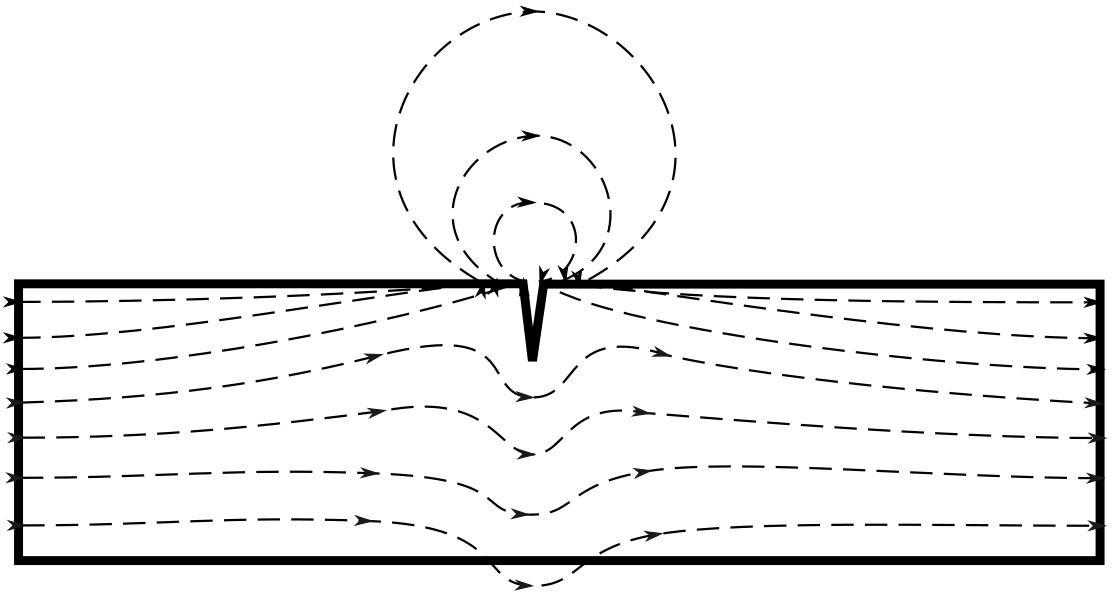
\includegraphics[width=0.9\textwidth]{./Figures/MMM_dispersion}
\vspace{10cm}

{\fontsize{20}{24}\selectfont \textsc{\bfseries Temas de}} 
\vspace{2.0cm} \\ 
{\fontsize{35}{37}\selectfont \textsc{\bfseries Magnetismo }}
\vspace{30px} \\ 
{\fontsize{37}{37}\selectfont \textsc{\bfseries y }}
\vspace{30px}\\ 
{\fontsize{35}{37}\selectfont \textsc{\bfseries Superconductividad }}


%\textsc{\Large Memoria del Trabajo Final}\\[1cm] % Thesis type
\vspace{0.5cm}
%{\huge \bfseries \ttitle \par}




\begin{figure}[H]
    \centering
    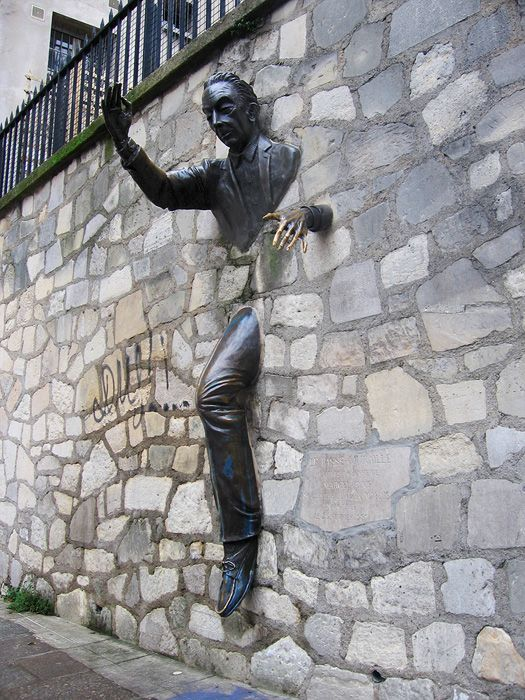
\includegraphics[width=0.60\textwidth]{./Figures/tapaLibro}
 \end{figure}

%\vfill

\vspace{1.5cm}
Ruzzante \\ %\authornameUno
Alonso Castillo \\ %\authornameUno
Suárez Antola \\

\vspace{4.5cm}

\large
%{Director:} \\
%{\supname} % Supervisor name
 
%\vspace{1cm}
%Jurados:\\	
%\jurunoname\\
%\jurdosname\\
%\jurtresname

%\vspace{1.5cm}


\end{center}
%\end{titlepage}



%segunda página
\newpage
\begin{flushleft}
\begin{small}

\vspace{10.0cm} 

\vfill

\textit{Temas de \\ Magnetismo y Superconductividad \\
by \\
José Ruzzante, \\ %\authornameUno
Pablo Alonso Castillo and \\ %\authornameUno
Roberto Suárez Antola}
\vspace{5mm} 

\textit{Copyright} \textcopyright 2020 by the authors
\vspace{5mm} 

\textbf{ISBN:} \\
\textit{Printed in Argentina}
\vspace{5mm} 

Published by the authors\\ 
Alsina 2795, Florida (1602),\\
Buenos Aires.\\
Argentina.\\
(54)9 11 3483 8615
\vspace{5mm} 

Direct Inquires and/or orders to the above address\\
\vspace{5mm} 
All rights reserved. Except for use in a review, no\\
portion of this book may be reproduced in any form\\
without the express written permission of the publisher.\\
\vspace{5mm} 
Neither the authors not the publishers assumes\\
any responsability for the use or misuse of\\
information contained in this book.\\


\end{small}
\end{flushleft} 

%otra página
\frontmatter %Inicia la numeración en números romanos
\begin{titlepage}
\begin{center}


%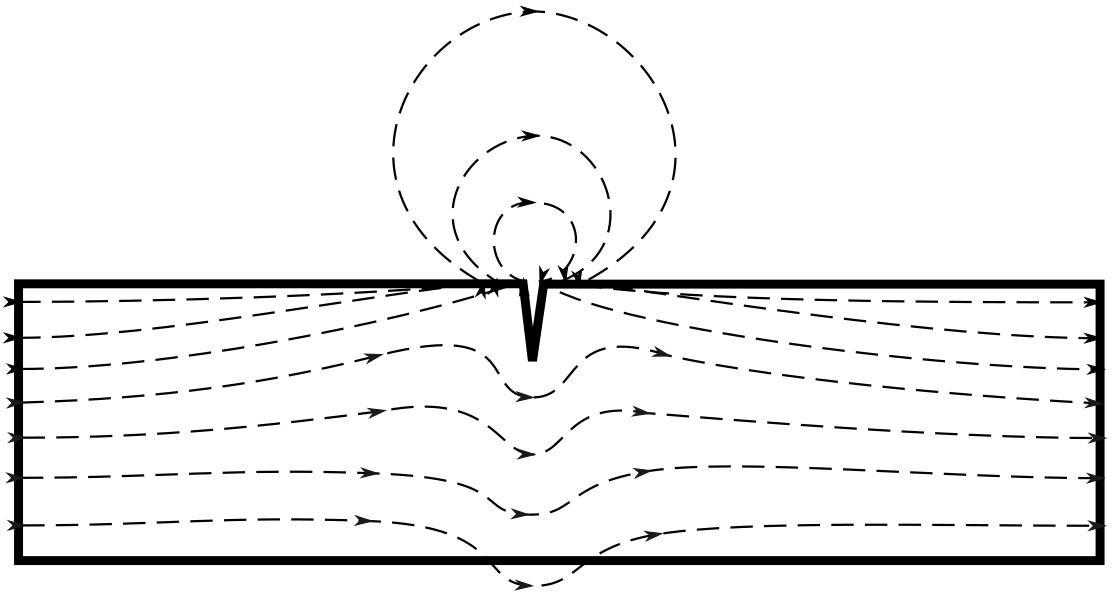
\includegraphics[width=0.9\textwidth]{./Figures/MMM_dispersion}
\vspace{10cm}

{\fontsize{20}{24}\selectfont \textsc{\bfseries Temas de}} 
\vspace{4.0cm} \\ 
{\fontsize{35}{37}\selectfont \textsc{\bfseries Magnetismo }}
\vspace{30px} \\ 
{\fontsize{37}{37}\selectfont \textsc{\bfseries y }}
\vspace{30px}\\ 
{\fontsize{35}{37}\selectfont \textsc{\bfseries Superconductividad }}

\vspace{1.5cm}
Colección de temas al estado del arte en magnetismo y superconductividad con aplicaciones de física pura, química, ciencia de materiales, ensayos industriales y biología. 

\vspace{1.5cm}

%\textsc{\Large Memoria del Trabajo Final}\\[1cm] % Thesis type
%\vspace{1.5cm}
%{\huge \bfseries \ttitle \par}

%\vspace{0.4cm} % Thesis title

%\vfill

\vspace{1.5cm}
\LARGE\textbf{Autores:}\\
Dr. José Ruzzante \\ %\authornameUno
Esp. Pablo Alonso Castillo \\ %\authornameUno
Dr. Roberto Suárez Antola \\

\vspace{4.5cm}

\large
%{Director:} \\
%{\supname} % Supervisor name
 
%\vspace{1cm}
%Jurados:\\	
%\jurunoname\\
%\jurdosname\\
%\jurtresname

%\vspace{1.5cm}

\textit{Buenos Aires 2020}
\end{center}
\end{titlepage}

%----------------------------------------------------------------------------------------
%	RESUMEN - ABSTRACT 
%----------------------------------------------------------------------------------------

%\begin{abstract}
%\addchaptertocentry{\abstractname} % Add the abstract to the table of contents
%
%%
%%The Thesis Abstract is written here (and usually kept to just this page). The page is kept centered vertically so can expand into the blank space above the title too\ldots
%\centering
%
%El Magnetismo y la superconductividad han . . . . .  . 
%
%\end{abstract}


%----------------------------------------------------------------------------------------
%	CONTENIDO DE LA MEMORIA  - AGRADECIMIENTOS
%----------------------------------------------------------------------------------------

%\begin{acknowledgements}
%\addchaptertocentry{\acknowledgementname} % Descomentando esta línea se puede agregar los agradecimientos al índice
%\vspace{1.5cm}
%
%Quiero agradecer  . . . . . 
%  
%
%\end{acknowledgements}

\chapter*{ }

{\larger

\hspace{20mm}Tres clases hay de ignorancia: no saber lo que debiera saberse, saber mal lo que se sabe, y saber lo que no debiera saberse. Si juzgamos el amor por la mayor parte de sus efectos, se parece más al odio que a la amistad. Si no tenemos paz dentro de nosotros, de nada sirve buscarla fuera

\vspace{10mm}
\hspace{7.6cm} François de La Rochefoucauld


%\hspace{20mm}Pocas honras en la vida han sido para mi mayores que la de poder presentar a ustedes esta obra que constituye un verdadero aporte a la formación de los científicos y profesionales en tan diversas áreas como las ciencias exactas, la ingeniería y la biología. En este opus encontrarán, claramente explicados fenómenos, que no por conocidos o publicitados, se encuentren fácilmente en la literatura especializada. Estos temas que constituyen algunos de los pilares de la ciencia y tecnología actuales  han sido resumidos y sistemáticamente expuestos para que el lector avezado, partiendo de los fundamentos mínimos, pueda avanzar hacia la comprensión cabal de los mecanismos subyacentes del magnetismo y la superconductividad. La confío a sus manos con el íntimo convencimiento y satisfacción de que la encontrarán tanto de apasionante interés como de suma utilidad.

%\vspace{10mm}
%\hspace{7.6cm} G.G.J. H\"afelfinger Kontus
}

\chapter*{Prefacio}


{\larger
\hspace{20mm} Este libro se originó como una serie de disertaciones en conferencias y cursos de posgrados que los autores realizaron para . . . .
}

\chapter*{Palabras de los autores}


\hspace{20mm}Toda obra lleva consigo el potencial de influir en los hombres y de perdurar en el tiempo. No pretendo tanto como esto, sino tan solo poder ayudar con mi pequeña contribución a facilitar  algunos temas y dar herramientas para que se tenga una comprensión más acabada de estos fenómenos y sus fundamentos. La capacidad de integrar conocimientos es una rara cualidad que permite grandes avances en áreas poco relacionadas y es cada día mas necesaria por cuanto las fuertes especializaciones a las que ha tendido desde hace décadas la formación universitaria, tienden a producir una visión de túnel en tanto que hemos ingresando a una etapa donde el conocimiento y el progreso se fraguan ampliando la visión y coordinando conocimientos entre distintas áreas. Llegará el día en el futuro cercano en que no será viable separar las ciencias tan claramente como hasta ahora. Espero aquí, haber ayudado a facilitar ese camino.\\


\hspace{9.0cm}Pablo J.C. Alonso Castillo.\\

\vspace{10mm}

%Sic transit gloria mundi.\\

\hspace{9.0cm}José Ruzzante.\\

\vspace{10mm}
	
	
%Ibidem \\

\hspace{9.0cm}Roberto Suárez Antola.\\

\vspace{10mm}




\chapter*{Biografias}

\begin{sloppypar}


$\centerdot$ \textbf{José E. Ruzzante}; es Licenciado en Física, por la Facultad de Ciencias Exactas y Naturales, de la Universidad de Buenos Aires, y recibido de Doctor en Física en la Universidad Nacional de La Plata, Argentina. Se especializó en Emisión Acústica en el CISE, Milán - Italia. Fue Director Científico del “International Centre for Earth Sciences” (ICES) que pertenece a la Comisión Nacional de Energía Atómica (CNEA) y a la Universidad Nacional de Cuyo (UNC), Mendoza – Argentina. Participó, junto a otros dos autores, en la escritura del libro "Ultrasonido y Emisión Acústica para Ingenieros y Estudiantes de Ingeniería", accesible desde: \url{https://www.researchgate.net/publication/341655775_"Ultrasonido-y-Emision Acustica-para-Ingenieros-y-Estudiantes-de-Ingenieria"}. y publicó el libro "Ondas elásticas en sólidos" ISBN 978-987-86-6502-3.
 Actualmente es:  Miembro Fundador del Grupo Latinoamericano de Emisión Acústica (GLEA);  Profesor Consulto de la Universidad Tecnológica Nacional (UTN);  Instructor ASME (American Society of Mechanical Engineers); Profesor Titular en la Universidad Nacional de Tres de Febrero (UNTREF) en la carrera de Ingeniería en Sonido;  Responsable del Grupo de Investigación en Acústica Subacuática (GIAS) de la misma Universidad.
 
$\centerdot$ \textbf{Roberto Suárez Antola}; es Licenciado en Física, Magíster en Biofísica y Doctor en Ciencias Biológicas por la Universidad de la República de Uruguay (UdelaR).  Además posee formación en medicina adquirida en la Facultad de Medicina de UdelaR. Se especializó en ingeniería nuclear, a nivel de posgrado, en la Facultad de Ingeniería de la Universidad de Buenos Aires. Efectuó estudios de profundización en algunos temas de ciencias fisicomatemáticas e ingeniería en Alemania, Austria, España, Francia e Inglaterra.
Fue Profesor Titular y Director de Carrera en UdelaR y en la Universidad Católica del Uruguay. Dirigió los laboratorios de la Comisión Nacional de Energía Atómica y de la Dirección Nacional de Tecnología Nuclear del Ministerio de Industria, Energía y Minería (MIEM). Actualmente es Asesor en el MIEM de Uruguay. Compartió un premio de la Academia Nacional de Medicina, un premio Génesis del MIEM y un premio de la Academia Nacional de Ingeniería de Uruguay. Es autor de un libro sobre energía nuclear y un libro sobre teoría de la relatividad. Publicó artículos de investigación y capítulos de libro en temas de ciencias físico matemáticas, ingeniería y ciencias biomédicas.

$\centerdot$ \textbf{Pablo J.C. Alonso Castillo}; es Licenciado en Física, por la Facultad de Ciencias Exactas y Naturales, Ingeniero Electricista y Especialista en Sistemas Embebidos por la Facultad de Ingeniería, todas de la Universidad de Buenos Aires. Es Profesor Universitario  por la Facultad de Psicología y Pedagogía de la Universidad del Museo Social Argentino. Realizó estudios en los EE.UU., Trabajó como Ingeniero de Campo y Desarrollador de firmware y software para aplicaciones nucleares. Trabaja desde el año 2003 para la Comisión Nacional de Energía Atómica (CNEA), Lideró los desarrollos de diversos proyectos en el área de Plasmas, olfatometría electrónica, espectrometría y monitoreo remoto. Es el responsable del Laboratorio de Espectrometría de Movilidad Iónica (LEMI). Desde el año 2014 es el Secretario Académico del Instituto de Formación Técnica Superior N°14 del GCBA.

\end{sloppypar}


%----------------------------------------------------------------------------------------
%	CONTENIDO DE LA MEMORIA  - DEDICATORIA
%----------------------------------------------------------------------------------------

\dedicatory{\textbf{. . . . Dedicado a . . . . .}}  % escribir acá si se desea una dedicatoria

%----------------------------------------------------------------------------------------
%	CONTENIDO DE LA MEMORIA  - CAPÍTULOS
%----------------------------------------------------------------------------------------

\mainmatter % Begin numeric (1,2,3...) page numbering

\pagestyle{thesis} % Return the page headers back to the "thesis" style

%\renewcommand{\tablename}{Tabla} %TODO eliminar esta línea

% Incluir los capítulos como archivos separados desde la carpeta Chapters
% Descomentar las líneas a medida que se escriben los capítulos


\chapter{Introducción al magnetismo} % Main chapter title

%----------------------------------------------------------------------------------------

% Define some commands to keep the formatting separated from the content 
\newcommand{\keyword}[1]{\textbf{#1}}
\newcommand{\tabhead}[1]{\textbf{#1}}
\newcommand{\code}[1]{\texttt{#1}}
\newcommand{\file}[1]{\texttt{\bfseries#1}}
\newcommand{\option}[1]{\texttt{\itshape#1}}
\newcommand{\grados}{$^{\circ}$}

%----------------------------------------------------------------------------------------



\vspace{0.5cm} 

\begin{flushright}
Yo prefiero ese algo recóndito que alguien del sexo opuesto emitía hacia mi.\\
A ese algo voy a llamarlo aquí “magnetismo”.\\
Una fuerza que te atrae y absorbe, te guste o no te guste, quieras o no\\
Al sur de la frontera, al oeste del Sol\\
Haruki Murakami
\end{flushright}
\vspace{1.0cm} 


 

%$\centerdot$ Creo que lo mas didáctico es desarrolla la primera parte del curso a través de las similitudes que poseen los materiales \textbf{piezomagnéticos} y \textbf{piezoeléctricos}. Si bien los fenómenos no son exactamente iguales poseen algunas similitudes, luego tratamos de explicar el fenómeno magnético Para tal fin exponemos un brevísimo resumen de la mecánica cuántica, ya que el magnetismo atómico es un fenómeno cuántico.
%
%$\centerdot$ En un material piezomagnético, uno puede inducir un momento magnético espontáneo al
%aplicar una tensión mecánica, o bien una deformación física aplicando un campo magnético El \textbf{piezomagnetismo} es un fenómeno que se caracteriza por un acoplamiento lineal entre la polarización magnética y la tensión mecánica.
%
%$\centerdot$  Los materiales piezoeléctricos son aquellos que al ser sometidos a tensiones mecánicas,
%adquiere una polarización eléctrica, luego generan una diferencia de potencial en su superficie.
%
%$\centerdot$ Actualmente se piensa que el piezomagnetismo es un efecto magnetomecánico lineal análogo al efecto electromecánico lineal de la piezoelectricidad De igual manera, la magnetostricción y la electroestricción son efectos análogos de segundo orden. Estos efectos de orden superior se pueden pensarse de primer orden si las variaciones de los parámetros son pequeñas"
%
%Algo realmente importante en estos fenómenos es que son reversibles como se representa en la figura \ref{fig:10}
%
%
%\begin{figure}[H]
%    \centering
%    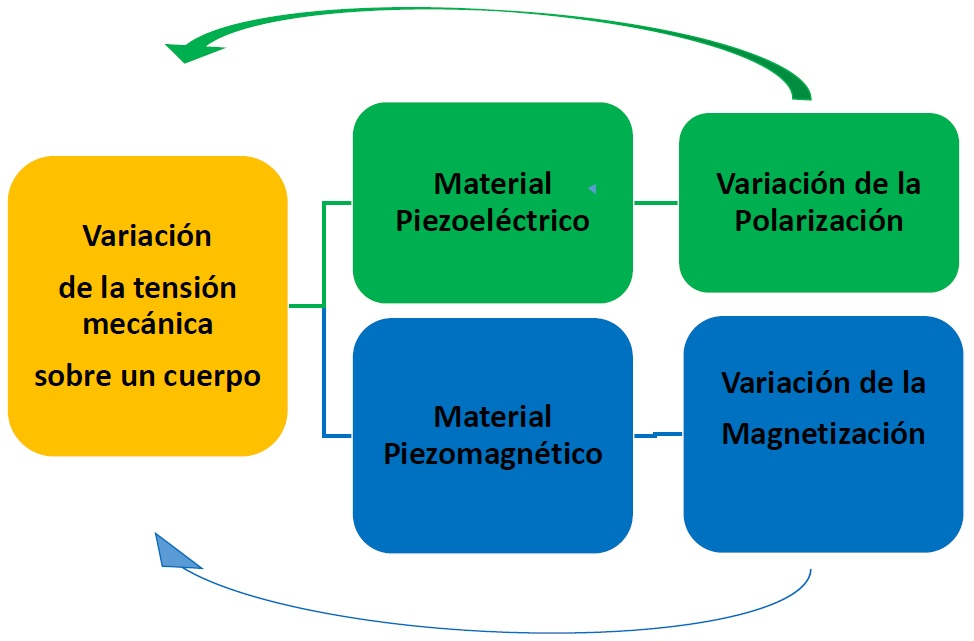
\includegraphics[width=0.80\textwidth]{./Figures/fig10}
%	\caption{Efectos piezoeléctrico y piezomagnético}
%	\label{fig:10}
% \end{figure}
%
%
%\begin{figure}[H]
%    \centering
%    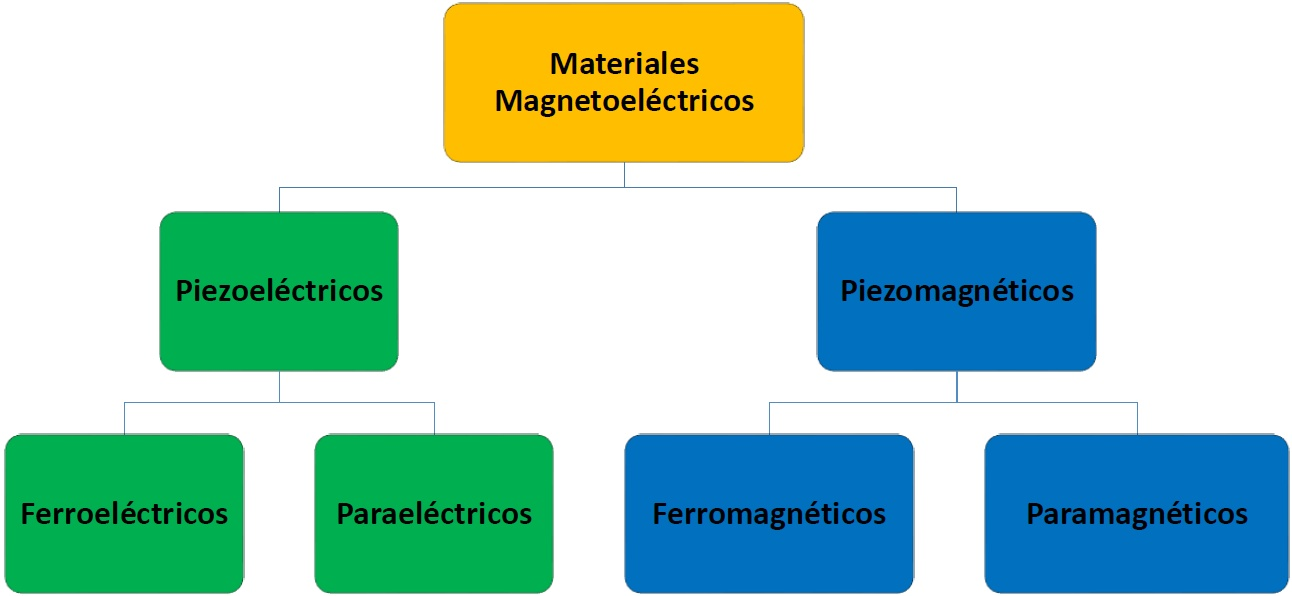
\includegraphics[width=1.0\textwidth]{./Figures/fig11}
%	\caption{Materiales magnetoeléctricos}
%	\label{fig:10}
% \end{figure}
%
%Tratemos de explicar el origen de estos dos fenómenos recordando algunas ideas

\section{Introducción histórica} 

$\centerdot$ Iniciamos este trabajo con un breve e incompleto resumen histórico sobre la idea de átomo.

\begin{itemize}
\item \textbf{Joseph John Thomson} recibió el Premio Nobel de Física en 1906 por el descubrimiento del \textbf{electrón en 1897} Thomson probó que los rayos catódicos tenían naturaleza corpuscular y estaban formados por electrones Curiosamente, su hijo \textbf{George Pagget Thomson} también recibió el Premio Nobel de Física en 1937 por demostrar que el electrón es una onda constituyendo la demostración experimental de la dualidad partícula onda

\item Se atribuye a \textbf{Ernest Rutherford} el descubrimiento del \textbf{protón, en el año 1918} con carga positiva e igual a la del electrón ($1,6\times 10^{-19}$C) Es una partícula subatómica cuya masa e 1836 veces superior a la del electro En la década del 1970 se crean evidencia que es una partícula compuesta.

\item \textbf{James Chadwick} descubre el \textbf{neutrón en el año 1932}, partícula que no tiene carga eléctrica y que junto con el protón constituye el núcleo atómico Su masa es similar a la del protón Fuera del núcleo el neutrón es inestable dura $14,7$ minutos El neutrón es el responsable de la estabilidad de los núcleos.

\item A lo largo de la historia la idea de átomo fue cambiando, desde la propuesta de Dalton en adelante, cada nuevo modelo explicaba algún fenómeno, fallando en otros, ya que nacen de experiencias realizadas. Solo comentaremos los mas recientes.

\item \textbf{J. J. Thomson} luego del descubrimiento del electrón propuso en 1898 que los átomos son esferas de materia con carga positiva embebida de electrones.

\item \textbf{E. Rutherford en 1911} describe al átomo como compuesto por un núcleo, pequeño, de carga positiva con los electrones a cierta distancia exterior
girando, con gran cantidad de espacio vacío La importancia de este modelo es que introducía la existencia de un nucleo atómico.

\item \textbf{Modelo de Niels Bohr en 1913} supone que solo algunas órbitas de los electrones son posibles, con esta hipótesis logra explicar los espectros de emisión y absorción atómicos. Este modelo es clásico pero introduce por primera ves ideas de cuántica Supuso que los electrones solamente se podían mover en órbitas circulares definidas. Cada órbita puede ser identificada mediante un número entero \textbf{n} llamado número cuántico principal.

\item \textbf{Arnold Sommerfeld en 1916} presenta el modelo atómico de Bohr modificado donde introduce orbitas de los electrones elípticas y velocidades relativistas. La excentricidad de la orbita dio lugar al número cuántico azimutal, que establece la forma de los orbitales, se lo representa con la letra \textbf{l} y toma valores que van desde $0$ hasta $n-1$.

\item \textbf{Modelo de Schrödinger 1926} plantea una ecuación de onda para los electrones, que los supone ondas de \textbf{De Broglie}. La solución estacionaria de ecuación de Schrödinger del átomo esta caracterizada por tres números cuánticos \textbf{n}, \textbf{l} y \textbf{m}. Predice adecuadamente las líneas espectrales de distintos tipos de átomos, tanto neutros como ionizados y explica las uniones químicas. Posteriormente \textbf{Max Born 1926} propone la interpretación probabilística de la función de onda de los electrones y \textbf{Dirac en 1928} generaliza la ecuación de Schrödinger agregando la relatividad y dando origen al espín del electrón y su numero cuántico \textbf{s}. Hasta aquí es todo lo que necesitamos saber para entender el átomo.

\end{itemize}


%\section{Tipo de interacción elemental y similitudes}
%\textbf{Dipolo eléctrico}, reacciona ante un $\V{E}$ externo orientándose en la dirección de éste. A grandes distancias del dipolo la intensidad del campo $\V{E}$ disminuye $\left( \dfrac{1}{r^{3}}\right)$ con mayor rapidez que el campo eléctrico eléctrico $\left( \dfrac{1}{r^{2}}\right)$ de una sola partícula cargada.
%
%\begin{figure}[H]
%    \centering
%    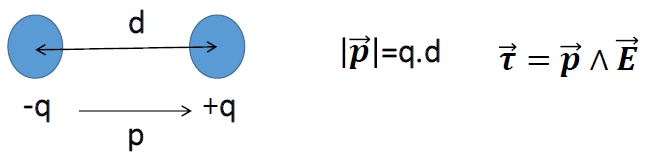
\includegraphics[width=0.80\textwidth]{./Figures/fig12}
%	\caption{Dipolo Eléctrico}
%	\label{fig:13}
% \end{figure}
%
%\textbf{Dipolo magnético} reacciona ante un campo $\V{H}$ externo orientándose en dirección a éste
%También aquí a grandes distancias del dipolo la intensidad del campo $\V{B}$ disminuye $\left( \dfrac{1}{r^{3}}\right)$
%
%\begin{figure}[H]
%    \centering
%    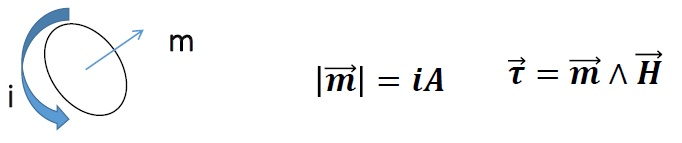
\includegraphics[width=0.80\textwidth]{./Figures/fig13}
%	\caption{Dipolo Magnético}
%	\label{fig:13}
% \end{figure}
%
%\subsection{Dipolos eléctricos y magnéticos}
%
%\begin{itemize}
%
%\item Se ve que existe una coincidencia entre el campo eléctrico creado por dos cargas eléctricas de signo contrario y el campo magnético engendrado por una corriente circular en un anillo, siempre que los miremos desde lejos Luego no fue necesario pensar en la existencia de monopolos magnéticos El dipolo magnético se genera por el movimiento de una carga eléctrica.
%
%\item En el caso de cargas eléctricas la existencia del momento dipolar es un testimonio de la asimetría de la estructura de cargas.
%
%\item Existen átomos o moléculas aisladas que poseen un momento dipolar magnético espontaneo, similarmente hay átomos o moléculas aisladas que poseen un momento dipolar eléctrico estos son llamados paramagnéticos o paraeléctricos respectivamente.
%
%\item El descubrimiento del efecto piezoeléctrico en el cuarzo, dará la posibilidad de generar y recepcionar sonidos a voluntad Este hallazgo fue realizado por los hermanos Pierre y Jacques Curie en 1881 Un tiempo antes 1842 James Prescott Joule descubre el fenómeno piezomagnéticos Este fenómeno tiene características similares al piezoeléctrico Se tardó unos años en encontrar aplicaciones concretas a estos dos fenómenos.
%
%\end{itemize}
%
%\subsection{Formación de los dipolos eléctricos}
%
%\textbf{Dieléctrico}: Es un material mal conductor de electricidad, por lo que puede ser utilizado como aislante eléctrico, además si es sometido a un campo eléctrico externo, puede establecerse en él un campo eléctrico interno No hay cargas libres Todos los materiales dieléctricos son aislantes pero no todos los materiales aislantes son dieléctricos En general hay dos tipos de materiales dieléctricos los que las moléculas, iones o átomos son polares y las que se polarizan por la existencia del campo eléctrico Existen varios mecanismos por intermedio de los cuales se polarizan los materiales, no entraremos en mas detalles.
%
%\begin{figure}[H]
%  \centering
%  \begin{minipage}[b]{0.47\textwidth}
%    \centering
%     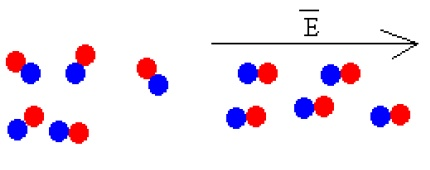
\includegraphics[width=1.0\textwidth]{./Figures/fig14}
%	 \caption{\protect\raggedright Moléculas polares.}
%	\label{fig:14}
%  \end{minipage}
%  \hfill
%  \begin{minipage}[b]{0.47\textwidth}
%    \centering
%     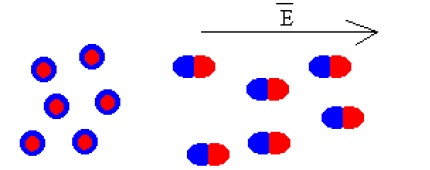
\includegraphics[width=1.0\textwidth]{./Figures/fig15}
%	 \caption{\protect\raggedright Moléculas no polares.}
%	\label{fig:15}
%  \end{minipage}
%\end{figure}
%
%
%La molécula de agua, tiene una distribución asimétrica de sus electrones, lo que la convierte en una molécula polar, alrededor del oxígeno se concentra la nube de carga negativa, mientras que los núcleos de hidrógeno quedan desprovistos parcialmente de sus electrones, luego, manifiestan, una densidad de carga positiva Por tanto la molécula de agua es dipolar Las moléculas polares pueden formar compuestos químicos, cuando interactúan entre si, las fuerza que manifiestan los dipolos se llama de fuerza de Van der Waals.

\section{Formulación matemática}

Maxwell logra, en el siglo 19 expresar matemáticamente los hallazgos de Faraday y engloba todos los fenómenos clásicos del electromagnetismo en sus ecuaciones, concibe las ondas electromagnéticas y determina su velocidad


\begin{equation*}
\label{eq:100}
\begin{aligned}
	\nabla \times \overrightarrow{H} = \overrightarrow{J_{c}} + \dPv{D}{t} 
	\quad \quad
	&\nabla \times \overrightarrow{E} = - \dPv{B}{t} 	\\
	\nabla \cdot \overrightarrow{B}=0
	\quad \quad
	&\nabla \cdot \overrightarrow{D} = \rho_{l}
\end{aligned}
\end{equation*}

\begin{equation*}
	\V{f}= q(\V{E}+\V{v}\times\V{B})
\end{equation*}

Se ve que una corriente eléctrica genera un campo magnético, dicho de otro modo el movimiento de cargas eléctricas genera un campo magnético, luego existe una relación entre movimiento de cargas y campo magnético, ¿que podría explicar el magnetismo atómico?

$\V{E}$ Campo eléctrico en el espacio, $\V{D}$ Denota efectos eléctricos en la materia \\
$\V{H}$ Campo magnético en el espacio, $\V{B}$ Campo magnético en la materia \\
$\V{f}$ fuerza de Lorentz.

Parecería que con las ecuaciones de Maxwell se tendría la descripción total del magnetismo atómico. !No es así¡ El magnetismo en los sólidos es un fenómeno cuántico. Muchos de los fenómenos magnéticos solo se pueden explicar cuánticamente Un modelo atómico Borh simple considera al electrón girando alrededor del núcleo atómico muy pequeño El núcleo contiene toda la carga positiva del átomo Las ecuaciones de Maxwell sugieren que un electro acelerado debe radiar energía con una frecuencia fundamental y otras armónicas múltiplo de la fundamental Si el movimiento del electrón es circular (y por tanto acelerado) y uniforme, emitiría una sola frecuencia, luego el electrón perdería energía y colapsaría Tampoco podemos explicar la estabilidad del núcleo atómico con tantas cargas positivas juntas

Sabemos que los fenómenos de óptica se deben tratar de dos maneras distintas según el caso si la dimensión del objeto es mucho mayor que la longitud de onda de la luz, podemos utilizar la óptica geométrica y definir trayectorias bien precisas, la luz se la trata como una partícula, por el contrario si la longitud de onda de la luz es comparable con la dimensión del objeto, aparecen los fenómenos de difracción y no se puede utilizar la óptica geométrica No podemos definir una trayectoria ni afirmar que son partículas Si aceptamos este tipo de comportamiento para el micro mundo, entonces la longitud $\lambda$ de un determinado ente esta dada por la expresión:

\begin{equation}
	\lambda=\dfrac{h}{mv}
\end{equation}

Donde $h\approx 6,62607015 \times 10^{-34}\left[ Js\right]$ es la constante de Planck, $m$ la masa y $v$ la velocidad.

Veamos si tiene sentido tratar a una bolita de $1gr$ que se mueve a una velocidad de $1\frac{cm}{s}$ como una onda, calculando $\lambda=6,6\times10^{-27}cm$. Totalmente despreciable frente al tamaño del cuerpo. Tendremos fenómenos de difracción en zonas de dimensiones comparables con las longitudes de onda. Si realizamos el mismo calculo para los átomos vemos que la longitud de onda es comparable a la dimensión atómica, por tanto, debemos abandonar la idea de trayectoria del electrón bien definida girando a una distancia fija del núcleo. Veamos otro ejemplo:

Supongamos electrones en un tubo de RX que son acelerados con una diferencia de potencial de $10kV$ luego:

\begin{equation}
	eV = h \nu = h\dfrac{c}{\lambda}
\end{equation}


De donde $\lambda$ será:

\begin{equation}
	\lambda =\dfrac{ch}{eV} = 1.239\times 10^{-10} m
\end{equation}

Esto lleva a pensar que la materia tiene propiedades de partícula y de onda, lo que comúnmente se llama dualidad partícula onda pero ¡no significa que sean al mismo tiempo las dos cosas!. Estas ondas se llaman ondas de De Broglie o de materia. Lo único que podemos afirmar es que todo ente en
movimiento, bajo cierto experimento se comporta como onda y bajo otro experiencia como particular Tengamos en cuenta que estos fenómenos nos son percibidos directamente por nuestros sentidos En la figura \ref{fig:16} tenemos las tres proyecciones de un objeto que esta dentro de la esfera, ¿quien puede decir que es?. 

\begin{figure}[H]
    \centering
    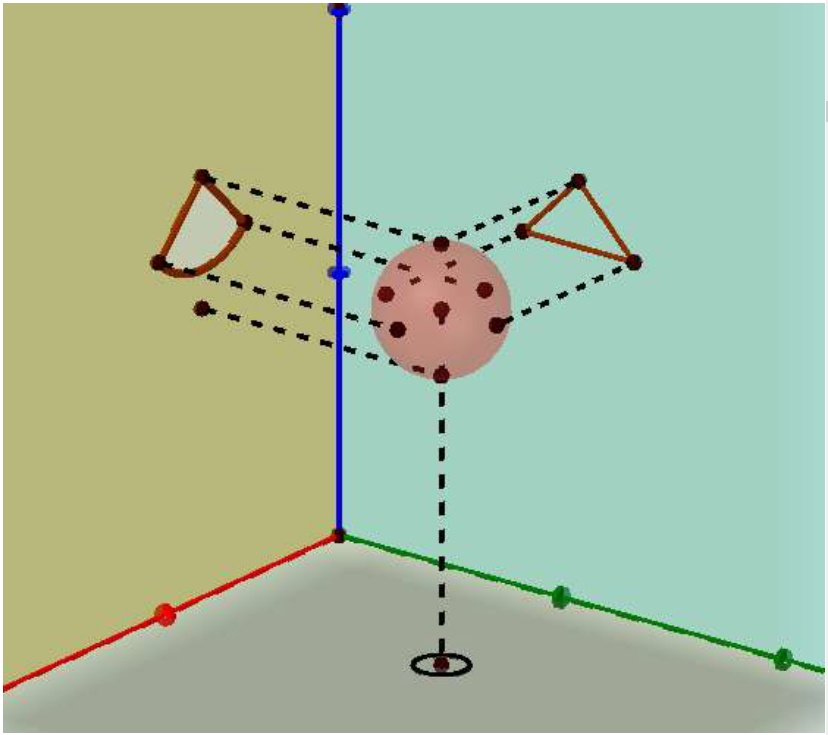
\includegraphics[width=0.80\textwidth]{./Figures/fig16}
	\caption{Proyecciones en tres planos}
	\label{fig:16}
 \end{figure}


Las características ondulatoria y corpuscular son complementarias y excluyentes, nuestro conocimiento de las particularidades es parcial si solo utilizamos uno de ellos. 

No debemos explicar el micromundo en función de conceptos del macromundo como son las ondas puras o partículas puras, solo será posible comprender el átomo si pensamos en el comportamiento corpuscular de las ondas y en el comportamiento ondulatorio de las partículas.

¿Como hallamos esta onda de De Broglie que caracteriza el fenómeno?, por intermedio de la ecuación
diferencial de Schrödinger La solución de esta ecuación nos da lo que llamamos función de onda $\Psi$  que en un punto del espacio y en un instante de tiempo nos da la probabilidad de encontrar la entidad en ese lugar e instante.

La solución de la ecuación de Schrödinger es normalmente un problema complicado Sin embargo, su solución dio excelentes resultados y predijo fenómenos observados experimentalmente imposibles de explicar con la física clásica. Mencionemos un par de ejemplos:

1.- La ecuación Schrödinger independiente del tiempo, para un caso unidimensional tiene el
siguiente aspecto:

\begin{equation}
	\dfrac{d^{2}\Psi}{dx^{2}} + \dfrac{2m}{\hbar^{2}}\big( E-V(x) \big)\Psi = 0
\end{equation}

Donde $m$ es la masa, $V(x)$ la energía potencial, $E$ la energía total del sistema y $\hbar=\dfrac{h}{2\pi}$. La solución de la ecuación no solo depende de la función $V(x)$ sino también del valor numérico de $E$. Para cualquier valor de $E$ no es posible encontrar una solución $\Psi$ continua y con condiciones de probabilidad, luego se comprueba que solo hay solución para valores discretos de la energía $E_{1}$, $E_{2}$, $E_{3}, \cdots E_{n}$. La energía toma valores discretos, esta
cuantificada y se los llama valores propios, siendo $\Psi_{1}$, $\Psi_{2}$, $\Psi_{3}, \cdots \Psi_{n}$ las funciones propias o características

2.- Suponiendo ahora un pozo cuadrado de potencial como el que se muestra en la figura \ref{fig:17}
Resolviendo la ecuación de Schrödinger para este potencial, se observa los niveles de energía en color
azul y en rojo una función propia particular, indicando que existe la posibilidad de encontrar al ente
fuera del pozo, fenómeno observado en los núcleos radiactivos que emiten partículas alfa Efecto que
no se explica en la mecánica clásica, efectivamente, ya que

\begin{equation}
	E=\dfrac{m}{2}v^{2} + V \therefore v= \sqrt{\dfrac{2}{m}\left( E-V(x) \right)} 
\end{equation}

\begin{figure}[H]
    \centering
    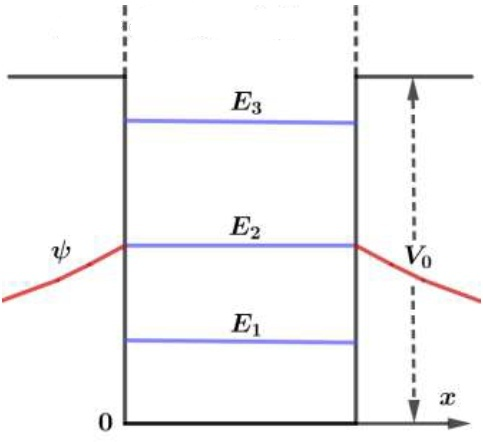
\includegraphics[width=0.60\textwidth]{./Figures/fig17}
	\caption{Pozo de potencial}
	\label{fig:17}
 \end{figure}

Dentro
del pozo $E>V$ ya que el potencial es cero, pero fuera tiene el valor $V_{0}>E$ por tanto la velocidad $v$ seria imaginaria, lo que no tiene sentido, luego clásicamente no podría salir del pozo.

Si el potencial es infinito (paredes totalmente rígidas), caso que no se da en la practica, no se debe
esperar penetración fuera del pozo

3.- Efecto túnel, este fenómeno es también netamente cuántico no apreciado en la mecánica clásica, por ejemplo, si tenemos electrones confinados por una barrera de potencial, únicamente aquellos electrones que excedan en energía la barrera de potencial podrán escapar, clásicamente Si por medio de la ecuación de Schrödinger calculamos la probabilidad de encontrar un electrón del otro lado de la barrera veremos que esta probabilidad no es cero.

\begin{equation}
	\dfrac{\vert\Psi_{b}\vert^{2}}{\vert\Psi_{a}\vert^{2}} \approx e^{-2\sqrt{\dfrac{2m(V_{0}-E}){\hbar^{2}}}W} 
\end{equation}

\begin{figure}[H]
    \centering
    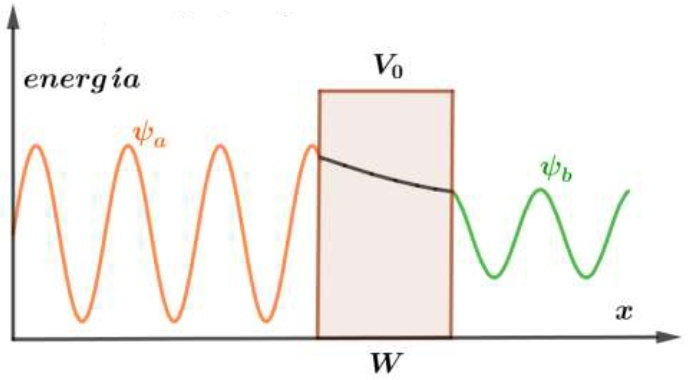
\includegraphics[width=0.80\textwidth]{./Figures/fig18}
	\caption{Efecto túnel}
	\label{fig:18}
 \end{figure}

\section{Números cuánticos}

Estamos en condiciones de entrar en la teoría cuántica atómica y entender el origen del magnetismo atómico, como también, comprender la tabla periódica de los elementos y las uniones químicas. Para ello pensemos en un campo central de fuerza, eléctricas, el mas simple, un protón como núcleo y un electrón, átomo de hidrogeno, como en el modelo de Bohr. En un campo central electrostático sabemos que el potencial depende solo de la distancia al centro. Resolviendo la ecuación de Schrödinger en el espacio (es fácil decirlo) se encuentran tres números cuánticos, alguno de ellos coincide con lo postulado por Bohr Por tanto, los podemos enumerar.

\begin{itemize}
	\item[1]$n=1, 2, 3, \cdots$ número cuántico principal
	\item[2]$l=0, 1, 2, \cdots (n-1)$ número cuántico orbital
	\item[3]$m_{l}=0, \pm 1,\pm 2, \cdots \pm l$ número cuántico magnético
\end{itemize}

\textbf{Número cuántico principal $n$}
La energía del átomo de hidrogeno se cuantifica con el número $n$ por una expresión similar a la supuesta por Bohr

\begin{equation}
	E_{n}= \dfrac{me^{4}}{8\epsilon_{0}^{2}h^{2}} \left(\dfrac{1}{n^{2}} \right) 
\end{equation}

Como vemos no es posible tomar cualquier energía.

\textbf{Número cuántico orbital $l$}

Sabemos que en la mecánica Newtoniana el momento angular en un campo central se mantiene constante con el tiempo a medida que el sistema va cambiando y está dado por la expresión:

\begin{equation}
	\V{L}= \V{r} \times \V{p} = \V{r} \times m \V{v} 
\end{equation}

Luego puede variar la velocidad y $\V{r}$ de cualquier forma, si se manteniendo constante $\V{L}$ En mecánica cuántica al igual que la energía también se conserva el momento angular Las leyes clásicas de conservación tienen su equivalente cuántico, hay leyes de conservación cuántica que no tienen
análogo clásico El número cuántico $l$ informa de la cuantificación del módulo del momento angular del electrón en su órbita dado por la expresión:

\begin{equation}
	\vert\V{L}\vert = \sqrt{l(l+1)} \hbar
\end{equation}

Vemos que la unidad natural del momento angular es $\hbar= 1,054 \times 10^{−34}[Js]$.

Generalmente y como un legado de la espectroscopia se designa a los valores de $l$ con letras en minúscula de tal manera que $l=0\rightarrow s$, $l=1\rightarrow p$, $l=2\rightarrow d$. Un estado $s$ tiene momento angular cero, un estado $p$ tiene momento angular $2\hbar$ El vector $\V{L}$ es perpendicular al plano que contiene el movimiento.

\textbf{Número cuántico magnético $m_{l}$}

La componente del momento angular en una dirección determinada, por ejemplo $z$ es $L_{z}$ y esta determinada por el numero cuántico magnético $m_{l}$ por medio de la expresión siguiente: 

\begin{equation}
	L_{z}= m_{l} \hbar
\end{equation}

Luego la componente $L_{z}$ del momento angular no se orienta en cualquier dirección del espacio, esta cuantificada, como $m_{l}$ puede ser positivo o negativo hay ($2l+1$) orientaciones del vector $\V{L}$. En mecánica clásica, como fue dicho, el $\V{L}$ en un campo central es constante en modulo y dirección, en cuántica solo conocemos el modulo y una componente $L_{z}$ lo que impide conocer la dirección exacta de $L$ Como solo podemos conocer $\vert\V{L}\vert$ y $L_{z}$ imaginamos al vector $\V{L}$ realizando una precesión alrededor del eje $z$.
 
Supongamos el caso de $l=2$ entonces será:

\begin{equation*}
	\vert\V{L}\vert = \sqrt{l(l+1)} \hbar = \sqrt{6}\hbar = 2,45\hbar
\end{equation*}



%Comenzaremos estudiando el magnetismo en átomos, iones, moléculas, para luego pasar a los sólidos. El magnetismo es un fenómeno netamente cuántico en el sentido que debe ser explicado desde esta teoría, sin embargo, unos pocos fenómenos pueden explicase con la física clásica y así lo haremos.
%
%Nuestro mundo macroscópico está constituido por cuerpos y ondas, los cuerpos a su vez por partículas. Tenemos una clara noción de lo que llamamos partícula y onda, las vemos la sentimos y las tocamos. En el caso del mundo microscópico nada de esto es factible, solo es posible interpretar algo a través del comportamiento. ¿Qué otra imagen del micro mundo podemos construir si solo conocemos partículas y ondas?, pero ¿realmente que es? o sea la esencia no lo conocemos. Se trata de interaccionar con el sistema estudiado y de acuerdo a su respuesta interpretar como está constituido.
%
%La Mecánica Cuántica logra describir correctamente los fenómenos atómicos, es decir, en correspondencia con el experimento. De esta manera nace y se desarrolla la mecánica cuántica.
%
%Sin tener nada que ver con nuestro tema y aludiendo a cuestiones filosóficas, mucho tiempo antes de que se gestara la mecánica cuántica (1612), Galileo Galilei escribe una carta a un amigo diciendo: “\textit{Non tentare le essenze, ma contentarsi delle affezioni quantitative}”\footnote{No investigar la esencia, sino contentarse con los efectos cuantitativos}, lo cual es aplicable, también, a nuestro caso.
%%----------------------------------------------------------------------------------------
%
%%\section{Contexto y motivación.}
%
%\section{Magnetismo de iones y átomos libres}
%
%\begin{itemize}
%	\item El magnetismo es un fenómeno cuántico, muchos de los fenómenos magnéticos solo se pueden explicar cuánticamente.
%	\item Un modelo atómico simple considera al electrón girando alrededor del núcleo atómico, esto genera un momento angular orbital $\overrightarrow{\textit{L}}$, podemos tener una imagen bastante real si consideramos al electrón
%girando sobre si mismo, esto genera el momento angular de espín $\overrightarrow{\textit{S}}$. Son dos momentos angulares distintos.
%	\item Es conocido que una corriente eléctrica genera un campo magnético, dicho de otro modo el movimiento de cargas eléctricas genera un campo magnético, luego existe una relación entre movimiento de cargas y campo magnético.
%
%	\item Esta relación es generada por que el electrón posee carga eléctrica y un momento magnético. Este fenómeno posibilitara aplicaciones que se verán más adelante (materiales ferroicos).
%	\item Es en esta relación donde debemos buscar el origen atómico del magnetismo.
%\end{itemize}
%
%
%\subsection{Momento angular orbital}
%
%El momento angular orbital $\overrightarrow{\textit{L}}$ es un vector con módulo:
%
%\begin{equation}
% |\overrightarrow{L}| = \sqrt{l \big(l+1\big) } \, \frac{h}{2 \pi } = \sqrt{l \big(l+1\big) } \, \hbar 
%\end{equation}

Las distintas posiciones del vector $\V{L}$ en el espacio están definidas por el número cuántico orbital $l$ que toma valores entre:

\begin{equation}
 l = 0, 1, 2, 3 \ldots\big(n-1\big) \quad y \quad \hbar = \frac{h}{2 \pi }
\end{equation}


La proyección del vector $\overrightarrow{\textit{L}}$ respecto del eje $z$ en el espacio están definidas por el número cuántico magnético $m_{l}$ que varía entre:

\begin{equation}
 -l,\ldots,0 ,\ldots, +l \quad \text{o sea:} \quad -2,-1,0,+1,+2
\end{equation}

El valor del vector $\V{L_{z}}$ (la dirección del eje $z$ es determinada por un campo magnético externo), está dada por la expresión:

\begin{equation}
	L_{z}=m_{l}\hbar
\end{equation}

Donde $m_{l}$ varia $m_{l}=0, \pm 1, \pm 2, \pm 3, \cdots, \pm l$

\begin{figure}[H]
    \centering
    \includegraphics[width=0.60\textwidth]{./Figures/Gráfico3}
	\caption{Momento angular sus proyecciones}
	\label{fig:Grafico3}
\end{figure}

Para conocer exactamente la dirección de $\V{L}$ es necesario conocer no solo $L_{z}$, si no también $L_{x}$ y $L_{y}$, pero, la Mecánica Cuántica demuestra que es imposible conocer mas de una componente de $\V{L}$. Observemos que $\V{L}$ nunca puede tener la dirección de $z$ o sea coincidir con el campo
magnético, en ese caso conoceríamos las tres componentes.

En la figura \ref{fig:129} tenemos una representación más realista que la anterior.

\begin{figure}[H]
    \centering
    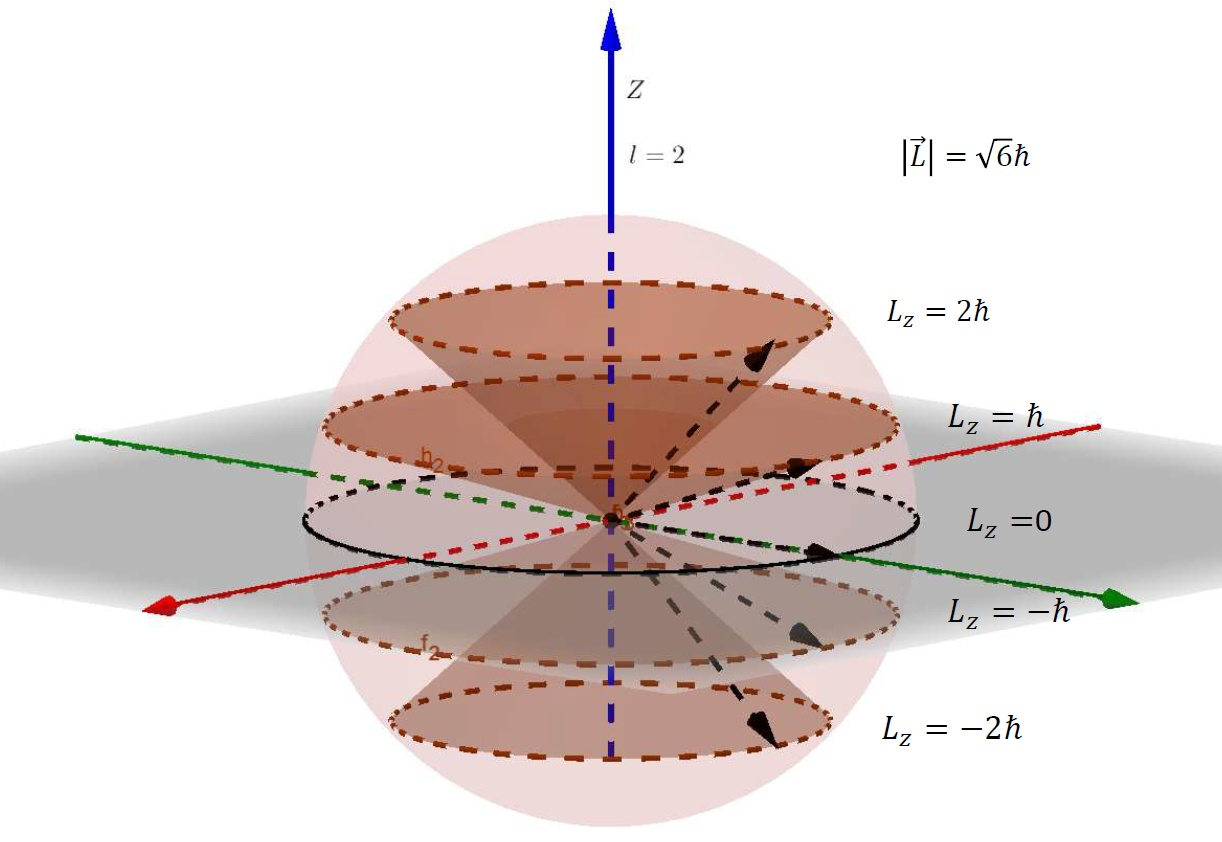
\includegraphics[width=1.0\textwidth]{./Figures/fig129}
	\caption{Momento angular sus proyecciones en 3D}
	\label{fig:129}
\end{figure}

\textbf{Número cuántico $s$}

Un tema aparte es el llamado espín. Este es esencialmente cuántico y hace referencia a una característica intrínseca (i.e. inherente; se refiere a una propiedad física de las partículas subatómicas, por la cual toda partícula elemental o compuesta que se comporte como elemental tiene un momento angular intrínseco de valor fijo Se trata de una propiedad individual de la partícula como lo es la masa o la carga eléctrica). El espín no sale naturalmente de la solución de la ecuación de Schrödinger, que vimos anteriormente. Por supuesto que fue necesario introducirlo para lograr una descripción completa de determinadas observaciones espectrales y entender a los átomos con mas de un electrón En el año 1928 P. Dirac propuso una ecuación cuántica relativista, desde la cual se deriva naturalmente la existencia del espín. P. Dirac pensaba que toda ley física debería tener belleza matemática o sea simetría, generalidad, Esta particularidad tenía su ecuación, lo cual implicaba una novedosa consecuencia, la existencia de una partícula simétrica al electrón con igual masa y similar carga eléctrica, pero positiva. Esta partícula cuando se encuentra con su simétrica un electrón se aniquila liberando la energía de ambas partículas en forma de rayos $\gamma$. Dirac, sin conocerla ni haberla visto profetizo la existencia de la antimateria, tan solo fue sugerida por su ecuación matemática y la idea de simetría. Carl Anderson descubre la primera antipartícula en 1932.

Al espín los podemos interpretar como el momento angular intrínseco de la partícula en reposo. Llamamos $\V{S}$ al espín del electrón y su modulo será

\begin{equation}
 |\V{S}| = \sqrt{s \big(s+1\big) } \, \frac{h}{2 \pi } = \sqrt{s \big(s+1\big) } \,s\hbar 
\end{equation}

Expresión similar a la del momento orbital $|\V{L}|$, donde $s$ es el número cuántico de espín, cuyo valor es $\frac{1}{2}$ para el electrón. También se lo mide en unidades de $\hbar$.
 
\begin{equation}
 |\V{S}| = \sqrt{s \big(s+1\big) } \, \frac{h}{2 \pi } = \frac{\sqrt{3}}{2}\, \hbar
\end{equation}

Esto no tiene nada de clásico, el modulo adquiere un solo valor y si lo interpretamos como el momento angular obserbamos que no puede modificar su velocidad de giro, clásicamente inexistente.

También aquí la componente $S_{z}$ del momento angular de espín de un electrón a lo largo del eje $z$ determinada por un campo magnético exterior está cuantificada y puede tomar dos valores según el número cuántico magnético de espín $m_{s}$, para $m_{s}=+\dfrac{1}{2}$ y $m_{s}=-\dfrac{1}{2}$:

\begin{equation}
 S_{z} = m_{s} \hbar = \pm \frac{1}{2} \hbar
\end{equation}

En la figura \ref{fig:Gráfico2corregido} se observa las posiciones posibles del vector momento angular del electrón:

\begin{figure}[H]
    \centering
    \includegraphics[width=0.60\textwidth]{./Figures/Gráfico2corregido}
	\caption{Momento angular de espín y sus proyecciones}
	\label{fig:Gráfico2corregido}
\end{figure}

Estas propiedades no pueden ser explicadas por modelos clásicos. Si se explican combinando ideas de la Mecánica Cuántica y la Relatividad. (Dirac , 1928)\footnote{En 1928 Dirac reformula el tratamiento de Schrödinger para el átomo monoelectrónico de tal forma que las ecuaciones fueran consistentes con los requerimientos de la teoría de la relatividad. De las soluciones a las ecuaciones de Dirac surgían, de forma natural, los tres números cuánticos ya conocidos $(n, l, ml)$ más un cuarto número cuántico $(s)$ relacionado con esta propiedad intrínseca del electrón que denominamos espín.}.











En mecánica clásica el $\V{L}$ en un campo central es constante en modulo y dirección, en cuántica solo conocemos el modulo y una componente $L_{z}$, lo que impide conocer la dirección exacta.
Como solo podemos conocer $|\V{L}|$ y $L_{z}$ imaginamos al vector $\V{L}$ realizando una precesión alrededor del eje $z$




\subsection{Momento magnético orbital del electrón}

Los momentos angulares de partículas cargadas tiene asociado un momento magnético, cuyo sentido es opuesto al del vector $\V{L}$. Según el electromagnetismo el momento magnético asociado al momento angular orbital del electrón es (como se verá)

\begin{equation}
	\V{\mu_{l}} = \frac{-e\hbar}{2m} \, \V{L}= -\mu_{B} \V{L}
\end{equation}

donde $e$ es la carga del electrón y $m$ la masa del electrón en reposo y $\mu_{B}=\dfrac{e\hbar}{2m}$ es llamado Magnetón de Bohr (unidades atómicas del momento magnético). El signo $–$ significa que los vectores tienen sentido contrarios. Pasando a modulo:

\begin{equation}
 |\overrightarrow{\mu_{l}}| = \sqrt{l \big(l+1\big) } \,  \frac{-e\hbar}{2m} = \sqrt{l \big(l+1\big) } \, \mu_{B} 
\end{equation}

La proyección del momento magnético orbital en la dirección de $z$ es:

\begin{equation}
	\mu_{l_{z}} = -m_{l}\mu_{B}
\end{equation}

\begin{figure}[H]
    \centering
    \includegraphics[width=0.60\textwidth]{./Figures/Gráfico1}
	\caption{Momento angular y momento magnético orbital}
	\label{fig:Grafico1}
 \end{figure}

El electrón en su orbita puede pensarse como un imán solo si $l\neq 0$, si $l=0$ no existe trayectoria, tiene $\vert\V{L}\vert$ en su estado fundamental.


\subsection{Momento magnético del spín del electrón}

Para el electrón, que tiene carga y momento angular se podría espera algo similar a lo obtenido con el momento magnético orbital Sin embargo la expresión clásica no se cumple cuánticamente y es necesario multiplicar por un factor llamado $g_{e}$  de Landé, cuyo valor según Dirac es $G_{e}=2$. Luego el momento magnético del espín es \textbf{exactamente el doble que la del electrón en su movimiento orbital}.

\begin{equation}
	\V{\mu_{S}} = g_{e} \dfrac{-e\hbar}{2m}\V{S} = -g_{e}\mu_{B}\V{S}
\end{equation}

Pasando a modulo:

\begin{equation}
	\vert\V{\mu_{S}}\vert = \sqrt{s(s+1)} \dfrac{e\hbar}{m} = \dfrac{e\sqrt{3}}{2m} \hbar = \sqrt{3} \mu_{B}
\end{equation}

La proyección de este momentos magnético de espín, según una dada dirección del espacio z determinada por un campo magnético externo es:

\begin{equation}
	{\mu_{S}}_{z} = -m_{S} \mu_{B}
\end{equation}

En este caso $m_{S}=\pm \dfrac{1}{2}$, o sea que toma solo dos valores. Estamos en presencia de un imán elemental, \textbf{en la mayoría de los casos el electrón puede ser considerado como un imán elemental}.

Si bien introducimos algunas ideas de la física cuántica no se realizo una demostración exacta de los resultados presentados En la mayoría de los casos los esquemas son semi cuánticos y las expresiones matemáticas también Es el momento de presentar el momentos magnéticos del electrón en su movimiento orbital y el del electrón asociado al espín Si aceptamos una hipótesis del electromagnetismo clásico que indica Los momentos angulares de partículas cargadas tiene asociado un momento magnético, cuyo sentido es opuesto al del vector momento angular. Ver figura \ref{fig:13}

\begin{figure}[H]
    \centering
    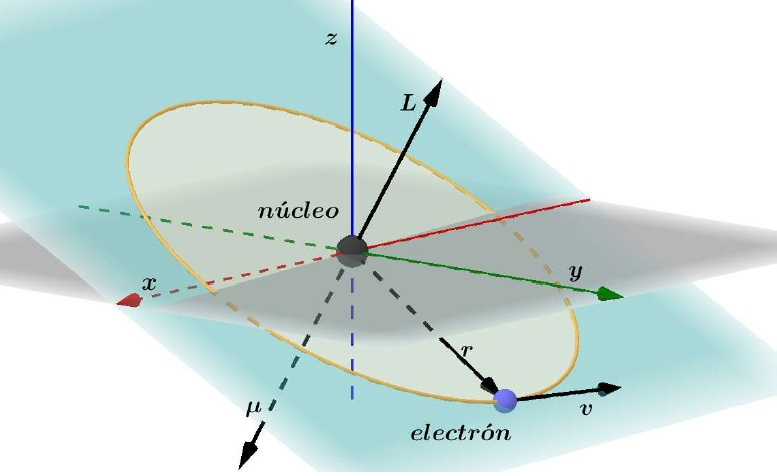
\includegraphics[width=0.9\textwidth]{./Figures/fig113}
	\caption{Momento angular del electrón}
	\label{fig:113}
 \end{figure}

En el caso del momento magnético orbital es aceptable la imagen clásica del electrón con carga eléctrica que al girar genera el momento magnético Para el caso del momento magnético del espín en el electrón, también podríamos aceptar que su momento angular genera un momento magnético, pero la hipótesis clásica se pierde al ver que el momento magnético de espín existe en partículas sin carga, como el fotón y el neutrón. Sin embargo estas suposiciones son de suma utilidad para explicar efectos macroscópicos del magnetismo, y otros fenómenos como la resonancia magnética nuclear En la figura \ref{fig:114} se muestra un esquema del espín y del momento angular orbital en un átomo La magnitud de los vectores no son reales

\begin{figure}[H]
    \centering
    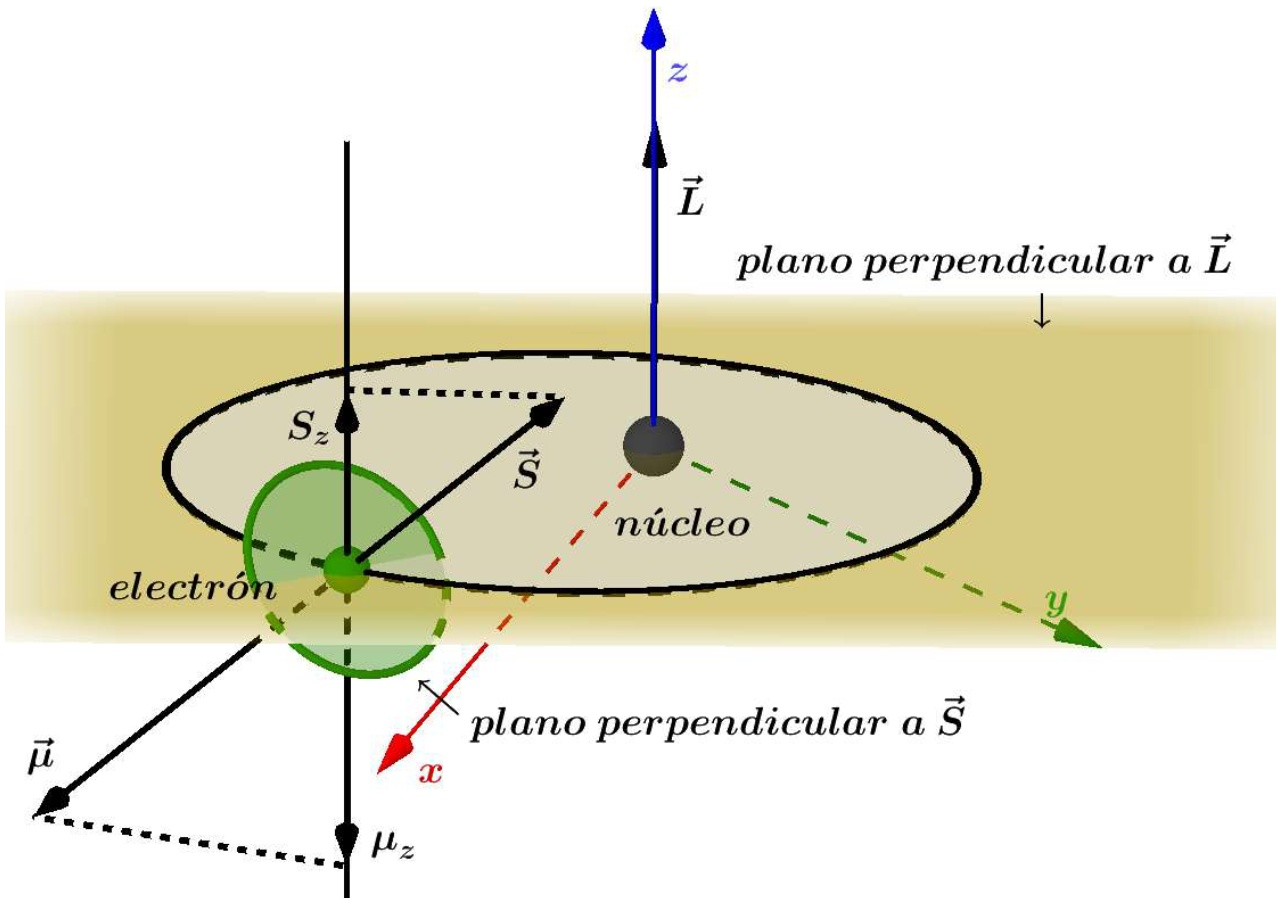
\includegraphics[width=0.9\textwidth]{./Figures/fig114}
	\caption{Espín y momento angular}
	\label{fig:114}
 \end{figure}


Para el electrón, que es una partícula cargada, se podría espera algo similar a lo obtenido en el momento magnético orbital, pero no, el momento magnético de espín, al igual que la masa o la carga del electrón, es una propiedad intrínseca fundamental\footnote{Existen partículas neutras sin carga eléctrica como el neutrón que sin embargo tienen momento magnético (de hecho el neutrón no se considera realmente elemental sino formado por tres quarks cargados fraccionariamente)}. Si fuera el caso clásico su valor seria 1 pero en realidad es un poco mayor de 2 (da exactamente 2 aplicando la ecuación de Dirac y con la corrección de los efectos cuánticos del campo electromagnético un poco más de 2).


\begin{figure}[H]
    \centering
    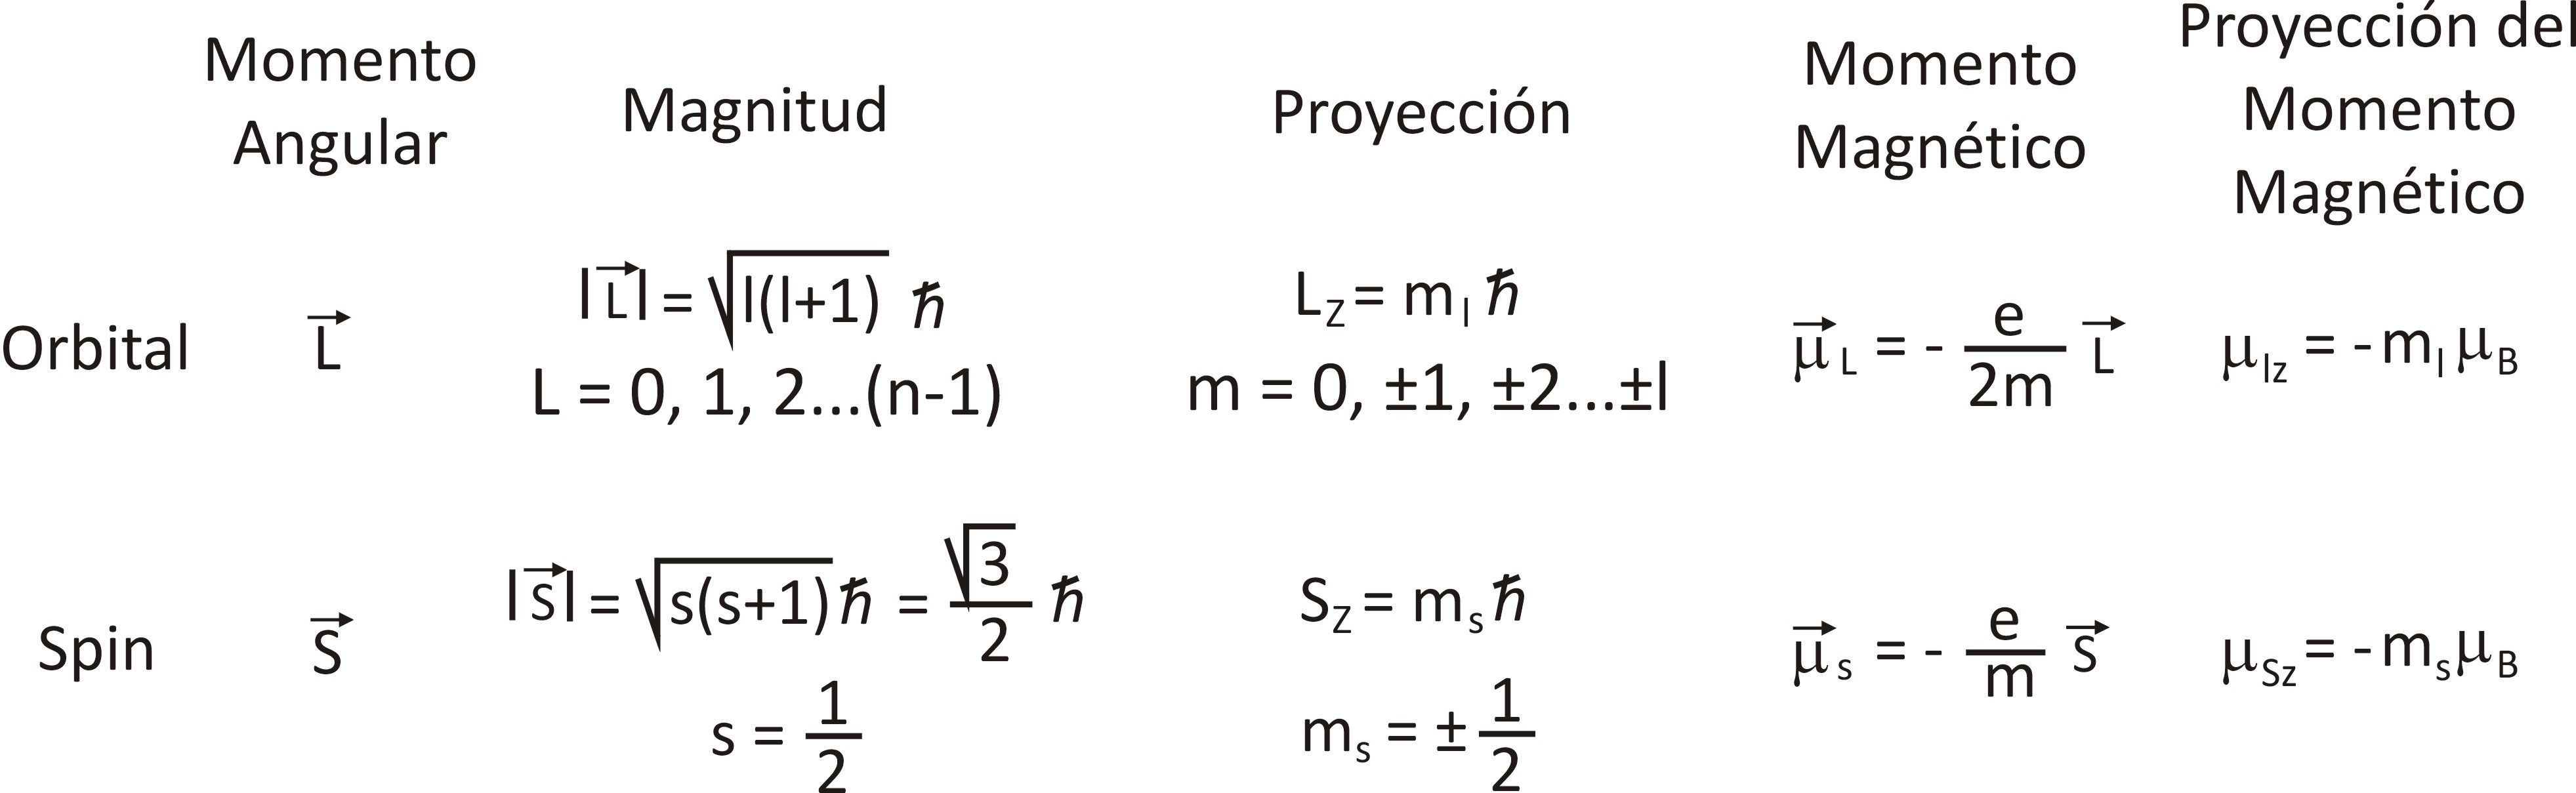
\includegraphics[width=1.0\textwidth]{./Figures/LyS}
	\caption{Resumen de números cuánticos}
	\label{fig:GraficoLyS}
\end{figure}

\textbf{Ejemplo:}

Calculemos los ángulos que forman $L_{z}$ y el vector $\overrightarrow{L}$, en nuestro caso $l = 2$


\begin{equation}
  sin \big(\alpha\big)=\frac{L_{z}}{|\V{L}|}=\frac{m_{l}\,\hbar}{\sqrt{l(l+1)} \, \hbar}=\begin{cases}
  				m_{l}=2 \rightarrow\alpha\approx 46^{\circ} \\
  				m_{l}=1 \rightarrow\alpha\approx 24^{\circ} \\  				
  				m_{l}=0 \rightarrow\alpha=0^{\circ} \\
  				m_{1}=-1 \rightarrow\alpha\approx 336^{\circ} (-24^{\circ})\\
  				m_{1}=-2 \rightarrow\alpha\approx 314^{\circ} (-46^{\circ})
    			\end{cases}
\end{equation}

El vector momento angular orbital nunca puede estar alineado al campo magnético, ya que ello requeriría que el ángulo $\alpha$ tomase un valor de $90^{\circ}$ o de $270^{\circ} (-90^{\circ})$, para lo cual se requeriría que:

\begin{equation}
 \frac{m_{l}}{\sqrt{6}}= \pm1 \quad \text{y por lo tanto} \quad m_{l}=\pm\sqrt{6}= \pm2,45
\end{equation}

Mayor que el valor $m_{l}\leq|2|$ en este caso. Por otro lado, si es coincidente con la dirección del campo conoceríamos las tres componentes de vector momento angular orbital, lo cual está prohibido.

Seguimos trabajando con el átomo de hidrogeno es decir con un solo electrón. Recordemos que el tratamiento que hacemos es semi cuántico. Cuando es posible, y si el resultado clásico no difiere mucho del cuántico utilizamos el modelo clásico.

\section{Interacción espín órbita L-S}

Vimos que un electrón en un átomo tiene un momento angular orbital $\V{L}$ y también un momento angular $\V{S}$ estos momentos pueden interactuar y acoplarse, se la llama interacción espín órbita (L-S) Luego, sumando vectorialmente los dos momentos se encuentra el momento angular total del átomo llamado $\V{J}$. No consideramos el momento angular del núcleo por ser varios miles de veces menor que la interacción L-S Luego, lo definimos como $\V{J}=\V{L}+\V{S}$. Este debe cumplir con las mismas propiedades que los momentos angulares $\V{L}$ y $\V{S}$.Es decir, debe ser ejecutado de acuerdo a los lineamientos de la mecánica cuántica La interacción L-S, es muy débil en el átomo de hidrógeno, pero muy importante en átomos con más electrones 

$\vert \V{J} \vert = \sqrt{J(J+1)}\hbar$, donde $J$ es el numero cuántico correspondiente.

En general $J$ varia desde $(l-s), (l-s+1), \cdots, (l+s-1), (l+s)$ luego para un electrón $\vert l-\dfrac{1}{2}\vert \leq j \leq \vert l+\dfrac{1}{2}\vert$ luego $j=l \pm \dfrac{1}{2}$. Mientras que $J_{z}=m_{j}\hbar$.
 
Analicemos como se puede realizar la suma e indaguemos si puede ser arbitrara el ángulo que forman los vectores. Para eso consideremos el siguiente esquema y aplicamos el teorema del coseno.

\begin{equation}
	J^{2}=L^{2}+S^{2}+2\,L\,S\,Cos(\alpha)
\end{equation}

Los módulos de los vectores se miden en unidades de $\hbar$, luego reemplazando los módulos:

\begin{equation}
	j(j+1)=l(l+1)+s(s+1)+2\,\sqrt{l(l+1)}\,\sqrt{s(s+1)}\,Cos(\alpha)
\end{equation}

Por lo tanto:

\begin{equation}
	Cos(\alpha) = \dfrac{j(j+1)-l(l+1)-s(s+1)}{2\,\sqrt{l(l+1)}\,\sqrt{s(s+1)}}
\end{equation}

Donde vemos que el valor del ángulo no puede ser cualquiera y depende de los números cuánticos $l$ y $s$ ya que el numero cuántico $j$ también depende de los anteriores. Se ve que para un valor fijo de $l$,  $j$ puede tomar solo dos valores $j=l \pm \dfrac{1}{2}$, luego hay solo dos valores del ángulo para cada $l$. Estos dos estados tiene una pequeña diferencia de energía y es lo que genera la llamada estructura fina de las líneas espectrales.

Veamos un ejemplo: 

Primero para $l=1$, $s=+\dfrac{1}{2}$. Calculamos los módulos de los vectores para $j=1+s=\dfrac{3}{2}$ luego construimos la suma conociendo los lados

\begin{equation*}
	\begin{aligned}[c]
		&\qa{j}=\dfrac{3}{2}\big(\dfrac{3}{2}+1\big)= \dfrac{15}{4}\\
		&\qa{l}=2\\
		&\qa{s}=\dfrac{3}{4}
	\end{aligned}
\qquad\Longrightarrow\qquad
	\begin{aligned}[c]
		&\lv{J} = \qa{j}=\sqrt{\dfrac{15}{4}}=1,90\\
		&\lv{L}=\qa{l}=\sqrt{2}=1,41\\
		&\lv{S}=\qa{sl}=\sqrt{\dfrac{3}{4}}=0,86
	\end{aligned}
\end{equation*}

Por el teorema del coseno podemos verificar que el ángulo es el correcto. Recordemos que todo se mide en unidades de $\hbar$

Ahora calculemos $l=1$, $s=-\dfrac{1}{2}$, los valores absolutos de $l$ y $s$ no cambian y ahora  hacemos el calculo con el teorema del coseno:

\begin{equation}
	\begin{aligned}[c]
	Cos(\alpha) =& \dfrac{j(j+1)-l(l+1)-s(s+1)}{2\,\sqrt{l(l+1)}\,\sqrt{s(s+1)}} = \dfrac{\qa{\dfrac{1}{2}}-2-\dfrac{3}{4}}{2\sqrt{2}\sqrt{\dfrac{3}{4}}}=\\
	&\dfrac{-2}{2,44}=-0,81\Rightarrow \alpha = 143^{o}
	\end{aligned}
\end{equation}


mientras que el modulo de $\lv{J}$ es igual a $\qa{l}=\qa{\dfrac{1}{2}}=\sqrt{\dfrac{3}{4}}=0,86$ tal como se ve representado en la figura \ref{fig:115}. Vemos que si el átomo tiene un solo electrón hay solo dos orientaciones posibles: en la primera $\lv{J}>\lv{L}$ mientras que en la segunda $\lv{J}<\lv{L}$.


\begin{figure}[H]
    \centering
    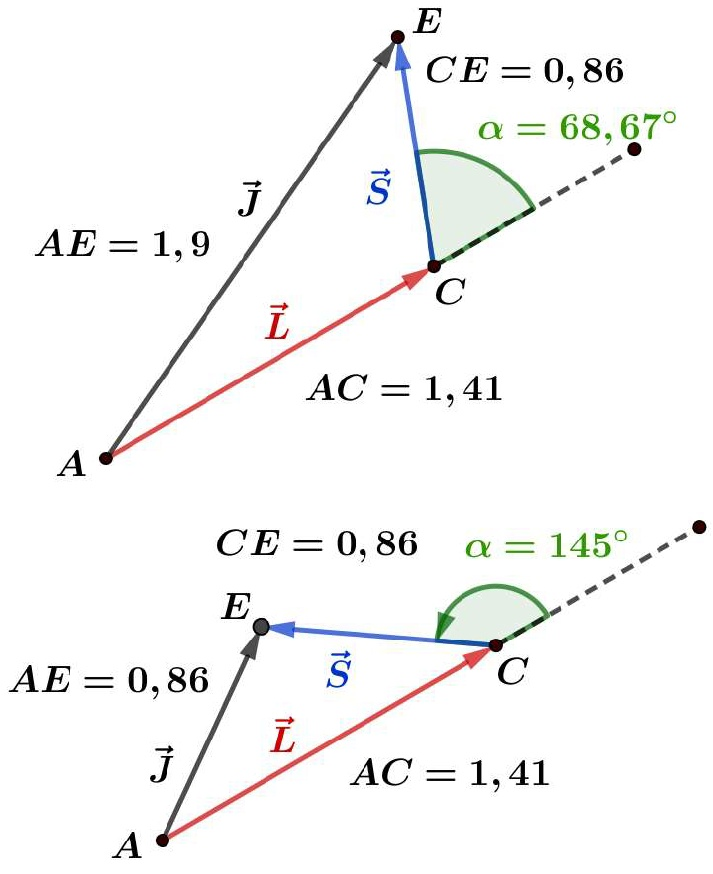
\includegraphics[width=0.6\textwidth]{./Figures/fig115}
	\caption{Interacción L-S}
	\label{fig:115}
 \end{figure}

En ausencia de campo magnético externo, el momento angular total del átomo $\V{J}$ se conserva, es decir modulo y dirección constante, en tanto $\V{L}$ y $\V{S}$ rotaran al rededor de $\V{J}$. Por supuesto, para el átomo de hidrógeno con un solo electrón.

Si ahora aplicamos un campo $\V{B}$ exterior débil, de manera que no rompa la interacción espín orbita (L-S) Sera $\V{J}$ quien rote alrededor del campo eterno sin romper la iteración (L-S), luego seguirán rotando $\V{L}$ y $\V{S}$ alrededor de $\V{J}$ La orientación de $\V{J}$ en el campo externo $\V{B}$  deberá cumplir con uno de los valores permitidos de $m_{j}$ Si se aumenta el campo magnético externo se rompe el acoplamiento (L-S) y dejan $\V{L}$ y $\V{S}$ de rotar alrededor de $\V{J}$. Observe la figura \ref{fig:116} 


\begin{figure}[H]
    \centering
    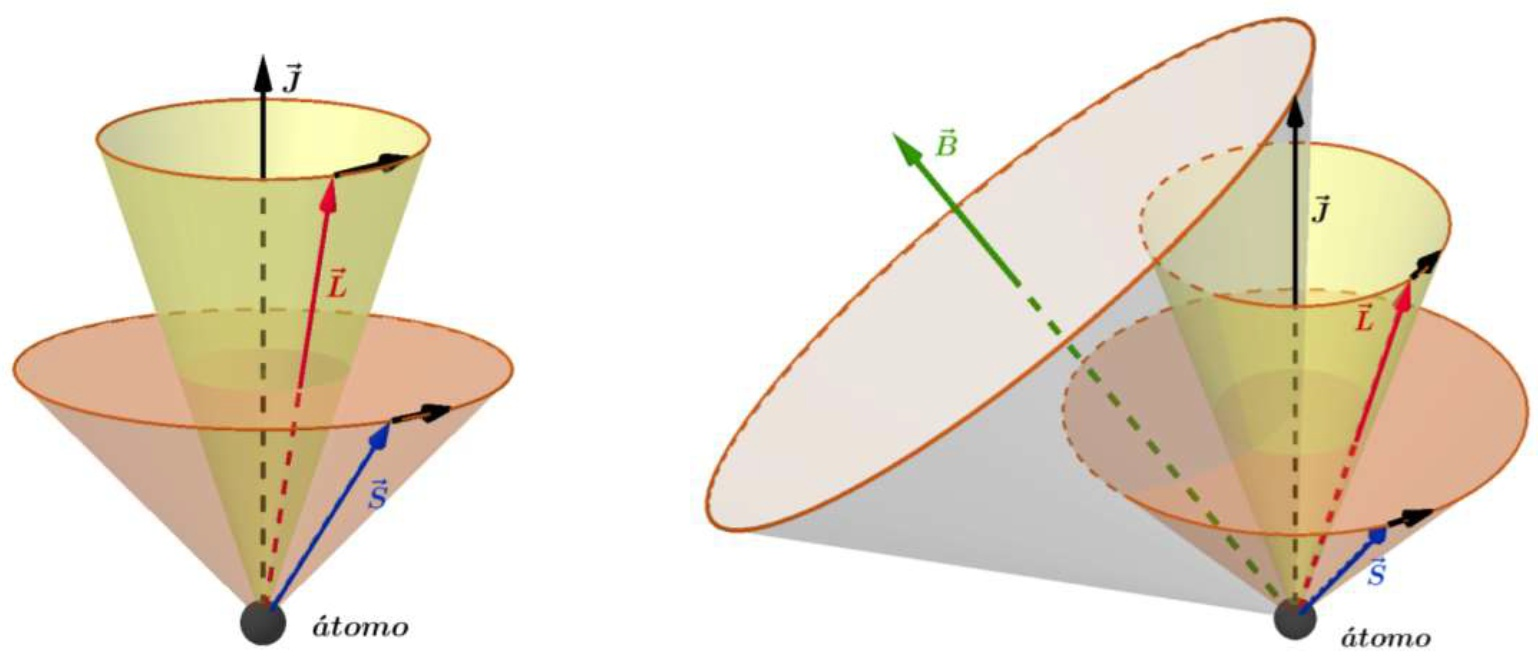
\includegraphics[width=1.0\textwidth]{./Figures/fig116}
	\caption{Interacción L-S}
	\label{fig:116}
 \end{figure}


\section{Momento magnético total de un átomo libre}

El momento magnético efectivo del átomo seria la suma de las componentes $\V{\mu_{L}}$ y $\V{\mu_{S}}$ Calculemos las suma de los momentos magnético que llamamos $\V{\mu_{total}}$

\begin{sloppypar}
\begin{equation}
	\V{\mu}_{total}=\V{\mu}_{L}+\V{\mu}_{S}=-\mu_{B}(\V{L}+g\V{S})=-\mu_{B}(\V{L}+2\V{S})=-\mu_{B}(\V{J}+\V{S})
\end{equation}

Esta expresión nos indica que $\mu_{total}$ es directamente opuesto a $\V{J}$, salvo que ${\V{S}=0}$, $\V{\mu}_{total}$ también girará alrededor de $\V{J}$. La componente de $\mu_{total}$ en la dirección de $\V{J}$ es $\V{\mu_{j}}$ Como se observa en la figura \ref{fig:117}, en la cual no se respetaron las longitudes relativas de los vectores.

\begin{figure}[H]
    \centering
    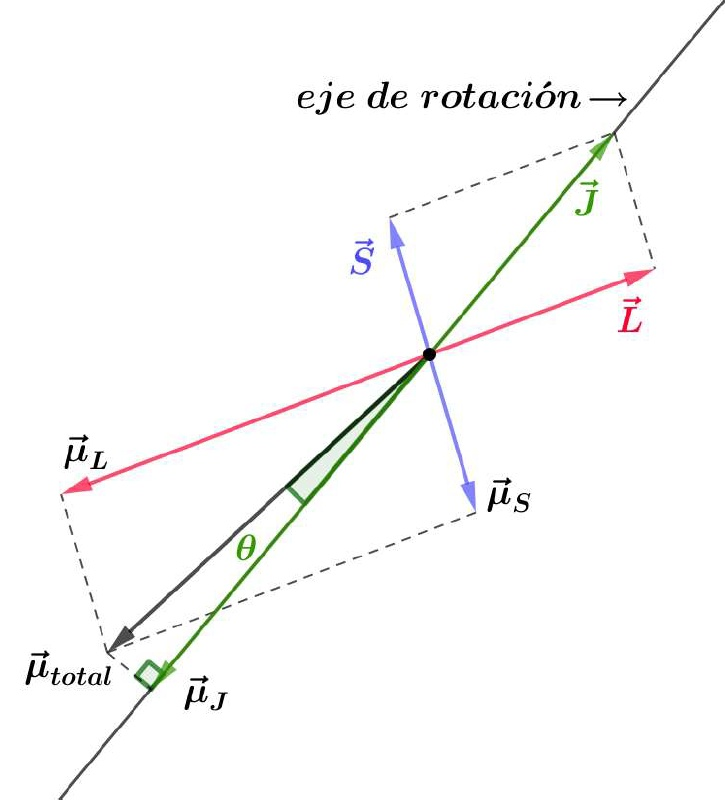
\includegraphics[width=0.7\textwidth]{./Figures/fig117}
	\caption{Momento magnético total de un átomo libre II}
	\label{fig:117}
 \end{figure}

\end{sloppypar}


\begin{itemize}


\item Anteriormente se vio que el momento angular orbital y de espín se sumaban formando el momento magnético atómico total El momento magnético total de un átomo libre tiene tres contribuciones el momento magnético del núcleo, el momento magnético orbital más el momento magnético del electrón

\item El núcleo atómico tiene carga y presenta momento magnético, este eses103veces inferior a los generados por los electrones, luego, \textbf{no se considera el momento magnético nuclear}.

\item Luego en un átomo, el campo magnético observado es debido al acoplamiento de estos dos momentos: \textbf{orbital y del espín}. 
\end{itemize}

Como sabemos el momento angular total $\V{J}$ es la suma del momento del spin $\V{S}$ con el orbital $\V{L}$. El momento magnético en la dirección $\hat{J}$ será:

\begin{equation}
	\mu_{j}=\lv{\mu_{j}}=\lv{\mu_{l}}Cos(\beta)+\lv{\mu_{s}}Cos(\alpha)
\end{equation}

Donde el ángulo $\hat{SJ}= \alpha$ y el ángulo $\hat{LJ}=\beta$, reemplazando y operando se llega a:

\begin{equation*}
	\mu_{j}=g_{j}\mu_{B}\sqrt{\qa{j}} \quad \text{con } g_{j} \text{ factor de Landé para } j \text{que vale: }
\end{equation*}

\begin{equation*}
	g_{j}= 1 +\dfrac{\qa{l}+\qa{s}-\qa{l}}{2\qa{j}} \quad \text{como veremos seguidamente}
\end{equation*}

Como sabemos el $\mu_{total}$ no esta en la dirección de $\V{J}$ y recordando que $\V{L}$ y $\V{S}$ rotan alrededor de $\V{J}$, luego $\V{\mu}_{L}$ y $\V{L}_{S}$  también rotal alrededor de $\V{J}$. En el esquema se observa la distribución espacial de los mismos Luego si pretendemos sumarlos es adecuado descomponer $\V{\mu}_{S}$ y $\V{\mu}_{S}$ en dos componentes, una en la dirección del eje de rotación y la otra perpendicular al mismo, esta ultima, como rota, tendrá valor medio cero Por el contrario, si tendrá un valor determinado distinto de cero, aquellas que proyectamos en la dirección del eje de rotación.


\begin{figure}[H]
    \centering
    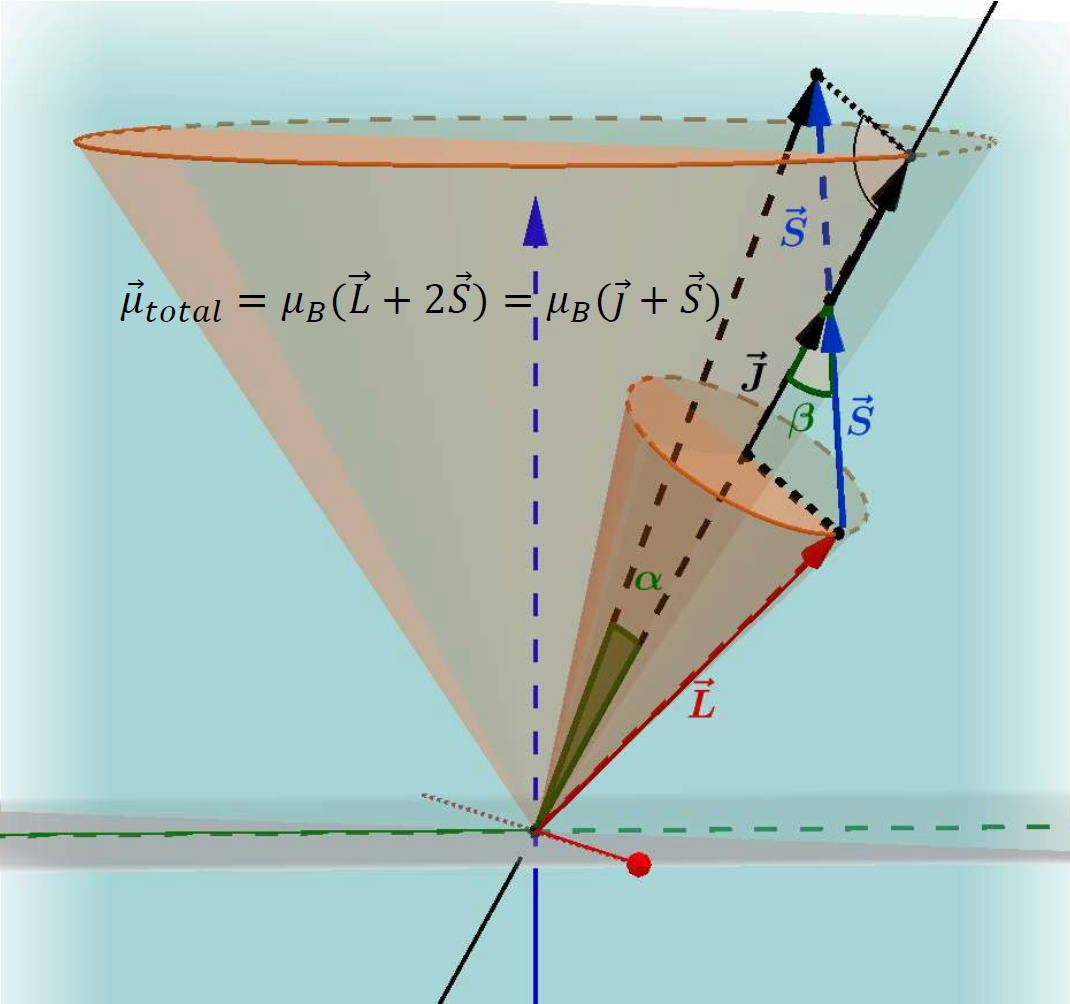
\includegraphics[width=0.9\textwidth]{./Figures/fig118}
	\caption{Momento magnético total de un átomo libre II}
	\label{fig:118}
 \end{figure}

En la figura \ref{fig:119} se observan los ángulos que se utilizaran en el desarrollo de $G_{e}$ como veremos a continuación

\begin{figure}[H]
    \centering
    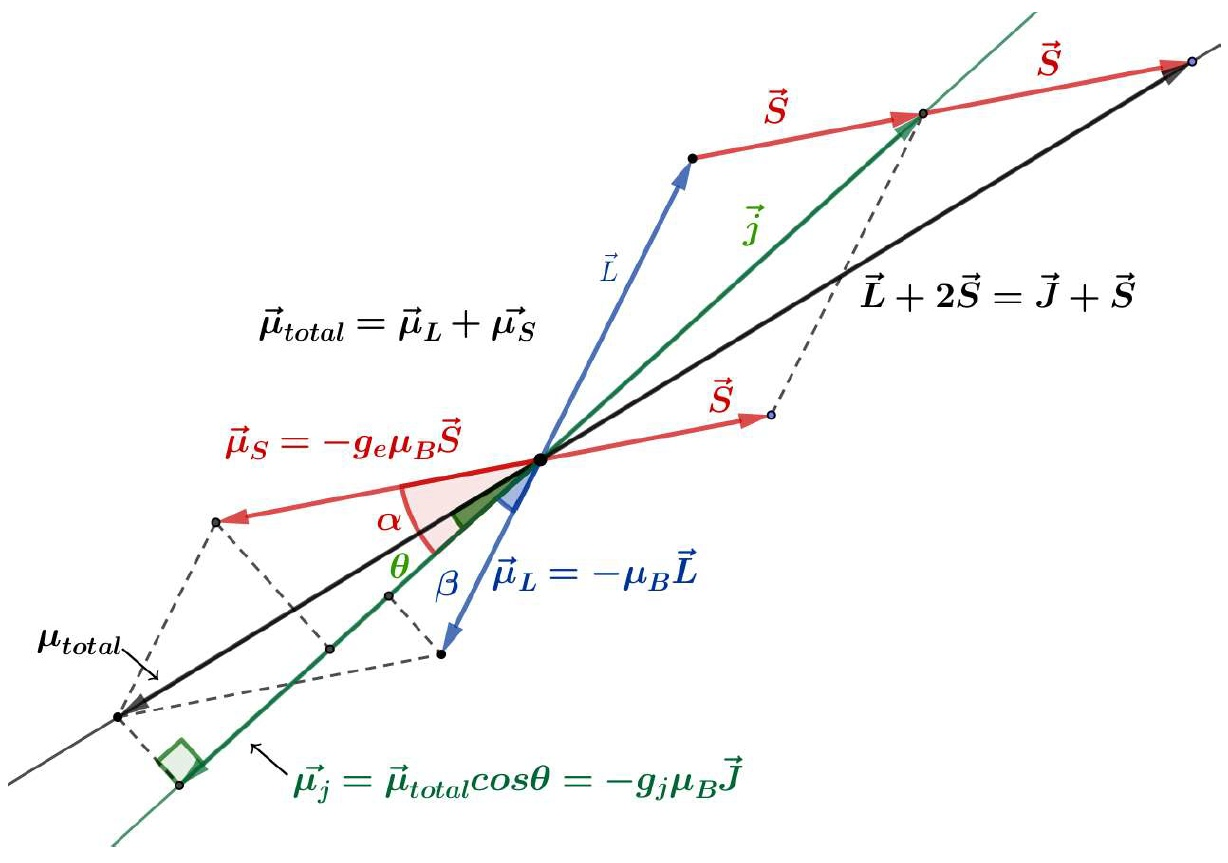
\includegraphics[width=1.0\textwidth]{./Figures/fig119}
	\caption{Momento magnético total de un átomo libre III}
	\label{fig:119}
 \end{figure}
 
Dijimos que:
 
\begin{equation*}
	\mu_{j}=\lv{\mu_{j}}=\lv{\mu_{l}}Cos(\beta)+\lv{\mu_{s}}Cos(\alpha)
\end{equation*} 

y por el teorema del coseno:

\begin{equation*}
	\begin{aligned}[c]
	&\lv{S}^{2}=\lv{L}^{2}+\lv{J}^{2}-2\lv{L}\lv{J}Cos(\beta)\therefore \\
	&Cos(\beta)=\dfrac{\lv{L}^{2}+\lv{J}^{2}-\lv{S}^{2}}{2\lv{L}\lv{J}}= \dfrac{\qa{l}+\qa{j}-\qa{s}}{2\sqrt{\qa{l}\qa{j}}}
	\end{aligned}
\end{equation*} 

De igual manera procedemos para el otro triangulo:

\begin{equation*}
Cos(\alpha)= \dfrac{\qa{s}+\qa{j}-\qa{l}}{2\sqrt{\qa{s}\qa{j}}}
\end{equation*} 

Remplazando los cosenos en la ecuación:

\begin{equation*}
	\begin{aligned}[c]
	&\lv{\mu_{j}}=\lv{\mu_{l}}Cos(\beta)+\lv{\mu_{s}}Cos(\alpha) \\
	&\lv{\mu_{j}}=\lv{\mu_{l}}\dfrac{\qa{l}+\qa{j}-\qa{s}}{2\sqrt{\qa{l}\qa{j}}}+\lv{\mu_{s}}\dfrac{\qa{s}+\qa{j}-\qa{l}}{2\sqrt{\qa{s}\qa{j}}} \\
	&\lv{\mu_{j}}=\mu_{B}\left[\lv{L} \dfrac{\qa{l}+\qa{j}-\qa{s}}{2\sqrt{\qa{l}\qa{j}}}+2\lv{S}\dfrac{\qa{s}+\qa{j}-\qa{l}}{2\sqrt{\qa{s}\qa{j}}}\right] \\ 
	&\lv{\mu_{j}}=\mu_{B}\left[ \dfrac{\qa{l}+\qa{j}-\qa{s}}{2\sqrt{\qa{j}}}+2\dfrac{\qa{s}+\qa{j}-\qa{l}}{2\sqrt{\qa{j}}}\right] \\
	&\lv{\mu_{j}}=\mu_{B}\left[ \dfrac{3\qa{j}+\qa{s}-\qa{l}}{2\sqrt{\qa{j}}} \right] \\
	&\lv{\mu_{j}}=\mu_{B}\left[ \dfrac{3\qa{j}+\qa{s}-\qa{l}}{2\qa{j}} \right]\sqrt{ \qa{j}} \\	
	&\lv{\mu_{j}}=\mu_{B}\left[1+ \dfrac{\qa{j}+\qa{s}-\qa{l}}{2\qa{j}} \right]\sqrt{\qa{j}} \\	
	&\lv{\mu_{j}}=\mu_{B}\,g_{j}\,\sqrt{\qa{j}}\quad \text{o bien: } \quad \V{\mu}_{j}=\mu_{B}\,g_{j}\,\V{L} 	
	\end{aligned}
\end{equation*} 



\section{Átomos con más de un electrón}
Hemos avanzado bastante con el magnetismo atómico nos faltaría generalizar las ideas a átomos con más de un electrón Los átomos que nos interesa desde el punto de vista del magnetismo son llamados elementos de transición y poseen gran cantidad de electrones No se puede resolver teóricamente el sistema de varios cuerpos, ni siquiera en mecánica clásica Sin embargo es posible, con las ideas expuestas anteriormente, comprender y explicar varios fenómenos de átomos con varios electrones. O sea el estado del electrón en el átomo lo determinan cuatro números cuánticos.


Visto lo expuesto, podríamos preguntarnos:

\textbf{¿Cómo se distribuyen los electrones en los átomos dando origen a los distintos elementos químicos que conforman la tabla periódica?}

Analicemos lo que ya sabemos:

\begin{itemize}
	\item El movimiento de pequeñas partículas (electrones, neutrones, etc.) en una zona limitada del espacio, (pozo de potencial, átomo, molécula) está determinado por parámetros adimensionales llamados números cuánticos, estos pueden tomar determinados valores. La cantidad de números cuánticos necesarios en la solución de un problema depende del número de grados de libertad de la partícula, (pozo de potencial uní dimensional un número cuántico, si el pozo es tridimensional serán tres los números). Si además la partícula puede girar sobre si misma tendremos un número cuántico más.
	\item A distintos valores de los número cuánticos corresponde diferentes energías, luego hay niveles discretos de energía. La partícula no puede tener cualquier energía.
	\item Recordemos que lo mencionada hasta aquí se encuentra justificado experimentalmente y teóricamente. Al resolver el problema del movimiento de un electrón en un átomo en el espacio es necesario introducir tres números cuánticos: $n, l, m_{l}$.
	\item  \textcolor{red}{\textbf{n: Número cuántico principal}} vale 1,2,3….define el tamaño de las orbitas, es el que tiene mayor influencia en la energía, cuando mayor sea mayor será el volumen. Siendo $K (n=1), L(n=2)$.
	\item \textcolor{red}{\textbf{l: Número cuántico del momento angular}} indica la forma del orbital y el momento angular, toma vale $0 ,1, 2,.. (n -1)$. Designando $l=0$ como $s$, $l=1$ como $p$, $l=3$ como $d$, etc.
	\item  \textcolor{red}{\textbf{$\boldsymbol{m_{l}}$: Número cuántico magnético}} define la orientación espacial del orbital frente a un campo magnético externo, toma valores $-l,..,0,..,l$.
	\item \textcolor{red}{\textbf{$\boldsymbol{m_{s}}$: Numero cuántico de espín}} Por último es necesario introducir un cuarto numero cuántico no previsto por la mecánica clásica, el número cuántico de espín toma valores $-\frac{1}{2}$ y $+\frac{1}{2}$ para indicar las dos orientaciones del electrón.
\end{itemize}

Para poder realizar el llenado de las capas electrónicas\footnote{El nombre de Capa Electrónica se deriva del modelo de Bohr, en el cual se postulaba que los grupos de electrones orbitaban el núcleo a ciertas distancias, así que sus órbitas formaban capas alrededor de los núcleos. Las capas electrónicas son numeradas correlativamente, partiendo de la más cercana al núcleo, y se identifican mediante letras: n = 1 capa K, n = 2 capa L, n = 3 capa M,...., n = 7 capa Q,} que se corresponden a cada número cuántico principal n de todos los elementos, debemos introducir algunas ideas más.

\begin{itemize}
	\item \textbf{Principio de Pauli}: en un átomo no puede haber dos electrones con los cuatro números cuánticos iguales.
	
Ya comentamos que en la mecánica clásica y en la cuántica las partículas admiten comportamientos
totalmente distinto En mecánica clásica las partícula se mueven en trayectorias bien determinadas, de
tal manera que podemos distinguir una de otra y saber en que instante se encontrara en una dada
posición En cuántica es totalmente distinta la situación Las partícula idénticas son totalmente
indistinguibles Esto quiere decir, de otra forma, que si en cuántica cambio una partícula por otra igual el estado cuántico no debe modificarse Si indicamos con $\Psi(1,2)$ la función de onda de un sistema donde $1$ y $2$ son las coordenadas de la primera y segunda partícula. Si intercambiamos las posiciones de las partículas el sistema sigue descripto por la misma función de onda, al menos multiplicada por una constante $\varepsilon$

\begin{equation*}
	\Psi(1,2)=\varepsilon\Psi(2,1)
\end{equation*}

El valor de $\varepsilon$ viene determinado solo por el tipo de partícula, puede tomar solo dos valores $\varepsilon=+1$ o $\varepsilon=-1$ 

Todas las partículas con espín nulo o entero son llamadas Bosones y cumplen con que:

\begin{equation*}
	\Psi(1,2)=+\Psi(2,1)
\end{equation*}


todas las partículas que tienen spin semientero son llamadad Fermiones y cumplen con que:

\begin{equation*}
	\Psi(1,2)=-\Psi(2,1)
\end{equation*}

Los electrones son Fermiones La mecánica cuántica impone estrictas leyes sociales (cuando interactúan entre ellas) Por ejemplo los Fermiones en sociedad deben cumplir que no pueden haber dos de ellos ( en un átomo con el mismo conjunto número cuántico. Esto es el principio de Pauli y fue demostrado a posteriori. Como vemos los fermiones son entes ermitaños, no les gustan sus semejantes, sin embargo son todos iguales, indistinguibles.	
	
	\item \textbf{Regla de Hund\footnote{Reglas de Hund: El estado fundamental de un átomo (estado de más baja energía)viene determinado por la combinación de los números cuánticos de los electrones individuales de la capa incompleta, de acuerdo con un conjunto de instrucciones denominadas reglas de Hund que proporcionan el nº cuántico compuesto J correspondiente al estado fundamental:
\begin{itemize}	
\item[1] Los spines de los electrones se distribuyen de tal manera que exista el mayor número de spines paralelos sin que se viole el principio de Pauli. Haciendo $s = +1/2$ ó $-1/24$ se calcula $Sc$ \textbf{momento angular de espín combinado}.
\item[2] Los electrones con espines combinados según 1. se distribuyen entre los posibles valores de $ml$ de manera que $Sml = Lc$ sea máxima. $Lc$ es el \textbf{momento angular orbital combinado}.
\item[3] Los estados de un átomo, caracterizados por su \textbf{momento angular total $J$}, vienen dados por un número cuántico $J$ que toma valores enteros desde $|Lc - Sc|$ hasta $|Lc + Sc|$. El estado fundamental viene dado por $J = |Lc - Sc|$ para una capa llena hasta menos de la mitad, y $J= |Lc + Sc|$ para una capa llena hasta más de la mitad.
\end{itemize}}}: Al llenar orbitales, los tres $p$, los cinco $d$ o los siete $f$ , de igual capa nivel de energía o capa n, los electrones se distribuyen, siempre que sea posible, con sus espines paralelos (apuntando en la misma dirección), ya que la partícula es más estable (tiene menos energía) cuando tiene electrones desapareados (espines paralelos) que cuando esos electrones están apareados (espines opuestos o antiparalelos)
\end{itemize}

Podemos imaginar que los átomos que constituyen la tabla periódica se van formando agregando electrones, estos crean nuevos orbítales una vez que se llenan los primeros. O sea si $n=1$ y $l=0$ es la primer capa que se llena con dos electrones, $n=2$ tenemos dos sub capas una para $n=1$ y $l=0$ estamos en el caso anterior, si $l=1$ tenemos dos subcapas, en total 8 electrones, siguiendo de esta manera obtenemos todos los átomos de la tabla periódica. La repetición de $l$ corresponde a  propiedades químicas similares, luego los átomos que tengan en su ultima capa un solo electrón en la subcapa $s$ tienen propiedades similares. Veamos algunos elementos y sus estructuras electrónicas $H= 1S^{1}, \; He=1s^{2}, \; Li=1s^{2}2s_{1}, \; Be=1s^{2}2s_{2}$


\begin{figure}[H]
    \centering
    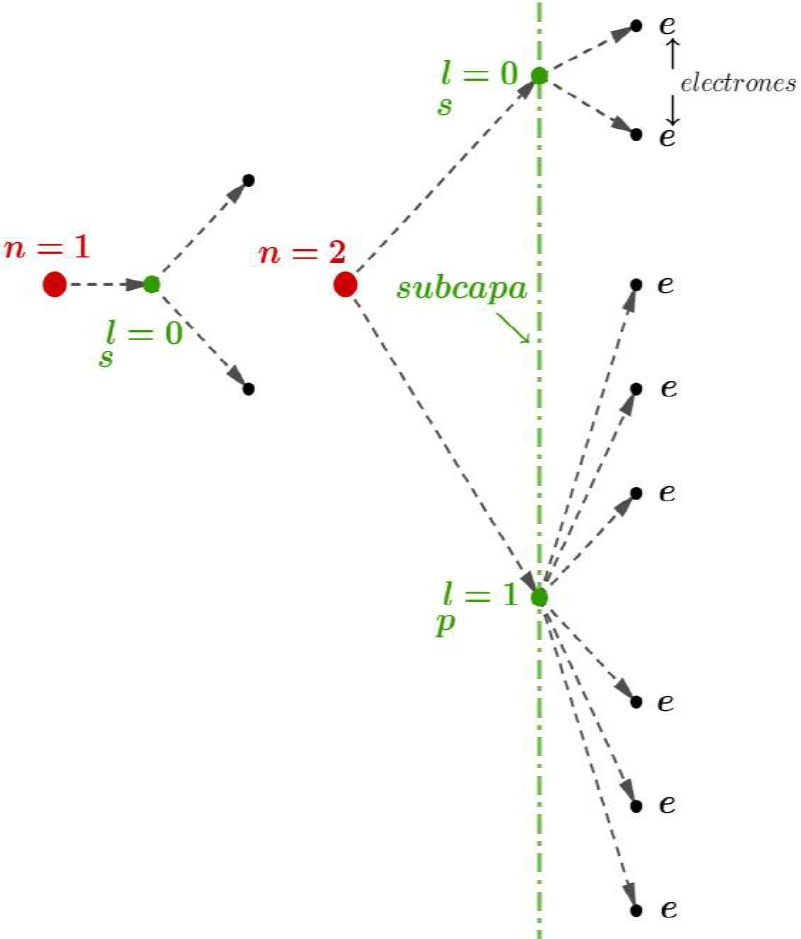
\includegraphics[width=0.8\textwidth]{./Figures/fig120}
	\caption{Distribución de fermiones $e^{-}$}
	\label{fig:120}
 \end{figure}


Los electrones deben cumplir una serie de condiciones para ser introducidos al átomo Para ello debemos desarrollar la regla empírica de Friedrich Hund presentado en 1927 o de máxima multiplicidad, la cual nos indica como ubicar los electrones Al llenar orbitales, de igual energía, los electrones se distribuyen, siempre que sea posible, con sus espines paralelos (apuntando en la misma dirección), ya que la partícula es más estable cuando tiene electrones desapareados (spines paralelos) que cuando esos electrones están apareados (spines opuestos o antiparalelos) Dicho de otro modo, se introducen los electrones de tal manera que ocupen primeramente las regiones del átomo donde la probabilidad de encontrarlos en el espacio es mayor Veamos en el esquema un caso real y otro imposible Existen varias reglas para ir llenando los orbitales, regla de \textit{Aufbau} es una de ellas. La palabra \textit{aufbau} se refiere al verbo alemán “construir“ no es el nombre de ningún científico

\begin{figure}[H]
    \centering
    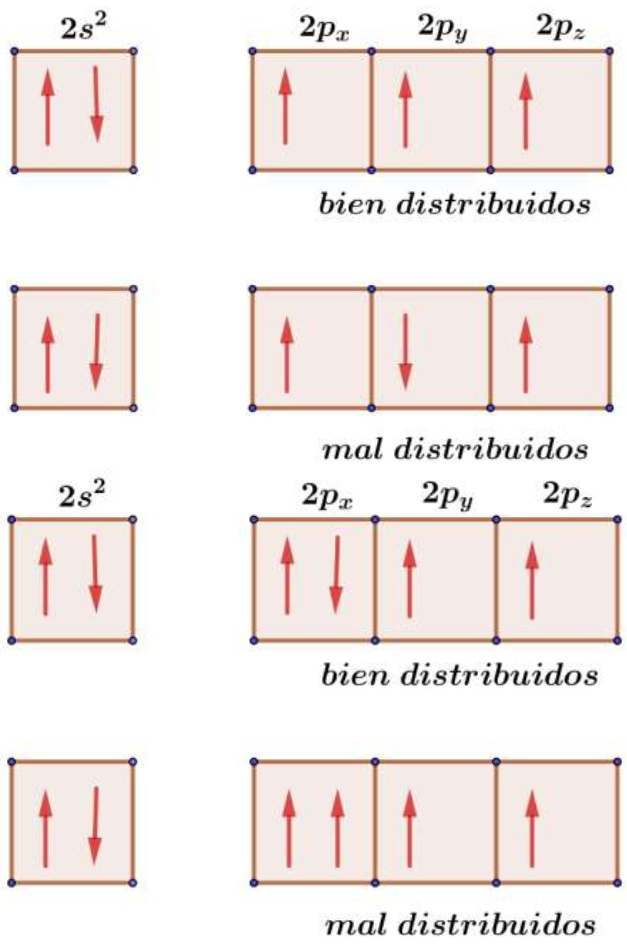
\includegraphics[width=0.4\textwidth]{./Figures/fig121}
	\caption{Distribución siguiendo la regla de Hund}
	\label{fig:121}
 \end{figure}

Al ir agregando electrones obtenemos la tabla periódica de los elementos. Vemos que el primer grupo se inicia con el $H$ y finaliza con $He$ que llena la capa $1s$ con dos electrones y es noble. Luego, el siguiente nivel $n$ comienza con el $Li$ se llena la capa $2s$ con el $Be$ y se completa la acapa $2p$ con el $Ne$ que también es noble. La capa siguiente es similar. Podemos verlo en la figura \ref{fig:122}


\begin{figure}[H]
    \centering
    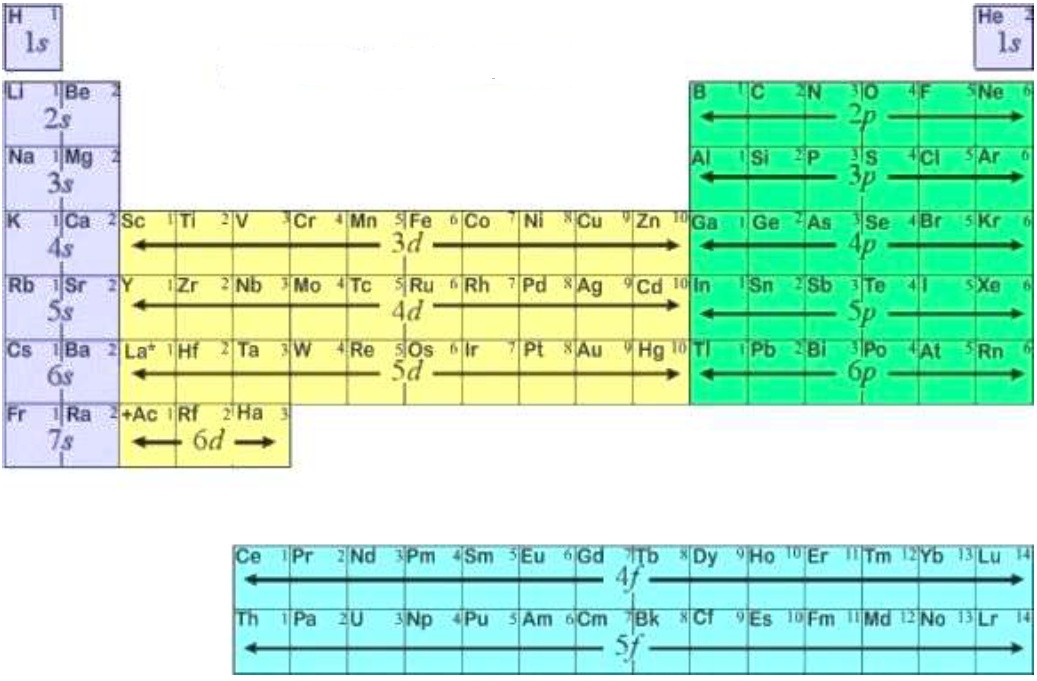
\includegraphics[width=1.0\textwidth]{./Figures/fig122}
	\caption{Capas $n$ y orbitales $l$}
	\label{fig:122}
 \end{figure}

Si los electrones llenan por completa la capa $n$ o $l$ prefijada, tienen momento orbital total y de espín nulo, por ejemplo los gases inertes $He,\; Ne,\; Ar,\; Kr,\; Xe\; \text{y}\; Rn$  La mayoría de los átomos tienen un momento magnético distinto de cero como podemos ver en la tabla de la figura \ref{fig:GraficoAlineaciónDelSpin}


\begin{figure}[H]
    \centering
    \includegraphics[width=1.0\textwidth]{./Figures/AlineaciónDelSpin}
	\caption{Alineación de los espines electrónicos}
	\label{fig:GraficoAlineaciónDelSpin}
\end{figure}


\textbf{Recordando algo de química:}

Cada capa se compone de una o más subcapas, que a su vez se componen de los orbitales atómicos. Por ejemplo, la primera capa ($K$) tiene una subcapa, llamada $1s$; la segunda capa ($L$) tiene dos subniveles, llamados $2s$ y $2p$; la tercera capa ($M$) tiene $3s$, $3p$ y $3d$; la cuarta ($N$) tiene las subcapas $4s$, $4p$, $4d4 y $4f4; la quinta capa ($O$) tiene $5s$, $5p$, $5d$ y $5f$ etc.

\begin{figure}[H]
    \centering
    \includegraphics[width=0.6\textwidth]{./Figures/Gráfico5}
	\caption{Llenado de los orbitales,}
	\label{fig:Grafico5}
\end{figure}

en la figura \ref{fig:Grafico5} podemos observar que de $3p$ se pasa a $4s$. El potasio comienza a llenar la $4s$, sin haber completado la $3d$.

El número cuántico $l$ determina la excentricidad de la órbita, cuando mayor sea, más excéntrica será.
Así para todos los $l=0$ ($1s$, $2s$, $3s$, etc.) independientemente de la capa, tendremos un orbital esférico.

\begin{figure}[H]
    \centering
    \includegraphics[width=0.6\textwidth]{./Figures/1S2S3S}
	\caption{orbitales esféricos de las capas s}
	\label{fig:Grafico1s2s3s}
\end{figure}

A partir de la capa $L (n=2)$, corresponderá además de $l=0$, $l= 1$ ($2p$, $3p$, $4p$, etc.)


\begin{figure}[H]
    \centering
    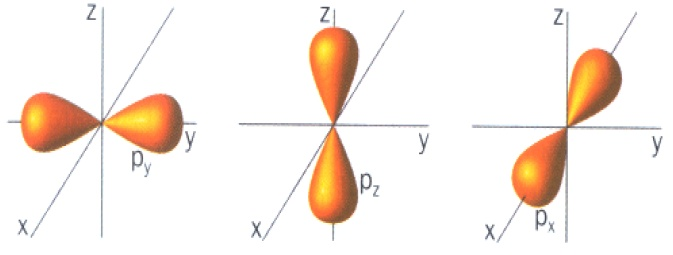
\includegraphics[width=0.8\textwidth]{./Figures/OrbitalesP}
	\caption{orbitales p}
	\label{fig:GraficoOrbitalesP}
\end{figure}

\begin{figure}[H]
    \centering
    \includegraphics[width=0.6\textwidth]{./Figures/Gráfico7}
	\caption{orbitales l}
	\label{fig:Grafico7}
\end{figure}

Podemos ver como se acomodan las primeras capas y orbitales:

\begin{figure}[H]
    \centering
    \includegraphics[width=0.7\textwidth]{./Figures/variosOrbitales}
	\caption{orbitales sucesivos}
	\label{fig:variosOrbitales}
\end{figure}

Con la capa $M$ ($n=3$) comienzan los orbitales $d$, $l=2$: $3d$, $4d$, $5d$, etc.

\begin{figure}[H]
    \centering
    \includegraphics[width=0.8\textwidth]{./Figures/Gráfico8}
	\caption{orbitales d}
	\label{fig:Grafico8}
\end{figure}


\subsubsection{Paramagnetismo y enlace iónico}

\begin{itemize}
	\item En general hemos hablado hasta ahora, de momentos magnéticos de átomos aislados, sabiendo que la gran mayoría de los átomos tienen momento magnético diferente de cero en comparación con los que tienen momento magnético cero. Pero la generalidad de los cuerpos están formados por moléculas y esto cambia la cosa, resultando mayor el número de sustancias solamente diamagnéticas, por el contrario, las moléculas paramagnéticas escasean. Veamos un caso que al combinarse átomos paramagnéticos para formar un sólido este resulta no ser paramagnético.
	\item La configuración electrónica del sodio es:\\
	\begin{equation}
		Na: 1s^{2} 2s^{2} 2p^{6} 3s^{1}  = [Ne]3s^{1}	
	\end{equation}		
mientras que para el cloro es:
	\begin{equation}
	Cl: 1s^{2} 2s^{2} 2p^{6} 3s^{2} 3p^{5}  = [Ne]3s^{2} 3p^{5}
	\end{equation}
	
vemos que para tener una estructura más estable, al sodio le sobraría un electrón y al cloro le faltaría uno. También vemos que ambos son paramagnéticos. Luego cuando se forma el $ClNa$, se crea el ion $Na^{+}$ pareciéndose al $Ne$ y el ion $Cl^{-}$ con electrónica análoga al $Ar$, por tanto debido a esta unión el compuesto $ClNa$ no es paramagnético.
\end{itemize}





\subsection{Suma de momentos angulares o momento angular total}

Habiamos visto para el átomo con un solo electrón que podíamos suponer que los dos momento angulares, el orbital y el de espín, si bien distintos, interactuaban acoplándose, dando origen al momento angular total del átomo (sin el núcleo) que llamamos $\V{J}$ y definimos como $\V{J}=\V{L}+\V{S}$, que debe cumplir las mismas propiedades que los momentos angulares $\V{L}$ y $\V{S}$. Es decir debe ser realizado de acuerdo a los lineamientos de la mecánica cuántica. Este tema suele introducirce como la suma de dos vectores cuantizados $\V{J_{1}}$ y $\V{J_{2}}$. para dar de esta manera generalidad al método. Luego tendremos:


\begin{equation}
	\mid\V{J_{1}}\mid =\sqrt{j_{1}\big(j_{1}+1\big)}\,\hbar \quad \text{con} \quad j_{1z}= m_{1}\hbar \quad \text{y} \quad -j_{1} \leq m_{1} \leq j_{1}
\end{equation}

\begin{equation}
	\mid\V{J_{2}}\mid =\sqrt{j_{2}\big(j_{2}+1\big)}\,\hbar \quad \text{con} \quad j_{2z}= m_{2}\hbar \quad \text{y} \quad -j_{2} \leq m_{2} \leq j_{2}
\end{equation}

%

Donde $jJ_{1}$ y $j_{2}$ son los números cuánticos correspondientes pudiendo ser enteros o semi enteros

\begin{equation}
	j_{1} \quad \text{y} \quad j_{2} \; \in \; \lbrace 0,\, \frac{1}{2},\, 1,\, \frac{3}{2},\, 2,\, \ldots\, \rbrace
\end{equation}

También $\V{J}=\V{L}+\V{S}$ deberá cumplir con las condiciones que impone la mecánica cuántica a los momento angulares, es decir:

\begin{equation}
	\mid\V{J}\mid =\sqrt{j\big(j+1\big)}\,\hbar \quad \text{con} \quad j_{z}= m\hbar \quad \text{y} \quad -j \leq m \leq j
\end{equation}

El número cuántico del momento angular total puede variar en pasos de a uno entre:

\begin{equation}
	\mid j_{1}-j_{2} \mid \leq j \leq \mid j_{1}+j_{2} \mid
\end{equation}

\subsection{Momento angular total de un átomo}

\begin{itemize}
	\item \textbf{Ejemplo:} suponemos que $\V{J_{1}}=\V{L}$  y $\V{J_{2}}=\V{S}$ , luego $\V{J}=\V{L}+\V{S}$ , como vimos $j$ varia entre $\mid j_{1}-j_{2} \mid \leq j \leq \mid j_{1}+j_{2} \mid$ o sea $\mid l-\frac{1}{2} \mid \leq j \leq \mid l+\frac{1}{2} \mid$, luego $j=l\pm\frac{1}{2}$.
	\item Si $l=0$ entonces $j=\frac{1}{2}$ (estado $s$ se designa $s_{\frac{1}{2}}$).	
	\item Si $l=1$ entonces $j=\frac{1}{2}; j=\frac{3}{2}$ (estado $p$ se designa $p_{\frac{1}{2}}; p_{\frac{3}{2}}$).
	\item Podemos tener una imagen del fenómeno pensando que la suma se realiza de manera clásica, pero, no es tan así. Clásicamente para sumarlos deberíamos conocer el ángulo que forman los vectores y sus módulos, luego aplicar el teorema del coseno.
	\item Sigamos con el ejemplo: vimos que para el caso en que $l\neq0$ el momento angular total $J=l\pm\frac{1}{2}$, calculemos el modulo de $\mid\V{J}\mid =\sqrt{j\big(j+1\big)}\,\hbar$ para los dos casos del número cuántico $j$ del momento angular total


\begin{figure}[H]
    \centering
    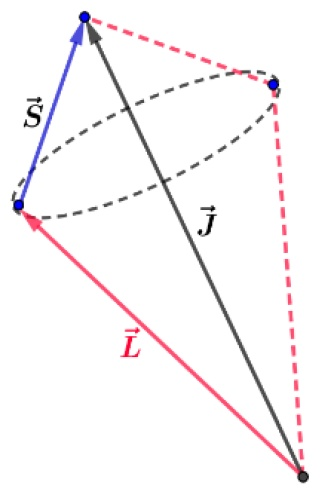
\includegraphics[width=0.4\textwidth]{./Figures/GraficoJLS}
	\caption{Momneto angular total J=L+S}
	\label{fig:GraficoJLS}
\end{figure}



\begin{equation}
	j=\frac{1}{2} ;\quad j=-\frac{1}{2}
\end{equation}	
\end{itemize}

	
Momento angular total de un átomo:
\begin{itemize}
	\item 1. Si:\; $\textcolor{red}{j=l+\frac{1}{2}} \quad\Rightarrow\quad \mid\V{J}\mid =\sqrt{j\big(j+1\big)}\,\hbar = \sqrt{\big(l+\frac{1}{2}\big)\big(l+\frac{3}{2}\big)}\,\hbar$
	\item 2. Si:\; $\textcolor{red}{j=l-\frac{1}{2}} \quad\Rightarrow\quad \mid\V{J}\mid =\sqrt{j\big(j+1\big)}\,\hbar = \sqrt{\big(l+\frac{1}{2}\big)\big(l-\frac{1}{2}\big)}\,\hbar$
\end{itemize}
	
La magnitud del momento angular de espín será:
\begin{equation}
 \mid\overrightarrow{S}\mid =\sqrt{s\big(s+1\big)}\,\hbar = \frac{\sqrt{3}}{2} \quad \text{para} \quad s=\frac{1}{2} 
\end{equation}

De la misma manera se puede obtener los momentos magnético:

%\begin{equation}
\begin{multline}
  \V{\mu}=\V{\mu_{L}}+\V{\mu_{S}}=-\frac{e}{2m}\big(\V{L}+g\,\V{S}\big)=-\frac{e}{2m}\big(\V{L}+2\V{S}\big)=\\
  -\frac{e}{2m}\big(\left[\V{L}+\V{S}\right]+\V{S}\big)= -\frac{e}{2m}\big(\V{J}+\overrightarrow{S}\big)
  \label{eq:uno}
\end{multline}
%\end{equation}

La ecuación (\ref{eq:uno}) nos indica que $\V{\mu}$ no es directamente opuesto a $\V{J}$, salvo que $\V{S} = 0$

Podemos sumar a los vectores $\V{L}$ y $\V{S}$ por que interactúan, si bien mantienen sus orientaciones relativas experimentan una precesión alrededor de $\V{J}$, también precesiona $\V{\mu}$ alrededor de $\V{J}$. La componente de $\V{\mu}$ en la dirección de $\V{j}$ es $\V{\mu_{j}}$. Observemos que hay precesión pese a la ausencia de campo externo al átomo, este fenómeno se llama interacción espín-orbita.

Aquí observamos los gráficos de los dos casos particulares comentados anteriormente, más adelante se ampliara con la interacción $S-L$


\begin{figure}[H]
    \centering
    \includegraphics[width=0.7\textwidth]{./Figures/Gráfico10a}
	\caption{Momento magnético total}
	\label{fig:Grafico10c}
\end{figure}


\begin{figure}[H]
    \centering
    \includegraphics[width=0.7\textwidth]{./Figures/Gráfico10b}
	\caption{Momento magnético total}
	\label{fig:Grafico10c}
\end{figure}


\subsection{Momento magnético total de un átomo}

El momento magnético efectivo del átomo es $\V{\mu_{J}}$, la suma de las componentes $\V{\mu_{L}}$ y $\V{\mu_{S}}$. Si el átomo esta en un campo magnético débil, de tal manera, que no se rompe el acoplamiento entre $\V{L}$ y $\V{S}$ , en este caso $\V{J}$ experimentará una precesión alrededor de $\V{\mu_{H}}$ , el campo exterior.

Esta formulación, que se expone, puede posiblemente ser vista como arbitraria y antojadiza; realmente cobra sentido cuando se ve cómo logra explicar fenómenos experimentales tales como el efecto Zeeman o el experimento de Stern-Gerlach. La realidad es que se crea ad-hoc para explicar estos fenómenos. Nuestro interés es solo comprender el origen del magnetismo

\begin{figure}[H]
    \centering
    \includegraphics[width=0.8\textwidth]{./Figures/Gráfico10c}
	\caption{Momento magnético total}
	\label{fig:Grafico10c}
\end{figure}


\subsubsection{Momento magnético total}

\begin{itemize}
\item Anteriormente se vio que el momento angular orbital y de espín se sumaban formando el momento atómico total. El momento magnético total de un átomo libre tiene tres contribuciones: el momento magnético del núcleo, el momento magnético orbital más el momento magnético del electrón.
\item El núcleo atómico tiene carga y presenta momento magnético, este es $10^3$ veces inferior a los generados por los electrones, luego, no los consideramos en este caso.
\item Luego en un átomo, el campo magnético observado es debido al acoplamiento de estos dos momentos: \textcolor{red}{Orbital} y de \textcolor{red}{Spin}, los cuales generan campos magnéticos y reaccionan ante la presencia de los mismos.
\end{itemize}

Como sabemos el momento angular total $\V{J}$ es la suma del momento del espín $\V{S}$ y el orbital $\V{L}$.

\begin{figure}[H]
    \centering
    \includegraphics[width=0.6\textwidth]{./Figures/Gráfico10d}
	\caption{Momento magnético total átomo libre}
	\label{fig:Grafico10d}
\end{figure}


El momento magnético en la dirección $z$ será:
\begin{equation}
	\mu_{j} = \mu_{zS}+\mu_{zL} = g\,m_{S}\mu_{B}+m_{L}\mu_{B}
\end{equation}

donde las proyecciones se hallan como $\mu_{zS}=\mu_{S}Cos(SJ)$ y $\mu_{zL}+\mu_{L}Cos(LJ)$. Remplazando y operando se llega a:

\begin{equation}
	\mu_{j} = g_{j}\sqrt{j(j+1)}\,\mu_{B} \quad \text{con} \; g_{j}\;  \text{factor de Landé para}\; j    
\end{equation}

\begin{equation}
	g_{j} = 1 + \frac{s(s+1)-l(l+1)+j(j+1)}{2j(j+1)}
\end{equation}

En la figura \ref{fig:Grafico10d} no se tuvieron en cuenta los casos con signos negativos por simplicidad

\subsubsection{Interacción espín-orbita}

\begin{itemize}
	\item La aplicación de un campo magnético externo al átomo produce precesión y divide las líneas espectrales, este fenómeno es llamado efecto Zeeman.
	\item En un átomo los niveles de energía de los electrones son afectados por una interacción interna del átomo, entre el momento magnético del spin y el momento angular orbital. Esta interacción divide las líneas espectrales, en particular en el hidrogeno como se observa en la figura \ref{fig:GraficoInterEspinOrbita}
	\item La interacción spin-orbita es también una interacción con un campo magnético, pero interno, generado por el movimiento orbital del electrón en el propio átomo que llamamos Zeeman interno.
	\item Si se observa las líneas espectrales delhidrogeno con alta resolución, se encuentran que son dobles poco espaciados entre sí. Este fenómeno se llama \textbf{estructura fina}.
	\item Cálculos aproximados demuestran que el campo magnético interno sobre el electrón seria de 0,4 Tesla
	\item Si consideramos el momento dipolar del núcleo, de la interacción de este con el momento orbital y con el spin aparecerán subdivisiones mucho más pequeñas, conocidas como \textbf{estructura hiperfina}.
	
\end{itemize}

\begin{figure}[H]
    \centering
    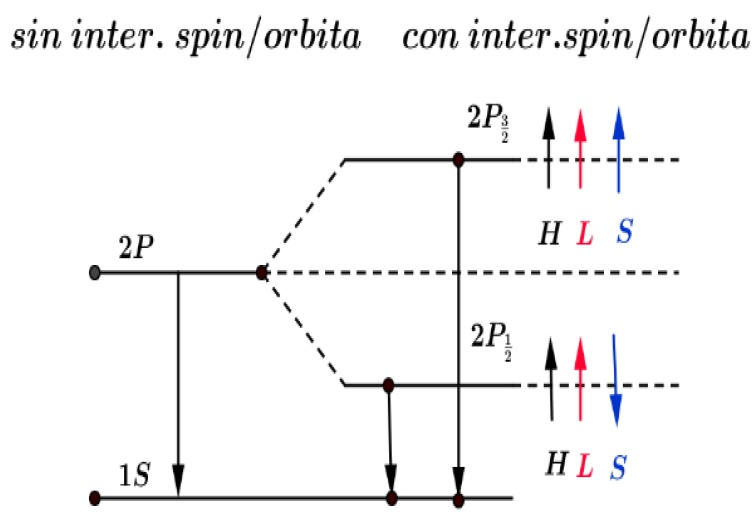
\includegraphics[width=0.6\textwidth]{./Figures/GraficoInterEspinOrbita}
	\caption{Interacción Espín Órbita}
	\label{fig:GraficoInterEspinOrbita}
\end{figure}

La notación $2P\frac{3}{2}$ y $2P\frac{1}{2}$ de la figura \ref{fig:GraficoInterEspinOrbita} es conocida como notación espectroscópica, que no hemos comentado hasta ahora.

\subsection{Átomos con más de un electrón}

El momento angular total de un átomo con más de un electrón es una característica importante por que determina las propiedades magnéticas del átomo.

\textbf{Interacción S-J, Russell-Saunders}
\begin{itemize}
	\item Hay dos formas de sumar los momentos. En los átomos livianos la interacción electrostática es más importante que la magnética, y si los campos magnéticos externos son débiles los espines electrónicos $\V{s_{l}}$ interaccionan entre sí y resultan en un momento angular de espín $\V{S}=\sum_{l}\V{s_{l}}$. Del mismo modo, los momentos angulares orbitales $\V{L_{l}}$ forman el momento angular orbital total $\V{L}=\sum_{l}\V{L_{l}}$. La interacción es llamada de Russell-Saunders, la suma $\V{J}=\sum_{l}(\V{s_{l}}+\V{l_{l}})$ forma el momento angular atómico $\overrightarrow{J}$
\end{itemize}
 
\begin{figure}[H]
    \centering
    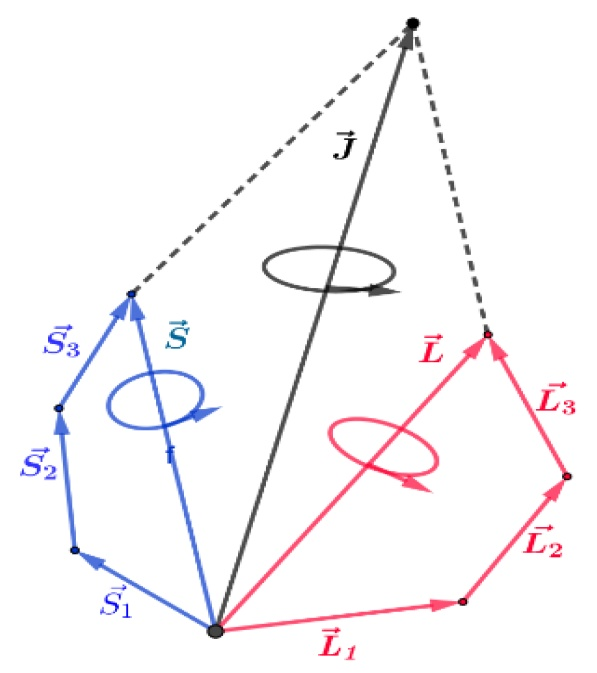
\includegraphics[width=0.6\textwidth]{./Figures/GraficoCaso1}
	\caption{Interacción S-J, Russell-Saunders}
	\label{fig:GraficoCaso1}
\end{figure}

\textbf{Interacción J-J}
\begin{itemize}
	\item Es diferente en los átomos más pesados, donde las interacciones espín-órbita son importantes comparables a las interacciones espín-espín y las órbita-órbita. La interacción $j-j$ es la que prevalece, siendo la opuesta a la Russell-Saunders, y se basa en que la interacción magnética es mucho más importante que la electrostática.
\end{itemize}
 
\begin{figure}[H]
    \centering
    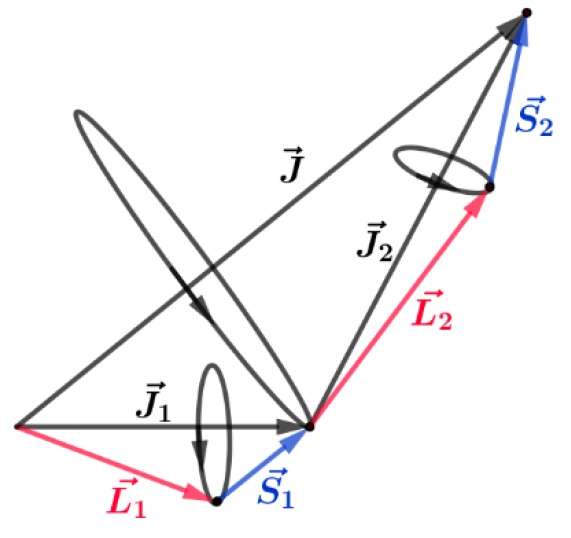
\includegraphics[width=0.6\textwidth]{./Figures/GraficoCaso2}
	\caption{Interacción J-J}
	\label{fig:GraficoCaso2}
\end{figure}

\textbf{Momento orbital bloqueado}
\begin{itemize}
	\item Algo particular sucede en los
elementos de transición. Estos son los que tienen la subcapa $d$ o $f$ parcialmente llena. El término 'elementos de transición' se refiere más comúnmente a los elementos del bloque $d$. El zinc, cadmio y mercurio no cumplen estrictamente con las propiedades de transición. Por lo general son metales de alto punto de fusión. Los elementos de transición del bloque $f$ son conocidos como ''elementos de transición interna''. En los electrones de la serie $3d$ no es posible definir una órbita precisa, debido a las interacciones electrostáticas entre los electrones. Esto estaría indicando una interacción del tipo Russell-Saunders,
\end{itemize}
 
 
\begin{figure}[H]
    \centering
    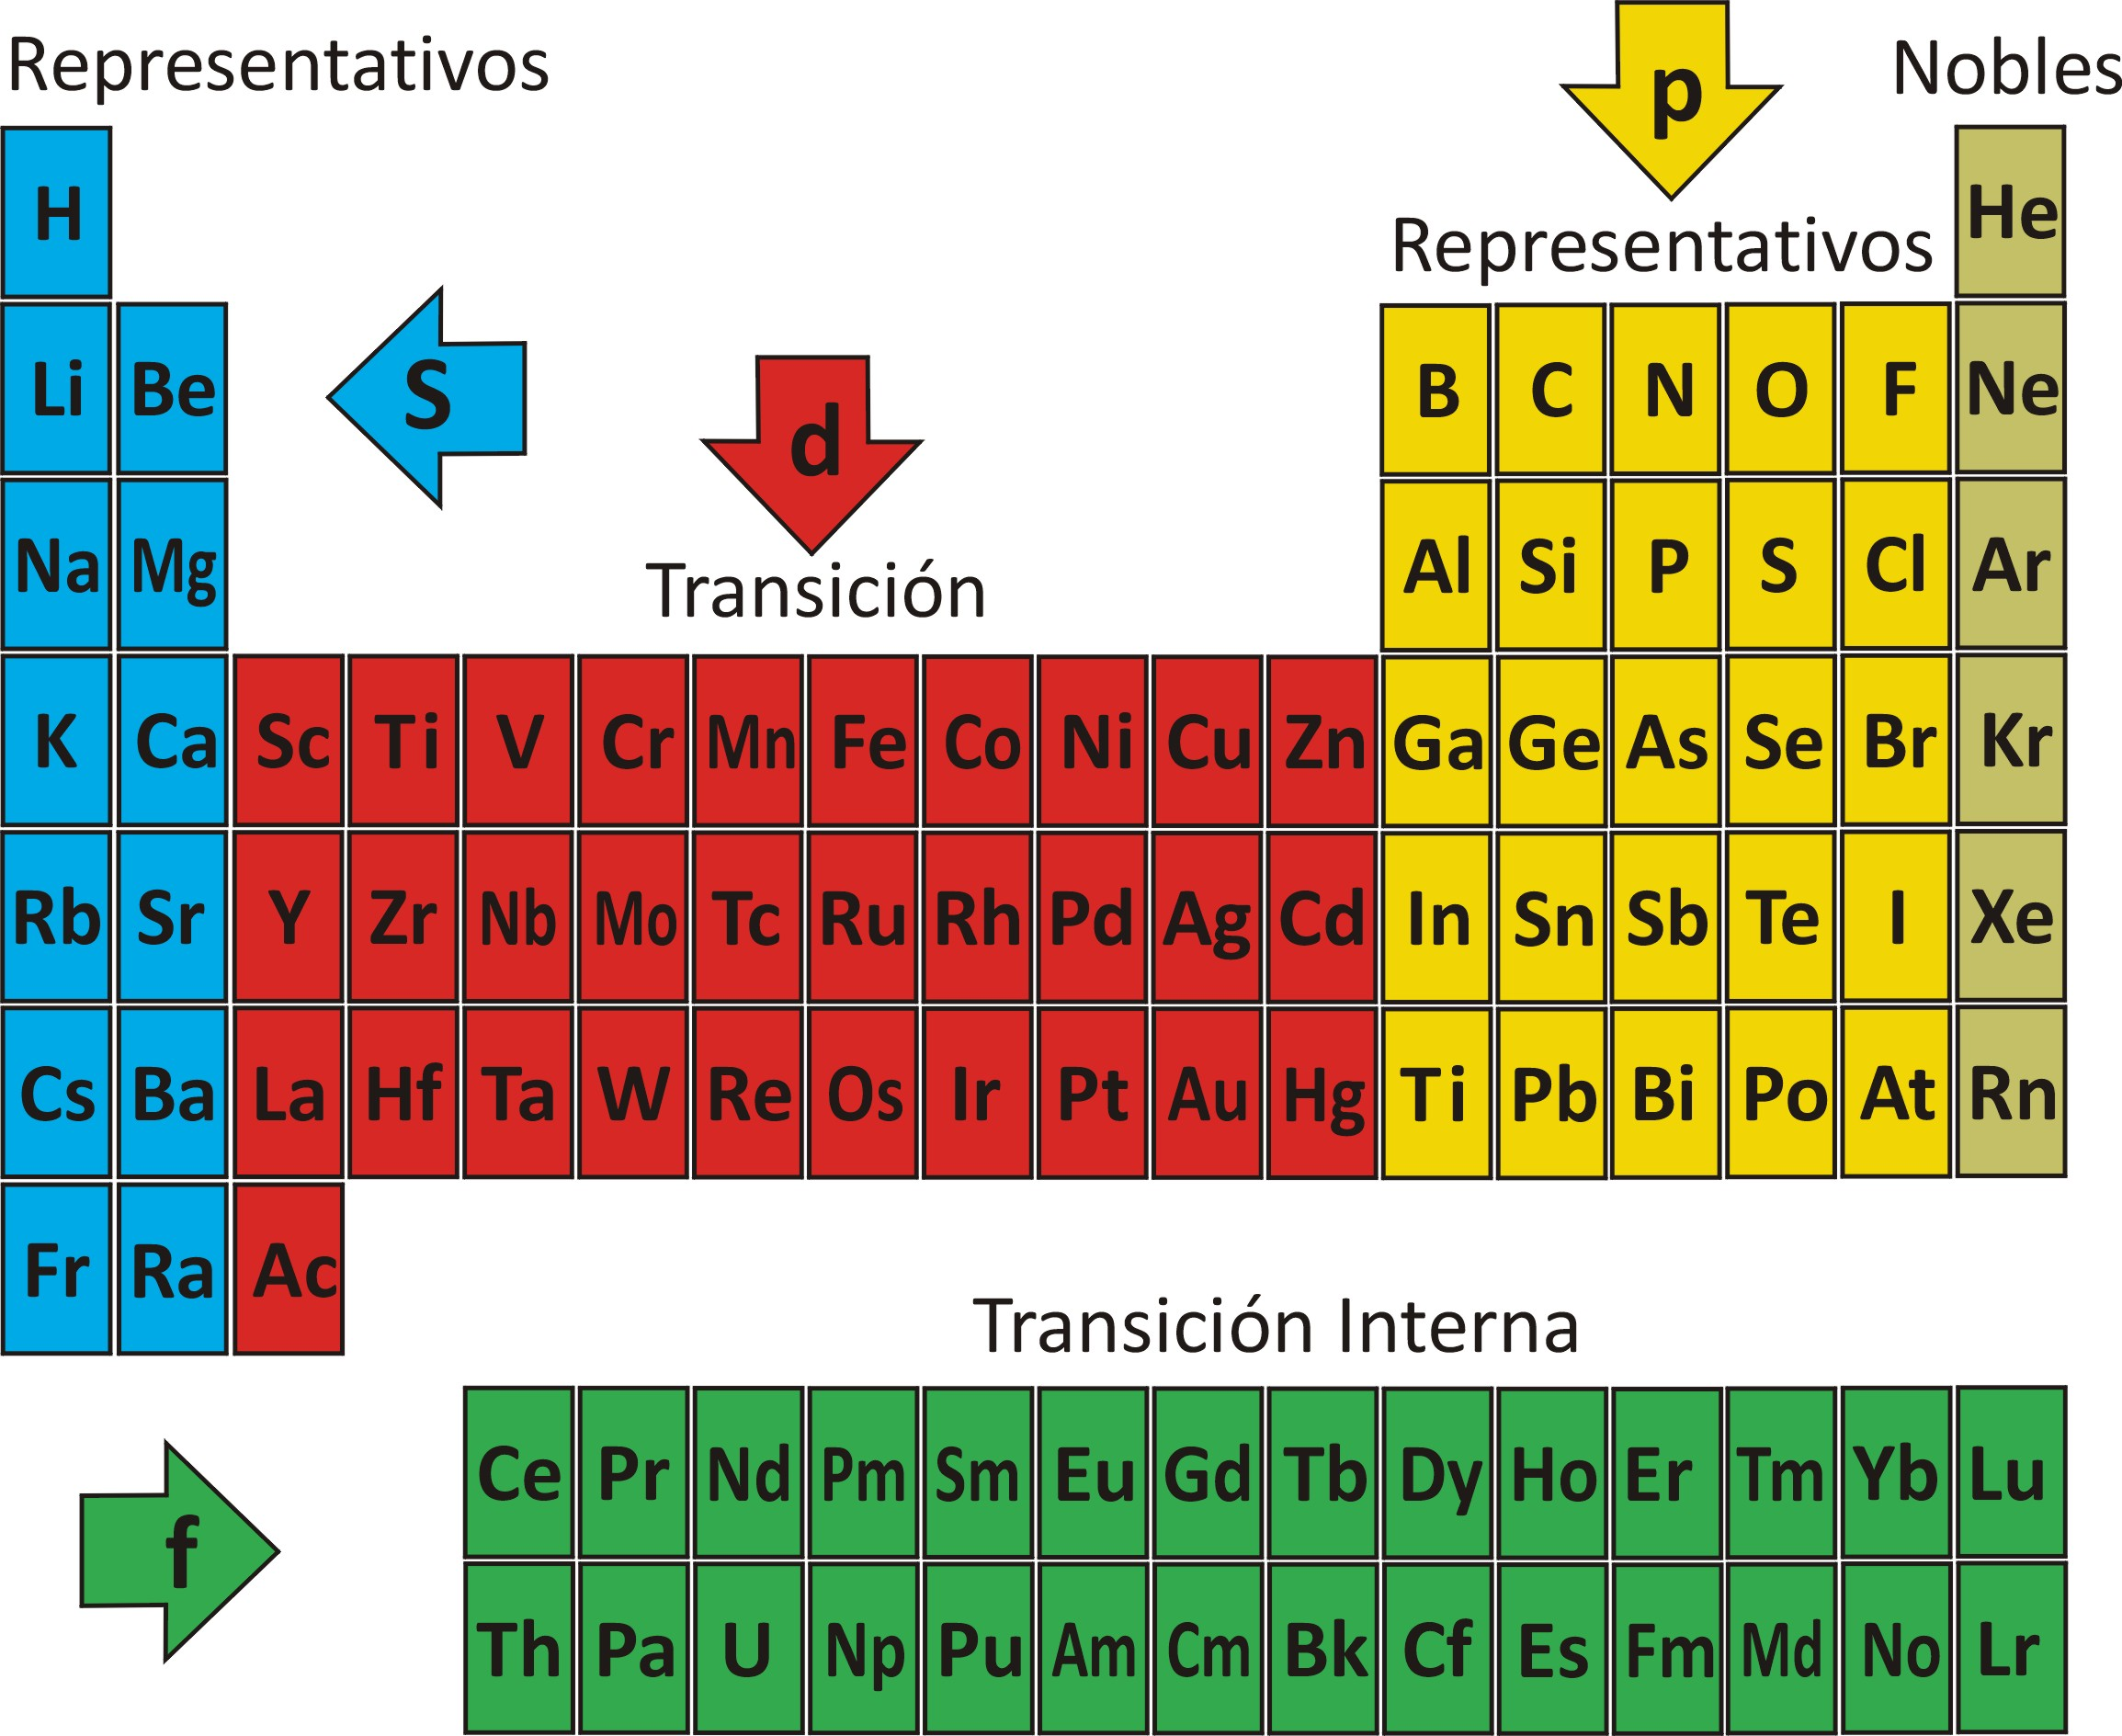
\includegraphics[width=0.8\textwidth]{./Figures/TablaPeriodica}
	\caption{Elementos de transición interna}
	\label{fig:TablaPeriodica}
\end{figure}

luego la suma $\V{J}=\sum_{l}(\V{s_{l}}+\V{l_{l}})$ forma el momento angular atómico $\V{J}$. El momento magnético se calcula $\mu_{j} = g_{j}\sqrt{j(j+1)}\,\mu_B$, sin embargo los resultados experimentales no coinciden con estos
valores y si lo hacen perfectamente con la expresión $g_{s}\sqrt{s(s+1)}\,\mu_B$ como si no existiera el momento orbital. Este fenómeno se expresa diciendo que el momento orbital esta bloqueado y facilita el estudio de los metales que nos interesa.

\textbf{Moraleja: En los metales de transición se considera solo el espín del electrón, (por suerte). Los electrones no apareados les dan las propiedades magnéticas al átomo en el que estén. En tanto en las tierras raras debemos usar el acoplamiento Russell-Sanders.}


Analicemos en particular la configuración electrónica de tres átomos aislados, de
transición de suma importancia en el magnetismo Fe, Ni y Co. Número atómico del Fe= 26, del Ni = 27 y del Co = 28
\vspace{1.0cm}

\begin{figure}[H]
    \centering
    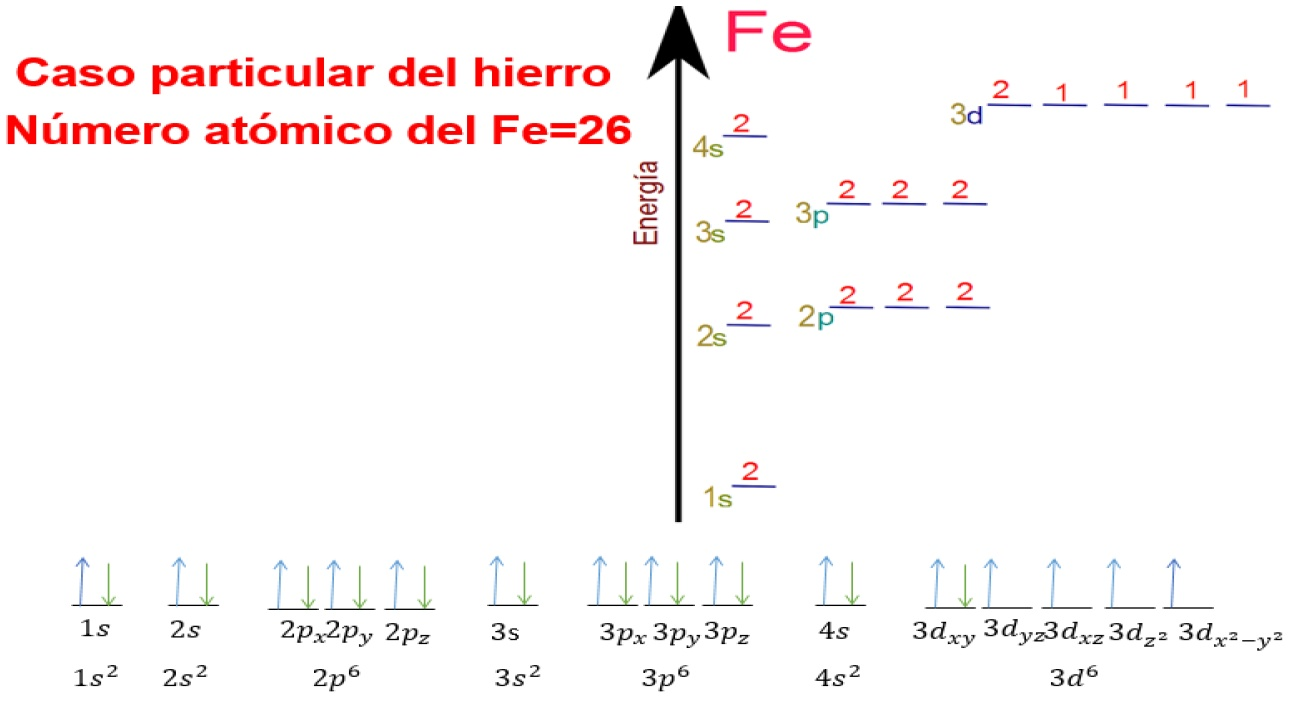
\includegraphics[width=1.0\textwidth]{./Figures/casoDelFe}
	\caption{Distribución electrónica del Hierro}
	\label{fig:casoDelFe}
\end{figure}

\begin{figure}[H]
    \centering
    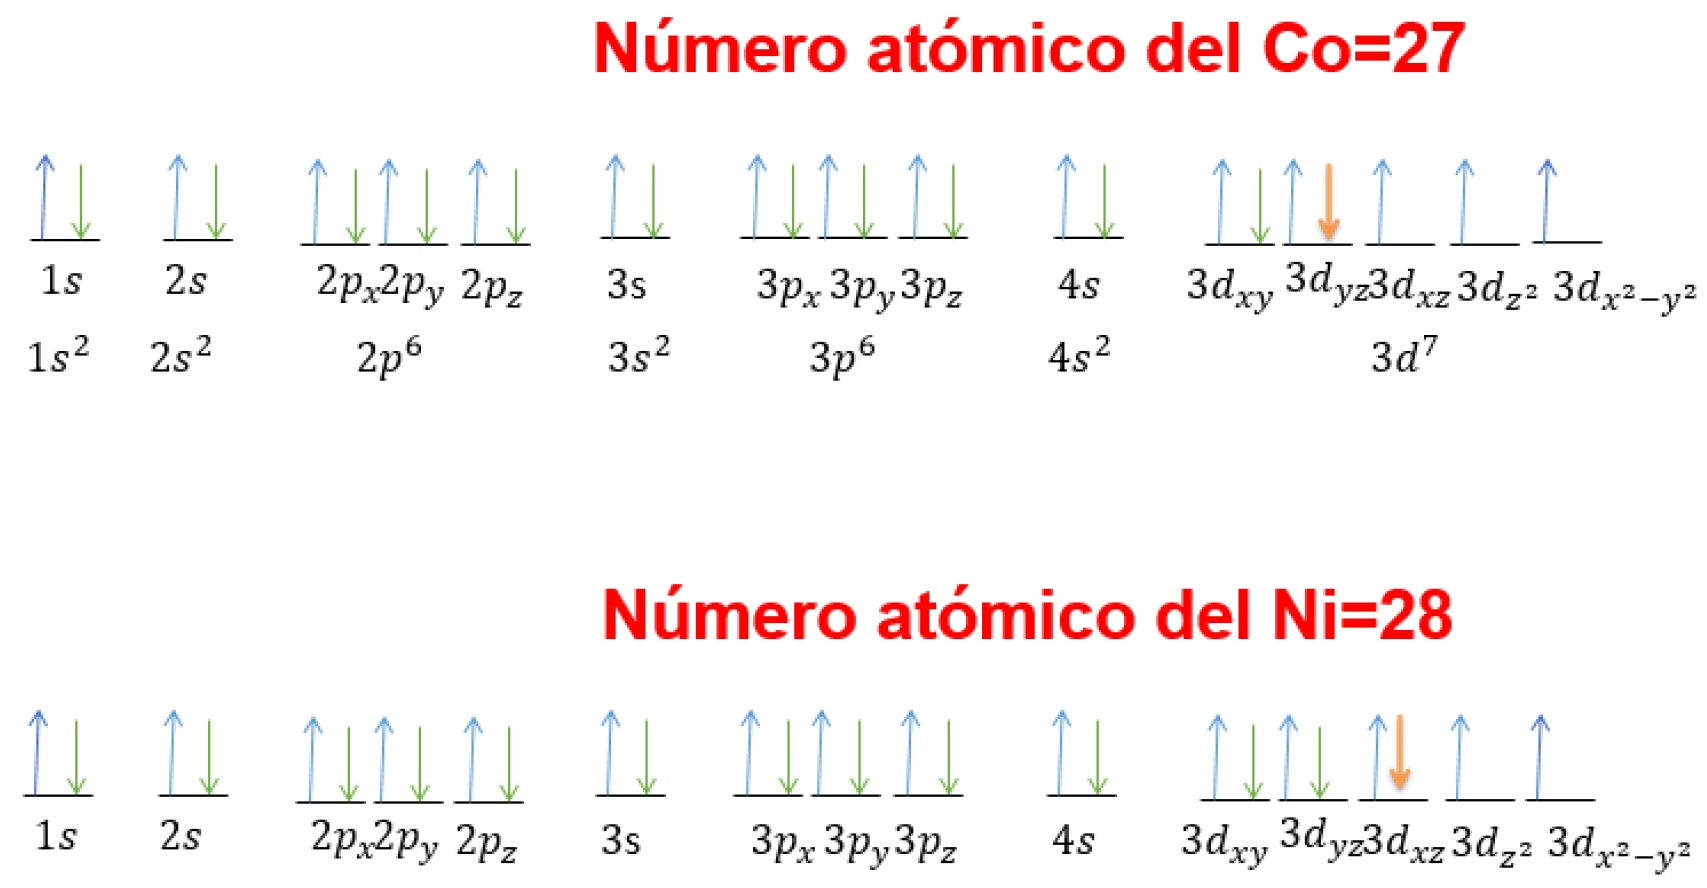
\includegraphics[width=1.0\textwidth]{./Figures/casoDelNiCo}
	\caption{Distribución electrónica del Níquel y el Cobalto}
	\label{fig:casoDelNiCo}
\end{figure}

En la figura \ref{fig:momMagElemTransicion4} vemos la distribución de electrones correspondiente al Fe en distintos estados de oxidación.

\begin{figure}[H]
    \centering
    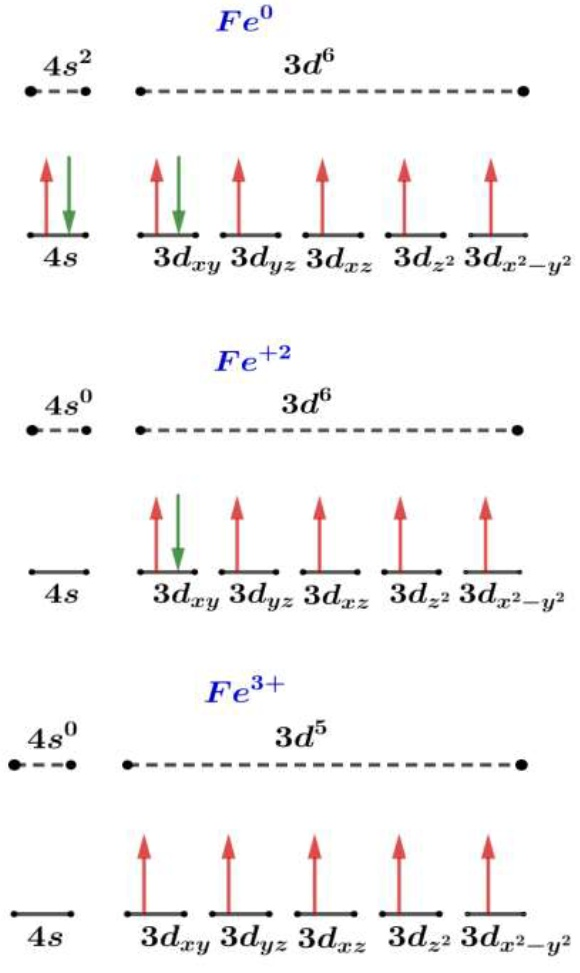
\includegraphics[width=0.6\textwidth]{./Figures/momMagElemTransicion4}
	\caption{Fe en distintos estado de oxidación}
	\label{fig:momMagElemTransicion4}
\end{figure}


\begin{itemize}
	\item Vemos que los átomos con capas externas completas tienen momento magnético cero, (gases inertes pero también Zn, Cd, Hg ), los elementos con solo electrones en la capa $s$ no tienen momento orbital ($l=0$), en estos casos el momento magnético atómico se debe solo al espín. Los alcalinos con un solo electrón en la capa $s$ tienen un momento magnético de un magnetón, lo mismo es cierto para el (Cu, Ag, Au).
	\item Aquellos que tienen una capa interna no completa poseen un momento magnético importante (elementos de transición), estos son los casos que nos interesa. Como ya mencionamos los elementos de transición tienen el momento orbital bloqueado.
\end{itemize}

\subsection{Ejemplos de los grupos 3d y 4f}

Tenemos la estructura $3d^{n} 4s^{2}$ el momento magnético es predominantemente debido al espín, hay poco blindaje de los electrones en el nivel $4s, L\approx0$.


\begin{figure}[H]
    \centering
    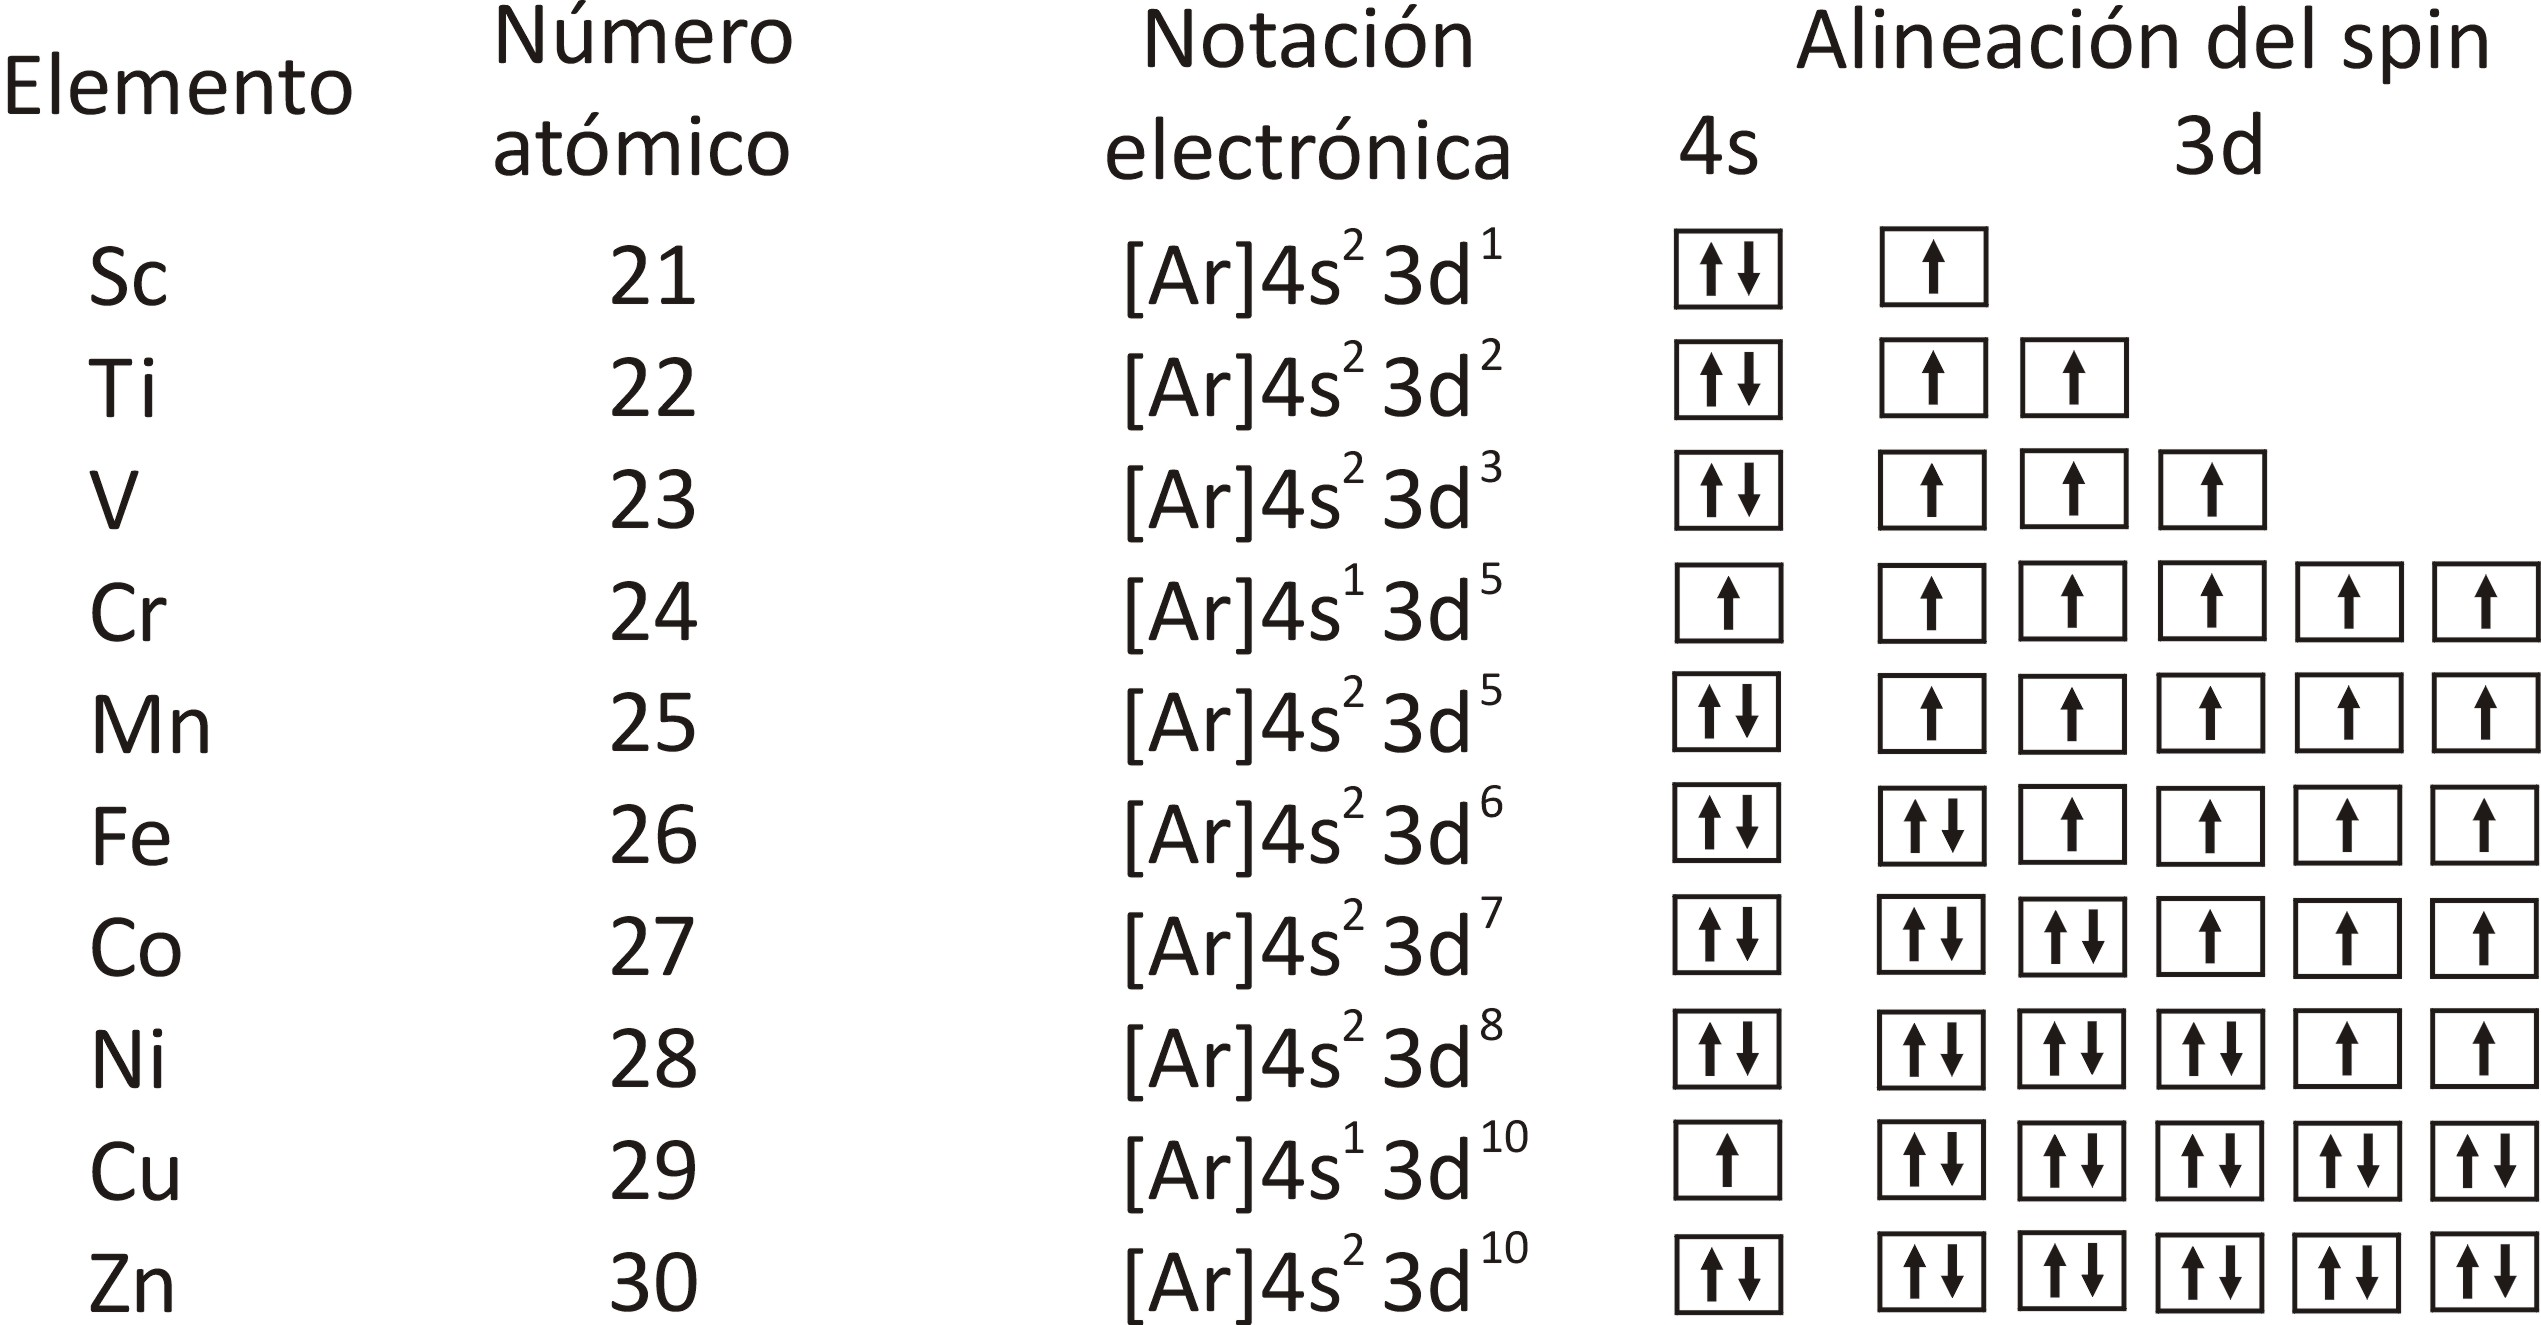
\includegraphics[width=1.0\textwidth]{./Figures/AlineacionDelEspin2}
	\caption{Alineacion del espín grupos 4s 3d}
	\label{fig:AlineacionDelEspin2}
\end{figure}

Tenemos la estructura $4f^{n} 5s^{2} 5p^{6} 6s^{2}$ el momento magnético es predominantemente debido a $L+S$, hay
fuerte blindage de los electrones en los niveles completos $6s\; y\; 5p$. El momento magnético es mayor que el
del grupo $3d$.

\begin{figure}[H]
    \centering
    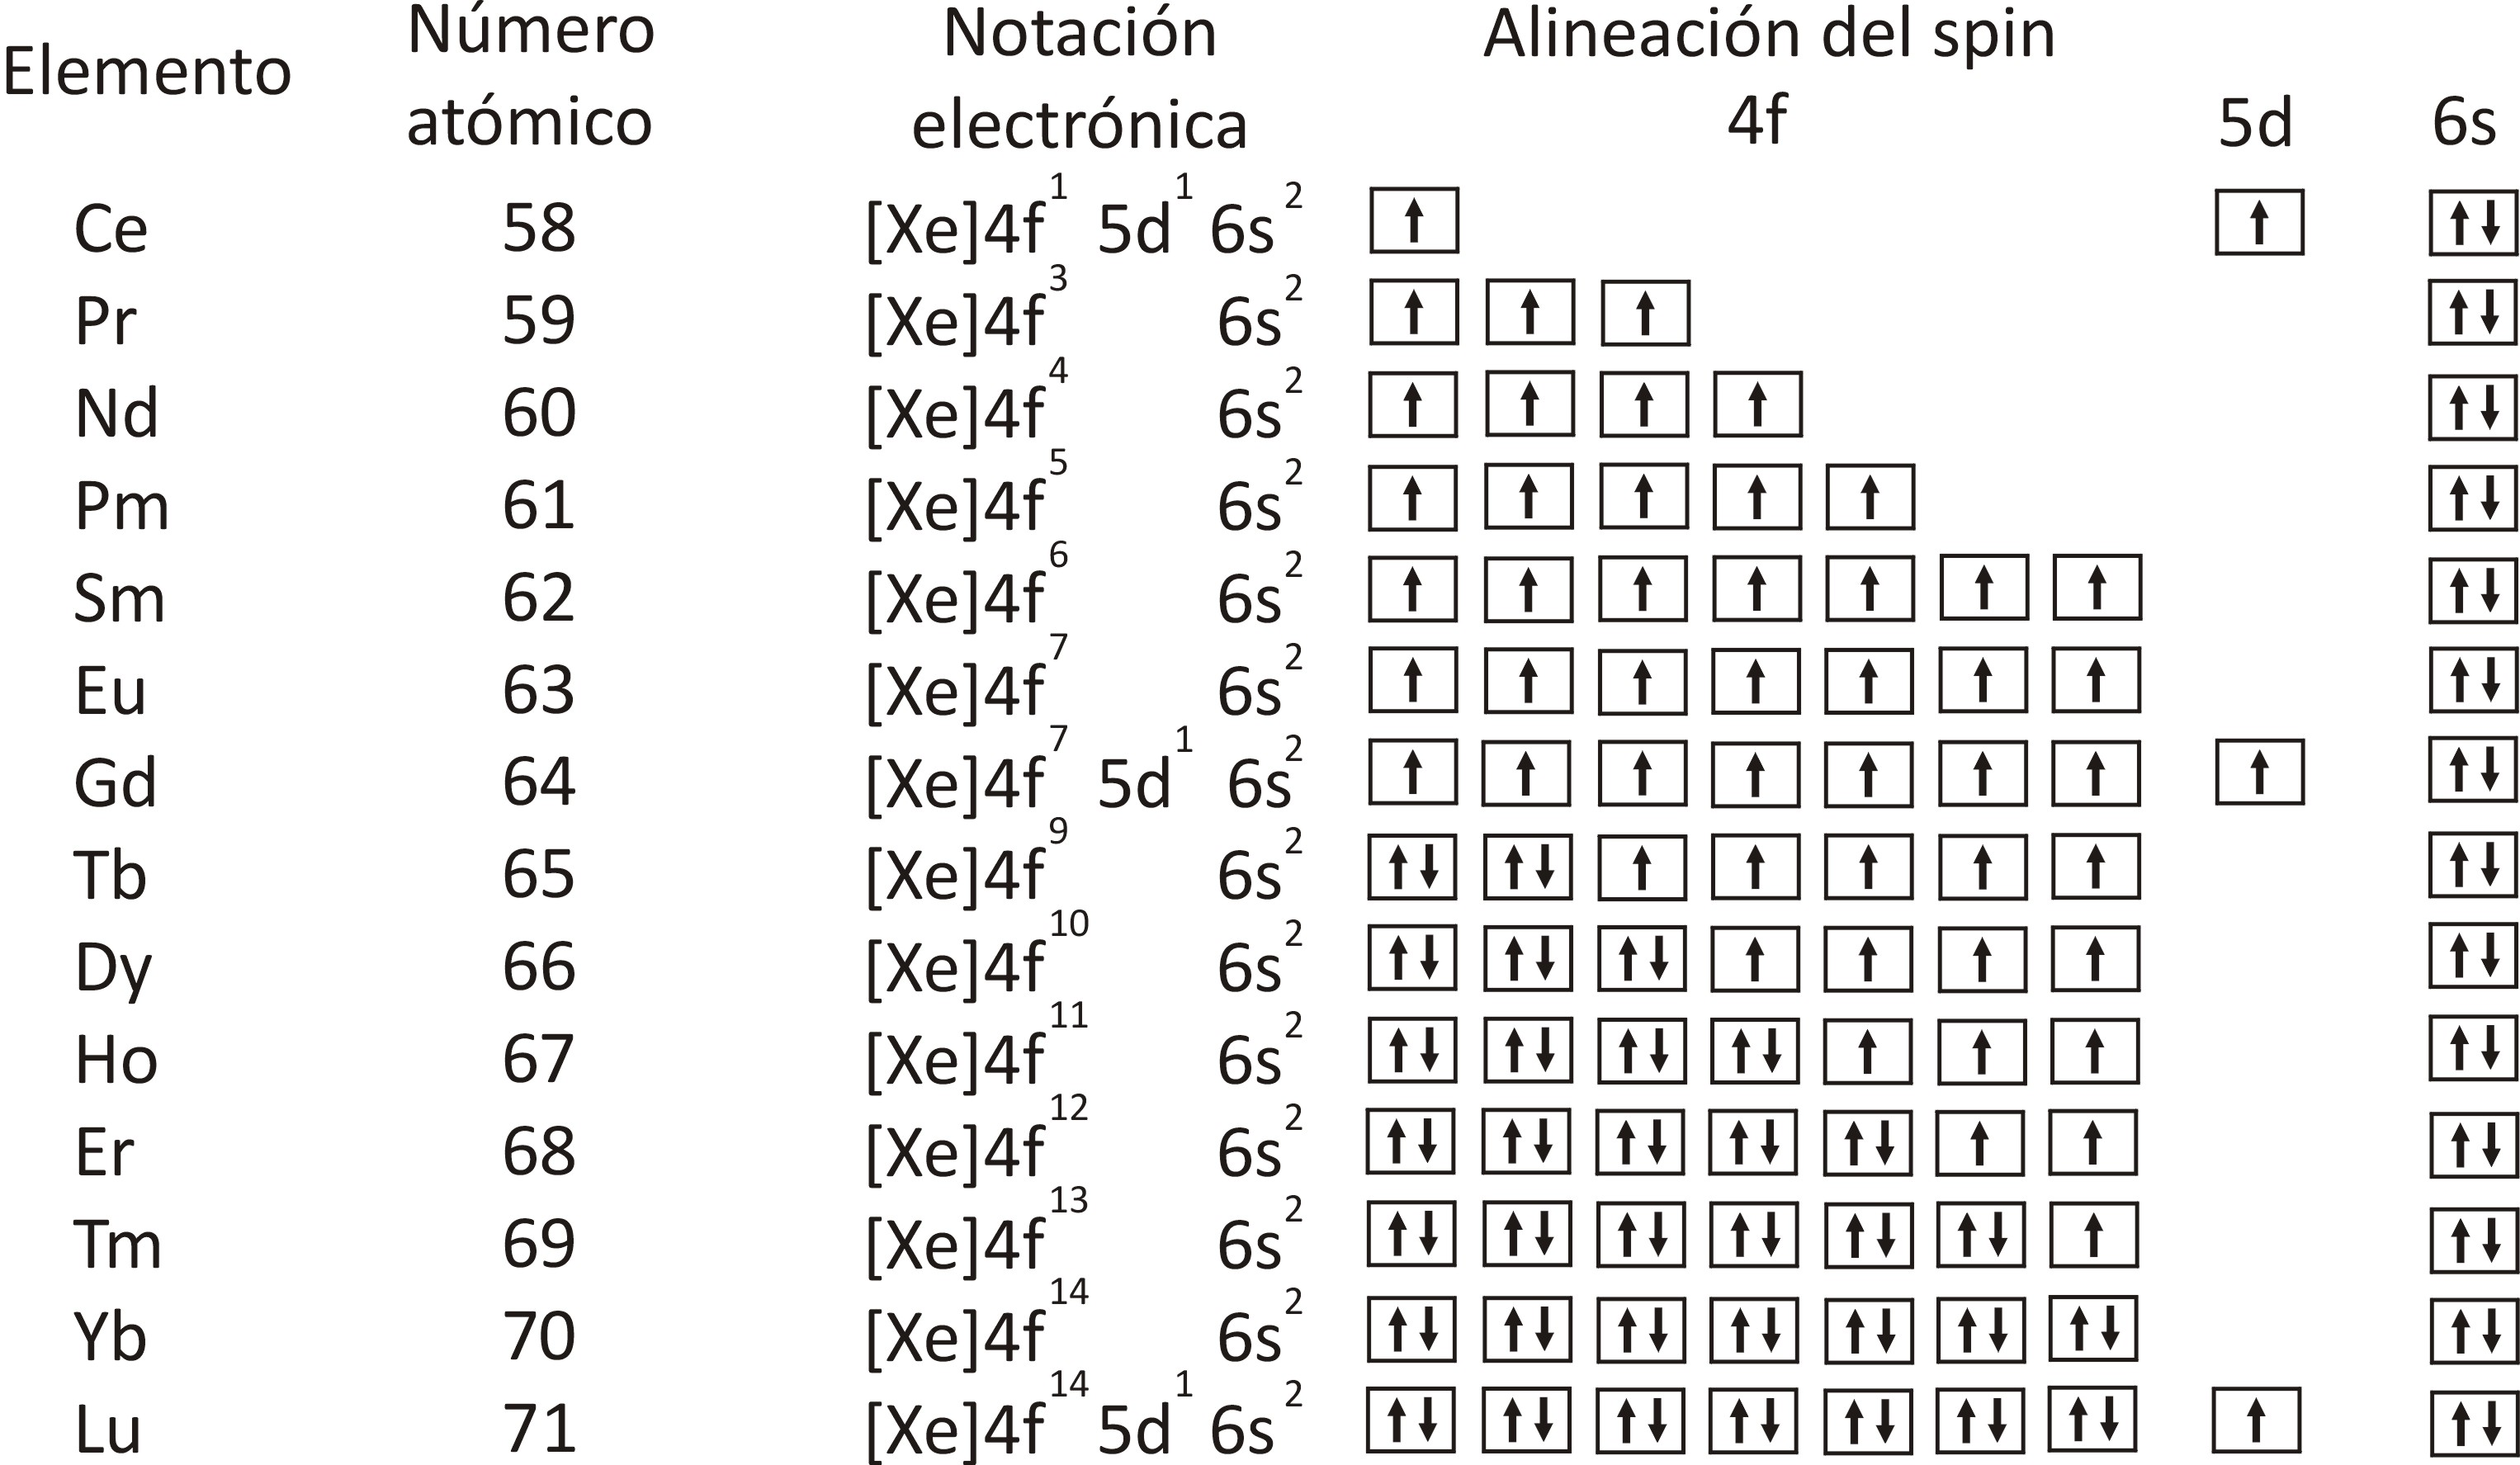
\includegraphics[width=1.0\textwidth]{./Figures/AlineacionDelEspin3grupo4f}
	\caption{Alineacion del espín grupo 4f}
	\label{fig:AlineacionDelEspin3grupo4f}
\end{figure}

Como se comento previamente los elementos de transición tienen el momento orbital bloqueado lo cual permite simplificar el cálculo del momento magnético atómico, pues solo debemos tener en cuenta el número de electrones no apareados.

\begin{equation}
	\mu_{j} = g_{j}\sqrt{j(j+1)}\,\mu_{B} \quad \text{luego} \quad \mu_{j}=2\sqrt{s(s+1)}\,\mu_{B}
\end{equation}

veamos el momento magnético de los iones de los elementos $3d$ en función del número $n$ de electrones
desapareados en unidades de $\mu_{B}$ magnetones de Bohr

\begin{equation}
	\mu_{j} = \sqrt{n(n+1)}\,\mu_{B} 
\end{equation}

\begin{figure}[H]
    \centering
    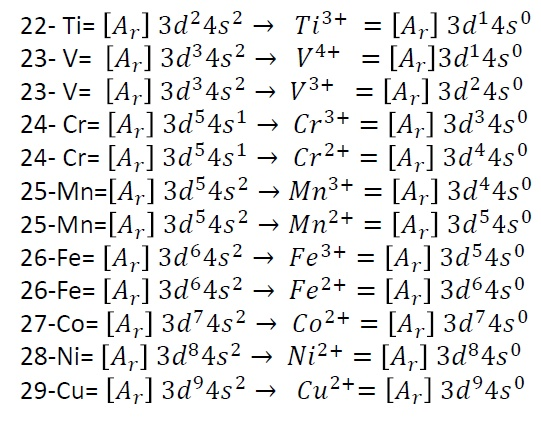
\includegraphics[width=0.8\textwidth]{./Figures/momMagElemTransicion3}
	\caption{Elementos de transición con momento orbital bloqueado}
	\label{fig:momMagElemTransicion3}
\end{figure}

\subsubsection{Momento magnético de los Elementos de transición interna}

\begin{figure}[H]
    \centering
    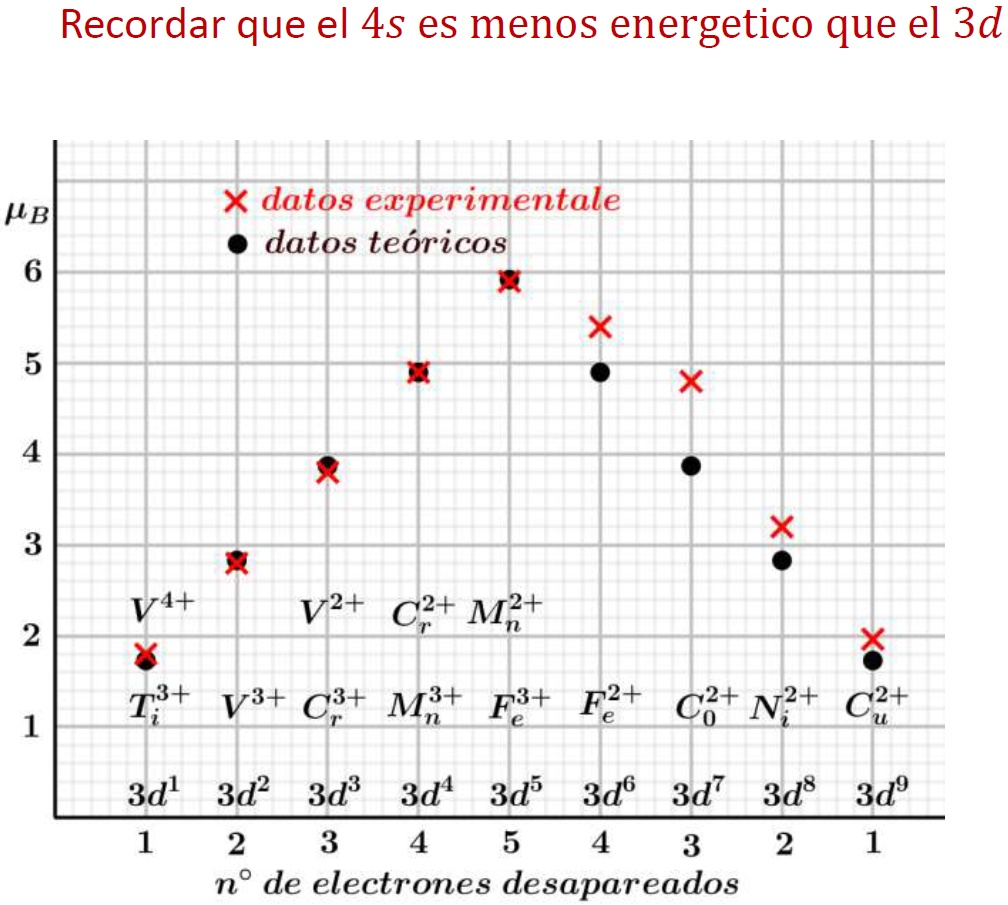
\includegraphics[width=1.0\textwidth]{./Figures/momMagElemTransicion2a}
	\caption{Momento magnético de los Elementos de transición interna}
	\label{fig:momMagElemTransicion2}
\end{figure}

\textbf{Tabla Periódica de los elementos que tienen electrones no apareados}

Los electrones no apareados les dan propiedades magnéticas al elemento en el que están y generalmente alteran sus propiedades ópticas

\begin{figure}[H]
    \centering
    \includegraphics[width=1.0\textwidth]{./Figures/TablaPeriodica2}
	\caption{Elementos de electrones desapareados}
	\label{fig:TablaPeriodica2}
\end{figure}




\section{Magnetismo de moléculas y compuestos químicos}

Hasta ahora conocemos tanto el origen del diamagnetismo como el del paramagnetismo. Podemos decir que átomos o iones podrían ser diamagnéticos o paramagnéticos. Vimos también un ejemplo de elementos paramagnéticos que dejan de serlo cuando se unen químicamente. Nos queda por estudiar el caso de moléculas y compuestos químicos. Si bien el caso del magnetismo de las moléculas o de compuestos es complejo podemos avanzar un poco más, pues nos servirá como introducción al ferromagnetismo.

\subsection{Teoría de los Orbitales Moleculares (TOM)}

La TOM es una metodología de mucha utilidad para determinar las propiedades magnéticas de moléculas y la estabilidad de las mismas. Sabemos que los átomos poseen orbitales donde la probabilidad de hallar electrones es máxima. La TOM supone también, que las moléculas poseen orbitales moleculares en donde se encuentran los electrones. Se asume que los electrones se mueven bajo la influencia de todos los núcleos que componen la molécula. Los orbitales moleculares se hallan como combinación lineal de los orbitales atómicos.

Si suponemos que la función de onda del orbital molecular es $\Psi$ y $\chi$ es la función de onda de los orbitales atómicos entonces:

\begin{equation}
	\Psi_{j} = \sum_{i=1}^{n}C_{ij}\chi_{i}
\end{equation}

Durante la formación de la molécula, él o los átomos y sus orbitales se acercan y comienzan a interactuar, formando los nuevos orbitales moleculares que pertenecen a la molécula en su totalidad y no a un solo átomo.

\subsection{Magnetismo de moléculas y compuestos químicos}

\begin{itemize}
	\item El numero de orbitales de orbitales moleculares es igual al número de orbitales atómico que se solapan. 		
	\item Para ir avanzando sobre el tema tomemos el ejemplo de una molécula formada por átomos iguales $H_{2}$ . En el esquema se observa los dos orbitales atómicos $1s$, que al interactuar formas los orbitales moleculares enlazante $\sigma_{1s}$ de menor energía que el antideslizante $\sigma_{1s}^{*}$ . Por supuesto, los niveles energéticos de los átomos de hidrógeno, antes de la reacción son iguales.
	
\begin{figure}[H]
    \centering
    \includegraphics[width=0.6\textwidth]{./Figures/MagMolecular}
	\caption{Magnetismo Molecular}
	\label{fig:MagMolecular}
\end{figure}

Se llama orden de enlace ($OE$) al parámetro que indica la estabilidad de la unión. Se define como la mitad de la diferencia entre el número de electrones en los Orbitales enlazantes menos el número de electrones en los orbitales antienlazantes. Si el resultado es positivo la unión es estable

\begin{equation}
	OE=\frac{OE-OA}{2}=\frac{2-0}{2}=1
\end{equation}
	
	
	\item Si a la molécula $h_{2}$ la irradiamos con luz ultravioleta puede pasar un electrón al orbital antienlazante, absorbiendo energía con lo cual el $OE$ seria 0, luego la molécula deja de existir.
	
	\item Estudiemos el caso de una molécula de gas noble que no existe $hE_{2}$ en este caso será:

En todos los casos se debe respetar el \textbf{Principio de Pauli}: recordemos que no puede haber dos electrones con todos sus números cuánticos iguales, en el mismo estado dentro del mismo sistema. y el \textbf{Principio de Hund} que dice: Los electrones se ubican dentro de los orbitales de la misma energía de manera que estén desapareados al máximo

\begin{figure}[H]
    \centering
    \includegraphics[width=0.6\textwidth]{./Figures/MagMolecularHe2}
	\caption{Magnetismo Molecular del $He_{2}$}
	\label{fig:MagMolecular}
\end{figure}

\begin{equation}
	OE=\frac{OE-OA}{2}=\frac{2-2}{2}=0
\end{equation}

Luego, la molécula no es estable.
\end{itemize}


\subsubsection{Casos en que entra en juego el segundo nivel energético}

En el caso que interactúen orbitales $2s$ el procedimiento es igual al caso anterior. En la figura, de abajo, se observa un esquema de los orbitales $s$, con n significamos el número cuántico principal, puesto que todos los $s$ serán Iguales.

\begin{figure}[H]
    \centering
    \includegraphics[width=0.6\textwidth]{./Figures/SegundoNivelEnergetico}
	\caption{Segundo nivel energético orbitales $s$}
	\label{fig:SegundoNivelEnergetico}
\end{figure}

Difiere un poco cuando trabajos con los orbitales $2p$, ya que, no son esféricos y se sitúan a lo largo de los tres ejes $x$, $y$, $z$ del espacio. Para entender un poco mejor como se unen los átomos seguiremos trabajando con los orbitales. A medida que los átomos se acercan comienzan a interactuar los orbitales atómicos y forman, por combinación lineal los orbitales moleculares. Se dan distintas posibilidades según que orbitales atómicos se enfrentan. Supongamos que enfrentamos dos órbita $2p_{x}$, como indica el esquema, esta interacción dará origen a dos orbitales moleculares.

\begin{figure}[H]
    \centering
    \includegraphics[width=0.7\textwidth]{./Figures/Molecula2doNivel1}
	\caption{Segundo nivel energético dos orbitales $s$}
	\label{fig:Molecula2doNivel1}
\end{figure}

En la figura \ref{fig:Molecula2doNivel2} se observa un esquema donde reaccionan dos orbitales atómicos enfrentado en la dirección $x$ mientras que en la figura \ref{fig:Molecula2doNivel3} los orbitales que reaccionan están en la dirección $y$.

\begin{figure}[H]
    \centering
    \includegraphics[width=0.7\textwidth]{./Figures/Molecula2doNivel2}
	\caption{Orbitales enfrentados en la dirección $x$}
	\label{fig:Molecula2doNivel2}
\end{figure}

\begin{figure}[H]
    \centering
    \includegraphics[width=0.7\textwidth]{./Figures/Molecula2doNivel3}
	\caption{Orbitales enfrentados e la dirección $y$}
	\label{fig:Molecula2doNivel3}
\end{figure}
	
	
Algo similar sucede si los orbitales paralelos estuviesen en la dirección Z. En estos dos últimos casos los orbitales moleculares se designan con $\pi_{np_{y}}$ , $\pi_{np_{z}}$ o $\pi_{np_{y}}^{*}$ , $\pi_{np_{z}}^{*}$

\subsubsection{Ejemplo: molécula del $Ni_{2}$}

\begin{itemize}
	\item Comenzamos por la configuración electrónica del Nitrógeno ($Z=7$):
	\begin{equation}
		1s^{2}2s^{2}2p^{1}_{x}2p^{1}_{y}2p^{1}_{z}
	\end{equation}
	\item Los orbitales se llenan de acuerdo a las principios de \textbf{Pauli y Hund}. 
	\item Los orbitales atómicos tienen las mismas energía, por eso se encuentran al mismo nivel. No pasaría lo mismo si los átomos son distintos.
	\item Los orbitales moleculares de menor enegía se llenan primero.
	\item En este caso los orbitales enfrentados son los $2p_{z}$
	\item \textbf{Esta molécula es diamagnética, puesto que tiene los electrones apareados, los átomos son paramagnéticos}
	\item Si los átomo que reaccionan tiene pocos electrones, no solo hay interacción $s-s$ y $p-p$ sino que aparece otra interacción $s-p$ que modifica los niveles de los orbitales moleculares esto se observa en el esquema de la figura \ref{fig:EjemploNi2}.
\end{itemize}

\begin{figure}[H]
    \centering
    \includegraphics[width=0.6\textwidth]{./Figures/EjemploNi2}
	\caption{Molécula de $Ni_{2}$}
	\label{fig:EjemploNi2}
\end{figure}

\newpage

\subsubsection{Interacción cruzada}

\textbf{Para átomos con $N \leq 7 $ electrones}

\begin{figure}[H]
    \centering
    \includegraphics[width=0.7\textwidth]{./Figures/interaccionCruzada7a}
	\caption{Interacción cruzada $N \leq 7$}
	\label{fig:interaccionCruzada7a}
\end{figure}


\textbf{Para átomos con $N>7$ electrones}

\begin{figure}[H]
    \centering
    \includegraphics[width=0.7\textwidth]{./Figures/interaccionCruzada7b}
	\caption{Interacción cruzada $N > 7$}
	\label{fig:interaccionCruzada7b}
\end{figure}


\newpage
\subsubsection{Caso del Oxígeno $Z=8$}


\textbf{$O_{2}$ - Paramagnético:}

\begin{figure}[H]
    \centering
    \includegraphics[width=0.7\textwidth]{./Figures/interaccionCruzadaOxigenoA}
	\caption{$O_{2}$ Paramagnético}
	\label{fig:interaccionCruzadaOxigenoA}
\end{figure}

\textbf{$O_{2}^{+}$ - Paramagnético:}

\begin{figure}[H]
    \centering
    \includegraphics[width=0.7\textwidth]{./Figures/interaccionCruzadaOxigenoC}
	\caption{$O_{2}^{+}$ Paramagnético}
	\label{fig:interaccionCruzadaOxigenoC}
\end{figure}


\textbf{$O_{2}^{2+}$ - Diamagnético:}

\begin{figure}[H]
    \centering
    \includegraphics[width=0.7\textwidth]{./Figures/interaccionCruzadaOxigenoB}
	\caption{$O_{2}^{2+}$ Diamagnético}
	\label{fig:interaccionCruzadaOxigenoB}
\end{figure}


\textbf{$O_{2}^{2-}$ - Diamagnético:}

\begin{figure}[H]
    \centering
    \includegraphics[width=0.6\textwidth]{./Figures/interaccionCruzadaOxigenoD}
	\caption{$O_{2}^{2-}$ Diamagnético}
	\label{fig:interaccionCruzadaOxigenoD}
\end{figure}

\subsubsection{Compuestos de átomos distintos}

Hasta ahora hemos visto moléculas di atómicas de átomos iguales, nos está faltando el magnetismo de moléculas formadas por átomos distintos. En este caso la dificultad está en que al no ser átomos iguales, estos no tienen los mismos niveles de energía. Tengamos presente que los átomos más electronegativos tienen menor energía.

Los orbitales moleculares se llenan como hasta ahora teniendo en cuenta los principios de Pauli y Hund.

Veamos dos casos clásicos $CO$ y $NO$.

\textbf{Para el CO:}

Se debe comenzar con la configuración electrónica de cada elemento
\begin{equation}
\begin{aligned}
	C: He+ 2s^{2}2p^{2} \\
	O: He+ 2s^{2}2p^{4}
\end{aligned}
\end{equation}

No se dibujan los niveles $1s^{2}$ por ser iguales en todos los casos.
Los niveles moleculares se observan en la figura \ref{fig:CO2Diamagnetico}:

\begin{figure}[H]
    \centering
    \includegraphics[width=0.6\textwidth]{./Figures/CO2Diamagnetico}
	\caption{$CO_{2}$ Diamagnético}
	\label{fig:CO2Diamagnetico}
\end{figure}


\textbf{Para el NO:}

La configuración electrónica del nitrógeno es
\begin{equation}
	N: He+ 2s^{2}3p^{3}
\end{equation}
No dibujamos el vector que Indica la dirección en la que aumenta la energía pues es similar al caso anterior.
Por tener un electrón desapareado esta molécula es paramagnética.

\begin{figure}[H]
    \centering
    \includegraphics[width=0.6\textwidth]{./Figures/CO2Paramagnetico}
	\caption{$CO_{2}$ Paramagnético}
	\label{fig:CO2Paramagnetico}
\end{figure}

Tengamos presente que:

\begin{itemize}
	\item Todas las moléculas formadas por átomos distintos presentan esquemas de energía similares.
	\item Estamos comentando solo los casos más simples, existen moléculas donde la complicación es mayor.
	\item En todos estos casos se podría haber calculado el orden de enlace,
\end{itemize}










\chapter{Susceptibilidad magnética} % Main chapter title



\begin{center}

. . . . .Todo lo que usted quiera, concluyó un convidado, \\
pero si no cree en el magnetismo después de eso, \\
¡es usted un ingrato, mi querido señor!


\hspace{5.6cm} Magnetismo\\
\hspace{4.6cm} Guy
de maupassant  
\end{center}


\vspace{0.5cm} 

\section{susceptibilidad magnética} 
El campo magnético dentro de una sustancia se lo llama inducción magnética $\V{B}$ y difiere del campo magnético en el vacío $\V{H}$. La diferencia es el aporte del medio material llamado magnetización $\V{M}_{0}$ momento dipolar inducido por unidad de volumen

\begin{equation*}
\V{B}= \V{H} + 4\pi\V{M}\; \text{CGS} \qquad  \V{B}= \mu_{0}(\V{H} +\V{M})\; \text{SI}
\end{equation*}

Donde $\mu_{0}$ es la permeabilidad magnética del vacío. La relación entre $\V{M} \left[ \dfrac{a}{m} \right]$ Y $\V{h} \left[ \dfrac{a}{m} \right]$ se llama susceptibilidad magnética por unidad de volumen $\chi_{V}$ y es adimensional:

\begin{equation*}
\chi_{V} = \dfrac{\vert\V{M}\vert}{\vert\V{H}\vert}
\end{equation*}

También se puede escribir $\V{B}= \mu_{0}(\V{H} + \V{M}) = \mu_{0}(\V{H} + \chi_{v}\V{H}) = \mu_{0}(1 + \chi_{v})\V{H} = \mu \V{H}$ donde $\mu$ es la permeabilidad magnética.

La susceptibilidad $\chi_{v}$ es análoga a la $\chi_{e}$ llamada susceptibilidad eléctrica y en ambos casos miden la respuesta del medio al campo magnético externo o al campo eléctrico externo También es usada la susceptibilidad magnética molar $\chi=V_{m}\chi_{v}$ donde $V_{m}$ es el volumen molar. Si la magnetización de la muestra aumenta, la susceptibilidad magnética es positiva y si disminuye es negativa. La susceptibilidad magnética se medida por la balanza de Gouy\footnote{La balanza de Gouy, inventada por el físico francés Louis Georges Gouy (1854-1926), mide la susceptibilidad magnética de una muestra, a través de su atracción o repulsión por un gradiente de campo magnético. La muestra se introduce en un recipiente cilíndrico alargado, suspendido de una balanza y penetrando parcialmente entre los polos de un imán. La balanza mide el cambio de masa aparente al ser repelida o atraída por la región de alto campo magnético entre los polos. Este método es de importancia histórica, de interés didáctico y permite determinaciones susceptométricas a un coste muy bajo. En la actualidad es común el uso de métodos mucho más sensibles como los magnetómetros dotados de SQUID}.

La susceptibilidad magnética permite clasificar a los materiales de acuerdo al comportamiento de la sustancia frente a un campo magnético externo Pueden ser clasificados en los siguientes casos (por ahora en estos dos): 

\begin{itemize}
\item Diamagnéticos: tienen susceptibilidad $\chi_{v}<0$

\item Paramagnéticos: tienen susceptibilidad  $\chi_{v}>0$
\end{itemize}

El paramagnetismo y el diamagnetismo fueron descubiertos por Faraday. Lo expuesto es una de las manera de definir paramagnetismo y diamagnetismo. No hay sustancias para las cuales  $\chi_{v}=0$. en el caso de que  $\chi_{v}<0$ entonces  $\V{B}=0$ y estaremos en presencia de un {\color{red} material diamagnético ideal} de tal manera que expulsa
al campo $\V{B}$ fuera del cuerpo, luego es un superconductor.

La clasificación del magnetismo en los sólidos de la figura \ref{fig:s0} no pretende ser completa. No incluimos moléculas, iones y compuestos químicos y otros casos más. Pero, pese a estas limitaciones, creo que didácticamente se justifica y da una idea de lo vasto del tema.

\begin{figure}[H]
    \centering
    \includegraphics[width=0.8\textwidth]{./Figures/fig_s0}
	\caption{Magnetismo en sólidos}
	\label{fig:s0}
\end{figure}

\subsection{Paramagnetismo atómico}

\begin{itemize}

\item Todos los átomos y moléculas que tienen un momento magnético son paramagnéticos.

\item En un átomo tanto el momento de spin como el angular aportan al paramagnetismo aunque generalmente el aporte del espín es más importante.

\item Por tanto los átomos con capas externas completas tienen momento magnético cero,cero,(gases inertes pero también Zn, Cd, Hg los elementos con solo electrones $s$ no tienen momento orbital $l=0$ en estos casos el momento magnético atómico se debe solo al spin Los alcalinos con un solo electrón en la capa $s$ tienen un momento magnético de un magnetón, lo mismo es cierto para el (Ag, Au).

\item En átomos con niveles completamente ocupados, los momentos magnéticos se compensan y no hay momento magnético resultante.

\item  El momento magnético de espín puede estar en dirección paralela al campo exterior o antiparalela a éste.

\item Son paramagnético todos los átomos y moléculas que poseen un número impar de electrones, pues presentan un momento magnético El spin total del sistema no debe ser nulo, Ejemplo átomos libres de sodio, oxido nítrico gaseoso ($NO$).

\item También son paramagnéticos todos los átomos y iones libres con una capa interna incompleta, ejemplo elementos de transición, $Mn^{2+}, \; Gc^{3+}$.

\item Todas las sustancias a altas temperaturas son o bien diamagnéticas o bien paramagnéticas.

\item El momento magnético fundamental es el magnetón de Bohr ($\mu_{B}$) que tiene una magnitud de $9,27\times 10^{-24}\left[A\; m^{2} \right]$. Para cada electrón en el átomo el momento magnético de espín es $\pm\mu_{B}$ la contribución del momento magnético de orbital es igual a $m_{l}\mu_{B}$ con $m_{l}$ el número cuántico magnético del electrón.


\item Por ultimo aquellos que tienen una capa interna no completa poseen un momento magnético importante (elementos de transición), estos son los casos que nos interesa Como ya mencionamos los elementos de transición tienen el momento orbital bloqueado.

\end{itemize}

\subsection{Paramagnetismo cuántico}

En este tema no hay mucho mas que hablar la mayoría de las ideas ya las hemos formulados. Se vio que el momento magnético total del átomo sin considerar el núcleo es:

\begin{equation}
\V{\mu}_{total}= \V{\mu}_{L}+\V{\mu}_{S}=-\mu_{B}(\V{L}+g_{e}\V{S})= =-\mu_{B}(\V{L}+2\V{S})=-\mu_{B}(\V{J}+\V{S}) 
\end{equation}

%Tomemos un ejemplo realizado anteriormente y trabajamos en \textbf{unidades del magnetón de Bohr}: supongamos $l=1$ y como

\begin{equation*}
  \vert 1 - \dfrac{1}{2} \vert \leq j \leq  \vert 1 + \dfrac{1}{2} \vert \rightarrow \dfrac{1}{2}; \dfrac{3}{2}
\end{equation*}

Luego tomamos $j=\dfrac{1}{2}$ entonces:

\begin{equation*}
  |\V{J}|=\sqrt{\dfrac{1}{2}\big(\dfrac{1}{2}+1\big)}=\sqrt{\dfrac{3}{4}}=0,86; \; |\V{L}|=\sqrt{1(2)}=\sqrt{2}=1,41;\; |\V{S}|=\sqrt{\dfrac{1}{2}\big( \dfrac{3}{2} \big)}= \sqrt{\dfrac{3}{4}}=0,86
\end{equation*}

Como se vio el ángulo entre $l$ y $s$ se calcula por

\begin{equation*}
	Cos(\alpha) = \dfrac{j(j+1)-l(l+1)-s(s+1)}{2\,\sqrt{l(l+1)}\,\sqrt{s(s+1)}}
\end{equation*}

y en nuestro caso da apróximadamente $145^{o}$

Calculemos ahora los momentos \textbf{magnéticos en unidades de $\mu_{B}$}

\begin{equation*}
  \lv{\mu_{L}}= \qa{l}= \lv{L};\quad \lv{\mu_{S}}=2\qa{s}=2\lv{S}
\end{equation*}

$\lv{\mu_{j}}=g_{i}\lv{J}$ o bien $\lv{\mu_{j}}=|\V{mu}_{total}|Cos(\Theta)$ Recordando que:

\begin{equation*}
	g_{j}= 1 +\dfrac{\qa{l}+\qa{s}-\qa{l}}{2\qa{j}} \quad \text{como veremos seguidamente}
\end{equation*} 

Calculamos:

\begin{equation*}
	g_{j}= 1 +\dfrac{\dfrac{3}{4}+\dfrac{3}{4}-2}{2\dfrac{3}{4}} = 0,66 \rightarrow \lv{\mu_{j}} =  g_{j}\lv{J}= 0,66 \times 0,866=0,57\mu_{B}
\end{equation*} 

también podemos calcularlo geométricamente desde la figura \ref{fig:s1} que se ha realizado respetando proporcionalmente las longitudes.

\begin{figure}[H]
    \centering
    \includegraphics[width=0.8\textwidth]{./Figures/fig_s1}
	\caption{Cálculo geométrico de $\mu_{j}$ }
	\label{fig:s1}
\end{figure}

\subsection{Propiedades magnéticas:}


\begin{figure}[H]
    \centering
    \textbf{Observar los orbitales incompletos}
    \vspace{1.0cm}
    \includegraphics[width=1.0\textwidth]{./Figures/PropMagneticasDeAlgunosAtomos}
	\caption{Propiedades magnéticas de algunos átomos}
	\label{fig:PropMagneticasDeAlgunosAtomos}
\end{figure}


\subsection{Paramagnetismo en átomos con varios electrones}

Las propiedades magnéticas de los átomos se determina, entre otros, por el momento angular total del mismo Si el átomo esta aislado el momento angular total es constante Para hallar el momento magnético de un átomo con más de un electrones, suponiendo interacción de Russell Saunders, se debe tener en cuenta los espines de los electrones de las capas no completa y sus momentos angulares. Como se vio anteriormente, para encontrar debemos hacer

\begin{equation}
\V{S}=\sum_{i}\V{s_{i}} \quad, \quad \V{L}=\sum_{i}\V{l_{i}} 
\end{equation}

Donde la suma se extiende a cada uno de los electrones. Normalmente la nomenclatura utilizada en este tema, indica las características cuánticas del átomo con varios electrones y son las mismas anteriores pero en letras mayúsculas:

\begin{equation}
	|\V{L}|=\sqrt{L\big(L+1\big)}\,\hbar \;,\; |\V{S}|=\sqrt{L\big(S+1\big)}\,\hbar \;,\; |\V{J}|=\sqrt{J\big(J+1\big)}\,\hbar
\end{equation}

Mientras que las componentes en la dirección $z$ son:

\begin{equation}
	L_{z}=M_{L}\hbar \quad, \quad S_{z}=M_{S}\hbar  \quad, \quad J_{z}=M_{J}\hbar 
\end{equation}

Los números cuánticos del átomo están relacionados con los números cuánticos de los electrones individuales:

\begin{equation}
M_{L}=\sum_{i}\big( m_{li}\big)_{z} \;,\; M_{S}=\sum_{i}\big( m_{si}\big)_{z} \;,\;M_{J}=M_{L}+M_{S}
\end{equation}

Conociendo $M_{L}$, $M_{S}$, $M_{J}$ se puede deducir $L$, $S$, $J$:

\begin{equation}
\begin{aligned}
	M_{L} &= \lbrace L, \big(L-1\big), \big(L-2\big),..., -L\rbrace \\
	M_{S} &= \lbrace S, \big(S-1\big), \big(S-2\big),..., -S\rbrace \\
	M_{J} &= \lbrace J, \big(J-1\big), \big(J-2\big),..., -J\rbrace 
\end{aligned}
\end{equation}


La notación electrónica es usada generalmente para describir el estado fundamenta del átomo. Pero cuando están excitados esta notación no es adecuado y se usa la notación espectroscópica. Esta notación se caracteriza por que cada estado posible del átomo en su totalidad se encuentra representado por los números cuánticos $L$, $S$, $J$ (mayúscula no confundir). El valor particular de $L$ para un determinado estado atómico se designa mediante letras mayúsculas:

\begin{figure}[H]
    \centering
    \includegraphics[width=0.8\textwidth]{./Figures/LSeAsigna}
	\caption{Notación espectroscópica}
	\label{fig:LSeAsigna}
\end{figure}

Luego se trabaja con la notación espectroscópica o de Russell que se indica según:

\begin{figure}[H]
    \centering
    \includegraphics[width=0.6\textwidth]{./Figures/NotacionEspectroscopica}
	\caption{Notación de Rusell}
	\label{fig:NotacionEspectroscopica}
\end{figure}

\begin{itemize}
\item Vimos que el estado de un átomo se conoce cuando sabemos cuantos electrones y con que espín ocupan cada orbital ($n$, $l$, $m_{l}$).

\item La energía $\varepsilon_{nl}$ de cada sistema espín orbita depende solo de $n$ y $l$ entonces, como existenexisten $2l+1$ orbitales con la misma energía y como cada orbital puede tener como máximo dos electrones apareados, el número de estados para una dada energía es ($2l+1$) y es el grado de degeneración.

\item \textbf{Ejemplo} el hidrogeno tiene la siguiente configuración electrónica $1s^{1}$ ,luego $n=1$, $l=0$, $m_{l}=0$ y $m_{s}=\pm \frac{1}{2}$ los dos estados tienen igual energía y la degeneración es $2(2l+1)=2$.

\item También se sabe que la energía de un estado (en el caso de un átomo con varios electrones) no depende de $M_{L}$ ni de $M_{S}$ Luego la degeneración de cada estado es el producto de los posibles valores de $M_{L}$ y $M_{S}$ para un dado $L$ y $S$.
\begin{equation}
	(2L+1)(2S+1)
\end{equation}

\item Se debe aclarar que existe otra forma (aparte de la de Russell Saunders) de sumar los momento angulares La forma alternativa de acoplamiento, espín órbita, cuando el espín y los momentos angulares orbitales dependen fuertemente unos de otros se llama acoplamiento $j-j$ Esta forma de acoplamiento es aplicable a átomos muy pesados. Aqui se  asume que hay una fuerte interacción $s-l$ y que este acoplamiento es más fuerte que el $l-l$ Como los vectores fuertemente acoplados se suman primero, estos dan una $j$ resultante para cada electrón. Los $j$ vectores se suman para obtener $J$ para todo el átomo.
\end{itemize}

Observemos que para una configuración dada pueden existir varios valores de $L$,dependiendo de la orientación relativa de los vectores, de igual manera para el espín, dada una configuración pueden corresponder varios valores de $S$. El estado de un átomo esta determinado por los números cuánticos $L$, $S$ y $J$. A los estados de una configuración con igual $S$, $L$ se lo llaman terminales. Seguidamente veremos ejemplos del calculo y notación, por lo general es un conjunto de reglas empíricas

1.- Se determinan las sumas:
\begin{equation}
M_{L}=\sum_{i}\big( m_{li}\big)_{z} \;,\; M_{S}=\sum_{i}\big( m_{si}\big)_{z} 
\end{equation}

2.-éstas nos proporcionan los posibles valores de $M_{L}$ y $M_{S}$, luego se puede inferir de ellos los posibles valores de $S$ y $L$.

Veamos el caso de una \textbf{configuración completa con subcapas cerradas}. Los electrones apareados tienen $m_{s}=+\dfrac{1}{2}$ y $m_{s}=-\dfrac{1}{2}$, luego $M_{S}=\sum_{i}\big( m_{si}\big)_{z}=0$ algo similar sucede con el impulso angular, hay iguales proyecciones hacia arriba como hacia abajo luego, $M_{L}=\sum_{i}\big( m_{li}\big)_{z}=0$ para configuraciones completa $p^{6}$, $d^{10}$ y $f^{14}$ es siempre cero, por ejemplo, si tomamos el orbital $p^{6}$ le corresponde $l=1$ luego $m_{l}=1,0,-1$ para cada electrón y tenemos seis de ellos.

Para $p^{6}$ cada electrón tendrá un $m_{l}$ entre los siguientes valores $1,0,−1$

\begin{equation*}
\begin{aligned}
	M_{L} &= m_{l1}+m_{l2}+m_{l3}+m_{l4}+m_{l5}+m_{l6}=1+1+0+0+-1-1=0\\
	M_{S} &= m_{s1}+m_{s2}+m_{s3}+m_{s4}+m_{s5}+m_{s6}=\dfrac{1}{2}-\dfrac{1}{2}+\dfrac{1}{2}-\dfrac{1}{2}+\dfrac{1}{2}-\dfrac{1}{2}=0
\end{aligned}
\end{equation*}

Los únicos posibles valores de $S$ y $L$ son cero Las subcapas cerradas pueden ignorarse ya que no contribuyen.

Si varios electrones se encuentran en orbitales distintas decimos que no son equivalentes, ya que no hay restricciones por el principio de Pauli y pueden tomar distintas combinaciones de $m_{l}$ y $m_{s}$.

\textbf{Subcapa abierta con electrones equivalentes} supongamos una configuración electrónica $p^{1}$ y $d^{1}$ luego $l_{1}=1$ y $l_{2}=2$. Los valores de $L$ y $S$ se determinan de:

\begin{equation*}
	(l_{1}+l_{2}, l_{1}+l_{2}-1, l_{1}+l_{2}-2, \cdots, |l_{1}-l_{2}|)= L= (3, 2, 1)
\end{equation*}
Los
posibles valores de $S$ son:
\begin{equation*}
	(s_{1}+s_{2}, s_{1}+s_{2}-1, s_{1}+s_{2}-2, \cdots, |s_{1}-s_{2}|)= L= (1, 0)
\end{equation*}

Por tanto todos los casos posibles son:

\begin{equation*}
\begin{aligned}
	&L=1 \text{y} S=1 \Rightarrow (2L+1)(2S+1)=9\;\Rightarrow J=L+S=2\Rightarrow {^{3}}P_{2}\\
	&L=1 \text{y} S=0 \Rightarrow (2L+1)(2S+1)=3\;\Rightarrow J=L+S=1\Rightarrow {^{1}}P_{1}\\			&L=2 \text{y} S=1 \Rightarrow (2L+1)(2S+1)=15\Rightarrow J=L+S=3\Rightarrow {^{3}}P_{3}\\
	&L=2 \text{y} S=0 \Rightarrow (2L+1)(2S+1)=5\;\Rightarrow J=L+S=2\Rightarrow {^{1}}P_{2}\\
	&L=3 \text{y} S=1 \Rightarrow (2L+1)(2S+1)=21\Rightarrow J=L+S=4\Rightarrow {^{3}}P_{4}\\
	&L=3 \text{y} S=0 \Rightarrow (2L+1)(2S+1)=7\;\Rightarrow J=L+S=4\Rightarrow {^{1}}P_{3}
\end{aligned}
\end{equation*}


\begin{equation*}
	(L+S, L+S-1, L+S-2, \cdots, |L-S|)= J = (4, 3, 2, 1)
\end{equation*}

\textbf{Subcapa abierta con electrones no equivalentes}, o sea con varios electrones en una misma subcapa En este caso debemos tener en cuenta las restricciones impuestas por el principio de Pauli Generalmente para conocer cual es el estado fundamental o de mínima energía de todos los posibles estados energéticos de una configuración electrónica se lo encuentra directamente aplicando las reglas de Hund.

Cuando vimos como se llenaban los orbitales de un átomo con los electrones para dar origen a los distintos elementos de la tabla periódica, mencionamos las reglas de Hund Estás, pueden ser usadas también, para calcular $L$,$S$ y $J$. Si son aplicadas a los electrones en una capa para determinar el estado del átomo Las reglas son tres y se aplican el espín, al momento angular orbital y al momento angular atómico.

\begin{itemize}
\item[1] El estado de mínima energía es el que tiene mayor multiplicidad de espín, de otro modo, los electrones orientan sus espines paralelamente en capas incompletas y el máximo momento angular del átomo debido al espín es $S=\sum m_{s}$.


\item[2] Si hay más de un termino, para una configuración dada, con la máxima multiplicidad, el de menor energía es el de mayor valor de $L$ O bien, el máximo valor del momento angular orbital atómico se lo obtiene de $L=\sum m_{l}$.


\item[3] Si la configuración electrónica esta menos de la mitad ocupada, el estado mas estable es el $J=L-S$ por el contrario, si esta mas de la mitad ocupado el estado fundamentales $J=L+S$
\end{itemize}

Veamos distintos ejemplos:

El ion $S_{m}^{3+}$ tiene 5 electrones en la capa $4f$ encontrar $S$, $L$ y $J$.

La capa $f$ corresponde a $l=3$ luego se encuentran los posibles $m_{l}$ y $m_{s}$ para
posteriormente llenarlos con los electrones de acuerdo con las reglas de Hund.


\begin{figure}[H]
    \centering
    \includegraphics[width=1.0\textwidth]{./Figures/fig_s2}
	\caption{Interacción de Rusell-Saunders}
	\label{fig:s2}
\end{figure}

Vemos en la figura \ref{fig:s3} que sumamos los $m_{l}$ y $m_{s}$ en los lugares donde hay aporte de electrones y como la capacidad de $f$ es 14 entonces, $J=L-S=\dfrac{5}{2}$. Vemos que con este procedimiento no es necesario encontrar todos los casos posibles como se hizo en ejemplos anteriores. Desde el punto de vista del magnetismo solo nos interesa conocer el $J$. Observemos también que debemos conocer como se ioniza el átomo en estudio

\begin{figure}[H]
    \centering
    \includegraphics[width=0.8\textwidth]{./Figures/fig_s3}
	\caption{Momentos en el átomo}
	\label{fig:s3}
\end{figure}

El ion $Fe^{2+}$ con 6 electrones en $3d$, lo cual implica que $l=2$, la capacidad de $d$ es 10,luego observemos la distribución de momentos en la figura \ref{fig:s4}:

\begin{figure}[H]
    \centering
    \includegraphics[width=0.8\textwidth]{./Figures/fig_s4}
	\caption{Momentos del $Fe^{2+}$}
	\label{fig:s4}
\end{figure}

$\sum m_{l}=2$ y $\sum n_{s}=2$ y la capacidad de $ds$ es de 10, tiene mas de la mitad ocupada, luego $2S+1=5$, $J=L+S=4$, por tanto la notación espectral es $^{5}D_{4}$

Otro ejemplo: Escriba en la notación espectral el termino de mas baja energía para la configuración $d^{3}$ de acuerdo a las reglas de Hund. vemoa la figura \ref{fig:s5}

$\centerdot$ $l=2$, por Pauli y la primera regla de Hund, tenemos:

\begin{figure}[H]
    \centering
    \includegraphics[width=0.8\textwidth]{./Figures/fig_s5}
	\caption{Configuración $d^{3}$}
	\label{fig:s5}
\end{figure}

El término de más baja energía tendrá $S=\dfrac{3}{2}\rightarrow 2S+1=4$

$\centerdot$ El valor máximo de $L$ es 3 $\rightarrow F$

%$\centerdot$ $J$ sera $J=L-S=3-\dfrac{3}{2}=\dfrac{3{2}\rightarrow ^{4}F_{\frac{3}{2}}$ menos de la mitad ocupadas. 

Otro ejemplo, en la figura \ref{fig:s6} vemos el cálculo para otro elemento perteneciente a la serie de los Lantánidos $4f3$:

$\centerdot$ $l=3$

\begin{figure}[H]
    \centering
    \includegraphics[width=0.8\textwidth]{./Figures/fig_s6}
	\caption{Configuración $4f^{3}$}
	\label{fig:s6}
\end{figure}

$S=\dfrac{3}{2}\rightarrow 2S+1=4$, el valor máximo de $L=6 \rightarrow I$ y $J=L-S=\dfrac{9}{2}\rightarrow {^{3}}I_{\frac{9}{2}}$

Ejercicio: calcular el momento magnético de $F3^{2+}$.

Como se vio la estructura electrónica del hierro es $Fe = [Ar]3d^{6}4s^{2} \rightarrow Fe^{2+}=[Ar]3d^{6}4s^{0}$, luego como vimos en el ejercicio anterior quedan cuatro electrones sin aparear, lo cual nos dio $L=4$ y $S=2$ con $J=4$

\begin{equation*}
	g_{j}= 1 +\dfrac{\qa{l}+\qa{s}-\qa{l}}{2\qa{j}}=1+\dfrac{20}{40}=1,5
\end{equation*}

\begin{equation*}
	\mu_{j}= g_{j}\sqrt{\qa{j}}\mu_{B}=1,5\sqrt{20}\mu_{B}=6,70\mu_{B}
\end{equation*}


El valor experimental es $5,4 \mu_{B}$. Si calculamos solo la contribución del espín, sabiendo que $g_{s}\approx 2$

\begin{equation*}
	s= g_{j}\sqrt{\qa{Sj}}\mu_{B}=2\sqrt{6}\mu_{B}=4,89\mu_{B}
\end{equation*}


Vemos que se aproxima más a los datos experimentales si solo trabajamos con el espín, esto significa que el impulso angular no participa $S$ sucede lo mismo en toda la serie $3d$, como fue comentado anteriormente, luego, el momento magnético esta solo determinado por el espín.


\section{Paramagnetismo (enlace iónico)}

$\centerdot$ En general hemos hablado, hasta ahora, de momentos magnéticos de átomos aislados, sabiendo que la gran mayoría de los átomos tienen momento magnético diferente de cero Pero la generalidad de los cuerpos están formados por moléculas y esto cambia la cosa, resultando mayor el número de sustancias solamente diamagnéticas, por el contrario las moléculas paramagnéticas escasean. Veamos un caso que al combinarse átomos paramagnéticos para formar un sólido este resulta no ser paramagnético:

La configuración electrónica del sodio y el cloro son:

\begin{equation*}
\begin{aligned}
	Na:\; &1s^{2}2s^{2}2p^{6}3s^{1}=[Ne]3S^{1}\\
	Cl:\; &1s^{2}2s^{2}2p^{6}3s^{2}39^{5}=[Ne]3S^{2}3p^{5} 
\end{aligned}
\end{equation*}

vemos que al sodio le sobra un electrón para tener una estructura mas estable y al cloro le faltaría uno para ser más estable. También vemos que ambos son paramagnéticos. Luego cuando se forma el $ClNa$ se crea el ion $Na^{+}$ pareciéndose al $Ne$ y el ion $Cl^{-}$ con electrónica análoga al $Ar$, por tanto debido a esta unión el compuesto $ClNa$ no es paramagnético

\subsection{Paramagnetismo en un sólido}


\begin{itemize}
	\item El \textbf{paramagnetismo} en un sólido es la tendencia de los momentos magnéticos atómicos (espín u orbital) a alinearse paralelamente a un campo magnético externo.
	
	\item Se produce por la alineación individual de los momentos magnéticos de los átomos o moléculas bajo la presencia de un campo magnético externo. Esto puede ser en átomos individuales o en sólidos.
	
	\item Debido a la agitación térmica, cuando sacamos el campo magnético externo desaparece el paramagnetismo.
	
	\item Puesto que la agitación distribuye aleatoriamente la dirección de los dipolos magnéticos, un aumento de la temperatura disminuye el efecto paramagnético.
	
	\item En el paramagnetismo $\chi>0$, $|\chi|\approx 10^{-4}$ a temperatura ambiente, es función de T:

	\begin{equation}
  		\V{M}=\chi\V{B}=\frac{C}{T-\vartheta}\V{B} \quad \text{Ecuación de Curie-Weiss}
	\end{equation}

	Con $C$ y $\vartheta$ constantes. A bajas temperaturas los sistemas se apartan de este comportamiento. Esta ley deja cumplirse cuando se aproxima a la saturación, o sea que la mayoría de los momentos magnéticos están alineados.
\end{itemize}


\subsection{Paramagnetismo clásico}

Si bien el magnetismo es un fenómeno netamente cuántico, algunas mecanismos pueden ser visualizados clásicamente, siempre y cuando den resultados equivalentes.

Consideremos la figura \ref{fig:s7}, tenemos el átomo como un núcleo central y los electrones orbitando (clásicamente) alrededor de él. Cada órbita puede asimilarse a una corriente eléctrica Bajo la suposición anterior calculemos el momento magnético orbital de un electrón en una orbital circular. Si $v=\frac{\omega}{2\pi}$ es la frecuencia del movimiento, la corriente será $i=ev$, luego el momento magnético es

\begin{figure}[H]
    \centering
    \includegraphics[width=0.7\textwidth]{./Figures/fig_s7}
	\caption{Representación clásica del paramagnetismo}
	\label{fig:s7}
\end{figure}


\begin{equation}
  \mu= iA = e \frac{\omega}{2\pi}A = e \frac{\omega}{2\pi} \pi r^{2}
\end{equation}

Donde $A$ es el área y $\mu$ es opuesto al momento angular orbital $L$. Si $m$ es la masa del electrón el momento angular orbital $L$ sera:

\begin{equation}
  L=mvr=m\omega r^{2}
\end{equation}


\begin{equation}
  \mu=\frac{e\omega r^{2}}{2}=\frac{e}{2m}L
\end{equation}

Similar al cuántico definido anteriormente, solo faltaría el signo menos que indica sentidos opuestos.

Por otro lado sabemos que la energía $\Bb{\varepsilon}_{M}$ del momento magnético $\V{\mu}$ en un campo magnético $\V{B}$ es 

\begin{equation*}
	\Bb{\varepsilon}_{M}=-\V{\mu}\cdot \V{B}= |\V{\mu}||\V{B}|Cos(\vartheta)
\end{equation*}

Esta claro que si el ángulo $\vartheta$ entre \V{\mu} y \V{B} es $0^{o}$ o $180^{o}$ la
energía es mínima.

Previamente recordemos dos ideas fundamentales de la mecánica clásica, con el objeto de entendamos correctamente el tema que desarrollaremos La primera indica que la variación de la cantidad de movimiento lineal es igual a la suma de la fuerzas externas que actúan sobre el cuerpo $\dTv{P}{t}=\V{f}_{ext}$. Mientras que la segunda, es su equivalente en el movimiento angular, el cambio en el vector cantidad de movimiento angular es igual a la suma de los momentos de las fuerzas externas  $\dTv{L}{t}=\V{M}_{ext}$

Es oportuno recordar el movimiento de un trompo, se sabe que si el cuerpo gira a una velocidad $\omega$ sobre su eje de simetría y esta en presencia de una cupla externa, en este caso la gravedad Se agrega un nuevo movimiento llamado precesión, debido a la interacción con la fuerza gravitatoria Algo similar sucede con nuestro electrón cuando agregamos un campo magnético externo Se genera la precesión de Larmor Este termino hace referencia a la precesión de los momentos magnéticos de electrones o núcleos, por la acción de un campo magnético $\V{B}$ externo pequeño, constante y homogéneo.

\begin{equation*}
	\dTv{L}{t}=\V{M}_{ext} = \V{\mu} \times \V{B} = -\dfrac{e}{2m}\V{L}\times\V{B}\rightarrow |\dTv{L}{t}|= |\V{\mu}||\V{B}| Sin(\alpha)
\end{equation*}

Como tenemos una cupla externa distinta de cero |\V{L}| no es constante, pero si es constante el modulo de $\V{L}$.

Suponngamos $\omega$ es la velocidad angular del electrón. Como el movimiento es circular debe existir una aceleración centrípeta responsable del cambio de la velocidad. La fuerza sobre el electrón debido al núcleo será, como vemos en la figura \ref{fig:s8}:

\begin{figure}[H]
    \centering
    \includegraphics[width=0.7\textwidth]{./Figures/fig_s8}
	\caption{Sin campo exterior}
	\label{fig:s8}
\end{figure}

\begin{equation}
  f=ma_{cp}=m\omega^{2} r
\end{equation}

Si se aplica un campo magnético $\V{H}$ perpendicular al plano de rotación como se observa en la figura \ref{fig:s9}, sabemos se ejerce sobre el electrón una nueva fuerza que de acuerdo con la ecuación de Lorentz:

\begin{equation}
  \V{f}_{l}= e\V{E} + ev \times \V{H} = ev \times \V{H}
\end{equation}

\begin{figure}[H]
    \centering
    \includegraphics[width=0.7\textwidth]{./Figures/fig_s9}
	\caption{Campo exterior perpendicular}
	\label{fig:s9}
\end{figure}



Ya que campo eléctrico no hay, tenemos solo la fuerza magnética, que es también radial, luego:

\begin{equation}
  f+f_{l}= m\omega^{2}r+ evH = m\omega^{2}r+ e\omega_{1}rH=m\omega_{1}^{2}r
\end{equation}

\begin{equation}
  \omega_{1}^{2}-\frac{eH}{m}\omega_{1}-\omega^{2} =0
\end{equation}

\begin{equation}
	\omega_{1}=\frac{\frac{eH}{m}\sqrt{\big(\frac{eH}{m}\big)^{2}+4\omega^{2}}}{2}
\end{equation}

Se demuestra que $\big(\frac{eH}{m}\big)^{2}\ll 4\omega^{2}$ luego

\begin{equation}
	\omega_{1}= \omega^pm\frac{eH}{2m}\Delta\omega=\pm\frac{eH}{2m}
\end{equation}

Llamada frecuencia de Larmor. \textbf{El campo magnético aplicado hace variar la velocidad angular del electrón. En la expresión no figura el radio de la órbita ni la velocidad de rotación del electrón luego $\Delta\omega$ es la misma para cualquier órbita}. El campo $\V{B}$ es el responsable del movimiento de precesión de $\V{L}$ alrededor de $\V{B}$ similar al trompo con la gravedad.

\begin{figure}[H]
    \centering
    \includegraphics[width=0.7\textwidth]{./Figures/fig_s10}
	\caption{Precesión de $L$ alrededor de $B$}
	\label{fig:s10}
\end{figure}

\textbf{Resumiendo lo encontrado}:

La velocidad del electrón en su órbita es $\omega$ La velocidad de rotación (precesión) de $L$ alrededor de $B$ es la frecuencia de Larmor $\Delta\omega=\pm\frac{eH}{2m}$ que es también la
frecuencia de rotación del plano orbital El campo magnético hace variar la velocidad angular del electrón proporcional al campo. Observamos que no figura en $\Delta\omega$, el radio de la orbita ni la velocidad del electrón, por tanto, es la misma frecuencia para cualquier órbita.
Podemos afirmar que el electrón con la introducción del campo tiene un nuevo movimiento circular adicional alrededor del campo,campo,(o bien un cambio en su velocidad angular) como vemos en la
figura Esto generara un nuevo momento magnético responsable del diamagnetismo, como veremos más
adelante.




















\subsubsection{Teorema de Larmor}
En mecánica elemental estudiamos el movimiento de un trompo, vimos que si el cuerpo gira a una velocidad $\omega$ sobre su eje de simetría y esta en presencia de una fuerza externa, gravedad. Se agrega un nuevo movimiento llamado precesión, debido a la interacción con la fuerza gravitatoria.

\begin{figure}[H]
    \centering
    \includegraphics[width=0.8\textwidth]{./Figures/Larmor1}
	\caption{Precesión de un trompo en el campo gravitatorio}
	\label{fig:Larmor1}
\end{figure}

Este teorema afirma que si tenemos una partícula cargada orbitando en un campo de fuerzas centrales y le aplicamos un pequeño campo magnético, este produce un movimiento adicional de precesión que se superpone al movimiento original. Dicho de otro modo el movimiento original es el mismo solo se agrega una precesión del momento magnético alrededor del vector campo magnético (en primer orden de $\overrightarrow{H}$) con frecuencia $\omega_{l}$ de Larmor

\begin{figure}[H]
    \centering
    \includegraphics[width=0.6\textwidth]{./Figures/Larmor2}
	\caption{Precesión de Larmor debido al campo H}
	\label{fig:Larmor2}
\end{figure}


Si la órbita no es perpendicular al campo o sea que forma un ángulo determinado entonces precede alrededor del campo magnético describiendo un cono alrededor de $\overrightarrow{H}$. En consecuencia surge un momento magnético adicional que se opone al cambio de velocidad angular

\begin{equation}
  \mu= -iA = -e \frac{\Delta\omega}{2\pi}A = -\frac{e^{2}A}{4\pi m} H
\end{equation}

Si el átomo tiene $z$ electrones

\begin{equation}
  \mu= -\frac{z e^{2}A}{4\pi m} H = -\frac{z e^{2} \overline{r^{2}}}{4m} H
\end{equation}

Donde $\overline{r^{2}}$ es el cuadrado medio de la distribución de probabilidad del electrón. Si $N$ es el número de átomos por unidad de volumen tendremos que la susceptibilidad magnética por unidad de volumen será:

\begin{equation}
  \chi= -\frac{z N e^{2}}{4m} \overline{r^{2}}
\end{equation}

Vemos que el problema de calcular la susceptibilidad diamagnética reside en calcular $\overline{r^{2}}$ o sea, la distribución de carga electrónica. Se destaca también que la susceptibilidad diamagnética no depende de la temperatura y crece con el número atómico del elemento.

En este calculo semiclásico se supuso que todos los electrones están ligados a los átomos, cosa que es cierta en los dieléctricos mas no en los metales o semiconductores.

\begin{figure}[H]
    \centering
    \includegraphics[width=1.0\textwidth]{./Figures/fig_s11}
	\caption{Teorema de Larmor}
	\label{fig:s11}
\end{figure}

El teorema afirma que si tenemos una partícula cargada orbitando en un campo de fuerzas centrales y le aplicamos un pequeño campo magnético, este produce un movimiento adicional de precesión que se superpone al movimiento original Dicho de otro modo el movimiento original es el mismo solo se agrega una precesión del momento magnético alrededor del vector campo magnético (en primer orden de $B$) con frecuencia de Larmor $\omega_{l}=\dfrac{eB}{2m}$.

El desarrollo anterior es clásico, si bien da una idea de la realidad las expresiones de la energía y del momento magnético no tuvieron en cuenta que no pueden tomar cualquier valor, ya que están cuantificadas Tampoco es posible definir una orbita en la trayectoria del electrón En el caso del momento angular cuántico es necesario tener en cuenta la cuantificación espacial, recordemos que puede encontrarse en $2l+1$ estados, luego la frecuencia de Larmor será, con $m=, \pm 1, \pm 2, \cdots, \pm l$

\begin{equation}
	\omega_{l}= \dfrac{eB}{2m_{e}}m \; \text{y la energía correspondiente} \;\Bb{\varepsilon}_{M}^{m}=\hbar\omega_{l}=\dfrac{e\hbar B}{2m_{e}}m
\end{equation}
La masa del electrón la hemos llamado $m_{e}$ para no confundir con el número cuántico $m$.

La distancia energética entre dos niveles próximos será:

\begin{equation}
	\Bb{\varepsilon}_{M}^{m}-\Bb{\varepsilon}_{M}^{m+1}=\dfrac{e\hbar B}{2m_{e}}
\end{equation}

Por medio de una onda electromagnética (ver figura \ref{fig:s12}) puedo entregarle al electrón, la energía correspondiente $\dfrac{e\hbar B}{2m_{e}}$ para que salte de un estado al otro, este expresión coincide con la clásica hallada anteriormente. Observemos que esta diferencia de energía no depende del nivel cuántico $m$. Si inicialmente estaba en equilibrio con el tiempo decaerá devolviendo la misma energía. Este fenómeno es el principio de la \textbf{resonancia magnética electrónica (rme)} y de la \textbf{resonancia magnética nuclear (rmn)}

\begin{figure}[H]
    \centering
    \includegraphics[width=0.5\textwidth]{./Figures/fig_s12}
	\caption{Frecuencia de Larmor}
	\label{fig:s12}
\end{figure}

\subsection{Paramagnetismo de Pauli}

Cuando los átomos se aproximan en un solido comienzan a interactuar entre ellos, sabemos que los electrones no pueden tener los mismos números cuántico, luego, no queda otra que crear nuevos niveles Como la cantidad de átomos es elevada se forma un continuo de niveles, llamada bandas de energía Zona donde deambulan los electrones libremente, sin saber a que átomo, pertenecen ya que son indistinguibles, similar un gas de electrones, o gas de Fermiones. 

Veamos un calculo simple, si tenemos $N$ átomos cada uno de ellos aporta un nivel, en 55,85 gr de $Fe$ hay el numero de Avogadro de átomos $N=6,023\times 10^{23}$ luego tenemos el mismo número de niveles. Adenás, por el Principio de exclusión de Pauli, tendremos 2 electrones por nivel de energía. En la figura \ref{fig:s13} se observan los niveles en los átomos alejados y
como a partir de un distancia $d_{0}$ comienza la aparición de las bandas. Es claro que los orbitales más externos son los primeros en interactuar y solaparse, en el esquema el $4s$
después el $3d$.

Se genera un continuo de niveles, la diferencia de energía entre niveles es pequeña En este caso los electrones se pueden excitar fácilmente y pasar de un nivel lleno a los vacíos inmediatos, explicando de esta manera la conductividad eléctrica y térmica La importante cantidad de niveles en la banda permite la absorción de radiación de cualquier longitud de onda, y también su emisión, explicación  ésta de su alta reflectividad.

El área debajo de la curva es igual al número total disponible de niveles de energía en una banda

\begin{figure}[H]
    \centering
    \includegraphics[width=0.8\textwidth]{./Figures/fig_s13}
	\caption{Formación de bandas de energía}
	\label{fig:s13}
\end{figure}

En la figura \ref{fig:s14} se observa la densidad de estados para las zonas indicadas La banda $3d$ tiene una densidad de estados mayor que $4s$ porque hay cinco niveles en $3d$ por átomo, cada uno con una capacidad de 10 electrones. Mientras que en la $4s$ tenemos $2$ electrones.

Este continuo de niveles nos posibilita hablar de una densidad de niveles o estados en función de la energía,(en esta parte del apunte $E$ es energía no campo eléctrico) comúnmente designada:

\begin{equation}
\begin{aligned}
	\rho(E)&= \dfrac{\text{n° de estados con energía E}}{\text{n° de estados totales de energía por u. de volumen}} \\
	&= \dfrac{(8 \pi \sqrt{2} m )^{\frac{3}{2}}}{h^{3}}\sqrt{E}
\end{aligned}
\end{equation}

Donde $\rho(E)dE =$ n° de estados entre $E$ y $E+dE$, en la unidad de volumen, la cantidad total de estados será $\int_{0}^{E} \rho(E)dE$

La densidad de estados nos da el número de estados de energías por unidad de energía comprendidos entre dos niveles energéticos entre sí, $E$ y $E+dE$. \textbf{Estos estados pueden estar ocupados por electrones o estar vacantes}.
 
Las líneas de rayas, en el esquema, muestran el \textbf{nivel de Fermi} que es el término que indica el nivel superior del conjunto de valores de la energía de los electrones a la temperatura de cero absoluto, la energía correspondiente al nivel de Fermi se llama \textbf{energía de Fermi} ($E_{F}$). A temperaturas mayores a el cero absoluto, existirá una cierta fracción de electrones determinada por la función de Fermi, por encima del nivel de Fermi.

La función de Fermi $f(E)$ nos da la probabilidad de que un estado de una dada energía sea
ocupado por un electrón a una data temperatura, es:

\begin{equation}
	f(E)=\dfrac{1}{exp\left(\dfrac{E-E_{F}}{kT}\right)  + 1} = \dfrac{\text{n° de electrones en el estado E}}{\text{n° total de electrones posibles en el estado E}}	
\end{equation}

Los iones del metal que comparten los electrones deben ser diamagnéticos, ya que al perder sus electrones se parecen al gas noble mas próximo.

\begin{figure}[H]
    \centering
    \includegraphics[width=0.5\textwidth]{./Figures/fig_s14}
	\caption{Densidad de estados para diversos elementos.}
	\label{fig:s14}
\end{figure}

Analicemos la función Fermi $f(E)=\dfrac{1}{exp \left(\dfrac{E-E_{F}}{kT}\right)+1 }$, vemos en ella que si la temperatura $T\rightarrow 0$, hay dos posibilidades, si $E < E_{F}$ el resultado es $1$, la certeza, todos los niveles ocupados, por el contrario si $E<E_{F}$ es cero la probabilidad de encontrar un electrón por arriba del nivel de Fermi.

\begin{equation}
\begin{aligned}
	\rho(E)f(E) &= \dfrac{1}{exp\left(\dfrac{E-E_{F}}{kT}\right)+1 } \\
	&= \dfrac{\text{n° de estados x n° de $e^{-}$ en el estado E}}{\text{n°total de estados x  n° total de $e^{-}$ posibles en el estado E}}	
\end{aligned}
\end{equation}


Luego $\rho(E)f(E)dE$ nos da el número de electrones por unidad de volumen con energía en el intervalo $E , \; E+dE$. Los niveles de energía que se manejan comúnmente son muy chicos comparados con la energía de Fermi, por ejemplo en la figura \ref{fig:s15} se ve que la energía de Fermi para el cobre es $E_{F}(Cu)\approx 7eV$ mientras que la energía térmica a $300{^{o}}K$ es de $0,026eV$. Esto nos indica que la energía térmica comúnmente usada, solo puede interactuar con los electrones próximos a la energía de Fermi.

\begin{figure}[H]
    \centering
    \includegraphics[width=0.6\textwidth]{./Figures/fig_s15}
	\caption{Densidad de estados Paragamagnetismo de Pauli}
	\label{fig:s15}
\end{figure}

El modelo de Pauli es válido para materiales en los que los electrones son libres y forman una capa de conducción Se puede aplicar a la mayoría de los metales paramagnéticos Podemos pensar que en ausencia de campo magnético externo, sobre un metal, en cada sub banda se colocan el número total de electrones dividido dos. La
mitad de ellos con el espín hacia arriba y la otra mitad con el espín hacia abajo, luego el momento magnético será:

\begin{equation}
	\mu_{p}= (n\uparrow - n\downarrow)\mu_{B} = 0
\end{equation}

Siendo $n\uparrow$ el número de electrones de conducción con espín hacia arriba en la unidad de volumen cuando no hay campo magnético externo ($\V{B}=0$), como se menciono, la parábola de densidad de energía se dividida en dos; una formada por los espines hacia arriba y la otra con los espines como se muestra en la figura \ref{fig:s16}, Si ahora se coloca un campo $\V{B}\neq 0$, los electrones próximos a la energía de Fermi aumentan su energía en $\mu_{B}B$ si sus espines coinciden con el sentido del campo exterior, Ya que con un espín alineado con el campo tienen menos energía que los no
alineados. Luego, en presencia de campo debe aumentar el número de espines alineados al campo y decrecer el número de los no alineados en  $-\mu_{B}B$. De esta manera las dos semibandas se desplazan una de otra en  $2\mu_{B}B$ como se observa en la misma figura \ref{fig:s16}. Como el sistema tiende al mínimo de energía, una porción de electrones de la derecha del esquema debe pasar al de la izquierda, modificando su espín como observamos en el esquema. Como resultado surge un momento magnético en la dirección del campo externo $\V{B}$.

\begin{figure}[H]
    \centering
    \includegraphics[width=0.9\textwidth]{./Figures/fig_s16}
	\caption{Desdoblamiento energético de la densidad de estados}
	\label{fig:s16}
\end{figure}





\section{Paramagnetismo en sólidos y gases}

Recapitulemos: Como hemos visto, en un átomo, los únicos electrones que pueden contribuir al momento magnético total del átomo son los que están en capas incompletas, generalmente electrones de valencia, dado que en las capas electrónicas completas el momento magnético orbital y de espín es cero. Como la mayoría de los átomos tienen capas incompletas, también tendrán momento magnético no nulo. Pero esto sólo es cierto para átomos libres, no para átomos dentro de un sólido, ligados entre sí por fuerzas de enlace. La razón es que la energía de intercambio de los electrones de átomos vecinos es normalmente mínima cuando sus espines están dispuestos de forma antiparalela y de ahí que el momento dipolar total de la molécula sea nulo.

En los cristales iónicos los electrones externos de un átomo son transferidos para completar la capa de su vecino, ambos iones tendrán capas electrónicas completas y tendremos un momento magnético nulo. Por tanto, el paramagnetismo sólo se dará en sólidos formados por átomos con capas incompletas, además de las ocupadas por electrones de valencia.

Existen cinco grupos de elementos donde ocurre esto

\begin{itemize}
	\item Grupo del $Fe$ - capa $3d$ incompleta
	\item Grupo del $Pd$ - capa $4d$ incompleta
	\item Lantánidos - capa $4f$ incompleta
	\item Grupo del $Pt$ - capa $5d$ incompleta
	\item Actínidos - capa $5f$ incompleta
\end{itemize}

Además, los metales muestran también \textbf{paramagnetismo debido a los electrones de conducción}. Este paramagnetismo muestra la propiedad de que la susceptibilidad es prácticamente independiente de la temperatura. Los materiales empleados para aplicaciones prácticas están hechos de sales de hierro o de tierras raras.

\subsection{Susceptibilidad paramagnética de los electrones de conducción}

Se observa experimentalmente como casi todos los metales (a excepción de Pd y Ti) muestran un efecto paramagnético débil y poco dependiente de la temperatura. La teoría clásica de electrones libres es incapaz de aportar una explicación satisfactoria de la susceptibilidad paramagnética de los electrones de conducción. Como cada electrón tiene un momento magnético asociado de un magnetón de Bohr, podría pensarse que la contribución de los electrones de conducción a la susceptibilidad paramagnética sería del tipo Curie :

\begin{equation}
	M=\frac{N\mu_B^{2}}{k_{B}T}\,B
\label{eq:SusParCurie}
\end{equation}

Expresión de la fórmula \ref{eq:SusParCurie} está contra de la observación experimental de que la susceptibilidad es independiente de la temperatura en la mayoría de los metales.

Pauli demostró que la aplicación de la estadística de Fermi-Dirac aporta a la teoría las correcciones necesarias.

\begin{figure}[H]
    \centering
    \includegraphics[width=0.8\textwidth]{./Figures/Suceptibilidad}
	\caption{Suceptibilidad de diversos elementos}
	\label{fig:Suceptibilidad}
\end{figure}

Abordemos en primer lugar una explicación cualitativa:

Para un solo electrón desapareado, en presencia de un campo magnético exterior $B$ y con solo el momento angular de espín tendremos una energía: $2\mu_{B}B$

\begin{figure}[H]
    \centering
    \includegraphics[width=0.6\textwidth]{./Figures/dosNiveles}
	\caption{Desdoblamiento de la energía por el campo $B$}
	\label{fig:dosNiveles}
\end{figure}

En el estado de menor energía, el momento magnético es paralelo al campo. Como el sistema tiene sólo 2 niveles, sus poblaciones en equilibrio térmico son (estadística de Maxwell-Boltzmann)

\begin{equation}
\frac{N\uparrow}{N}=\frac{e^{\frac{\mu_{B}B}{k_{B}T}}}{e^{\frac{\mu_{B}B}{k_{B}T}}+e^{\frac{-\mu_{B}B}{k_{B}T}}} \quad \text{y} \quad \frac{N\downarrow}{N}=\frac{e^{-\frac{\mu_{B}B}{k_{B}T}}}{e^{\frac{\mu_{B}B}{k_{B}T}}+e^{\frac{-\mu_{B}B}{k_{B}T}}}
\end{equation}

Con $N\uparrow$ y $N\downarrow$ las poblaciones de espines en los niveles $+1/2$ y $-1/2$ y $N=N\uparrow+N\downarrow$ los átomos por unidad de volumen.

La magnetización resultante $M$ para $N$ átomos por unidad de volumen será entonces:

\begin{equation}
M=(N\uparrow-N\downarrow)\mu_{B}=N\mu_{B}\frac{e^{X}-e^{-X}}{e^{X}+e^{-X}}=N\mu_{B}\,tanh(X) \quad,\quad  X=\frac{\mu_{B}B}{k_{B}T}
\end{equation}

Para $X\ll1$, $tanh(X)\approx X \longrightarrow M\approx M_{\mu_{B}}\big(\frac{\mu_{B}B}{k_{B}T}\big)$

Según esta ecuación, la probabilidad de que un electrón de conducción se oriente con su espín paralelo a $B$ excede en $\sim\big(\frac{\mu_{B}B}{k_{B}T}\big)$ a que lo haga en la orientación antiparalela. Para $N$ electrones de conducción por unidad de volumen, el momento magnético total es $\sim \big( \frac{\mu_{B}^{2}B}{k_{B}T}\big)$ y coincide con la teoría clásica. Sin embargo, muchos electrones de conducción tienen una probabilidad nula de orientarse al aplicar un campo, ya que muchos orbitales de espín paralelo están ocupados. Sólo los electrones dentro de un dominio $\sim k_{B} T$ alrededor del nivel de Fermi $T_{F}$ tendrán la posibilidad de ser orientados con el campo. Por tanto sólo la fracción $T/T_{F}$ del número total de electrones contribuye a la susceptibilidad:

\begin{equation}
 M \approx \frac{\mu_{B}^{2}}{k_{B}T}\, B\, \frac{T}{T_{F}} = \frac{\mu_{B}^{2}}{k_{B}T_{F}}\, B
\end{equation}

dando lugar a una susceptibilidad independiente de la temperatura y del orden de magnitud observado experimentalmente.

Calculemos la susceptibilidad paramagnética de un gas de electrones libres como el que hay en el seno de un
conductor metálico para $T << T_{F}$ :

%\begin{figure}[H]
%    \centering
%    \includegraphics[width=0.8\textwidth]{./Figures/dosNivelesGas}
%	\caption{Densidad de estados en la estadística de Fermi - Dirac}
%	\label{fig:dosNivelesGas}
%\end{figure}



En este caso tendremos una estadística de Fermi –Dirac y las concentraciones $N\uparrow$ y $N\downarrow$ se podrán expresar como:

\begin{equation}
  N\uparrow\downarrow = \frac{1}{2} \int_{\mu_{B}B}^{E_{F}} f(E)D(E\pm \mu_{B}B dE \approx 
            \frac{1}{2} \int_{\mu_{B}B}^{E_{F}} f(E)D(E) dE \pm \frac{1}{2}\mu_{B}B D(E_{F}) 
\end{equation}

Con lo que resulta:

\begin{equation}
  M = (N\uparrow-N\downarrow)\mu_{B} = \mu_{B}^{2}D(E_{F})B = \frac{3N\mu_{B}^{2}}{2k_{B}T_{F}}B
\end{equation}

conocida como \textbf{magnetización de espín de Pauli} de los electrones de conducción con

\begin{equation}
  D(E_{F}) = \frac{3N}{2E_{F}} = \frac{3N}{2Ek_{B}T_{F}} 
\end{equation}

Al calcular este resultado se ha supuesto que el movimiento espacial de los electrones no está afectado por el campo magnético. Sin embargo, las funciones de onda son modificadas por el campo magnético y los electrones libres crean un momento diamagnético igual a $-1/3$ del momento paramagnético (según Landau).
Por tanto, la magnetización total de un gas de electrones libres es igual a:

\begin{equation}
  M = \frac{N\mu_{B}^{2}}{k_{B}T_{F}}B \quad \text{y} \quad \chi=\frac{N\mu_{0}\mu_{B}^{2}}{k_{B}T_{F}} 
\end{equation}

Al comparar esta fórmula con los resultados experimentales hay que tener en cuenta:

\begin{itemize}
	\item El magnetismo de los iones.
	\item Los efectos de la banda $\rightarrow$ aumento de la susceptibilidad.
	\item La interacción electrón-electrón
\end{itemize}
La susceptibilidad magnética de los metales de transición (con capas electrónicas incompletas) es bastante más elevada que para los metales alcalinos. Esto hace suponer que la densidad de estados en la ecuación $D(E)$ es anormalmente elevada en los metales de transición, lo cual se deduce efectivamente a partir de la teoría de bandas.

El paramagnetismo de Pauli es un efecto débil solo una pequeña fracción de electrones con energía cercana a $E_{F}$ contribuyen al paramagnetismo de Pauli. Al hallar la magnetización se supuso que el campo magnético no influye sobre el movimiento espacial de los electrones, cosa que no es del todo cierta, como veremos mas adelante.

\subsection{Resumen de Paramagnetismo}

\begin{itemize}
	\item En un átomo tanto el momento de spin como el angular aportan al paramagnetismo aunque generalmente el aporte del espín es más importante.
	\item En átomos con niveles completamente ocupados, los momentos magnéticos se compensan y no
hay momento magnético resultante.
	\item El momento magnético de espín puede estar en dirección paralela al campo exterior o antiparalela a
este
	\item Son paramagnético todos los átomos y moléculas que poseen un número impar de electrones, pues presentan un momento magnético. El spin total del sistema no debe ser nulo, Ejemplo: átomos libres de sodio, oxido nítrico gaseoso (NO).
	\item También son paramagnéticos todos los átomos y iones libres con una capa interna incompleta, ejemplo elementos de transición, $Mn^{2+}$, $Gd^{3+}$
	\item Todas las sustancias a altas temperaturas son diamagnéticas o paramagnéticas.
	\item El momento magnético fundamental es el magnetón de Bohr ($\mu B$), que tiene una magnitud de  $9.27x10^{-24} Am^{2}$. Para cada electrón en el átomo el momento magnético de espín es $\pm\mu B$, adicionalmente la contribución del momento magnético de orbital es igual a $m_{l}\mu B$, siendo $m_{l}$ el número cuántico magnético del electrón.
\end{itemize}


\section{Diamagnetismo atómico, iónico, molecular}

\begin{itemize}
	\item El diamagnetismo fue descubierto por S. Justinus Brugmans. En 1778 observo que el bismuto y el antimonio son repelidos por los campos magnético. Este es un claro comportamiento diamagnético puesto que $\chi_{v}<0$.
\end{itemize}

\textbf{Explicación clásica del diamagnetismo:}

\begin{itemize}
	\item Conocemos el comportamiento eléctrico de una espiral por la que circula una corriente en un campo magnético. De acuerdo a la ley de Lenz, al variar el flujo magnético sobre un circuito eléctrico, surge en el circuito una fem inducida que produce una variación de la corriente. La corriente generada produce un campo magnético adicional que se opone al original. Un electrón en su órbita es considerado como una corriente eléctrica.
	\item La diferencia con la espira común es que la resistencia del circuito orbital es nula, por eso se conserva el campo magnético mientras exista el exterior.
	\item El momento magnético generado por esta corriente (la creada por la fem) es precisamente la responsable del diamagnetismo, generando el momento diamagnético y explicando porque los átomos diamagnéticos se alejan del campo magnético aplicado.
	\item De acuerdo a la explicación previa, es claro que todos los átomos deben poseer diamagnetismo, por ser muy débil es solo observable cuando todos los demás tipos de magnetismo son inexistentes. Átomos netamente diamagnéticos son Bi, Cu, Ag, Au.
\end{itemize}




\subsection{Diamagnetismo (clásico), teoría de Paul Langevin 1905}

Como se comentó, el efecto diamagnético es sumamente pequeño, por esta razón se estudia el diamagnetismo en los átomos o moléculas que no tienen momento magnético propio, no son paramagnéticos, estado $s$ Luego los átomos que tratamos deben tener en su ultima capa dos electrones. Sabemos que el electrón no describe trayectorias bien definidas en su giro alrededor del núcleo, pero, en la deducción de la expresión del diamagnetismo suponer la existencia de una órbita determinada, da una buena concordancia con los datos experimentales. Vimos anteriormente, en el tema frecuencia de Larmor, que el momento magnético de un electrón girando en una orbita determinada al rededor del núcleo es $\mu=iA= e\dfrac{\omega}{2\pi}A$, por tanto un cambio en $\omega$ genera una variación en $\mu$, $\Delta\mu=e\dfrac{\Delta}\omega{2\pi}A$ reemplazando la frecuencia de Larmor $\Delta\omega=\dfrac{eB}{2m}$ encontrada previamente tenemos

\begin{equation*}
	\Delta\mu=\dfrac{e^{2}A}{4\pi m}B
\end{equation*}

Luego, el diamagnetismo aparece como oposición al campo magnético externo. $B$ engendra el momento magnético adicional $\Delta\mu$ dirigido en contra de el, o sea de campo externo Este efecto no es momentáneo, existe siempre que el campo este presente ya que la supuesta corriente $i$ no es real y la espira no tiene resistencia.

Cuando se dedujo la expresión de Larmor se supuso una órbita plana, tratemos de generalizar la expresión hallada previamente a un caso más real. Sabemos que los electrones en un átomo no magnético, se mueven en órbitas esféricas, supongamos de radio $R$ no en una circunferencia de radio $r$ ver esquema electrones Si el campo $B$ está alineado con $zy$ y suponemos que todas las direcciones de movimiento son igualmente probables, entonces el valor medio de las coordenadas $\langle x^{2}\rangle=\langle y^{2} \rangle =\langle z^{2} \rangle$ son independientes e igualmente distribuidas por tanto, ver figura \ref{fig:s17}


\begin{figure}[H]
    \centering
    \includegraphics[width=0.8\textwidth]{./Figures/fig_s17}
	\caption{Diamagnetismo clásico}
	\label{fig:s17}
\end{figure}

\begin{equation}
\begin{aligned}
&\langle R^{2} \rangle = \langle x^{2}\rangle + \langle y^{2} \rangle + \langle z^{2} \rangle \quad \text{luego} \quad \langle R^{2} \rangle = 3\langle x^{2}\rangle\rightarrow \langle x^{2} \rangle = \dfrac{\langle R^{2}\rangle}{3} \\
& \text{y como} \quad \langle x^{2}\rangle = \dfrac{r^{2}}{2} \rightarrow \dfrac{\langle r^{2} \rangle}{2}=\dfrac{\langle R^{2} \rangle}{3} \quad \text{esntonces resultará}\\
& \qquad \langle r^{2} \rangle= \dfrac{2\langle R^{2} \rangle}{3}
\end{aligned}
\end{equation}

y $\Delta\mu$ será:

\begin{equation}
\begin{aligned}
\Delta \mu = -\dfrac{e^{2}A}{4\pi m}B &= -\dfrac{e^{2}\pi r^{2} }{4\pi m}B = -\dfrac{e^{2}\langle r \rangle^{2}}{4m} &= -\dfrac{e^{2}R^{2}}{6M}B
\end{aligned}
\end{equation}

Donde $R^{2}$ es el radio promedio de una órbita que puede tomar todas las direcciones posibles con respecto al campo $B$. Hasta ahora hemos considerando un solo electrón en el átomo. Si el átomo contiene $Z$ electrones $\Delta\mu$(por átomo) $=-\dfrac{Ze^{2}B}{6m}\sum R_{i}^{2}$.

Donde $R_{i}$ es el radio de la enésima órbita La expresión $\sum R_{i}^{2}$ puede ser reemplazada por $ZR^{2}$ donde $R^{2}$ es el promedio de los cuadrados de varios radios atómicos. Para pasar a una expresión por volumen, sabemos que el número de átomos por unidad de volumen es $N\rho A$ donde $N$ es el número de Avogadro, $\rho$ la densidad y $A$ el peso atómico, luego

\begin{equation}
	\Delta\mu\text{(por $cm^3$)} =- \left( \dfrac{N\rho}{A}\right) \dfrac{Ze^{2}R^{2}B}{6m}
\end{equation}


mientras que la susceptibilidad diamagnética es:

\begin{equation}
	\Delta\mu\text{(por $cm^3$)} =- \left( \dfrac{N\rho}{A}\right) \dfrac{Ze^{2}R^{2}B}{6m}
\end{equation}

Vemos que en general la susceptibilidad diamagnética no depende de la temperatura, sin embargo, a temperaturas muy bajas no es del todo cierto, también observamos que crece con $Z$. En la figura \ref{fig:s17} se pone de manifiesto el vector $L$ girando alrededor de el campo $B$ con la frecuencia de Larmor, observamos el plano orbital que no coincide con el $x$, y también se representa la esfera de radio $r$ donde coexisten la órbita de los dos electrones.

\subsection{Diamagnetismo (clásico) detalle de cómo se suman los momentos diamagnéticos}

Como fue comentado estamos trabajando en átomos que no son paramagnéticos, o sea que tenemos dos electrones orbitando tal como se muestra en la figura \ref{fig:s18}, moviéndose en sentidos opuestos. Luego los momentos angulares orbitales $L$ son opuestos y el momento orbital total del átomo es cero (vectores negros en los esquemas) De igual manera tenemos dos momentos magnéticos opuestos en el mismo átomo (vector verde). Al introducir un campo magnético externo $B$ se modifican las velocidades,(en distintos sentidos) de los dos electrones que giran en sentido contrario, generando cada uno de ellos un momento magnético $\Delta\mu$ (vector fucsia que se opone al campo, ley de Lenz). El momento diamagnético total de
átomo será $\Delta\mu_total = 2\Delta\mu$. Queda claro que todos los átomos son diamagnéticos, pero para poder observarlos el grado de su ionización debe ser tal que se asemeje al gas noble mas próximo, ya que este ultimo tiene sus envolturas electrónicas completas. El $Na$ tiene número atómico 11 y la estructura electrónica es $[Ne]3s^{1}$ si se ioniza pasa a tener la estructura del $Ne$ que es $1s^{2}2s^{2}2p^{6}$ y al tener la última capa completa no es paramagnético, luego es posible
observar el diamagnetismo. El diamagnetismo se pudo explicar clásicamente y coincide bien con los resultados experimentales, sin embargo el momento diamagnético permanece siempre que el campo exista, cosa que no sucede cuando uno aplica la ley de Lenz en electrodinámica.


\begin{figure}[H]
    \centering
    \includegraphics[width=0.8\textwidth]{./Figures/fig_s18}
	\caption{Suma de momentos diamagnéticos}
	\label{fig:s18}
\end{figure}

\subsection{Resumen de diamagnetismo}

\begin{itemize}
	\item El diamagnetismo es una propiedad de la materia en cualquier estado. El comportamiento diamagnético se observa claramente en los sistemas atómicos, iónicos y moleculares que contengan todos sus electrones apareados y que tengan orbitales completamente llenos. Es decir los espines de los electrones del último nivel se deben encontrar apareados.

	\item De lo mencionado es claro que puede ser observado el diamagnetismo en todas las sustancias que tengan estructura de gas noble (8 electrones) como $H^{-}, Li^{+}, Na^{+}, Ca^{2+}, Ti^{4+}$... ; o bien (18 electrones): $Cu^{+}, Ag^{+}, Hg^{2+}$... o perdiendo dos electrones y quedando el átomo con dos cargas positiva (+2) i.e. (20 electrones): $Sn^{2+}, Pb^{2+}$, en el caso del antimonio de estructura $[Kr]\, 4d^{10}\, 5s^{2}\, 5p^{3}$, eliminando 3 electrones $Sb^{3+}$, cumplimos las condiciones.
	
	\item Como el momento inducido sólo depende del tamaño y de la forma de los orbitales en las capas completas y esto, no depende de la temperatura, luego el diamagnetismo depende poco de la temperatura. A temperaturas muy bajas, los metales (ojo en sólidos metálicos) el diamagnetismo presenta fuertes variaciones de $\chi$ (susceptibilidad ) con la temperatura T, y violentas oscilaciones al variar poco valor de $\overrightarrow{H_{0}}$ que se llama efecto Hass – van Alphen.

	\item Ya que el diamagnetismo es función de la distribución electrónica dentro de un átomo, ion o molécula y es causado por la interacción del campo aplicado sobre los orbitales llenos de electrones, va a ser mas importante el diamagnetismo en los átomos con mayor numero de electrones.

	\item Los spines de los electrones no tienen nada que ver con este momento inducido, estos permanecen firmemente acoplados.
\end{itemize}

En la figura \ref{fig:s19} Otra manera de encontrar la relación entre $r$ (órbita en el plano perpendicular al campo) y $R$ (radio de una órbita cualquiera). En nuestro caso mostramos, ver esquema, el plano orbital inclinado un ángulo $\theta$ respecto al $B$. Se debe reemplazar en la expresión $\mu=\dfrac{e\omega \langle r^{2} \rangle}{2}$ el valor medio de $r^{2}$ por una función de $R$.

Para ello $\langle r^{2} \rangle= \langle R^{2} Sin^{2}(\theta)\rangle = R^{2} \dfrac{\int Sin^{2} \theta dA}{A}$ donde:

\begin{equation}
\begin{aligned}
&dA= (2\pi r Sin(\theta) ) R d\theta = 2 \pi R^{2} sin(\theta) d\theta \\
&\langle r^{2} \rangle = R^{2} \dfrac{\int Sin^{2}(\theta) dA}{A} \\
&=R^{2} \dfrac{\int_{0}^{\frac{\pi}{2}}Sin^{2}\theta(2\pi R^{2} Sin\theta)d\theta}{2\pi R^{2}}\\
&=R^{2}\int_{0}^{\frac{\pi}{2}} Sin^{3}\theta d\theta=R^{2}\left[ -Cos(\theta)+\dfrac{Cos^{3}\theta}{3}\right] _{0}^{\frac{\pi}{2}}= \dfrac{2R^{2}}{3}
\end{aligned}
\end{equation}

\begin{figure}[H]
    \centering
    \includegraphics[width=1.0\textwidth]{./Figures/fig_s19}
	\caption{Relación de radios orbitales $R$ y $r$}
	\label{fig:s19}
\end{figure}

En la figura \ref{fig:s20} vemos una manera alternativa de llegar al mismo resultado anterior aplicando las ecuaciones de Maxwell. Supongamos como anteriormente que el electrón gira en su órbita. Las ecuaciones que responden a la aplicación de un campo magnético uniforme, lentamente aplicado, de tal modo que $\dPv{B}{t}$ no sea cero, es

\begin{equation*}
	\Rotor{E}= -\dPv{B}{t} \quad \text{y} \quad \Diver{B}=0
\end{equation*}


Si $\V{B}=(0,0,B)\Rightarrow \Rotor{E}=\left( 0,0,\dP{B}{t} \right) = \dP{B}{t} \hat{k}\quad$ mientras que:


\begin{equation}
	\Rotor{E}_{z}= \left( \dP{E_{y}}{x} - \dP{E_{x}}{y} \right)\hat{k} = \dP{B}{t}
\end{equation}

Cualquiera sea la órbita el campo eléctrico tiene componentes en $x$ e $y$, Tratamos de hallar el campo $\V{E}$, para ello integramos:

\begin{equation}
	\int \Rotor{E} \cdot d\V{S}= -\int \dPv{B}{t} \cdot d\V{S}
\end{equation}



\begin{figure}[H]
    \centering
    \includegraphics[width=0.6\textwidth]{./Figures/fig_s20}
	\caption{Momento sobre la órbita}
	\label{fig:s20}
\end{figure}


\begin{equation}
	\oint \V{E} \cdot \V{dl} = \oint E dl = \int \dPv{B}{t} \cdot d\V{S} = \dfrac{\partial}{\partial t} \int\V{B}\cdot d\V{S} = \dPv{B}{t}\pi r^{2}
\end{equation}

Como el campo es central, $E(r,t)$ entonces:

\begin{equation}
	E \oint dl = 2\pi rE = -\dP{B}{t}\pi r^{2}\rightarrow E= -\dfrac{r}{2}\dP{B}{t}
\end{equation}

Y en forma vectorial será:

\begin{equation}
	\V{E} = -\dfrac{1}{2}\V{r} \times \dPv{B}{t}
\end{equation}

Al introducir el campo magnético se crea una inhomogeneidad en el espacio y esta genera un campo eléctrico radial.

Sabemos que los electrones se encuentran en órbitas esféricas luego, como $\V{E} = -\dfrac{1}{2}\V{r} \times \dPv{B}{t}$ la fuerza que actúa sobre los electrones será:

\begin{equation}
	\V{f}_{i}= -e\V{E}(\V{r}_{i}) = -\dfrac{e}{2}\V{r}_{i} \times \dPv{B}{t} \quad \text{el valor medio será cero} \quad \langle\V{f}_{i} \rangle = 0
\end{equation}

calculemos la cupla que actúa sobre el material con $n$ electrones por átomo:

\begin{equation}
\begin{aligned}
&\dTv{L}{t}=\V{M}_{ext}= \langle \sum_{i} \V{r}_{i} \times \V{f}_{i} \rangle = -\dfrac{e}{2} \langle \sum_{i} \V{r}_{i} \times \left(  \V{r}_{i} \times \dP{B}{t} \hat{k} \right)   \rangle \\
&-\dfrac{ne}{2}\dP{B}{t}\left\langle \V{r} \times ( \V{r} \times \hat{k})\right\rangle =-\dfrac{ne}{2}\dP{B}{t}\left\langle \V{r}(\V{r}\cdot\hat{k})-\hat{k}(r^{2})\right\rangle\\
&=-\dfrac{ne}{2}\dP{B}{t}\left\langle \left[ (x\hat{i}+y\hat{j}+z\hat{k})z -\hat{k}(x^{2}+y^{2}+z^{2})\right]\right\rangle \\
&=-\dfrac{ne}{2}\dP{B}{t} \left[ <xz>\hat{i} + <yz>\hat{j} - <(x^{2}+y^{2})>\hat{k}  \right]\\
&=-\dfrac{ne}{2}\dP{B}{t} \left[ \dfrac{2}{3}<r^{2}>\hat{k}  \right]
\end{aligned}
\end{equation}












\chapter{Paramagnetismo de Langevin y magnetismo de moléculas y compuestos químicos} % Main chapter title

\begin{center}

Hay \\
Un magnetismo mental \\
Entre nosotros, \\
Que nos delata \\
A kilómetros de distancias. . . \\
Y usted lo sabe

\hspace{3.6cm} Marco Valerio\\

\end{center}


\section{Paramagnetismo de Langevin}

Es adecuado suponer a los átomos paramagnético como pequeños imanes, a veces, llamados agujas magnéticas, esta imagen es adecuado para describir el comportamiento de los átomos paramagnéticos a altas temperaturas, para lo cual debemos suponer que no existe ningún tipo de interacción entre ellos. Langevin fue el primero que formuló una teoría sobre el paramagnetismo. Trata a la sustancia como un conjunto clásico de dipolos magnéticos sin interacciones, con un tratamiento similar al problema de encontrar el momento dipolar eléctrico en un dieléctrico en presencia de un campo eléctrico. Sin campo magnético externo los dipolos están desordenados al azar; no existiendo un momento magnético neto. La introducción del campo magnético externo genera una inhomogeneidad en el espacio e introduce una fuerza ordenadora capaz de orientar los dipolos magnéticos. Como consecuencia aparece una magnetización resultante. Cuando desparece el campo externo la agitación térmica genera el estado inicial nuevamente, (ya que supusimos que no hay ningún tipo de interacción entre los dipolos magnéticos). Dicho de otro modo es una competencia entre la fuerza ordenadora, magnética y la acción desordenadora de la temperatura. De aquí inferimos que la magnetización depende de la temperatura. La idea es hallar el momento magnético resultante del material al introducir el campo.


\subsection{Energía del dipolo}

La energía de un dipolo magnético en un campo, cuyo vector inducción es $B$ está dada por, donde observamos que el valor mínimo de la energía se obtiene cuando $\theta=0$ razón por lo cual se orientan los dipolos.

\begin{equation}
	E_{\mu}=-\V{\mu}\cdot\V{B} -\lv{\mu}\lv{B}Cos(\theta) =-\mu_{0}\;\mu\;H\;Cos(\theta)
\end{equation}

Sumando las proyecciones, en la dirección del campo, de todos los momentos magnéticos de los átomos o moléculas obtendríamos el momento magnético total de la sustancia. Es razonable suponer que no todos los átomos reaccionaran de igual manera, luego estamos en presencia de un problema estadístico, con un gran numero de partículas (átomos). El momento magnético resultante será un equilibrio estadístico entre la acción orientadora del campo externo y la desorientadora debido al movimiento térmico. El valor medio de las proyecciones de los momentos magnéticos individuales será la magnetización

\begin{equation}
	M=\left\langle \mu\;Cos(\theta) \right\rangle =\mu \left\langle Cos(\theta) \right\rangle
\end{equation}

Donde $N$ es el número de partículas por unidad de volumen, resta encontrar $\left\langle Cos(\theta) \right\rangle$ por ser un problema clásico podemos utilizar la distribución de Boltzmann que nos da la probabilidad de que el momento magnético este en un ángulo comprendido entre $\theta$ y $\theta + d\theta$ o lo que es equivalente dentro del ángulo sólido $\Omega$ como se observa en la figura. El ángulo sólido esta delimitado por la intercepción de dos conos sobre la esfera de radio $r$. El área de este sector es la longitud de la circunferencia cuyo radio es $2\pi r Sin(\theta)$ por la altura del sector $rd\theta$ o sea:

\begin{equation*}
	dS=2\pi r^{2}Sin(\theta)d\theta \quad \text{luego, tomando $r=1$ nos queda: } dS=2\pi Sin(\theta)d\theta = d\Omega
\end{equation*}

\begin{figure}[H]
    \centering
    \includegraphics[width=0.6\textwidth]{./Figures/fig_c1}
	\caption{Momento magnético}
	\label{fig:c1}
\end{figure}

la probabilidad de una orientación para una dada energía es, 

\begin{equation}
	P(E)= \dfrac{\Bb{1}}{A'\;exp\left( \frac{E}{kT}\right) }
\end{equation}


donde $T$ es la temperatura en grados Kelvin, $k$ la constante de Boltzmann y $A'$ es una constante de normalización. No hay restricción sobre el número de partículas que pueden ocupar un dado estado Esta distribución es para partículas idénticas pero distinguibles. Luego:

\begin{equation}
	P(E)= A'\;exp\left( -\frac{E}{kT}\right) = A'\;exp\left( -\frac{\mu\mu_{0}\;N\;H\;Cos(\theta)}{kT}\right) = Ae^{\beta Cos(\theta)}
\end{equation}

Con $\Bb{\beta} =\left( -\frac{\mu\mu_{0}\;N\;H}{kT}\right)$ luego el valor medio será:

\begin{equation}
	M=\mu\langle Cos (\theta) \rangle= \mu \dfrac{\int Cos(\theta)exp(\beta Cos(\theta))d\Omega}{\int exp(\beta Cos(\theta))d\Omega}
\end{equation}

Extendida a todos los ángulos sólidos

\begin{equation}
\begin{aligned}
	M &= \mu \dfrac{\int_{0}^{2\pi} 2\pi Cos(\theta)exp(\beta Cos(\theta)) Sin(\theta)d\theta}{\int_{0}^{2\pi} 2\pi exp(\beta Cos(\theta)) Sin(\theta)d\theta}\\
	&= \mu \dfrac{\int_{0}^{2\pi} Cos(\theta)exp(\beta Cos(\theta)) d(Sin(\theta))}{\int_{0}^{2\pi} exp(\beta Cos(\theta)) d(Sin(\theta))}	\\
	&=
\mu \dfrac{\int_{-1}^{1} u\; exp(\beta u) du}{\int_{-1}^{1} exp(\beta u) du}	= \mu\dfrac{d}{d\beta}\left[ ln \left( \int_{-1}^{1} exp(\beta u) du \right)  \right] \\
	&= \mu \left[ \dfrac{e^{\beta}+e^{-\beta}}{e^{\beta}-e^{-\beta}}-\dfrac{1}{\beta} \right] \\
	&= \mu\left[ coth(\beta)-\dfrac{1}{\beta} \right] 
\end{aligned}
\end{equation}

La última expresión entre corchetes es llamada $L(\beta)$ función de Langevin.

Para valores pequeños de $\Bb{\beta} =\left( -\frac{\mu\mu_{0}\;N\;H}{kT}\right)$, o sea para $\mu\mu_{0}H < kT$ pequeños campos y temperaturas elevadas, podemos desarrollar la $Coth(\beta)= \dfrac{1}{\beta}+\dfrac{\beta}{3}+\dfrac{\beta^{3}}{45}+ \cdots$, luego si nos quedamos
con los dos primeros términos queda:

\begin{equation}
	M=\mu\langle Cos (\theta) \rangle= \mu \left[ Coth(\beta)-\dfrac{1}{\beta} \right] = \mu\dfrac{\beta}{3} = \dfrac{\mu^{2}\mu_{0}N}{3kT}
\end{equation}

luego la susceptibilidad paramagnética será

\begin{equation}
	\chi_{p} = \dfrac{M}{H} = \dfrac{\mu^{2}\mu_{0}N}{3kT}
\end{equation}

Esta expresión concuerda con la ley experimental llamada de Curie que nos indica que $\chi_{p}=\dfrac{c}{T}$

\begin{equation*}
\text{Langevin aplica} \rightarrow
				\begin{cases}
  				\text{Bien en: vapores y gases paramagneticos} \\
 				\text{Bien en: sales y metales a altas temperaturas} \\
  				\text{Mal en: metales paramagnetico sólidos}
    			\end{cases}
\end{equation*}

Es razonable pensar que los resultados en los sólidos metálicos no sean adecuados, puesto que unas de las premisas supuestas es que no existía interacción entre las partículas, cosa que evidentemente no es así. La suposición de un gas sin interacción entre partículas deja de ser valida. Pero, si la temperatura es elevada, la energía de las partículas supera a la de interacción entre ellas y modelo de gas es valido.

En la figura \ref{fig:c2} se observa representada la función de Langevin y la recta que se le aproxima para pequeños valores de $\beta$ La zona rayada indica su límite. Las deducciones anteriores se realizaron para la región donde rige la aproximación $\mu\mu_{0}H < kT$. Si contrariamente nos ubicamos donde vale $\mu\mu_{0}H >> kT$ entonces, $\beta\rightarrow\infty$ o sea, un valor muy grande, entonces, la ecuación

\begin{equation*}
	M= \mu \left[ Coth(\beta)-\dfrac{1}{\beta} \right] \approx \mu
\end{equation*}

Por tanto a temperaturas muy bajas la susceptibilidad paramagnética disminuye a medida que aumenta el campo. 

\begin{equation}
	\chi_{p} = \dfrac{M}{H} \approx \dfrac{\mu}{H}\rightarrow 0
\end{equation}


Con el objeto de contemplar la interacción atómica existente en los solidos metálicos, Weiss introdujo la idea de que a consecuencia de la interacción entre los momentos magnéticos se genera un muevo campo interno. O sea los átomos individuales interactuaban entre sí a través de un campo interno Weiss lo llamó "campo molecular“ y lo supuso igual a: $\alpha M$.


\begin{figure}[H]
    \centering
    \includegraphics[width=0.6\textwidth]{./Figures/fig_c2}
	\caption{Función de Langevin}
	\label{fig:c2}
\end{figure}

Luego, si al campo externo $H$ le sumamos el interno, nos da el efectivo o total $H_{ef}=H+\alpha H$ si esta expresión la reemplazamos en:

\begin{equation}
\begin{aligned}
M &= \dfrac{\mu^{2}\mu_{0}N}{3kT}H =\dfrac{\mu^{2}\mu_{0}N}{3kT}(H+\alpha M) \\
  &= \dfrac{\mu^{2}\mu_{0}N}{3kT}H+ \alpha\dfrac{\mu^{2}\mu_{0}N}{3kT}M
  = M\left(1-\alpha\dfrac{\mu^{2}\mu_{0}N}{3kT} \right)
\end{aligned}
\end{equation}

Por lo que resulta que:

\begin{equation}
  \chi_{p}=\dfrac{M}{H}= \dfrac{\dfrac{\mu^{2}\mu_{0}N}{3kT}}{\left(1-\alpha\dfrac{\mu^{2}\mu_{0}N}{3kT} \right)}=\dfrac{\mu^{2}\mu_{0}N}{3k \left(T-\alpha\dfrac{\mu^{2}\mu_{0}N}{3k} \right)}= \dfrac{\alpha}{T-\theta}
\end{equation} 

Que es la ley de Curie Weiss donde $\alpha=\dfrac{\mu^{2}\mu N}{3k}$ y $\theta=\alpha^{2}$ llamada temperatura de Curie $T_{c}$ y marca el límite entre el estado paramagnético y ferromagnéticos del material. Este desarrollo muestra que un sólido paramagnético con momentos atómicos  localizados pero interactivos tendrá una susceptibilidad que obedece a la ley de Curie-Weiss.

\begin{figure}[H]
    \centering
    \includegraphics[width=0.6\textwidth]{./Figures/fig_c3}
	\caption{Ley de Curie-Wiess}
	\label{fig:c3}
\end{figure}

\section{Magnetismo de moléculas y compuestos químicos}

Hasta ahora conocemos tanto el origen del diamagnetismo como el del paramagnetismo. Podemos decir que átomos o iones podrían ser diamagnéticos o paramagnéticos. Vimos también un ejemplo de elementos paramagnéticos que dejan de serlo cuando se unen químicamente. Nos queda por estudiar el caso de moléculas y compuestos químicos. Si bien el caso del magnetismo de las moléculas o de compuestos es complejo podemos avanzar un poco más, pues nos servirá como introducción al ferromagnetismo.

\subsection{Teoría de los Orbitales Moleculares (TOM)}

La TOM es una metodología de mucha utilidad para determinar las propiedades magnéticas de moléculas y la estabilidad de las mismas. Sabemos que los átomos poseen orbitales donde la probabilidad de hallar electrones es máxima. La TOM supone también, que las moléculas poseen orbitales moleculares en donde se encuentran los electrones. Se asume que los electrones se mueven bajo la influencia de todos los núcleos que componen la molécula. Los orbitales moleculares se hallan como combinación lineal de los orbitales atómicos.

Si suponemos que la función de onda del orbital molecular es $\Psi$ y $\chi$ es la función de onda de los orbitales atómicos entonces:

\begin{equation}
	\Psi_{j} = \sum_{i=1}^{n}C_{ij}\chi_{i}
\end{equation}

Durante la formación de la molécula, él o los átomos y sus orbitales se acercan y comienzan a interactuar, formando los nuevos orbitales moleculares que pertenecen a la molécula en su totalidad y no a un solo átomo.

\subsection{Magnetismo de moléculas y compuestos químicos}

\begin{itemize}
	\item El numero de orbitales moleculares es igual al número de orbitales atómicos que se solapan. 		
	\item Para ir avanzando sobre el tema tomemos el ejemplo de una molécula formada por átomos iguales $H_{2}$ . En el esquema se observa los dos orbitales atómicos $1s$, que al interactuar formas los orbitales moleculares enlazante $\sigma_{1s}$ de menor energía que el antideslizante $\sigma_{1s}^{*}$ . Por supuesto, los niveles energéticos de los átomos de hidrógeno, antes de la reacción son iguales.
	
\begin{figure}[H]
    \centering
    \includegraphics[width=0.6\textwidth]{./Figures/MagMolecular}
	\caption{Magnetismo Molecular}
	\label{fig:MagMolecular}
\end{figure}

Se llama orden de enlace ($OE$) al parámetro que indica la estabilidad de la unión. Se define como la mitad de la diferencia entre el número de electrones en los Orbitales enlazantes menos el número de electrones en los orbitales antienlazantes. Si el resultado es positivo la unión es estable

\begin{equation}
	OE=\frac{OE-OA}{2}=\frac{2-0}{2}=1
\end{equation}
	
	
	\item Si a la molécula $H_{2}$ la irradiamos con luz ultravioleta puede pasar un electrón al orbital antienlazante, absorbiendo energía con lo cual el $OE$ seria 0, luego la molécula deja de existir.
	
	\item Estudiemos el caso de una molécula de gas noble que no existe $He_{2}$ en este caso será:

En todos los casos se debe respetar el \textbf{Principio de Pauli}: recordemos que no puede haber dos electrones con todos sus números cuánticos iguales, en el mismo estado dentro del mismo sistema y el \textbf{Principio de Hund} que dice: Los electrones se ubican dentro de los orbitales de la misma energía de manera que estén desapareados al máximo

\begin{figure}[H]
    \centering
    \includegraphics[width=0.6\textwidth]{./Figures/MagMolecularHe2}
	\caption{Magnetismo Molecular del $He_{2}$}
	\label{fig:MagMolecular}
\end{figure}

\begin{equation}
	OE=\frac{OE-OA}{2}=\frac{2-2}{2}=0
\end{equation}

Luego, la molécula no es estable.
\end{itemize}


\subsubsection{Casos en que entra en juego el segundo nivel energético}

En el caso que interactúen orbitales $2s$ el procedimiento es igual al caso anterior. En la figura, de abajo, se observa un esquema de los orbitales $s$, con n significamos el número cuántico principal, puesto que todos los $s$ serán Iguales.

\begin{figure}[H]
    \centering
    \includegraphics[width=0.6\textwidth]{./Figures/SegundoNivelEnergetico}
	\caption{Segundo nivel energético orbitales $s$}
	\label{fig:SegundoNivelEnergetico}
\end{figure}

Difiere un poco cuando trabajos con los orbitales $2p$, ya que, no son esféricos y se sitúan a lo largo de los tres ejes $x$, $y$, $z$ del espacio. Para entender un poco mejor como se unen los átomos seguiremos trabajando con los orbitales. A medida que los átomos se acercan comienzan a interactuar los orbitales atómicos y forman, por combinación lineal los orbitales moleculares. Se dan distintas posibilidades según que orbitales atómicos se enfrentan. Supongamos que enfrentamos dos órbita $2p_{x}$, como indica el esquema, esta interacción dará origen a dos orbitales moleculares.

\begin{figure}[H]
    \centering
    \includegraphics[width=0.7\textwidth]{./Figures/Molecula2doNivel1}
	\caption{Segundo nivel energético dos orbitales $s$}
	\label{fig:Molecula2doNivel1}
\end{figure}

En la figura \ref{fig:Molecula2doNivel2} se observa un esquema donde reaccionan dos orbitales atómicos enfrentado en la dirección $x$ mientras que en la figura \ref{fig:Molecula2doNivel3} los orbitales que reaccionan están en la dirección $y$.

\begin{figure}[H]
    \centering
    \includegraphics[width=0.7\textwidth]{./Figures/Molecula2doNivel2}
	\caption{Orbitales enfrentados en la dirección $x$}
	\label{fig:Molecula2doNivel2}
\end{figure}

\begin{figure}[H]
    \centering
    \includegraphics[width=0.7\textwidth]{./Figures/Molecula2doNivel3}
	\caption{Orbitales enfrentados e la dirección $y$}
	\label{fig:Molecula2doNivel3}
\end{figure}
	
	
Algo similar sucede si los orbitales paralelos estuviesen en la dirección z. En estos dos últimos casos los orbitales moleculares se designan con $\pi_{np_{y}}$ , $\pi_{np_{z}}$ o $\pi_{np_{y}}^{*}$ , $\pi_{np_{z}}^{*}$

\subsubsection{Ejemplo: molécula del $Ni_{2}$}

\begin{itemize}
	\item Comenzamos por la configuración electrónica del Nitrógeno ($Z=7$):
	\begin{equation}
		1s^{2}2s^{2}2p^{1}_{x}2p^{1}_{y}2p^{1}_{z}
	\end{equation}
	\item Los orbitales se llenan de acuerdo a las principios de \textbf{Pauli y Hund}. 
	\item Los orbitales atómicos tienen las mismas energía, por eso se encuentran al mismo nivel. No pasaría lo mismo si los átomos son distintos.
	\item Los orbitales moleculares de menor enegía se llenan primero.
	\item En este caso los orbitales enfrentados son los $2p_{z}$
	\item \textbf{Esta molécula es diamagnética, puesto que tiene los electrones apareados, los átomos son paramagnéticos}
	\item Si los átomo que reaccionan tiene pocos electrones, no solo hay interacción $s-s$ y $p-p$ sino que aparece otra interacción $s-p$ que modifica los niveles de los orbitales moleculares esto se observa en el esquema de la figura \ref{fig:EjemploNi2}.
\end{itemize}

\begin{figure}[H]
    \centering
    \includegraphics[width=0.6\textwidth]{./Figures/EjemploNi2}
	\caption{Molécula de $Ni_{2}$}
	\label{fig:EjemploNi2}
\end{figure}

\newpage

\subsubsection{Interacción cruzada}

\textbf{Para átomos con $N \leq 7 $ electrones}

\begin{figure}[H]
    \centering
    \includegraphics[width=0.7\textwidth]{./Figures/interaccionCruzada7a}
	\caption{Interacción cruzada $N \leq 7$}
	\label{fig:interaccionCruzada7a}
\end{figure}


\textbf{Para átomos con $N>7$ electrones}

\begin{figure}[H]
    \centering
    \includegraphics[width=0.7\textwidth]{./Figures/interaccionCruzada7b}
	\caption{Interacción cruzada $N > 7$}
	\label{fig:interaccionCruzada7b}
\end{figure}


\newpage
\subsubsection{Caso del Oxígeno $Z=8$}


\textbf{$O_{2}$ - Paramagnético:}

\begin{figure}[H]
    \centering
    \includegraphics[width=0.7\textwidth]{./Figures/interaccionCruzadaOxigenoA}
	\caption{$O_{2}$ Paramagnético}
	\label{fig:interaccionCruzadaOxigenoA}
\end{figure}

\textbf{$O_{2}^{+}$ - Paramagnético:}

\begin{figure}[H]
    \centering
    \includegraphics[width=0.7\textwidth]{./Figures/interaccionCruzadaOxigenoC}
	\caption{$O_{2}^{+}$ Paramagnético}
	\label{fig:interaccionCruzadaOxigenoC}
\end{figure}


\textbf{$O_{2}^{2+}$ - Diamagnético:}

\begin{figure}[H]
    \centering
    \includegraphics[width=0.7\textwidth]{./Figures/interaccionCruzadaOxigenoB}
	\caption{$O_{2}^{2+}$ Diamagnético}
	\label{fig:interaccionCruzadaOxigenoB}
\end{figure}


\textbf{$O_{2}^{2-}$ - Diamagnético:}

\begin{figure}[H]
    \centering
    \includegraphics[width=0.6\textwidth]{./Figures/interaccionCruzadaOxigenoD}
	\caption{$O_{2}^{2-}$ Diamagnético}
	\label{fig:interaccionCruzadaOxigenoD}
\end{figure}

\subsubsection{Compuestos de átomos distintos}

Hasta ahora hemos visto moléculas di atómicas de átomos iguales, nos está faltando el magnetismo de moléculas formadas por átomos distintos. En este caso la dificultad está en que al no ser átomos iguales, estos no tienen los mismos niveles de energía. Tengamos presente que los átomos más electronegativos tienen menor energía.

Los orbitales moleculares se llenan como hasta ahora teniendo en cuenta los principios de Pauli y Hund.

Veamos dos casos clásicos $CO$ y $NO$.

\textbf{Para el CO:}

Se debe comenzar con la configuración electrónica de cada elemento
\begin{equation}
\begin{aligned}
	C: He+ 2s^{2}2p^{2} \\
	O: He+ 2s^{2}2p^{4}
\end{aligned}
\end{equation}

No se dibujan los niveles $1s^{2}$ por ser iguales en todos los casos.
Los niveles moleculares se observan en la figura \ref{fig:CO2Diamagnetico}:

\begin{figure}[H]
    \centering
    \includegraphics[width=0.6\textwidth]{./Figures/CO2Diamagnetico}
	\caption{$CO_{2}$ Diamagnético}
	\label{fig:CO2Diamagnetico}
\end{figure}


\textbf{Para el NO:}

La configuración electrónica del nitrógeno es
\begin{equation}
	N: He+ 2s^{2}3p^{3}
\end{equation}
No dibujamos el vector que Indica la dirección en la que aumenta la energía pues es similar al caso anterior.
Por tener un electrón desapareado esta molécula es paramagnética.

\begin{figure}[H]
    \centering
    \includegraphics[width=0.6\textwidth]{./Figures/CO2Paramagnetico}
	\caption{$CO_{2}$ Paramagnético}
	\label{fig:CO2Paramagnetico}
\end{figure}

Tengamos presente que:

\begin{itemize}
	\item Todas las moléculas formadas por átomos distintos presentan esquemas de energía similares.
	\item Estamos comentando solo los casos más simples, existen moléculas donde la complicación es mayor.
	\item En todos estos casos se podría haber calculado el orden de enlace,
\end{itemize}


%\chapter{Interacción de Canje} % Main chapter title

\begin{center}

Fue de casa en casa arrastrando dos lingotes metálicos, y todo el mundo se
espantó al ver que los calderos, las pailas, las tenazas y los anafes se caían de su sitio, y las maderas crujían por la desesperación de los clavos y los tornillos tratando de desenclavarse, y aun los objetos perdidos desde hacía mucho tiempo aparecían por donde más se les había buscado, y se arrastraban en desbandada turbulenta detrás de los fierros mágicos de Melquíades. "Las cosas tienen vida propia -pregonaba el gitano con áspero acento-, todo es cuestión de despertarles el ánima".

\hspace{3.6cm} Cien años de soledad\\
\hspace{4.6cm} Garcia Márquez

\end{center}


\section{Interacción de canje}


La interacción de canje fue descubierta independientemente por Heisenberg y Dirac en 1926 y está íntimamente relacionada con el del principio de exclusión de Pauli, 1925. Surge de forma natural al considerar la indistinguibilidad de algunas partículas. En mecánica clásica las partículas son distinguibles y se describen con la estadística de Maxwell Boltzmann en la mecánica cuántica no existe un procedimiento físico para distinguirlas o decir si una partícula observada en un instante es la misma que otra observada en un instante posterior. Esta circunstancia hace que el tratamiento cuántico adecuado de las partículas idénticas requiera la estadística Bose Einstein. El Ferromagnetismo es consecuencia del alineamiento de los espines de átomos adyacentess

Las fuerzas de canje dependen fundamentalmente de las distancias atómicas y no de posiciones atómicas la cristalinidad no es condición para el ferromagnetismo

La anisotropía magnética es la no homogeneidad de las propiedades magnéticas.

El ferromagnetismo no es particularidad de un tipo de estructura cristalina,
como vemos en la tabla. Lo que es característico de estos materiales es la presencia de capas $d$ o $f$ parcialmente llenas.

\chapter{Ferromagnetismo} % Main chapter title

\begin{figure}[H]
    \centering
    \includegraphics[width=0.8\textwidth]{./Figures/bacteriaMagnetica}
	\caption{bacteria Magnética}
	\label{fig:bacteriaMagnetica}
\end{figure}

\begin{center}

Fue de casa en casa arrastrando dos lingotes metálicos, y todo el mundo se
espantó al ver que los calderos, las pailas, las tenazas y los anafes se caían de su sitio, y las maderas crujían por la desesperación de los clavos y los tornillos tratando de desenclavarse, y aun los objetos perdidos desde hacía mucho tiempo aparecían por donde más se les había buscado, y se arrastraban en desbandada turbulenta detrás de los fierros mágicos de Melquíades. "Las cosas tienen vida propia -pregonaba el gitano con áspero acento-, todo es cuestión de despertarles el ánima".

\hspace{6.6cm} Cien años de soledad\\
\hspace{7.6cm} Garcia Márquez

\end{center}

%\large
%\textbf{Ferromagnetismo}
%\normalsize

\section{Concepto de Ferromagnetismo}

\textbf{El ferromagnetismo es un fenómeno social, no existe el ferromagnetismo en átomos aislados, solo se da, cuando los átomos de la sustancia pueden interactuar entre ellos.}

\begin{itemize}
	\item El ferromagnetismo es el ordenamiento magnético de todos los momentos magnéticos atómicos en una dada dirección y sentido espontáneamente. Hay varios materiales cristalinos que presentan esta propiedad.
	
	\item El ferromagnetismo no es una propiedad inherente del hierro. Hay aleaciones que no contienen hierro y son ferromagnéticas (aleaciones \textbf{Heusler}, por ejemplo $Cu_{2}MnAl$), por el contrario, tenemos aleaciones de hierro que no son ferromagnéticas (inoxidables austeníticos), incluso, bajo ciertas condiciones el hierro no es ferromagnético.

	\item En los elementos de transición encontramos tres que poseen propiedades ferromagnéticas $Fe(d^{6})$, $Co(d^{7})$, $Ni(d^{8})$ y en los de transición interna el Gadolinio $Gd(f^{8})$ y el Disprosio $Dy(f^{10})$.

	\item En los materiales compuestos hay varios casos más.

\end{itemize}


Antes de comenzar con el tema en cuestión aclaremos algunas ideas Entendemos por fase de una sustancia el cuerpo macroscópico homogéneo. En los puntos de solidificación o ebullición pueden coexistir dos fase, o sea, hay presentes dos tipos de materia homogénea. Algunos metales, por ejemplo el hierro, estaño presentan alotropía o polimorfismo, cristalizan en varias estructura cada una de ellas es una fase. Estas fase se ponen de manifiesto con los cambios de temperatura y son llamados cambios de fase en estado solido El caso que nos interesa es el hierro puro en particular. El comportamiento de este elemento es particular tiene dos estados sólidos la ferrita o hierro alfa de fase cúbica de cuerpo centrado bcc) fase de baja temperatura Posteriormente pasa a otra fase sólida de estructura cubica centrada en el las caras fcc a mayor temperatura llama hierro gama. Si aumentamos mas la temperatura tenemos otra transformación, también de estructura bcc, luego de la cual funde. En la figura \ref{fig:d1} se observa el comportamiento indicado La zona de rallado oblicuo indica la zona ferromagnética y la de rallado horizontal, la zona paramagnética. En un tiempo se pensó que el hierro tenia tres fases de estado solido, posterior mente se vio que el cambio que se produce a la temperatura $T_{c}$ no es un cambio de fase de primer orden como los mencionados Se debe a la transformación ferromagnética paramagnética Dicho de otro modo la transformación magnética ocurre dentro de la fase alfa Vemos que una misma fase puede ser ferromagnética o paramagnética.

\begin{figure}[H]
    \centering
    \includegraphics[width=0.6\textwidth]{./Figures/fig_d1}
	\caption{Estados del Hierro}
	\label{fig:d1}
\end{figure}

Tratemos de explicar el comportamiento particular de hierro Recordemos que la propiedad adecuada para definir el equilibrio de un sistema metálico, que nos ofrece la termodinámica es la energía libre $F$, que en el equilibrio tiene un mínimo $F=E-TS$. Se trata de expresar estas variables en función de datos medibles. En un proceso lento, reversible a presión constante Es este el procedimiento formal para encontrar la energía libre. Veámoslo con un poco mas de detalle, sabemos que

\begin{equation}
	dE=dQ+dW=dQ=C_{p}dT \quad\text{si prescindimos del trabajo dW}
\end{equation}

ya que en los metales es pequeño, recordamos que $dS\dfrac{dQ}{T}=C_{p}\dfrac{dT}{T}$. La variación de la $F$ sera:

\begin{equation}
	dF=dE-TdS-SdT=C_{p}T-TC_{p}\dfrac{dT}{T}-SdT=-SdT
\end{equation}


Integrando $F=F_{0}-\int_{0}^{T}SdT$ siendo $F_{0}=E_{0}$ (energía interna de interacción más energía de vibración a $0{^{O}K}$. también tenemos que $S=S_{0}+\int_{0}^{T}C_{p}\dfrac{dT}{T}$, donde $S_{0}$ es la entropía a $0{^{o}K}$, (a esa temperatura no existe desorden y las vibraciones son mínimas) entonces $S_{0}=0$ por lo tanto:

\begin{equation}
	F=E-{0}-\int_{0}^{T}Sdt=E_{0}-\int_{0}^{T}\left[ \int_{0}^{T}C_{p}\dfrac{dT}{T} \right] dT
\end{equation}

Vemos que al aumentar $T$ la energía libre disminuye y más aun, cuando mayor es $C_{p}$, el balance entre $E_{0}$ y $C_{p}$ determinarán en el caso de dos fases, cual tendrá menor energía libre, o sea cual será la estable.





\section{Particularidad del hierro}
Generalmente cuando se baja la temperatura se pasa a una estructura más compacta con un volumen menor. Vemos que no es el caso de la transformación
$\gamma\rightarrow\alpha$. Donde el $Fe\alpha$ tiene el 68\% del volumen total de la celda unitaria ocupada por átomos de hierro. El $Fe\gamma$ el
74\% del volumen total está ocupado por átomos de hierro. Podemos concluir, pues, que el $Fe\gamma$ es más denso que el $Fe\alpha$ (para una misma cantidad de volumen, habrá más masa de $Fe$).

\begin{figure}[H]
    \centering
    \includegraphics[width=0.6\textwidth]{./Figures/particularidadFe1}
	\caption{Densidades relativas $Fe\,\alpha-\gamma-\delta$}
	\label{fig:particularidadFe1}
\end{figure}

En general la fase estable a baja temperatura es la de menor energía interna o bien, la que tenga estructura más compacta. A temperatura altas el valor de la entropía y la temperatura son más importantes, dando posibilidad a
estructuras menos compactas.

El hierro puro tiene un comportamiento particular, la energía interna y la entropía por la presencia de la transformación de segundo orden (transformación paramagnética - ferromagnética) modifican esta situación. El
esquema de la figura \ref{fig:particularidadFe2} muestra los cambios en el calor especifico de cada una de las fases \citep{CpFe}.

\begin{figure}[H]
    \centering
    \includegraphics[width=1.0\textwidth]{./Figures/particularidadFe2}
	\caption{Transiciones de estado $Fe\,\alpha-\gamma-\delta$}
	\label{fig:particularidadFe2}
\end{figure}

\subsection{Ferromagnetismo en el hierro}

\begin{itemize}
	\item Para la explicación siguiente tomemos en particular el caso del hierro, la conclusión no solo será inherente a él.
	
	\item En la figura \ref{fig:particularidadFe2} se observa que por debajo de la temperatura $T_{C}$ llamada temperatura de Curie el hierro con la misma estructura cristalográfica pasa a ser ferromagnético. Esa misma temperatura
define una transformación, en estado sólido, de segundo orden, llamada también, de orden-desorden. Bajo ciertas circunstancias y con determinados elementos (en nuestro caso átomos) que constituyen un conjunto, el espacio determinado por los elementos se puede estructurar, ¿qué significa estructurar?, que se subdivide en celdas (zonas espaciales) que tienen características (propiedades) similares, apareciendo una estructura emergente que adquirió cierto orden. Para que el sistema se estructure los individuos que lo forman deben notar la presencia del otro, esto implicaría algún tipo de interacción entre ellos, por lo cual les convenga estructurarse. Este fenómeno requiere un tiempo que es característico del sistema.

	\item Por debajo de $T_{c}$ se genera una estructura llamado orden magnético que implica la existencia de zonas de varias distancias atómicas con momento magnético paralelo, llamados dominios magnéticos. Esto se genera espontáneamente sin que haya existido ninguna acción externa.
	
	\item Veamos que sucede por arriba de $T_{c}$: sabemos que cada átomo de hierro posee un momento magnético determinado por los electrones no apareados, luego debe existir una interacción entre ellos aparte de la que los mantiene unidos.
	
	\item También sabemos que las estructuras cristalinas de los sólidos metálicos son consistentes con una imagen de ellos como esferas duras empaquetadas y que la energía térmica está asociada con la vibración de estos en suposición de equilibrio. A mayor temperatura mayores el rango de oscilación, compitiendo con los momentos magnéticos que por arriba de $T_{c}$ no logran generar un orden magnético, por tanto el sólido no presenta un momento magnético total. Si se acerca un imán se logra un momento magnético.

	\item Al bajar la temperatura comienza a generarse un orden coincidiendo con las afirmaciones de \textbf{Gnedenko Kolmogoroff} que escribieron: los fenómenos aleatorios considerados en su acción colectiva a gran escala, crean una regularidad no aleatoria.

	\item Toda acción colectiva posee al menos un aspecto que es en el límite, regular y no aleatorio.
\end{itemize}


\section{Interacción de canje}


La interacción de canje fue descubierta independientemente por Heisenberg y Dirac en 1926 y está íntimamente relacionada con el del principio de exclusión de Pauli, 1925. Surge de forma natural al considerar la indistinguibilidad de algunas partículas. En mecánica clásica las partículas son distinguibles y se describen con la estadística de Maxwell Boltzmann en la mecánica cuántica no existe un procedimiento físico para distinguirlas o decir si una partícula observada en un instante es la misma que otra observada en un instante posterior. Esta circunstancia hace que el tratamiento cuántico adecuado de las partículas idénticas requiera la estadística Bose Einstein. El Ferromagnetismo es consecuencia del alineamiento de los espines de átomos adyacentess

Las fuerzas de canje dependen fundamentalmente de las distancias atómicas y no de posiciones atómicas la cristalinidad no es condición para el ferromagnetismo

La anisotropía magnética es la no homogeneidad de las propiedades magnéticas.

El ferromagnetismo no es particularidad de un tipo de estructura cristalina,
como vemos en la tabla. Lo que es característico de estos materiales es la presencia de capas $d$ o $f$ parcialmente llenas.


\subsection{Fuerza de canje:}

\begin{itemize}
	\item Tanto el diamagnetismo como el paramagnetismo se pudieron explicar, como fue visto anteriormente, pero no puede explicar el ferromagnetismo. Para que exista el ferromagnetismo debe existir algún tipo de fuerza que genere este ordenamiento.
	
	\item \textbf{Weiss} en 1907, antes de la aparición de la Mecánica Cuántica, sugirió la existencia de un ''campo molecular” responsable del ordenamiento. Era un explicación fenomenológica, puesto que no se la podía explicar analíticamente.
	
	\item Posteriormente \textbf{Frenkel} y \textbf{Heisemberg} demuestran que existe una interacción electrostática intensa entre los electrones que energéticamente favorece que los espines se ubiquen de manera paralela

	\item Esto se logro colocando en la ecuación de la energía, además del término clásico coulombiano, otro netamente cuántico que depende de la orientación mutua de los spines. Este término se lo llamó \textbf{energía de canje o de intercambio} representándolo con la letra $J_{ij}$. Dando una explicación a la propuesta de Weiss.

	\item El signo de $J_{ij}$ es fundamental para la explicación del ferromagnetismo.
	\begin{itemize}
	\item[1] En el caso de la molécula de hidrogeno $J_{ij<0}$, el estado de menor energía es aquel en el que los espines son antiparalelos $S=0$. 
	
	\item[2] En el caso de algunos sólidos $J_{ij}>0$ y los estados de menor energía son aquellos en los que el valor del espín S es máximo (reglas de Hund). 
	\end{itemize}
	
	
	\item $J_{ij}$ puede tomar valores positivos o negativos dependiendo del caso en particular.
	
	\item Energía total asociada será $E=-\sum_{ij}J_{ij}S_{i}S_{j}$
	
	\item Si $J_{ij}>0$ entonces $E$ es mínima si los $S$ son paralelos.
	
	\item Si $J_{ij}<0$ entonces $E$ es mínima si los $S$ son antiparalelos (moléculas).
	
	\item Esta conclusión aparentemente contradictoria, la explica Heisemberg (1928); diciendo que en la molécula de hidrógeno solo tenemos dos electrones y poca influencia del resto, mientras que en los sólidos, cada electrón atómico no es solo perturbado por otros electrones, sino por también por el efecto de todos los átomos vecinos, de manera que las contribuciones a la integral de canje $J_{ij}$ son variadas.

	\item El cálculo de $J_{ij}$ para un sistema de $n$ átomos es complejo. Se supone que la $J_{ij}$ es distinta de cero solo para los átomos $i$,$j$  vecinos y próximos de la red, mientras que para los lejanos $J_{ij}\rightarrow0$ , luego $J_{ij}=J$ 
 	
\end{itemize}

En la figura \ref{fig:energíaDeCanje} se observa que tienen energía de canje positiva el $Fe$, $Co$, $Ni$. Los tres son ferromagnéticos mientras que $Mn$ tiene energía de canje negativa, o sea, sus espines son antiparalelos dando origen a los materiales antiferromagnéticos


\begin{figure}[H]
    \centering
    \includegraphics[width=0.6\textwidth]{./Figures/energíaDeCanje}
	\caption{Energía de canje para distintos elementos}
	\label{fig:energíaDeCanje}
\end{figure}

\section{Antiferromagnéticos y Ferrimagnéticos}

\begin{itemize}
	\item Cuando los átomos solapan sus funciones de onda, esto es, cuando están relativamente próximos, interactúan alineando sus spines si $J>0$ da origen al ferromagnetismo. Por el contrario si $J<0$  el material es antiferromagnético con magnetización neta cero. Las espines de los átomos adyacentes son opuestos. En este caso también a una temperatura, llamada de \textbf{Neel} se vuelven paramagnéticos. Ejemplos de estos materiales son $MnF$, $MnO$, $FeO$.
	
	\begin{figure}[H]
    %\centering
    \hspace{4.0cm}
    \includegraphics[width=0.5\textwidth]{./Figures/antiferromagnético}
	%\caption{}
	\label{fig:antiferromagnético}
	\end{figure}
	
	
	\item Hay una situación intermedia entre ferromagnéticos y los antiferromagnéticos cuando hay varios elementos con diferente número de electrones desapareados. En este caso aunque se dispongan de forma antiparalela el momento magnético resultante es diferente de cero ya que un elemento tienen mayor momento magnético que otro, estos compuestos se conocen como ferrimagnéticos.
	
	
	\begin{figure}[H]
    %\centering
    \hspace{4.0cm}
    \includegraphics[width=0.5\textwidth]{./Figures/ferrimagnético}
	%\caption{}
	\label{fig:ferrimagnético}
	\end{figure}
	
	
	\item De otro modo si tenemos una sustancia formada por dos subredes ferromagnéticas de momentos ferromagnéticos antiparalelos tenemos un material ferrimagnético.
	
	\item El ejemplo más común es la ferrita pudiente tener un momento magnético importante, la primera ferrita que se conoció fue la magnetita $Fe_{3}O_{4}$ ya que tiene la posibilidad de presentarse magnetizada de un modo natural. En los años 50 se observó que este tipo de óxidos presentan una elevada resistividad eléctrica, propiedad que evita las corrientes parásitas que implican pérdidas de energía cuando se los utiliza como núcleos . Resultan, por tanto, útiles en dispositivos que trabajan con elevadas frecuencias.

\end{itemize}

\subsection{Suceptibilidad y Temperatura}

En la figura \ref{fig:suceptibilidades} se representa la variación de la $\chi$ susceptibilidad
magnética para varios ordenamientos magnéticos, recordando que: $\chi=\frac{M}{H}$ donde {M} es la magnetización del material o sea la respuesta del material al campo $H$. Observamos que salvo los diamagnéticos los
otros ordenamientos disminuyen $\chi$ con el aumento de la temperatura.
También vemos que después de las temperaturas $T_{N}$ o $T_{C}$ el
comportamiento es como el de los paramagnéticos. ¿Por qué?.

\begin{figure}[H]
    \centering
    \includegraphics[width=0.9\textwidth]{./Figures/suceptibilidades}
	\caption{Susceptibilidades y temperaturas de transición}
	\label{fig:suceptibilidades}
\end{figure}

\subsection{Canje y Supercanje}

\begin{itemize}
	\item Vimos que los átomos con capas $d$ o $f$ incompletas, que interactúan formando una estructura ferromagnética o antiferromagnética, deben estar próximos uno del otro. Esta interacción se llama de canje directo.
	
\begin{figure}[H]
    \centering
    \includegraphics[width=0.5\textwidth]{./Figures/canjeDirecto}
	%\caption{Elementos de transición interna}
	\label{fig:canjeDirecto}
\end{figure}		
	
	
	\item Pero en muchos compuestos químicos los iones magnéticos esta separados por otro no magnético (diamagnético), en estos casos la interacción es realizada por los electrones del ion no magnético y es llamada de supercanje o superintercambio. Este mecanismo fue propuesto en 1934.
	

\begin{figure}[H]
    \centering
    \includegraphics[width=0.5\textwidth]{./Figures/canjeSupercanje}
	%\caption{Elementos de transición interna}
	\label{fig:canjeSupercanje}
\end{figure}	
	
	
	\item Un caso típico de supercanje es el $MnO$ que se analiza seguidamente.
\end{itemize}

\subsection{Desdoblamiento del campo cristalino}

\textbf{Posiciones octaédrica y tetraédrica:}

Cuando tenemos átomos iguales que se unen para establecer un enlace metálico, se forman los empaquetamientos densos que se describen como un agradado de esferas duras. Estas esferas constituyen principalmente dos tipos de estructuras cristalinas compactas; cubica centrada en las caras (FCC) y hexagonal (HCP).

Existen empaquetados de orden superior que no comentaremos, Estas estructuras poseen una característica muy importante, al formarse el sólido quedan huecos entre los átomos que se llaman intersticios, los hay de varios tipos, pero aquí solo estudiaremos dos: tetraédrica (coordinación 4) y octaédrica (coordinación 6).

\begin{figure}[H]
    \centering
    \includegraphics[width=0.6\textwidth]{./Figures/MnOctaedrica}
	\caption{Mn S posición octaédrica.}
	\label{fig:MnOctaedrica}
\end{figure}

\begin{figure}[H]
    \centering
    \includegraphics[width=0.6\textwidth]{./Figures/MnTetragonal}
	\caption{Mn T posición tetraédrica.}
	\label{fig:MnTetraedrica}
\end{figure}

\begin{itemize}
	\item En el esquema octaédrico, anterior mente mostrado, el lugar designado con S (octaédrico) es ocupado por un átomo de la misma especie. Sin embargo es común que el sitio octaédrico sea ocupado por catión metálico, que se enlaza a otras entidades moleculares que lo rodean llamadas ligandos.
	
	\item Recordemos que los elementos de transición tienen 5 orbitales $d$ con diferente orientación en el espacio. Si el núcleo se encuentra en el centro de coordenadas, los tres orbitales $d_{xz}$, $d_{xy}$ y $d_{yz}$ tienen cuatro lóbulos cada uno dirigido entre los ejes de coordenadas, los dos restantes $3d_{z}2$, $3d_{x}2-_{y}2$, tienen sus lóbulos dirigidos a lo largo de los ejes. En un átomo aislado o campo esférico estos cinco orbitales tienen la misma energía (degenerados). No sucede lo mismo en un sólido.

	\item Observemos que cada ion metálico está rodeado por seis Iones ligantes. Estos modifican los cinco orbitales (degenerados) $d$ del metal central (en el caso de los elementos de transición), alterando sus energías. Luego los cinco orbitales $d$ se separan en dos grupos de diferente energía. El acercamiento de los ligandos perturban los orbitales $d$, cambiando su estado de degeneración.

	\item Se originarán diferentes tipos de estructuras básicas si están ocupados total o parcialmente por cationes.
	
	\item Según su carácter los ligantes pueden ejercer una interacción (campo cristalino) fuerte o débil. Esto es muy importante si hay dos estados próximos de energía, lo que se conoce como estados de baja y alta espín. Si es posible pasar de uno a otro por cambios en la presión ,temperatura o iluminación tenemos un sistema de dos fases magnéticas. La teoría del campo cristalino ha tenido éxito en la explicación de varios fenómenos, color, propiedades magnéticas, etc. 

\end{itemize}

En el caso del campo octaédrico los orbitales de los ligandos se extienden casi hasta los orbitales $d_{z}2$ y $d_{x}2-_{y}2$, pudiendo tener contacto directo entre ellos.


\begin{figure}[H]
    \centering
    \includegraphics[width=0.8\textwidth]{./Figures/campoEsferico1}
	\caption{Campo esferico - octaédrico}
	\label{fig:campoEsferico1}
\end{figure}


\begin{figure}[H]
    \centering
    \includegraphics[width=0.8\textwidth]{./Figures/campoEsferico2}
	\caption{Campo esferico - tetraédrico}
	\label{fig:campoEsferico2}
\end{figure}

Esto produce la repulsión electrón-electrón deformando los orbitales, con el consiguiente aumento de la energía de los orbitales $d_{x}2$ y $d_{x}2-_{y}2$. No pasa lo mismo con los otros tres orbitales $d_{xy}$, $d_{yz}$ y $d_{xz}$. A esta partición de los orbitales cuando el campo no es esférico se lo conoce como desdoblamiento del Campo cristalino. Esta diferencia de energía suele simbolizarse con la letra $\Delta$ . Los orbitales $d$ pueden ser llenados de varias maneras. Si la energía $\Delta$ es menor que la energía de canje $J$ el llenado de los orbitales se hace de acuerdo a la regla de Hund, luego el espín del sistema debe ser máximo.

%\section{Antiferromagnéticos y Ferrimagnéticos}

Vemos en la estructura del $MnO$, material antiferromagnético, que se trata de un material cerámico de características iónicas $Mn^{2+}$ y $O^{2-}$.

\begin{equation}
\begin{aligned}
	Mn: [Ar]3d^{5}4s^{2}\rightarrow Mn^{2+}: [Ar]3d^{5}4s^{0}  \\
	O: [He]2s^{2}2p^{4}\rightarrow O^{2-}: [He]2s^{2}2p^{6}
\end{aligned}
\end{equation}

El oxigeno al ionizarse completa sus orbitales por lo que el momento magnético es nulo. Por el contrario el $Mn$ tiene electrones desapareados y por tanto un momento magnético.

\begin{figure}[H]
    \centering
    \includegraphics[width=0.6\textwidth]{./Figures/FerroAntiferri2}
	\caption{Antiferrimagnetismo $MnO$}
	\label{fig:FerroAntiferri2}
\end{figure}


Analicemos la configuración electrónica del $[Mn^{2+}]$: $[Ar]3d^{5}4s^{0}$: Los niveles $3d$ del átomo de $Mn$ en su estado normal tienen igual energía. Esta estructura puede pensarse como formada por dos redes cúbicas centradas en las caras interpenetradas, una formada por los $Mn$ y la otra por los $O$, estos últimos de mayor tamaño. Ver figura \ref{fig:FerroAntiferri3}:

\begin{figure}[H]
    \centering
    \includegraphics[width=0.8\textwidth]{./Figures/FerroAntiferri3}
	\caption{Alineacion de los niveles $3d$}
	\label{fig:FerroAntiferri3}
\end{figure}


\subsection{Estructura del MnO, campo cristalino}

Observamos en esta estructura cubica, que los huecos octaédricos están todos ocupados por iones de $Mn$.

La red es una alternancia de dos estructuras cada una de ellas contiene iones de un solo signo. Es una alternancia de iones a lo largo de las direcciones cristalográficas $[100]$ ,$[010]$ y $[001]$.

En la figura \ref{fig:estructuraMnO} vemos que cada ion de $Mn$ está rodeado por 6 Iones de $O$ llamados ligantes, estos modifican los cinco orbitales (degenerados) $d$ del metal central, alterando sus energías. Luego los cinco orbitales $d$ se separan en dos grupos de diferente energía, como vimos anteriormente.

\begin{figure}[H]
    \centering
    \includegraphics[width=0.6\textwidth]{./Figures/estructuraMnO}
	\caption{Estructura del $MnO$}
	\label{fig:estructuraMnO}
\end{figure}

El llenado de los orbitales será diferente dependiendo de que el campo cristalino sea fuerte o débil. Es claro que si el campo cristalino es débil o muy débil no debería haber degeneración y si la hay el llenado de los orbitales será como lo predice las reglas de Hund. No se requiere de mucha energía para que un electrón de los orbitales inferiores pase a los orbitales superiores. Por el contrario, cuando el campo cristalino es importante, se requiere más energía para llevar dos electrones de los orbitales inferiores a los superiores y es más conveniente energéticamente aparearlos con otro electrón de la órbita inferior.

En la figura \ref{fig:estructuraMnO2} siguiente se observa las distribuciones de $Mn$ (rojo) y $O$ (negro) en la estructura cristalina, mientras que en la figura \ref{fig:estructuraMnO3} se representa solo el plano (azul) del cubo. También se ve que los dos $Mn$ que se encuentran a la distancia (a) interactúan y tienen la misma dirección del momento magnético por el contrario los que se encuentran a una distancia mayor (b) es opuesto.


\begin{figure}[H]
    \centering
    \includegraphics[width=0.6\textwidth]{./Figures/estructuraMnO2}
	\caption{Elementos de transición interna}
	\label{fig:estructuraMnO2}
\end{figure}


\begin{figure}[H]
    \centering
    \includegraphics[width=0.6\textwidth]{./Figures/estructuraMnO3}
	\caption{Elementos de transición interna}
	\label{fig:estructuraMnO3}
\end{figure}

En la figura \ref{fig:campoDebil} vemos que si el campo es débil se distribuyen los electrones de acuerdo a Hund, mientras que si el campo cristalino es fuerte figura \ref{fig:campoFuerte} es preferible aparear dos electrones y no llevarlos al orbital superior.

\begin{figure}[H]
    \centering
    \includegraphics[width=0.8\textwidth]{./Figures/campoDebil}
	\caption{Campo débil}
	\label{fig:campoDebil}
\end{figure}

Comportamientos similares se observan en los distintos elementos de transición, por ejemplo en el $Fe^{3+}$ que también es del tipo $d^{5}$, similarmente con el $FE^{2+}$ y el $Co^{3+}$ que son del tipo $d^{6}$, etc.

\begin{figure}[H]
    \centering
    \includegraphics[width=0.8\textwidth]{./Figures/campoFuerte}
	\caption{Campo fuerte}
	\label{fig:campoFuerte}
\end{figure}

Fue posible establecer un orden relativo entre algunos ligandos que indican la fortaleza del campo cristalino por ellos generados. Como se indica en la figura \ref{fig:campoCristalino}.

\begin{figure}[H]
    \centering
    \includegraphics[width=0.6\textwidth]{./Figures/campoCristalino}
	\caption{Campo cristalino}
	\label{fig:campoCristalino}
\end{figure}


\subsection{Low espín y High espín}

Vemos en la figura \ref{fig:lowSpinHighSpin} los elementos en rojo, que pueden tener low o high espín en posiciones octaédricas.

\begin{figure}[H]
    \centering
    \includegraphics[width=1.0\textwidth]{./Figures/lowSpinHighSpin}
	\caption{Posiciones de low espín y High espín}
	\label{fig:lowSpinHighSpin}
\end{figure}

Algunas sustancias pueden exhibir transición de espín inducida térmicamente, conocida como \textit{crossover} de espín, dependiendo de la naturaleza del ligando. La transición de espín en tales compuestos también ocurre bajo presión e irradiación con luz. Los estados obtenidos tienen diferentes propiedades magnéticas y ópticas, con posibles aplicaciones como interruptores o memorias.

El esquema anterior mostraba los elemento en posición octaédrica, de esa manera, se trato el caso del $MnO$. El otro elemento que es de interés es el hierro por tal razón se agrega el $Fe^{3+}$ y el $Fe^{2+}$ en sitios
tetraédricos.

\begin{figure}[H]
    \centering
    \includegraphics[width=0.6\textwidth]{./Figures/Fe3Fe2}
	\caption{Posiciones de low espín y High espín}
	\label{fig:Fe3Fe2}
\end{figure}

\subsubsection{Caso del hierro, Magnetita}

\begin{itemize}
	\item Veamos con un poco mas de detalle el caso del hierro, los estados de oxidación más comunes son $Fe^{2+}$ y $Fe^{3+}$, mientras el átomo neutro, como ya vimos, tiene la configuración electrónica $[Ar]3d^{6}4s^{2}$, y los iones las siguientes:
	\begin{equation}
	\begin{aligned}
		Fe: [Ar]3d^{6}4s^{2}\rightarrow Fe^{2+}: [Ar]3d^{6}4s^{0}  \\
		Fe: [Ar]3d^{6}4s^{2}\rightarrow Fe^{3+}: [Ar]3d^{5}4s^{0}
	\end{aligned}
	\end{equation}
	
	\item La magnetita se conoce como imán desde la antigüedad ($Fe_{3}O_{4}$), fue muy estudiada en la década de 1940.
	
	\item La magnetita pertenece al grupo de la espinela, su formula puede ser escrita como $MFe_{3}O_{4}$ donde $M$ es un catión divalente $M_{2+}$, cristaliza en una estructura cubica compacta, es un cerámico y se los fabrica por sinterizado. Los intersticios tetraédricos (A) y octaédricos (B) son ocupados por los cationes $M^{2+}$ y $Fe^{3+}$, pudiendo también ser $Zn^{2+}$, $Fe^{2+}$, $Mg^{2+}$, $Cd^{2+}$, etc. En general hay dos tipos de espinelas la normal y la inversa, la figura \ref{fig:espinela} las ilustra:
	
\begin{figure}[H]
    \centering
    \includegraphics[width=0.6\textwidth]{./Figures/espinela}
	\caption{Espinelas Nomal e inversa}
	\label{fig:espinela}
\end{figure}

	\item Dando lugar a la representación $M[B_{2}]O_{4}$ donde ( ) indica posición tetraédrica y [ ] posición octaédrica. La magnetita es una espinela inversa luego la podemos escribir ${(Fe^{2+})[Fe^{2+}Fe^{3+}]O_{4}}$ lo que indica que tanto $Fe^{2+}$ como $Fe^{3+}$ se encuentran en posiciones octaédricas, como se observa en la figura \ref{fig:FeComplejo}.

En la figura \ref{fig:tablaDeOxidos} se muestran las propiedades magnéticas y estructurales de los oxido de $Fe$, con $M_{S}$: magnetización de saturación, $K$: constante de anisotropía magnética	
	
\begin{figure}[H]
    \centering
    \includegraphics[width=1.0\textwidth]{./Figures/tablaDeOxidos}
	\caption{Tabla de óxidos del $Fe$}
	\label{fig:tablaDeOxidos}
\end{figure}	
	
	
	\item Las ferritas con estructura de espinela, tienen la configuración de ''espinela normal” o ''espinela inversa”.

	\item Aquellas con estructura de espinela normal son antiferromagnéticas, donde el momento magnético de los átomos que están en huecos octaédricos se anulan; entre ellas se encuentran la ferrita de cinc y cadmio ${(A^{2+})[Fe_{2}^{3+}\uparrow\downarrow]O_{4}}$.
	
\begin{figure}[H]
    \centering
    \includegraphics[width=0.6\textwidth]{./Figures/FeComplejo}
	\caption{Espinela inversa}
	\label{fig:FeComplejo}
\end{figure}

	\item Las que poseen estructura de espinela inversa son ferrimagnéticas, el momento magnético de un átomo situado en posición tetraédrico está alineado de forma antiparalela al momento magnético del sitio octaédrico. Aquí se encuentran ferritas de magnesio, manganeso, cobre, níquel, hierro, entre otros; ${(Fe^{3+}\downarrow)[A^{2+}\uparrow Fe^{3+}\uparrow]O_{4}}$.

\begin{figure}[H]
    \centering
    \includegraphics[width=0.6\textwidth]{./Figures/espinela2}
	\caption{$\mu_{total}$ de la Espinela inversa}
	\label{fig:espinela2}
\end{figure}

\end{itemize}

\section{Dominios magnéticos}

\begin{itemize}
	\item La importante interacción entre átomos vecinos genera una orientación espacial, estableciendo un ordenamiento llamados dominios magnéticos.
	
	\item	Un dominio magnético es una región dentro de un material magnético que tiene magnetización uniforme. Esto significa que los momentos magnéticos de los átomos individuales están alineados uno con el otro y que apuntan en la misma dirección. Esto minimiza la energía de intercambio, pero, se a creado un imán poderoso, con una energía magnetoestática muy alta. Se debe llegar a una configuración que haga mínimo ambas, por esta razón se crean los dominios. Véase la figura \ref{fig:dominioGrano1a}

	\item La dirección de alineación varía de dominio a dominio de una manera más o menos aleatoria.
	
	\item En 1906 Pierre Weiss sugirió la existencia de dominios magnéticos en materiales ferromagnéticos.
	
	\item Dentro de un monocristal las direcciones de magnetización son pocas y dependen de las propiedades de simetría de la estructura cristalina (ver figura \ref{fig:dominiosMag}). Estas propiedades definen una anisotropía, es decir, direcciones fáciles para la magnetización para las cuales la energía es mínima. Pequeñas partículas de tamaño entre $10^{-9}$ y $10^{-7}$ m presentan dominios únicos.
 
\end{itemize}


\begin{figure}[H]
	\centering
    \includegraphics[width=0.60\textwidth]{./Figures/dominiosMag}
    \caption{Dominios magnéticos}
    \label{fig:dominiosMag}
\end{figure}


Una gran región de material ferromagnético con una magnetización constante, creará un gran campo
magnético que se extiende en el espacio fuera de sí mismo. Esto requiere una importante cantidad de
energía magnetostática almacenada en el campo. Para reducir esta energía, la muestra se puede dividir en dos dominios, con la magnetización en direcciones opuestas en cada dominio, reduciendo el campo fuera del material. Para reducir la energía del campo aún más, cada uno de estos dominios puede dividir también, lo que resulta dominios más pequeños con magnetización en direcciones alternas. Los ferrimagnéticos también están compuestos por dominios, cada uno de estos posee una magnetización en una cierta dirección. El cambio de la dirección de $M$ en una partícula macroscópica necesita del desplazamiento de las paredes de los dominios. Este movimiento puede lograrse con campos magnéticos externo, como veremos más adelante. A medida que disminuye el tamaño de la partícula disminuye el dimensión y número de dominios magnéticos hasta llegar a un valor crítico $rc$ por debajo del cual es energéticamente imposible crear dominios y la partícula queda con un solo dominio en el cual todos los momentos están alineados en la dirección de fácil magnetización, es decir estado de saturación magnética (se completará la idea más adelante).

\subsection{Tamaño de Dominios}

	Un dominio que es demasiado grande es inestable, y se dividirá en dominios más pequeños. Este tamaño depende del equilibrio de varias energías (energía de intercambio y de anisotropía). Cada vez que una región del solido se divide en dos dominios, crea una “pared de dominio”.
	
Los primeros resultados para ver los dominios fueron en 1931 realizados por P.A. Thiessen en Alemania y F. Bitter en USA. Ver figura \ref{fig:dominioGrano1a}


\begin{figure}[H]
	\centering
%	\raggedleft
    \includegraphics[width=0.60\textwidth]{./Figures/dominio_grano1}
    \caption{Dominios magnéticos}
    \label{fig:dominioGrano1a}
\end{figure}


\subsection{Estructura de grano}

\begin{figure}[H]
\begin{minipage}[b]{0.5\linewidth}
	\vspace{0pt}\raggedright
	Lo anterior describe la estructura del dominio magnético en una red cristalina perfecta, tal como se encontraría en un único cristal de hierro. Sin embargo los materiales magnéticos son policristalinos (granos) Estos granos no son los mismos que los dominios. En la mayoría de los materiales, cada grano es lo suficientemente grande como para contener varios dominios. Ver figura \ref{fig:dominioGrano2}

\vspace{1.2cm}

\end{minipage}
\begin{minipage}[b]{0.5\linewidth}
	\raggedleft
    \includegraphics[width=0.90\textwidth]{./Figures/dominio_grano2}
    \caption{Bordes de grano}
    \label{fig:dominioGrano2}
\end{minipage}
\end{figure}


\subsection{Paredes de Bloch}

\begin{itemize}
	\item En el esquema se observa una representación de cómo cambian los momentos magnéticos de los átomos (M), al pasar de un dominio (A) a otro (B).
	
	\item Los dominios están separados por paredes, llamadas de Bloch, en las cuales la orientación de los momentos magnéticos atómicos cambia gradualmente de uno a otro dipolo. En el esquema el cambio de orientación es de $180^{o}$, hay también cambios de $90^{o}$ en los momentos magnéticos. Ver figura \ref{fig:dominioGrano3}

	\item Las dimensiones de los dominios son de aproximadamente $10-100 \mu m$.

	\item La dimensiones de las paredes es de aproximadamente $100nm$, unos $300$ diámetros atómicos.

	\item La magnetización dentro de los dominios magnéticos está en la dirección de los ejes cristalográficos.
\end{itemize}

\begin{figure}
	\centering
    \includegraphics[width=0.95\textwidth]{./Figures/dominio_grano3}
    \caption{Transición de la pared de Bloch}
    \label{fig:dominioGrano3}    
\end{figure}

\subsection{Histéresis Magnética, movimiento de dominios}


\begin{figure}[H]

\begin{minipage}[b]{0.45\linewidth}
	\raggedright
    \includegraphics[width=1.0\textwidth]{./Figures/toroide}
    \caption{I y B en un toroide}
    \label{fig:toroide}
\end{minipage}
\begin{minipage}[b]{0.50\textwidth}
	\vspace{0pt}
	Como vimos los materiales ferromagnéticos y los ferrimagnéticos están constituidos por dominios y cada uno posee una magnetización espontánea en una dada dirección, pero la magnetización total sigue nula. Para cambiar las dirección de $M$ en un sólido con varios dominios se deben desplazar las pared de los dominio.\\
	
Este movimiento de los dominios se logra aplicando un campo exterior $H$. Ver figura \ref{fig:toroide}

\vspace{1.0cm}

\end{minipage}

\end{figure}

Supongamos que queremos magnetizar una barra toroidal como la de la figura \ref{fig:toroide}, a una dada temperatura de un material ferromagnético originalmente desmagnetizado. Para tal fin medimos $M$ en función del campo magnético aplicado $H$, siendo el campo magnético función de la corriente eléctrica $I$. Graficando $M$ en función de $H$ obtendremos una curva como la de la figura \ref{fig:primeraImanacion}

\begin{figure}[H]
    \centering
    \includegraphics[width=0.6\textwidth]{./Figures/primeraImanacion}
	\caption{Curva de primera imanación}
	\label{fig:primeraImanacion}
\end{figure}


\section{Ciclo de Histéresis}

La magnetización de saturación $M_{s}$ es el valor máximo que puede alcanzar la magnetización en el material, por mas que continuemos aumentando $M$.

Cuando disminuimos el campo $H$ y llegamos a cero la magnetización no es cero por el contrario permanece una magnetización $M_{R}$, magnetismo remanente. Para poder llevar la magnetización a cero debemos invertir el sentido del campo hasta $-H_{c}$, llamado \textbf{Campo coercitivo}.

Durante el crecimiento del campo $H$ los dominios magnéticos favorecidos por el campo crecen a costa de los más desfavorables. Solo rotan en la última etapa próxima a la saturación. 

El giro completo de los momentos magnéticos atómicos de un dominio al vecino no es realizado en un
único plano, sino que debe ser realizado a través de varias distancias atómicas. Como fue esquematizado en la pared de Bloch. 

Si de alguna manera logramos que muchos dominios tengan permanentemente una componente de magnetización en una dirección común, estaremos en presencia de un imán permanente.

\subsection{Pérdidas por Histéresis}

En los materiales magnéticos sometidos a la acción de campos variables,(corrientes alternas) hay fundamentalmente dos tipos de pérdida de energía, una de ellas es por histéresis, que veremos ahora, y la otra es por \textbf{corrientes parásitas}.

Sabemos que la $fem$ inducida en un solenoide es

\begin{equation}
\varepsilon = - N\,S\, \frac{dB}{dt}\quad \text{donde $N$ es el número de espiras y $S$ el área} 
\end{equation}

luego la potencia será

\begin{equation}
P = \varepsilon\,i = - N\,S\,i\, \frac{dB}{dt}\quad 
\end{equation}


también sabemos que $i=\frac{HL}{N}$, siendo $L$ la longitud del solenoide (ver figura \ref{fig:toroide}) 

\begin{equation}
\begin{aligned}
P = S\; L \; H \frac{dB}{dt} \; = \; V \; H \frac{dB}{dt} \; = \; \frac{dW}{dt} \\
dW = V H dB \Rightarrow W = V \oint H dB 
\end{aligned}
\end{equation}

Si integramos en un ciclo y por unidad de volumen las perdidas están dadas por el área del ciclo de histéresis. Esta pérdida de energía por unidad de volumen de material, puede ser expresada por una fórmula aproximada llamada fórmula de Steinmetz.

\begin{equation}
P_{h} = K f B_{max}^{\alpha}\left[ \frac{erg}{seg cm^{3}} \right] 
\end{equation}

Donde $K$ y $\alpha$ son parámetros característicos del material mientras que $f$ es la frecuencia y $B_{max}$ la inducción máxima. 

Donde $K$ y $\alpha$ son parámetros característicos del material mientras que $f$ es la frecuencia y $B_{max}$ la inducción máxima. El valor de $K$ para el hierro dulce es $\cong 54x10^{−5}$, para el acero $\cong 337x10^{−4}$.

Generalmente $\alpha = 1,6$. Para mediciones más precisas, especialmente a inducciones relativamente bajas ${\alpha\rightarrow 2}$. Estas pérdidas generan un aumento de temperatura del sistema.


\subsection{Pérdidas por Corrientes parásitas}

Si el campo magnético $H$ es alterno produce otro tipo de pérdida que debemos sumar a las pérdidas por histéresis. Según la Ley de Lenz se genera una $fem$ y si el material es conductor se crean corrientes eléctricas (corrientes turbillonarias o de Foucault) ocasionando pérdidas de energía a través del efecto Joule también llamadas corrientes parásitas o de Eddy. Ver figura \ref{fig:corrientesParasitas2}

\begin{figure}[H]
    \centering
    \includegraphics[width=0.8\textwidth]{./Figures/corrientesParasitas2}
	\caption{Flujo de corrientes Eddy }
	\label{fig:corrientesParasitas2}
\end{figure}

Analicemos la figura \ref{fig:corrientesParasitas1} y supongamos que el campo magnético es ${B = B_{0} Sin(\omega t)}$. Calculemos la resistencia eléctrica de una espira ideal de la chapa suponiendo que $\alpha\ll b$ siendo el espesor $dx$ a una distancia $x$ y largo $c$

\begin{equation}
R = \rho \frac{l}{S} = \rho \frac{2 b}{c dx}
\end{equation}

\begin{figure}[H]
    \centering
    \includegraphics[width=0.6\textwidth]{./Figures/corrientesParasitas1}
	\caption{Elemento de Resistencia}
	\label{fig:corrientesParasitas1}
\end{figure}

Y el flujo será:
$\Phi = B(t)S = 2 b x B_{0} sin(\omega t)$

Mientras que la $fem$ inducida será:
$e = \frac{d\Phi}{dt} = 2 b x B_{0} Cos(\omega t)$

Luego, la corriente será:

\begin{equation}
\begin{aligned}
i= \frac{e}{R} = \frac{2 b x B_{0} Cos(\omega t) dx}{2bp} = \frac{c \omega x B_{0} Cos(\omega t)}{\rho}
\end{aligned}
\end{equation}

Calculemos la potencia media en un período $T$ y en toda la chapa:

%\begin{equation}
\begin{multline}
\overline{P}= \frac{1}{T}\int_{0}^{T}dt\int_{0}^{\mfrac{a}{2}} \frac{2 b c B_{0}^{2}\omega^{2}Cos^{2}(\omega t)}{\rho}dx
 =  \frac{2 b c B_{0}^{2}\omega}{\rho T} \int_{0}^{T} Cos^{2}(\omega t) d(\omega t) \int_{0}^{\mfrac{a}{2}}x^{2} dx = \\
\frac{2 b c B_{0}^{2}\omega}{\rho T} \left[ \left( \frac{a}{2}\right)^{3} \right] \left[ \frac{\omega T}{2} \right] = \frac{b c a^{3} B_{0}^{2} \omega^{2}}{24 \rho} = \frac{a^{2} B_{0}^{2} \omega^{2}}{24 \delta \rho} 
\end{multline}
%\end{equation}

En la última expresión se paso a densidad $(\delta)$ , luego las unidades de potencia estarán dada en $\left[ \frac{Watt}{Kg}\right] $

Observemos que: las pérdidas por corrientes parásitas son proporcionales al cuadrado de la inducción máxima y de la frecuencia, ambas dos dependen de la excitación. Del material dependen la resistividad y la densidad, vemos que cuando más elevada es la resistividad menor serán las perdidas. Hay una magnitud de carácter geométrico $\alpha$, en la expresión anterior, que se encuentra elevada al cuadrado, es el espesor de la chapa. Cuanto menor sea el espesor de la chapa tanto más pequeñas serán las pérdidas.

\subsection{Comentarios sobre las corrientes de Foucault}

Esta es la razón por la cual los equipos eléctricos que funcionan con corriente alterna están constituidos por chapas muy delgadas, aisladas entre sí, para disminuir lo más posible estas pérdidas. Vimos que estas corrientes dependen de la resistividad del núcleo, o bien, podemos usar un material ferromagnético elevada resistividad caso de la ferrita o bien agregando un aliante: $Si$ al hierro que eleve la resistividad sin modificar apreciablemente las propiedades magnéticas. 

Al no poder los electrones atravesar la capa aislante entre las chapas, se acumulan en los extremos de la laminado como se observa en la figura \ref{fig:Foucault} en forma similar al efecto Hall, la fuerza responsables es:


\begin{equation}
\vec{f_{m}} = e\, \vec{v} \times \vec{B}
\end{equation}

\begin{figure}[H]
    \centering
    \includegraphics[width=0.5\textwidth]{./Figures/Foucault}
	\caption{Cargas en los extremos del laminado}
	\label{fig:Foucault}
\end{figure}

la acumulación de cargas produce un campos eléctricos $\vec{E_{m}}$ que se oponen a una mayor acumulación de cargas, la fuerza generada por este campo eléctrico es:

\begin{equation}
\vec{f_{m}} = e\, \vec{E_{m}}
\end{equation}

si son iguales ambas fuerzas tendremos:

\begin{equation}
e\, \vec{E_{m}} = e\, \vec{v} \times \vec{B} \rightarrow \vec{E_{m}} = e\, \vec{v} \times \vec{B}
\end{equation}

de donde podemos calcular la diferencia de potencial. ¿Qué magnitud tendrá, esta diferencia de potencial en un trasformador común? y ¿en qué la podríamos utilizar?.

Las corrientes de Foucault son también la causa del efecto pelicular en conductores de corrientes alternas.


\subsection{Materiales magnéticos duros y blandos}

El fundamento de la clasificación de los materiales magnéticos en blando(dulces) y duros se debe a las distintas aplicaciones de uno y otro Un material magnético blando es fácilmente magnetizable y desmagnetizable, mientras que uno duro tiene propiedades totalmente distintas. Como sabemos estas propiedades están íntimamente ligadas al ciclo de histéresis de cada material. Un acero blando de hierro silicio 3−4\% $Si$ es utilizado en núcleos de transformadores, motores, generadores y tiene un ciclo de histéresis con baja fuerza coercitiva y un área pequeña, mientras que un material magnético duro posee un amplio ciclo de histéresis con una importante fuerza coercitiva Su uso es frecuente en imanes permanentes

\textbf{Hierro silicio (fines 1800)}. La utilización de aleaciones de hierro silicio 3−4\% $Si$ trae aparejado los siguientes beneficios en las maquinas eléctricas.

$\ast$ El agregado de silicio al hierro de bajo carbono, disminuye las perdidas por corriente parasitas.

$\ast$ Aumenta la permeabilidad magnética y disminuye la anisotropía magnética bajando las perdidas por histéresis.

$\ast$ También disminuye la magnetostricción bajando el clásico zumbido 

El efecto negativo del agregado de silicio es que disminuye la ductilidad de la ferrita y disminuye la temperatura de Curie. Es posible mejorar la
característica del hierro silicio logrando la aleación con grano orientado. La presencia del C en el Fe lo endurece mecánica y magnéticamente, ya que
genera cementita, $Fe3C$, que impide el movimiento de paredes de dominios.

\textbf{Permalloy (1914)}. Es el nombre comercial de una aleación de aproximadamente 80\% $Ni$ y 20\%$Fe$. Existen otras aleaciones, por ejemplo el permaloy 45 que contiene 45\%$Ni$ y 55\%$Fe$, o bien el permalloy molibdeno es una aleación con el 81\%$Ni$, 17\%$Fe$ y 2\%$Mo$. Su uso es en transformadores, reactancias, etc.

\textbf{Mumetal 1923}. Es una aleación de aproximadamente 75\%$Ni$, 15\%$Fe$ y 10\% $Cu$ o $Mo$, tiene una permeabilidad muy alta, por lo cual es usada como pantalla para brindar campos magnéticos estáticos o de baja frecuencia. Su primera aplicación fue en los cables telegráficos submarinos

\textbf{Superpermalloy o supermalloy (inicios década 40)}. Es una aleación de 75\%$Ni$, 5\%$Mo$ y 20\%$Fe$, con permeabilidad magnética alta y baja
coercitividad. Algunas de sus propiedades son comparables con el Mumetal. Esta aleación requiere tratamientos térmicos a temperatura de 1300 ${^{o}C}$ en atmosfera de hidrogeno.

\textbf{Vidrio metálico (1960 no magnético)}. Estos materiales son metales pero no tienen una estructura cristalina determinada, son amorfos. Se destacan por sus propiedades mecánicas al no poseer dislocaciones son hasta tres veces más duros que los aceros La ausencia de bordes de grano, conduce a una mayor resistencia al desgaste y a la corrosión. Son realmente vidrios auténticos, al calentarse se ablandan y fluyen. La primera aleación magnética fue llamada Metglas 2605 (década de 1980 con 80\%$Fe$ y 20\%$Bo$ con una temperatura de Curie de 373${^{o}C}$ y una magnetización de saturación de 1,56 Tesla. Sus propiedades magnéticas, como materiales magnéticamente blandos, son de baja coercitividad, elevada permeabilidad o alta magnetización de saturación. Esto permite aplicaciones en núcleos de transformadores eléctricos. También son utilizados como biomateriales para implantes óseos o recubrimientos dentales, pues, no se oxidan fácilmente. Están confeccionados en base a un material ferromagnético (hierro, cobalto o níquel), aleados con boro silicio, fosforo, entre otros.


Como hemos dicho, por la forma del ciclo de histéresis es posible clasificar a los materiales magnéticos, en principio en dos grandes grupos: magnéticamente blandos y magnéticamente duros.

Los que tienen bajo valor de coercitividad $H_{c}<800 A/m$ son los blandos y en aquellos donde la coercitividad es $H_{c} > 5000 A/m$ son los duros. Los blandos son utilizados en núcleos de maquinas eléctricas y transformadores. 

En los materiales blandos se desea ciclos de histéresis muy estrechos y altos. Los materiales duros son usados como imanes permanentes. Las propiedades más importantes de los material magnéticamente duro son su elevado campo coercitivo y su importante inducción de saturación También por la forma del ciclo de histéresis es posible caracterizar metalúrgicamente al material, como veremos más adelante.

\begin{figure}[H]
  \centering
  \begin{minipage}[b]{0.47\textwidth}
    \centering
    \vspace{0pt}
     \includegraphics[width=0.9\textwidth]{./Figures/materialesDuros}
  \end{minipage}
  \hfill
  \begin{minipage}[b]{0.47\textwidth}
    \centering
    \vspace{0pt}
     \includegraphics[width=0.9\textwidth]{./Figures/materialesBlandos}
  \end{minipage}
  
  	\label{fig:materialesDurosBlandos}

  \caption{Materiales duros y blandos}
  
\end{figure}


\subsection{Imanes permanentes}

Haremos un breve resumen de los principales materiales para los imanes permanentes.

Estos materiales deben poseer la particularidad de mantener el campo
magnético luego de ser magnetizado. El desarrollo de estos materiales se da por la necesidad de obtener importantes cantidades de energía magnética almacenada en pequeños volúmenes.

\textbf{Alnico(1931)}. Es una aleación formada principalmente por Al Ni Co de donde deriva su nombre, generalmente tienen la siguiente composición 8−12\%$Al$, 15−26\%$Ni$, 5,24\%$Co$, $\approx 6 \% Cu$, $\approx 1 \% Ti$,  resto $Fe$. Se lo fabrica por sinterizado o fundición y requiere un tratamiento térmico posterior. La temperatura de Curie es la mas alta hasta el momento $\approx$800 ${^{o}C}$, puede estar al rojo y sigue siendo magnético. Los imanes de Alnico son conductores eléctricos, a diferencia de los imanes cerámicos. Hay una gran variedad de estas aleaciones, con distintos nombres comerciales generalmente tienen una alta coercitividad, solo los imanes de tierras raras tienen mayor coercitividad. Algunas de la aleación son isótropas y pueden ser magnetizados en cualquier dirección Otros, tales como Alnico 5 y Alnico 8 son anisotrópicas, y tiene una dirección preferente de magnetización. Las Aleaciones anisotrópicas generalmente tienen mejores propiedades magnéticas en la dirección elegida 

\textbf{Imanes de tierras raras (lantánidos)}:

Recordemos que algunos cristales no presentan las mismas propiedades magnéticas según las distintas direcciones en que se las mida, o sea son
anisótropos magnéticamente hablando La anisotropía magnética es fundamental para construir imanes permanentes. En \textbf{1966} se descubre que una aleación de itrio cobalto $YCo_{5}$ tenia una constante de anisotropía 

magnética mucho mayor que los materiales conocidos a la fecha, dicho de otro modo son fácil de magnetizar en una dirección pero muy difícil en las otras. Los lantánidos son generalmente ferromagnéticos, pero con un serio inconveniente para su uso industrial, tienen una temperatura de Curie que esta por debajo de la ambiente. Este inconveniente puede ser solucionado formando compuestos con elementos de transición, como ser el hierro, níquel, cobalto, etc; logrando de este modo temperaturas de Curie mayor que la ambiente. 

Unos años después(se desarrollan los primeros imanes permanentes de tierras raras Hasta el momento los mas conocidos son dos los de samario cobalto y los de neodimio

$\ast$ \textbf{Samario cobalto década del 70} Existen dos tipos de alecciones $SmCo_{5}$ y $Sm_{2}Fe_{17}$. Fueron los primeros de los imanes de tierras raras desarrollados. Tienen una alta coercitividad, son resistentes a la corrosión y tienen una temperatura de Curie relativamente alta. Se los fabrica por sinterizado, pero el mayor inconveniente es que son relativamente frágiles. La alta coercitividad es lograda con el agregado de impurezas que
anclan los dominios e impiden su movimiento, evitando la desmagnetización.

$\ast$ \textbf{Neodimio 1980 $Nd_{2}Fe_{14}B$} Hasta el momento es el imán mas intenso construido con lantánidos, posee una temperatura de Curie mas baja que los confeccionados con samario cobalto, por otro lado, deben ser protegidos contra la corrosión, se oxidan fácilmente

\subsection{Otras características del Fe}

\textbf{Ferrita}: Este material cerámico es un caso exclusivo, por su diversidad y cualidades particulares. Las ferritas, en general son ferrimagnéticas y no ferromagnéticas o sea sus momentos magnéticos tienden a
acoplarse antiparalelamente sin producirse cancelación entre ellos. Al igual que ocurre con los materiales ferromagnéticos, se producen ciclos de histéresis cuando se aplica un campo externo. Se basan en óxidos de hierro. Su constitución es la siguiente ($FeO.Fe_{2}O_{3}$) esta expresión nos indica que la ferrita contiene iones ferrosos ($Fe^{2+}$) e iones férricos ($Fe^{3+}$) en la proporción (1:2) o aleado con pequeñas cantidades de bario, magnesio, níquel, zinc. Debido a que estos iones tienen aproximadamente el mismo tamaño que el ion $Fe^{2+}$ es posible realizar importantes sustituciones sin cambios de la estructura cristalina. Es un material barato, resistente a la corrosión y estables Se elaboro por primera ves en 1930. Generalmente no contiene elementos en forma metálica, pero cumple con todas propiedades que poseen los metales ferromagnéticos. Es muy utilizado por tener dos propiedades que no se encuentra en los materiales ferromagnéticos comunes: gran resistencia eléctrica e importantes propiedades magnéticas. Tienen una temperatura de Curie de aproximadamente 650${^{o}C}$ Este material presenta, según su composición, los dos tipos de comportamientos magnéticos de los materiales blandos y duros.

\begin{equation*}
	\begin{aligned}[c]
		&\text{Ferritas}\\
		&\text{blandas}\\
		&\text{tipicas}
	\end{aligned}
\quad\rightarrow\qquad
\begin{cases}
  				\text{Óxidos de magnesio, zinc e hierro }MnO, ZnO, Fe_{2}O_{3}\\
 				\text{Óxidos de níquel, zinc e hierro }NiO, ZnO, Fe_{2}O_{3} \\
  				\text{Óxidos de níquel, cobre, zinc
e hierro } NiO, CuO, ZnO, Fe_{2}O_{3}
\end{cases}
\end{equation*}

Las ferritas duras, generan campos magnéticos intensos y permanentes, tienen estructura hexagonal en vez de la cubica o espinela que es la mas común en las ferritas. Posiblemente lo mas novedoso de este material es que sin ningún tratamiento especial, desarrollaba un ciclo rectangular de histéresis, puesto que los métodos para lograr ciclos rectangulares en los metales requieren introducir artificialmente una intensa anisotropía unidireccional.

\begin{equation*}
	\begin{aligned}[c]
		&\text{Ferritas duras}\\
		&\text{tipicas}
	\end{aligned}
\quad\rightarrow\qquad
	\begin{aligned}[c]
				\begin{cases}
  				\text{Óxidos de bario e hierro }BaO, 6Fe_{2}O_{3}\\
 				\text{Óxidos de plomo e hierro }PbO, 6Fe_{2}O_{3} 
    			\end{cases}
	\end{aligned}
\end{equation*}



\begin{equation*}
	\begin{aligned}[c]
		&\text{Estructura}\\
		&\text{de las}\\
		&\text{Ferritas}
	\end{aligned}
	 \rightarrow
				\begin{cases}
  				\text{\textbf{Espinela}: tienen estructura cubica, son materiales blandos,} \\
  				\text{ciclos de histéresis estrecho, transformadores, reactancias, etc.}\\
 				\text{\textbf{Granate}: la resistencia eléctrica es muy grande} \\
				\text{suele ser usada en transformadores de microondas.}\\
  				\text{\textbf{Hexagonales}: son materiales duros, imanes permanentes}
    			\end{cases}
\end{equation*}


\section{Dependencia de la magnetización con el número y tipo de defectos}

\begin{itemize}
	\item Si aumentamos el campo $H$ muy poco desde cero (campo débil), observamos un crecimiento de los dominios que son favorecidos por el campo externo a costa de los otro, con una particularidad importante, si eliminamos el campo $H$ exterior los dominios recobran su forma y dimensión.
Luego el movimiento de los dominios a campo débil es reversible. Si aumentamos más el campo, comienzan los defectos de la estructura cristalina, a oponerse, lo que requiere mayor energía. Si a continuación el campo se elimina, los defectos impiden el regreso de los dominios a su estado inicial y deja de ser reversibles el proceso.

	\item Si el dominio no puede regresar a su estado inicial, entonces la magnetización permanece. La magnitud de esta magnetización depende del número y tipo de defectos. De otro modo: Estableciendo un paralelismo simple con las propiedades mecánicas, puede decirse que si éstas están gobernadas por el movimiento de dislocaciones, las propiedades magnéticas están gobernadas por la movilidad de las paredes de Bloch. Existen varios factores estructurales que dificultan el libre movimiento de las paredes de Bloch. Entre estos factores que provocan una reducción notable en la permeabilidad y un aumento de las pérdidas por histéresis cabe citar los siguientes:
	\begin{itemize}
		\item[1] Precipitados de segundas fases, inclusiones, o impurezas intersticiales.
		\item[2] Dislocaciones, Bordes de grano, Tensiones internas
	\end{itemize}

\end{itemize}


\subsection{Deformación mecánica y resistividad}

En la figura \ref{fig:deformacionMecanica} vemos como se modifica el ciclo de histéresis para un mismo material con y sin deformación. En la medida que aumenta el endurecimiento mecánico disminuye la permeabilidad y se incrementa $H_{c}$.


\begin{figure}[H]
    \centering
    \includegraphics[width=0.6\textwidth]{./Figures/deformacionMecanica}
	\caption{Ciclo de histéresis para estados normal y deformado}
	\label{fig:deformacionMecanica}
\end{figure}


Mientras que en la figura \ref{fig:resistividad} observamos el cambio de la resistividad a $20C^{o}$ con el por ciento de aleante en el hierro, donde se destaca que el agregado de silicio disminuiría las corrientes parásitas.



\begin{figure}[H]
    \centering
    \includegraphics[width=1.0\textwidth]{./Figures/resistividad}
	\caption{Ciclo de histéresis para estados normal y deformado}
	\label{fig:resistividad}
\end{figure}

\subsection{Efecto del tamaño de grano del acero en las características magnéticas:}

	Existen expresiones aproximadas que me permiten calcular las pérdidas en el hierro (alta pureza y $B=1T$) en función del tamaño de grano del mismo (atención se trata del grano, no del dominio). El borde de grano actúa como zona de acumulación de impurezas y precipitados. 

\begin{figure}[H]
\begin{minipage}[b]{0.45\linewidth}
	\raggedright
    \includegraphics[width=1.0\textwidth]{./Figures/perdidasTamanhoGrano}
    \label{fig:perdidasTamanhoGrano}
\end{minipage}
\begin{minipage}[b]{0.50\textwidth}
	\vspace{0pt}
Por tanto es posible trabajar sobre los precipitados y tamaño de grano para obtener los resultados deseados. Si el material es fácilmente magnetizable estamos en presencia de un material magnéticamente blando, esto significa que los dominios magnéticos se pueden mover fácilmente. Por el contrario, si es difícil mover los limites de los dominios magnéticos, el material es magnéticamente duro y posee una fuerza coercitiva elevada. En algunos casos las paredes pueden estar totalmente inmovilizadas.

\vspace{1.2cm}
\end{minipage}
\end{figure}


De igual manera tenemos una expresión que permite estimar $H_{c}$ en función del tamaño de grano de la aleación, para un acero de alta pureza y $B=1T$. Similares relaciones se encuentran con el contenido de otros elementos, como azufre, oxígeno, etc. En definitiva encontramos parámetros, (para un dado material) 

\begin{figure}[H]
\begin{minipage}[b]{0.45\textwidth}
	\vspace{0pt}
del ciclo de histéresis que son efectivamente afectados por las propiedades metalúrgicas del material y otro paramentos que no lo son:
Son insensibles al cambio de la estructura la inducción de saturación y la temperatura de Curie, puesto que dependen básicamente de la composición química del material. 

Son sensibles a la estructura la fuerza coercitiva, la inducción remanente, permeabilidad y también el área del ciclo o sea la energía, prácticamente todos los parámetros que afectan el comportamiento duro o blando de un material.

\vspace{0.8cm}
\end{minipage}
\begin{minipage}[b]{0.50\linewidth}
	\raggedleft
    \includegraphics[width=1.1\textwidth]{./Figures/características}
    \label{fig:características}
\end{minipage}

\end{figure}

\section{Anisotropías magnéticas}

Se llama anisotropía magnética a la inhomogeneidad de alguna propiedad magnética, por ejemplo que la susceptibilidad magnética al ser medidas en diferentes direcciones del espacio sea distinta.

\begin{figure}[H]
    \centering
    \includegraphics[width=0.8\textwidth]{./Figures/anhisotropiasMagneticas}
	\label{fig:anhisotropiasMagneticas.jpg}
\end{figure}


\subsection{Anisotropías magnétocristalinas}

\begin{itemize}
	\item Del estudio de la magnetización de materiales monocristalinos ferrosos se concluye que existen direcciones en las cuales es fácil magnetizar al monocristal y otras es más costoso (energéticamente hablando) hacerlo. Así, por ejemplo, en el hierro la dirección \textbf{[100]} es de fácil magnetización, mientras que la \textbf{[111]} es de difícil magnetización.

	\item La naturaleza de esta anisotropía puede ser entendida de la siguiente manera: la interacción de canje es culombiana y por tanto, isótropa, sin embargo, los momentos magnéticos no lo son necesariamente. La causa principal de anisotropía en el momento magnético es la relación entre el momento magnético de espín y el momento magnético orbital.
	
	\item En el esquema de la figura se observa la variación de la magnetización con el ángulo.
	
	
\begin{figure}[H]
    \centering
    \includegraphics[width=0.8\textwidth]{./Figures/anhisotropiaMagnetocristalina}
	\caption{Anhisotropía magnetocristalina}
	\label{fig:anhisotropiaMagnetocristalina}
\end{figure}
	
	
	\item La dependencia de las propiedades magnéticas con la direcciones cristalográficas se llama anisotropía magnétocristalina.

\end{itemize}


En el esquema anterior, las seis direcciones equivalentes, se representan por la notación \textbf{[100]}. La dirección cristalográfica en la que se alcanza la saturación con el menor $H$ son las direcciones de fácil magnetización. Las direcciones de fácil magnetización son los ejes de magnetización espontánea de los dominios en ausencia de $H$.

Tomemos un simple ejemplo:

Supongamos un dipolo magnético en un metal y que sobre él actúa un campo $\vec{B}$, sabemos que el campo interactúa con el dipolo ($\vec{m}$) y producirá una variación de la energía:

\begin{equation}
\Delta E = -\vec{m} \cdot \vec{B}
\end{equation}

Luego la variación de la energía será:

\begin{equation}
\Delta E = -\mu_{0}\vec{m} \cdot (\vec{B} + \vec{M}) = -\mu_{0}\vec{m} \cdot \vec{B} -\mu_{0}\vec{m} \cdot \vec{M}
\end{equation}

Vemos que la variación de energía depende del campo externo $H$ y de $M$ o sea del material. Esta última expresión puede ser desarrollada como:

\begin{equation}
 -\mu_{0}\vec{m} \cdot \vec{M}  = -\mu_{0}m M Cos(\theta) = -\mu_{0}m M \left( 1-2 Sin^{2}\big(\mfrac {\theta}{2}\big) \right)  
\end{equation}

Vemos que hay un término que depende del ángulo que forma $m$ con $M$, esto nos indica que hay direcciones preferenciales de la estructura donde la energía será mínima $\theta = 0$. Este desarrollo elemental se verá ampliado más adelante


En los materiales ferromagnéticos policristalinos, los dominios con desiguales orientaciones llegan a saturación a diferentes intensidades de campo. En el $Co$, ver figura \ref{fig:policristalino2} todas las direcciones del plano basal normal al eje de fácil magnetización son direcciones de difícil magnetización.

\begin{figure}[H]
    \centering
    \includegraphics[width=0.3\textwidth]{./Figures/policristalino3}
	\caption{Cobalto}
	\label{fig:policristalino3}
\end{figure}

Hay direcciones cristalinas donde es fácil llegar a saturación, están son las dirección de fácil magnetización, saturando a bajos campos, mientras que los dominios orientados en las direcciones difíciles alcanzarán la saturación a campos mucho más altos En los esquemas se observa las direcciones de fácil y difícil magnetización para los tres materiales ferromagnéticos más comunes.

\begin{figure}[H]
  \centering
  \begin{minipage}[b]{0.47\textwidth}
    \raggedright
     \includegraphics[width=1.10\textwidth]{./Figures/policristalino1}
  \end{minipage}
  \hfill
  \begin{minipage}[b]{0.47\textwidth}
    \raggedleft
     \includegraphics[width=1.10\textwidth]{./Figures/policristalino2}
  \end{minipage}
  \caption{Direcciones preferenciales Hierro $\alpha$ y Níquel}
\end{figure}

\subsection{Curvas de magnetización en función del campo}

En los grafico se observa la magnetización en función del campo magnético $H$, para tres elementos de transición $Fe$, $Ni$ y $Co$.

\begin{figure}[H]
    \centering
    \includegraphics[width=0.8\textwidth]{./Figures/MagneticAnisotropy2}
	\caption{$Fe$ y $Ni$ Magnetización para direcciones preferenciales}
	\label{fig:MagneticAnisotropy2}
\end{figure}

Destacándose, en los de estructura cubica las tres direcciones de magnetización fácil \textbf{[100]} para el hierro y \textbf{[111]} para el níquel.

y en el cobalto que cristaliza como hexagonal, las dos direcciones de fácil (verde) y difícil  (marrón) magnetización.

\begin{figure}[H]
    \centering
    \includegraphics[width=0.8\textwidth]{./Figures/MagneticAnisotropy1}
	\caption{$Co$ Magnetización para direcciones preferenciales}
	\label{fig:MagneticAnisotropy1}
\end{figure}


\subsection{Energía de anisotropía}

Está claro que para magnetizar un material en una dirección se requiere una determinada energía. El trabajo realizado para rotar los dominios se denomina energía de anisotropía magnétocristalina.
\textbf{Akulov} en 1936 postuló una expresión para la energía de anisotropía, por unidad de volumen, para \textbf{cristales cúbicos}, cuando la magnetización de saturación $M-{s}$ forma ángulos $\alpha$, $\beta$, $\gamma$  con los ejes cristalinos, de la forma:


\begin{multline}
E=K_{0}+K_{1}(Cos^{2}(\alpha)Cos^{2}(\beta)+Cos^{2}(\beta)Cos^{2}(\gamma)+Cos^{2}(\gamma)Cos^{2}(\alpha)+ \\
k_{2}Cos^{2}(\alpha)Cos^{2}(\beta)Cos^{2}(\gamma)
\end{multline}

generalmente se desprecian los términos mayores a cuarto grado.

donde $K_{0}$, $K_{1}$ y $K_{2}$, son constantes que dependen del material y de la temperatura y están expresadas en ${\left[ \mfrac{erg}{cm^{3}}\right] }$. 

Para el $Fe$: ${K_{1}=44,8.10^{5}}$ y ${K_{2}=0,5.10^{5}}$, mientras que para el $Ni$: ${K_{1}=-0,5.10^{5}}$ y ${K_{2}=-0,2.10^{5}}$. 

$K_{0}$ es independiente del ángulo y como interesa la variación de la energía generalmente se lo desprecia.

La expresión de la energía cambia para el caso de cristales hexagonales, para el $Co$ y es:

\begin{equation}
E=K_{0}+K_{1}(Sin^{2}(\theta)+K_{2}Sin^{4}(\theta)+\cdots+
\end{equation}

Donde $\theta$ es el ángulo que $M_{s}$ forma con el eje de fácil magnetización. Donde ${K_{1} = 4,8.10^{6}}$ y ${K_{2} = 1,5.10^{6}}$

En el esquema de la figura \ref{fig:densidadEnergia1} vemos para un sistema cúbico la densidad de energía de anisotropía. En la figura de la Izquierda los ejes de coordenadas son ejes de fácil magnetización, si $K_{1}$ y $K_{2}$ son positivos (caso del $Fe$) se nota que la menor energía (azul) seis direcciones se obtiene cuando $M_{s}$ es paralelo a la dirección fácil \textbf{[100]} y mayor en la dirección difícil \textbf{[111]}. Por el contrario, cuando $K_{1}$ y $K_{2} < 0$ (caso  del $Ni$) surge una situación más compleja. Hay ocho mínimos (azul) a lo largo de las direcciones de los vértices del cubo (dirección \textbf{[111]}) y las direcciones de los ejes de coordenadas se convierten ahora en ejes de difícil magnetización.

\begin{figure}[H]
    \centering
    \includegraphics[width=1.0\textwidth]{./Figures/densidadEnergia1}
	\caption{Densidad de energia $Fe$}
	\label{fig:densidadEnergia1}
\end{figure}

Veamos en la figura \ref{fig:densidadEnergia2} el caso del $Co$, en la literatura científica se lo denomina anisotropía uniaxial.

En el Co comportamiento anisotrópico depende del signo de la constante $K_{1}$ cuando $K_{1}> 0$, la energía de anisotropía admite dos mínimos en $\theta=0$ y $\theta=\pi$, es decir cuando la magnetización se encuentra en la dirección $z$ positiva o negativa sin orientación preferencial (esquema de la izquierda). Este caso a menudo se conoce como anisotropía de fácil magnetización. Por el contrario, cuando $K_{1}<0$ la energía se minimiza para ${\theta=\mfrac{\pi}{2}}$, lo que significa un plano de fácil magnetización (esquema de la derecha).

\begin{figure}[H]
    \centering
    \includegraphics[width=1.0\textwidth]{./Figures/densidadEnergia2}
	\caption{Densidad de energia $Co$}
	\label{fig:densidadEnergia2}
\end{figure}


\section{Algo más sobre dominios magnéticos}

\begin{itemize}
	\item Con los conocimientos adquiridos, hasta aquí, podemos avanzar un poco más sobre los dominios
magnéticos. La energía necesaria para formar un dominio de cierre es la energía de anisotropía
cristalina que trata de alinearlos según las direcciones de fácil magnetización. Se requiere mayor energía si la dirección es un eje arbitrario.

	\item Como se vio el cobalto tiene un solo eje de fácil magnetización mientras que en el hierro, que es cubico, las aristas son los ejes de fácil magnetización, en el níquel que también tiene una estructura cubica, los ejes de fácil son las diagonales del cubo, luego en el Co si los dominios mayores están magnetizados en la dirección de fácil magnetización los de cierre deberán estar obligatoriamente en la dirección de difícil magnetización. En el caso del hierro es posible que ambos dominios de cierre y mayores estén magnetizados en direcciones, diferentes, de fácil magnetización.
	
	\begin{figure}[H]
    \centering
    \includegraphics[width=0.3\textwidth]{./Figures/cierre}
	\caption{Cierres magnéticos}
	\label{fig:cierre}
	\end{figure}

\end{itemize}


\subsection{Campo desmagnetizante}
$\centerdot$ Supongamos que tenemos una barra de un material ferromagnético, y que esta tiene una longitud mayor que las otras dos dimensiones, ver figura \ref{fig:}





\begin{figure}[H]
\begin{minipage}[b]{0.5\textwidth}
	\vspace{0pt}
$\centerdot$ Supongamos también que aplicamos un campo $H_{y}$ y otro perpendicular $H_{x}$, luego calculamos la magnetización en función del campo aplicado, ver figura Se observa que no son iguales, luego la forma de la curva de no solo depende de las propiedades magnéticas del mismo si no también de la forma de la muestra, algo similar sucede con la susceptibilidad.

\end{minipage}
\begin{minipage}[b]{0.45\linewidth}
	\raggedright
    \includegraphics[width=1.0\textwidth]{./Figures/campoDesmagnetizante0}
    \vspace{0.5cm}
\end{minipage}

\end{figure}


\begin{figure}[H]
\begin{minipage}[b]{0.5\linewidth}
	\raggedright
    \includegraphics[width=0.8\textwidth]{./Figures/campoDesmagnetizante1}

\end{minipage}
\begin{minipage}[b]{0.45\textwidth}
	\vspace{0pt}
$\centerdot$ Cuando el campo se aplica en la dirección de $x$, los polos inducidos están más separados y el campo desmagnetizarte es menor. Cuando el mismo campo externo se aplica a lo largo de $y$, los polos estarán más cercanos y el campo desmagnetizaste será mayor.
    \vspace{2.5cm}
\end{minipage}
\end{figure}

\subsection{Anisotropías magnéticas de forma}

La magnetización se ve afectada por la forma macroscópica del sólido. Muestras policristalinas, sin una orientación preferida de los granos, no tienen ninguna anisotropía magneto-cristalina, su comportamiento es magnéticamente isotrópico solamente para una forma esférica. Si se magnetiza una muestra se formaran polos en los extremos que provocan un campo, como ya fue visto, desmagnetizarte dentro del material. El campo desmagnetizarte es proporcional a la magnetización que lo origina:

\begin{equation}
	\overrightarrow{H_{d}}= -N \overrightarrow{M}
\end{equation}

Siendo $N$ el tensor desmagnetizante.

El cálculo es bastante complicado en su forma general, por lo que se lo hace para geometrías regulares:


\begin{figure}[H]
    \centering
    \includegraphics[width=0.8\textwidth]{./Figures/anisotropiasDeForma}
	\caption{Anisotropias de forma}
	\label{fig:anisotropiasDeForma}
\end{figure}

\begin{equation}
	E=K_{0}+K_{1} Sin^{2}(\alpha)
\end{equation}

Donde $K_{0}= M^{2}\mfrac{N_{b}}{2}$ y $K_{1}=(N_{a}-N_{b})-\mfrac{M^{2}}{2}$, $E$ es la energía de anisotropía, $N_{a}$ y $N_{b}$ son las constantes de desmagnetización para los ejes $a$ y $b$

\section{Anisotropía magnéticas por tensión, Magnetostricción}

\begin{itemize}
	\item Es la propiedad que tienen los materiales ferromagnéticos de cambiar de tamaño en presencia de un campo magnético. Por ejemplo el $Ni$ al colocarlo en campo magnético se contrae en la dirección del campo y se dilata en la dirección Transversal.
	
	\item \textbf{Joule} observó la magnetostricción por primera vez en 1842, por eso es llamada magnetostricción de joule.
	
	\item Un material magnetostrictivo modifica sus dimensiones si el campo cambia. También es un fenómeno reversible, si aplicamos una tensión mecánica cambia su estado magnético, llamado
efecto \textbf{Villari} o efecto magnetostrictivo inverso.

	\item Dos procesos pueden explicar la magnetostricción: la migración de las paredes del dominio dentro del material en respuesta a campos magnéticos externos y la rotación de los dominios. Estos dos mecanismos permiten que el material cambie la orientación del dominio, lo que a su vez provoca un cambio dimensional. Permaneciendo el volumen constate, luego la otra dimensión del cuerpo debe tener una contracción.
	
	
	\begin{figure}[H]
    \centering
    \includegraphics[width=0.5\textwidth]{./Figures/magnetostriccion}
	\caption{Magnetostriccion}
	\label{fig:magnetostriccion_1}
	\end{figure}
	
	\item Se llama constante de magnetostricción a $\lambda$ cuyo valor es: $\lambda=\mfrac{\Delta l}{l}$
	El cambio relativo $\lambda$ puede ser $\lambda> 0$ o $\lambda< 0$ donde $\Delta l$ es la variación de la longitud y $l$ la longitud inicial. Ver en la figura \ref{fig:magnetostriccion} la reorientación de los dominios. Hay dos tipos de magnetostricción: espontaneo y forzado. El primero ocurre cuando enfriamos el material por debajo de $T_{c}$ y la segunda cuando tratamos de reorientar los dominios que se generados espontáneamente.
\end{itemize}

\subsection{Magnetostricción en saturación}

El valor de $\lambda$ medido en saturación lo llamamos $\lambda_{s}$ (magnetostricción en saturación), en el gráfico se muestra la variación de $\lambda$ en función del campo $H$ para un material con $\lambda> 0$, observamos que cuando el campo es pequeño $\lambda$ aumenta poco, posteriormente se incrementa $\lambda$ llegando a saturación $\lambda_{s}$. Los valores de $\lambda$ mayores a $\lambda_{s}$ se llama magnetostricción forzada $\lambda_{f}$ y son muy bajos.

\begin{figure}[H]
    \centering
    \includegraphics[width=0.8\textwidth]{./Figures/magnetoestriccion}
	\caption{Saturación en magnetoestriccion}
	\label{fig:magnetoestriccion_2}
\end{figure}

Como el volumen del material permanece constante durante el aumento de $H$ se puede pensar que la magnetostricción longitudinal es:

\begin{equation}
	\lambda_{t} = \mfrac{-\lambda}{2}
\end{equation}

Si observamos la figura \ref{fig:magnetoestriccion} vemos que una parte importante de la gráfica puede aproximarse a una recta, esto significa que una variación de $H$ generara una $\lambda$ proporcional, estamos frente al principio de un traductor magnetostrictivo reversible. El estado de saturación se encuentra perfectamente definido, consiste de un solo dominio con un $M_{s}$ en la dirección del campo aplicado, por el contrario, el estado desmagnetizado inicial no está bien definido.

\subsection{Magnetostricción en monocristales cúbicos}

El mecanismo de magnetostricción es la deformación entre el estado desmagnetizado y el de
saturación. Se observa que el estado de saturación es único (bien definido) y se accede cuando todos los dominios están en la misma dirección. En contraposición el estado inicial desmagnetizado no es único hay varias maneras de obtener un estado de desmagnetización. El caso de monocristales cúbicos: la ecuación que veremos se basa en una definición arbitraria del estado inicial desmagnetizado “todos los posibles tipos de dominios tienen igual volumen” y otras arbitrariedades. Estas diferencias generan arbitrariedades en distintos trabajos, los mismos no parten de iguales condiciones Iniciales.


\begin{figure}[H]
    \centering
    \includegraphics[width=0.8\textwidth]{./Figures/monocristalesCubicos}
	\caption{monocristalesCubicos}
	\label{fig:monocristalesCubicos}
\end{figure}


En la ecuación \ref{eq:magnetoestriccion} tenemos la expresión de la constante de magnetostricción $\lambda_{s}$ para un mono cristal cubico, téngase en cuenta que es aproximada, no obstante las aproximaciones no son significativas. Si tenemos un mono cristal
saturado en una dada dirección, donde $\alpha_{1}$, $\alpha_{2}$, $\alpha_{3}$, son los cosenos directores de esa dirección, respecto a los ejes de la estructura cubica. Se puede conocer la deformación en otra dirección, dada por los cosenos directores $\beta_{1}$, $\beta_{2}$, $\beta_{3}$, mientras que $\lambda_{100}$ y $\lambda_{111}$, representan el cambio de longitud en saturación en las direcciones \textbf{[100]} y \textbf{[111]}, respectivamente.

\begin{multline}
	\lambda_{s}=\mfrac{\Delta l}{l}=\mfrac{3}{2}\lambda_{100}\big(\alpha_{1}^{2}\beta_{1}^{2}+
	\alpha_{2}^{2}\beta_{2}^{2}+\alpha_{3}^{2}\beta_{3}^{2}-\mfrac{1}{3} \big)+\\
	3\lambda_{111}\big(\alpha_{1}\alpha_{2}\beta_{1}\beta_{2}+
	alpha_{3}\alpha_{2}\beta_{3}\beta_{2}+\alpha_{1}\alpha_{3}\beta_{1}\beta_{3} \big)
	\label{eq:magnetoestriccion1}
\end{multline}

\subsection{Magnetostricción y estado inicial}

$\centerdot$Veamos un ejemplo donde queda clara la dependencia de la magnetostricción, con el estado inicial desmagnetizado. Esto de alguna manera justifica las diferencias encontradas por distintos investigadores al realizar un mismo ensayo, ya que no podemos establecer fehacientemente las condiciones iniciales. Existen una infinidad de estados desmagnetizados.

$\centerdot$Los dominios vecinos con magnetización opuesta no poseen energía elástica, puesto que en ellos $\lambda$ es igual. Por tanto el movimiento de las paredes de $180^{o}$ no implica cambios en las dimensiones. Por el contrario el movimiento de las paredes de $90^{o}$ si implica cambios en las dimensiones


\begin{figure}[H]
    \centering
    \includegraphics[width=0.8\textwidth]{./Figures/estadoInicial}
	\caption{Magnestoestricción y estado inicial}
	\label{fig:estadoInicial}
\end{figure}

\subsection{Magnetostricción en monocristales cúbicos}

Veamos el caso en que se desea hallar la deformación cuando esta coincide con la dirección de la magnetización, luego los ángulos son iguales, por tanto $\alpha_{1}=\beta_{1}$, $\alpha_{2}=\beta_{2}$, $\alpha_{3}=\beta_{3}$.

\begin{multline}
	\lambda_{s}=\mfrac{\Delta l}{l}=\mfrac{3}{2}\lambda_{100}\big(\alpha_{1}^{2}\beta_{1}^{2}+
	\alpha_{2}^{2}\beta_{2}^{2}+\alpha_{3}^{2}\beta_{3}^{2}-\mfrac{1}{3} \big)+\\
	3\lambda_{111}\big(\alpha_{1}\alpha_{2}\beta_{1}\beta_{2}+
	\alpha_{3}\alpha_{2}\beta_{3}\beta_{2}+\alpha_{1}\alpha_{3}\beta_{1}\beta_{3} \big)= \\
	\mfrac{3}{2}\lambda_{100}\big(\alpha_{1}^{4}+\alpha_{2}^{4}+\alpha_{3}^{4}-\mfrac{1}{3} \big)+
	3\lambda_{111} \big( \alpha_{1}^{2} \alpha_{2}^{2} + \alpha_{3}^{2} \alpha_{2}^{2} + \alpha_{1}^{2}\alpha_{3}^{2} \big)
	\label{eq:magnetoestriccion2}
\end{multline}

Como: ${\big(\alpha_{1}^{2}+\alpha_{2}^{2}+\alpha_{3}^{2} \big)^2 = 1 = \big(\alpha_{1}^{4}+\alpha_{2}^{4}+\alpha_{3}^{4}\big)+2\big( \alpha_{1}^{2} \alpha_{2}^{2} + \alpha_{3}^{2} \alpha_{2}^{2} + \alpha_{1}^{2}\alpha_{3}^{2} \big)}$, reemplazando y operando llegamos a que:

\begin{equation}
\lambda = \lambda_{100}+3(\lambda_{111}-\lambda_{100})\big( \alpha_{1}^{2} \alpha_{2}^{2} + \alpha_{3}^{2} \alpha_{2}^{2} + \alpha_{1}^{2}\alpha_{3}^{2} \big)
\end{equation}

\textbf{Otro caso:} si bien la ecuación que nos da $\lambda_{s}$ es empírica y depende del estado inicial, generalmente incierto, es de utilidad como una primera aproximación. La podemos utilizar para calcular el cambio de dimensión de
un mono dominio debido a la rotación de su vector $M_{s}$ fuera de la dirección de fácil magnetización. Si calculamos el valor de $\lambda_{s}$ para dos orientaciones diferentes de $M_{s}$, en saturación, entonces la diferencia de dichos valores es la deformación. Supongamos que $M_{s}$ rota alrededor del eje \textbf{[001]} un ángulo $\delta$ estado en el plano \textbf{[010]} . Entonces, los cosenos directores de $M_{s}$ serán por tanto $\alpha_{1} = Cos(90 – \delta) = Sin(\delta), \alpha_{2} = 0, \alpha_{3} = Cos(\delta)$, y como queremos conocer la deformación en la dirección \textbf{[001]} los cosenos directores quedan, $\beta_{1} = 0$, $\beta_{2} = 0$, y $\beta_{3} = 1$ reemplazando queda:

\begin{equation}
\lambda(\delta) = \mfrac{\Delta l}{l}=\mfrac{3}{2}\lambda_{100} \big( Cos^{2}(\delta)-\mfrac{1}{3} \big) \text{, que es la deformación a lo largo \textbf{[001]} }
\end{equation}



\begin{figure}[H]
    \centering
    \includegraphics[width=0.4\textwidth]{./Figures/magnetoestriccionCubicos}
	\caption{Magnetoestriccion cristales cúbicos}
	\label{fig:magnetoestriccionCubicos}
\end{figure}


La expresión se reduce cuando $\delta=0$ a ${\lambda(\delta = 0) = \lambda_{100}}$. Si tomamos el estado de saturación a lo largo de \textbf{[001]} como estado inicial, luego


\begin{multline}
\lambda_{s} = \mfrac{\Delta l}{l}=\lambda(\delta)-\lambda(0)= \mfrac{3}{2}\lambda_{100} \big( Cos^{2}(\delta)-\mfrac{1}{3} \big) - \lambda_{100} = \\
\mfrac{3}{2}\lambda_{100} Cos^{2}(\delta)- \mfrac{1}{2}\lambda_{100} - \lambda_{100} =
\mfrac{3}{2}\lambda_{100} \big( Cos^{2}(\delta)- 1 \big) = \\
-\mfrac{3}{2}\lambda_{100} Sin^{2}(\delta)
\end{multline}


Cuando $M_{s}$ rota un ángulo de $90^{o}$ alejándose de la dirección de fácil magnetización el dominio se contrae $\mfrac{3}{2}\lambda_{100}$. El resultado muestra que las constantes de magnetostricción se pueden determinar experimentalmente sin importar el estado magnético inicial, que como se comento existen infinidad de estado. La idea es efectuar medidas de deformación con galgas extensiométricas, cuando $M_{s}$ rota de una
orientación a otra en condiciones de saturación.



Otro caso: Si el campo magnetizante está en la dirección de $x$ y medimos $\lambda$ en la dirección $z$, ${\alpha_{1} = \beta_{3}}$ y ${\alpha_{2} = \beta_{2} = \alpha_{3} = \beta_{1} = 0}$, luego:

\begin{equation}
\mfrac{3}{2}\lambda_{100}\big(-\mfrac{1}{3}\big) = - mfrac{\lambda_{100}}{2}
\end{equation}


Como se indica en la figura \ref{fig:magnetoestriccionOtroCaso} el signo $-$ menos indica contracción.

\begin{figure}[H]
    \centering
    \includegraphics[width=0.6\textwidth]{./Figures/magnetoestriccionOtroCaso}
	\caption{Magnetoestriccion cruzada}
	\label{fig:magnetoestriccionOtroCaso}
\end{figure}



\subsection{Magnetostricción de un material isótropo}
Supongamos que tenemos una partícula de estructura cúbica e isótropa lo cual significa que:

\begin{equation}
\lambda_{100}=\lambda_{111}=\lambda_{s}
\end{equation}

tendremos que la ecuación \ref{eq:magnetoestriccion2} se convertirá en:

\begin{equation}
	\lambda_{s}=\mfrac{\Delta l}{l}=\mfrac{3}{2}\lambda_{s} \big[ \big(\alpha_{1}\beta_{1}+ \alpha_{2}\beta_{2}+\alpha_{3}\beta_{3} \big)^{2} -\mfrac{1}{3} \big] 
		\label{eq:magnetIsot}
\end{equation}

La expresión de la ecuación \ref{eq:magnetIsot} es la del trinomio al cuadrado. Luego tenemos los productos de los cosenos directores de dos vectores con el mismo punto de aplicación, esto es igual al coseno del ángulo que forman los vectores ${Cos(\theta) = \big(\alpha_{1}\beta_{1}+ \alpha_{2}\beta_{2}+\alpha_{3}\beta_{3} \big)}$. Dicho de otro modo $\theta$ es el ángulo que forma la dirección en la que se quiere medir la magnetostricción ($\lambda_{\theta}$) y la dirección de magnetización.

\begin{equation}
	\lambda_{\theta}=\mfrac{3}{2}\lambda_{s} \big( \big( Cos^{2}(\theta)-1 \big) 
	\label{eq:magnetIsot2}
\end{equation}

\begin{figure}[H]
    \centering
    \includegraphics[width=0.5\textwidth]{./Figures/magnetoestriccionOtroCasoMas}
	\caption{Cristales cúbicos, dirección $\theta$}
	\label{fig:magnetoestriccionOtroCasoMas}
\end{figure}

\subsection{Magnetoestricción en cristales uniaxiales, (hexagonal)}

En este caso la expresión para un cristal hexagonal (cobalto) es:

\begin{multline}
\lambda = \lambda_{A} \big[ \big( \alpha_{1}\beta_{1}+\alpha_{2}\beta_{2}\big)^{2}-\big( \alpha_{1}\beta_{1}+\alpha_{2}\beta_{2}\big)\alpha_{3}\beta_{3}\big] + \\
\lambda_{B} \big[ \big(1- \alpha_{3}^{2}\big)\big(1-\beta_{3}^{2}\big)-\big( \alpha_{1}\beta_{1}+\alpha_{2}\beta_{2}\big)^{2} \big] + \\
\lambda_{C} \big[ \big( 1- \alpha_{3}^{2}\big)\beta_{3}^{2}-\big( \alpha_{1}\beta_{1}+\alpha_{2}\beta_{2}\big)\alpha_{3}\beta_{3} \big] + \\
4\lambda_{D} \big( \alpha_{1}\beta_{1}+\alpha_{2}\beta_{2}\big)\alpha_{3}\beta_{3}
	\label{eq:magnetostriccionUniaxiales}
\end{multline}

Los coeficientes en la ecuación \ref{eq:magnetostriccionUniaxiales} son:
$\alpha_{i}$: cosenos directores de la dirección de saturación respecto a los ejes de coordenadas.
$\beta_{i}$: cosenos directores de la dirección en la que se mide la magnetostricción respecto a los ejes de coordenadas.
$a_{1}$, $a_{2}$, $a_{3}$, $c$: son los ejes que habitualmente se utilizan en el sistema hexagonal.
Esta expresión es una primera aproximación e involucra a cuatro constantes y solamente es válida para cristales donde el eje de fácil magnetización es $c$

\begin{figure}[H]
    \centering
    \includegraphics[width=0.4\textwidth]{./Figures/MagnetoestriccionEnCristalesUniaxiales}
	\caption{Sistema de coordenadas, cristal hexagonal}
	\label{fig:MagnetoestriccionEnCristalesUniaxiales}
\end{figure}


El eje de fácil coincide con la coordenada $z$ y con $c$ Para el cobalto las constantes valen:

\begin{equation}
\begin{aligned}
	\lambda_{A} = -45.10^{-6} \quad \lambda_{B} = -95.10^{-6} \\
	\lambda_{A} = +110.10^{-6} \quad \lambda_{B} = -100.10^{-6} 
\end{aligned}
\end{equation}

Generalmente las constantes de magnetostricción decrecen en valor absoluto cuando la temperatura se incrementa y son $0$ a la temperatura de Curie.

$\centerdot$ Veamos el caso en que la magnetostricción es medida en la misma dirección que la magnetización, o sea



\begin{equation}
	\alpha_{1}= \beta_{1}, \; \alpha_{2}= \beta_{2}, \; \alpha_{3}= \beta_{3}
\end{equation}

En este caso, como ${\alpha_{1}^{2}+\alpha_{2}^{2}+\alpha_{3}^{2}=1}$ tomando la ecuación \ref{eq:magnetostriccionUniaxiales} trabajando sobre cada sumando tenemos que:

Queda entonces:

\begin{equation}
	\lambda = \lambda_{A} \big[\big(1-\alpha_{3}^{2}\big)^{2}-\big(1-\alpha_{3}^{2}\big)\alpha_{3} \big] + 4\lambda_{D} \big(1-\alpha_{3}^{2}\big)\alpha_{3}
\end{equation}

Observamos que la expresión para la magnetostricción depende solo de $\alpha_{3}$ independientemente de la dirección que elijamos en el plano basal, consecuencia de la simetría hexagonal.

\subsection{Anisotropía magnéticas por tensión: Magnetostricción}

El esquema que se visualiza a mas abajo nos muestra, el resultado experimental, de la variación de $\lambda$ con la magnetización para un monocristal de $Fe$, cortado en forma de rodaja cilíndrica.

$\centerdot$ Caso \textbf{[100]} campo en dirección \textbf{[100]}. En mono cristales, generalmente los dominios esta imanados en la dirección de fácil magnetización, hasta saturación. Debido a la magnetostricción, y como $\lambda>0$ , estos dominios están alargados según esta dirección. Si el campo $H$ coincide con \textbf{[100]} , entonces deben estar comprimidos en la direcciones transversales \textbf{[010]} y \textbf{[001]}. Como muestra la figura \ref{} la magnetostricción en esa dirección es siempre una expansión (marrón). Por esta razón podemos suponer que los dominios magnéticos en un material desmagnetizado están espontáneamente magnetizados en las direcciones \textbf{[100]} Muestra también que con campos pequeños se logra movimientos de dominios.



\begin{figure}[H]
    \centering
    \includegraphics[width=0.9\textwidth]{./Figures/hierroMonocristal}
	\caption{Magnetoestricción $Fe$ monocristal}
	\label{fig:hierroMonocristal}
\end{figure} 

$\centerdot$ Caso \textbf{[110]} campo en dirección \textbf{[110]}. En este caso el cristal primero se expande y luego se contrae.


$\centerdot$ Caso \textbf{[111]} campo en dirección \textbf{[111]}. Primero crecen los dominios \textbf{[$\ddot{1}$00]}, \textbf{[0$\ddot{1}$0]}y \textbf{[00$\ddot{1}$]} a expensas de los \textbf{[100]}, \textbf{[010]}y \textbf{[001]} respectivamente, aquí el movimiento de las paredes es de $180^{o}$, por tanto no altera las
dimensiones. En este estado $M_{s}$ en cada dominio forma un ángulo de $54,74^{o}$ con el campo. El aumento ulterior del campo produce rotaciones de los vectores magnetización hacia la dirección del campo lo cual da como resultado una contracción del cristal en la dirección \textbf{[111]} (azul).
Tratemos de justificar el comportamiento de estos tres casos, primero con un esquema para visualizarlo y luego formalmente, comencemos por: 

$\centerdot$ Caso \textbf{[111]}: En los esquemas observamos como se modifica los dominios al crecer el campo externo, no se representa cambio de longitud con el aumento del campo externo. El grupo de vectores en el origen simbolizan los vectores de fácil magnetización en el inicio, en cada dominio.



\begin{figure}[H]
    \centering
    \includegraphics[width=1.0\textwidth]{./Figures/anisotropiasPorTension1}
	\caption{Anisotropias por tension \textbf{[111]} }
	\label{fig:anisotropiasPorTension1}
\end{figure}

$\centerdot$ Caso \textbf{[110]}: El esquema que utilizamos aquí es distinto al anterior, representa un trozo del monocristal con forma de disco, en el suponemos cuatro dominios iniciales. En el plano \textbf{[001]}$= 0$, suponiendo también que cada dominio se encuentra espontáneamente magnetizados en las direcciones \textbf{[100]}. El campo magnético externo está en la dirección \textbf{[110]}.


\begin{figure}[H]
    \centering
    \includegraphics[width=1.1\textwidth]{./Figures/anisotropiasPorTension2}
	\caption{Anisotropias por tension \textbf{[110]}}
	\label{fig:anisotropiasPorTension2}
\end{figure}

$\centerdot $ Caso \textbf{[111]}: En este caso la representación es un cubo donde la diagonal es la dirección de $H$, \textbf{[111]}, que forma un ángulo de $57,74^{o}$ con las aristas del cubo, se observa también la dirección de $M_{s}$ en ese dominio. Los diferentes colores de los planos identifican a los que pasan por la base y el perpendicular a este que pasa por la diagonal y contiene a $M_{s}$ y a $H$.

\begin{figure}[H]
    \centering
    \includegraphics[width=0.5\textwidth]{./Figures/anisotropiasPorTension3}
	\caption{Anisotropias por tension \textbf{[111]}}
	\label{fig:anisotropiasPorTension3}
\end{figure}

Calculemos el $\lambda$ en cada uno de los casos anteriores, para ello utilizamos la expresión:

\begin{equation}
\lambda_{s}= \lambda_{100} + 3 (\lambda_{111} - \lambda_{100})(\alpha_{1}^{2}\alpha_{2}^{2}+\alpha_{2}^{2}\alpha_{3}^{2}+\alpha_{3}^{2}\alpha_{1}^{2})
\end{equation}

$\centerdot$ Caso \textbf{[100]}: Aquí salvo $\alpha_{1}$ el resto vale cero luego queda $\lambda_{s}= \lambda_{100} = +21.10^{-6}$

$\centerdot$ Caso \textbf{[110]}: En este caso los vectores se encuentran en el plano y solo es cero $\alpha_{3}$ quedando:

\begin{multline}
\lambda_{s}= 
\lambda_{100} + 3 (\lambda_{111} - \lambda_{100})(\alpha_{1}^{2}\alpha_{2}^{2})=
\lambda_{100} + 3 (\lambda_{111} - \lambda_{100})\alpha_{1}^{4}= \\
\lambda_{100} + 3 (\lambda_{111} - \lambda_{100})(\mfrac{\sqrt{2}}{2})^{4}=
\lambda_{100} + \mfrac{3}{4} (\lambda_{111} - \lambda_{100})
\end{multline}


Pero $\lambda_{111}=-\lambda_{100}$ por lo tanto

\begin{equation}
- \mfrac{1}{4} \lambda_{111} + \mfrac{3}{4}\lambda_{111}= -\mfrac{\lambda_{111}}{2} = -10,5.10^{-6}
\end{equation}

que da negativo y menor como se puede ver en la figura \ref{fig:anisotropiasPorTension2}

$\centerdot$ Caso \textbf{[111]}: En este caso, como se puede ver nuevamente en la figura \ref{fig:anisotropiasPorTension2}, el ángulo vale $57,74^{o}$, luego la expresión queda:

\begin{equation}
\lambda_{s}= \lambda_{100} + 3 (\lambda_{111} - \lambda_{100})(3 \alpha_{1}^{4})
\end{equation}

Pero ${\alpha =  Sin(57.74^{o}) = \mfrac{1}{\sqrt{3}}}$ por tanto:

\begin{equation}
\lambda_{s}= 
\lambda_{100} + 3 (\lambda_{111} - \lambda_{100})(\mfrac{1}{\sqrt{3}})^{4}=
\end{equation}

Dando negativo como se observó experimentalmente

\begin{figure}[H]
    \centering
    \includegraphics[width=1.1\textwidth]{./Figures/fenomenosMagnetoestrictivos}
	\caption{Síntesis de fenomenos magnetoestrictivos}
	\label{fig:fenomenosMagnetoestrictivos}
\end{figure}


\subsection{Breve historia de la magnetostricción}

\begin{itemize}
	\item 1847 el escocés \textbf{James Joule} descubre la magnetoestricción en el Fe. También describió el fenómeno inverso de la magnetostricción, una verdadera hazaña en aquella época, pues la deformación es de pocas partes por millón.
	
	\item 1865 \textbf{Villari} caracteriza el fenómeno inverso (cambio del estado de magnético cuando se le aplica un esfuerzo mecánico. (efecto Villari).
	
	\item 1862 \textbf{Wiedemann} descubre el efecto que lleva su nombre, torsión de un material magnetoestrictivo al aplicarle simultáneamente un campo axial y otro circunferencial.
	
	\item 1882 \textbf{Barret} observó que, al contrario del Fe, el Ni se contrae al aplicarle un campo magnético. También observo cambios de volumen.

	\item 1886 \textbf{Bidwell} encontró que a campos muy intensos el Fe también se contrae.
	
	\item 1925 {Webster} describe el comportamiento magnetoestrictivo para cristales puros.
	
	\item 1935 Se construye el primer sonar operativo con barras de Ni.

	\item 1963 Se descubren deformaciones magnetoestrictivas de 3000 partes por millón en el Terbio y de 6000 ppm en el Disprosio a bajas temperaturas $77^{o}K$, (el Co a temperatura ambiente es el exhibe la mayor magnetoestricción 60ppm. Llamadas \textbf{Giant Magnetostrictive Materials} (GMM).

	\item En los años 70 se desarrolla el \textbf{Terfenol-D} ($Tb0,3Dy0,7Fe1,9$) en EE UU. Aleación compuesta de Terbio, disprosio e hierro. Este material es el de mayor magnetostricción a temperatura ambiente llegando hasta 1200ppm en su parte linear. La Tecnología para su producción fue desarrollada recién en la década del 80.	

	\item 1998 se crea el \textbf{GALFENOL} es el más reciente de los materiales magnetostrictivos descubiertos, aunque su Magnetostricción es solamente 1/3 ó 1/4 de la del Terfenol-D es mucho más robusto que éste y permite su utilización en ambientes mecánicamente muy agresivos.

\end{itemize}


\subsubsection{Comparación con los Piezoeléctricos}

Compararemos el fenómeno piezoeléctrico con el piezomagnético. Veremos como una deformación del cristal PZT, modifica la distribución geométrica de las carga eléctricas del cristal, generando una polarización eléctrica. Este fenómeno presenta, también ciclos de histéresis y dominios ferroeléctricos. En el esquema inferior, se ejemplifica el fenómeno de magnetostricción ya comentado

\begin{figure}[H]
  \centering
  \begin{minipage}[b]{0.47\textwidth}
    \centering
     \includegraphics[width=1.0\textwidth]{./Figures/piezo1}
  \end{minipage}
  \begin{minipage}[b]{0.47\textwidth}
    \centering
     \includegraphics[width=1.0\textwidth]{./Figures/piezo2}
  \end{minipage}
	\caption{\protect\centering Efecto piezoeléctrico} 
	\label{fig:efectoPiezoelectrico}
\end{figure}

Si se compara el fenómeno piezoeléctrico con el magnetostrictivo o piezomagnéticos, vemos que ambos tienen orígenes distintos pero comportamientos macroscópico similares, como puede observarse en la figura \ref{fig:efectoPiezoelectrico}

\begin{figure}[H]
    \centering
    \includegraphics[width=1.1\textwidth]{./Figures/piezoMagneto}
	\caption{Efectos piezoeléctrico y piezomagnético}
	\label{fig:piezoMagneto}
\end{figure}

Se puede pensar como que el piezoeléctrico trabaja con dipolos eléctricos y el piezomagnéticos con dipolos magnéticos

\begin{figure}[H]
    \centering
    \includegraphics[width=1.0\textwidth]{./Figures/piezoMagneto2}
	\caption{Efectos piezoeléctrico y piezomagnético}
	\label{fig:piezoMagneto2}
\end{figure}

\subsection{Efecto Wiedemann}

\begin{itemize}
	\item Cuando una corriente eléctrica pasado a través de un conductor se genera un campo magnético axial, si el cable es ferromagnético y se acerca otro campo perpendicular al cable ferromagnético, se produce una torsión en la zona del campo magnético, llamado, efecto \textbf{Wiedemann} (1858).

	\item La torsión es causada por la interacción del campo magnético axial y el campo generalmente de un imán permanente. En los casos prácticos la corriente es un pulso de corta duración de $1 \;o\; 2\mu s$.

	\item Recordemos que la densidad de corriente mínima circula por el centro del cable (dependiendo del diámetro del mismo) y la máxima en la superficie efecto pelicular. Como se puede ver en el esquema siguiente este fenómeno es utilizado como medidor de nivel y distancias.

	\item El sensor de desplazamiento magnetostrictivo tiene las ventajas de poseer alta precisión en la medición, gran rango de medición y alta confiabilidad. Es ampliamente utilizado en el control del desplazamiento y medición de nivel petroquímico.

	\item En el esquema se observa la corriente que pasa por el cable ferromagnético, los dominios y el cambio que genera la proximidad de otro campo, en este caso generado por un imán permanente. El movimiento de los dominios genera una onda elástica que se propaga por el tubo hasta el extremo del mismo. Si conocemos la velocidad de propagación de la onda elástica podemos determinar la posición exacta del imán permanente, hemos construido un medidor de nivel. La detección de la onda elástica (eléctrica) en el extremo de la barra puede realizarse con un piezoeléctrico como se puede observar en la figura \ref{fig:efectoWiedemann2} o bien con una bobina. la primera responde al fenómeno de Emisión Magneto Acústica y la segunda a ruido \textbf{Barkhausen} que discutiremos más adelante

\begin{figure}[H]
    \centering
    \includegraphics[width=0.6\textwidth]{./Figures/efectoWiedemann}
	\caption{Efecto Wiedemann}
	\label{fig:efectoWiedemann I}
\end{figure}

\end{itemize}


\begin{figure}[H]
    \centering
    \includegraphics[width=01.0\textwidth]{./Figures/efectoWiedemann2}
	\caption{Efecto Wiedemann II}
	\label{fig:efectoWiedemann2}
\end{figure}

\subsection{Ecuación de Estado}

En 1980 \textbf{A. Clark} propuso un par de ecuaciones que relaciona parámetros mecánicos y magnéticos y que bien podría ser una ecuación de estado. Las variables mecánicas son: tensión ($\sigma$), deformación ($\varepsilon$) y modulo de Young a campo constante ($E^{H}$). Siendo las magnéticas: campo aplicado ($H$), inducción magnética ($B$) y permeabilidad a tensión mecánica constante ($\mu^{\sigma}$) y dos coeficientes magnetomecánicos llamados

\begin{equation}
d    =\left. \mfrac{\partial \varepsilon}{\partial H}\right|_{\sigma} \quad \textbf{y} \quad 
d^{*}=\left. \mfrac{\partial B          }{\partial H}\right|_{H}
\end{equation}

Las magnitudes cumplen las ecuaciones:

 
\begin{equation}
\begin{aligned}
\varepsilon =\left. \mfrac{\partial \varepsilon}{\partial H}\right|_{\sigma} H + \mfrac{\sigma}{E^{H}} = d H +  \mfrac{\sigma}{E^{H}} \\
B= =\left. \mfrac{\partial B }{\partial \sigma}\right|_{H} \sigma + \mu^{\sigma} H = d^{*}\sigma + \mu^{\sigma} H
\end{aligned}
\end{equation}

En estas ecuaciones vemos que $\varepsilon$ y $B$ dependen de $H$ y $\sigma$ los cuales son aplicados desde afuera. La aplicación de una tensión ($\sigma$) causa un cambio en $B$ como se destaca en la segunda expresión. Esto también puede ser visto de la expresión $B=\mu H$ En esta expresión el efecto de la tensión ($\sigma$) está incluido en el cambio en la permeabilidad y puede ser monitoreado a través de $B$ y $H$. La figura \ref{fig:ecDeEstado} muestra lo comentado:

\begin{figure}[H]
    \centering
    \includegraphics[width=0.4\textwidth]{./Figures/ecDeEstado}
	\caption{Relaciones de estado}
	\label{fig:ecDeEstado}
\end{figure}


\subsubsection{Aplicaciones del efecto Wiegand}

\begin{itemize}
	\item Estos fenómenos magnéticos que estamos describiendo dieron origen a una gran cantidad de instrumentos y sensores de los cuales algunos ya fueron comentados. En particular, estos se generan, por la complementación de dos disciplinas la magnética y la metalúrgica como veremos posteriormente.

	\item Con anteriormente se vio como se modifica el ciclo de histéresis de un mismo material cuando es deformado, luego se amplió el fenómeno que llamamos efecto Joule y Villari. Esta modificación del ciclo de histéresis es debida,(en un mismo material), al aumento de la densidad de defectos (dislocaciones, etc.) cuando el material es deformado, impidiendo este aumento el crecimiento y movimiento de los dominios magnéticos y esto modifica el ciclo de histéresis. Si el campo es constante debe cambiar la permeabilidad por acción de la fuerza mecánica.

	\item En algunos materiales la relación entre la tensión mecánica y la permeabilidad magnética es lineal, si la deformación es elástica, y dada por la expresión siguiente
	\begin{equation}
	\sigma=\mfrac{1}{\mu_{r}}k
	\end{equation}
Donde $\mu_{r}$ es la permeabilidad relativa y $k$ una constante que depende del material. Es claro que este fenómeno puede ser usado para la construcción de celdas de carga.

	\item Existe otro método, con el mismo principio pero, más complejo que permitiría medir cuplas.

	\item \textbf{John R. Wiegand} en 1970 creó un aleación ferromagnética de cobalto, hierro y vanadio, llamada VICALLOY, con la que fabrico alambres de aproximadamente 1mm de sección.

\end{itemize}

En el Vicalloy se logra, por tratamientos termomecánicos, que el núcleo y la periférica del alambre tengas diferentes características metalúrgicas, esto conlleva a propiedades magnéticas distintas con distintos ciclos de histéresis. Obteniéndose un núcleo magnéticamente blando y una superficie endurecida con mayor coercitividad magnética. En presencia de un campo magnético y a medida que el campo se intensifica, el núcleo del cable Wiegand cambia la polaridad y genera un importante impulso de voltaje, en una bobina próxima. A medida que el campo se fortalece aún más, la parte exterior del cable Wiegand sigue el comportamiento del núcleo y también cambia la polaridad, produciendo un pulso pero más pequeño con la misma polaridad. En definitiva se a construido un conmutador magnético (inversión de polaridad) de la zona central de un material ferromagnético.

Observemos la figura \ref{fig:efectoWiegand}


\begin{figure}[H]
    \centering
    \includegraphics[width=0.9\textwidth]{./Figures/efectoWiegand}
	\caption{Efecto Wiegand}
	\label{fig:efectoWiegand}
\end{figure}

\begin{itemize}
	\item En la figura \ref{fig:efectoWiegand} se observa de izquierda a derecha en la parte superior que el cable tiene la polarización del campo exterior (1).

	\item Al cambiar la dirección del campo exterior se modifica la polarización del núcleo y esto induce una tensión en el cable (2).
	
	\item Aumentando un poco más el campo exterior (3), se modifica la polarización de la parte externa y produce un nuevo pico de tensión pero menor al anterior.
	
	\item Modificamos nuevamente el campo , cambia la polarización del núcleo y nuevamente se genera un pulso de tensión importante pero de sentido contrario (4).

\end{itemize}

El cable Wiegand, a veces llamado cable magnético, cambia rápidamente a una magnetización más alta cuando se aumenta el campo magnético aplicado, y vuelve a un nivel más bajo cuando se reduce el campo. El alambre ferromagnético ordinario no exhibe tales eventos.

\begin{figure}[H]
    \centering
    \includegraphics[width=0.6\textwidth]{./Figures/alambreWiegand}
	\caption{Alambre Wiegand}
	\label{fig:alambreWiegand}
\end{figure}


\subsubsection{Variación de $\lambda$ con el campo}

En la figura \ref{fig:variacionDeLambda} observamos el comportamiento de tres metales ferromagnéticos. Se manifiesta el
comportamiento peculiar del hierro, el cual, si el campo es pequeño manifiesta una magnetostricción positiva, por el contrario, a campos mayores ésta se hace negativa. También se destaca la importante variación relativa del níquel.


\begin{figure}[H]
    \centering
    \includegraphics[width=0.8\textwidth]{./Figures/variacionDeLambda}
	\caption{Variacion de $\lambda$}
	\label{fig:variacionDeLambda}
\end{figure}

\subsubsection{Aleaciones Invar o Nivarox}

Es interesante comentar el comportamiento de las aleaciones llamada Invar o Nivarox, son aleaciones de hierro 64\% y níquel 36\%, con algo de magnesio y carbono. Esta aleación presentan propiedades magnetostrictivas opuesta.

Si bien no se tiene totalmente en claro porque, estas aleaciones presentan un coeficiente de dilatación bajo comparado con la mayoría de los metales. Por arriba de su temperatura de Curie ($230^{o}C$ aproximadamente), el Invar se dilata de manera normal, y su coeficiente de dilatación térmica adopta un valor mucho mayor.

En 1896, Charles-Edouard Guillaume, hizo un descubrimiento interesante que le mereció el premio Nobel de física de 1920; una aleación de hierro-níquel que tiene un coeficiente de dilatación térmica muy bajo (cercano a cero) entre la temperatura ambiente y $230^{o}C$  aproximadamente. Este material se convirtió en el precursor de una familia de aleaciones metálicas de “baja dilatación”, y se le ha dado el nombre de “Invar”. Su coeficiente de dilatación térmica cerca de la temperatura ambiente es $\alpha_{l} = 1,6.10^{−6}C^{−1}$

\begin{figure}[H]
    \centering
    \includegraphics[width=0.6\textwidth]{./Figures/invarNivarox}
	\caption{Invar Nivarox}
	\label{fig:invarNivarox}
\end{figure}

Podría suponerse que esta dilatación cercana a cero se explica con una curva simétrica de energía potencial versus distancia interatómica. Esto no es así, este comportamiento se relaciona con las características magnéticas del Invar. A medida que se calienta una probeta de Invar, su tendencia a dilatarse es contrarrestada por sus propiedades ferromagnéticas “magnetoestricción”. Por tanto, el Invar es utilizado en aplicaciones donde se requiere una alta estabilidad dimensional, como en instrumentos de precisión, pero también en materiales compuestos para la industria aeroespacial.



\subsubsection{Ferromagnéticos Amorfos}

Hasta ahora, todas las propiedades magnéticas se han presentado haciendo referencia a cristales, pero los amorfos exhiben también orden un magnético largo alcance (ferromagnéticos), en una matriz metálica que carece de orden de largo alcance (cristalino).

Como sabemos el ferromagnetismo no es consecuencia del orden estructural (cristal). Existen muchas aleaciones amorfas (vidrios metálicos) con propiedades magnéticas, las que revisten mayor interés son las aleaciones metálicas con elementos de transición ($Mn$, $Fe$, $Co$, $Ni$) y de tierras raras con metales.

A temperaturas altas, estas ,aleaciones se comportan como paramagnéticas. Cuando la temperatura desciende, se produce una ordenación magnética que puede ser: ferromagnético, antiferromagnético o ferrimagnético.

Las aleaciones amorfas más usadas son las que tienen al hierro y cobalto como elementos de transición. Son materiales magnéticamente blandos, de alta susceptibilidad y bajo campo coercitivo.

Hay varias técnicas que pueden ser utilizadas para preparar materiales amorfos: evaporación térmica, pulverización catódica, deposición electrolítica. Una de las más comunes es la del enfriamiento ultrarrápido, que consiste en enfriar la aleación metálica a velocidades superiores a $105 K/s.$

Si enfriamos un liquido puede ocurrir que solidifique cristalizando o bien que se enfrié por debajo de la temperatura de
fusión sin que cristalice (sobre enfriado), siendo cada vez mas denso hasta lograr un vidrio. Los átomos o moléculas no pueden moverse libremente como en los líquidos ya que la viscosidad es elevada. Como podemos observar en el esquema.

\begin{figure}[H]
    \centering
    \includegraphics[width=0.4\textwidth]{./Figures/amorfos1}
	\caption{campoDesmagnetizante1}
	\label{fig:amorfos1}
\end{figure}


Generalmente no es fácil lograr estos enfriamientos rápidos, dependiendo del tipo de aleación. La recta de la velocidad de enfriamiento debe ser tal que no entre en la zona de color gris del esquema, donde se produciría la cristalización.

\begin{figure}[H]
    \centering
    \hspace{1.0cm}
    \includegraphics[width=0.6\textwidth]{./Figures/amorfos2}
	\caption{campoDesmagnetizante1}
	\label{fig:amorfos2}
\end{figure}

\subsection{Anisotropías magnéticas Inducidas: chapa de grano orientado}

Si se solidifica un hierro con un campo magnético aplicado es posible inducir las direcciones de fácil magnetización en la dirección que queremos. Por medio de tratamientos termomecánicos, también es posible lograr que la dirección de fácil magnetización tenga la orientación que dispongamos. Lo importante es obtener un hierro en el cual los granos tengan mayormente las direcciones 100 coincidente con el sentido en que se va a magnetizar. De esta manera el costo energético
disminuye. Dicho de otro modo es obtener un hierro con una determinada textura metalúrgica.

\begin{figure}[H]
    \centering
    \includegraphics[width=0.6\textwidth]{./Figures/amorfos3}
	\caption{campoDesmagnetizante1}
	\label{fig:amorfos3}
\end{figure}


Al igual que ocurre con las propiedades mecánicas, las propiedades magnéticas van a depender tanto de la composición como de la microestructura del material. No bastará con utilizar una composición determinada, siendo necesario también seleccionar la estructura adecuada para obtener finalmente las propiedades magnéticas deseadas en el material.


\begin{figure}[H]
    \centering
    \includegraphics[width=0.6\textwidth]{./Figures/granoOrientado}
	\caption{Chapa de grano orientado}
	\label{fig:granoOrientado}
\end{figure}


\subsubsection{Acero eléctrico o acero magnético}

Son aceros especialmente fabricados, para que posean un ciclo de histéresis de pequeña área (poca disipación de energía por ciclo), baja resistividad eléctrica (hierro-silicio) y confeccionado con chapas de grano orientado, lo mencionado equivale a bajas perdidas en el núcleo y una alta permeabilidad magnética. Estos materiales se los llama aceros eléctricos. La histéresis magnética de los materiales es extremadamente sensibles a la microestructura. Los aspectos relevantes de la misma son la composición, la estructura cristalina, las fases presentes y si estas son monocristalinas o policristalinas. Las propiedades de una dada pieza o dispositivo construido con este material dependerán además del tamaño de la pieza y de su forma. La forma, por su parte, determina la geometría del campo interno desmagnetizante y puede llegar a imponer una marcada anisotropía en la magnetización, según se aplique un campo externo en una u otra dirección. Como se ve, el magnetismo es un tema realmente complicado.


\begin{figure}[H]
    \centering
    \includegraphics[width=1.0\textwidth]{./Figures/aceroElectrico}
	\caption{Acero eléctrico}
	\label{fig:aceroElectrico}
\end{figure}

\subsection{Ruido en transformadores}

Como el material ferromagnético se contrae y alarga en un campo variable sin diferenciar el sentido del campo. La frecuencia de vibración fundamental es el doble de la frecuencia del sistema (120 Hz para sistemas de 60 Hz).

La línea roja muestra el cambio de longitud del núcleo cada medio ciclo de la onda de densidad de flujo en el núcleo. Muchas veces se desea que la vibración posea la misma frecuencia que la tensión aplicada, esto se logra haciendo pasar una corriente continua por la bobina – polarizando- y eligiendo adecuadamente la tensión continua. De esta manera el ferromaterial oscila siempre en la misma dirección. Es también posible polarizar con un imán permanente.


\begin{figure}[H]
    \centering
    \includegraphics[width=0.9\textwidth]{./Figures/ruidoTrafo}
	\caption{Ruido en transformadores}
	\label{fig:ruidoTrafo}
\end{figure}

Veamos un ejemplo de aplicación: en la figura \ref{fig:NiOscilando} tenemos un generador de ondas el{as ticas construido con una barra de Ni.

\begin{figure}[H]
    \centering
    \includegraphics[width=0.7\textwidth]{./Figures/NiOscilando}
	\caption{Ni Oscilando}
	\label{fig:NiOscilando}
\end{figure}


¿Qué longitud debe tener una barra de níquel para que oscile a $120Khz$?,

La frecuencia de resonancia es: $f=\mfrac{1}{2l}\sqrt{\mfrac{Y}{\rho}}$, siendo $l$ la longitud, $Y$ el módulo de Young y $\rho$ la densidad del $Ni$ 

por lo tanto el largo será de $l\approx2cm$

\subsection{Ciclo descripto por un material magnetostrictivo}

Observamos en la figura \ref{fig:magnetoestrictivoCiclo1} la variación relativa de longitud ($\lambda$) del material magnetostrictivo con el cambio del campo magnético ($H$). Se ve una zona de la curva que puede ser ajustada por una recta. Zona en la cual la variación relativa de longitud es proporcional al campo, pudiendo ser usada como emisor o detector de ondas elásticas.}

\begin{figure}[H]
    \centering
    \includegraphics[width=0.6\textwidth]{./Figures/magnetoestrictivoCiclo1}
	\caption{Ciclo magnetoestrictivo}
	\label{fig:magnetoestrictivoCiclo1}
\end{figure}

En la práctica, la histéresis del material deformará el ciclo tal como se ve en la figura\ref{fig:magnetoestrictivoCiclo2}

\begin{figure}[H]
    \centering
    \includegraphics[width=0.6\textwidth]{./Figures/magnetoestrictivoCiclo2}
	\caption{Ciclo de histéresis magnetoestrictiva}
	\label{fig:magnetoestrictivoCiclo2}
\end{figure}

\subsubsection{Reactancias no lineales}

Generalmente en las bobinas con núcleos de hierro para tensiones sinusoidales ,en la entrada, aparecen corrientes no sinusoidales y para corrientes sinusoidales se generan armónicas superiores en la tensión. Supongamos una tensión ${U=U_{0}Cos(\omega t)}$ y admitamos que: la resistencia y el flujo disperso se los puede despreciar como también las corrientes parasitas, luego entre el flujo y la tensión se establece la expresión siguiente

\begin{equation}
U= U_{0}Cos(\omega t) = -n \mfrac{d \varphi}{d t} = -n A \mfrac{dB}{d t}
\end{equation}

Con $n$ el número de espiras de la bobina y $A$ el área, luego ${\varphi = \mfrac{U_{0}}{n \omega} Sin(\omega t)}$

Si la tensión es armónica el flujo también lo es. En la figura \ref{fig:reactNoLineal} se representa medio ciclo de la tensión o el flujo. Para conocer la corriente en la bobina debemos hacer intervenir el ciclo de histéresis que relaciona los valores instantáneos de flujo y corriente, luego vemos que la corriente no es armónica. Los máximos de corriente y flujo coinciden en el tiempo. En este ejemplo se ve claramente la influencia del ciclo de histéresis del material. Se modelizó el lazo de histéresis con una función cubica: 

\begin{figure}[H]
    \centering
    \includegraphics[width=0.6\textwidth]{./Figures/reactNoLineal}
	\caption{Reactancia no lineal}
	\label{fig:reactNoLineal}
\end{figure}


\subsubsection{Histéresis en magnetostricción}

$\centerdot$ Observemos la curva típica que muestra la histéresis de la curva de magnetostricción en la figura \ref{fig:histMagnet} 

\begin{figure}[H]
    \centering
    \includegraphics[width=0.6\textwidth]{./Figures/histMagnet}
	\caption{Histéresis de magnetoestricción}
	\label{fig:histMagnet}
\end{figure}


$\centerdot$ Cuando existe una componente continua en la corriente de excitación, la curva de magnetostricción se vuelve asimétrica, como se observa en la imagen inferior,(trazo azul). Esto incremente el nivel de armónicos en el ruido generado.


\chapter{Sistemas Magnéticos Nanoscópicos} % Main chapter title

\label{Chapter3}% Change X to a consecutive number; for referencing this chapter elsewhere, use \ref{ChapterX}

\definecolor{mygreen}{rgb}{0,0.6,0}
\definecolor{mygray}{rgb}{0.5,0.5,0.5}
\definecolor{mymauve}{rgb}{0.58,0,0.82}

%%%%%%%%%%%%%%%%%%%%%%%%%%%%%%%%%%%%%%%%%%%%%%%%%%%%%%%%%%%%%%%%%%%%%%%%%%%%%
% parámetros para configurar el formato del código en los entornos lstlisting
%%%%%%%%%%%%%%%%%%%%%%%%%%%%%%%%%%%%%%%%%%%%%%%%%%%%%%%%%%%%%%%%%%%%%%%%%%%%%
\lstset{ %
  backgroundcolor=\color{white},   % choose the background color; you must add \usepackage{color} or \usepackage{xcolor}
  basicstyle=\footnotesize,        % the size of the fonts that are used for the code
  breakatwhitespace=false,         % sets if automatic breaks should only happen at whitespace
  breaklines=true,                 % sets automatic line breaking
  captionpos=b,                    % sets the caption-position to bottom
  commentstyle=\color{mygreen},    % comment style
  deletekeywords={...},            % if you want to delete keywords from the given language
  %escapeinside={\%*}{*)},          % if you want to add LaTeX within your code
  %extendedchars=true,              % lets you use non-ASCII characters; for 8-bits encodings only, does not work with UTF-8
  %frame=single,	                % adds a frame around the code
  keepspaces=true,                 % keeps spaces in text, useful for keeping indentation of code (possibly needs columns=flexible)
  keywordstyle=\color{blue},       % keyword style
  language=[ANSI]C,                % the language of the code
  %otherkeywords={*,...},           % if you want to add more keywords to the set
  numbers=left,                    % where to put the line-numbers; possible values are (none, left, right)
  numbersep=5pt,                   % how far the line-numbers are from the code
  numberstyle=\tiny\color{mygray}, % the style that is used for the line-numbers
  rulecolor=\color{black},         % if not set, the frame-color may be changed on line-breaks within not-black text (e.g. comments (green here))
  showspaces=false,                % show spaces everywhere adding particular underscores; it overrides 'showstringspaces'
  showstringspaces=false,          % underline spaces within strings only
  showtabs=false,                  % show tabs within strings adding particular underscores
  stepnumber=1,                    % the step between two line-numbers. If it's 1, each line will be numbered
  stringstyle=\color{mymauve},     % string literal style
  tabsize=2,	                   % sets default tabsize to 2 spaces
  title=\lstname,                  % show the filename of files included with \lstinputlisting; also try caption instead of title
  morecomment=[s]{/*}{*/}
}





\begin{figure}[H]
  \begin{minipage}[b]{0.47\textwidth}
     \includegraphics[width=1.10\textwidth]{./Figures/fig30}
  \end{minipage}
  \hfill
  \begin{minipage}[b]{0.47\textwidth}
     \includegraphics[width=1.10\textwidth]{./Figures/fig31}
  \end{minipage}
	\caption{Ferrofluidos en campos magnéticos}
	\label{fig:30}
\end{figure}

\vspace{10mm}

\begin{center}
Caminábamos en\\
direcciones opuestas\\
Hasta encontrarnos cada vez\\
Más juntos\\
Atraídos por el magnetismo\\
de nuestras\\
Incompatibilidades

\hspace{4.0cm} Magnetismo\\
\hspace{3.2cm} Rubén Sampietro  
\end{center}

\begin{figure}[H]
    \centering
    \includegraphics[width=1.19\textwidth]{./Figures/fig32}
\end{figure}


\section{Superparamagnetismo}

$\centerdot$ Una propiedad notable de los materiales ferromagnéticos y ferrimagnéticos no es tanto que tengan una magnetización espontánea, sino que su magnetización puede verse influenciada por la aplicación de campos magnéticos muy bajos. Incluso el campo de la tierra ($20-50 \mu T$) puede causar cambios de magnetización a pesar de que las fuerzas de intercambio interatómicas responsables de la magnetización espontánea son equivalentes a un campo de aproximadamente $1000 T$, casi 100 millones de veces más que el campo de la tierra. Lo que permite que esto ocurra es el hecho de que la muestra está compuesta de pequeñas regiones, que son los dominios magnéticos, dentro de cada una de las cuales la magnetización local está saturada pero no necesariamente paralela. Los dominios son pequeños ($1-100 \mu m$), pero mucho más grandes que las distancias atómicas. Este fenómeno se pone de manifiesto en el superpamagnetismo.

$\centerdot$ El Superparamagnetismo es un tipo de magnetismo que ocurre en materiales ferromagnéticos o ferrimagnéticos, cuando estos están formados por partículas muy pequeñas, de escala nanométrica (rango de 1-100 nm). Dependiendo del material, estas nanopartículas poseen dominio magnético simple o mono dominio. En estos casos se hace comparable el tamaño de la partícula con el dominio. Estas nanopartículas se magnetización en la dirección de fácil magnetización. Es importante destacar que cualquier partícula mono dominio se encuentra en un estado de magnetización uniforme en cualquier campo magnético, este comportamiento de la magnetización es idéntico al paramagnetismo frente a un campo externo. La diferencia es que el momento magnético de las nano partículas es mucho mayor, a este fenómeno con momentos magnéticos grandes aún en presencia de campos pequeños, se lo conoce como Superparamagnetismo

$\centerdot$ Los materiales superparamagnéticos tienen una alta magnetización de saturación y nula coercitividad y remanencia, por lo que se distingue de los ferromagnéticos y paramagnéticos, no hay área bajo el ciclo de histéresis, como se muestra en la gráfica de la figura \ref{fig:33}.

\begin{figure}[H]
    \centering
    \includegraphics[width=0.6\textwidth]{./Figures/fig33}
	\caption{Ferro, Para y Superpara magnéticos}
	\label{fig:33}    
\end{figure}

$\centerdot$ El superparamagnetismo es un efecto de tamaño del material ferromagnético. Como se ve en el esquema inferior, que muestra la influencia del tamaño de partícula magnético sobre las propiedades magnéticas. La coercitividad cambia con el tamaño de partícula y, a un tamaño lo suficientemente pequeño, la coercitividad se vuelve cero.

En el gráfico de la figura \ref{fig:34} se observa el comportamiento cualitativo de la coercitividad de las partículas magnéticas en función del tamaño. El comportamiento magnético de las nanopartículas superparamagnéticas se demuestra mediante la línea roja, mientras que las partículas ferromagnéticas (FM) se presentan mediante líneas verdes y azules.


\begin{figure}[H]
    \centering
    \includegraphics[width=0.9\textwidth]{./Figures/fig34}
	\caption{Comportamiento cualitativo}
	\label{fig:34}    
\end{figure}

$\centerdot$ El superparamagnetismo ocurre en partículas con tamaños más pequeños que el límite superparamagnético, este límite es menor que el tamaño medio de dominio tal como se ve en la figura \ref{fig:35}. Observemos que este fenómeno se da por debajo de la temperatura de Curie, sin embargo el material continúa manteniendo una alta susceptibilidad magnética como en el caso ferromagnético.

\begin{figure}[H]
    \centering
    \includegraphics[width=0.5\textwidth]{./Figures/fig35}
	\caption{Comportamiento cualitativo}
	\label{fig:35}    
\end{figure}

$\centerdot$ En 1959, Bean y Livingston plantean que el momento magnético en el interior de cada partícula se lo puede pensar como $\mu=N\mu_{at}$.donde $N$ es el número de átomos magnéticos en la partícula y $\mu_{at}$ es el momento magnético atómico. Una vez que se retira el campo magnético exterior la magnetización describe una ley tipo Arrhenius:


\begin{equation}
	M(t)=M_{0} e^{-\mfrac{t}{\tau}}
\end{equation}

Donde $M$ es la magnetización, $M_{0}$ es la magnetización inicial, $t$ tiempo después de suspendido el campo magnético
y $\tau$ es el tiempo de relajación (el tiempo característico de la partícula es función de la barrera de energía y de la temperatura), esta dado por

\begin{equation}
	\tau(t)=\tau_{0} e^{\mfrac{E_{B}}{kT}}
\end{equation}

Donde $\tau_{0}$ es el tiempo característico del sistema,(está asociado a la frecuencia de tentativas de saltos del momento magnético de la partícula entre los sentidos opuestos del eje de fácil magnetización), $T$ temperatura, $k$
constante de Boltzmann. $E_{B}$ es la barrera de energía que separa a los dos estados de equilibrio. El factor ${e^{\mfrac{E_{B}}{kT}}}$ llamado de Arrhenius aparece en muchos procesos activados térmicamente, donde un sistema pasa de un estado a otro por agitación térmica, luego de sobrepasar una barrera de energía $E_{B}$.

En el esquema de la figura \ref{fig:36} tenemos la energía para una partícula de simetría uniaxial. La anisotropía magnética puede ser escrita como $E_{\theta} = E_{B} Sin^{2}(\theta)$, donde $\theta$ es el ángulo entre la magnetización y el eje de fácil magnetización y $E_{B}=K_{a}V$, $K_{a}$ constante de anisotropía magnética, $V$ es el volumen de la partícula. La energía magnética tiene dos mínimos $1$ y $2$, como se muestra en el esquema, que corresponden a $0$ y $180$ grados. Si aplicamos un campo magnético $H$ en la dirección de eje $z$, se modifica la energía magnética como 

\begin{equation}
	E(\theta) = E_{B} Sin^{2}(\theta) - \mu H Cos(\theta)
\end{equation}


Donde $\mu$ es el momento magnético de la partícula 

En el pozo $1$ el momento magnético está alineado $\theta=0$ con la dirección del eje fácil y en el pozo $2$ es el opuesto $\theta=180^{o}$. a medida que aumentamos el campo aplicado $H$ el pozo $1$ comienza a hacerse más notorio mientras que el pozo $2$ tiende a desaparecer. Cuanto más intensa la energía, más asimétrico queda el pozo.

\begin{figure}[H]
    \centering
    \includegraphics[width=0.4\textwidth]{./Figures/fig36}
	\caption{Proceso activado térmicamente}
	\label{fig:36}    
\end{figure}


Planteando el modelo de Bean y Livingston para el Superparamagnetismo, tenemos en la figura \ref{fig:37}, el eje de asimetría (línea verde) de una partícula con un solo dominio y el vector de magnetización En estos sistemas el comportamiento magnético observado depende del valor del tiempo típico de medición $\tau_{m}$ que emplea la técnica usada, respecto al tiempo de relajación $\tau$ propio del sistema.

\begin{figure}[H]
    \centering
    \includegraphics[width=0.6\textwidth]{./Figures/fig37}
	\caption{modelo de Bean y Livingston}
	\label{fig:37}    
\end{figure}


\begin{itemize}
	\item Si $\tau_{m}\gg \tau$ la relajación ocurre más rápido que la medición, dejando que el sistema llegue al equilibrio termodinámico. Se observa es que el conjunto de partículas se comporta de modo análogo a un sistema paramagnético.

	\item Si $\tau_{m}\ll \tau$ la relajación del sistema resulta muy lenta y se observan propiedades cuasiestáticas como
en los sistemas magnéticamente ordenados. Este régimen se denomina bloqueado.
\end{itemize}



La temperatura que divide estos dos regímenes se denomina temperatura de bloqueo $T_{B}$ y depende del tiempo característico de medición $\tau_{m}$. La temperatura de bloqueo se define como aquella en la que $\tau_{m}=\tau$ y
está asociada a la barrera de energía,. Si $\tau_{m}=\tau$ entonces:


\begin{equation}
	\tau(t)=\tau_{0} e^{\mfrac{E_{B}}{kT}} \quad \text{por lo tanto} \quad T_{B}=\mfrac{E_{B}}{k\, ln \big(\mfrac{\tau}{\tau_{m}} \big)} 
\end{equation}


\subsection{Sistemas magnéticos amorfos}


$\centerdot$ Son varias las direcciones en las que avanzaron las investigaciones y/o desarrollos en magnetismo. En esta presentación solo destacaremos algunas. Se destaca de manera especial el descubrimiento de la magnetorresistencia gigante. El caso de los cables magnéticos no es de menor importancia, dio origen a innumerables aplicaciones, ampliando aun más sus posibilidades al introducir los materiales amorfos. En la actualidad se conjugan la nanotecnología con los hilos magnéticos y las cintas amorfas. Donde surgió interés debido al descubrimiento de los fenómenos de magnetorresistencia gigante en multicapas, magnetorresistencia colosal en manganitas y la magnetoimpedancia gigante en aleaciones magnéticamente blandas en forma de hilos, cintas, películas y multicapas, en el estado amorfo, monocristalino y cristalino. Existen diferentes aplicaciones tecnológicas, principalmente en el área de la sensorística y de grabación magnética. Solo mencionamos algunos casos no diciendo nada sobre aplicaciones, de gran relevancia, en biología y medicina.

$\centerdot$  En general, como ya hemos manifestado, hay tres grupos de sistemas magnéticos; \textbf{Cintas Amorfas, Hilos Amorfos} y \textbf{Microhilos Recubiertos}. De los cuales comentaremos los dos últimos. Es conveniente recordar algunas definiciones que ya fueron comentadas: Los materiales magnetostrictivos son aquellos que se deforman bajo un campo magnético aplicado. La razón de este fenómeno es el acoplamiento entre la órbita de los electrones y su estado de espín, que provoca una elongación de la órbita en la dirección del spin. Macroscópicamente, todas las orbitas están elongadas pero en distintas direcciones del espacio. Cuando actúa un campo magnético todos los orbitales se orientan en la misma dirección y cambia de dimensión el cuerpo. Estos materiales deben sus propiedades fundamentalmente por la anisotropía magnetoelástica, que está determinada por las tensiones (mecánicas, temperatura, corrientes eléctricas) inducidas por la fabricación y la magnetostricción ($\lambda_{s}$) propia del material.

%\subsubsection{Algunos comentarios}
\subsection{Materiales magnetostrictivos}

La capacidad de deformación de los materiales magnetostrictivos, sin necesidad de contactos eléctricos los hace especialmente atractivos para fabricar microsensores y actuadores. Si bien en mayor o menor medida muchos materiales son magnetostrictivos, elementos puros como el hierro, cobalto y níquel son especialmente usados, presentan valores de $\lambda_{s}$ bajos del orden de $10ppm$, Alrededor de 1960 algunas tierras raras como el $Tb$ o $Dy$ demostraron tener extraordinarias propiedades magnetostrictivas ($\mfrac{3}{2}\lambda_{s} \sim 10000 ppm$) pero sólo a bajas temperaturas por su temperatura de Curie. En los últimos años se destaca la creación del \textbf{Terfenol-D} que oscila entre $1000$ y $2000ppm$, desarrollado para generar ondas elásticas en el agua, Sonar. En 1999 se descubre una nueva aleación capaz de soportar grandes tensiones ($\sim 500 MPa$). La aleación recibió el nombre de \textbf{Galfenol}. Aunque su magnetostricción resulta menor que las de las aleaciones anteriores, algunas de sus propiedades como: gran permeabilidad, baja histéresis, ductilidad, resistencia a impactos, y la posibilidad de ser soldados, hicieron que este material expandiera ampliamente su utilización, formando parte de sensores y actuadores. El impulso magnético debe actuar sobre el material llevándolo a saturación o próximo a ella, luego este tipo de aplicación requiere materiales con elevados valores de $\lambda_{s}$. Por otro lado, para aplicaciones en tecnologías MEMS, por ejemplo para medir campos magnéticos bajos no solo se requiere valores altos de $\lambda_{s}$ si no , también contar con alta valores de 


\begin{equation}
	\mfrac{d\lambda}{dH}
\end{equation}

además de sensibilidad y una histéresis muy pequeña y reversible. Por tanto hablamos de lo que llamamos: materiales magnéticamente blandos.


\subsection{Hilos magnéticos Amorfos}

La presencia de tensiones (mecánicas) residuales generadas en el proceso de fabricación crean, por intermedio de la magnetostricción, anisotropías magnéticas que orientan la magnetización. Las aleaciones más comunes se observa a continuación. En general los metales amorfos en forma de hilos presentan excelentes propiedades elásticas e importante resistencia mecánica. Son generalmente materiales magnéticamente blandos. En estas aleaciones se originan la anisotropía magnética por medio del acoplamiento magneto elástico, que es proporcional a la constante de magnetostricción de saturación $\lambda_{s}$ cuando actúa una tensión $\sigma$ (mecánica). Con $\lambda_{s} > 0$ (aleaciones ricas en $Fe$) la magnetización espontanea tiende a girar hacia la tensión, pudiéndose describir por la expresión de la anisotropía :

\begin{equation}
K_{\sigma} = \mfrac{3}{2}\lambda_{s}\sigma\big(Sin(\beta)\big)^{2}
\end{equation}

La representación de este fenómeno se puede ver en la figura \ref{fig:38}

\begin{figure}[H]
    \centering
    \includegraphics[width=0.5\textwidth]{./Figures/fig38}
	\caption{Hilos magnéticos Amorfos}
	\label{fig:38}    
\end{figure}

Las propiedades magnéticas de un material magnetostrictivo dependen de las tensiones mecánicas a las que está sometido

\begin{figure}[H]
    \centering
    \includegraphics[width=1.1\textwidth]{./Figures/fig39}  
\end{figure}


\subsubsection{Aleaciones ricas en Fe}

\begin{figure}[H]
  \begin{minipage}[b]{0.47\textwidth}
  Como fue comentado las aleaciones ricas en con presentan un ciclo de histéresis axial cuadrado, como se observa en la figura \ref{fig:310}. El eje axial es el de fácil imanación. La inversión de la imanación o “switching” ocurre a través de un único salto Bakhausen cuando se alcanza el valor de inversión. En este caso la estructura de dominios es compuesta, por un único dominio en el núcleo con imantación axial y una corteza con varios dominios radial, Como se observa en el esquema de la figura \ref{fig:311}
  \vspace{1cm}
  \end{minipage}
  \hfill
  \begin{minipage}[b]{0.47\textwidth}
     \includegraphics[width=0.9\textwidth]{./Figures/fig310}
     \caption{Ciclo de histéresis}
	\label{fig:310}
  \end{minipage}
\end{figure}

\begin{figure}[H]
    \centering
    \includegraphics[width=0.6\textwidth]{./Figures/fig311}
	\caption{Distribución radial de dominios}
	\label{fig:311}    
\end{figure}




\begin{figure}[H]
  \begin{minipage}[b]{0.47\textwidth}
  La inversión de magnetización se realiza por medio del desenganche y propagación de uno de los dominios de cierre. Se observa en la figura \ref{fig:312} la variación de los dominios del núcleo cuando se aplica un campo magnético axial y opuesto a la magnetización inicial. En la etapa 2 se observa cómo se desengancha uno de los dominios de cierre.
\vspace{3cm}
  \end{minipage}
  \hfill
  \begin{minipage}[b]{0.47\textwidth}
     \includegraphics[width=1.10\textwidth]{./Figures/fig312}
     \caption{Inversión de magnetización}
	\label{fig:31}
  \end{minipage}
\end{figure}

En estas aleaciones ricas en $Fe$, el fenómeno de desenganche, puede observarse en la secuencia de imágenes tomadas por medio del efecto Kerr de la inversión de la magnetización. Trabajo realizado por T. Reininger, H.Kronmüller, C. Gómez-Polo, M. Vázquez, en un hilo metálico $FeSiB$ de $125\mu m$ de diámetro. El campo magnético aumenta de izquierda a derecha. En la imagen se aprecia el crecimiento de la pared del dominio del núcleo y la zona de la corteza. El proceso de inversión (\textit{switching}), de estos hilos, depende fuertemente de la longitud del hilo, lo que estaría indicando una influencia del factor desimanador asociado a la variación de la longitud del hilo.


\begin{figure}[H]
    \centering
    \includegraphics[width=1.0\textwidth]{./Figures/fig313}
	\caption{''Desenganche", efecto Kerr}
	\label{fig:313}
\end{figure}


Un fenómeno similar se da en los hilos ferromagnéticos amorfos recubiertos con vidrio (común).

Recordemos que la única fuente de anisotropía proviene del proceso de fabricación del metal amorfo por
causa del ultrarrápido enfriamiento del mismo, debido al gradiente de temperatura generado en el proceso. Las tensiones generadas también dependerán de las constantes elásticas del metal.

\subsection{Otros ciclos de histéresis}

Algo más sobre la susceptibilidad magnética Recordando que la magnetización o imanación $\overrightarrow{M}$ se relaciona con el campo $\overrightarrow{H}$ por medio de la expresión ${\overrightarrow{M}= \chi \overrightarrow{H}}$ donde $\chi$ es la susceptibilidad magnética. La $\chi$
depende del material, (estructura electrónica, densidad, temperatura), si el material es isótropo no depende del campo aplicado (lineal, paramagnéticos y diamagnéticos) y es un escalar; en pocas palabras significa que son colineales $\overrightarrow{M}$ y $\overrightarrow{H}$. Por el contrario si el medio es anisótropo las dos magnitudes son tensores, que en nuestro caso se representan como matrices de 3x3.

La su susceptibilidad magnética puede ser pensada como una medida de la facilidad que tiene el material a ser magnetizado por un campo magnético.

\begin{itemize}
	\item Medio isótropo ${\overrightarrow{M}= \chi \overrightarrow{H}}$
	\begin{equation}
		\overrightarrow{B}=\mu_{0}(\overrightarrow{H}+\overrightarrow{M})= \mu_{0}(\overrightarrow{H}+\chi\overrightarrow{H})= \mu_{0}(1+\chi)\overrightarrow{H}
	\end{equation}
	\item Medio anisótropo ${M_{i}= \chi_{ij} H_{j}}$
	\begin{equation*}
	\begin{split}
		B_{i} & =\mu_{0}(H_{i}+M_{i})=\mu_{0}(H_{i}+\chi_{ij}H_{j})\\
		      & =\mu_{0}(H_{j}\delta_{ij}+\chi_{i}H_{j})=\mu_{0}(\delta_{ij}+\chi_{ij})H_{j} \\
	\end{split}
	\end{equation*}
	
	\begin{equation}
\begin{pmatrix}
B_{1}\\
B_{2}\\
B_{3}
\end{pmatrix}		
=
\begin{pmatrix}
1+ \chi_{11} & \chi_{21} & \chi_{31} \\
\chi_{12} & 1+\chi_{} & \chi_{32} \\
\chi_{13} & \chi_{23} & 1+\chi_{33}
\end{pmatrix}		
\begin{pmatrix}
H_{1}\\
H_{2}\\
H_{3}
\end{pmatrix}		
	\end{equation}	
	 
\end{itemize}

El tensor $\chi_{ij}$ es simétrico lo que implica que $\chi_{ij}=\chi_{ji}$ y de coeficientes reales por tanto el tensor puede ser diagonalizado y ser escrito como


\begin{equation}
\begin{pmatrix}
\chi_{1} & 0 & 0 \\
0 & \chi_{2} & 0 \\
0 & 0 & \chi_{3}
\end{pmatrix}		
\end{equation}

Donde $\chi_{n}$ son las componentes principales del tensor. Como todo tensor de segundo orden puede ser representado por una cuádrica.

En general, la magnetización $\overrightarrow{M_{s}}$ formará unos ángulos $\alpha$, $\beta$ , $\theta$ con los ejes de coordenadas, si trabajamos en cilíndricas los vectores unitarios son $u_{r}$, $u_{\varphi}$, $u_{z}$, respectivamente. Las componentes de la magnetización respecto a esos ejes son: $M_{r}=M_{s}Cos(\alpha)$, $M_{\varphi}=M_{s}Cos(\beta)$ y $M_{z}=M_{s}Cos(\theta)$.

Generalmente hay dos tipos de campos magnéticos externos que pueden $H_{z}$ y $H_{\varphi}$ son los campos axial y circular. Veamos este caso con el tensor aplicado a una muestra:


$\centerdot$ Axial $\overrightarrow{H_{z}}=Hu_{z}$, por medio de un solenoide. Si la muestra es un hilo el campo es constante a lo largo del hilo.
	
$\centerdot$ Circunferencial $\overrightarrow{H_{\varphi}}=Hu_{\varphi}$. Producido por una corriente eléctrica que circula a lo largo de la muestra, por ejemplo de un hilo. En este caso el campo no es constante en la sección del hilo, aumenta linealmente con $r$, de acuerdo a la expresión:

\begin{equation*}
H=\mfrac{I\, r}{2\pi R^{2}}
\end{equation*}

Siendo $R$ el radio del hilo e $I$ la corriente. De acuerdo a como coloquemos el campo magnético y que $M$ midamos tendremos distintos ciclos de histéresis, por ejemplo:
\begin{itemize}
\item{1} Axial, $M_{x}$ en función de $H_{z}$

\item{2} Circunferencial, $M_{\varphi}$ en función de $H_{\varphi}$.

\item{3} Termino no diagonal del tensor del tensor de susceptibilidad $M_{\varphi}$ en función de $H_{z}$ o $M_{z}$ en función de $H_{\varphi}$.

\end{itemize}

En los hilos de simetría cilíndrica y amorfos la magnetización tiene componentes radial, circular y axial. Si solo tomamos en cuenta las componentes radial y circular $M_{z}$ y $M_{\varphi}$. Si:

	\begin{equation}
\begin{pmatrix}
M_{z}\\
M_{\varphi}
\end{pmatrix}		
=
\begin{pmatrix}
\chi_{zz} & \chi_{z\varphi1} \\
\chi_{\varphi z} & \chi_{\varphi\varphi} 
\end{pmatrix}		
\begin{pmatrix}
H_{z}\\
H_{\varphi}
\end{pmatrix}		
	\end{equation}	

\begin{figure}[H]
    \centering
    \includegraphics[width=0.5\textwidth]{./Figures/fig314}
	\caption{Coordenadas cilíndricas}
	\label{fig:314}
\end{figure}

\textbf{Luego el campo axial puede influir sobre las componentes axial y circular de la magnetización}, esta influencia está dada por los términos no diagonales de la matriz. A este respecto, hay dos efectos, que comentamos anteriormente que se encuentran relacionados con los términos no diagonales de la matriz estos son; el \textbf{efecto Matteucci} y el \textbf{efecto Wiedemann} inverso. Para lograr estos efectos debe existir una anisotropía cuya dirección forme un ángulo entre la dirección del campo y la de la dirección de magnetización. Una forma de lograr esto es sometiendo al cable a torsión. Esta deformación logra direcciones de fácil magnetización helicoidales, o sea a $45^{o}$ con la dirección axial y circular.


\subsubsection{Aleaciones ricas en Co}

\begin{figure}[H]
  \begin{minipage}[b]{0.47\textwidth}
Estas aleaciones tienen magnetostricción negativa y alta, del orden de $-10^{-6}$, su ciclo de histéresis axial se puede observan en la figura \ref{fig:315}. La estructura de dominios en estos microhilos rico en cobalto es circular, como observamos en la figura \ref{fig:316}. Tanto la estructura de dominios como el ciclo de histéresis depende del proceso de fabricación. Al incrementar el campo aplicado rota la magnetización de manera cuasireversible desde la dirección circunferencial hasta la axial, generando el ciclo de histéresis particular que se observa en la figura.
  \vspace{0.2cm}
  \end{minipage}
  \hfill
  \begin{minipage}[b]{0.47\textwidth}
     \includegraphics[width=1.0\textwidth]{./Figures/fig315}
     \caption{Histéresis axial}
	\label{fig:315}
  \end{minipage}
\end{figure}

\begin{figure}[H]
    \centering
    \includegraphics[width=0.6\textwidth]{./Figures/fig316}
	\caption{Estructura del microhilo}
	\label{fig:316}
\end{figure}


\section{Magnetoresistencia (MR)}

Es la propiedad que posee algunos materiales por la cual cambian su resistencia eléctrica cuando actúa sobre ellos un campo magnético externo.


\subsection{MR Anisótropa}

En 1856-1857 que Thomson (Lord Kelvin) descubrió un fenómeno, denominado Magnetoresistencia Anisotrópica, al medir la resistencia eléctrica de $Fe$ y $Ni$ en presencia de un campo magnético. Kelvin informo un incremento en la resistencia de 0.2\%, cuando el campo magnético era aplicado en la dirección de la corriente y un decrecimiento de 0.4\%, cuando el campo era aplicado en la dirección transversal. Posteriormente, esto fue explicado en términos de la interacción espín-órbita. Puesto que el electrón poseía un momento magnético cuyo vector buscaría alinearse o antialinearse con la dirección del campo magnético aplicado. Los orbitales de los átomos de la red son centros de dispersión para los electrones de conducción. Como también las impurezas, defectos estructurales y otros electrones.


Al aplicarse un campo magnético externo se reorientan los spines variando los procesos de dispersión y por tanto cambia la resistencia. Cuando mayor es la sección que opone el átomo de la red mayor será la dispersión y por tanto, mayor la resistencia. Recordemos, en la figura \ref{fig:317}, uno de los orbitales $3d^{6}$ para el $Fe$.

En general este efecto es observado en metales de transición $3d$ y sus aleaciones y responden, en la mayoría de los casos, a la siguiente expresión:

\begin{equation}
	\rho(\theta)=\rho_{\perp}+(\rho_{\parallel}-\rho_{\perp})Cos^{2}(\theta)
\end{equation}

Donde $\rho_{\perp}$ y $\rho_{\parallel}$ son las resistencias a $\theta=90^{o}$ y $\theta=0^{o}$ ,siendo $\theta$ el ángulo entre el campo y la corriente.


\begin{figure}[H]
    \centering
    \includegraphics[width=0.5\textwidth]{./Figures/fig317}
	\caption{Orbitales $3d$}
	\label{fig:317}
\end{figure}

Las investigaciones recientes han permitido descubrir materiales que presentan magnetorresistencia gigante (\textit{Giant Magnetoresistance Effect}, o GMR), magnetorresistencia colosal (\textit{Colossal Magnetoresistance} o CMR) y magnetorresistencia de efecto túnel (\textit{Tunnel Magnetoresistance Effect} o TMR). Tanto la MR como la GMR se basan en el espín de los electrones y por eso forman parte de la espintrónica.

\begin{figure}[H]
    \centering
    \includegraphics[width=0.9\textwidth]{./Figures/fig318}
	\label{fig:318}
\end{figure}

\subsection{Conductividad eléctrica}

Comentaremos un poco más el fenómeno de la Magnetoresistencia Anisotrópica. Queremos llegar a demostrar elementalmente que

\begin{equation}
	\mfrac{R(H)-R(0)}{R(0)}\approx Cta(H^{2})
\end{equation}

o sea, que la variación relativa de la resistencia depende del campo aplicado al cuadrado.

Supongamos que en un metal tenemos $n$ electrones por unidad de volumen. En ausencia de campo eléctrico exterior la velocidad media de los electrones es cero $\bar{\overrightarrow{v}}=\mfrac{1}{n}\sum_{i=1}^{n} \overrightarrow{v_{i}}$, el mismo número de electrones se mueve en una dirección como en la opuesta. Cuando aplicamos un campo eléctrico la velocidad media deja de ser cero y los electrones se mueven libremente hasta que colisionan con algún centro de dispersión. El tiempo que transcurre entre colisiones se llama tiempo de relajación $\tau$. Llamamos $\overrightarrow{J}$ a la densidad de corriente que es la carga eléctrica transportada por unidad de tiempo y área $\overrightarrow{J}=n\,e\,\overrightarrow{v}$. La ecuación de movimiento de los electrones es:

\begin{equation}
	m\big(\mfrac{d\overrightarrow{V}}{dt}+\mfrac{1}{\tau} \overrightarrow{v} \big)= e\, \overrightarrow{E}
\end{equation}

Si la velocidad de traslación no varía con el tiempo, la solución será:

\begin{equation}
	\overrightarrow{v} = \mfrac{e\,\tau}{m} \overrightarrow{E} = \mu \overrightarrow{E}
\end{equation}

Calculemos la densidad de corriente en función de la velocidad media $\overrightarrow{J}=n\,e\,\overrightarrow{v} = n\,e\,\mu \,\overrightarrow{E}$, que es la ley de Ohm, por tanto $\overrightarrow{J}=\sigma \overrightarrow{E}$ siendo $\sigma$ la conductividad eléctrica y $\rho=\sigma^{-1}$ la resistividad.

Recordando que $E=\mfrac{V}{L}$, donde $L$ es longitud y $V$ la diferencia de potencial , como $J=\mfrac{I}{A}$ con $I$ corriente y $A$ área, luego la resistencia eléctrica la podemos escribir, reemplazando:

\begin{equation}
	R= \mfrac{V}{I}= \mfrac{El}{JA}= \mfrac{EL}{\sigma E A}= \mfrac{L}{\sigma A}
\end{equation}

Veamos el caso para Conductividad Eléctrica y Magnetoresistencia “normal”:

Si introducimos un campo magnético externo, los electrones viajan de manera individual en trayectorias onduladas, La componente magnética de la fuerza de Lorentz ($\overrightarrow{f}=e \overrightarrow{v}\wedge\overrightarrow{H}$) provoca este comportamiento de los electrones haciendo que viajen una distancia mayor y a su vez, incrementando la cantidad de eventos de dispersión. 

Sabemos de mecánica que:

\begin{figure}[H]
  \begin{minipage}[b]{0.47\textwidth}
\begin{equation*}
\begin{split}
	\overrightarrow{f} & = -e\overrightarrow{v} \wedge \overrightarrow{H}  \therefore f= evH = ma = m\omega^{2}r \\
	 & \omega^{2}r = \mfrac{evH}{m}	 = \mfrac{e\omega r H}{m} \\
	 & \omega = \mfrac{eH}{m} \\
	\theta & = \omega\tau= \mfrac{eH}{m}\tau=\mfrac{e\tau}{m} H	 = \mu H 
\end{split}
\end{equation*}  
  \vspace{0.0cm}
  \end{minipage}
  \hfill
  \begin{minipage}[b]{0.47\textwidth}
     \includegraphics[width=0.9\textwidth]{./Figures/fig319}
	\label{fig:319}
	  \vspace{0.0cm}
  \end{minipage}
\end{figure}

Continuando el análisis de la figura \ref{fig:320} se deduce que:

\begin{equation*}
\begin{split}
	L_{1}= & 2rSin(\mfrac{\theta}{2} \approx 2r\big( \mfrac{\theta}{2} -\mfrac{\theta^{3}}{8} \big), \text{luego será:} \\ 	
	 & \mfrac{L_{0}-L_{1}}{L_{0}}=\mfrac{\Delta L}{L_{0}} \approx \theta^{2}	
\end{split}
\end{equation*}  

\begin{figure}[H]
    \centering
    \includegraphics[width=0.4\textwidth]{./Figures/fig320}
	\caption{Momento angular}
	\label{fig:320}
\end{figure}

Por otro lado tenemos que $R=\mfrac{L}{\sigma A}$ y entonces será:

\begin{equation}
	\mfrac{R(H)-R(0)}{R(0)} = \mfrac{\Delta L}{L_{0}} \approx (\mu H)^{2}
\end{equation}

Expresión esta última que es la magnetoresistencia “normal”, de acuerdo con los datos experimentales.

\subsection{MR por magnetización espontánea}

En metales no magnéticos, la resistencia eléctrica decae suavemente a medida que disminuye la temperatura. Este comportamiento es debido a la disminución de las vibraciones térmicas de los átomos. Como consecuencia de esto, la dispersión de los electrones es menor.

Si el metal es ferromagnético, existe una reducción adicional en la resistencia, debida a la alineación de los momentos magnéticos, (en ciertas circunstancias), a medida que se reduce la temperatura, que resulta en una disminución de la dispersión de los electrones de conducción, esto se representa en la figura \ref{fig:321}

\begin{figure}[H]
    \centering
    \includegraphics[width=0.5\textwidth]{./Figures/fig321}
	\caption{Resistencia - temperatura}
	\label{fig:321}
\end{figure}


\subsection{MR Gigante}

Es en 1988 la fecha en que Albert Fert y Peter Grünberg demuestran por separado, la existencia de un fenómeno llamado magnetoresistencia gigante, por lo cual les dieron el premio Nobel de física en el año 2007. La magnetoimpedancia gigante se observado en materiales ferromagnéticos blandos y consiste en una gran variación de la impedancia alterna, ${Z= R(\omega, H_{cc}) + iX(\omega, H_{cc})}$, cuando se hace pasar, por el material ferromagnético, una corriente alterna $I_{ac}$ de frecuencia $\omega$ en presencia de un campo magnético continuo $H_{cc}$. Fundamentalmente esta causada por la distribución no uniforme de la corriente alterna, efecto pelicular o “\textit{skin}” el cual fue mencionado anteriormente y se describe en términos de la  penetración $\delta$ del campo electromagnético en el conductor:


\begin{equation}
	\delta= \sqrt{\mfrac{2}{\omega\sigma\mu}}
\end{equation}

Siendo $\mu$ la permeabilidad magnética y $\sigma$ la conductividad. Vemos que la penetración al cuadrado es inversamente proporcional a $\omega$, la frecuencia, conductividad y permeabilidad magnética. Este fenómeno tiene una influencia directa sobre la impedancia, ya que, está no dependerá del área total del conductor, sino solo de la región donde circula la corriente, que es menor, dependiendo como vimos, de $\delta$. Si la frecuencia del campo no varía y $\sigma$ la conductividad permanece constante, la impedancia solo dependerá de la permeabilidad magnética. Aquí, debemos ser cuidadosos al mencionar la permeabilidad, ya que sabemos de su carácter tensorial, luego si la probeta es plana la permeabilidad debería ser la transversal, mientras que si hablamos de hilos debería ser la permeabilidad circunferencial, que controlara a la impedancia. Pero, recordemos que la permeabilidad magnética depende del campo magnético exterior.

La variación típica de la impedancia en micro-hilos es de dos tipos según que el material sea:

\begin{itemize}
	\item Rico en $Fe$ con anisotropía magnética axial. 
	\item Rico en $Co$ con anisotropía magnética transversal.
\end{itemize}

Veamos el primer caso: Rico en $Fe$, con anisotropía magnética axial (longitudinal, paralela al eje del hilo, $\lambda_{s}>0$ ).



\begin{figure}[H]
  \begin{minipage}[b]{0.47\textwidth}
En este caso la impedancia presenta un solo pico, como es observado en la figura \ref{fig:322}, con un máximo de la impedancia cuando $H_{cc}$ es cero. El material posee una anisotropía magnética en la dirección de circulación de la corriente y coincide con la dirección del campo magnético. En este caso la muestra ya se encuentra saturada axialmente con $H_{cc}=0$ luego un aumento $H_{cc}$ de fijara más $M$ desplazando las paredes de los dominios hasta que solo prevalezca un solo dominio y la permeabilidad circunferencial solo puede disminuir.
  \vspace{1.5cm}
  \end{minipage}
  \hfill
  \begin{minipage}[b]{0.47\textwidth}
     \includegraphics[width=0.8\textwidth]{./Figures/fig322}
	\label{fig:322}
	  \vspace{0.0cm}
  \end{minipage}
\end{figure}

Tendremos dos estados:

El estado inicial con $H_{cc}=0$ con dos dominios
\begin{figure}[H]
    \centering
    \includegraphics[width=0.5\textwidth]{./Figures/fig323}
	\caption{Un solo dominio}
	\label{fig:323}
\end{figure}

y el estado final con un solo dominio

\begin{figure}[H]
    \centering
    \includegraphics[width=0.5\textwidth]{./Figures/fig324}
	\caption{Dos dominios}
	\label{fig:324}
\end{figure}

El segundo caso: Rico en $Co$,con anisotropía magnética transversal $\lambda_{s}<0$ será:

\begin{figure}[H]
  \begin{minipage}[b]{0.47\textwidth}
Sin campo continuo $H_{cc}=0$ las variaciones de $H_{ca}$ tienen muy poca influencia sobre la magnetización $M$ transversal. Si se aplica un campo $H_{cc}$ pequeño la posición de equilibrio de se modifica y la magnetización oscilara de acuerdo a la corriente alterna incrementando $\mu_{t}$ En la medida que aumenta $H_{cc}$, $M$ se
aproxima mas a la dirección axial y aumenta $\mu_{t}$ Cuando es igual al campo de anisotropía $\pm H_{k}$ se produce el máximo de $\mu_{t}$ y cualquier aumento posterior de $H_{cc}$ produce una disminución de $Z$.
  \vspace{1.0cm}
  \end{minipage}
  \hfill
  \begin{minipage}[b]{0.47\textwidth}
     \includegraphics[width=1.0\textwidth]{./Figures/fig325}
	\label{fig:325}
	  \vspace{0.0cm}
  \end{minipage}
\end{figure}

\subsection{Anisotropía Magnética Transversal}

Se observan en los esquemas dos dominios magnéticos con anisotropía trasversal.

\begin{figure}[H]
  \begin{minipage}[b]{0.47\textwidth}
 Vemos que al aumentar el campo $H_{cc}$ el campo $H_{ac}$ hace oscilar el momento magnético $M$ alrededor de $H_{cc}$
  \vspace{1cm}
  \end{minipage}
  \hfill
  \begin{minipage}[b]{0.47\textwidth}
     \includegraphics[width=0.8\textwidth]{./Figures/fig326}
	\label{fig:326}
  \end{minipage}
\end{figure}

\begin{figure}[H]
  \begin{minipage}[b]{0.47\textwidth}
     \includegraphics[width=0.8\textwidth]{./Figures/fig327}
	\label{fig:327}
  \end{minipage}
  \hfill
  \begin{minipage}[b]{0.47\textwidth}
Cuando $H_{cc}$ llega a valer $H_{k}$ el momento magnético es colineal con el campo exterior.
  \vspace{2cm}
  \end{minipage}
\end{figure}

\begin{figure}[H]
  \begin{minipage}[b]{0.47\textwidth}
Llamamos a $H_{k}$ campo de anisotropía y es el campo efectivo con magnitud tal que
ejerce la misma rotación sobre $M$ que la anisotropía del material.
  \vspace{2cm}
  \end{minipage}
  \hfill
  \begin{minipage}[b]{0.47\textwidth}
     \includegraphics[width=0.8\textwidth]{./Figures/fig328}
	\label{fig:328}
  \end{minipage}
\end{figure}

\begin{figure}[H]
  \begin{minipage}[b]{0.47\textwidth}
     \includegraphics[width=0.8\textwidth]{./Figures/fig329}
	\label{fig:329}
  \end{minipage}
  \hfill
  \begin{minipage}[b]{0.47\textwidth}
A partir de $H_{k}$ la impedancia comienza a disminuir.
  \vspace{3cm}
  \end{minipage}
\end{figure}

A los efectos de una mejor comprensión de los temas siguientes, conviene hacer aquí un pequeño paréntesis y desarrollar los temas de resonancia ferromagnética y corriente de espín.

\section{Resonancia Ferromagnética}

La resonancia ferromagnética, observada por primera vez por Griffiths en 1946, ocurre cuando un material ferromagnético es puesto en presencia de un campo magnético. Recordemos que los átomos ferromagnéticos poseen un momento magnético neto dado por sus electrones no apareados. Si sobre un átomo ferromagnético actúa un campo magnético exterior $H_{cc}$ continuo, los momentos magnéticos de los electrones comienzan a precesar alrededor del campo (ver figura \ref{fig:330}) con una frecuencia dada por la expresión de Larmor, como ya fue comentado. La posición de equilibrio del momento magnético de un átomo $\overrightarrow{\mu}$ en el campo magnético externo es la dirección paralela al campo, como lo muestra la expresión:

\begin{equation}
	\overrightarrow{\tau}= \overrightarrow{\mu}\wedge \overrightarrow{M}
\end{equation}

\begin{figure}[H]
    \centering
    \includegraphics[width=0.4\textwidth]{./Figures/fig330}
	\caption{Campo perpendicular}
	\label{fig:330}
\end{figure}

En presencia de un campo perpendicular o por agitación térmica, el momento magnético $\overrightarrow{\mu}$ comenzará a precesar en torno a $H_{cc}$ (ver figura \ref{fig:331}) saliendo del equilibrio. Luego, el torque $\overrightarrow{\tau}$, genera una variación del momento angular (ojo, momento angular del electrón). $\overrightarrow{\tau}=\mfrac{d\overrightarrow{L}}{dt}$ o bien como $\overrightarrow{L}=h\overrightarrow{S}$, reemplazando:

\begin{equation}
	\mfrac{d\overrightarrow{S}}{dt}=\overrightarrow{\mu} \wedge \overrightarrow{H_{cc}}= \mfrac{-g \mu_{B}}{h} \overrightarrow{S} \wedge \overrightarrow{H_{cc}}
\end{equation}

Y haciendo $\mfrac{-g \mu_{B}}{h} = \gamma$  queda:

\begin{equation}
	\mfrac{d\overrightarrow{S}}{dt}= \gamma \overrightarrow{S} \wedge \overrightarrow{H_{cc}}
\end{equation}

Expresión que indica cómo el spin precesa en torno al campo magnético.

\begin{figure}[H]
    \centering
    \includegraphics[width=0.4\textwidth]{./Figures/fig331}
	\caption{Precesión alrededor de $H_tot$}
	\label{fig:331}
\end{figure}

Lo expuesto es solo para un electrón pero un material ferromagnético posee gran cantidad de átomos con las características expuesta. Dicho de otro modo, todos los momentos magnéticos alineados en torno al campo aplicado. Es posible calcular la magnetización macroscópica $\overrightarrow{M}$, será

\begin{equation}
	\overrightarrow{M}=\mfrac{1}{V} \sum_{\forall i} \overrightarrow{\mu_{i}} 
\end{equation}

Donde $V$ es el volumen de la muestra. Luego la ecuación de movimiento de la magnetización será:

\begin{equation}
	\mfrac{d\overrightarrow{M}}{dt}=-\gamma \overrightarrow{M}\wedge \overrightarrow{H_{cc}} 
\end{equation}

\begin{figure}[H]
    \centering
    \includegraphics[width=0.4\textwidth]{./Figures/fig332}
	\caption{Precesión de la $M$ total alrededor de $H_tot$}
	\label{fig:332}
\end{figure}

Si ahora se introduce un nuevo campo magnético, pero alterno $H_{ca}$ y perpendicular a $H_{cc}$ (ver figura \ref{fig:333}, la magnetización precesará alrededor de la suma de ambos campos $H_{tot}$, formando un ángulo $\theta$ con $H_{cc}$. Si aumentamos la frecuencia de $H_{ca}$, el ángulo $\theta$ se incrementa. Cuando nos aproximamos a $\omega_{0}$, frecuencia de Lamor, $H_{tot}$ es perpendicular a $H_{cc}$.
Este fenómeno se llama \textbf{Resonancia Ferromagnetica}.

Calculemos el valor de $\omega_{0}=\gamma H_{cc}$, como $\gamma=\mfrac{g\mu_{b}}{\hbar}$ para $g=2$ es $2\pi\,2,8 \frac{GHz}{KOe}$, luego para un campo de algunos $KOe$, $1Oe= \frac{1000}{4\pi}\left[\frac{A}{m} \right]$ la frecuencia estaría en la zona de las microondas.

\begin{figure}[H]
    \centering
    \includegraphics[width=0.4\textwidth]{./Figures/fig333}
	\caption{Relajación de la $M$ total}
	\label{fig:333}
\end{figure}

El problema de determinar la frecuencia de resonancia $\omega_{0}$ es un poco mas complicado de lo aquí expuesto, pues, existe según la forma de la muestra un campo de desmagnetización que se opone al campo aplicado, también la anisotropía lo modifican. Luego la frecuencia depende de varios factores, en general los mecanismos mencionados son de perdidas o relajación y son descritos fenomenológicamente. Por tanto la expresión de la ecuación de movimiento de la magnetización se debe modificar agregando un segundo término, sin entrar en detalles.


\begin{equation*}
	\mfrac{d\overrightarrow{M}}{dt}=-\gamma \overrightarrow{M}\wedge \overrightarrow{H_{cc}} + \text{términos de relajación}
\end{equation*}

\begin{figure}[H]
  \begin{minipage}[b]{0.47\textwidth}
Esta expresión es conocida con el nombre de Landau-Lifshtz-Gilbert. La potencia de la señal de microonda absorbida por la muestra. $P_{abs}$ se mide en función del campo de continua $\overrightarrow{H_{cc}}$ presentando un máximo en resonancia, como se observa en la figura.
  \vspace{1.5cm}
  \end{minipage}
  \hfill
  \begin{minipage}[b]{0.47\textwidth}
     \includegraphics[width=0.8\textwidth]{./Figures/fig334}
	\label{fig:334}
	  \vspace{0.0cm}
  \end{minipage}
\end{figure}

\subsection{Corriente de espín}

Los electrones se caracterizan por sus propiedades intrínsecas: \textbf{masa}, \textbf{carga eléctrica} y \textbf{espín}, (nunca dejan de tenerlas). La carga eléctrica es la que se ha dado origen a la electricidad y electrónica convencional.
Hasta hace pocos años no se tenia en cuenta el espín en una corriente eléctrica. Tampoco era necesario preguntarse por el espín cuando los conductores eran el cobre o la plata. Si el conductor es un material ferromagnético hay una interacción entre el espín y el campo magnético del conductor dando origen a la corriente de espín. Esta nueva área de la Física es llamada espintrónica o magnetolectrónica.

La corriente de espín tiene encuentra la orientación del espín pero también puede estar asociada con la corriente de carga, se puede tener un flujo de corriente de carga con espines polarizados, como se verá en posteriores desarrollos. La corriente de espín se puede pensar como la diferencia entre el flujo de los espines hacia arriba y los espines hacia abajo. Como se observa en el esquema.

\begin{figure}[H]
    \centering
    \includegraphics[width=0.8\textwidth]{./Figures/fig335}
	\caption{Corriente de espín}
	\label{fig:335}
\end{figure}

\subsection{Válvula de espín(ferromagnéticos multicapas)}
Antes de pasar a la magnetorresistencia de efecto túnel veremos la denominada \textbf{válvula de espín}.




\begin{figure}[H]
  \begin{minipage}[b]{0.47\textwidth}
Estas están formadas por dos capas ferromagnéticas separadas por un material metálico que no es ferromagnético de un espesor de aproximadamente $1nm$, por ejemplo $FeCrFe$ La capa ferromagnética de la izquierda la llamamos $Fe_{1}$ y a la de la derecha $Fe_{2}$ Una de las capas presenta una magnetización fija mientras que la otra la podemos variar con el campo externo $H_{ext}$ Obsérvese que dibujamos la corriente que incide sobre $Fe_{1}$ como si fueran dos, cada una con un tipo de espín. Estas
corrientes cuando atraviesan el material se separan.
  \vspace{0cm}
  \end{minipage}
  \hfill
  \begin{minipage}[b]{0.47\textwidth}
     \includegraphics[width=1.0\textwidth]{./Figures/fig336}
	\label{fig:336}
	  \vspace{1.5cm}
  \end{minipage}
\end{figure}


\begin{figure}[H]
  \begin{minipage}[b]{0.47\textwidth}
Cada electrón, dependiendo de la orientación de su espín, tomará caminos diferentes al recorrer el sistema. Se observa que cuando el espín está alineado con la magnetización las desviaciones o choques son mínimas. Lo que indica que los electrones al dejar el material $Fe_{1}$ mayoritariamente estarán orientados en una dirección, esto es llamado polarizador. En el esquema superior observamos que una dirección de espín no sufrirá choques al atravesar el sistema, lo cual genera un flujo alto de corriente. En el esquema inferior ambas direcciones sufrirán choques ocasionando un bajo flujo de corriente. El cambio en la magnetización es comandada por el campo exterior $H_{ext}$. De ahí el nombre de válvula de espín.
  \vspace{0cm}
  \end{minipage}
  \hfill
  \begin{minipage}[b]{0.47\textwidth}
     \includegraphics[width=1.0\textwidth]{./Figures/fig337}
	\label{fig:337}
	  \vspace{2.5cm}
  \end{minipage}
\end{figure}

A los diagramas anteriores se puede agregar dos circuitos de la figura \ref{fig:338} que lo complementan indicando $R$ la de mayor resistencia y con r la de menor. Donde los vectores en $R_{\uparrow\uparrow}$ indican igual sentido de la magnetización.

\begin{figure}[H]
    \centering
    \includegraphics[width=1.0\textwidth]{./Figures/fig338}
	\caption{Válvula de espín}
	\label{fig:338}
\end{figure}

\begin{figure}[H]
  \begin{minipage}[b]{0.47\textwidth}
El siguiente esquema muestra la variación de la resistencia según el campo externo. Esta variación de la impedancia es grande comparada con la hallada por L. Kelvin y es lo que llamamos válvulas de espín. Este hallazgo produjo inmediatamente aplicaciones en los cabezales de lectura de discos duros. Posteriormente hace su aparición un fenómeno más poderoso basado en el efecto túnel.
  \vspace{0cm}
  \end{minipage}
  \hfill
  \begin{minipage}[b]{0.47\textwidth}
     \includegraphics[width=0.8\textwidth]{./Figures/fig339}
	\label{fig:339}
	  \vspace{0cm}
  \end{minipage}
\end{figure}


\subsection{MR de efecto túnel I}

Parecería que la forma más simple de acceder a la Magnetoresistencia de efecto túnel es por medio de los \textbf{ferromagnéticos multicapas} que veremos posteriormente, o bien, como acabamos de ver, por las válvulas de espín

\begin{figure}[H]
  \begin{minipage}[b]{0.47\textwidth}
El sistema para desarrollar la magnetoresistencia de efecto túnel es similar al
descripto para la válvula de spin, salvo que la zona intermedia entre los dos ferromagnéticos es reemplazada por un aislante no magnético. En el 2001 se encontró que usando hierro como material ferromagnético y $MgO$ como aislante, se podría
producir grandes variaciones en la resistencia. Es conveniente, antes de seguir, aclarar el significado del efecto túnel. Es un fenómeno cuántico por el cual una partícula atómica viola un principio de la mecánica clásica y atraviesa una barrera de potencial mayor que la energía cinética de la partícula.

  \vspace{0cm}
  \end{minipage}
  \hfill
  \begin{minipage}[b]{0.47\textwidth}
     \includegraphics[width=1.0\textwidth]{./Figures/fig340}
	\label{fig:340}
	  \vspace{2cm}
  \end{minipage}
\end{figure}

Las primeras aplicaciones de este fenómeno fueron realizadas en física nuclear, pero luego se extendió a otras áreas que se rigen cuánticamente como, cosmología, semiconductores, microscopio, etc. En el esquema se ejemplifica el fenómeno, no está representada parte de la onda incidente que es refleja. La barrera, representada por la pared, al ser delgada permite que la onda la atraviese y emerja en la capa de la derecha para continuar propagándose. Otra propiedad importante del efecto túnel es que el electrón conserva su orientación durante una determinada distancia de viaje llamada, “longitud de difusión del espín, $\lambda_{sd}$ .Pasada esta distancia el electrón sufre dispersión y olvida la orientación que tenia. Las distancias típica están comprendidas entre $1nm$ hasta $1\mu m$ dependiendo del camino libre medio. Continuaremos con Magnetorresistencia Túnel, pero antes debemos presentar algunosde temas vinculados que ayudarán a su comprensión, estos son: Bandas de Conducción, Aisladores semiconductores y conductores y Electrones libres en un campo magnético.

\subsection{Bandas de conducción}
Con anterioridad comentamos, (ver paramagnetismo de Pauli) la estadística que siguen los electrones cuando se encuentran libres, formando lo que se conoce como un gas de electrones. Las partículas con espín cero y con espín entero se denominan bosones (por el físico Bose) y la de espín semientero fermiones (por Fermi). Siempre a cualquier temperatura los electrones de un metal pueden ser considerados como un gas de electrones, siguiendo la estadística de Fermi. Esta idealización tan simple permite no pensar en los iones del metal, que retienen a los electrones, sino considerar a los electrones que se encuentran en un metal como si estuvieran en un cajón. Pese a su simplicidad en muchos casos se encuentra una buena coincidencia con la realidad.

Veamos cómo se llega a las bandas de conducción en los sólidos y atreves de ellos
explicar la conducción térmica, eléctrica. Para ello retomemos el modelo de los orbitales moleculares y en particular en el metal $Li$ que tiene $Z=3$ luego, la configuración electrónica será $1s^{2}2s^{1}$, por tanto el orbital molecular
para dos átomos será el indicado en la figura \ref{fig:341}

\begin{figure}[H]
    \centering
    \includegraphics[width=0.6\textwidth]{./Figures/fig341}
	\caption{$Li_{2}$}
	\label{fig:341}
\end{figure}

Para poder generalizar la idea a un sólido se lo representa, como en la figura \ref{fig:342}:

\begin{figure}[H]
    \centering
    \includegraphics[width=0.4\textwidth]{./Figures/fig342}
	\caption{$Metal_{2}$}
	\label{fig:342}
\end{figure}


Vemos que al ir aumentando la cantidad de átomos crece el número de niveles hasta llegar a un continuo. En algunos metales se solapan ambas bandas. Es simple comprender que con un aumento de temperatura algunos electrones fácilmente pasan a la banda de conducción (ver figura \ref{fig:343}). Al aumentar el número de átomos que interaccionan, aumenta la diferencia de energía entre el orbital molecular más enlazante y el más antienlazante. La mitad de los orbital molecular son esencialmente enlazantes y la otra mitad son antienlazantes. Vemos que al aumentar la cantidad de átomos en el sólido, crece el número de niveles hasta llegar a un continuo. En algunos metales se solapan ambas bandas. Es simple comprender que con un aumento de temperatura algunos electrones fácilmente pasan a la banda de conducción. Banda de valencia es la ocupada por los electrones de mayor energía, mientras que la banda de conducción tiene niveles vacíos de menor energía.

\begin{figure}[H]
    \centering
    \includegraphics[width=0.6\textwidth]{./Figures/fig343}
	\caption{Bandas de valencia y de conducción}
	\label{fig:343}
\end{figure}

La energía de Fermi $E_{F}$ es la máxima energía ocupada por un electrón a $0^{o}K$, esta energía es importante para el comportamiento de electrones. Los electrones son partículas con espín semientero que verifican el principio de Pauli luego, dos electrones no pueden ocupar simultáneamente el mismo estado cuántico. De esta manera, cuando un sistema posee varios electrones, estos ocuparán niveles de energía mayores a medida que los niveles se llenan, de esta forma se llenan las capas.

En la banda de conducción a $0^{o}K$, no hay electrones aunque hay muchos estados
disponibles. A altas temperaturas, pueden estar pobladas.

Si se combinan $n$ orbitales atómicos para formar un sólido metálico se forman $n$ orbitales moleculares. Si $n$ es grande, la separación de los niveles es pequeña, de manera que tenemos un continuo de niveles y la diferencia de energía entre niveles es pequeña. En este caso los electrones se pueden excitar fácilmente y pasar de un nivel lleno a los vacíos inmediatos, explicando de esta manera la conductividad eléctrica y
térmica.

La importante cantidad de niveles en la banda permite la absorción de radiación de cualquier longitud de onda y también su emisión, explicación su alta reflectividad y también su alta conductividad térmica.

Para que un electrón sea libre debe ser promovido a uno de los estados de energía vacíos de la banda de conducción. Un conductor, necesita muy poca energía para que sus electrones accedan a la banda de conducción, basta una pequeña diferencia de potencial. Por el contrario los aisladores no tienen unidas las capas de valencia y conducción con lo cual resulta complejo que los electrones accedan a la banda de
conducción.

El carbono $C$ (en su forma de diamante) es un aislante eléctrico, la banda de valencia está completamente llena y la banda de conducción está muy alejada como para que los electrones accedan por excitación térmica. El $Si$ y el $Ge$ tienen una diferencia menor entre ambas bandas, por eso son semiconductores. Compuestos como $TiO_{2}$ o $Cd\,S_{2}$ tienen un salto entre bandas pequeño de tal manera que iluminándolos se convierten en conductores.

\subsection{Conductores, semiconductores y aisladores}

Las propiedades eléctricas de los sólidos dependen directa de la estructura de bandas en, véase la figura \ref{fig:344}

\begin{itemize}
	\item[1] El litio tiene la banda de conducción parcialmente ocupada, luego es un conductor.
	
	\item[2] El berilio tiene ocupada totalmente la banda de conducción y solapa con la banda de conducción, es conductor.
	
	\item[3] Si entre la banda de valencia y la de conducción hay una diferencia de
energía de aproximadamente $1eV$, los electrones pueden saltar a la banda de conducción cuando de alguna manera adquieren esa energía. Estamos en presencia de un semiconductor.

	\item[4] Si la energía para acceder a la banda de conducción es elevada y la banda de valencia está llena, estamos en presencia de un aislador.

\end{itemize}


\begin{figure}[H]
    \centering
    \includegraphics[width=0.5\textwidth]{./Figures/fig344}
	\caption{Conductores, semiconductores y aisladores}
	\label{fig:34}
\end{figure}

Obsérvese en la figura \ref{fig:344} los distintos casos. La conductividad depende de la separación de las bandas. 

Con respecto a la conductividad es frecuente en fase solida. En algunos líquidos la mezcla de orbitales les confiere conducción eléctrica, caso mercurio. En fase gaseosa el comportamiento metálico deja de existir.

La cantidad de energía disponible como resultado de elevar la temperatura del solido es del orden de $kT=0,026\, eV$ a $300^{o}K$, que resulta pequeña si la comparamos con la energía de Fermi que es $7eV$ para el cobre. Esto quiere decir que la energía térmica solo puede interactuar con pocos electrones, ya que la mayoría de los electrones están alejados de la energía de Fermi. Sin embargo estos pocos electrones
dan lugar a fenómenos como la aparición de gradientes de potencial al calentarse a diferente temperaturas los extremos de un conductor dando lugar al efecto Seebeck; complementarios de este último son los efectos Peltier y Thomson.

\subsection{Electrones libres en un campo magnético}

Como fue visto cuando se presento el paramagnetismo de Pauli, los electrones posee una pequeña susceptibilidad paramagnética de volumen.

\begin{figure}[H]
  \begin{minipage}[b]{0.47\textwidth}
En el esquema se muestra la distribución de electrones. el comportamiento de los electrones libres tiene consecuencias cuando sobre dicho material se aplica un campo magnético $H$ externo. Si un espín se alineado con el campo externo tienen menos energía que los antialineados y la energía conjunta de todos los electrones ser aproximadamente la $E_{F}$.
  \vspace{0cm}
  \end{minipage}
  \hfill
  \begin{minipage}[b]{0.47\textwidth}
     \includegraphics[width=0.9\textwidth]{./Figures/fig345}
	\label{fig:345}
	  \vspace{0cm}
  \end{minipage}
\end{figure}


\begin{figure}[H]
  \begin{minipage}[b]{0.47\textwidth}
Luego, en un metal, mantener esa energía constante implica que algunos electrones anti-alineados deben alinearse con el campo $H$. Sin campo las poblaciones de espines alineados y anti-alineados es más o menos la misma, pero en presencia de campo debe aumentar el número de alineados y decrecer el número de desalineados, superando el número de momentos magnéticos alineados a los antialineados. Esto ya fue comentado.
  \vspace{0cm}
  \end{minipage}
  \hfill
  \begin{minipage}[b]{0.47\textwidth}
     \includegraphics[width=0.9\textwidth]{./Figures/fig346}
	\label{fig:346}
	  \vspace{0.5cm}
  \end{minipage}
\end{figure}

\subsection{MR de efecto túnel II}

Los electrones viajan a la sub-banda que presentan la misma orientación de espín, ya que conservan la orientación durante el efecto túnel. Esto es efectivo cuando se aplica un voltaje y los electrones viajan de izquierda a derecha , dependiendo de la disponibilidad de estados libres. Por tanto si $Fe_{1}$ y $Fe_{2}$ poseen la misma orientación de sus momentos magnéticos (caso de la izquierda) los electrones encontraran los mismos estados de orientación en el otro, ocasionando una importante corriente túnel (véase la figura \ref{fig:347}).

\begin{figure}[H]
    \centering
    \includegraphics[width=0.7\textwidth]{./Figures/fig347}
	\caption{Efecto túnel On}
	\label{fig:347}
\end{figure}


Pero, si los momentos magnéticos son antiparalelos ambas direcciones tendrán dificultades, siendo la corriente túnel pequeña (véase la figura \ref{fig:348}). 

\begin{figure}[H]
    \centering
    \includegraphics[width=0.7\textwidth]{./Figures/fig348}
	\caption{Efecto túnel Off}
	\label{fig:348}
\end{figure}

Dicho de otro modo: La corriente que pasa a través del efecto túnel, por el aislador que conecta los dos ferromagnéticos, depende de la dirección de la magnetización. Si la magnetización de los dos ferromagnéticos es paralela entre sí, entonces la corriente del túnel es alta. Luego, una alineación antiparalela de magnetización de los dos ferromagnéticos disminuye el flujo de corriente. Esta magnetización es comandada por un campo externo $H$.

\begin{figure}[H]
  \begin{minipage}[b]{0.47\textwidth}
luego hacemos pasar una corriente perpendicular a las capas mencionadas. Los electrones al pasar por la primera placa gruesa, (generalmente llamada "capa fija") se polarizaran según $M_{1}$, entonces en la segunda placa tenemos una corriente polarizada de espín. Esta corriente de espín polarizada accede a la tercera placa ferromagnética, más delgada (la "capa libre"), el momento angular puede transferirse a esta capa, cambiando su orientación, normalmente habrá un cierto ángulo entre la polarización de los espines y la magnetización local $M_{2}$. Si esta suposición es correcta los electrones precesan. Los efectos generalmente solo se ven en dispositivos a escala nanométrica.
  \vspace{0cm}
  \end{minipage}
  \hfill
  \begin{minipage}[b]{0.47\textwidth}
     \includegraphics[width=1.0\textwidth]{./Figures/fig349}
	\label{fig:349}
	  \vspace{1.5cm}
  \end{minipage}
\end{figure}


\subsection{Consecuencias de la transferencia de espín}

Los estados magnéticos de un sólido son controlados y manipulados clásicamente a través de campos magnéticos aplicados. En 1996 J.C. Slonczewski y l. Berger, predijeron teóricamente el fenómeno de la transferencia de torque de espín. La transferencia de torque por el espín es un efecto en el cual la orientación de una capa magnética en una unión de túnel magnético o válvula de spin puede modificarse usando una corriente de spin polarizada. Vimos que una corriente eléctrica generalmente no está polarizada, consiste en un \textbf{50\%} de spin-up y un \textbf{50\%} de spin-down. una corriente polarizada tiene mayormente los electrones en una sola dirección. Al pasar una corriente (no polarizada) a través de una capa magnética gruesa (en espesor, generalmente llamada "capa fija"), se produce una corriente polarizada. Si esta corriente se dirige a una segunda capa magnética más delgada (“capa libre"), el momento angular se transfiere a esta capa, cambiando la orientación magnética. Esto puede usarse para excitar oscilaciones o incluso cambiar la orientación del imán. Los efectos generalmente solo se ven en dispositivos a escala nanométrica. Para describirlo consideramos el esquema formado por dos capas de material ferromagnético separados por un conductor no magnético como en el caso de válvula de espín.

Como fue comentado, son dos las posibles acciones de la corriente de espín:

\begin{itemize}
	\item[1] Una importante corriente puede, en principio, generar un torque lo suficientemente grande como para cambiar la dirección de magnetización del material que está atravesando.
	 
	\item[2] La teoría muestra que, en ciertas situaciones, el par de transferencia de spin puede provocar que la magnetización de una capa ferromagnética gire alrededor, en precesión, a una frecuencia controlada por la corriente. Esta técnica hace posible los osciladores en el orden de los gigahercios con una amplia gama de usos electrónicos.

\end{itemize}

Considere el esquema de la figura \ref{fig:350} donde la capa fija tiene su magnetización $M_{1}$ permanente y la capa libre tiene una dirección de magnetización arbitraria $M_{2}$. Una corriente eléctrica no polarizada que pasa de izquierda a derecha se polarizaría después de pasar por capa libre. A medida que se inyectan en la capa libre, los espines de electrones se realinean hacia la dirección de $M_{2}$. Sin embargo, debido a la conservación del momento angular, el impulso de los spin también se transfiere a $M_{2}$. Por lo tanto, la magnetización $M_{2}$ siente un par con la misma dirección de $M_{1}$.

\begin{figure}[H]
    \centering
    \includegraphics[width=0.8\textwidth]{./Figures/fig350}
	\caption{Realineación de espines}
	\label{fig:350}
\end{figure}


\subsection{Estados magnéticos del sólido}

Los estados magnéticos de un sólido son controlados y manipulados clásicamente a través de campos magnéticos aplicados. En 1996 J.C. Slonczewski y l. Berger, predijeron teóricamente el fenómeno de la transferencia de torque de espín. La transferencia de torque por el espín es un efecto en el cual la orientación de una capa magnética en una unión de túnel magnético o válvula de spin puede modificarse usando una corriente de spin polarizada. Vimos que una corriente eléctrica generalmente no está polarizada, consiste en un 50\% de spin-up y un 50\% de spin-down. una corriente polarizada tiene mayormente los electrones en una sola dirección. Al pasar una corriente (no polarizada) a través de una capa magnética gruesa (en espesor, generalmente llamada "capa fija"), se produce una corriente polarizada. Si esta corriente se dirige a una segunda capa magnética más delgada (“capa libre"), el momento angular se transfiere a esta capa, cambiando la orientación magnética. Esto puede usarse para excitar oscilaciones o incluso cambiar la orientación del imán. Los efectos generalmente solo se ven en dispositivos a escala nanométrica. Para describirlo consideramos el esquema formado por dos capas de material ferromagnético separados por un conductor no magnético como en el caso de válvula de espín.

Como fue comentado, son dos las posibles acciones de la corriente de spin:

\begin{itemize}
	\item[1] Una importante corriente puede, en principio, generar un torque lo suficientemente grande como para cambiar la dirección de magnetización del material que está atravesando.
	
	\item[2] la teoría muestra que, en ciertas situaciones, el par de transferencia de espín puede provocar que la magnetización de una capa ferromagnética gire alrededor, en precesión, a una frecuencia controlada por la corriente. Esta técnica hace posible los osciladores en el orden de los gigahercios con una amplia gama de usos electrónicos.
	
\end{itemize}

\textbf{Repetimos con otras palabras lo antes dicho:}


\subsection{Filtro de espín}

Un material ferromagnético actúa como un filtro de espín absorbiendo las componentes transversales del momento del spin y dejando una corriente polarizada. Cuando esta corriente se inyecta en otro material ferromagnético se produce el mismo efecto de filtrado de espín. Los componentes de la polarización del espín transversal a la magnetización del segundo ferromagnético se absorben y aplican un par a la magnetización que es el par de transferencia de spin. Por lo tanto, la corriente de espín polarizada aplicaría un par a la magnetización del segundo ferromagnético si la corriente de polarización y la magnetización no son colineales. Ver esquema. Tenga en cuenta que el efecto de transferencia de torque también está presente cuando los electrones pasar a través de la capa fija. sin embargo, dado que capa fija es de mayor tamaño, el efecto es insignificante.

\begin{figure}[H]
    \centering
    \includegraphics[width=0.5\textwidth]{./Figures/fig41}
	\caption{Transferencia del momento}
	\label{fig:41}
\end{figure}


% Chapter Template

\chapter{Introducción a la Superconductividad} % Main chapter title

\label{Chapter4} % Change X to a consecutive number; for referencing this chapter elsewhere, use \ref{ChapterX}

%----------------------------------------------------------------------------------------
%	SECTION 1
%----------------------------------------------------------------------------------------


El descubrimiento de que algunos materiales perdían su resistencia eléctrica a temperaturas muy bajas se realizó en 1911 y hasta 1986, las temperaturas críticas para todos los superconductores conocidos no superaron los 23 Kelvin ($23^{o}K$ o $-250^{o}C$). En 1986, se produjo un gran avance en la superconductividad cuando dos científicos, el Dr. K. Alex Muller y el Dr. J. Georg Bednorz, en un laboratorio de IBM en Zurich, Suiza, identificaron una cerámica. compuesto de óxido que se demostró que era superconductora a $36^{o}K$, ($-237^{o}C$). Este descubrimiento les valió el Premio Nobel de Física de 1987, (uno de los cuatro Premios Nobel que se han otorgado por trabajos en superconductividad). Posteriormente se descubrió una serie de compuestos de óxidos cerámicos relacionados que tienen temperaturas críticas más altas

Antes del descubrimiento y desarrollo de materiales de HTS (Alta Temperatura de Superconducción), el uso de la superconductividad no había sido práctico ni económico para aplicaciones comerciales, excepto para las aplicaciones de imágenes de resonancia magnética (MRI) y de almacenamiento de energía magnética superconductora (SMES), principalmente porque los superconductores disponibles comercialmente de LTS (Baja Temperatura de Superconducción) se hacen superconductores solo cerca del 0K. Aunque es tecnológicamente posible enfriar materiales LTS a una temperatura a la que se vuelven superconductores, la comercialización de materiales LTS no ha sido exitosa debido al alto costo asociado con el proceso de enfriamiento. Por ejemplo, el helio líquido, que se puede usar para enfriar materiales a aproximadamente $4^{o}K$ ($-269^{o}C$), y que se ha usado comúnmente para enfriar materiales LTS, es caro y sumamente costoso de mantener.

En la actualidad el superconductor HTS de mayor temperatura es el ${gBa_{2}Ca_{2}Cu_{3}O_{8}}$ o más sintéticamente $Hg-1223$, de estructura cristalina tetragonal y de temperatura de superconductividad de $134^{o}K$ ($-139^{o}C$) temperatura fácilmente alcanzable con aire líquido (punto de fusión: $-216.2^{o}C$, punto de ebullición: $-194.35^{o}C$)


\section{Conductividad clásica}
\label{sec:pruebasHW}

\subsection{Resistencia residual} 

Un electrón libre puede moverse en un cristal perfecto sin pérdidas de energía. cualquier irregularidad en la estructura genera dispersión en los electrones produciendo una resistencia. Aún a $0^{o}K$ hay una variedad de defectos que generan resistencia eléctrica.

La discrepancia entre los valores calculados teóricamente y los medidos experimentalmente debe a que la estructura cristalina real difiere de la ideal, de esta manera aparecen dos resistividades: una térmica ($\rho_{T}$) y otra residual ($\rho_{R}$) la segunda es ocasionada por defecto reticulares. el trabajado en frío del metal agrega otro término que es determinado experimentalmente. La resistividad aumenta linealmente con la temperatura:


\begin{equation}
\rho(T)= \rho_{0}(1+\alpha \delta T) = \rho_{R} + \rho_{T} \quad \text{\textbf{Regla de G\"uneisen}}  
\end{equation}

Para la mayoría de los metales puros a excepción de los de transición $\alpha$ vale aproximadamente $4,0.10^{-3}$, los de transición y en particular lo ferrosos tienen valores más altos: $\alpha \approx 10^{-2}$

Para temperaturas muy bajas se demuestra que la resistividad es proporcional a $T^{5}$ .

\begin{equation}
	\rho(T)= \rho_{0}+\alpha T^{5} \quad \text{\textbf{Regla de Mathiessen}}  
\end{equation}

La medición experimental de la resistividad es un método cómodo Y preciso para determinar indirectamente propiedades de los metales y aleaciones, tales como transformaciones envejecimiento, transformaciones magnéticas etc, usando un alambre de platino puede confeccionarse un termómetro patrón. Existe una gran cantidad de trabajo sobre la resistividad de aleaciones y otras propiedades, por ejemplo: variación de la resistividad con el endurecimiento del metal, daño por radiación, etc.

\subsection{Conductividad y aleaciones}

Los aleantes, invariablemente aumentan la resistividad. Este efecto es diferente en los semiconductores. En el esquema se observa Cómo varía la resistividad del cobre con el agregado de una impureza en función de la temperatura. La dependencia de la resistividad residual ($\rho_{R}$) en el caso de un solo tipo de impureza está dada por:

\begin{equation}
\rho_{R}=AX(1-X) \quad \text{\textbf{Regla de Nordheim}}
\end{equation}

Donde $S$ es la concentración y $A$ es una constante que depende del solvente si $X \ll A$, solución diluida, entonces:
\[
\rho_{R} \approx AX 
\]

El aumento lineal de la resistividad depende de $\rho_{R}$ ya que $\rho_{T}$ permanece constante.

\begin{figure}[H]
    \centering
    \includegraphics[width=0.5\textwidth]{./Figures/fig42}
	\caption{$\rho$ del $Cu$ para distintas concentraciones de $Ni$}
	\label{fig:42}
\end{figure}

\subsubsection{Conductividad y trabajo mecánico}

En el esquema de la figura \ref{fig:44} se puede observar la curva de un recocido anisotérmico para níquel trabajado en frio, se ve la curva correspondiente a la recuperación y recristalización del material (curva en azul),también se trazaron la dureza (negro) y densidad (rojo), donde queda de manifiesto la importancia del trabajado mecánico y restauración del material sobre la resistividad del mismo. Vemos que el cambio fundamental en la dureza ocurre simultáneamente con la recristalización de la matriz. Se comprueba que el aporte de las dislocaciones es muy pequeño comparado con lo que aportan los defectos puntuales.

\begin{figure}[H]
    \centering
    \includegraphics[width=0.5\textwidth]{./Figures/fig43}
	\caption{Recocido anisotérmico para $Ni$}
	\label{fig:44}
\end{figure}


\subsubsection{Aleaciones para conductores y aisladores}

De lo estudiado previamente se infiere que los materiales para conductores deben ser fabricados con metales lo más puro posibles. Por otro lado, los materiales para resistencia necesariamente deben ser aleaciones (soluciones sólidas).

$\centerdot$ \textbf{Conductores:}
Los metales más usados para conductores son el $Cu$ y el $Al$. Con el fin de aumentar su resistencia mecánica en el caso del $Cu$ se introducen impurezas de $Cd$, $Sn$, $Al$, $P$, $Cr$, $Be$, por supuesto que disminuyendo la conductividad eléctrica. La aleación más difundida es $Cu-0,9Cd$, cuya conductividad es de hasta 90\% de la del cobre. La conductividad eléctrica del aluminio es un 65\% de la del $C$u, con el fin de aumentar la resistencia mecánica se agrega magnesio y silicio. Véase la figura \ref{fig:46}

\begin{figure}[H]
    \centering
    \includegraphics[width=0.9\textwidth]{./Figures/fig46}
	\caption{Conductividad y tensión de rotura}
	\label{fig:46}
\end{figure}

En la figura \ref{fig:47} Podemos ver cómo influye cada elemento agregado al $Cu$ en su conductividad total. El más favorecedor es la Plata, seguido por el Oxigeno. Cuando el Cobre no será sometido a esfuerzos mecánicos, de alea libre de Oxígeno constituyendo lo que se conoce como cobre libre de oxígeno (OFC) o el cobre libre de oxígeno de alta conductividad térmica (OFHC); un grupo de aleaciones de cobre forjado de alta conductividad que se han refinado electrolíticamente para reducir el nivel de oxígeno a 0,001\% o menos.

\begin{figure}[H]
    \centering
    \includegraphics[width=0.8\textwidth]{./Figures/fig47}
	\caption{Conductividad y concentración de impurezas}
	\label{fig:47}
\end{figure}


$\centerdot$ \textbf{Resistores:}
En estos casos se requiere alta resistencia eléctrica y pequeño coeficiente de temperatura y refractarias, por tanto, generalmente se usan aleaciones de hierro con impurezas que forman soluciones solidas. El carácter refractario esta dado por el agregado de cromo y aluminio.


\section{Superconductividad}

En un comienzo se pensó que era un fenómeno particular de algunos metales, hoy, el número de aleaciones, elementos y compuestos con propiedades superconductoras es enorme y nos deberíamos preguntar ¿cuales sustancias no son superconductoras?.

La superconductividad ofrece una oportunidad única para observar fenómenos cuánticos macroscópicos. La razón de esto es que los circuitos superconductores cerrados (como se verá) solo pueden contener unidades discretas de flujo magnético.

Es una de las áreas más atractivas y particulares de la física.

La superconductividad fue observada por primera vez en 1911 por Gilles Holst quien trabajaba en el laboratorio de Kamerlingh Onnes, el mismo que tres años antes en 1908 habia obtenido la licuefacción del Helio. El notó que la resistividad del mercurio se anulaba de repente debajo de los 4,2 Kelvin. Este fenómeno recibe el nombre de superconductividad. Cómo fue visto sabemos que la resistencia eléctrica se debe a que los electrones que forman la corriente sufren colisiones con las impurezas y defectos de la estructura cristalina, la energía cinética de los electrones se pierde en forma de calor. La teoría de la conducción eléctrica en los metales establece que si la muestra no tiene defectos impurezas resistividad debería tender a cero cuando $T\rightarrow 0$. Sin embargo existe un amplio número de sustancias, metales, aleaciones, compuestos intermetalicos, etc cuya resistencia desciende a cero antes del cero grado Kelvin. La temperatura a la cual se hace 0 a la resistencia eléctrica de una sustancia llama temperatura crítica $T_{c}$. Entre los elementos puros se pueden encontrar más de 30 superconductores. La superconductividad no es un fenómeno clásico, normalmente se trata a los electrones en un metal como un gas de Fermi, la superconductividad difiere de este caso y es una consecuencia esencialmente mecánico cuántico de las interacciones entre electrones las cuales se ignoran en el modelo de partículas libres. \textbf{Lo interesante de estos materiales es que nos permite observar fenómenos cuánticos a muestro nivel, sin microscopio}.

\begin{figure}[H]
    \centering
    \includegraphics[width=1.0\textwidth]{./Figures/fig48}
	\caption{Diversos superconductores cerámicos}
	\label{fig:48}
\end{figure}



\begin{figure}[H]
  \begin{minipage}[b]{0.47\textwidth}
En el esquema se observan los resultados obtenidos por Onnes. Si $T<T_{c}$ la resistencia del conductor es cero. Notablemente, los buenos conductores a temperatura ambiente como el cobre y la plata no presentan superconductividad. Tampoco la mayoría de los metales ferromagnéticos. La temperatura crítica depende de la ubicación del elemento en la tabla periódica. Desde que se descubrió la superconductividad hasta las primeras explicaciones del fenómeno pasarán más de 50 años.
  \vspace{0.0cm}
  \end{minipage}
  \hfill
  \begin{minipage}[b]{0.47\textwidth}
     \includegraphics[width=0.9\textwidth]{./Figures/fig44}
     \caption{Superconductividad del $Hg$}
	\label{fig:44}
	  \vspace{0.0cm}
  \end{minipage}
\end{figure}

En la figura \ref{fig:45} vemos en el caso general el comportamiento a bajas temperaturas de un material normal y un superconductor.

\begin{figure}[H]
    \centering
    \includegraphics[width=0.5\textwidth]{./Figures/fig45}
	\caption{Comportamientos a bajas temperaturas}
	\label{fig:45}
\end{figure}
	



\subsection{Propiedades de la superconductividad}

Se ha observado experimentalmente que:

\begin{itemize}
	\item Si por un anillo superconductor se hace pasar una corriente, ésta se ha conservado por más de 2 años.
	
	\item Aunque existan cantidades importantes de impurezas en una sustancia no modifica la temperatura crítica tal como vemos en la figura \ref{fig:49}
	
	
\begin{figure}[H]
    \centering
    \includegraphics[width=0.6\textwidth]{./Figures/fig49}
	\caption{Efecto de las impurezas}
	\label{fig:49}
\end{figure}
	
	
	
	\item Podría pensarse que el paso a la superconductividad se debe algún cambio en la estructura cristalina del metal. Sin embargo distintos estudios dieron resultados negativos se sabe que los electrones libres en un metal aportan el calor específico a temperatura ambiente este aporte es despreciable contrario a bajas temperaturas el calor específico debido a las
vibraciones de la red decrece cubicamente, mientras que la debida al gas de electrones lo hace linealmente. La dependencia del calor específico de un metal no superconductor en la zona de bajas temperaturas tiene la expresión siguiente:

\begin{equation}
	C= AT^{2}+BT
\end{equation}

el primer término es debido a la red y el segundo a los electrones. El aporte de la estructura (vibración de la red) al calor específico en un superconductor sigue siendo el mismo, que en un material normal, esto indica que no hay calor latente durante la transformación. Lo que significa que la transición a la superconductividad es una transformación de segundo orden, el calor específico no es discontinuo. Necesariamente los cambios se deben al calor específico de los electrones que responde a la siguiente expresión

\begin{equation}
	C= AT^{3}+De^{-\mfrac{b}{kT}}
\end{equation}

	\item Probetas hechas con isótopos de un mismo elemento poseen temperaturas críticas diferentes. Este resultado muestra que sí bien la estructura cristalina no se modifica al pasar al estado superconductor, si desempeña un papel importante en la variación de las propiedades del gas electrónico (interacción de los electrones con las vibraciones de la red).
	
	\item La temperatura crítica depende de la masa isotropica ($M$) a través de la siguiente expresión:
	
\begin{equation}
	M^{\alpha}= const
\end{equation}
	
	\item No habría ninguna razón para pensar que $T_{c}$ dependa de número de neutrones del material salvo por el hecho, que las vibraciones de la red si dependen de la masa del núcleo atómico.
	
	\item La dependencia del calor específico con la temperatura,sigue una relación como la ilustrada en la figura \ref{fig:410}, lo cual indica que estamos frente a una transformación de segundo orden
	
\begin{figure}[H]
    \centering
    \includegraphics[width=0.5\textwidth]{./Figures/fig410}
	\caption{Transformación de segundo orden en el calor específico}
	\label{fig:410}
\end{figure}
	
	\item Se esperaba que la superconductividad poder crear campos magnéticos intensos sin disipación, pero se comprobó que campos magnéticos muy intensos hacen desaparecer la superconductividad. El campo magnético al cual desaparece la superconductividad se lo llama campo crítico $H_{c}$. Luego se vio que existe una relación entre la temperatura crítica y el campo crítico $H_{c}=f(T_{c})$. En estados donde el campo $H$ es mayor que el crítico $H_{c}$ no se logra superconductividad nunca.	
	
	\item En el esquema de la figura \ref{fig:411} se observa la variación del campo crítico en función de la temperatura crítica. Este gráfico nos muestra que la transición de estado normal a superconductividad es reversible. Para un campo y temperatura dados, existe un estado de equilibrio único que puede ser interpretado como una curva de transición de fase y por tanto puede ser aplicada a la termodinámica. En ausencia de campo magnético vimos que la transiciones de segundo orden cuando existe un campo magnético externo es de primer orden (esto se verá ampliado cuando tratemos el calor latente de la transformación).	
	
\begin{figure}[H]
    \centering
    \includegraphics[width=0.5\textwidth]{./Figures/fig411}
	\caption{Superconductividad y estado normal}
	\label{fig:411}
\end{figure}

Observamos que la curva  $H_{c}=f(T_{c})$ divide al plano $H,T$ en dos regiones: superconductor y normal, de manera similar a una curva de cambio de fase en un diagrama $p,T$ . La mayoría de los superconductores cumplen con la siguiente expresión que nos da el campo crítico en función de la temperatura:	
	
\begin{equation}
	 H_{c}=f(T_{c}) = H_{0}\big( 1- \mfrac{T^{2}}{T_{c}^{2}}    \big)
\end{equation}
	
\end{itemize}


\begin{figure}[H]
    \centering
    \includegraphics[width=1.0\textwidth]{./Figures/fig412}
    \caption{Características Superconductores tipo I y II}
	\label{fig:412}
\end{figure}


\subsection{Superconductores tipo I}

El Efecto Meissner consiste en la desaparición total del campo magnético constante en el interior de un superconductor desafiado por debajo de su temperatura crítica las líneas de inducción B son zonas del interior del cuerpo. Por tanto el material se comporta como un diamagnético perfecto con susceptibilidades muy superiores a las de los materiales diamagnéticos estándar puesto que no permite que ingrese en él un campo.

\begin{equation}
	B=0 \; \text{como}  \; B=\mu_{0}(M+H) \; \text{entonces}  \; M=-H  \; \text{luego}  \; \chi=\mfrac{M}{H} = -1  \; \text{en el sistema SI} 
\end{equation}

Un material superconductor tipo 1 es perfectamente diamagnético en la figura \ref{413} está representado este comportamiento:


\begin{figure}[H]
    \centering
    \includegraphics[width=0.9\textwidth]{./Figures/fig413}
    \caption{Superconductor tipo I}
	\label{fig:413}
\end{figure}

Este comportamiento singular se debe macroscópicamente a la circulación de una corriente cerca de la superficie del material, llamada supercorriente , o corriente persistente que da lugar a un campo magnética interno igual y opuesto al externo, creando una pantalla magnética.


\begin{figure}[H]
  \begin{minipage}[b]{0.47\textwidth}
Efecto Meissner: un magneto levitando sobre un superconductor (enfriado por nitrógeno líquido)
  \vspace{1.0cm}
  \end{minipage}
  \hfill
  \begin{minipage}[b]{0.47\textwidth}
     \includegraphics[width=0.9\textwidth]{./Figures/fig414}
	\label{fig:44}
	  \vspace{0.0cm}
  \end{minipage}
\end{figure}


\begin{figure}[H]
  \begin{minipage}[b]{0.47\textwidth}
     \includegraphics[width=0.9\textwidth]{./Figures/fig415}
	\label{fig:415}
	  \vspace{0.0cm}
  \end{minipage}
   \hfill
  \begin{minipage}[b]{0.47\textwidth}
Efecto Meissner: un superconductor (previamente enfriado por nitrógeno líquido) levitando sobre un grupo de magnetos
  \vspace{1.0cm}
  \end{minipage}
\end{figure}


\subsection{Conductor Perfecto}

En este punto desarrollo, uno se podría preguntar: ¿es un superconductor un conductor perfecto?. La respuesta es ¡!no!!. Por supuesto, hay muchas similitudes entre los dos conceptos, principalmente porque ambos son tipos de conductores especiales, pero hay una clara delimitación en lo que respecta a sus principios operativos. Los superconductores realmente existen, pero un conductor perfecto es un concepto, asumido por los físicos. En realidad, no hay nada como un conductor perfecto, de la misma manera que no hay nada como un gas ideal. Los conductores perfectos son perfectos a cualquier temperatura, los superconductores sólo existen por debajo de la temperatura crítica del material. Estudiemos Qué sucede con el campo magnético en distintos casos.

¿Qué pasaría si el conductor es real?, supongamos un conductor que introducimos en un campo magnético y por lo tanto en un flujo $\phi$

\begin{equation}
	\varphi=\oiint_{Sup}\V{B} \cdot d\V{s } \, \text{y por la ley de Lenz se genera una fem} \; \varepsilon=\frac{d\phi}{dt}
\end{equation}

Creando una corriente $i$I que genera un campo que se opone al cambio del campo original, luego:

\begin{equation}
	- \varepsilon= Ri+L\frac{di}{dt}
\end{equation}

Con $R$ y $L$ representamos la resistencia y la inductancia del circuito. Resolviendo la ecuación diferencial a que la corriente inducida se extingue con una constante de tiempo $\tau=\frac{R}{L}$ cuando menor es $R$ más rápidamente se alcanzará el estado estacionario.

Entendemos por conductor perfecto, un material que obedece a la ley de Ohm pero con resistencia despreciable. Suponemos un conductor perfecto por el que circula una densidad de corriente finita J , y puesto que cumple con la ley de Ohm: $\V{J}=\sigma \V{E}$

Como el conductor es perfecto cuando $\sigma\rightarrow \infty$ Entonces el campo $\overrightarrow{E}$ tiende a 0 pues, de lo contrario la densidad de corriente sería infinita. Por la ley de Faraday:

\begin{equation}
	\nabla \times \V{E}= -\frac{d\V{B}}{dt} = 0 \rightarrow \V{B} = Ctte
\end{equation}

En el interior de un conductor perfecto $\V{B} = Ctte$ Veamos en qué se diferencia un conductor perfecto de un superconductor.

\subsubsection{Enfriamiento con y sin campo B}

En un primer caso enfriamos el material sin la presencia de campo magnético. Tenemos el material a muy baja temperatura, y colocamos un campo externo, el campo no puede ingresar al metal ya que la variación del campo (por la ley de Lenz) genera corriente que se opone a que ingrese (si el campo en un comienzo fue cero debe seguir siendo cero). Por otro lado, si tenemos un campo $\V{B}$ en el interior del conductor y enfriamos, no puede dejar de estar este campo. Esto se observa en la figura \ref{fig:416}:

\begin{figure}[H]
    \centering
    \includegraphics[width=1.0\textwidth]{./Figures/fig416}
    \caption{Conductor perfecto y superconductor 1}
	\label{fig:416}
\end{figure}

Luego vemos que los superconductores son algo más que materiales con conductividad perfecta, tienen algo más que un conductor perfecto. Un superconductor tipo I nunca deja que exista un campo en si interior. Dicho de otro modo, su característica principal es que son diamagnéticos perfectos. Observemos que el comportamiento de un superconductor no depende de la historia, si el conductor perfecto.

\subsection{Superconductor y conductor perfecto}

Un material en el estado superconductor tiene dentro $B=0$ independientemente de si el campo magnético externo se aplicaba antes o después del enfriamiento por debajo de la temperatura crítica. Este efecto de expulsión del campo magnético externo distingue a un material superconductor de un material perfectamente conductor y toma el nombre de efecto Meissner.

Las corrientes de protección o apantallamiento de la superficie también están presentes en un conductor perfecto y explican la falta de penetración en el material del campo magnético aplicado después del enfriamiento, véase la figura \ref{fig:417}. 

\begin{figure}[H]
    \centering
    \includegraphics[width=1.0\textwidth]{./Figures/fig417}
    \caption{Conductor perfecto y superconductor 2}
	\label{fig:417}
\end{figure}

\subsubsection{Preguntas}

\begin{itemize}
	\item Razonando sobre el esquema de los cilindros superconductores, vimos que en cualquiera de los dos casos; colocando el campo antes o después de enfriar el campo es cero ($B=0$) en el superconductor. La explicación por la aparición de una súper corriente que anula el campo aplicado en el interior del metal. Si ahora anulamos el campo aplicado siempre a ($T<T_{c}$) la súper corriente tendría que oponerse a esta modificación y Eternamente tendríamos un campo y una corriente en el superconductor, ¿es correcto?.
	
	\item Pasemos el diagrama del conductor perfecto. Vimos que un conductor real tarda un tiempo igual a $\tau=R/L$ para extinguir la corriente inducida, ¿En un conductor perfecto tardaría un tiempo infinito en desaparecer?. ¿Luego, nunca se extinguiría? y ¿Cuánto tiempo tardaría en establecerse la corriente de apantallamiento?
	
	\item ¿Por qué el comportamiento de un superconductor no depende de la historia?, ¿Qué importancia tiene este comportamiento?.
	
	\item ¿Es correcta esta afirmación?: Todo superconductor es un conductor perfecto pero no todo conductor Perfecto es un superconductor.
	
\end{itemize}

\subsection{Superconductores blandos (tipo I)}

Aquellos materiales que cumplen con $M=-H$ se llaman superconductores de tipo I o \textbf{superconductores blandos}. En general los valores de $H_{c}$ son demasiado bajos como para que estos materiales tengan aplicaciones técnicas útiles. Mantener el estado superconductor y el diamagnetismo ideal, el campo magnético aplicado induce en la superficie del material una corriente. Esta corriente circula de manera que anula el campo en el interior del conductor. Para esto el campo magnético exterior penetra en el superconductor una profundidad muy pequeña. Aumenta el campo magnético exterior las corrientes generadas en la superficie deben aumentar. Si el campo lo suficientemente intenso las corrientes llegan a un límite (corriente crítica) el material pasa a comportarse normalmente perdiendo la superconductividad. Las corrientes desaparecen y el campo penetra en la sustancia. Si la profundidad de penetración es pequeña (se extingue bruscamente el campo magnético próximo la superficie), el superconductor es blando o tipo I. En la figura \ref{fig:418} se observa la variación de $M$ y $B$ en función del campo aplicado.

\begin{figure}[H]
    \centering
    \includegraphics[width=0.6\textwidth]{./Figures/fig418}
	\caption{Relación entre $M$ y $H$}
	\label{fig:418}
\end{figure}

La primera limitación de los superconductores tipo I fue no solo debida a las bajas temperaturas, sino también al restringido rango en la densidad de corriente y el campo magnético, que era especialmente limitado en los primeros superconductores. Ejemplos son $Al$, $Ag$, $Hg$

Cómo fue visto existe una relación entre el campo magnético crítico y la temperatura crítica a la que Podemos agregar la densidad crítica de corriente. Las tres variables forman la superficie crítica, observamos en la gráfica. Estando la densidad crítica de corriente limitada a una capa superficial aproximadamente una décima de micrón. Siendo el campo máximo el que pueden operar aproximadamente 0,1 T . Hasta el momento estás restricciones limitan las posibles aplicaciones tecnológicas de los superconductores tipo I. Ver figura \ref{fig:419}

\begin{figure}[H]
    \centering
    \includegraphics[width=0.6\textwidth]{./Figures/fig419}
	\caption{Relación entre $J$, $M$ y $H$}
	\label{fig:419}
\end{figure}


Existen también superconductores duros o tipo II, Se caracterizan por valores muy altos de los campos críticos y por una temperatura crítica mayor. Veamos alguna aclaración sobre energía superficial; la gran mayoría de los materiales tiene una energía superficial positiva, esto quiere decir, qué se debe invertir energía para formar una nueva superficie del material. Por el contrario si la energía superficial fuera negativa sería muy simple partir un material. Un estudio de Abrikosov (1957) sugirió que podría existir un tipo de superconductor con energía superficial negativa lo cual indicaría bajo ciertas condiciones espontáneamente se formarían superficies que separarían la parte normal de la superconductora en el material. De esta manera se la aparición del Estado mixto en un superconductor tipo II. Luego, el material superconductor se subdivide en una sucesión de regiones normales y superconductores cuyas fronteras son paralelas al campo magnético aplicado.

\subsection{Superconductores duros (tipo II)}

La diferencia fundamental entre ambos superconductores es que en el tipo II es posible la aparición de dos zonas. Dicho de otro modo; un superconductor tipo II es una mezcla de zonas (mixta) de conducción normal y superconductores. La intensidad del campo externo en el cual se conserva el estado mixto se denomina $H_{c2}$. Sí $H_{c1} < H < H_{c2}$ el flujo magnético penetra en el interior para formar regiones de flujo individual llamados vórtices. En la zona entre $H_{c2}$ y $H_{c1}$ el superconductor puede conducir corriente eléctrica dentro del material, de esta forma esta región del campo magnético puede ser usada para superconductores de alto campo y alta corriente. En este estado mixto de los superconductores tipo II no tiene lugar el efecto Meissner.

\begin{figure}[H]
    \centering
    \includegraphics[width=0.5\textwidth]{./Figures/fig420}
	\caption{Superconductores tipo II}
	\label{fig:420}
\end{figure}

El superconductor tipo II, en el estado mixto; está atravesado por tubos de material en estado normal que son paralelos al campo magnético aplicado. Los tubos se distribuyen regularmente la estructura, dando a las propiedades del superconductor una regularidad equivalente. En cada tubo en estado normal hay una corriente que circula alrededor del tubo. La intensidad de vórtice aumenta al aumentar la intensidad de campo.


\begin{figure}[H]
  \begin{minipage}[b]{0.47\textwidth}
  Estos materiales son diamagnéticos, luego, al campo magnético aplicado se le opone otro campo magnético generado por una corriente superficial que circula en el perímetro de la muestra. En cada tubo dentro del material hay un flujo magnético que es generado por el vórtice de corriente que circula alrededor de cada tubo, el sentido es opuesto al de la corriente perimetral. En estos superconductores el campo magnético penetra solo en los tubos. Estas afirmaciones se observan en el esquema, en él, por simplicidad se dibujaron dos tubos. Observemos que los vórtices pueden ser interpretados como electroimanes con polaridad igual, lo cual indicaría que deberían repelerse entre ellos, este hecho determina la cantidad de vórtices existente en el material.
  \vspace{0.0cm}
  \end{minipage}
  \hfill
  \begin{minipage}[b]{0.47\textwidth}
     \includegraphics[width=1.10\textwidth]{./Figures/fig421}
     \caption{Vórtices en superconductores tipo II}
	\label{fig:421}
  \end{minipage}
\end{figure}

Estos superconductores también presentan ciclo de histéresis, no pareciéndose en nada ca los tradicionales. Los ciclos de histéresis se exteriorizan, cuando el material presenta defectos de distintos tipos: puntuales, lineales y volumétricos que impiden el movimiento de los vórtices, anclándolos. La visualización, por microscopia, de los vórtices muestra que no se ubican en el superconductor al azar, por el contrario, si el metal no tiene defectos los vórtices forman una estructura perfecta de simetría triangular. Si el sólido tiene defectos la red de los vórtices se verá distorsionada. Al aumentar el campo magnético crece el número de tubos de flujo, sobre los tubos actúa fuerzas de Lorentz que los hace migrar. Cada tubo se mueve con su flujo, esto implica una disipación de energía y por ende una resistencia eléctrica. La forma de evitar este movimiento es introduciendo defectos en el metal que anclan los vórtices, impidiendo su movimiento.

\subsection{Vórtices}

Aclaremos un poco más el comportamiento de los vórtices. Vórtice es sinónimo de Torbellino, vorágine da idea de un movimiento circular rápido. En la naturaleza se observan en distintas áreas y dimensiones, nuestro interés es en los vórtices microscópicos y que se producen a baja temperatura, no teniendo en cuenta los que son generados en fluidos cuánticos o superfluidos, caso del helio líquido. Nos ceñimos a aquellos que dan en la superconductividad.

vimos anteriormente que en el estado mixto o de vórtices existen zonas no superconductoras donde penetra el campo y se encuentran delimitadas por vórtices generados por la circulación de electrones superconductores que encierran al campo magnético. En el centro del vórtice los electrones se encuentran en el estado normal. Hay dos longitudes que caracterizan el vórtice y que dependen del material superconductor: $\varsigma$ la longitud coherencia que define la longitud de la zona central del vórtice y la longitud de penetración $\lambda$ (la calcularemos más adelante) que nos indica la penetración del campo fuera del tubo, (el campo y el flujo se encuentran en la zona normal, dentro del tubo) pasando este valor de $\lambda$ el campo es pequeño.

\begin{figure}[H]
  \begin{minipage}[b]{0.37\textwidth}
  En la figura \ref{fig:422} se representa la estructura de un tubo de flujo y el vórtice superconductor. Vemos también la curva de densidad de electrones superconductores en función de la distancia al centro del tubo, cero en el núcleo,(solo electrones normales en el núcleo), En azul el campo magnético con su longitud de penetración.
  \vspace{1cm}
  \end{minipage}
  \hfill
  \begin{minipage}[b]{0.57\textwidth}
     \includegraphics[width=1.0\textwidth]{./Figures/fig422}
     \caption{Vórtices en superconductores tipo II}
	\label{fig:422}
  \end{minipage}
\end{figure}



\begin{figure}[H]
  \begin{minipage}[b]{0.47\textwidth}
  En la figura \ref{fig:423} se observa la magnetización en función del campo, para los dos tipos de semiconductores, también vemos los vórtices, (en verde), indicando el aumento de estos hasta el final, cuando el material está en estado normal (totalmente verde indicando la penetración del campo).
  \vspace{2cm}
  \end{minipage}
  \hfill
  \begin{minipage}[b]{0.47\textwidth}
     \includegraphics[width=1.10\textwidth]{./Figures/fig423}
     \caption{Megnetización en función del campo $H$ }
	\label{fig:423}
  \end{minipage}
\end{figure}

Este tipo de superconductor está hecho de aleaciones metálicas o de óxidos cerámicos complejos. Los más utilizados en imanes superconductores $Nb-Ti$ y $Nb3-Sn$, el campo crítico es $13 T$ y $27 T$ respectivamente y la densidad de corriente ${>10^{5}\frac{A}{cm^{2}}}$, comparada con ${\sim 10^{3}\frac{A}{cm^{2}}}$ para el hilo de cobre común.

las temperaturas críticas para $NbTi$ y $Nb_{3}Sn$ es de $10^{o}K$ y $18^{o}K$ respectivamente. el helio líquido puede enfriar a $42^{o}K$ a presión atmosférica, y tan bajo como $1,8^{o}K$ a presión reducida.

\subsection{Termodinámica de la superconductividad}

El estudio de un sistema puede hacerse de dos maneras macroscópicamente y microscópicamente, en muchos casos se complementan ambas descripciones. La termodinámica de un sistema es una descripción macroscópica del mismo. Si el sistema realiza un trabajo distinto de $p\,dV$, (eléctrico o magnético) debemos modificar las fórmulas. Sea $x_{j}$ e $y_{j}$ pares de magnitudes extensivas e intensivas acopladas. Puede en otros casos usarse otras variables equivalentes.

\begin{figure}[H]
    \centering
    \includegraphics[width=0.9\textwidth]{./Figures/fig424}
	\label{fig:424}
\end{figure}

Luego la variación de energía interna la escribimos

\begin{equation}
dU=dQ+dW_{M}+dW_{e}+dW_{mag} = TdS-pdV+edP+BdM
\end{equation}

Los distintos potenciales termodinámicos serán:

\begin{equation}
F(T,x_{j}) , \quad G(T, y_{j})
\end{equation}

Energía libre de Helmholtz $dF=-Sdt+BdM$

Entalpía $d\Xi =  TdS - BdM$

Energía libre de Gibbs (magnética) $dG=-SdT-MdB$ o bien $dG=-SdT-BdH$

Luego resulta:

\begin{equation}
\begin{aligned}
  & \frac{\partial F}{\partial x_{j}} =y_{j}, \; \frac{\partial G}{\partial y_{j}} =x_{j} \quad \text{o sea}\\ 
  & \frac{\partial F}{\partial M} =B, \; \frac{\partial G}{\partial B} =M \quad  \text{Ecuación de Clausius}
\end{aligned}
\end{equation}

Estamos considerando sistemas en el que los efectos de las variaciones de presión y volumen son despreciables. Esto no siempre es así: un sistema puede cambiar su estructura cristalina con la temperatura y opresión. También supondremos que el trabajo químico es cero.

Siguiendo la deducción tradicional de la ecuación que gobierna los cambios de fase convencionales, tratamos de hallar la equivalente para la transformación superconductora normal.

En los cambios de fase se cumple la igualdad de la función de Gibbs en la curva Límite 

\begin{equation}
	G_{S}(H_{c}, T)=G_{n}(H_{c},t)
\end{equation}

Con la Gráfica de la figura \ref{fig:425}, se puede interpretar perfectamente el significado de lo que realizaremos.

\begin{figure}[H]
    \centering
    \includegraphics[width=0.5\textwidth]{./Figures/fig425}
	\caption{Separación de estados normal y superconductor}
	\label{fig:425}
\end{figure}

Partiendo de un estado donde coexisten las dos fases $G_{s}=G_{n}$ si el sistema evoluciona a lo largo de la curva $H_{c}=f(T)$ diferencialmente se cumple de nuevo la igualdad de las energías de Gibbs:

\begin{equation*}
	G_{S}(H_{c}, T) + dG_{S}(H_{c}, T) = G_{n}(H_{c},t)+ dG_{n}(H_{c},t)
\end{equation*}

Luego:

\begin{equation}
	dG_{S}(H_{c}, T) = dG_{n}(H_{c},t)
\end{equation}

por lo tanto tendremos:

\begin{equation}
\begin{aligned}
	dG_{s}(H_{c}, T) & = -S_{s}dT-B_{s}dH_{c} \\
	dG_{n}(H_{c}, T) & = -S_{n}dT-B_{n}dH_{c} \\
	-S_{s}dT-B_{s}dH_{c}  & = -S_{n}dT-B_{n}dH_{c} \\
	(B_{n}-B_{s})0dH_{c} & = (S_{s}-S_{n})dT \\
	\frac{dH_{c}}{dT} & = \frac{(S_{s}-S_{n})}{(B_{n}-B_{s})}
\end{aligned}
\end{equation}

\quad 1. Suponiendo que la mayoría de los metales son paramagneticos $M_{n}$ es despreciable, entonces $B_{n}=\mu_{0}H_{c}(T)$

\quad 2. Cómo $B_{n}=\mu_{0}(H_{c}+M_{s})$, pero $B_{s}=0$ por lo tanto:

\begin{equation}
\begin{aligned}
	\frac{dH_{c}}{dT} = -\frac{(S_{n}-S_{s})}{(B_{n}-B_{s})} & =  -\frac{(S_{n}-S_{s})}{\mu_{0}H_{c}(T)} \\
	S_{n}-S_{s} & = \mu_{0}H_{c}(T)\frac{dH_{c}}{dT}
\end{aligned}
\end{equation}

Qué es la ecuación de \textbf{Clausius-Clapeyron} para un material superconductor, esta ecuación permite caracterizar un cambio de fase de primer orden. El tercer principio de la termodinámica nos pide que $S_{n}-S_{s}$ se anulen en el cero absoluto, luego la derivada $\frac{dH_{c}}{dT}$ debe ser Cero en $T=0^{o}K$ y $\frac{dH_{c}}{dT} \neq 0$ para $T=T_{c}$. Por otra parte, si $T=0^{o}K$, $H_{c}(T)=H_{0}$ como no podemos llegar a $T=0^{o}K$ para llegar a $H_{0}$ se debe extrapolar.

Teniendo en cuenta que $l=T(S_{n}-S_{s}$ donde $l$ es el calor latente de la transformación, este calor latente representa una discontinuidad en la entropía durante la transición (Cambio de fase de primer orden). Es también el calor necesario para realizar la transformación, aunque no nos movamos del punto.

\begin{equation}
	l = T(S_{n}-S_{s}) = \mu_{0}TH_{c}(T)\frac{dH_{c}}{dT}
\end{equation}

Como Generalmente pasa en las transformaciones de primer orden el calor latente depende de la temperatura.

A presión y temperatura constante la energía libre para el súper conductor en función del campo magnético la hallamos de:



\begin{equation*}
dG=-Sdt-BdH \quad \text{integrando desde} \; H=0
\end{equation*}

\begin{equation*}
G_{s}(H, T)-G_{s}(0, T) = -\int_{0}^{H} B_{s}dH
\end{equation*}

De igual manera para el medio normal:

\begin{equation*}
G_{n}(H, T)-G_{n}(0, T) = -\int_{0}^{H} B_{n}dH
\end{equation*}

Entonces $G_{s}(H, T)-G_{n}(H, T)$ sobre la curva $H_{c}(T)$ será:

\begin{equation}
\begin{aligned}
[G_{s}(H, T)-G_{s}(0, T)]-[G_{n}(H, T)-G_{n}(0, T)] & = -\int_{0}^{H} B_{s}dH+\int_{0}^{H} B_{n}dH \\ 
& = \int_{0}^{H} (B_{n}-B_{s})dH \\
G_{s}(0, T)-G_{n}(0, T) &= \int_{0}^{H} (B_{n}-B_{s})dH 
\end{aligned}
\end{equation}

Como $B_{n}=\mu_{0}H_{c}(T)$ suponemos que la mayoría de los metales son paramagneticos y $M_{n}$ es despreciable y $B_{s}=\mu_{0}(H+M_{s})$ pero $B_{s}=0$ en toda la muestra, luego:


\begin{equation}
G_{s}(0, T)-G_{n}(0, T) = \int_{0}^{H}M_{s}dH =- \frac{\mu_{0}}{2}H_{c}^{2}
\end{equation}

Que es el área bajo la curva $M,H$. Tan solo para comprender los realizado se puede observar la figura \ref{fig:426}.

\begin{figure}[H]
    \centering
    \includegraphics[width=0.5\textwidth]{./Figures/fig426}
	\caption{Equilibrio de estados en un superconductor}
	\label{fig:426}
\end{figure}


Como: $-S_{s}dT-B_{s}dH_{c}= -S_{n}dT-B_{n}dH_{c}$ en la curva $H_{c}=f(T)$ de coexistencia $B_{0}=0$ y $B_{n}=\mu_{0}H_{c}(T)$ despreciando $M_{n}$ entonces:

\begin{equation}
S_{n}-S_{s} = -\mu_{0} H_{c}(T) \frac{dH_{c}}{dT}
\end{equation}

Que es la ecuación de Clausius-Clapeyron para un material superconductor, la ecuación de Clausius-Clapeyron es una manera de caracterizar un cambio de fase de primer orden. Vemos que la derivada $\frac{dH_{c}}{dT}$ (ver figura \ref{fig:425} es siempre negativa entonces $S_{n}>S_{s}$ luego el estado superconductor es más ordenado que el normal.

Puesto que conocemos la función:

\begin{equation}
H_{c} = f(T_{c})=H_{0}\big( 1- \frac{T^{2}}{T_{c}^{2}}
\end{equation}

efectuando la derivada y multiplicando por $T$ hallamos el calor latente de la transformación $l=\Delta_{ns}$ 

\begin{equation*}
\frac{dH_{c}}{dT}=H_{0}\big( 1- \frac{T^{2}}{T_{c}^{2}} \big)
\end{equation*}

\begin{equation}
l=\Delta_{ns} = (S_{n}-S_{s})T=H_{0}\big( 1- \frac{T^{2}}{T_{c}^{2}}\big) H_{c}(T) = \frac{2\mu_{0}H_{0}^{2}T^{2}}{T_{c}^{2}}\big( 1- \frac{T^{2}}{T_{c}^{2}} \big)
\end{equation}

Como $l=\Delta_{ns}= (S_{n}-S_{s})T$ es el calor que se intercambia para pasar del Estado normal al superconductor $(n\rightarrow s)$ y como $S_{n}>S_{s}$, entonces se cede al entorno calor al pasar del normal al superconductor. Por el contrario se absorbe calor cuando $(n \leftarrow s)$

\subsubsection{Calor específico}

Como vimos que $S_{n}-S_{s}=-\mu_{0}H_{c}(T)\mfrac{dH_{c}}{dT}$ derivando ambos miembros respecto a $T$ y multiplicando por $T$

\begin{equation}
T\mfrac{dS_{n}}{dT}-T\mfrac{dS_{s}}{dT}=-\mu_{0}T\left[\left( \mfrac{dH_{c}(T)}{dT} \right)^{2} + H_{c}(T) \mfrac{d^{2}H_{c}(T)}{dT^{2}} \right] 
\end{equation}

Luego resulta:

\begin{equation}
C_{s}-C_{n}=\mu_{0}T\left[\left( \mfrac{dH_{c}(T)}{dT} \right)^{2} + H_{c}(T) \mfrac{d^{2}H_{c}(T)}{dT^{2}} \right] 
\end{equation}

Y si el campo aplicado es cero $H_{c}(T)=0$

\begin{equation}
C_{s}-C_{n}=-\mu_{0}T\left( \mfrac{dH_{c}(T)}{dT} \right)^{2}_{T=T_{c}}  
\end{equation}



Expresión que nos da la diferencia en el calor específico durante el Cambio de fase del estado superconductor al normal con campo 0, o sea, durante la transformación de segundo orden llamada \textbf{fórmula de Rutgers}.

También si recordamos que: $H_{c}=f(T_{c})=H_{0}\left(1-\frac{T^{2}}{T_{c}^{2}} \right)$ será:

\begin{equation}
C_{s}-C_{n}=\mu_{0}T\left( \mfrac{dH_{c}(T)}{dT} \right)^{2}_{T=T_{c}} =
 \mu_{0}T_{c}H_{0}^{2}\left( \frac{-T_{c}^{2}}{T_{c}^{2}} \right)^{2}= 4\mu_{0}T_{c}H_{0}^{2} 
\end{equation}

De donde podríamos hallar $H_{0}$ si conociéramos la diferencia de los calores específicos.

\subsubsection{Transformaciones de segundo orden}

vimos qué $S_{n}-S_{s}= -\mu_{0}H_{c}(T)\frac{dH_{c}}{dT}$ y como $S_{n}-S_{s}=\frac{l}{T}$ por lo tanto:

\begin{equation}
l= -\mu_{0}TH_{c}(T)\frac{dH_{c}(T)}{dT} 
\end{equation}

De esta última ecuación observamos claramente que sí $H_{c}(T)=0$ el calor latente también es cero y la entropía es continua $S_{n}=S_{s}$ lo cual indica que la transformación es de segundo orden.

En la figura \ref{fig:427} Se observa el cambio de la entropía en una transformación de segundo orden, siendo similar a una transformación tipo Lambda. La ecuación de Clausius-Clapeyron no es aplicable a las transformaciones de segundo orden.

\begin{figure}[H]
    \centering
    \includegraphics[width=0.5\textwidth]{./Figures/fig427}
	\caption{Transformación de 2° orden}
	\label{fig:427}
\end{figure}

\subsubsection{Transformaciones de fase}

\begin{figure}[H]
    \centering
    \includegraphics[width=1.0\textwidth]{./Figures/fig428}
	\caption{Transformación de fase}
	\label{fig:428}
\end{figure}

Estos gráficos, no pretenden ser más que esquemas donde se muestran el comportamiento teórico de la energía libre y el calor especifico en la zona de cambio de fase. Los cambios reales difieren en alguna medida, por razones que no son analizadas.

\begin{figure}[H]
  \begin{minipage}[b]{0.30\textwidth}
    \includegraphics[width=1.0\textwidth]{./Figures/fig429}
	\label{fig:429}
  \end{minipage}
  \hfill
  \begin{minipage}[b]{0.30\textwidth}
    \includegraphics[width=1.0\textwidth]{./Figures/fig430}
	\label{fig:430}
  \end{minipage}
  \hfill  
  \begin{minipage}[b]{0.30\textwidth}
    \includegraphics[width=1.0\textwidth]{./Figures/fig431}
	\label{fig:431}
  \end{minipage}  
\end{figure}


\begin{figure}[H]
  \begin{minipage}[b]{0.47\textwidth}
    \centering    
    \includegraphics[width=0.6\textwidth]{./Figures/fig432}
	\label{fig:429}
  \end{minipage}
  \hfill
  \begin{minipage}[b]{0.47\textwidth}
	\centering
    \includegraphics[width=0.6\textwidth]{./Figures/fig433}
	\label{fig:430}
  \end{minipage}
\end{figure}


\subsection{Frecuencia crítica}

Vimos en más de una oportunidad que a la temperatura crítica, sin campo magnético, hay una transformación de 2° orden y el calor específico presenta un pico, este comportamiento y estudios del aporte electrónico a la capacidad calórica, lleva a pensar en la existencia de una banda prohibida de energía. En la figura se observa el esquema de bandas de energía para un metal común y para un superconductor. Los valores típicos de $E_{g}\approx 10^{-4}eV$ (bandas exageradas en la figura \ref{fig:434}). Se vio anteriormente que existe la temperatura crítica, el campo crítico y la corriente crítica. Estamos ahora en condiciones de introducir la frecuencia crítica $F_{c}$. Si un superconductor se encuentra en un campo electromagnético variable mantiene sus propiedades Sólo hasta las frecuencias inferiores a $10^{11}Hz$, llamada frecuencia crítica. Luego de la cual su resistencia aumenta, volviéndose normal. Este comportamiento es también explicable por la teoría los dos fluidos, sabemos que los Súper electrones tienen menor energía que los electrones normales. luego, si la frecuencia de los fotones de la onda electromagnética tienen la energía suficiente para excitar a los Súper electrones y pasarlos a electrones normales, el material dejaría de ser superconductor. De otro modo; los fotones con energía $>E_{g}$ provocarían la transición de electrones a niveles energéticos desocupados por encima de la banda prohibida.

\begin{figure}[H]
    \centering
    \includegraphics[width=0.5\textwidth]{./Figures/fig434}
	\caption{Conductor normal y superconductor}
	\label{fig:434}
\end{figure}

Este comportamiento no crea inconvenientes en las aplicaciones comunes de los superconductores, ya que las frecuencias de estos casos son muchos menores.

\subsection{Teoría de los dos fluidos}

En 1908 Heike K. Onnes Puedo licuar helio, aunque no consiguió solidificarlo, hecho que sucedió en 1926, en 1911 descubre la superconductividad. Si los avances experimentales para obtener bajas temperaturas No se podría haber descubierto la superconductividad. La primera descripción teórica (clásica) sobre el tema fue propuesta en 1935 por los hermanos London. Interesante destacar la esencia de estos hechos: una realización experimental permite el descubrimiento de un nuevo fenómeno, el cual conlleva a una propuesta teórica. Sin embargo, No termina allí la secuencia. El helio líquido, logrado primitivamente por Onnes, demostró tener propiedades especiales, tal es así, qué en 1937 Piotr Kapitsa (se hizo famoso en 1946 al enfrentarse a Stalin y no querer trabajar en el desarrollo de armas nucleares), descubre la superfluidez del helio. Dicho de otro modo, ausencia de viscosidad, lo cual, vence cualquier intento de ser contenido en un recipiente, El helio escapa del vaso que intenta contenerlo.
Anteriormente, en el tema de la magnetorresistencia, concretamente en conducción eléctrica, sin mencionarlo específicamente hablamos de la \textbf{ley de Drude}. el modelo supone que el campo eléctrico ejerce una fuerza existiendo otra fuerza opuesta similar a una fricción proporcional a la velocidad, dando

\begin{equation}
	m\mfrac{d\overrightarrow{v}}{dt}=e\overrightarrow{E}-\gamma \overrightarrow{v}
\end{equation}

La solución estacionaria es $\overrightarrow{v}=\left(\mfrac{e}{\gamma} \right) \overrightarrow{E}$ sí $\gamma=\left(\mfrac{m}{\tau} \right)$ siendo $\tau$ el tiempo de vuelo medio. Suponiendo que para $T<T_{c}$ tenemos dos tipos de electrones, (dos fluidos): los superconductores y los comunes, cuyas densidades son $n_{s}$ y $n_{n}$, siendo la densidad total $n=n_{s}+n_{n}$.

Para $T\rightarrow 0$, $n_{s}\rightarrow n$ mientras que para $T\rightarrow T_{c}$, $n_{s}\rightarrow 0$. Los electrones normales conducen con resistencia finita mientras que los electrones superconductores conducen sin disipación. 

La ecuación de P. Dude $m\frac{dv}{dt} = eE-\frac{mv}{t}$ queda trabajando sólo con los electrones superfluidos:

\begin{equation}
	\mfrac{d\overrightarrow{v}}{dt}=\frac{e}{m}\overrightarrow{E} \quad \text{¿Por qué de esta manera?}
\end{equation}

Si reemplazamos la ley de Ohm por una súper corriente $J_{s}=n_{s}ev_{s}$ nos queda:

\begin{equation}
	\mfrac{\partial \overrightarrow{J_{s}}}{\partial t}=\frac{n_{s}e^{2}}{m}\overrightarrow{E} \quad \text{o bien} \quad \overrightarrow{E}= \frac{m}{n_{s}e^{2}} \mfrac{\partial \overrightarrow{J_{s}}}{\partial t} \text{llamada 1° ecuación de London}
\end{equation}

Atención reemplacé la derivada total por otra parcial ¿que se supuso? ver ejercicio N°. . .

Tomando rotor en ambos lados de la ecuación

\begin{equation}
	\nabla \times \overrightarrow{E} = \frac{m}{n_{s}e^{2}} \nabla \times \mfrac{\partial \overrightarrow{J_{s}}}{\partial t} = -\mfrac{\partial B}{\partial t}
\end{equation}

De acuerdo con la ecuación de Maxwell, se puede escribir:


\begin{equation}
	\frac{\partial}{\partial t}\left( \frac{m}{n_{s}e^{2}}\nabla \times \overrightarrow{J_{s}} + \overrightarrow{B}  \right) = 0 \; text{luego} \frac{m}{n_{s}e^{2}}\nabla \times \overrightarrow{J_{s}} + \overrightarrow{B} = Ctte \quad \text{llamada 2° ecuación de London}
\end{equation}

Como el campo magnético y la corriente son nulos en el interior del superconductor la constante vale cero, por tanto:

\begin{equation}
\label{eq:40}
\frac{m}{n_{s}e^{2}}\nabla \times \overrightarrow{J_{s}} + \overrightarrow{B} = 0
\end{equation}

\subsubsection{Ecuación de London}

Tratemos de llegar a una ecuación diferencial en $\overrightarrow{B}$, para ello recurrimos nuevamente a Maxwell, en este caso a la siguiente expresión:

\begin{equation*}
	\nabla \times \overrightarrow{B} = \mu_{0}\overrightarrow{J_{s}}
\end{equation*}

y tomando rotor en ambos miembros:

\begin{equation*}
	\nabla \times \nabla \times \overrightarrow{B} = \mu_{0}\nabla \times \overrightarrow{J_{s}} \;\text{como:}\;
	\nabla \times (\nabla \times \overrightarrow{B})= \nabla (\nabla \cdot \overrightarrow{B}) - \nabla^{2} \overrightarrow{B}  \;\text{y como}\; \nabla \cdot \overrightarrow{B} =0 \;\text{queda}\;
\end{equation*}

\begin{equation*}
	\nabla \times (\nabla \times \overrightarrow{B})= - \nabla^{2} \overrightarrow{B} = \mu_{0} \nabla \times \overrightarrow{J_{s}}  \;\text{luego:}
\end{equation*}

\begin{equation*}
	\nabla \times \overrightarrow{J_{s}}=\frac{ \nabla^{2} \overrightarrow{B}}{\mu_{0}}
\end{equation*}

Reemplazando en la ecuación \ref{eq:40} nos queda la 

\begin{equation}
\label{eq:41}
	\frac{m}{\mu_{0}n_{s}e^{2}}\nabla^{2} \overrightarrow{B} + \overrightarrow{B} = 0 \; \text{Ecuación de Banner}
\end{equation}

Esta ecuación explica las condiciones del campo para que exista el efecto Meissner:


\begin{itemize}
	\item Campo magnético nulo en superconductor.
	
	\item La corriente eléctrica limitada a una capa superficial de espesor $\lambda$, en el resto del conductor es cero. Como demostraremos seguidamente

\end{itemize}

\subsection{Profundidad de penetración del campo y corriente}

Teniendo en cuenta la ecuación de Banner \ref{eq:41} y llamando $\lambda=\sqrt{\frac{m}{\mu_{0}n_{s}e^{2}}}$

Observamos que al resolver la ecuación diferencial el campo penetra una distancia $\lambda$ decayendo exponencialmente. El parámetro $\lambda$ es llamado profundidad de penetración

De la misma ecuación \ref{eq:41} también obtenemos que la corriente de apantallamiento se encuentra localizada a una distancia $\approx \lambda$. Cuando aplicamos un campo a un superconductor la corriente que Cancela este campo penetra aproximadamente una distancia $\lambda$ en el conductor. Explica que el campo en el interior del metal debe ser nulo, ya que es una de las hipótesis del desarrollo anterior, y que existe una corriente limitada a un espesor de la superficie de superconductor, cuyo espesor es del orden de $10^{−7}m$ dependiendo de superconductor. Posteriormente se encuentra que estos resultados no son del todo correctos. Una de las hipótesis que no es correcta es la suposición de que los electrones individuales son los responsables de la conducción eléctrica, lo cual se vio que era erróneo varias décadas después. Sin embargo, a pesar de este rollo inicial, los resultados experimentales no se vieron muy afectados. Tratemos de aclarar esta situación.

Basándose en resultados experimentales, Cooper (1956) propone que los portadores de carga no son en realidad los electrones individuales, sino parejas de electrones, llamados pares de Cooper, Posteriormente la teoría llamada \textbf{BCS} lo Explica en detalle. Los pares de Cooper son cuasiparticulas formadas por dos electrones, por lo tanto la masa $m=2m_{e}$ la carga $q=2q_{e}$. Cuando un electrón se mueve en una estructura superconductora distorsiona ligeramente la red de iones positivos generando Un aumento local de densidad de carga positiva que atrae al segundo electrón. El estado superconductor los electrones se hallan ligados por intermedio de la red cristalina y ambas partículas funcionan como si sea trajeran pese a que tienen igual signo sus cargas. Por tanto, los iones del material se acoplan con el movimiento de los electrones que se mueven dentro de él. Luego el arreglo de átomos de superconductor comienza a oscilar de manera periódica y coordinada con el movimiento de los electrones. En este movimiento coordinado no hay pérdida de energía.

\begin{figure}[H]
    \centering
    \includegraphics[width=0.5\textwidth]{./Figures/fig435}
	\caption{Pares de Cooper}
	\label{fig:435}
\end{figure}

La figura \ref{fig:435} es tan sólo un esquema que ejemplifique lo mencionado en el texto


\subsection{Cuantificación del flujo y fluxoides}

Las ecuaciones de London constituyen un modelo fenomenológico y clásico. Mentalmente explica los superconductores tipo I, pero nada dice sobre la penetración y cuantificación de flujo en los conductores tipo II, Este caso es un fenómeno cuántico. Existen diversas maneras de acceder a la idea de cuantificación del flujo, sin hacer una demostración cuántica rigurosa. En 1950 Vitali Ginzburg y Lav landau proponen una teoría macroscópica aplicable a los superconductores de alta temperatura. Dicho de otro modo, con regiones superconductoras y normales tipo II, siendo está, una generalización de la teoría de London.

En la teoría se propone la función de onda macroscópica $\Psi$ o seudofunción de onda, ya que no es la solución de la ecuación de Schródinger, sin embargo, respeta varias de las propiedades de la función de onda. La podemos pensar como una función de onda macroscópica.

Se interpreta a $\vert \Psi  \vert^{2}=n_{s}$ como la densidad de carga de los portadores superconductores, o sea densidad de pares de Cooper. En la mecánica clásica una onda se corresponde con algo que oscila así nos indica lugar del oscilación nos encontramos. En una onda cuántica la interpretación de la fase es más compleja, pues no hay nada que hacer. Cada par de Cooper puede ser tratado como una partícula con masa y carga igual al doble del electrón. La función de onda del electrón en un sólido suele ser muy corta debido a la dispersión que sufren los electrones al moverse el conductor, cambiando las fases de la función de onda De manera azarosa. Luego si conocemos la función de onda en un punto no significa que se la pueda conocer en otra posición.

En los superconductores los portadores son los pares de Cooper y no sufren dispersión, esto significa que hay coherencia de fase a larga distancia, del orden de $10^{-4}cm$. Cuando un metal se convierte en súper conductor la onda que describe las propiedades de los portadores cubre todo el objeto y una sola onda corresponde a todos los portadores del sistema esta onda de una fase qué llamamos $\varphi$.

La función de onda puede escribirse como:

\begin{equation}
	\Psi=\Psi_{0}e^{\frac{i(\vec{P},\vec{r}}{h}}
\end{equation}

La coherencia de largo alcance permite calcular la fase y la amplitud de la función de onda en cualquier punto a partir de un valor en un punto de referencia. La coherencia cuántica son estados que mantienen la fase una cierta distancia y posibilita el fenómeno de interferencia. la variación de fase a lo largo de una cerrada del tipo $C$ debe ser múltiplo de $2\pi$ para que la función de onda sea unívoca. La función de onda la podemos escribir como una onda unidimensional

\begin{equation}
	\Psi =  Real \left[ \Psi_{0}e^{\frac{i(\vec{k}\cdot \vec{r}-\omega t}{h}}\right] 
\end{equation}

%$\mathbb{R} $

La frecuencia está vinculada con la energía del par y la longitud de onda $lambda$ con el impulso $\lambda= \frac{h}{p}$. La diferencia de fase entre dos puntos a y b de un superconductor se puede calcular de la siguiente manera $k(a-b)$, qué integrando para una curva cualquiera nos da la circulación.

\begin{equation}
	\Delta\varphi_{a,b}=\varphi_{a}-\varphi_{b}=\int_{a}^{b}\overrightarrow{k}\cdot \overrightarrow{dl} 
\end{equation}

en un círculo cerrado para que haya coherencia de fase debe ser igual a $2\pi n$. Sabemos que la cantidad de movimiento para un electrón libre es $p=mv=\hbar k$ por lo tanto para un par de Cooper será $\hbar k = 2mv$ vimos que:

\begin{equation}
	J_{s}=n_{s}ev_{s} \Rightarrow k= \frac{2mJ_{s}}{\hbar n_{s} e}
\end{equation}

y si es superconductor no es simplemente conexo, por ejemplo un anillo, debe existir coherencia de la función de onda y la fase debe tomar el mismo valor luego de un giro completo

\begin{equation}
	\oint k \cdot dl= \oint \frac{2mJ_{s}}{\hbar n_{s} e} \cdot dl = \frac{2m}{\hbar n_{s} e} \oint J_{s} \cdot dl = \frac{2m}{\hbar n_{s} e} \iint(\nabla \times J_{s}) \cdot ds
\end{equation}

donde hemos aplicamos el teorema de Stokes. Y si ahora tenemos en cuenta la segunda ley del London:

\begin{equation}
\begin{aligned}
\label{eq:flujoCuantizado}
	& \frac{m}{n_{s} e^{2}} \nabla \times J_{s} + B =  \frac{m}{\mu_{0} n_{s} e^{2}} \nabla^{2} B+B=0 \\
	& \frac{2m}{\hbar n_{s} e} \iint \left(\frac{n_{s}e^{2}}{m}B \right) \cdot ds = \frac{2e}{\hbar} \iint B \cdot ds = 2\pi \\
	& \frac{2e}{\hbar} \Phi_{0} = 2\pi \Rightarrow \Phi_{0} = \frac{2\pi\hbar}{2e} = \frac{h}{2e} = 2,0678.10^{-15} \left[ \frac{Tesla}{m^{2}} \right] 
\end{aligned}
\end{equation}


\begin{figure}[H]
    \centering
    \includegraphics[width=0.5\textwidth]{./Figures/fig436}
	\caption{Integración del flujo $\Phi_{0}$}
	\label{fig:436}
\end{figure}

La integral de superficie es el flujo $\Phi_{0}$ del campo $B$ producida por la súper corriente. Partimos de la unicidad de la función de onda y de la periodicidad de la fase y llegamos a la cuantificación del flujo.

A veces el flujo producido por la súper corriente es llamado flujo interno.

El flujo magnético que pasa a través del superconductor está cuantificado y siempre es un múltiplo entero de , $\Phi_{0}=\frac{h}{2e}$ llamado fluxsoide. Al decir que está cuantificado indicamos que sólo puede valer un número entero de veces el fluxoide.

Discuta el caso siguiente: enfriamos un anillo superconductor en un pequeño campo magnético que genera un flujo $\Phi_{0}$ luego sacamos el campo magnético, ¿que pasa?


\subsection{Efecto Josephson}

En 1962 J. D. Josephson predijo la aparición de una corriente eléctrica por efecto túnel entre dos superconductores separados por una barrera aislante fina (juntura), un año después fueron construidas. Pensemos en dos electrodos metálicos de niobio aislados, por una barrera delgada de unos pocos nanómetros de óxido de aluminio. En la figura \ref{fig:437} se observan los dos tipos de juntura Josephson.

\begin{figure}[H]
    \centering
    \includegraphics[width=0.5\textwidth]{./Figures/fig437}
	\caption{Efecto Josephson}
	\label{fig:437}
\end{figure}

Si la temperatura es $T>T_{c}$ (para el niobio $T_{c}=9,9^{o}K$) la juntura se comporta como una resistencia común que sigue la ley de Ohm. Por debajo de la temperatura crítica $T_{c}$, el niobio se vuelve superconductor, se generan pares de Cooper. Los pares de Cooper no existen en un aislante o en un metal no superconductor, cuando la capa que separa las dos superconductores es estrecha, los pares pueden atravesarla. Las expresiones que gobiernan este fenómeno son:

Entre ambos superconductores establece la siguiente corriente 

\begin{equation}
	I=I_{0}Sin(\Delta\varphi)
\end{equation}

donde $\Delta\varphi$ es la diferencia de fase entre las funciones de onda en los dos superconductores y es la máxima corriente que puede soportar el sistema. La corriente fluye de un bloque hacia el otro sin que sea preciso que exista diferencia de potencial mi campo magnético aplicado entre uno y otro. Este efecto es llamado \textbf{Efecto Josephson DC}

En la figura \ref{fig:438} se observa una juntura Josephson con las funciones de onda y las ecuaciones fundamentales. Si los dos superconductores están suficientemente próximos actuarán como si fueran un solo superconductor ( acoplamiento débil). Este tip o de acoplamiento se puede lograr por medio de contactos tipo punta, óxidos poco conductores y en algunos casos con límites de granos cristalograficos.

\begin{figure}[H]
    \centering
    \includegraphics[width=0.5\textwidth]{./Figures/fig438}
	\caption{Juntura Josephson}
	\label{fig:438}
\end{figure}


Además se determinó que si se mantenía una diferencia de potencial $V$ en la juntura entonces $\Delta\varphi$ evoluciona según:

\begin{equation}
	\frac{d(\Delta\varphi)}{dt}= \frac{2eV}{\hbar}
\end{equation}

llamado \textbf{Efecto Josephson AC}. Vemos que:

\begin{equation}
	\frac{(d\Delta\varphi)}{dt} = \frac{2\pi}{\hbar}(V_{1}-V_{2})\rightarrow \text{integrando}\rightarrow \varphi=\frac{2\pi}{\hbar}(V_{1}-V_{2}) T + \varphi_{0}
\end{equation}

reemplazando en $I= I_{0}Sin(\Delta\varphi)$


\begin{equation}
	I=I_{0}Sin\left( \frac{2\pi}{\hbar}(V_{1}-V_{2}) T + \varphi_{0}\right) 
\end{equation}


luego la aplicación de una diferencia de potencial produce una corriente superconductora de una frecuencia:
 
\begin{equation}
	\frac{2e}{\hbar}(V_{1}-V_{2})
\end{equation}

Y por tanto es un convertidor voltaje-frecuencia.

En la figura \ref{eq:439} vemos la característica corriente-tensión de una juntura Josephson a diferentes temperaturas:

\begin{figure}[H]
    \centering
    \includegraphics[width=0.7\textwidth]{./Figures/fig439}
	\caption{Juntura Josephson}
	\label{fig:439}
\end{figure}


\subsection{Interferencia cuántica - Squid}

Una de las aplicaciones de las junturas Josephson y quizás la más conocida, es el magnetómetro Squid. Su sigla en inglés que significa \textit{Superconducting Quantum Interference Devices}. Este instrumento es un medidor de campo magnético muy sensible basado en una o dos uniones Josephson dependiendo del tipo.

Comentaremos sólo el de 2 uniones, este sistema está constituido por dos uniones superconductoras idénticas en paralelo. En ausencia de campo magnético externo, se aplica una corriente $I$, corriente de polarización. La corriente se divide en dos, $\frac{1}{2}$ en cada rama.

En las uniones tipo Johnson se produce un Cambio de fase $\Delta\varphi$. No hay diferencia de potencial a través de ellas, siempre que $\frac{I}{2}$ no supere la corriente crítica. Se sabe que la aplicación de un campo magnético en un superconductor produce un Cambio de fase en la corriente $I_{c}$. Al introducir un campo magnético se genera una súper corriente $I_{s}$ que crea un campo que se opone al flujo externo aplicado. Dado que el Cambio de fase alrededor del anillo debe ser un múltiplo de $2\pi$ para mantener valor único de la función de onda la cantidad de flujo dentro del anillo sólo puede tener valores discretos. La corriente será:

\begin{equation*}
	\frac{I}{2}+ I_{s} = I_{c} Sin(\Delta\varphi+\delta)
\end{equation*}

en una rama, mientras que en la otra será:

\begin{equation*}
	\frac{I}{2}+ I_{s} = I_{c} Sin(\Delta\varphi-\delta)
\end{equation*}

Sumando obtenemos $I = 2I_{c}Cos(\delta)Sin(\Delta\varphi)$ dónde $\Delta\varphi$ es el cambio de fase debido a la súpercorriente. Ver figura \ref{fig:442b}

\begin{figure}[H]
    \centering
    \includegraphics[width=0.8\textwidth]{./Figures/fig442b}
	\caption{Squid interferencia}
	\label{fig:442b}
\end{figure}


Analicemos un poco más el fenómeno. En la figura \ref{fig:440} observamos un esquema que representa al Squid sin campo externo y con el.

\begin{figure}[H]
    \centering
    \includegraphics[width=0.9\textwidth]{./Figures/fig440}
	\caption{Squid con y sin campo externo}
	\label{fig:440}
\end{figure}

\subsubsection{Squid en un campo externo}

Tan pronto como la corriente en cualquiera de las ramas excede a la corriente crítica de la unión Josephson, aparece un voltaje a través de la unión tal como se ve en la figura \ref{fig:441}. Analicemos el caso en que un campo externo es aplicado al Squid. En presencia de un campo magnético el momento se modifica de la siguiente forma $P=mv+eA$ que para los pares de Cooper toma la forma siguiente $P=mv+eA= k\hbar$, siguiente Siendo $A$ el potencial vectorial magnético. 

\begin{figure}[H]
    \centering
    \includegraphics[width=0.5\textwidth]{./Figures/fig441}
	\caption{Squid con y sin campo externo}
	\label{fig:441}
\end{figure}


Haciendo un razonamiento similar al realizado cuando se vio la cuantificación del flujo (\ref{eq:flujoCuantizado}):

\begin{equation*}
	\oint k \cdot dl = \oint \frac{2mJ_{s}}{\hbar n_{s} e} \cdot  dl = \oint \frac{2e}{\hbar} A \cdot dl = 2\pi n
\end{equation*}

pos Stokes

\begin{equation*}
	\frac{2m}{\hbar n_{s} e} \iint \nabla \times J_{s} \cdot  ds  = \frac{2e}{\hbar} \iint \nabla \times A \cdot ds = 2\pi n
\end{equation*}

Aquí en necesario distinguir entre los dos campos magnéticos, el producido por $J_{s}$ y el colocado desde afuera proveniente de $A$.

Pero como:

\begin{equation*}
	\frac{2m}{\hbar n_{s} e} \nabla \times J_{s}   = -B_{int} \quad \text{y} \quad  \nabla \times A = B_{ext}
\end{equation*}

Entonces resulta:

\begin{equation*}
	\frac{-2e}{\hbar} \iint B_{int} \cdot  ds  + \frac{2e}{\hbar} \iint B_{ext} \cdot ds = 2\pi n
\end{equation*}

\begin{equation*}
	\frac{-2e}{\hbar}(\Phi_{ext}-\Phi_{int} ) = 2\pi n
\end{equation*}

\begin{figure}[H]
    \centering
    \includegraphics[width=0.9\textwidth]{./Figures/fig442a}
	\caption{Squid interferencia}
	\label{fig:442a}
\end{figure}

\subsubsection{Aplicaciones}

Los superconductores tienen numerosas aplicaciones. Actualmente, los imanes más potentes se fabrican con bobinas de cables superconductores, seguidamente mencionamos algunas de ellas.

\begin{itemize}
	\item Medicina: En los equipos de \textbf{RMN} (Resonancia Magnética Nuclear), es necesario orientar el momento magnético, (hidrogeno), en la dirección de un campo magnético. Esto se logra por medio de bobinas superconductoras. Este instrumento es de uso común en hospitales y en diagnóstico médico.
	
\begin{figure}[H]
    \centering
    \includegraphics[width=0.9\textwidth]{./Figures/fig443}
	\caption{Equipo comercial de RMN médica}
	\label{fig:443}
\end{figure}
	
	
	\item Aceleradores de partículas: Son equipos que utilizan campos electromagnéticos para acelerar partículas cargadas a altas velocidades. El \textbf{LHC}  \textit{Large Hadron Collider} o gran Colisionador de Hadrones) utiliza materiales superconductores (Niobio y
Titanio a $–271^{o}C$ para generar campos magnéticos intensos y de menor consumo eléctrico.

\begin{figure}[H]
    \centering
    \includegraphics[width=0.9\textwidth]{./Figures/fig444}
	\caption{Concepción esquemática del LHC}
	\label{fig:444}
\end{figure}

	\item Cables superconductores: Téngase en cuenta que entre 10\% y el 15\% de pérdidas se genera en las líneas de transmisión eléctrica. Lograr la disminución es estas sería realmente ventajoso. HTS \textit{High Temperature Superconductor}.
Son cables de transporte eléctrico enfriados con nitrógeno líquido. En la figura se observa el diseño de uno de estos cables. No es de uso frecuente.

\begin{figure}[H]
    \centering
    \includegraphics[width=0.7\textwidth]{./Figures/fig445}
	\caption{Cable superconductor}
	\label{fig:445}
\end{figure}


	\item Biomagnetismo: Es el estudio de los campos magnéticos generados por los sistemas biológicos (flujos de corrientes neuronales y fibras musculares). En todas las células de los tejidos biológicos hay un intercambio iónico a través de sus membranas, donde se generan diferencias de potencial eléctricos que llevan asociados campos magnético. La magnitud de estos campos son extremadamente pequeños (entre 50 y 500 $fT$ en el caso de las señales neuro magnéticas). Estas mediciones son realizadas con arreglos de Squid. Presentan importantes ventajas comparativas respecto a las técnicas electroencefalograma (EEG, EMG, etc), ya que no interfieren los tejidos con sus resistencias eléctricas. 
	
\begin{figure}[H]
    \centering
    \includegraphics[width=0.6\textwidth]{./Figures/fig446}
	\caption{Órdenes de los distintos campos magnéticos biológicos}
	\label{fig:446}
\end{figure}
	

\end{itemize}



% Chapter Template

\chapter{Introducción al magnetismo superficial} % Main chapter title

\label{Chapter5} % Change X to a consecutive number; for referencing this chapter elsewhere, use \ref{ChapterX}


%----------------------------------------------------------------------------------------

%----------------------------------------------------------------------------------------
%	SECTION 1
%----------------------------------------------------------------------------------------

\section{Caracterización de propiedades y defectos por Técnicas Magnéticas Superficiales}

Los campos magnéticos próximos a las superficies de separación entre medios experimentan una suave transición entre las condiciones de frontera  y los campos impuestos macroscópicamente por la magnetización dominante en volumen. En particular nos interesarán los campos en el aire cercanos a las superficies de sólidos que puedan tener o no corrientes superficiales.


\section{Frontera magnética.}

El campo magnético exterior próximo a la superficie de los sólidos es afectado tanto por las condiciones de frontera entre el medio y el sólido como por la presencia de anomalías en el seno de material. Las dos propiedades más relevantes serán $\mu$ y $\sigma_{e}$ (la permeabilidad magnética y la conductividad eléctrica) las que nos permitirán clasificar los materiales en tres grupos según sean:

\begin{itemize}
	\item Materiales del grupo ferro, ferri y para - magnéticos (ffp $\mu_{r}>1$). 	
	\item Materiales no ffp, conductores ($\sigma_{e}>0$).
	\item Materiales no ffp, no conductores ($\sigma_{e}=0$).	
\end{itemize}


Deberemos tener siempre en cuenta las condiciones de frontera del electromagnetismo clásico entre dos medios 1 y 2:

Ley de Ampere:
\begin{equation}
\begin{aligned}
	&\hat{n}_{1,2} \times(\overrightarrow{H_{1}}-\overrightarrow{H_{2}})  = \overrightarrow{k_{e}} \quad \text{con}  \quad	\\
	&\overrightarrow{k_{e}}=\lim_{h\rightarrow 0} 	\left(\overrightarrow{J_{e}}+\dfrac{\partial \overrightarrow{D}}{\partial t} \right) h \left[ \dfrac{A}{m}\right] 
\end{aligned}
\end{equation}

Ley de Faraday:
\begin{equation}
\begin{aligned}
	& \hat{n}_{1,2} \times(\overrightarrow{E_{1}}-\overrightarrow{E_{2}}) = -\overrightarrow{k_{m}} \quad \text{con}  \quad	\\
	&\overrightarrow{k_{m}}=\lim_{h\rightarrow 0} 	\left(\overrightarrow{J_{m}}+\dfrac{\partial \overrightarrow{B}}{\partial t} \right) h \left[ \dfrac{V}{m}\right] 
\end{aligned}
\end{equation}

Ley de Gauss eléctrica:
\begin{equation}
\begin{aligned}
	& \hat{n}_{1,2} \cdot (\overrightarrow{D_{1}}-\overrightarrow{D_{2}}) = -\overrightarrow{\sigma_{e}} \quad \text{con}  \quad	\\
	&\sigma_{e}=\lim_{ds\rightarrow 0} 	\left(\rho_{e}+\dfrac{\partial \overrightarrow{B}}{\partial t} \right) ds \left[ \dfrac{As}{m}\right] 
\end{aligned}
\end{equation}

Ley de Gauss magnética: 
\begin{equation}
\begin{aligned}
	& \hat{n}_{1,2} \cdot (\overrightarrow{B_{1}}-\overrightarrow{B_{2}}) = -\overrightarrow{\sigma_{m}} \quad \text{con}  \quad	\\
	&\sigma_{m}=\lim_{ds\rightarrow 0} 	\left(\rho_{m}+\dfrac{\partial \overrightarrow{B}}{\partial t} \right) ds \left[ \dfrac{Vs}{m}\right] 
\end{aligned}
\end{equation}

Siendo $\hat{n}_{1,2}$ el versor normal a la superficie que apunta de $1 \rightarrow 2$. También  observemos que las condiciones de frontera puntuales se calculan encerrando las circulaciones o los volúmenes hasta hacerlos tender a 0.

En la ley de Gauss para el campo magnético apelamos al concepto de cargas magnéticas, a sabiendas de que es un artificio solo válido para la representación de campos magnéticos en el exterior de los volúmenes, 

Suponiendo medios \textbf{lineales isótropos y homogéneos (LIH)} tendremos que para cada medio se cumplirá que:

\begin{equation}
	\overrightarrow{B}=\mu \overrightarrow{H} \quad \text{y} \quad \overrightarrow{D}= \epsilon \overrightarrow{E}
\end{equation}

Limitándonos al campo magnético tendremos que las ecuaciones de frontera adoptan la forma:

\begin{equation}
	\label{eq:50}
	\dfrac{B_{t1}}{\mu_{1}} -\dfrac{B_{t2}}{\mu_{2}} =k_{et} \quad \text{y} \quad B_{n1}-B_{n2} =  \sigma_{m} 
\end{equation}

Donde los subíndices $t$ y $n$ se refieren a las direcciones normal y tangente a la superficie, con $k_{et}$ la densidad de corriente superficial en la dirección tangente y $\sigma_{m}$ será la densidad monopolar magnética equivalente.

En ausencia de corrientes superficiales, la ecuación \ref{eq:50} se convertirá en:

\begin{equation}
	\label{eq:51}
	\dfrac{B_{t1}}{\mu_{1}} -\dfrac{B_{t2}}{\mu_{2}} \rightarrow \left( \dfrac{\mu_{2}}{\mu_{1}}\right)  B_{t1}= B_{t2}
\end{equation}

Que es el resultado ya conocido que nos dice que en un medio con $\mu_{2}\gg\mu_{1}$ las líneas de campo magnético tangente tenderán a curvarse hacia la superficie del material de mayor $\mu$ y a aumentar su intensidad proporcionalmente.

La presencia de corrientes superficiales $k_{et}$ cambiaría la expresión según:

\begin{equation}
	\label{eq:52}
	\dfrac{B_{t1}}{\mu_{1}} - k_{et} = \dfrac{B_{t2}}{\mu_{2}} \rightarrow \left( \dfrac{\mu_{2}}{\mu_{1}}\right) B_{t1} - \mu_{2} k_{et} = B_{t2}
\end{equation}

Si suponemos $B_{t1}$ despreciable en el primer medio la expresión anterior se transforma en:

\begin{equation}
	\label{eq:53}
	 - \mu_{2} k_{et} = B_{t2}
\end{equation}

Expresión que nos dice que todo el campo tangente en el segundo medio es producto de las corrientes superficiales.

\subsection{Sólidos Ferromagnéticos}

Los sólidos ferromagnéticos en presencia del campo magnético terrestre presentan una magnetización inducida, fuertemente condicionada por las condiciones de frontera magnética. El campo inducido por el campo magnético terrestre divergirá en las zonas de discontinuidad superficial del material y en zonas de stress, oquedades y oclusiones de otros materiales en el seno del material original. Para estos sólidos es particularmente útil el Método de la Memoria Magnética. El método también puede aplicarse, con menor grado de facilidad, a materiales paramagnéticos y ferrimagnéticos.

\subsubsection{Método de la Memoria Magnética (MMM)}

El científico Ruso Anatoli Dubob desarrolló el MMM basado en la detección y medición del campo de fuga magnética propio del material (Surface Magnetic Leakeage field o SMLF), que surge en las zonas de acumulaciones de luxaciones de alta densidad de materiales ferromagnéticos y paramagnéticos. La histéresis de las magnetodislocaciones es un efecto subyacente de la memoria magnética de metal y tiene lugar durante la fabricación de productos en la formación de tensiones internas y en su funcionamiento bajo acción de cargas de trabajo. 

Cuando un sólido ferromagnético se enfría por debajo de su temperatura de Curie, el campo magnético terrestre genera un patrón de dominios. Asociados a procesos de térmicos o por deformación en frío se producen defectos en la estructura policristalina. Algunos defectos estructurales presentan concentraciones de esfuerzos y deformaciones importantes. Estas concentraciones alteran localmente los dominios magnéticos y producen, a su vez, heterogeneidades en la magnetización que pueden ser detectadas utilizando la dispersión del campo magnético en la superficie de los cuerpos. La medición de las no uniformidades de la magnetización permite detectar esos defectos en forma no destructiva. 

En general no es posible obtener información en forma global del campo magnético autogenerado en sólidos. La información se forma y se puede obtener solo en pequeñas regiones donde los defectos tiene una influencia significativa por su cercanía y no se ven afectados por otros defectos. Es de esperarse que en los defectos significativos, el campo externo de la tierra no haya podido ejercer una influencia marcada si la energía asociada a la producción del defecto es muy superior a la aportada por el campo magnético externo.

El método \textbf{MMM} se aplica para la solución de problemas del tipo de:


\begin{itemize}
	\item Control de calidad al 100\% de los productos de piezas de construcción de máquinas y control de heterogeneidad del metal.
	
	\item Control de calidad de juntas de soldadura (Aquí la soldadura es parte de un complejo sistema de factores vinculando la: heterogeneidad estructural-mecánica, lo defectos de soldadura y las concentraciones de estrés estructural.
	
	\item Diagnóstico temprano de daños por fatiga del metal, Estimación y pronóstico del tiempo de vida media de un equipo.
	
\end{itemize}

El \textbf{MMM} se puede aplicar tanto en sólidos bajo carga (en tensión como en el caso de piezas de maquinaria) así como después del retiro de las cargas, cuando la pieza no se encuentra solicitada. El perfil magnético formada bajo la acción de las cargas de trabajo queda parcialmente congelado después de la descarga en virtud de la "histéresis de dislocación magnética". Esto la posibilidad de evaluar el estado real de tensiones de la pieza y revelar en etapas tempranas las zonas de daño máximo al leer los campos utilizando dispositivos de medición de campo especiales. Es importante destacar que los dispositivos de medición de campos magnéticos no tienen una norma mundial por lo que cada instrumento presenta características y singularidades únicas y las mediciones no suelen ser referidas a un patrón sino que son relativas entre sí desde un estado base.

\begin{figure}[h]
	\centering
	\includegraphics[width=0.75\textwidth]{./Figures/fig50}
	\caption{Campos magnéticos superficiales en presencia de zona de concentración de tensiones.}
	\label{fig:50}
\end{figure}. 


\subsection{Región de Influencia Magnética de un Defecto}

Se conoce experimentalmente \citep{Lauer:1} que la magnetización local se puede ver afectada por la presencia de inclusiones no ferromagnéticas o cavidades que poseen permeabilidades mucho menores que la del material ferromagnético adyacente, generando heterogeneidades magnéticas primarias que dispersan las líneas del flujo. También es sabido \citep{Lauer:1} que la magnetización natural de una pieza ferromagnética se modifica con la aplicación de cargas externas y con las concentraciones de tensiones mecánicas asociadas a defectos presentes en el material (aglomeraciones de dislocaciones, micro-poros, micro-fisuras, inclusiones, cavidades, fisuras). Estas perturbaciones localizadas de la magnetización natural son una manifestación del efecto magneto-elástico \citep{MagnetoElastic}. Como tales, originan heterogeneidades magnéticas secundarias de suma importancia desde el punto de vista del ensayo no destructivo mediante el MMM. A cada defecto significativo único o defecto equivalente obtenido por combinación de defectos próximos, se le puede asociar una región $\mathit{\mathbf{R}}_{mag}$ que puede considerarse como la región de influencia magnética del defecto. Esta región comprende todos los puntos en los cuales es significativa la perturbación en la magnetización producida por el defecto en cuestión. La perturbación se manifiesta en un cambio de dirección en las líneas de flujo de la inducción $\vec{\mathit{\mathbf{B}}}$ y en una variación en su magnitud. Si el defecto dispersa las
líneas estas saldrán o entrarán del sólido a través de la frontera más próxima como se puede ver en la figura \ref{fig:51}.

\begin{figure}[h]
	\centering
	\includegraphics[width=0.8\textwidth]{./Figures/fig51}
	\caption{Fuga de líneas de flujo magnético asociada a grietas y discontinuidades en la superficie del material.}
	\label{fig:51}
\end{figure}. 

En la figura \ref{fig:51} vemos el perfil de los campos magnéticos asociados a perturbaciones en el medio debidas a heterogeneidades magnéticas primarias.

Si la fuga de flujo hacia (o desde) el aire es lo bastante significativa, puede medirse el campo de fuga (auto-campo de fuga en la jerga del MMM) utilizando sensores de campo magnético situados lo bastante próximos a la frontera.


En el caso general tendremos una combinación de condiciones de campos debido a tensiones, grietas y otros factores combinados.


El ensayo de álabes de turbina son una aplicación frecuente del MMM. En la figura \ref{fig:52} observamos la presencia de fisuras a lo largo de la misma.

\begin{figure}[H]
    \centering
    \includegraphics[width=0.8\textwidth]{./Figures/fig52}
	\caption{$MA_{1}-MA_{4}$ fisuras en álabes a lo largo sobre y sobre el plano}
	\label{fig:52}
\end{figure}

En la figura \ref{fig:53} vemos el mismo mismo ensayo del alabe pero medidos los campos sobre el canto.

\begin{figure}[H]
    \centering
    \includegraphics[width=0.8\textwidth]{./Figures/fig53}
	\caption{Campos soble el canto del álabe}
	\label{fig:53}
\end{figure}

Cuando el material es sometido a esfuerzos se observa una ariación de la magnetización en función de la tensiones inducidas en el sólido. Ver figura \ref{fig:54}. Este fenómeno es todavía mucho más marcado en materiales compuestos como las ferritas 

\begin{figure}[H]
    \centering
    \includegraphics[width=1.0\textwidth]{./Figures/fig54}
	\caption{Variación de la magnetización por tensiones inducidas}
	\label{fig:55}
\end{figure}


Asimismo se observa también una variación de la magnetización en función del número de ciclos de trabajo (tensiones). como ejemplo tenemos la figura \ref{fig:55} donde se observa la variación de la magnetización para distintos esfuerzos longitudinales en mechas de acero de un mismo lote.

\begin{figure}[H]
    \centering
    \includegraphics[width=0.6\textwidth]{./Figures/fig55}
	\caption{Variación de magnetización en mechas de acero}
	\label{fig:55}
\end{figure}


\subsection{Caracterización multipolar de una anomalía magnética localizada.}
En el aire la inducción $\vec{B}$ y la excitación $\vec{H}$ son proporcionales: $\vec{B} = \mu_{0}\vec{H}$. En el medio sólido sabemos que: $\vec{B} = \mu_{0}\vec{H} + \vec{M}\;$, siendo $\vec{M}$ la Magnetización\footnote{\url{https://en.wikipedia.org/wiki/Magnetization}}. 

En el caso de ausencia de corrientes podremos plantear que $\vec{\nabla}\times\vec{H} = 0$ y como siempre $\vec{\nabla}\cdot\vec{B} = 0$, entonces resultará que:
\begin{equation}
	\label{eq:mediosLIH6}
	\vec{\nabla}\cdot\vec{H} = -\dfrac{1}{\mu_{0}}\vec{\nabla}\cdot\vec{M}
\end{equation}
Por lo tanto podremos poner que $\vec{H} = -\vec{\nabla}\varphi_{M}$ siendo $\varphi_{M}(\vec{r})$ un potencial escalar magnético que verifica la ecuación de Poisson:

\begin{equation}
	\label{eq:Poisson}
	\nabla^2\varphi_{M}(\vec{r}) = \dfrac{1}{\mu_{0}} \nabla \cdot\vec{M}(\vec{r}) 
\end{equation}

La ecuación de Poisson \ref{eq:Poisson} se puede resolver por el método de Gauss-Green \citep{GaussGreen} y la solución resulta de la forma:

\begin{equation}
	\label{eq:GaussGreen}
	\varphi_{M}(\vec{r}) = \dfrac{1}{4\pi\mu_{0}}\iiint_C \dfrac{\rho_{M}(\vec{r'})}{\mid\vec{r}-\vec{r'}\mid} \cdot \,dV' + 
	\dfrac{1}{4\pi\mu_{0}}\iint_{\partial C} \dfrac{\sigma_{M}(\vec{r'})}{\mid\vec{r}-\vec{r'}\mid} \cdot \,dS'
\end{equation}

Donde la integración se lleva a cabo sobre las componentes primadas $\vec{r'}$ para todo el volumen del sólido  $C$ y su frontera ${\partial C}$ siendo $\rho_{M}$ la densidad volumétrica de magnetización y $\sigma_{M}$ la densidad superficial de magnetización

Como solo nos interesan los apartamientos del campo original del sólido sin anomalías, podemos hacer un desarrollo perturbativo\citep{PerturbationMethod}\citep{SingularPerturbation} de la ecuación \ref{eq:Poisson}:



\begin{equation}
	\label{eq:PoissonPerturbada}
	\nabla^2\delta\varphi_{M}(\vec{r}) = \dfrac{1}{\mu_{0}} \nabla \cdot\vec{\delta M}(\vec{r}) 
\end{equation}

Dando su solución un desarrollo análogo al de la ecuación \ref{eq:GaussGreen} con los reemplazos correspondientes de:

\begin{equation}
	\label{eq:GaussGreenReemplazos}
	\rho_{M}   \rightarrow \delta\rho_{M},\;\;
	\sigma_{M} \rightarrow \delta\rho_{M},\;\;	  
	C \rightarrow R_{mag}, \;\;	  
	\partial C \rightarrow \partial C \cap R_{mag} = \partial R_{mag}
\end{equation}

Notemos que podrá ser la frontera $\partial C \cap R_{mag}$ vacía si la región de influencia de los defectos significativos no llega hasta la superficie del sólido y el término con $\partial R_{mag}$ desaparecer de \ref{eq:GaussGreen}. Por el contrario si el defecto es justamente una discontinuidad en la superficie del sólido como el indicado en la figura \ref{fig:MMM_dispersion} el vacío sera el conjunto $R_{mag}$ y solo aportara al campo su frontera $\partial R_{mag}$

En el aire próximo a la superficie de la pieza, la perturbación $\delta\rho_{M}$ se puede expresar mediante un desarrollo multipolar respecto de un origen de coordenadas localizado en el interior del defecto $R_{mag}$, de modo que el vector posición $\vec{r}$ del punto donde se considera el campo posea un módulo $r$ mayor que el de cualquier vector posición $\vec{r'}$ correspondientes a los puntos donde $\delta \vec{M}(\vec{r'}) \neq 0$. La expresión del desarrollo multipolar correspondiente quedará como:

\begin{equation}
	\label{eq:DesarrolloMultipolar}
	\delta\varphi_{M} \approx \delta\varphi_{M dipolar} + \delta\varphi_{M cuadrupolar} + . . . + . . . 
\end{equation}

Puesto que no existen monopolos magnéticos el desarrollo comenzará con el término dipolar $\delta\vec{\lambda}$ caracterizado por tres componentes de momento dipolar independientes:

\begin{equation}
	\label{eq:Dipolo}
	\delta\vec{\lambda} = \iiint_{R_{mag}} \delta\rho_{M}\; \vec{r'} \,dV' + 
	\iint_{\partial R_{mag}} \delta\sigma_{M}\;  \vec{r'} \,dS'
\end{equation}

Siendo el término correspondiente en el desarrollo multipolar: 

\begin{equation}
	\label{eq:GaussGreenDipolo}
	\delta\varphi_{M}(\vec{r})_{dipolar} \approx \dfrac{1}{4\pi\mu_{0}} \dfrac{\delta\vec{\lambda} \cdot \vec{r}}{r^3}
	, \;\;\;\; \mid \vec{r} \mid \gg \mid \vec{r'} \mid 
\end{equation}



El siguiente término, correspondiente al momento cuadrupolar viene caracterizado por cinco coeficientes de cuadrupolo independientes:

\begin{equation}
	\label{eq:Cuadrupolo}
	\delta Q_{ij} = \iiint_{R_{mag}} \delta\rho_{M}\;  \left( 3 x'_{i}x'_{j}-r'^2 \delta_{ij} \right) \,dV' + 
	\iint_{\partial R_{mag}} \delta\sigma_{M}\;  \left( 3 x'_{i}x'_{j}-r'^2 \delta_{ij} \right) \,dS'
\end{equation}

donde $\delta_{ij}$ representa la función delta de Kronecker \footnote{\url{https://en.wikipedia.org/wiki/Kronecker\_delta}}. Observemos que aunque $\delta Q_{ij}$ tiene nueve componentes de su definición resulta que es simétrico y de traza nula \textit{i.e.} $Q_{kl}=Q_{lk}$ y $Q_{11}+Q_{22}+Q_{33}=0 $ razones éstas por lo que solo habrá cinco componentes independientes.

Quedando el término correspondiente en el desarrollo multipolar: 

\begin{equation}
	\label{eq:GaussGreenCuadrupolo}
	\delta\varphi_{M}(\vec{r})_{cuadrupolo} \approx 
	\dfrac{1}{4\pi\mu_{0}} 
	\dfrac{\vec{r} \cdot \delta\hat{Q} \cdot \vec{r}}{r^5}
\end{equation}

Fuera del sólido los términos cuadrupolares, octpolares y demás siguientes en la serie tienen  un rápido decaimiento debido a la fuerte dependencia con $\dfrac{1}{r^{2n+1}}$ para $n \geq 3, 4, ... $. siendo su aporte al campo $\delta\vec{H}$ de segundo orden con respecto al del dipolo. Por lo tanto considerando la perturbación a primer orden, sólo serán relevantes los términos dipolares. Recordemos que estamos hablando de la perturbación $\delta\vec{H}$ y no del campo base $\vec{H}$.     

Tendremos entonces que: la perturbación $\delta\vec{H}$ a primer orden del campo excitación $\vec{H}$ en las proximidades de la superficie del sólido debido a la presencia de un defecto en la región $R_{mag}$ será:

\begin{equation}
	\label{eq:GaussGreenFinal}
	\delta\vec{H}(\vec{r}) = -\nabla\delta\varphi_{M} \approx \dfrac{1}{4\pi\mu_{0}}\left(  
	\dfrac{-\delta\vec{\lambda}}{{\mid\vec{r}-\vec{r_{d}}\mid}^3} + 
	\dfrac{	\left( \delta\vec{\lambda} \cdot \left( \vec{r}-\vec{r_{d}} \right) \right) }{ {\mid\vec{r}-\vec{r_{d}}\mid}^5} 
	\left( \vec{r}-\vec{r_{d}} \right) \right) 
\end{equation}


Siendo $\vec{r_{d}}$ la posición del dipolo $\vec{\lambda}$ respecto de un origen externo de coordenadas fijado arbitrariamente .

A partir de mediciones de $\delta\vec{H}(\vec{r_{k}}) $ se pueden estimar la posición $\vec{r_{d}}$ y las componentes de $\delta\vec\lambda$ aplicando modelos de regresión no lineal\citep{EstimacionNoLineal1}, pudiendo emplearse el algoritmo de Gauss-Newton\footnote{\url{https://en.wikipedia.org/wiki/Gauss-Newton\_algorithm}} cuando se trata de defectos bien localizados como en el caso de fisuras superficiales o próximas a la superficie del sólido . 


De ser necesario continuar a segundo orden con las componentes del desarrollo cuadrupolar, luego de determinarse $\vec{r_{d}}$ y $\delta\vec\lambda$ éstas se eliminarían como incógnitas de la ecuación \ref{eq:GaussGreenFinal} y se le sumaría el término correspondiente al cuadrupolo: 

\begin{equation}
	\label{eq:GaussGreenCuadrupoloFinal}
	-\nabla\delta\varphi_{M}(\vec{r})_{cuadrupolo} \approx 
	-\nabla \left( \dfrac{1}{4\pi\mu_{0}} 
	\dfrac{\vec{r} \cdot \delta\hat{Q} \cdot \vec{r}}{r^5}\right) 
\end{equation}

Los cinco coeficientes cuadrupolares incógnita ahora podrán calcularse tomando una nueva serie de mediciones $\delta\vec{H}(\vec(r_{k}) $ y aplicando nuevamente un modelo de regresión no lineal. Para esta forma de funciones en particular resulta apropiado el modelo de Levenberg-Marquardt \citep{EstimacionNoLineal2}. éste modelo es más robusto que el de Gauss-Newton y resulta muy útil cuando no se tiene bien establecida una zona de confianza\footnote{\url{https://en.wikipedia.org/wiki/Levenberg-Marquardt\_algorithm}}.


\subsubsection{Termodinámica de la anomalía localizada}

El análisis termodinámico detallado del potencial Gibbs magnetoelástico y sus variantes, con las energías involucradas en las tensiones y los potenciales termodinámicos involucrados con los términos de magneto estricción y magneto elasticidad permite hallar una relación entre las tensiones y la permeabilidad aparente de material:

\begin{equation}
	\label{eq:522}
	du = T \cdot dS + \bar{\bar{\sigma}} \cdot d\bar{\bar{\varepsilon}} + \overrightarrow{H} \cdot d \overrightarrow{B}
\end{equation}

Aplicando la transformación de Legendre:

\begin{equation}
	\label{eq:523}
	g = u - T \cdot S  + \bar{\bar{\sigma}} \cdot \bar{\bar{\varepsilon}}  + \overrightarrow{H} \cdot \overrightarrow{B}
\end{equation}

Resulta:

\begin{equation}
	\label{eq:524}
	dg = - S \cdot dT  - \bar{\bar{\varepsilon}} \cdot d\bar{\bar{\sigma}} - \overrightarrow{B} \cdot d\overrightarrow{H}
\end{equation}

Con lo que se verifica que:

\begin{equation}
	\label{eq:525}
	B_{i}=\left(\dfrac{\partial g}{\partial H_{i}} \right)_{T,\bar{\bar{\sigma}}} \, , \,
	\bar{\bar{\epsilon}}=\left(\dfrac{\partial g}{\partial \bar{\bar{\sigma}}} \right)_{T,\overrightarrow{H}} \, , \,
\left(\dfrac{\partial \epsilon}{\partial H_{i}} \right)_{T,\bar{\bar{\sigma}}} = 
\left(\dfrac{\partial B_{k}}{\partial \bar{\bar{\sigma}}} \right)_{T,\overrightarrow{H}}
\end{equation}
	 
Donde vemos los coeficientes de magnetostricción: $\left(\dfrac{\partial \epsilon}{\partial H_{i}} \right)_{T,\bar{\bar{\sigma}}}$ y de magnetoelasticidad: $\left(\dfrac{\partial B_{k}}{\partial \bar{\bar{\sigma}}} \right)_{T,\overrightarrow{H}}$.

Debemos notar también que:	

\begin{equation}
	\label{eq:526}
\left(\dfrac{\partial B_{k}}{\partial \bar{\bar{\sigma}}} \right)_{T,\overrightarrow{H}}=
\left(\dfrac{\partial M_{k}}{\partial \bar{\bar{\sigma}}} \right)_{T,\overrightarrow{H}}
\end{equation}

Puesto que $B_{k}=\mu_{0}H_{k}+M_{k}$, si el campo $H$ permanece constante entonces será $B=M$

Plantendo y despejando $\mu=\mu_{0} \mu_{r} = \dfrac{B}{H} $ , luego de varias cuentas, linearizaciones y asunciones, tenemos que:

\begin{equation}
	\label{eq:527}
	\mu= \dfrac{1}{(\beta-q\sigma-R\sigma^{2})+\dfrac{K_{0}}{12}B^{2}+\dfrac{K_{1}}{90}B^{4}}
\end{equation}

Donde $\sigma=\bar{\bar{\sigma}}$ es el tensor de tensiones, $q=q_{i,j,k,l}$ los parámetros de magnetoelasticidad, $R=R_{i,j,k,l}$ los denominados coeficientes de corrección mórfica de las complacencias elásticas (que tienen en cuenta el efecto del campo $B$ sobre los módulos de elasticidad y $\beta=\bar{\bar{\beta}}$, $K_{0}={K_{0}}_{i,j,k,l}$, $K_{1}={K_{1}}_{i,j,k,l,m,n}$ son parámetros de “impermeabilidad magnética” que describen la relación entre $H$ y $B$ cuando los esfuerzos mecánicos son nulos y por ende no hay efecto magneto-elástico.

Esta relación vincula en forma completamente general los efectos magneto-estrictivo y magneto-elástico y estima la influencia del estado local de tensiones mecánicas sobre la permeabilidad magnética local del material.

\textbf{Una consecuencia inmediata es que una heterogeneidad magnética primaria (cavidad o inclusión no ferromagnética) podría comportarse en forma no distinguible de una heterogeneidad magnética secundaria (concentración de tensiones) cuando la única información disponible proviene de la medición del auto-campo de fuga en el aire próximo a la superficie de la pieza}.


En la figura \ref{fig:56} vemos los campos resultantes del escaneo magnético en tres ejes a 2 mm de la superficie de una chapa de acero soldada a tope con otra, tomado a lo largo de la soldadura. El eje z es vertical a la soldadura, el eje x a lo largo y el eje y transversal.
Se pueden observar diversas zonas con tensiones como las indicadas en las figura 1. complemetarias en los ejes x y z. La inspección visual no revela en la soldadura fisuras superficiales.

\begin{figure}[H]
    \centering
    \includegraphics[width=1.0\textwidth]{./Figures/fig56b}
	\caption{Campos en los ejes $x$, $y$ y $z$}
	\label{fig:56}
\end{figure}

\section{Sólidos Conductores}

A diferencia de los sólidos ferromagnéticos, los sólidos conductores que no presentan magnetización residual pueden caracterizarse en regiones cercanas a las superficie induciendo en ellos corrientes de Foucault (\textit{Eddy Currents} o corrientes turbillonarias) por medio de una excitación magnética externa y levantando los perfiles de campo producidos por estas corrientes en el material.

La profundidad de penetración (\textit{skin deep}) es la tendencia de una corriente eléctrica alterna (CA) a distribuirse dentro de un conductor de forma exponencial decreciente, de modo que la densidad de corriente sea mayor cerca de la superficie del conductor y disminuya con mayores profundidades en el conductor. La corriente eléctrica fluye principalmente en la "piel" del conductor, entre la superficie exterior y un nivel llamado profundidad de penetración. El efecto del skin deep hace que la resistencia efectiva del conductor aumente a frecuencias más altas donde la profundidad de penetración es menor, reduciendo así la sección transversal efectiva del conductor. Como se ha ya mencionado, el efecto se debe a las corrientes de Foucault opuestas inducidas por el campo magnético cambiante resultante del flujo magnético alterno.

A $60 Hz$ en cobre, la profundidad de la piel es de aproximadamente $8,5 mm$. A altas frecuencias, la profundidad de penetración se vuelve consecuentemente más pequeña según la ley:

\begin{equation}
	\label{eq:528}
	\delta= \sqrt{\dfrac{2\rho}{\omega\mu}}\sqrt{\sqrt{1+(\rho\omega\epsilon)^{2}}+\rho\omega\epsilon} \, , \, \omega=2\pi f
\end{equation}

Siendo $\delta$ la profundidad de penetración, $\epsilon$ la permitividad del conductor $\mu$ la permeabilidad y $f$ la frecuencia del flujo magnético.

Para la densidad de corriente tendremos que:

\begin{equation}
	\label{eq:529}
	J=J_{0}e^{-(1+i)\dfrac{d}{\delta}}
\end{equation}

Lo que nos dice que a una profundidad de $\delta$ tendremos una disminución proporcional de $e^{-1}$ en la intensidad de la corriente (lo que es aproximadamente un 67\%)

De todo lo anterior podemos ver que ajustando la frecuencia podemos extraer información de los defectos del material a distintas profundidades. En oposición a esto tenemos que al aumentar la profundidad y disminuir la frecuencia, para un mismo flujo dado, la corriente neta disminuye proporcionalmente produciendo señales de campos inducidos más débiles.

En función de la conductividad del material es de esperarse que la profundidad de penetración (\textit{skin deep}) sea solo función de la frecuencia del campo inducido a frecuencias bajas donde la masa de los electrones sea despreciable.

El caso general de las corrientes inducidas ha sido estudiado en detalle y tienen muchas aplicaciones, entre ellas:


\begin{itemize}
	\item Discontinuidades en material conductor tales como cambios geométricos, variación de las propiedades relacionadas con la conductividad y permeabilidad.
	
	\item Presencia de defectos, tanto superficiales como subterráneas, detección de defectos y grieta en el material de soldadura conductivo.
	
	\item Detectar de corrosión, daño por fatiga y adelgazamiento. En particular, la técnica se usa para hacer mediciones de corrosión y adelgazamiento en material aeronáutico e intercambiadores de calor.
	
	\item La permeabilidad y la conductividad son los factores que más afectan la señal, por lo que las corrientes parásitas se pueden usar para distinguir entre diversos tipos de materiales y para
determinar si un material ha sido expuesto a altas temperaturas, en los casos en que dichos tratamientos cambien el conductividad del material.

\end{itemize}

En las circunstancias adecuadas, las corrientes parásitas se pueden usar para:

\begin{itemize}
	\item Detección de grietas.
	\item Mediciones de espesor de material.
	\item Medidas de espesor de recubrimiento.
	\item Mediciones de conductividad para:
	\begin{itemize}
		\item{a} Identificación del material
		\item{b} Detección de daños por calor
		\item{c} Determinación de profundidad
		\item{d} Monitoreo de tratamiento térmico
	\end{itemize}	
\end{itemize}

Algunas de las ventajas de la inspección por corrientes de Foucault incluyen:

\begin{itemize}
	\item Sensibilidad a pequeñas grietas y otros defectos.
	\item Detección defectos superficiales y cercanos a la superficie.
	\item La inspección da resultados inmediatos.
	\item El equipo es muy portátil.
	\item El método puede usarse para otras aplicaciones.
	\item Se requiere una preparación mínima.
	\item La sonda de prueba no necesita ponerse en contacto con la pieza.
	\item Inspecciona formas y tamaños complejos de materiales conductores.
\end{itemize}

Algunas de las limitaciones de la inspección por corrientes de Foucault incluyen:

\begin{itemize}
	\item Solo se pueden inspeccionar materiales conductores.
	\item La superficie debe ser accesible para la sonda.
	\item La habilidad y capacitación requerida es más extensa que en otras técnicas.
	\item El acabado superficial y la aspereza pueden interferir.
	\item No hay estándares de referencia necesarios para la configuración.
	\item La profundidad de penetración es limitada.
	\item Los defectos como los de laminaciones que se encuentran paralelas al devanado de la bobina de la sonda y la dirección de exploración de la sonda son indetectables.
\end{itemize}

\subsection{Método de las Corrientes Parásitas ECM}

El método de las corriente parásita o ECM (\textit{Eddy Current Method}) consiste en aproximar una bobina excitadora que genera un campo magnético armónico sinusoidal en el rango de los Hz hasta los MHz, producido por una corriente senoidal. Las variaciones de flujo del campo magnético en el material induce corrientes parásitas en la zona bajo examen. Ante estas corrientes la presencia de defectos o discontinuidades se comportan como una barrera resistiva que perturba los flujos de corriente inducidos. Las perturbaciones resultantes afectan los campos magnéticos superficiales, permitiendo detectar las anomalías.

En la figura \ref{fig:57} vemos los campos en un sustrato normal, con conductividad uniforme y en un sustrato con un defecto resistivo.

\begin{figure}[H]
    \centering
    \includegraphics[width=1.0\textwidth]{./Figures/fig57}
	\caption{Corrientes turbillonarias en diversos sustratos}
	\label{fig:57}
\end{figure}

Si el material fuera un conductor perfecto, los campos magnéticos producidos por las corrientes turbillonarias se verían como si se estuviera hubiera en presencia de un inductor igual al impuesto en la excitación dispuesto en forma espejada respecto de la superficie del otro lado de material, esto se conoce como espejo de corrientes y en el caso de una excitación con alta simetría frente a una superficie plana o de curvatura regular, el campo resultante es fácilmente relevable en busca de imperfecciones.

Las fórmulas de Maxwell y constitutivas del medio aplicables al método son:

\begin{equation*}
	\label{eq:530}
	\nabla \times H= J + \dfrac{\partial E}{\partial t}, \quad
	\nabla \times H= - \dfrac{\partial B}{\partial t}, \quad	
	\nabla \cdot  B= 0, \quad
	\nabla \cdot  E= 0
\end{equation*}
\begin{equation*}
	\label{eq:531}
	B=\mu H \quad	\text{y} \quad J=\sigma E
\end{equation*}

La solución \textbf{práctica} al problema de la distribución de campo en la superficie sigue el mismo principio general ya expresado de considerar la influencia de los defectos con el método perturbativo. El campo base se calcula por el método de las imágenes ya descripto anteriormente y a este se añade el campo de la perturbación que debe cumplir con las condiciones de frontera del sólido.

La solución \textbf{general} a los campos se puede plantear en términos de ecuaciones integrales de la forma:

\begin{equation}
	\label{eq:532}
	H_{ext} = H_{0}+\int_{Sup}\left[J_{S}\times\nabla G_{0}-\dfrac{\nabla_{s}\cdot K_{s}}{i\omega\mu_{0}} \nabla G_{0} \right]dS 
\end{equation}

\begin{equation}
	\label{eq:533}
	E_{ext} = E_{0}+\int_{Sup}\left[i\omega\mu_{0}J_{S}G_{0}+K_{S}\times \nabla G_{0}-\dfrac{\nabla_{s}\cdot J_{s}}{i\omega\epsilon_{0}} \nabla G_{0} \right]dS 
\end{equation}

\begin{equation}
	\label{eq:534}
	H_{int} = -\int_{Sup}\left[\sigma K_{S} G_{i}+ J_{S} \times \nabla G_{i}-\dfrac{\nabla_{s}\cdot K_{s}}{i\omega\mu_{i}} \nabla G_{i} \right]dS 
\end{equation}

\begin{equation}
	\label{eq:535}
	E_{int} = \int_{Sup}\left[i\omega\mu_{i}J_{S}G_{i}+K_{S}\times \nabla G_{i} \right]dS 
\end{equation}

Los términos $H_{0}$ y $E_{0}$ son los campos excitadores en ausencia del medio conductor y $G_{i}$ y $G_{0}$ son las funciones de Green:

\begin{equation*}
	\label{eq:536}
	G_{0}=\dfrac{e^{-i\omega \overrightarrow{K_{0}}\cdot \overrightarrow{r}}}{4\pi r}, \quad
	G_{i}=\dfrac{e^{-i\omega \overrightarrow{K_{i}}\cdot \overrightarrow{r}}}{4\pi r}, \quad	
	K_{0}=\sqrt{\mu_{0}\epsilon_{0}}, \quad
	K_{i}=\sqrt{\mu_{i}\sigma}
\end{equation*}


\subsection{Configuraciones de medición}

Es posible adoptar dos configuraciones de medición para el método de las corrientes parásitas:

\begin{itemize}
	\item \textbf{Excitación y sensor en la misma bobina}: Se mite tensión y fase sobre la bobina excitadora y se representan las variaciones de impedancia en un plano x, Z . Tiene la ventaja de que el dispositivo es muy sencillo, pues la misma bobina excitadora es la que releva el campo de las corrientes inducidas. Sin embargo, solo se puede medir en el mismo punto donde se coloca la bobina excitadora, limitando el alcance a las regiones donde cabe esta.
	
	\item \textbf{Sensor independiente de la excitación}: Se miden los campos magnéticos independientemente de la excitación con un sensor aparte. Tiene la ventaja de la versatilidad y de poder explorar regiones a distintas distancias de la bobina excitadora pues los sensores magnéticos pueden tener dimensiones milimétricas. Este método tiene además la gran ventaja de que perfilando el área de la bobina sensora es posible efectuar un filtrado de las componentes multipolares por cuanto el alcance relativo de cada componente es proporcional al área y a la distancia a la superficie.
\end{itemize}

\subsubsection{Excitación y sensor en la misma bobina}

En la figura \ref{fig:58a} vemos la lobina excitadora usada también como sensor. Las variaciones de tensión y corriente en la bobina dependen tanto de su propia excitación como del flujo inducido por las corrientes superficiales. 

\begin{figure}[H]
    \centering
    \includegraphics[width=0.8\textwidth]{./Figures/fig58a}
	\caption{Exitación y sensor en la misma bobina}
	\label{fig:58a}
\end{figure}

En la figura \ref{fig:58b} vemos la gráfica de la impedancia equivalente vista por la excitación de la primaria de la bobina en sus componente resistiva e inductiva, dando evidencia de la presencia de grietas a medida que avanza.

\begin{figure}[H]
    \centering
    \includegraphics[width=0.8\textwidth]{./Figures/fig58b}
	\caption{Relación de las impedancias en presencia de una grieta}
	\label{fig:58b}
\end{figure}

En la figura \ref{fig:59} vemos un equipo comercial explorando una pieza mecánica. La presencia de grietas se pone en evidencia por los apartamientos de la linealidad que se observan en la pantalla de la derecha

\begin{figure}[H]
    \centering
    \includegraphics[width=0.7\textwidth]{./Figures/fig59}
	\caption{Graficos de impedancias}
	\label{fig:59}
\end{figure}


\subsubsection{Sensor independiente de la excitación}


En la figura \ref{fig:510} vemos la disposición de una bobina excitadora independiente del sensor. Para simplificar el método de imágenes magnéticas en el medio conductor, la bobina exitadora consiste en conductores planos rectos paralelos a la superficie a explorar. El sensor son otras bobina donde las distintas geometrías posibles, permiten discriminar los aportes multipolares de la distribución de corrientes.

\begin{figure}[H]
    \centering
    \includegraphics[width=1.0\textwidth]{./Figures/fig510}
	\caption{Distintos perfiles de bobinas}
	\label{fig:510}
\end{figure}

La salida de tensión en la bobina sensora se puede obtener por la lay de Faraday:

\begin{equation}
	\label{eq:537}
	v(x,y) = -\dfrac{d\varphi_{tot}}{dt}=-\int_{l}\dfrac{\varphi_{l}}{dt}dx=-i\omega\int_{l}dx\iint_{A}B_{x}(x,y)dxdy
\end{equation}

Siendo $l$ cada espira individual de la bobina, $\varphi_{tot}$ el flujo total, $\varphi_{l}$ el flujo individual por la espira l-ésima y en la última igualdad hemos asumido que se trata de una excitación sinusoidal para eliminar la derivada temporal. La variación en $B_{x}$ en la dirección $z$ se asume despreciable.

Conocido el perfil de la espira $G(x,y)$ podemos reescribir la ecuación \ref{eq:537} como:

\begin{equation}
	\label{eq:537}
	v(0,0) = -i\omega\iint_{A}G(x,y)B_{x}(x,y)dxdy
\end{equation}

Donde los perfiles serian:

Para una espira rectangular de lados $l_{1}$ y $l_{2}$:



\begin{equation}
  G(x,y)=\begin{cases}
  				l_{2}, &\vert x \vert \leqslant \dfrac{l_{2}}{2}; \;  \vert y \vert \leqslant \dfrac{l_{1}}{2}\vspace{0.5cm}\\ 
  				0, &\vert x \vert > \dfrac{l_{2}}{2}; \;  \vert y \vert > \dfrac{l_{1}}{2}
    	\end{cases}
\end{equation}

Para una espira triangular de lados $l_{1}$ y $l_{2}$:

\begin{equation}
  G(x,y)=\begin{cases}
  				l_{2}-2\dfrac{l_{2}}{l_{1}}\vert y \vert, &\vert x \vert \leqslant \dfrac{l_{2}}{2}; \;  \vert y \vert \leqslant \dfrac{l_{1}}{2}\vspace{0.5cm}\\ 
  				\quad \quad 0, &\vert x \vert > \dfrac{l_{2}}{2}; \;  \vert y \vert > \dfrac{l_{1}}{2}
    	\end{cases}
\end{equation}

Para una espira circular simétrica con respecto al plano $z=\dfrac{l_{2}}{2}$ de lados $l_{1}$ y $l_{2}$:

\begin{equation}
  G(x,y)=\begin{cases}
  				\sqrt{l_{1}^{1}-4y^{2}}, &\vert x \vert \leqslant \dfrac{l_{2}}{2}; \;  \vert y \vert \leqslant \dfrac{l_{1}}{2}\vspace{0.5cm}\\ 
  				\quad \quad 0, &\vert x \vert > \dfrac{l_{2}}{2}; \;  \vert y \vert > \dfrac{l_{1}}{2}
    	\end{cases}
\end{equation}


Cuando la bobina sensora se mueve del punto $(0,0)$ al punto $8x_{s}, y_{s})$ tendremos que la tensión será:

\begin{equation}
	\label{eq:538}
	v(x_{s},y_{s}) = -i\omega\iint_{-\infty}^{+\infty}G(x_{s}-x,y_{s}-y)B_{x}(x,y)dxdy
\end{equation}

En otras palabras, la diferencia de tensión entre dos posiciones está relacionada a la convolución de $G(x,y)$ con $B(x,y)$. Ahora podemos usar el Teorema de la Convolución de Fourier:

\begin{equation}
	\label{eq:539}
	Conv\left[ v(k_{x},k_{y})\right] = -i \omega Conv\left[ G(k_{x},k_{y})\right]\cdot Conv\left[ B_{x}(k_{x},k_{y})\right]
\end{equation}

Siendo $k_{x}$, $k_{y}$ las componentes de la frecuencia espacial $k$.

La ecuación \ref{eq:539} indica que la bobina, respecto de la tensión leída a su salida, actúa como un filtro espacial cuyo comportamiento es caracterizado por la función filtro de de la bobina: $G(k)$.

El proceso de deconvolución de la señal se obtiene por medio de algoritmos numéricos que producen los renderizados de la figura \ref{fig:511}. Podemos observar las funciones de perfilado de tres sensores de secciones cuadrada, semicircular y triangular y sus respectivas transferencias de la función filtrado.


\begin{figure}[H]
    \centering
    \includegraphics[width=1.0\textwidth]{./Figures/fig511}
	\caption{Efecto de filtro de los distintos perfiles de bobinas}
	\label{fig:511}
\end{figure}

Finalmente, es posible extrapolar la data referida a la señal de la grieta. en la figura \ref{fig:512} tenemos las señales normalizadas de las distintas bobinas sensoras en presencia de una fisura y el resultado de la señal filtrada.

\begin{figure}[H]
    \centering
    \includegraphics[width=1.0\textwidth]{./Figures/fig512}
	\caption{Señal original y filtrada en proximidad de una fisura}
	\label{fig:512}
\end{figure}









% Chapter Template

\chapter{Introducción a la física del magnetismo en los sistemas biológicos} % Main chapter title

\label{sistemasBiologicos} % Change X to a consecutive number; for referencing this chapter elsewhere, use \ref{ChapterX}


%----------------------------------------------------------------------------------------

%----------------------------------------------------------------------------------------
%	SECTION 1
%----------------------------------------------------------------------------------------



"La vida en la Tierra ha evolucionado en un mar de campos electromagnéticos naturales. Durante el siglo pasado, este ambiente natural ha cambiado en forma significativa con la aparición de un vasto y creciente espectro de campos producidos por el hombre. Razonando a partir de modelos basados en la termodinámica de equilibrio y en efectos térmicos, al principio se pensó que esos campos artificiales eran demasiado débiles como para interactuar con los sistemas de moléculas biológicas y por tanto incapaces de influir sobre las funciones fisiológicas. Numerosos estudios de laboratorio se efectuaron para buscar efectos biológicos a nivel celular y molecular de campos electromagnéticos de diferentes frecuencias de oscilación, focalizándose en exposiciones que no producen efectos térmicos. Una conclusión que se desprende claramente de estos estudios es que muchas de las interacciones observadas no se basan en el calentamiento de los tejidos. Los campos electromagnéticos débiles pueden modular eventos químicos que ocurren en la superficie de la célula, amplificando los efectos de la fijación de hormonas, anticuerpos y neurotransmisores en sus correspondientes sitios receptores en las membranas. Los iones calcio juegan un rol clave en esta amplificación. Estos estudios fundamentan nuevos conceptos de comunicación entre células a través de las barreras constituidas por las membranas celulares. Señalan, con creciente certidumbre, a una organización esencialmente física de la materia viva, a un nivel mucho más fino que el correspondiente a la imagen estructural y funcional definida en la química de las moléculas\citep{RossAdey}.”

"No se ha alcanzado todavía una comprensión a fondo de los efectos biológicos de los campos electromagnéticos. El amplio espectro de temas que deben ser estudiados incide en el lento progreso hacia ese fin último. Entre las disciplinas involucradas están la biología básica, la ciencia médica y la práctica clínica, la ingeniería biológica y la ingeniería eléctrica, la química básica y la bioquímica, y la física fundamental y la biofísica. Los fenómenos estudiados abarcan extensos intervalos de escalas de espacio y de tiempo. Así, en un extremo, se tienen corrientes continuas y oscilaciones con longitudes de onda de más de 100 km, grandes organismos biológicos y corrientes alternas con períodos de milisegundos. En el otro extremo se tienen campos con longitudes de onda sub-milimétricas y períodos por debajo de 10-12 s, estructuras sub-celulares y moléculas de dimensiones sub-nanométricas, y tiempos característicos tan cortos como 10-15 s (o menos) de las reacciones bioquímicas\citep{Greenbaum}.

\section{Introducción}

El propósito de este capítulo es conectar la física del magnetismo con el estudio de algunos procesos fisiológicos en los organismos.

En biología se trabaja con un conjunto de niveles estructurales, cada uno de los cuales se sustenta en los niveles que lo preceden. Una mirada a los procesos biológicos desde la perspectiva del bio-electromagnetismo permite distinguir cuatro niveles:

En la base, un primer nivel atómico-molecular. Se estudia desde el punto de vista de la física cuántica. Generalmente se utiliza la ecuación de Schrödinger con términos que tienen en cuenta las interacciones eléctrica y magnética en los átomos y entre los átomos en las moléculas y entre las moléculas. Es el bien conocido nivel físico microscópico.

Un segundo nivel corresponde a estructuras supramoleculares y sus procesos.
Se estudian con herramientas de física estadística y de cinética física, teniendo en cuenta las interacciones eléctricas y magnéticas, así como los resultados de la investigación de las estructuras y los procesos en el nivel previo. Es el nivel físico mesoscópico. Se describen conjuntos numerosos a átomos y moléculas, cuyas dimensiones son grandes respecto de las distancias entre los átomos, pero son pequeñas respecto de las dimensiones características de los patrones de estructura (macroscópicos) que aparecen en el siguiente nivel.

Un tercer nivel, ya macroscópico, corresponde a la célula considerada como una unidad de estructura y función. Aquí se incluyen organismos unicelulares, como las bacterias.
Los procesos a este nivel se estudian, desde un punto de vista fisicoquímico, con la ayuda de modelos basados en la termodinámica de los sistemas fuera del equilibrio.
En las ecuaciones que relacionan los flujos con las fuerzas termodinámicas se incluyen los efectos de los campos eléctricos y magnéticos.

Los parámetros correspondientes los modelos formulados a este nivel se interpretan mediante estructuras y procesos pertenecientes a los dos niveles precedentes.

Finalmente, un cuarto nivel que corresponde al organismo en su totalidad, con sus tejidos y órganos. Ahora el estudio se lleva a cabo con las herramientas del electromagnetismo clásico de medios continuos. Cuando se construyen modelos matemáticos de tejidos desde una perspectiva embriológica o fisiológica, algunas veces el nivel celular se trata como si fuera mesoscópico y el cuarto nivel como macroscópico.

Las ecuaciones de Maxwell con sus parámetros fenomenológicos (permitividad dieléctrica, permeabilidad magnética y conductividad eléctrica) se aplican a modelos de medios continuos polifásicos y posiblemente anisótropos.

En el caso del estudio de la interacción entre un organismo y un campo eléctrico, magnético o electromagnético, por lo general no resulta factible tener en cuenta los detalles de la distribución espacial de las propiedades eléctricas del tejido. Las regiones abarcadas por las corrientes inducidas incluyen varios tipos de tejidos diferentes e interfaces entre unos y otros. En estos casos, aún con el apoyo de modelos numéricos, es necesario trabajar con valores promediados.

La aproximación más simple, aunque a menudo insuficiente, es trabajar como si el organismo fuera un conductor de volumen homogéneo e isótropo cuya conductividad es un valor promedio. No obstante, algunas veces los patrones de variación espacial de la conductividad pueden presentar regularidades o tener unas dimensiones tan pequeñas que el conductor de volumen de los tejidos puede ser definido macroscópicamente como compuesto por partes homogéneas e isótropas.

El siguiente paso en complejidad es, por tanto, considerar que el conductor de volumen de los tejidos se puede dividir en regiones homogéneas e isótropas, pero con conductividades diferentes.

Un modelo más realista se obtiene asumiendo que algunas de estas regiones son anisótropas.


En la figura \ref{fig:60} vemos el Corte transversal correspondiente a un modelo de tórax polifásico, heterogéneo (diferentes resistividades en diferentes regiones) y anisótropo (diferentes resistividades según la dirección respecto a las fibras musculares esqueléticas o miocárdicas).

\begin{figure}[H]
    \centering
    \includegraphics[width=0.5\textwidth]{./Figures/fig60}
	\caption{Modelo de tórax polifásico,}
	\label{fig:60}
\end{figure}

La resistividad disminuye a medida que los colores pasan de amarillo claro (que corresponde a huesos y cartílagos) al rojo (que corresponde a la sangre en los ventrículos cardíacos y en la aorta).

Algunas veces se pueden introducir simplificaciones adicionales, dependiendo del problema considerado.

Si lo que interesa son los campos en las cavidades del corazón, se puede sustituir el modelo más completo por un primer modelo más simple en el cual, además de las cavidades cardíacas, se tienen en cuenta dos fases homogéneas, una correspondiente a los pulmones y la otra al resto de los tejidos.

Simplificaciones sucesivas del modelo realizadas teniendo en cuenta el tipo de problema que se quiere estudiar. Por ejemplo en la figura \ref{fig:61}, el caso un problema relacionado con las cavidades del corazón. En esa figura las resistividades de cada fase aparecen en $\Omega m$. Cada una de las tres fases se caracteriza por la región que ocupa y por su conductividad.

\begin{figure}[H]
    \centering
    \includegraphics[width=0.5\textwidth]{./Figures/fig61}
	\caption{Modelo relacional con las cavidades del corazón}
	\label{fig:61}
\end{figure}

Un segundo modelo, aún más simplificado, se puede ver en corte de la figura \ref{fig:62}. Este modelo distingue solamente dos fases: una fase que representa a las cavidades cardíacas y otra fase que representa al resto de los tejidos.

\begin{figure}[H]
    \centering
    \includegraphics[width=0.5\textwidth]{./Figures/fig62}
	\caption{Modelo simplificado}
	\label{fig:62}
\end{figure}

Considerados globalmente, los tejidos biológicos y e incluso sus células, se comportan como medios diamagnéticos. Los eritrocitos desoxigenados son una excepción, pues se comportan como paramagnéticos. Además, en bacterias y tejidos biológicos de los animales y las plantas puede haber partículas ferrimagnéticas (formadas de magnetita).

La exposición a campos ambientales, a campos asociados a instalaciones industriales, a campos muy intensos en el diagnóstico médico (imágenes de resonancia magnética nuclear) y en el tratamiento médico (estimulación magnética funcional) es cada vez más frecuente. Esto ha aumentado el interés por los mecanismos de interacción de los campos con los tejidos biológicos y la preocupación por establecer umbrales de exposición que no deben ser superados.

En este capítulo el énfasis se pone en estudiar de algunos de los fenómenos que involucran el campo magnético en las estructuras y procesos correspondientes a los últimos dos niveles de la jerarquía. En ocasiones haremos referencia a resultados obtenidos en la investigación de los dos primeros niveles.

En particular consideraremos algunos de los fundamentos físicos de la interacción de los campos magnéticos ambientales con los organismos:

\begin{itemize}
	\item Orientación de partículas en campos magnéticos estáticos.
	
	\item Traslación de partículas en campos magnéticos no homogéneos.
	
	\item Aparición de fuerzas sobre partículas cargadas en movimiento en campos magnéticos.
	
	\item Inducción de corrientes eléctricas en el conductor de volumen de los tejidos debidas a variaciones del campo magnético en el tiempo o al movimiento de los organismos inmersos en campos magnéticos estáticos que presentan variaciones espaciales.

\end{itemize}

Para el caso de campos estáticos homogéneos, estudiamos brevemente la orientación y deformación de células y de estructuras supramoleculares debido a fuerzas y a torques magnéticos. En tejidos isótropos esas fuerzas de volumen (fuerzas de traslación) aparecen cuando la susceptibilidad magnética del tejido no es uniforme.

Los torques pueden actuar sobre las partículas de magnetitas mencionadas previamente. También aparecen torques en campos homogéneos debidos a anisotropías en la susceptibilidad magnética de estructuras supramoleculares diamagnéticas, como las membranas celulares y los cromosomas.

Para campos magnéticos estáticos no homogéneos, consideramos la aparición de fuerzas magnéticas y sus efectos.

Para campos dinámicos, revisamos la generación de corrientes eléctricas inducidas en el conductor de volumen de los tejidos, que cuando disipan energía siempre producen calor. Si poseen las características adecuadas esas corrientes inducidas pueden estimular a nervios, a músculos esqueléticos e inclusive al músculo cardíaco.

A diferencia del campo eléctrico, el campo magnético no es atenuado en la interfaz entre el aire (o el agua) y el organismo, debido a que las diferencias en las permeabilidades magnéticas de estos medios difieren muy poco entre sí, al igual que las diferencias en la permeabilidad que se encuentran entre diferentes tejidos.

Esto es así exceptuando las partículas ferri-magnéticas de dimensiones del orden de decenas de nanómetros o de micrómetros, que pueden aparecer en el interior de algunas bacterias y en tejidos de animales. Estas partículas pueden tener un rol fisiológico, o pueden ser el resultado de la contaminación de tejidos (pulmones, hígado) por inhalación o ingesta \footnote{Las partículas que poseen un rol fisiológico difieren desde el punto de vista cristalográfico de las partículas provenientes de la contaminación.}. 

Las mediciones de la susceptibilidad magnética del hígado y de los pulmones suministran indicadores del grado de esa contaminación. Ubicando el tórax de una persona, cuyos pulmones se han contaminado por inhalación de polvo con contenido ferrimagnético, en un campo magnético constante lo bastante intenso durante algunos segundos, las partículas de magnetita se orientan paralelamente al campo externo. Cuando éste desaparece, el campo residual debido a los momentos magnéticos sufre un proceso de relajación. La evolución del campo residual se puede medir y se obtiene lo que se denomina magneto-neumografía.

Este procedimiento suministra información sobre la contaminación en los alvéolos, sobre parámetros viscoelásticos celulares y sobre el movimiento de células del sistema inmunitario que capturan y eliminan material extraño al tejido.

Aunque las diferencias en la susceptibilidad magnética entre los diferentes tejidos diamagnéticos son mucho menores, la diferencia de susceptibilidad magnética entre el músculo cardíaco y la sangre en las cavidades ventriculares es suficiente para permitir la determinación de volúmenes.

El campo magnético puede actuar sobre momentos magnéticos a nivel nuclear (interacción empleada en los métodos basados en la resonancia magnética nuclear) y atómico (efecto Zeeman extrínseco), ya estudiados previamente en este libro. Además, el campo puede interactuar a niveles moleculares y supramoleculares, y sobre las corrientes eléctricas circulantes en los tejidos biológicos, relacionadas con algunos los procesos fisiológicos.

Si los procesos en un organismo se ven influidos por un campo magnético, puede ser considerado como un detector de ese campo. Si así se lo considera, un campo magnético externo podría pensarse como una señal. Para ser detectada, debe superar el nivel de ruido. Este es otro de los temas que abordaremos en lo que sigue.

También estudiamos los fundamentos físicos de la generación de campos magnéticos por esos mismos organismos y los fundamentos de la medición de esos campos mediante instrumentos externos, como el SQUID estudiado previamente en este libro en la parte dedicada a la superconductividad, incluyendo junturas Josephson.

En medicina el magneto-cardiograma, el magneto-encefalograma y la magneto-miografía suministran información complementaria a la obtenida respectivamente del electrocardiograma, el electroencefalograma y la electromiografía.

En general no es posible desvincular totalmente los campos eléctricos que aparecen en el conductor de volumen electrolítico formado por los tejidos biológicos, de los campos magnéticos ambientales o producidos por los organismos.

Se pueden distinguir dos fuentes principales de los campos magnéticos producidos por los organismos.

\begin{itemize}
	\item Una de estas fuentes son las corrientes eléctricas que acompañan a los procesos fisiológicos en el corazón, el sistema nervioso y los músculos, o menos frecuentemente y con menor importancia, las corrientes eléctricas asociadas al campo eléctrico generado cuando el organismo se mueve respecto de un campo magnético externo.
	
	\item La otra fuente del campo magnético producido en los organismos son los cuerpos magnetizados presentes en los tejidos biológicos o en el interior de las bacterias.
\end{itemize}

Cuando se tienen en cuenta las interacciones de los tejidos biológicos con campos externos variables con el tiempo, en condiciones casi-estacionarias (es decir, cuando se puede despreciar la corriente de desplazamiento en el interior de los tejidos) un campo magnético variable local induce un campo eléctrico local variable.

Pero el campo eléctrico variable por sí mismo (es decir, sin la intermediación de las corrientes eléctricas asociadas a esos campos) no genera un campo magnético en estas condiciones.
Pero a frecuencias lo bastante elevadas como para no poder despreciar la corriente de desplazamiento, el campo eléctrico local variable induce directamente un campo magnético local y se transforma entonces en una fuente de campo magnético.

Puesto que los seres humanos hemos estado expuestos durante eones a los campos eléctricos y magnéticos naturales, presenta interés revisar algunos aspectos relacionados con las amplitudes y frecuencias de estos campos para poder compararlos con los campos originados en las actividades propias de nuestra Era Tecnológica. Comenzaremos entonces por este tema.

\section{Campos geomagnéticos y geo-eléctricos estáticos}

En la superficie de nuestro planeta, las plantas, los animales y los seres humanos se encuentran con campos estáticos de inducción magnética $\V{B}$ de magnitudes comprendidas entre $33\mu T$ y $67 \mu T$ y campos eléctricos también estáticos $\V{E}$ con magnitudes en un entorno de los $100 V/m$, pudiendo alcanzar los $100 kV/m$ bajo una nube de tormenta. Estos campos estáticos no parecen estar implicados en efectos biológicos.

El campo geo-eléctrico estático no parece producirlos en ausencia de vías de descarga a tierra que permitan la instalación de corrientes eléctricas significativas en el conductor de volumen de los tejidos.

Pese a que en la mayor parte de los organismos el campo geomagnético estático no parece producir efectos biológicos en ausencia de campos oscilantes que se le superpongan, en algunos organismos el campo geomagnético estático se relaciona con la posibilidad de un cierto grado de orientación espacial.

\subsection{Orientación de bacterias en el campo magnético terrestre}

Algunas bacterias que viven en medios acuático (lagos o mares) y son anaerobias, poseen en su interior un dipolo magnético $\overrightarrow{m}$ en forma de barra de varios micrómetros de longitud formada por pequeños cuerpos (magnetosomas) de decenas o centenares de nanómetros, magnetizados y adheridos entre sí, con la misma orientación de su momento magnético. ver figura \ref{fig:magnetosoma01}
Los magnetosomas están formados por una partícula de magnetita (ferrimagnética)\footnote{En biología y medicina a menudo se hace referencia a ellos como si fueran ferromagnéticos.} rodeada por una membrana. Cada partícula constituye por sí misma un único dominio magnético.


\begin{figure}[H]
    \centering
    \includegraphics[width=0.5\textwidth]{./Figures/magnetosoma01}
	\caption{Bacteria procarionte con magnetosoma}
	\label{fig:magnetosoma01}
\end{figure}

El campo magnético terrestre produce un torque $\tau_{m}=\overrightarrow{m} \times \overrightarrow{B_{T}}$ sobre ese dipolo. 
Este torque gira la bacteria tendiendo a alinearla con el campo magnético terrestre.

La bacteria alineada con el campo se desplaza activamente utilizando sus cilias o su flagelo\footnote{El movimiento en sí resulta de la actividad de la bacteria, pero la orientación en el campo magnético externo es puramente pasiva.}. 

Si la magnetización de la barra de magnetosomas es la apropiada, el microorganismo se aleja de la superficie rica en oxígeno (donde no puede vivir) y se dirige a las regiones profundas, pobres en oxígeno, donde puede vivir y reproducirse.

Cuando una de estas bacterias se reproduce, la mitad de la barra de magnetosomas pasa cada célula bacteriana hija.

Estas sintetizan nuevos magnetosomas que se añaden a los recibidos de la célula bacteriana madre hasta que las longitudes de las barras alcancen valores que aseguren torques adecuados para girar la célula bacteriana en el campo magnético terrestre.


En la figura \ref{fig:63} vemos el esbozo de algunas líneas del campo magnético de la Tierra. Se ve la inclinación del campo magnético en dos localidades. En la figura se puede apreciar la descomposición del campo en dos: una componente vertical (que es máxima en las cercanías de los polos y mínima en las proximidades del ecuador) y una componente horizontal (que es máxima en las proximidades del ecuador y mínima en las cercanías de los polos). La descomposición corresponde a dos localidades señaladas con círculos en la superficie terrestre.

\begin{figure}[H]
    \centering
    \includegraphics[width=0.5\textwidth]{./Figures/fig63}
	\caption{Esbozo del campo magnético terrestre}
	\label{fig:63}
\end{figure}

Desde hace mucho tiempo se dispone de evidencia acerca de la orientación magnética de animales (insectos, aves, peces y mamíferos) mediante diversos tipos de receptores geomagnéticos, pero todavía no hay suficiente consenso entre los investigadores acerca de los mecanismos involucrados en cada caso.

\section{Campos geomagnéticos y geo-eléctricos variables}

Como los campos geo-eléctricos y geomagnéticos presentan fluctuaciones asociadas a las tormentas atmosféricas y a las perturbaciones en las cargas de la ionósfera, todos los organismos biológicos se encuentran inmersos en campos variables que se superponen a los campos estáticos.
En el caso del campo eléctrico, aparecen fluctuaciones naturales de $0,01 V/m$ a frecuencias hasta de $10 Hz$.
Esas fluctuaciones decrecen hasta alcanzar valores cien veces menores, comprendidos entre $0,1$ y $0,6 mV/m$ a frecuencias de $50 Hz$.
A frecuencias mayores a algunos centenares de $Hz$ la amplitud de oscilación del campo eléctrico, superpuesta a su valor estático, es aún menor.

\subsection{Comparación con los campos generados por las líneas de transmisión de potencia}

Resulta interesante comparar estas amplitudes naturales de oscilación del campo eléctrico a $50 Hz$ con las amplitudes del campo eléctrico oscilante a esa misma frecuencia debajo de una línea de transmisión de potencia trifásica, que puede alcanzar unas decenas de $kV/m$ y son capaces de encender un tubo fluorescente que resplandece sin alambres de conexión cuando se lo mantiene en el aire debajo de la línea. La relación de amplitudes es de $1$ a $10^{7}$.

En el caso del campo geomagnético, las amplitudes de las oscilaciones a $1 Hz$ son de $1 nT$, mientras que a frecuencias comprendidas entre $10 Hz$ y $100 Hz$ dichas amplitudes son de $10 pT$.
Si bien durante una tormenta magnética la intensidad puede aumentar en $0,5 \mu T$, este aumento se produce en minutos u horas.
Debido a las influencias del sol y de la luna sobre las corrientes iónicas en la alta atmósfera, aparecen variaciones diurnas, con amplitudes de aproximadamente $30 nT$.

Además, superpuestos a esos campos lentamente variables asociados a eventos atmosféricos irregulares, aparecen otros campos, débiles, generados por un fenómeno de resonancia en la cavidad comprendida entre la superficie terrestre y la capa más baja de la ionósfera. La energía de estos campos proviene de la descarga de rayos.

La formación de campos periódicos con frecuencias de aproximadamente $8 Hz$, $14,1 Hz$, $20,3 Hz$ y $32,5 Hz$ se debe a los fenómenos de propagación y reflexión en esa cavidad resonante. Este fenómeno se conoce como \textbf{Resonancia de Schumann}.
Las amplitudes de las distintas componentes disminuyen al aumentar la frecuencia, pero en general aún las más bajas no superan los $20 nT$ (generalmente son bastante menores).
Es un hecho interesante la variación en las frecuencias de Schumann provocadas por modificaciones en el espesor de la cavidad resonante. Ese espesor se modifica debido los efectos gravitacionales del sol, la luna y de algunos planetas sobre la ionósfera.

Resulta asimismo interesante comparar la amplitud de oscilación de $10 pT$ del campo magnético a $50 Hz$ con los más de $0,1 \mu T$ de amplitud de oscilación a esa misma frecuencia, que se pueden medir debajo de algunas líneas de transmisión de potencia. La relación de amplitudes es de $1$ a $10^{4}$.

En relación con estas comparaciones, es conveniente llamar la atención sobre el apantallamiento que sufren los campos eléctricos ambientales, naturales y artificiales, por árboles, edificios y otros objetos.
Ese apantallamiento en general no se manifiesta en el caso del campo magnético ambiental, natural o artificial, que disminuye fundamentalmente cuando aumenta la distancia entre su fuente y el punto de observación.
Por otra parte, el campo eléctrico en un cierto punto situado debajo de una línea de transmisión de potencia depende del voltaje con el cual se transporta la energía, cuya amplitud es constante. En cambio, el campo magnético en ese mismo punto varía cuando la corriente que circula por la línea se modifica durante el curso de un día.

Como los campos eléctricos y magnéticos artificiales son mucho mayores que los campos naturales que oscilan a esas mismas frecuencias y que nos han acompañado durante nuestra evolución biológica como especie, parece que debiera ser de interés el estudio de sus posibles efectos sobre nuestro organismo.

\subsection{Ruidos, campos y contaminaciones}

La mayor parte de las personas que investigan los efectos biológicos de los campos electromagnéticos asume que los campos y corrientes asociados con el funcionamiento normal del organismo no deben producir ellos mismos (ni deben actuar como promotores de) daños significativos a nivel de las células, ni sobre sus orgánulos funcionales ni sobre el ADN.
Entonces parece que no se deberían esperar efectos perjudiciales provocados por las fluctuaciones aleatorias naturales de los campos eléctricos y magnéticos a nivel de las membranas celulares.
Lo mismo cabe esperar en el caso de los campos magnéticos generados por las corrientes eléctricas que normalmente circulan por el organismo, asociadas a las actividades del sistema nervioso central, del sistema neuromuscular y del corazón.

Como dijimos en la introducción a este capítulo, si un organismo se ve afectado de cualquier manera por un campo externo, parece que se lo podría considerar como un detector natural para ese campo.

El campo externo sería una señal que recibe el detector, señal que para ser detectada debe superar al ruido.

Suponiendo que esto sea así, la intensidad de estos campos de ruido suministra una escala natural para comparar las intensidades de los campos intracelulares o en el interior de las membranas, generados por la exposición del organismo a campos externos.
Si las intensidades de estos últimos campos son mucho menores o a lo sumo del mismo orden de magnitud que los campos de ruido, parecería que no deberían producir efectos significativos.

Los magnetosomas pueden resultar de importancia en relación con posibles efectos sobre las estructuras supramoleculares de las células, debidos a un campo magnético externo.
En 1992, Kirschvink y otros informaron que el cerebro humano contiene varios millones de micropartículas ferrimagnéticas por gramo de tejido: los magnetosomas que ya mencionamos a propósito de la orientación de algunas bacterias en el campo magnético de la Tierra.
En 1995, Kobayashi y otros descubrieron que la contaminación con magnetosomas puede afectar los experimentos bioeléctricos y biomagnéticos realizados con cultivos de tejidos cuyas células normalmente no contienen magnetosomas.

Esta contaminación puede deberse a los materiales plásticos previamente esterilizados que se utilizan en experimentos de laboratorio con cultivos de tejidos: contienen partículas ferrimagnéticas de menos de 100 nm, que son incorporadas fácilmente por las células de la serie blanca de la sangre.

Para estimar el cociente señal-ruido para uno de estos pequeños magnetosomas en un campo magnético estático, se puede asumir una situación de equilibrio local, como se hace en la termodinámica de procesos irreversibles.

Esta suposición puede hacerse para la mayor parte de las redes de reacciones bioquímicas y procesos de transporte en el interior celular y en las membranas biológicas, aunque no en todos los casos. En particular, puede que no sea posible hacer esta suposición durante algunas de las bruscas transiciones de fase fuera del equilibrio que se producen a nivel celular.

Admitiendo equilibrio local y la posibilidad de una descripción aplicando la física estadística clásica, la densidad de probabilidad $f_{m}(\Theta)$ correspondiente al ángulo $\theta$ que el momento magnético $\overrightarrow{m}$ de un magnetosoma forma con el campo magnético terrestre $\overrightarrow{B_{T}}$ viene dada por:

\begin{equation}
	\label{eq:60}
	f_{m}(\theta)=\dfrac { 2\pi e^{\left( \dfrac{m B_{T} Cos(\theta)}{k_{B}T}\right) }}{4\pi \left( \dfrac{k_{B}T}{m B_{T}} \right) Sinh\left( \dfrac{ m B_{T}}{k_{B}T} \right)}    
\end{equation}

La expresión de la ecuación \ref{eq:60} es formalmente la misma que se aplicó originalmente en un análisis microscópico del paramagnetismo basado en la física estadística clásica (Sommerfeld, 1956). Ahora la estamos aplicando en un análisis a nivel mesoscópico.

En ausencia de campo externo el factor de Boltzmann ${e^{\left( \dfrac{m B_{T} Cos(\theta)}{k_{B}T}\right)}}$ se reduce a la unidad para todos los ángulos posibles y la densidad de probabilidad de que el momento magnético forme un ángulo $\theta$ con el campo se reduce a $\dfrac{1}{4\pi} 2 \pi Sin(\theta) = \dfrac{1}{4\pi}\dfrac{d\Omega}{d\theta}$ donde ${\dfrac{d\Omega}{d\theta} = 2\pi Sin(\theta)}$. Aquí $d\Omega=2\pi Sin(\theta) d\theta$ es un elemento de ángulo sólido y $4\pi$ es el ángulo sólido total, de modo que $\dfrac{d\Omega}{4\pi}$ es la probabilidad de que, en ausencia de campo externo, el ángulo entre el momento magnético y el campo se encuentre entre $\theta$ y $\theta + d\theta$.

En la figura \ref{fig:64} se puede ver un elemento de ángulo sólido correspondiente al caso en el que las velocidades de desplazamiento de la bacteria forman un ángulo $\theta$ con la dirección y sentido del campo magnético. El eje vertical corresponde a la dirección del campo magnético externo. La banda rayada representa el elemento de ángulo sólido $d\Omega=2\pi Sin(\theta) d\theta$ Sobre esa banda se muestra un vector de momento magnético.


\begin{figure}[H]
    \centering
    \includegraphics[width=0.5\textwidth]{./Figures/fig64}
	\caption{Sección de ángulo sólido}
	\label{fig:64}
\end{figure}

La componente del momento magnético del magnetosoma paralela al campo es $m\, Cos(\theta)$. El promedio de esta componente paralela al campo viene dado por la fórmula\footnote{Utilizamos una barra por encima de la magnitud que se promedia $\bar{ }$ para indicar un promedio tomado en el sentido de la física estadística. El símbolo $<\;,\;>$ se reserva para ser utilizado en desarrollos que involucran mecánica cuántica.}

\begin{equation}
	\label{eq:61}
	m_{\vert\vert}=\overline{m\, Cos(\theta)}=\int_{0}^{\pi}f_{m}(\theta)(m\,Cos(\theta))d\theta=m\left[ Ctgh\left( \dfrac{m B_{T}}{k_{B}T}\right) -\dfrac{k_{B}T}{m\,B_{T}} \right] 
\end{equation}


La función $\mathcal{L}(x)=Ctgh(x)-\dfrac{1}{x}$ fue introducida por Langevin\footnote{Langevin obtuvo la función $\mathcal{L}(x)$ en una investigación, empleando herramientas de física estadística clásica, de las propiedades dieléctricas de un gas ideal, cuyas moléculas poseen momentos dipolares permanentes, en un campo externo. Posteriormente extendió este enfoque al paramagnetismo (Sommerfeld, 1956).}. Si $x$ es pequeño respecto de la unidad o a lo sumo $x\lesssim 1$ , $\mathcal{L}(x)$ se comporta como $\dfrac{1}{3}x$ mientras que si es grande respecto de la unidad $\mathcal{L}(x)$  se encuentra muy próxima a $1$, comportándose como $1-\dfrac{1}{x}$.

Así, cuando $x=10$ la función de Langevin toma un valor próximo a $0,9$, de modo que la dirección del momento magnético se encuentra en promedio muy cercana a la dirección del campo externo.

El campo magnético tiende a alinear mientras que las interacciones térmicas con las partículas del medio tienden a desalinear el momento magnético del magnetosoma. En consecuencia, el número no-dimensionado $x=\dfrac{mB}{k_{B}T}$ se puede interpretar como una medida del cociente señal magnética/ruido térmico, donde $mB$ es la energía máxima de interacción magnética entre la partícula magnetizada y el campo magnético externo y $k_{B}T$ es una estimación de la energía del ruido térmico local. Cuando ese número posee un orden de magnitud de la unidad o menor, el ruido térmico tiende a romper la alineación del momento magnético con el campo externo y prepondera el desorden molecular sobre el orden asociado a la alineación.

Por el contrario, cuando $\dfrac{mB}{k_{B}T}$ es de un orden superior a la unidad, la señal supera al ruido y la alineación se puede estabilizar, aunque con fluctuaciones tanto más frecuentes cuanto menor sea el orden numérico del número no-dimensionado.

Supongamos que un magnetosoma se encuentra en un campo magnético terrestre de $5.10^{-5} T$, actuando a una temperatura local de $300^{o}K$.
En general las partículas magnéticas que no se deben a la contaminación y parecen cumplir un rol fisiológico poseen un diámetro próximo a los $50 nm$, alcanzando algunas veces los $100 nm$. Si su diámetro es demasiado grande, se podrían formar varios dominios con diferentes orientaciones magnéticas. En ese caso el momento magnético se vería disminuido respecto del caso en el cual un único dominio abarca la totalidad de la partícula. Si su diámetro es demasiado pequeño, las fluctuaciones térmicas en el medio podrían destruir el alineamiento del momento magnético de la partícula con el campo externo.

Si el diámetro de un magnetosoma es de $50 nm$ cabe esperar un momento magnético de $6,4.10^{-17} Am^{2}$ y en este caso $\dfrac{mB}{k_{B}T}$ adopta como valor $0,77$. Si su diámetro es de $100 nm$ y está magnetizado formando un dominio único, su momento magnético es de $2.10^{-15} Am^{2}$ y ahora $\dfrac{mB}{k_{B}T}$ vale $24$.


Para magnetosomas con diámetros crecientes entre los $50 nm$ y los $100 nm$, el número $\dfrac{mB}{k_{B}T}$ toma todos los valores intermedios entre $0,77$ y $24$. Así pues, debido a que puede dar lugar a una elevada relación señal-ruido en el campo magnético terrestre o en campos externos más intensos, la existencia de magnetosomas, integrados en estructuras supramoleculares y eventualmente actuando en forma sinérgica, podría tener como consecuencia la aparición de algún efecto biológico, como la apertura de canales iónicos en las membranas celulares.

\section{Modelo simplificado de efecto fisiológico del campo magnético}

Consideremos un modelo de apertura de poros en una membrana biológica, asociada a la rotación de un magnetosoma esférico de radio\footnote{El radio $a$ se debe expresar en m.} $a$ y de momento magnético $m=2.10^{6} a^{3} Am^{2}$, en un campo magnético variable que se superpone al campo magnético terrestre.

Supongamos que el magnetosoma se halla integrado en la membrana, adherido a la compuerta de un canal iónico.

Además, supongamos que cuando el magnetosoma se encuentra en su posición de equilibrio alineado con el campo magnético terrestre, una compuerta, también en su posición de equilibrio, obtura el canal.

Se añade un campo externo que varía con el tiempo $B_{p}(t)$ perpendicular al campo magnético terrestre $B_{T}$ (que se considera constante) que tiende a rotar al magnetosoma en el plano determinado por ambos campos, un cierto ángulo $\theta(t)$ respecto de su posición de equilibrio alineado con $B_{T}$ .

Cuando el magnetosoma rota arrastra tras de sí a la compuerta que rota a su vez un mismo ángulo $\theta(t)$ y como consecuencia el canal se abre.

Cuando la apertura alcanza un umbral $\theta_{u}$, se desencadena un proceso regenerativo que permite que un pulso de corriente de iones de cierto tipo atraviese la membrana.

A medida que la compuerta se aleja de su posición de equilibrio, aparece un torque $\tau_{c}(\theta)$ que se opone a la apertura.

Para los fines de construir un modelo matemático simple asumiremos que lo podemos linealizar introduciendo una constante elástica $k_{c}$: $\tau_{c}=-k_{c}\theta$.

A este torque se le suma un torque restaurador debido al campo magnético terrestre $\tau_{T}=-mB_{T}Sin(\theta)$, un torque perturbador $\tau_{p}=mB_{p}(t)Cops(\theta)$, debido al campo externo perturbador, un torque $\tau_{R}(t)$ relacionado con el ruido térmico y un torque restaurador $\tau_{v}=-\alpha\dT{\theta}{t}$ debido a fuerzas viscosas.

Si la viscosidad del medio es $\mu$ resulta: $\alpha=8\pi\mu a^{3}$

Los valores medidos para $8\pi\mu$ se ubican generalmente entre $0,003$ y $0,015 Ns/m^{2}$ lo que sugiere tomar como valor representativo, para $\mu=0,0035 Ns/m^{2}$: $\alpha=0,009 a^{3}$
El momento de inercia $I$ respecto del eje de rotación que pasa por el centro de la esfera, suponiendo que el material ferrimagnético posee una densidad uniforme\footnote{La magnetita ($Fe_{3}O_{4}$) posee una densidad de $5240 kg/m^{3}$} $\rho$ viene dado por: $I=\dfrac{8}{15}\pi\rho a^{5}$. Entonces la ecuación del movimiento de rotación del magnetosoma adherido a la compuerta de un canal que atraviesa la membrana celular se puede escribir así:

\begin{equation}
	\label{eq:62}
	I\dfrac{d^{2}\theta}{dt^{2}}=-\alpha\dfrac{d\theta}{dt}-k_{c}\theta-mB_{T}Sin(\theta)+mB_{p}(t)Cos(\theta)+\tau_{R}(t)
\end{equation}

Para concretar, consideremos que el campo externo oscila con una frecuencia angular $\omega$ y una amplitud $B_{p}$: $B_{p}=B_{0}Cos(\omega t)$. Para simplificar el modelo, en una primera aproximación no tomaremos en cuenta el torque de ruido $\tau_{R}(t)$, aproximaremos $Sin(\theta= \approx \theta$ y $Cos(\theta) \approx 1$.

Si el número sin dimensiones\footnote{Este número se obtiene sustituyendo una solución armónica de frecuencia angular $\omega$ en el término inercial $I\dfrac{d^{2}\theta}{dt^{2}}$ y en el término disipativo $\alpha\dfrac{d\theta}{dt}$ , dividiendo luego la amplitud del resultado obtenido para el término inercial por la amplitud del resultado obtenido para el término disipativo} $\dfrac{\omega I}{\alpha}=\left( \dfrac{\rho}{\mu}\right)\dfrac{\omega a^{2}}{15}\ll1 1 $, el torque viscoso es lo bastante intenso como para no tener en cuenta en la ecuación el término debido a la aceleración angular.

Como para una partícula de magnetita de $50 nm$ de densidad $5240 kg/m^{3}$ inmersa en un medio con una viscosidad $\mu=0,0035 Ns/m^{2}$, $\left( \dfrac{\rho}{\mu}\right)\dfrac{\omega a^{2}}{15}$ es del orden de $10^{−10}\omega$, y como las frecuencias angulares de los campos oscilantes considerados son de un orden numérico inferior a $10^{6}$ Hz, en lo que sigue asumiremos el dominio de la disipación sobre la inercia.

En ese caso la ecuación del movimiento se reduce a:

\begin{equation}
	\label{eq:63}
	\dfrac{d\theta}{dt}+\dfrac{k_{c}+mB_{T}}{\alpha}\,\theta=\dfrac{mB_{0}}{\alpha}Cos(\omega t)
\end{equation}

La solución estacionaria de esta última ecuación es: $\theta(t)=\theta_{m}Cos(\omega t - \varphi(\omega))$ con:

\begin{equation*}
	\label{eq:64}
	tg\left(\varphi(\omega) \right) = \dfrac{\alpha\omega}{k_{c}+mB_{T}}
	=\dfrac{\omega}{\left( \dfrac{k_{c}}{\alpha}\right) +\left( \dfrac{m}{\alpha}\right) B_{T}}
\end{equation*}

y

\begin{equation*}
	\label{eq:65}
	\theta_{m} = \dfrac{mB_{0}}{\sqrt{\alpha^{2}\omega^{2}(k_{c}+mB_{T})^{2}}}
	=\dfrac{B_{0}}{\sqrt{\left( \dfrac{\alpha}{m}\right) ^{2}\omega^{2}+\left( \dfrac{k_{c}}{m}+B_{T}\right) ^{2}}}
\end{equation*}

Como tanto $\alpha$ como $m$ son proporcionales a $a^{3}$, $\dfrac{\alpha}{m}$ resulta independiente del radio del magnetosoma.

Cuando $\theta_{m}>\theta_{u}$ la compuerta rota, alcanza y supera el umbral. El pulso iónico a través del canal se produce: el campo magnético externo habrá dado lugar a un efecto biológico.


\subsection{Influencia de las fluctuaciones estadísticas sobre la orientación de partículas magnetizadas}


Supongamos que el campo $B_{p}(t)$ desaparece y una partícula magnetizada permanece en el campo magnético de la tierra.

En equilibrio local se puede aplicar la distribución de Boltzmann para una energía de interacción $U(\theta)= -mB_{T}Cos(\theta)$ con $0\leq\theta\leq\pi$.

Para ángulos lo bastante pequeños, si aproximamos $Cos(\theta)$ por la fórmula aproximada $1-\dfrac{1}{2}\theta^{2}$ obtenemos la aproximación $U(\theta)\approx -mB_{T} + \dfrac{mB_{T}}{2}\theta^{2}$.

Si admitimos trabajar con esta última expresión de la energía potencial sin limitaciones, se puede aplicar el teorema de equipartición de la energía de la física estadística para obtener el valor medio cuadrático $\theta_{mc}$ del ángulo entre el momento magnético y el campo en un medio de temperatura local $T$ :

\begin{equation}
	\label{eq:66}
	\theta_{mc} =\sqrt{\overline{\theta^{2}}} = \dfrac{k_{B}T}{mB_{T}}
\end{equation}

Asumiendo un momento magnético $m=2.10^{6} a^{3} Am^{2}$ y un campo terrestre de magnitud $B_{T}=5.10^{−5} T$ resulta: $\theta_{mc}=\dfrac{k_{B}T}{100a^{3}}$

Esta expresión del valor medio cuadrático del ángulo entre $\V{m}$ y $\overrightarrow{B_{T}}$ disminuye como el recíproco del cubo del diámetro de la partícula.
La razón por la cual $\theta_{mc}$ no está acotado superiormente cuando el diámetro tiende a cero es la validez de la aproximación $Cos(\theta)\approx 1-\dfrac{1}{2}\theta^{2}$ que permitió aplicar el teorema de equipartición de la energía. Solo si $\theta$ es lo bastante pequeño la aproximación resulta aceptable.

Para un magnetosoma ligado a la compuerta de un canal iónico, la energía potencial en el campo magnético terrestre se puede aproximar así, añadiendo la energía potencial elástica de la compuerta rotada: 

\begin{equation}
	\label{eq:67}
U(\theta)\approx -mB_{T} + \dfrac{mB_{T}}{2}\theta^{2}+\dfrac{k_{c}}{2}\theta^{2}
\end{equation}

Entonces: 

\begin{equation}
	\label{eq:68}
		\theta_{mc} =\sqrt{\overline{\theta^{2}}} = \dfrac{k_{B}T}{k_{c}+mB_{T}}
\end{equation}

Asumiendo nuevamente un momento magnético $m=2.10^{6} a^{3} Am^{2}$ y un campo terrestre de magnitud $B_{T}=5.10^{−5} T$ resulta:

\begin{equation}
	\label{eq:69}
		\theta_{mc} = \dfrac{k_{B}T}{k_{c}+100a^{3}}
\end{equation}


También para este se utilizó la aproximación $Cos(\theta)\approx 1-\dfrac{1}{2}\theta^{2}$ con las limitaciones que conlleva.

Cuando es superado el umbral de rotación $\theta_{u}$, se desencadena la apertura del canal. Si ${f_{m}}^{c}(\theta)$ es la densidad de probabilidad de que el momento magnético, ligado a la compuerta, en presencia del campo geomagnético, rote un ángulo $\theta$ debido a una fluctuación aleatoria, la probabilidad de apertura espontánea del canal viene dada por: $\int_{\theta_{u}}^{\pi}{f_{m}}^{c}(\theta)d\theta$.

Si se efectúa la aproximación $Cos(\theta)\approx 1-\dfrac{1}{2}\theta^{2}$ se puede utilizar, en lugar de ${f_{m}}^{c}(\theta)$, una distribución de Boltzmann, basada en el factor exponencial: 

$e^{-\left( \dfrac{k_{c} + mB_{T}}{2K_{B}T}\theta^{2} \right) }$. La integral se toma en ese caso entre $\theta_{u}$ y $+\infty$ .


\subsection{Aplicaciones de las fuerzas de traslación debidas a campos magnéticos no homogéneos a la separación de células}

Cuando una partícula magnetizada se encuentra en un campo de inducción magnética que, para un mismo instante de tiempo, varía de un punto a otro del espacio, sufre una fuerza de traslación\ref{eq:FPartMag}\citep{Kompaneyets}\citep{Landau8}.

\begin{equation}
	\label{eq:610}
	\V{F_{m}}=(\V{m}\cdot\nabla)\V{B}
\end{equation}

Esta expresión se reduce a $\V{F_{m}}=\nabla(\V{m}\cdot\V{B})$ cuando el momento magnético es intrínseco.

Cuando el medio es isotrópico y lineal: $\V{F_{m}}=\nabla(\frac{1}{2}m\cdot B)$

Una aplicación interesante de las fuerzas de traslación en campos no homogéneos es la separación magnética de células, utilizando partículas super-paramagnéticas (partículas paramagnéticas cuya susceptibilidad magnética relativa \ref{relMH} alcanza valores muy grandes respecto de 1 y se comportan en forma lineal en un campo externo).

Esas partículas exhiben sus propiedades magnéticas solo cuando se instala un campo magnético.
Se fijan partículas super-paramagnéticas de unos $50 nm$ de diámetro en puntos adecuados de un anticuerpo.

Este anticuerpo es capaz de unirse en forma específica al tipo de célula que interesa separar.
Con este procedimiento se pueden adherir un hasta centenar de partículas a cada célula.
Se pone la muestra en un campo magnético no homogéneo del orden de $1 T$ con un gradiente del orden de $10 T/m$.

Las células que interesan poseen, adheridas a su superficie, combinaciones de anticuerpos con partículas super-paramagnéticas, debido a lo cual se pueden separar de las otras células.

Otra aplicación de los campos no homogéneos es la entrega de fármacos ligados a micro-transportadores magnéticos en ciertos sitios del organismo.

La agitación magnética se emplea para modular la liberación de macromoléculas, contenidas en el espacio de poros de partículas de polímero que poseen inclusiones magnetizadas.

\subsection{Torques originados en anisotropías en las propiedades diamagnéticas de las estructuras moleculares y supramoleculares y Fuerzas de traslación asociadas a variaciones espaciales de la susceptibilidad magnética}


Cuando los materiales biológicos diamagnéticos y anisótropos, como la fibrina y el colágeno, o las membranas y los cromosomas, se exponen a campos magnéticos homogéneos, sufren un torque que tiende a rotarlos hacia la dirección determinada por sus propiedades de anisotropía. También se observa este fenómeno en moléculas de sustancias diamagnéticas, como el benceno.

Cuando en un material isótropo la susceptibilidad magnética varía de un punto a otro del medio, un campo magnético homogéneo produce una fuerza de traslación proporcional y paralela al gradiente espacial de esa susceptibilidad.

Consideremos un volumen mesoscópico $V_{0}$ de un material biológico diamagnético.
Como el tensor de susceptibilidad es simétrico, podemos orientar el sistema de ejes de coordenadas local según las direcciones principales de ese tensor.

La matriz que lo representa resulta diagonal.

Los elementos sobre la diagonal son las susceptibilidades principales $\chi_{1}$, $\chi_{2}$ y $\chi_{3}$, todas ellas números reales negativos.

En ese caso la matriz mencionada se puede escribir así: 

\begin{equation}
	\label{eq:611}
	\chi_{i,j} = 
	\begin{pmatrix}
	\chi_{1}  & 0       & 0       \\
	0         &\chi_{1} & 0       \\
	0         & 0       & \chi_{3} 
	\end{pmatrix}
\end{equation}

El aporte a la densidad de energía libre de Gibbs \ref{eq:D20} local, debida a procesos magnéticos, cuando el campo crece a partir de cero a temperatura y presión constantes se puede expresar, en ausencia de fenómenos de histéresis, por

\begin{equation}
	\label{eq:612}
	G = -\int_{0}^{\V{H}}\V{B}\cdot d \V{H}=
	-\dfrac{1}{2}\mu_{0}H^{2}-\mu_{0}\int_{0}^{\V{H}}\V{M} \cdot d \V{H}
\end{equation}

El segundo término del miembro de la derecha de esta ecuación se puede interpretar como el aporte debido a la magnetización local del material\footnote{Guggenheim, 1967}.

La magnetización se expresa como función lineal del campo $\V{H}$: $\V{M}= \bar{\bar{\chi}} \cdot \V{H}$

A partir de esta aproximación se obtiene para la densidad de energía libre:

\begin{equation}
	\label{eq:613}
	G_{M,H} = -\mu_{0}\int_{0}^{\V{H}}\V{M} \cdot d \V{H}= \dfrac{1}{2}\mu_{0}\V{H}\cdot \bar{\bar{\chi}} \cdot \V{H}
\end{equation}

Si las componentes del campo de excitación $\V{H}$ en dirección de los ejes principales del tensor son $H_{1}$, $H_{2}$ y $H_{3}$ resulta:

\begin{equation}
	\label{eq:614}
	G_{M,H} = -\dfrac{1}{2}\mu_{0}(\chi_{1}H_{1}^{2}+\chi_{2}H_{2}^{2}+\chi_{3}H_{3}^{2})
\end{equation}

Supongamos, además, que las susceptibilidades principales toman dos valores:
\begin{equation}
	\label{eq:615}
	\chi_{1}= \chi_{\vert\vert} \quad \text{y} \quad \chi_{2}=\chi_{3}=\chi_{\perp}
\end{equation}

Ambas susceptibilidades $\chi_{\parallel}$ y $\chi_{\perp}$ son negativas, pero asumiremos que 
$\vert \chi_{\parallel} \vert > \vert \chi_{\perp} \vert$

Si $H$ es la magnitud del campo externo, $\theta$ es el ángulo que forma $\V{H}$ con la primera dirección principal y $\varphi$ es el ángulo que forma la proyección $H_{\perp}$ de $\V{H}$ (sobre el plano determinado por las otras dos) con la segunda dirección principal:

\begin{equation}
\begin{aligned}
	\label{eq:616}
	H_{1} &= HCos(\theta)= H_{\parallel},\\
	H_{2} &= HSin(\theta)Cos(\varphi) = H_{\perp}Cos(\varphi),\\
	H_{3} & =HSin(\theta)Sin(\varphi) = H_{\perp}Sin(\varphi)
\end{aligned}
\end{equation}

La parte dependiente de la magnetización de la densidad de energía libre queda en este caso: 

\begin{equation}
	\label{eq:617}
G_{M, H}= -\dfrac{1}{2}\mu_{0}(\chi_{\parallel}Cos^{2}(\theta)+\chi_{\perp}Sin^{2}(\theta))B^{2}=-\dfrac{1}{2}\mu_{0}H^{2}(\chi_{\perp}+(\chi_{\parallel}-\chi_{\perp})Cos^{2}(\theta))
\end{equation}

El torque por unidad de volumen que actúa sobre el elemento de material biológico puede estimarse por la derivada parcial de $G_{M, H}$ respecto del ángulo, a igualdad de las demás variables (temperatura, presión).

Entonces el torque sobre la masa de estructura mesoscópica de volumen $V_{0}$ se puede calcular mediante la fórmula:

\begin{equation}
	\label{eq:618}
\tau_{m}=-\dfrac{1}{2}\mu_{0}H^{2}V_{0}\Delta\chi Sin(2\theta)
\end{equation}

En esta última fórmula $\Delta\chi=\chi_{\perp}-\chi_{\parallel}=\vert \chi_{\parallel} \vert - \vert \chi_{\perp} \vert > 0$

Ese torque por unidad de volumen tiende a rotar la estructura de modo que la dirección principal correspondiente a susceptibilidad de mayor valor absoluto se aproxime a la dirección del campo externo.

Lo que acontezca en definitiva y por tanto los posibles efectos biológicos del campo homogéneo, depende de la relación de fuerzas entre las que producen el torque debido al diamagnetismo anisótropo y las demás fuerzas actuantes en la superficie y el volumen del elemento mesoscópico de material considerado.

En estructuras con un grado elevado de anisotropía diamagnética y valores absolutos de los coeficientes de susceptibilidad también elevados, con un anclaje no muy fuerte a las estructuras vecinas, como por lo general es el caso de los cromosomas en el núcleo celular, se puede observar orientaciones inducidas por campos magnéticos homogéneos lo bastante intensos. Lo mismo se puede observar en membranas débilmente conectadas con las estructuras adyacentes.

En general, cualquier molécula o estructura supramolecular con diamagnetismo anisótropo tenderá a orientarse de tal forma que la dirección de mínima susceptibilidad sea paralela al campo aplicado. El grado en que se pueda orientar un sistema diamagnético en un campo magnético externo a una cierta temperatura, en equilibrio termodinámico local, depende de una función de distribución angular que permite estimar la probabilidad de que la dirección de $\chi_{\parallel}$ en la estructura forme un ángulo dado con el campo externo.

La molécula de benceno presenta $\chi_{\parallel}=−5,7.10^{−5}$ y $\chi_{\perp}−0,15.10^{−5}$ siendo la dirección correspondiente a $\chi_{\perp}$ ortogonal al plano que se puede asignar a la molécula. En un campo externo la molécula experimenta un torque que tiende a alinear su plano con la dirección del campo.

Para una molécula aislada que pueda rotar libremente en un campo externo, a temperaturas como las que se suelen encontrar en los sistemas biológicos, la agitación térmica se opone eficazmente al efecto debido al campo externo.

Para un sistema compuesto por un gran número de moléculas, como las estructuras supramoleculares de las células o de los espacios extracelulares en los tejidos, el efecto de la agitación térmica disminuye significativamente.

Pero aún en un medio que desde el punto de vista del magnetismo es isótropo, pueden aparecer fuerzas, en este caso de traslación, cuando la susceptibilidad magnética varía en el espacio.
La fuerza magnética por unidad de volumen es proporcional al cuadrado del campo y al gradiente espacial de la susceptibilidad:

\begin{equation}
	\label{eq:619}
	\overrightarrow{f}=-\dfrac{\mu_{0}}{2}H^{2}\nabla \chi	
\end{equation}

\section{Magneto-hemodinámica y resonancia iónica}

La sangre es un medio conductor iónico que se mueve a través del sistema cardiovascular impulsada por la contracción del músculo cardíaco. En cada elemento de volumen mesoscópico se cumple el principio de electroneutralidad, de modo que hay un equilibrio local de carga entre los iones positivos y los iones negativos, que se mueven formando parte de una solución acuosa que presenta componentes macromoleculares y celulares.

En presencia de un campo magnético externo, una fuerza de Lorentz tiende a desviar a los iones en dirección perpendicular a su velocidad de movimiento conjunto con el fluido y perpendicular al campo.

Si el ion posee una carga $q$ y se mueve con velocidad $\V{v}$ en un campo magnético de inducción \overrightarrow{b}, la fuerza de Lorentz sobre el ion $\V{F}=q\V{v}\times\overrightarrow{B}$ tiende a separar las cargas de distinto signo que se encuentran en un mismo elemento de volumen y se mueven con la misma velocidad. El proceso de separación de cargas produce un campo eléctrico que se le opone.

Consideremos un modelo simplificado de una arteria, que la asimila a un tubo cilíndrico de sección circular dentro del cual fluye la sangre. La sangre es considerada, a estos efectos, como una solución electrolítica en agua.

En estado estacionario aparece una diferencia de potencial $V_{d}$ en los extremos de un diámetro de longitud $d$ perpendicular al campo externo, en una sección transversal al flujo\footnote{Relacionado con el efecto Hall} $V_{d}=v B d Sin(\theta)$.

En esta ecuación $\theta$ es el ángulo que forman la velocidad representativa del flujo $v$ y el campo magnético externo.

Para el caso de la aorta, tomando $v=0,6 m/s$ , $d=0,025 m$ y $B=1 T$ el valor máximo de la diferencia de potencial que se puede obtener es $V_{d}=0,015 V$.

En general el diámetro arterial disminuye en dirección del flujo promedio de sangre, las arterias se ramifican y se curvan.

La aorta presenta un tramo ascendente, un tramo curvo (el cayado) que se continúa por un tramo descendente (toráxico y abdominal) hasta que este último se bifurca para irrigar los miembros inferiores. En todo este trayecto se va ramificando.

El flujo de sangre es pulsátil: tiene una componente constante combinada con una componente oscilatoria, de modo tal que la velocidad varía en una misma sección transversal durante el ciclo cardíaco. Además, la geometría de la aorta presenta variaciones de una persona a otra.
Pese a que el modelo de arteria como tubo cilíndrico constituye una simplificación muy significativa, permite obtener algunos resultados que parecen correctos en orden de magnitud.
Se han medido aumentos en las amplitudes de las ondas "T" del electrocardiograma cuando el organismo se encuentra en presencia de campos estáticos lo bastante intensos (campos con intensidades superiores a $0,3 T$ ya permiten medir ese efecto) y adecuadamente orientados. Hay cierta evidencia acerca de que este refuerzo en la onda "T" (que corresponde la repolarización del musculo ventricular y se acompaña de un flujo significativo en la primera porción de la aorta) se debe a la suma del potencial de repolarización con el potencial inducido por el campo magnético externo.

La electroneutralidad a nivel mesoscópico, en ausencia de campos eléctricos adecuadamente orientados, elimina la posibilidad de una corriente eléctrica no nula en dirección del flujo y debida solamente al arrastre de los iones por el flujo de sangre.
Las corrientes eléctricas aparecen perpendiculares a la dirección del flujo y no desaparecen hasta que se instale un campo eléctrico que equilibre el efecto del campo magnético.

Esto último en general no ocurre debido a las variaciones que acompañan al flujo de sangre en el espacio y en el tiempo.

El marco teórico de la magnetohidrodinámica que en principio puede aplicarse en hemodinámica plantea una densidad de corriente eléctrica $\V{J}=\sigma(\V{E}+\V{v}\times\V{B})$ en un punto de un fluido de conductividad eléctrica $\sigma$ , junto con la ley de Ampere $\nabla \times \V{H} = \V{J}$ (despreciando la corriente de desplazamiento), la ley de inducción de Faraday $\nabla\times\V{E}=-\dPv{B}{t}$ y la ecuación del movimiento del fluido conductor de densidad $\rho_{f}$, viscosidad dinámica $\eta$ y presión $p$ \footnote{En esta y otras ecuaciones que involucran campos vectoriales, como por ejemplo un campo $\V{A}(\V{r})$ función de la posición $\V{r}$: $\Delta \V{A} = \nabla(\nabla\cdot \V{A})-\nabla\times(\nabla\times\V{A})$.}

\begin{equation}
	\label{eq:620}
	\rho_{f}\left(\dPv{v}{t} +(\V{v}\cdot \nabla)\V{v} \right) = -\nabla p + \V{J} \times \V{B}+ \eta\Delta \V{v}
\end{equation}


Si despreciamos los esfuerzos viscosos para simplificar, a partir de estas cuatro ecuaciones se obtienen dos nuevas relaciones:

-Una nueva versión de la ecuación del movimiento del fluido conductor que involucra una presión magnética local $\dfrac{1}{2\mu}B^{2}$ que se suma a la presión del fluido y esfuerzos mecánicos locales $\dfrac{1}{\mu}(\V{B}\cdot \nabla)\V{B}$ asociados a gradientes del campo magnético:

\begin{equation}
	\label{eq:621}
	\rho_{f}\left(\dPv{v}{t} +(\V{v}\cdot \nabla)\V{v} \right) = -\nabla \left(  p + \dfrac{1}{2\mu}B^{2}\right) +\dfrac{1}{\mu}\left(\V{B}\cdot\nabla \right) \V{B}
\end{equation}

-Una ecuación para la evolución del campo magnético:

\begin{equation}
	\label{eq:622}
	\dPv{H}{t} = \dfrac{1}{\mu\sigma}\Delta \V{H} + \nabla\times(\V{v}\times\overrightarrow{H})
\end{equation}

La relación $\V{B}=\mu\V{H}$ (con $\mu\approx\mu_{0}$) y la aparición de la velocidad \overrightarrow{v} del fluido en ambas ecuaciones las acoplan entre sí.
Se introduce un coeficiente de difusión magnética ${\mathfrak{D}}_{m}=\dfrac{1}{\mu\sigma}$.
A partir de un valor representativo de la velocidad del fluido $\V{v}$ y de una longitud $l$ característica del sistema (por ejemplo, el diámetro arterial) se define un número sin dimensiones que se suele denominar número de Reynolds magnético\footnote{Puede interpretarse también como una especie de número de Pèclet como los que aparecen en la teoría de los procesos de transporte de masa por advección y difusión.} ${\mathfrak{Re}}_{m}=\dfrac{l\,v}{{\mathfrak{D}}_{m}}$.

Cuando el orden de magnitud de este número es superior o inferior a $1$, se pueden hacer simplificaciones en las ecuaciones del modelo.

Tanto los resultados de corridas de simulación digital basadas en modelos matemáticos numéricos como los de experimentos con animales o voluntarios humanos sugieren que, excepto en presencia de campos lo bastante intensos, con velocidades de flujo muy rápidas y en grandes arterias, no cabe esperar observar efectos magneto-hemodinámicos \citep{Kyriakou_2012}\citep{Martin_2012}

En campos magnéticos muy intensos ($10 T$) las fuerzas de arrastre debidas a efectos magneto-hemodinámicos pueden afectar ligeramente a la presión arterial y a la velocidad axial del flujo en una aorta de un modelo experimental animal \citep{Markov_2015}.

Si la fuerza $\V{F}=q\V{v}\times\V{B_{0}}$ debida a un campo estático actuara sobre un ion no restringido, de masa $m$ , este se movería en una trayectoria circular de radio ${R=\dfrac{mv}{qB}}$

Si el campo estático $B_{0}$ se combinara con un campo alterno se produciría un estado resonante para una cierta frecuencia angular $\omega_{R}$ del campo alterno: $\omega_{R}=\dfrac{q}{m}B_{0}$ (resonancia iónica de ciclotrón).

Como la resonancia iónica de ciclotrón requiere una trayectoria no restringida bastante extensa, generalmente no disponible para el ion en una célula, no parece que este mecanismo pueda explicar la sensibilidad a la frecuencia del campo alterno que se observa de algunas reacciones bioquímicas que involucran al ion $Ca^{++}$.

Eso, pese a que las frecuencias de resonancia de esas reacciones coincidan, dentro del error experimental, con la frecuencia angular de ciclotrón del ion ($218 Hz$ para $B_{0}=50 \mu T$).
Lo que se plantea es un mecanismo diferente, denominado resonancia paramétrica iónica, que puede influir sobre los procesos en el interior de la célula a frecuencias angulares de resonancia paramétrica iónica $\omega_{P}$ que resultan ser, por mera coincidencia, cercanos a múltiplos de la frecuencia angular de resonancia iónica de ciclotrón \citep{Polk_2006}.
Pero a diferencia de esta última, dependen del cociente entre la amplitud del campo estático y la amplitud de oscilación del campo alterno.

Generalmente las frecuencias angulares de resonancia paramétrica iónica se encuentran comprendidas entre $62,8 Hz$ y $628 Hz$.

\section{Electrodinámica a nivel de tejidos biológicos y órganos.}

Cuando las relaciones constitutivas entre el campo de inducción $\V{B}$ y el campo magnético, entre el campo de desplazamiento $\V{D}$ y el campo eléctrico $\V{E}$ y entre el campo de densidad de corriente eléctrica de conducción $\V{J_{c}}$ y el campo eléctrico $\V{E}$ son lineales, a \textbf{nivel tisular}\footnote{Recordar la definición de los cuatro niveles en los que pueden ser estudiados los sistemas biológicos desde un punto de vista del bio-electromagnetismo, que aparece en el comienzo de la introducción al presente capítulo.}, puede escribirse que:

\begin{equation}
	\nabla \times \V{H}= \V{J^{i}}+\V{J_{c}}+\dPv{D}{t}
\end{equation}

Aquí $\V{J^{i}}$ es el campo de densidad de corriente eléctrica impuesta en el conductor de volumen debida a la actividad eléctrica de los tejidos (en general asociada a la génesis y a la propagación de potenciales de acción en las membranas de las células excitables), mientras que $J_{c}$ es la densidad de corriente pasiva, que aparece en respuesta al campo eléctrico local. El campo impuesto $\V{J_{i}}$, como lo sugiere su nombre, se considerará como un dato en el marco de las ecuaciones de Maxwell. 

La ley volumétrica de conservación de la carga se escribirá:

\begin{equation}
	\nabla \cdot (\V{J^{i}} + \V{J_{c}} ) +  \dP{\rho}{t} 
\end{equation}

La posible anisotropía del conductor de volumen se tiene en cuenta representando la permitividad dieléctrica, la permeabilidad magnética y la conductividad eléctrica por tensores simétricos, $\bar{\bar{\epsilon}}$, $\bar{\bar{\mu}}$ y $\bar{\bar{\sigma}}$ respectivamente.
En estos parámetros fenomenológicos el aporte de las células individuales no aparece en forma explícita: por este motivo la descripción se efectúa al cuarto nivel, el tisular y no en el tercer nivel, el nivel celular.

A este nivel se consideran las membranas excitables, los espacios intracelulares y los espacios extracelulares como si fueran medios continuos superpuestos. Este tipo de modelos se conoce, en electrofisiología y biofísica, como \textbf{modelos de bidominio}.

Cuando se consideran los campos magnéticos producidos por la totalidad de un órgano, como es el caso de la magneto-cardiografía o la magneto-encefalografía, la distribución espacial y temporal de las corrientes impuestas $\V{J^{i}}(t, \V{r})$ en el conductor de volumen debida a la actividad eléctrica de los tejidos también se describe en el cuarto nivel, el tisular.

En el caso del músculo cardíaco las células se encuentran acopladas eléctricamente en forma directa a través de conexiones que dan un cierto grado de continuidad al espacio intracelular.

Esto, que se denomina algunas veces “sincicio eléctrico”, permite para diferentes propósitos (pero no en todos los casos) construir modelos útiles permaneciendo a nivel cuatro.
En el caso del sistema nervioso esa continuidad eléctrica por lo general no existe.
Si bien la propagación de un potencial de acción a través del axón de una neurona puede influir en la polarización de las membranas de las neuronas vecinas, esa influencia por lo general no es decisiva.

La conexión que posee la mayor importancia funcional es la que se establece a través de las sinapsis entre una célula nerviosa y otra.

Es una conexión de índole electroquímica, que involucra la liberación y difusión de mediadores moleculares para conectar las células (hay sinapsis eléctricas, pero no son frecuentes).
Esa ruptura de la continuidad eléctrica se puede tener en cuenta integrando modelos de nivel tres con modelos de nivel cuatro.

Los posibles efectos de histéresis en las relaciones constitutivas:

\begin{equation}
\V{B} = \bar{\bar{\mu}}\cdot \V{H} 
	\quad\quad
	\V{D}    = \bar{\bar{\epsilon}} \cdot \V{E} 
	\quad\quad
	\V{J_{c}}= \bar{\bar{\sigma}}   \cdot \V{E}
\end{equation}

cuando los campos involucrados son oscilantes, se manifiestan como una variación en los parámetros fenomenológicos del modelo (fundamentalmente la permitividad dieléctrica y la conductividad eléctrica), con la frecuencia de oscilación.

Los campos se descomponen en armónicas y se emplean expresiones complejas del tipo $\V{A}(t, \V{r})= e^{i\omega t} \V{A}(\V{r})$ para $\V{E}(t, \V{r})$, $\V{J}(t, \V{r})$ y $\V{H}(t, \V{r})$. Entonces los coeficientes de los tensores de permitividad dieléctrica, de conductividad y de permeabilidad magnética aparecen como funciones complejas de la frecuencia angular, en las relaciones constitutivas que relacionan los campos entre sí.

La figura \ref{fig:65} muestra la variación medida en la parte real de la permitividad dieléctrica relativa $\epsilon_{r}=\dfrac{\epsilon}{\epsilon_{0}}$ (eje de ordenadas a la izquierda) y la parte real de la conductividad eléctrica (eje de ordenadas a la derecha) de un medio isótropo, en función de la frecuencia $f=\dfrac{\omega}{2\pi}$. Como es usual, $\epsilon_{0}$ representa la permitividad eléctrica del vacío.

\begin{figure}[H]
    \centering
    \includegraphics[width=0.8\textwidth]{./Figures/fig65}
	\caption{Variación de $\epsilon$ y $\sigma$ con la frecuencia}
	\label{fig:65}
\end{figure}

Los resultados experimentales sobre esa variación con la frecuencia se interpretan mediante estructuras y procesos pertenecientes a los tres niveles jerárquicos previos (nivel atómico-molecular, nivel de las estructuras supramoleculares y nivel celular).

Por debajo de los $100$ kHz las propiedades de conductividad de los tejidos están dominadas por la conducción de los electrolitos a través del espacio extracelular.

La conductividad promedio del tejido depende fundamentalmente de la conductividad del medio extracelular y de la fracción del volumen del medio extracelular.

Por encima de $100$ kHz la conductividad promedio depende también de la conducción de electrólitos a través del interior de las células debido a que desaparece progresivamente la barrera eléctrica establecida por las membranas celulares.

Desde el punto de vista eléctrico las membranas biológicas se comportan como una combinación en paralelo de un capacitor con un resistor.

Como la reactancia del capacitor de membrana tiende a cero a medida que aumenta la frecuencia de la corriente alterna, y el capacitor se halla en paralelo con la resistencia asociada a los canales iónicos de la membrana, la corriente alterna de alta frecuencia pasa a través del capacitor de membrana casi sin oposición, en forma de corriente de desplazamiento, eludiendo pasar a través de los canales iónicos en forma de una corriente de conducción.

Como consecuencia a altas frecuencias se produce un cortocircuito en el capacitor de membrana y se produce un aumento en la conductividad promedio.

A bajas frecuencias el tejido muestra una dispersión dieléctrica que se llama dispersión $\alpha$ y que se produce en el orden de los kHz. La dispersión $\alpha$ se debe fundamentalmente a dos procesos: 
	
	1.- La polarización de contraiones próximos a superficies cargadas eléctricamente presentes en los tejidos 
	
	2.- La polarización de grandes estructuras macromoleculares que están fijas a las membranas.

A frecuencias por debajo de las que corresponden a la dispersión $\alpha$, la permeabilidad dieléctrica relativa alcanza valores de decenas de millones. 

La conductividad por su parte varía poco en la zona de frecuencias en la que se manifiesta la dispersión

Entre $0,1$ y $10$ MHz, el tejido exhibe la dispersión $\beta$ que se debe a la variación de la carga eléctrica en las membranas celulares que se produce por un desbalance entre la corriente eléctrica en el espacio intracelular y la corriente eléctrica en el espacio extracelular.

Por encima de los $10$ MHz la impedancia de las membranas celulares se hace despreciable y las corrientes pasan tanto por el espacio intracelular como el extracelular.

Al pasar por la región correspondiente a la dispersión $\beta$ la permeabilidad dieléctrica relativa disminuye significativamente pero también es notorio el incremento de la conductividad del tejido.

A frecuencia de microondas por encima de $1$ GHz, el tejido exhibe una dispersión llamada $\gamma$ (que se centra en los $20$ GHz). Se debe a efectos de relajación de la rotación de las moléculas de agua presentes en el tejido y es el mismo fenómeno que se encuentra en el agua líquida pura. Junto con la dispersión $\gamma$ en la permeabilidad dieléctrica relativa se observa un gran incremento en la conductividad del tejido.

Tanto la conductividad como las propiedades dieléctricas de los tejidos dependen de la temperatura.

Esta descripción de las dispersiones y las variaciones en la conductividad y la permeabilidad dieléctrica en un tejido blando es una descripción basada en valores promedio, tomados sobre el volumen ocupado por la muestra de tejido estudiada. Pero en general los tejidos biológicos comprenden materiales muy heterogéneos y en un organismo inmerso en un campo externo numerosos procesos ocurren en interfaces.

Se encuentran grandes diferencias de conductividad entre, por ejemplo, los tejidos y fluidos de los vasos sanguíneos y el tejido conectivo que forma parte de los huesos.

Aunque en menor grado, pero con importantes consecuencias sobre la estimulación funcional
de fibras nerviosas, hay una diferencia de conductividad entre la sustancia gris y la sustancia
blanca en el cerebro.

Desde el punto de vista eléctrico entonces, no se puede considerar a los tejidos como un
material homogéneo.

La conductividad eléctrica y la permeabilidad dieléctrica pueden depender de la dirección en la
que se las mida, debido a la existencia de patrones morfológicos que introducen anisotropía,
tales como haces de fibras musculares, tendones, haces de fibras nerviosas y vasos sanguíneos.
Entonces, en menor o mayor grado todos los tejidos pueden presentar un comportamiento
anisótropo que se describe mediante los tensores $\bar{\bar{\epsilon}}$ y $\bar{\bar{\sigma}}$.
Para ilustrar la anisotropía en la conductividad eléctrica, se puede utilizar el esquema que
aparece en la figura \ref{fig:66}. Es un modelo eléctrico muy idealizado de un tejido, cuyas células aparecen como elipsoides alargados con sus ejes mayores paralelos entre sí. Esto define una dirección preferencial.

\begin{figure}[H]
    \centering
    \includegraphics[width=0.5\textwidth]{./Figures/fig66}
	\caption{Modelo eléctrico de tejido}
	\label{fig:66}
\end{figure}

En la misma figura \ref{fig:66} podemos ver las dos líneas de corriente asociadas a dos pares de
electrodos en un modelo de tejido anisótropo. Se pueden ver dos pares de electrodos: el par 1-
2 que genera una corriente transversal a la dirección preferencial y el par 3-4 que genera una corriente paralela a dicha dirección.

A bajas frecuencias, las líneas que conectan los electrodos sugieren las trayectorias de la
corriente en este caso. La resistencia medida entre 1-2 es mayor que la resistencia medida entre
3-4 porque el camino que sigue la corriente transversal es más tortuoso. Este tipo de modelo
idealizado ilustra uno de los mecanismos por los cuales la conductividad eléctrica puede variar
con la frecuencia de la corriente alterna.

En la figura \ref{fig:67} vemos los Caminos de la corriente en un tejido para baja (LF) y alta (HF) frecuencia. A frecuencias lo bastante elevadas la reactancia de las membranas celulares y de las membranas de los orgánulos intracelulares prácticamente desaparece debido a que, como dijimos previamente, se cortocircuita el capacitor de membrana.

\begin{figure}[H]
    \centering
    \includegraphics[width=0.5\textwidth]{./Figures/fig67}
	\caption{Caminos de corriente en alta y baja frecuencia}
	\label{fig:67}
\end{figure}

Desde el punto de vista magnético, el comportamiento de los tejidos biológicos, considerados globalmente, es por lo general mucho más simple que su comportamiento desde el punto de vista eléctrico.

Si $\ten{I}$ representa al tensor identidad y $\ten{\chi}$ representa al tensor de susceptibilidad magnética: $\ten{\mu}=\mu_{0}(\ten{I}+\ten{\chi})$
Como las componentes del tensor $\ten{\chi}$ en los tejidos biológicos en masa, diamagnéticos, son, en valor absoluto, varios órdenes de magnitud numérica inferiores a 1 (del orden de $10^{-4}$ o menor) se puede utilizar la simplificación $\ten{\mu}=\mu_{0}\ten{I}$ que implica considerar los tejidos como magnéticamente isótropos y desde el punto de vista magnético, equivalentes al medio el cual el organismo correspondiente se encuentra inmerso.

Los magnetosomas, en caso de ser necesario tenerlos en cuenta, deben tratarse por separado como estructuras mesoscópicas, es decir, a nivel dos.

En los modelos electrodinámicos a nivel de tejidos biológicos se emplean las conocidas condiciones en la frontera para los campos y las densidades superficiales de carga y de corriente de la teoría electromagnética.

En una interfaz entre dos medios o dos fases de un tejido considerado como un medio polifásico, digamos la fase 1 y la fase 2, la componente normal de la inducción magnética y la componente tangencial del campo eléctrico son continuas:

\begin{equation}
	B_{1,n}=B_{2,n} \quad \quad \quad E_{1,t}=E_{2,t}
\end{equation}


La diferencia entre las componentes normales de la inducción eléctrica a uno y otro lado de la interfaz es igual a la densidad superficial de carga eléctrica $\omega_{S}$ que pudiera hallarse en la interfaz:

\begin{equation}
	D_{1,n}-D_{2,n}=\omega_{S}
\end{equation}

Si la densidad de corriente eléctrica en la interfaz es nula, la componente tangencial del campo magnético es continua en la interfaz: 

\begin{equation}
	H_{1,t}=H_{2,t}
\end{equation}

La diferencia entre las componentes normales de la corriente eléctrica a través de la interfaz verifica una versión de superficie de la conservación de la carga:

\begin{equation}
	J_{1,n}-J_{2,n} + \dP{\omega_{S}}{t} = 0
\end{equation}

Las regiones abarcadas por las corrientes inducidas incluyen varios tipos de tejidos diferentes e interfaces entre unos y otros.

Por lo general no resulta factible tener en cuenta los detalles de la distribución espacial de las propiedades eléctricas del tejido en masa y de sus interfaces. 

Aún con el apoyo de modelos numéricos, es necesario trabajar con valores promediados.

\section{Inducción de corrientes eléctricas en el conductor de volumen de los tejidos}

Todos los sistemas de cargas aceleradas radian energía electromagnética, es decir actúan como antenas emisoras, pero no todos esos sistemas lo hacen con la misma eficiencia.

Si $\lambda$ es una longitud de onda característica emitida por un sistema de cargas aceleradas, se pueden definir dos regiones tomando como referencia la longitud $\frac{\lambda}{2\pi}$.

Cuando la distancias entre un punto de observación y el sistema emisor, es sensiblemente inferior a $\frac{\lambda}{2\pi}$, domina el patrón de campo electromagnético denominado campo cercano, mientras que si esa distancia es sensiblemente superior a $\frac{\lambda}{2\pi}$ domina el patrón denominado campo lejano o campo de radiación.

El campo cercano intercambia energía electromagnética con la fuente del campo, mientras que el campo lejano propaga como una radiación la energía electromagnética a partir de la fuente del campo, sin retornarla, a menos que sea convenientemente reflejada por algún objeto lejano.
A $50 Hz$ la longitud $\frac{\lambda}{2\pi}$ en el aire es de $960 km$. A $100$ kHz, $\frac{\lambda}{2\pi}$ es de $4800 m$. A 1 MHz, $\frac{\lambda}{2\pi}$ toma el valor $48 m$. A centenares de $GHz$, $\frac{\lambda}{2\pi}$ vale fracciones de milímetro.


%\subsection{ disipación de energía y activación de tejidos excitables}

Un organismo puede interactuar y extraer energía tanto si se encuentra en el campo cercano como en el campo lejano, pero los mecanismos de interacción son diferentes en uno y otro caso.

Supongamos que un organismo se encuentra en el aire, en el campo lejano, a una distancia grande respecto de la frontera entre el campo lejano y el campo cercano de una fuente de ondas electromagnéticas. En ese caso, sobre el organismo incide una onda prácticamente plana donde el campo eléctrico y el campo magnético son ortogonales entre sí, oscilan al unísono, indisolublemente vinculados, uno con otro. Sus magnitudes se relacionan a través de la fórmula: $\dfrac{E}{H}=377\Omega$

La penetración del campo electromagnético desde la superficie hacia el interior del organismo se produce como un fenómeno de propagación de una onda que involucra a la corriente de desplazamiento $\dP{\V{D}}{t}$ y va asociada con una disipación de energía en forma térmica que puede ser muy significativa.

Como los efectos térmicos se deben a las corrientes inducidas, y no a los campos eléctricos o magnéticos interactuando directamente con las estructuras tisulares, en principio esos efectos pueden ser producidos por campos de frecuencias muy diferentes.

La densidad de energía disipada en un punto de un conductor de volumen, que se convierte localmente en energía calorífica viene, dada en función de la densidad de corriente eléctrica inducida o del campo eléctrico local, por: $\dfrac{1}{\sigma} \cdot J^{2}= \sigma\cdot E^{2}$ fácilmente reconocible como la versión diferencial de la ley de Ohm.

28
La figura \ref{fig:68} muestra los resultados de una simulación digital de la distribución de la tasa de absorción específica dentro de la cabeza de un joven irradiado por un teléfono celular a 902 MHz\footnote{Resultados numéricos debidos a Myoung Soo Kwon (Lin, 2012).}. La tasa de absorción específica aumenta a medida que ascendemos en la barra vertical pasando del azul oscuro hasta el blanco en el extremo superior (allí la tasa de absorción específica es de $1.25 W/kg$).
A la izquierda de la cabeza que aparece en la figura, a la altura del oído izquierdo, se puede apreciar la ubicación del teléfono celular y su antena.

\begin{figure}[H]
    \centering
    \includegraphics[width=0.7\textwidth]{./Figures/fig68}
	\caption{Perfiles de absorción de la radiación de un teléfono celular}
	\label{fig:68}
\end{figure}

Para un organismo, si la totalidad de la energía calorífica permanece en el punto en el que es entregada, la velocidad de variación de la densidad local de energía interna se relaciona con la velocidad de variación de la temperatura local $T$ , con la densidad local de corriente eléctrica $J$ y con la conductividad local $sigma$ mediante la expresión:

\begin{equation}
\rho_{m}\cdot C \cdot \dP{T}{t} =  \dfrac{1}{\sigma} \cdot J^{2} + \nabla \cdot (K_{T}\nabla T)+ F_{s} \, \rho_{s} \cdot C_{s} (T_{s}-T)+ \dot{q_{met}}
\end{equation}

Suponiendo que se conocen los valores locales de la densidad másica $\rho_{m}$, del calor específico $C$ , de la conductividad eléctrica y de la conductividad térmica $K_{T}$ local del tejido, el flujo de perfusión local de sangre $F_{S}$ , la densidad $\rho_{s}$ , el calor específico $C_{s}$ de la sangre, su temperatura $T_{s}$ y la densidad local de generación de calor por el metabolismo $\dot{q_{met}}$, esta ecuación junto con las condiciones necesarias iniciales y en la frontera, posibilita estimar el incremento de temperatura que se produce debido a la conversión en calor de la energía asociada a la corriente eléctrica.

Si los parámetros se suponen constantes y se desprecia el transporte de calor desde el lugar en el que aparece hacia las regiones vecinas y hacia la sangre, así como el aporte debido al metabolismo, se tiene para el incremento $\Delta t$ de temperatura luego de un intervalo de tiempo de breve duración $t$:

\begin{equation}
\Delta T = \left(\dfrac{1}{\rho_{m}C\sigma} J^{2} +  \dot{q_{met}} \right) t
\end{equation}

Esta expresión puede utilizarse para estimar una cota superior al incremento de la temperatura en un punto del conductor de volumen del organismo, puesto que el flujo de calor hacia otros lugares, por conducción o por convección a través de la sangre, tiene como consecuencia disminuir $\Delta T$ en igualdad de las demás condiciones.

El efecto de oír microondas, descubierto durante la segunda guerra mundial, resultó ser en última instancia de origen térmico. Consiste en sensaciones auditivas que una persona experimenta cuando su cabeza está expuesta a microondas pulsadas, como las generadas por un radar.

Un muy pequeño incremento de temperatura que se produce muy rápido en el tejido cerebral genera por expansión termo-elástica una onda acústica que viaja hacia la envoltura craneana, se refleja y transmite, y finalmente llega al oído interno siguiendo un proceso auditivo normal.
La intensidad percibida del efecto acústico, para una potencia incidente constante, depende de la duración del pulso de radar, observándose incrementos y disminuciones en la intensidad percibida asociadas a resonancias que se producen en la cavidad acústica equivalente a la cabeza humana \citep{Reilly_1998}.

Actualmente se considera que el principal mecanismo conocido por el cual las emisiones de radio y microondas producen efectos biológicos es el calentamiento de los tejidos.

En experimentos con animales se observan daños en los tejidos y otros efectos inducidos térmicamente cuando la cantidad de energía absorbida por el animal excede significativamente la cantidad de calor generada por los procesos corporales normales.

Los efectos térmicos de las radiofrecuencias o de las microondas, al mismo nivel de potencia que la generación de calor corporal en condiciones basales, parecen no representan riesgos biológicos.

Esto no descarta la posibilidad de que existan efectos no térmicos, que podría aparecer como resonancias para ciertas ventanas de frecuencia.

Para determinar en qué medida en un organismo biológico se podría producir una resonancia, el concepto de dimensión eléctrica de un sistema material resulta mucho más útil que las dimensiones geométricas tomadas por separado.

La dimensión eléctrica es un número sin dimensiones que se define en relación con una oscilación de una frecuencia dada $f$ en el material del cuerpo en el cual la velocidad de propagación de las ondas a esa frecuencia es $c$.

Se debe tener en cuenta que la frecuencia es la de la oscilación del campo externo, pero la velocidad de propagación es la del material del cuerpo.

Si $l$ es una dimensión espacial característica del cuerpo, y si $\lambda$ es la longitud de onda de la oscilación provocada por el campo externo en el material, la dimensión eléctrica se define así:

\begin{equation}
	d(f)=\dfrac{l}{\lambda}=\dfrac{l\, f}{c}
\end{equation}

Para un cuerpo con una dimensión eléctrica adecuada en presencia de un campo electromagnético externo, se puede producir una resonancia electromagnética: en un cierto lugar del conductor de volumen formado por los tejidos se puede instalar un campo eléctrico local significativamente mayor que el que aparece en ese mismo sitio para frecuencias de oscilación ubicadas fuera de la resonancia.

Como en condiciones de resonancia las estructuras biológicas que se encuentran allí localizadas interactúan con un campo oscilante de mayor amplitud, parece más verosímil esperar una transferencia de energía con consecuencias sobre los procesos metabólicos y la transferencia de señales tisulares locales y eventualmente, globales, aunque los efectos térmicos no sean significativos.

Si un organismo se encuentra dentro del campo cercano de un sistema emisor, lejos de su frontera con el campo lejano, los efectos debidos a la propagación del campo electromagnético en general pueden ser despreciados: la corriente de desplazamiento $\dPv{D}{t}$ se puede despreciar. Entonces, en el interior del organismo la ley de Ampere-Maxwell se reduce a:

\begin{equation}
\label{eq:623}
	\nabla \times \V{H} = \V{J^{i}}+\V{J_{c}}
\end{equation}

Las demás ecuaciones de la electrodinámica se mantienen incambiadas, excepto la ley volumétrica de conservación de la carga que ahora se reduce a:

\begin{equation*}
	\nabla \cdot \V{J} = 0
\end{equation*}

En este caso la disipación de energía en forma térmica no suele ser significativa y los efectos de los campos externos que se pueden observar se relacionan por lo general con la excitación de nervios, músculo esquelético y miocardio.

Teniendo en cuenta los dispositivos utilizados en el tratamiento y en el diagnóstico médico, y las características de los campos producidos por la actividad fisiológica de los organismos, consideraremos de ahora en adelante frecuencias comprendidas entre 0 y 100 kHz.

Consideremos un modelo muy simple de dos medios, aire (medio 1 de conductividad $\sigma_{1}$ y permitividad dieléctrica $\epsilon_{1}$ ) y un conductor de volumen isótropo (medio 2 de conductividad $\sigma_{2}$ y permitividad dieléctrica $\epsilon_{2}$ ).

En la interfaz $E_{1, t}=E_{2,t}$ , mientras que $D_{1,n}-D_{2,n}=\epsilon_{1}E_{1,n}-\epsilon_{2}E_{2,n}=\omega_{s}$, y $J_{1,n}-J_{2,n}=\sigma_{1}E_{1,n}-\sigma_{2}E_{2,n}=-\dT{\omega_{s}}{t}$

Suponiendo que se ha alcanzado un estado estacionario de oscilación a una frecuencia $\omega$, un factor $e^(i\omega t)$ aparece en los campos en ambos medios y en la densidad superficial de carga. Entonces $\dP{\omega_{s}}{t}=i\omega\omega_{s}$. Introduciendo esta relación en las dos ecuaciones para la componente normal del campo a uno y otro lado de la interfaz:


\begin{equation}
	i \omega \epsilon_{1} E_{1,n}-i \omega \epsilon_{2} E_{2,n}= i\omega\omega_{s}\quad \quad
	\sigma_{1}E_{1,n}-\sigma_{1}E_{1,n}=-i\omega\omega_{s}
\end{equation}


De estas ecuaciones resulta:

\begin{equation}
	(\sigma_{1} + i \omega \epsilon_{1}) E_{1,n} = (\sigma_{2}+i \omega \epsilon_{2}) E_{2,n}
\end{equation}

Si $\varphi$ es el ángulo que el campo forma con la normal a la interfaz, tenemos 

\begin{equation*}
tg(\varphi)= \dfrac{E_{t}}{E_{n}} 
\end{equation*}


Entonces, teniendo en cuenta la relación entre $E_{1,n}$ y $E_{2,n}$ obtenemos para los ángulos a uno y otro lado de la interfaz:

\begin{equation}
	tg(\varphi_{1})= \left( \dfrac{\sigma_{1} + i \omega \epsilon_{1}}{\sigma_{2}+i \omega \epsilon_{2}}\right) tg(\varphi_{2})
\end{equation}

Para frecuencias inferiores a los MHz, esto implica que el campo $\overrightarrow{E_{1}}$ en el aire tiene casi la dirección de la normal a la interfaz: el organismo distorsiona el campo eléctrico en el aire de modo que incida casi perpendicularmente a la interfaz\footnote{
Para el aire $\sigma_{1}=10^{−13}[S/m]$ y $\epsilon_{1}= 10^{-11} [F/m]$ mientras que para el conductor de volumen de los tejidos vamos a tomar $\sigma_{2}=1[S/m]$ y $\epsilon_{1}= 10^{-4} [F/m]$ para una frecuencia angular $\omega=10^{5}$ Hz. Resulta  $\left( \dfrac{\sigma_{1} + i \omega \epsilon_{1}}{\sigma_{2}+i \omega \epsilon_{2}}\right) \approx 10^{-7}$ de modo que $tg(\varphi_{1} \approx 10^{-7} tg(\varphi_{2})	$ Entonces, si $tg(\varphi_{2}) \approx 100$ (un campo $\V{E_{2}}$ en el conductor de volumen, que forma un ángulo apenas menor que $\pi/2$ con la normal a la interfaz) todavía se tiene $tg(\varphi_{1})\approx 10^{-5}$}.

La figura \ref{fig:69} esboza esta situación para un campo eléctrico oscilante que es vertical y homogéneo lejos de la interfaz con el cuerpo humano. Se advierte la distorsión, debida al cuerpo humano, en las líneas de un campo eléctrico oscilante en el aire. El sentido de las líneas se invierte cada medio ciclo de oscilación. Las líneas de campo interno y densidad de corriente eléctrica en el conductor de volumen no están a escala.

\begin{figure}[H]
    \centering
    \includegraphics[width=0.6\textwidth]{./Figures/fig69}
	\caption{Campo Eléctrico en la superficie del cuerpo humano }
	\label{fig:69}
\end{figure}

Como la longitud de onda a frecuencias inferiores al MHz es muy grande respecto de la máxima distancia entre puntos del cuerpo humano, se puede suponer un campo externo variable en el tiempo, pero constante en dirección y amplitud en todas partes del espacio próximo al organismo\footnote{Los resultados de aplicar modelos más realistas \citep{Lin_2012} \citep{Polk_Postow_2006} \citep{Greenebaum_Barnes_2019} no cambian las conclusiones más importantes que se obtienen del modelo simplificado.}, siendo $\omega=2\pi\,f$ la frecuencia angular:

\begin{equation}
	E_{aire}(t)= E_{0}\,Cos(\omega\,y)
\end{equation}

Considerando para simplificar una losa transversal al campo, de conductividad $\sigma(\omega)$ y constante dieléctrica relativa $\epsilon_{r}(\omega)$, que se comportan en función de la frecuencia angular de la misma manera que se comportan esos mismos parámetros en un tejido biológico tipo.

Supondremos que la losa se puede considerar infinita en sentido perpendicular al campo oscilante.

Para los fines del presente modelo, se puede suponer que el aire que rodea la losa posee conductividad $\sigma=0$ y constante dieléctrica relativa $\epsilon \approx 1$.

La simetría de la situación física permite suponer que el campo en la losa es paralelo al campo externo, o sea es perpendicular a las caras planas de la losa. ver figura \ref{fig:610}

\begin{figure}[H]
    \centering
    \includegraphics[width=0.8\textwidth]{./Figures/fig610}
	\caption{Modeo simplificado de campo en los tejidos}
	\label{fig:610}
\end{figure}

Si $E_{tejidos}(t)$ representa el campo en el interior de la losa que representa en este modelo a los tejidos y si $\omega_{S}(t)$ es la carga eléctrica inducida en una de las dos interfaces losa-aire (la carga inducida en la otra interfaz es $-\omega_{S}(t)$, de la condición de borde para la componente del campo eléctrico normal a la interface se obtiene:

\begin{equation}
	-\epsilon_{0}E_{aire}(t) + -\epsilon_{0}\epsilon_{r} E_{tejidos}(t) = \omega_{s}(t)
\end{equation}

La ley de conservación de la carga eléctrica suministra la relación siguiente (teniendo en cuenta que solo hay corriente de conducción en el interior de la losa, pero no en el aire):

\begin{equation}
	\sigma E_{tejidos}(t) = \dT{\omega_{s}(t)}{t}
\end{equation}

De estas dos ecuaciones se desprende: 

\begin{equation}
	\dT{E_{tejidos}}{t}+ \dfrac{\sigma}{\epsilon_{0}\epsilon_{r}}E_{tejidos}=-\dfrac{\omega}{\epsilon_{r}}E_{0}Sin(\omega\,t)
\end{equation}

\begin{sloppypar}
Luego de un transitorio cuya duración es del orden del tiempo de relajación ${\tau_{t}=\frac{\epsilon_{0}\epsilon_{r}}{\sigma}}$ se alcanza un estado estacionario de pulsación del campo eléctrico en el interior de la losa que representa a los tejidos biológicos.


Estimando el tiempo de relajación para $\sigma\approx0,5[S/m]$ y ${\epsilon_{r}\approx 50}$ resulta ${\tau\approx 10^{-9}[s]}$.
\end{sloppypar}


El campo oscilante estacionario $E_{tejidos}= ACos(\omega\,t)+BSin(\omega\,t)$ se instala entonces muy rápido.

Los coeficientes son:

\begin{equation}
	A=-(\omega\tau_{t})B \quad \quad \quad B= \dfrac{\omega\tau_{t}}{\epsilon_{R}(1+(\omega\tau_{t})^{2})} E_{0}
\end{equation}

Como para frecuencias hasta del orden de los MHz, $\omega\tau_{t}$ es mucho menor que uno, se puede despreciar $A$ frente a $B$ y se puede aproximar $B$ por $\dfrac{\omega\epsilon_{0}}{\sigma}E_{0}$ .
A partir de esta aproximación se obtiene que el campo oscilante en el interior de la losa viene dado por:



\begin{equation}
	E_{tejidos} \approx \dfrac{\omega\epsilon_{0}}{\sigma}E_{0}\, Sin(\omega\,t)
\end{equation}

De este último resultado se desprende que la densidad de corriente de conducción $J_{tejidos}=\sigma\cdot E_{tejidos}$ pulsa con frecuencia $\omega$ y posee una amplitud de oscilación $\omega\epsilon_{0}E_{0}$ \textbf{independiente de la conductividad de la losa}\footnote{Si este resultado se intentara describir desde el punto de vista de la teoría de circuitos eléctricos, habría que asumir que la fuente de fuerza electromotriz (debida al campo eléctrico externo) posee una impedancia interna tan elevada que impone una corriente independiente de la resistencia eléctrica (el conductor de volumen de los tejidos, representado por la losa) a la que alimenta.}.

Para una frecuencia de 50 Hz el campo $E_{t}$ es de un orden $10^{-8}$ veces menor que el campo $E_{0}$ en el aire.

Para una frecuencia de $1$ MHz la amplitud del campo disminuye a menos de la centésima parte.
Si el campo externo es estático, es decir si $\omega=0$, el campo eléctrico en el interior de la losa es nulo, como podía esperarse en el caso de un cuerpo conductor en equilibrio.
A frecuencias menores a $100$ kHz la membrana celular apantalla al citoplasma respecto de los campos eléctricos que puedan presentarse en el espacio extracelular.

Para una frecuencia de $50$ Hz el campo justo afuera de la célula es $10^{-5}$ veces menor que el campo en el aire, en la membrana celular es $10^{-2}$ veces menor y en el interior celular es 10-8 veces menor \citep{Lin_2012} \citep{Polk_Postow_2006} \citep{Greenebaum_Barnes_2019}.

En principio, no cabe esperar que a este nivel el campo eléctrico en el citoplasma pueda afectar los orgánulos funcionales de la célula o al ADN.

Por otra parte, se sabe ahora que tanto corrientes eléctricas débiles inducidas por un campo magnético generado por una bobina como por un campo eléctrico generado por un sistema de electrodos pueden contribuir a soldar una fractura de un hueso \citep{Polk_Postow_2006} \citep{Markov_2015}.

No obstante, este efecto de pantalla se debilita a medida que crece la frecuencia.
A frecuencias mayores a 1 MHz desaparece, porque la membrana es cortocircuitada a nivel de su capacitor.

El único efecto de pantalla remanente es el que pueda producir el conductor de volumen de los tejidos considerado en bloque.
A frecuencias inferiores a los $100$ kHz, el campo eléctrico externo no penetra casi en los tejidos biológicos, por lo cual los efectos observados se deben fundamentalmente al campo magnético externo, que penetra sin dificultad debido a que, como vimos más arriba, las permeabilidades magnéticas del aire y de los tejidos toman valores muy próximos.
El campo eléctrico inducido se conecta con el campo de inducción magnética a través de la versión integral de ley de Faraday:

\begin{equation}
	\oint \V{E}(t,\V{r}) \cdot \V{t}(\V{r})dS= -\iint \dPv{B}{t}(t,\V{r})\cdot \hat{n}(\V{t}) dS
\end{equation}

Las figuras de \ref{fig:611} sugieren lo que ocurre cuando un organismo se encuentra inmerso en un campo magnético externo oscilante y homogéneo. En ambas figuras se esbozan las líneas de campo eléctrico en el interior del cuerpo humano. A la izquierda el campo magnético es vertical y a la derecha es horizontal, como viene indicado por las flechas gruesas. En la figura a la izquierda el campo $\V{B}$se puede considerar como variable con el tiempo, vertical y homogéneo:

\begin{equation}
	\V{B}(t,\V{r}) = -B_{0}(t)\hat{e_{z}}
\end{equation}


Por el contrario, cuando el campo es horizontal y se ubica como se sugiere la figura de la derecha, el resultado de una exposición de cuerpo entero no se puede describir mediante un modelo sencillo.

\begin{figure}[H]
    \centering
    \includegraphics[width=0.7\textwidth]{./Figures/fig611}
	\caption{Corrientes inducidas en el cuerpo humano}
	\label{fig:611}
\end{figure}

Suponiendo que $\oint \V{E}(t,\V{r})\cdot\V{t}(\V{r})dS$ 

\begin{sloppypar}
se toma sobre una circunferencia horizontal de radio $r$ incluida en el conductor de volumen y que el campo eléctrico es tangencial y de igual magnitud ${E(t, r)=\V{E}(t, \V{r})\cdot \V{t}(\V{r})}$ en cada punto de la circunferencia en un mismo instante de tiempo: ${\oint \V{E}(t,\V{r})\cdot\V{t}(\V{r}) dS = 2\pi \,r \, E(t,r)}$ 

\end{sloppypar}

Por otra parte $\V{n}(\V{r})=\hat{e_{z}}$ y $\dPv{B}{t}(t, \V{r})=-\dT{B_{0}}{t}(t)\hat{e_{z}}$ 

con lo cual la integral de superficie tomada sobre el círculo de radio $r$ delimitado por la circunferencia mencionada es:

\begin{equation}
	-\iint \dP{\V{B}(t,\V{r})}{t}\cdot \V{n}(\V{r}) dS = \pi r^{2}\dT{B_{0}(t)}{t}
\end{equation}

Igualando ambas integrales se obtiene: 

\begin{equation}
	E(t, r)= \dfrac{1}{2}r\dT{B_{0}(t)}{t}
\end{equation}


Si se emplea un modelo de conductor lineal, homogéneo e isótropo de conductividad $\sigma$, la densidad de corriente inducida también es tangencial a la circunferencia y su magnitud viene dada por: 

\begin{equation}
	J(t, r)= \dfrac{1}{2}\sigma \,r \dT{B_{0}}{t}(t)
\end{equation}


Las fórmulas obtenidas para las magnitudes del campo eléctrico y de la densidad de corriente sugieren que para una misma ley de variación $\dT{B_{0}(t)}{t}$ esas magnitudes aumentan como el radio de la circunferencia.


Por ende, este modelo sencillo sugiere que, \textbf{durante una exposición de cuerpo entero a un campo externo homogéneo vertical}, los máximos de campo eléctrico y de densidad de corriente se encontrarán sobre el círculo de mayor radio que se pueda dibujar, perpendicular al vector de inducción magnética, completamente incluido en el conductor de volumen formado por el cuerpo.

En general los modelos puramente analíticos más o menos simplificados (como el que representa el cuerpo como si fuera un elipsoide prolato con eje mayor vertical) no son aplicables para estudiar los campos inducidos por exposiciones de cuerpo entero a campos magnéticos homogéneos, como las que se producen durante los estudios por resonancia magnética. Es necesario recurrir a modelos numéricos lo suficientemente detallados \citep{Lin_2012}.
La situación es muy diferente durante la estimulación funcional destinada a tratamiento médico o a diagnóstico. Ver figura \ref{fig:612}

\begin{figure}[H]
    \centering
    \includegraphics[width=0.5\textwidth]{./Figures/fig612}
	\caption{Corrientes inducidas en el cerebro}
	\label{fig:612}
\end{figure}

En la figura \ref{fig:612} se ilustra el método de estimulación funcional. Se advierte que el campo magnético se encuentra muy localizado. La figura fue modificada de la tesis de doctorado de Jarmo Ruohonen (1998) \citep{Jarmo_Ruohonen_1998}.

Ahora se crean campos magnéticos localizados, mediante bobinas que se sitúan próximas a la zona que se desea estimular. Ya no son campos que se puedan considerar homogéneos respecto de las dimensiones del cuerpo, pero sí son casi-estacionarios.
Se pueden expresar como el producto de un campo vectorial función de la posición $\V{F}(\V{r})$ por una función escalar $f(t)$ del tiempo:

\begin{equation}
	\V{B}(t, \V{r}) = f(t) \V{F}(\V{r})
\end{equation}

La función $f(t)$ se puede identificar con la corriente $i_{b}(t)$ que se hace circular a través de la bobina estimuladora.

El campo eléctrico local inducido viene dado por:

\begin{equation}
	\V{E}(t, \V{r}) = -\left( \dT{i_{b}(t)}{t} \right)  \V{F}(\V{r})
\end{equation}

Las corrientes inducidas generan a su vez un campo magnético propio, pero como se verá en la última parte de este capítulo, a frecuencias inferiores a $100$ kHz esos campos secundarios pueden ser despreciados.

Ahora es necesario considerar como se relaciona este campo eléctrico con la polarización de las membranas excitables de células nerviosas y musculares hasta llegar a generar la activación de la célula, manifestada por la emergencia de un potencial de acción capaz de propagarse.
Para hacer esto, partiremos de un modelo matemático simple de una fibra excitable, asimilada a un cable delgado, posiblemente curvado, cuyo interior corresponde al espacio intracelular. La membrana celular lo separa de su ambiente, formado por el resto de los tejidos.

A partir de un punto de la fibra, tomado como origen, introducimos una coordenada de posición $s$. Esta coordenada se aplica a una fibra curvada y corresponde a la longitud del arco de curva (orientado) que conecta el origen con el punto considerado.

La conexión entre el campo eléctrico inducido por el campo magnético variable y la polarización de la membrana excitable se establece a través de la \textbf{función activante}.

Esta es una función, definida para cada instante de tiempo y para cada valor de la coordenada de posición, como la derivada respecto de esa coordenada de la componente del campo eléctrico tangente a la fibra $\V{E}(t, \V{r}(s)) \cdot \V{t}(s)$


\begin{equation}
	\dP{\left\lbrace \V{E}(t, \V{r}(s)) \cdot \V{t}(s) \right\rbrace }{s} =\left( \dT{i_{b}}{t}(t) \right) \dT{(\V{F}(\V{r}(s) \cdot \V{t}(s)}{s}
\end{equation}

El vector unitario $\hat{t}(s)$ es tangente en cada punto $s$ de la fibra.

Si esta última cambia de dirección en el espacio, $\dTv{t}{s}(s)$ y aunque $\V{F}(\V{r}(s)$ sea constante a lo largo de la fibra, como podría ocurrir en ciertos casos durante una exposición de cuerpo entero, la función activante no va a ser nula y va a producir una polarización en la membrana de la fibra \citep{5627910}.

La generación de un potencial de acción en la membrana de la fibra se produce cuando en esa membrana se alcanza un patrón de polarización umbral.

Para ello una longitud mínima de membrana de una fibra, que podemos suponer se encuentra inicialmente en reposo, debe ser despolarizada por encima del denominado umbral de membrana.
Esa despolarización resulta de corrientes iónicas que cruzan la membrana desde el interior de la fibra.

Pero como no hay fuentes de corriente en el citoplasma que puedan originar este tipo de corrientes despolarizantes, la conservación de la carga eléctrica exige que las corrientes despolarizantes sean compensadas por corrientes iónicas que atraviesan la membrana, en otras partes, hacia el interior de la fibra.

El estado umbral se alcanza o no dependiendo de cómo se genere ese patrón de corrientes \citep{5627910}.

Las características del patrón generado dependen de cuánto dure y de la amplitud del estímulo, así como del estado inicial de la membrana excitable. La eficacia del estímulo depende de las características del campo inducido $\left( \dT{i_{b}}{t}(t) \right)\V{F}(\V{r})$ manifestadas a través de la función de activación $\dP{\left\lbrace \V{E}(t, \V{r}(s)) \cdot \V{t}(s) \right\rbrace }{s}$.

La figura \ref{fig:613} muestra un pulso de corriente generado en una bobina estimuladora de un equipo de estimulación magnética funcional de tercera generación junto con un patrón de magnitud de campo eléctrico inducido correspondiente a ese pulso \citep{4650502}.


\begin{figure}[H]
    \centering
    \includegraphics[width=0.8\textwidth]{./Figures/fig613}
	\caption{Pulso umbral}
	\label{fig:613}
\end{figure}

Un pulso de corriente como el que muestra la figura \ref{fig:613} es un pulso umbral cuando el campo que aparece abajo tiene una amplitud y una duración suficientes.

A menor duración, mayor tiene que ser su amplitud para alcanzar o superar el umbral.
Los resultados obtenidos se pueden graficar en un plano, ubicando la duración en las abscisas y la intensidad en las ordenadas.
Los pares duración-amplitud umbral forman una curva que se asemeja a una hipérbola con una asíntota vertical en el eje de ordenadas y una asíntota horizontal, paralela al eje de abscisas, que corresponde a una amplitud mínima, como sugiere la figura \ref{fig:614}.

Si esa amplitud mínima, conocida como reobase, no es superada, la excitación fracasa por larga que sea la duración del pulso estimulador.

La duración de un pulso cuya amplitud umbral es el doble de la reobase se denomina cronaxia.

\begin{figure}[H]
    \centering
    \includegraphics[width=0.7\textwidth]{./Figures/fig614}
	\caption{Relación duración vs. intensidad del estímulo}
	\label{fig:614}
\end{figure}

La curva umbral separa en primer cuadrante en dos regiones: una región de estímulos que no alcanzan el umbral, debajo de la curva, y una región de estímulos que superan el umbral, encima de la curva.

La determinación del umbral de estimulación debe hacerse en cada caso, porque la curva intensidad-duración depende de la posición y tamaño de las bobinas, de las propiedades del conductor de volumen formado por los tejidos biológicos y de la naturaleza y posición de la o las células blanco de la estimulación.

Se tienen en cuenta pequeñas variaciones aleatorias introduciendo un criterio estadístico para determinar el umbral. Por ejemplo, se considera pulso umbral cuando la excitación resulta exitosa en el 50\% de los casos para una misma amplitud y duración prefijadas en el equipo estimulador.

\section{Medición de los campos magnéticos generados por los procesos fisiológicos}

\textbf{Sus fundamentos en la teoría electromagnética de los medios continuos y  aplicación del teorema de reciprocidad.}

La actividad fisiológica del sistema nervioso (central y periférico), de los músculos esqueléticos y del corazón se acompañan de corrientes eléctricas impuestas ${J_{i}}_{T}(t, \overrightarrow{r})$ al conductor de volumen formado por los tejidos. Estas corrientes generan campos magnéticos tanto en ese conductor de volumen como en la región que rodea al cuerpo humano.

Esas corrientes y campos varían con el paso del tiempo.

Ubicando en un sitio apropiado las bobinas de un equipo receptor de señales magnéticas, las variaciones en los flujos de inducción que atraviesan las bobinas inducen en ellas fuerzas electromotrices que se pueden medir.

Como las relaciones señal-ruido son muy desfavorables, en el caso de los fenómenos magnéticos asociados a los procesos fisiológicos se emplean equipos superconductores (SQUID) y mecanismos para eliminar ruidos\footnote{Blindajes, gradiómetros o conjuntos distribuidos de bobinas conectadas a sistemas de detección multicanales.} con el fin de poder registrar magneto-cardiogramas, magneto-encefalogramas y la magneto-miografías.

%\subsection{Teorema de Reciprocidad}

Veamos ahora un teorema de reciprocidad demostrado en 1895 por Hendrik Lorentz \citep{Papas_1988}, a partir del cual Robert Plonsey \citep{Plonsey_1992} pudo relacionar la fuerza electromotriz inducida en la bobina receptora con el campo de las densidades de corrientes generadas en los tejidos por la actividad fisiológica y con el denominado \textbf{campo de derivación}.

Este último campo se obtiene imponiendo una corriente eléctrica variable a los devanados de la bobina receptora, de forma tal que la variación temporal del campo magnético generado por la bobina induzca un campo eléctrico en los tejidos.

El campo de derivación se define a partir de este campo eléctrico inducido en los tejidos, como veremos a continuación.

Asumiendo las ecuaciones de Maxwell \ref{eq:ap1} y las constitutivas del medio \ref{eq:ap2} planteando como en \ref{eq:623} 

La heterogeneidad puede describirse mediante campos tensoriales dependientes del punto del espacio $\V{r}$ considerado o introduciendo un número apropiado de fases homogéneas.

Supongamos que en la región $R_{1}$ un campo de densidades de corriente impuestas $\V{J^{i}_{1}}$ genera en el espacio los campos $\V{E_{1}}$ y $\V{H_{1}}$.
En otra región $R_{2}$ un campo de densidades de corriente impuestas $\V{J_{2}^{i}}$ genera en el espacio los campos $\V{E_{2}}$ y $\V{H_{2}}$.

Supongamos, además, que ambos campos de densidades de corriente oscilan en forma monocromática a la misma frecuencia angular $\omega$ :

\begin{equation}
	\V{J_{1}^{i}}(t,\V{r}) = e^{i\,\omega\,t}\V{J_{1}^{i}}(\omega,\V{r}) \quad
	\V{J_{2}^{i}}(t,\V{r}) = e^{i\,\omega\,t}\V{J_{2}^{i}}(\omega,\V{r}) 
\end{equation}

En estado de oscilación estacionaria, los campos eléctrico y magnético oscilan a la misma frecuencia:

\begin{equation}
\begin{aligned}
	&\V{E_{1}}(t,\V{r}) = e^{i\,\omega\,t}\V{E_{1}}(\omega,\V{r}) \quad
	 \V{H_{1}}(t,\V{r}) = e^{i\,\omega\,t}\V{H_{1}}(\omega,\V{r}) \\
	&\V{E_{2}}(t,\V{r}) = e^{i\,\omega\,t}\V{E_{2}}(\omega,\V{r}) \quad
	 \V{H_{2}}(t,\V{r}) = e^{i\,\omega\,t}\V{H_{2}}(\omega,\V{r}) 
\end{aligned}
\end{equation}

Ahora todos estos campos vectoriales poseen componentes complejas: son denominados fasores vectoriales.


%\subsection{Teoría electromagnética de los medios continuos}

Para un medio anisótropo (con tensores de anisotropía simétricos) y heterogéneo, el teorema de reciprocidad de Lorentz permite concluir la siguiente igualdad entre integrales de volumen:

\begin{equation}
	\int_{R}\V{E_{2}}(\omega,\V{r}) \cdot \V{J_{1}^{i}}(\omega,\V{r}) dV = 
	\int_{R}\V{E_{1}}(\omega,\V{r}) \cdot \V{J_{2}^{i}}(\omega,\V{r}) dV
\end{equation}

El producto que aparece en ambos integrandos es el producto escalar de vectores y ambas integrales se extienden a todo el espacio físico, tomando como sistema de referencia el consultorio o el laboratorio y empleando como modelo el espacio euclídeo tridimensional ${\mathbb{R}}^{3}$.

Como $\V{J_{1}^{i}}(\omega,\V{r})$ es nulo excepto en ${\mathbb{R}^{3}_{1}}$ y $\V{J_{2}^{i}}(\omega,\V{r})$ es nulo excepto en  ${\mathbb{R}^{3}_{2}}$, se obtiene la versión del teorema de reciprocidad que utilizaremos en lo que sigue:

\begin{equation}
	\int_{R^{3}_{1}}\V{E_{2}}(\omega,\V{r}) \cdot \V{J_{1}^{i}}(\omega,\V{r}) dV = 
	\int_{R^{3}_{2}}\V{E_{1}}(\omega,\V{r}) \cdot \V{J_{2}^{i}}(\omega,\V{r}) dV
\end{equation}

Esta ecuación se verifica en una situación muy general, incluso para los casos en los que se radian ondas electromagnéticas desde las regiones $\mathbb{R}^{3}_{1}$ y $\mathbb{R}^{3}_{2}$.

Se puede construir un sistema bipolar de registro y estimulación magnéticos análogo a un sistema de registro y estimulación eléctrico basado en dos electrodos.
Siguiendo una sugerencia de Baule y Mc Fee (1965) \citep{Baule_1965} en el caso magnético las superficies correspondientes a los electrodos se denominan \textbf{magnodos}.

En la figura \ref{fig:615} se muestra un conductor de volumen ocupando una región esférica.
Una bobina enrollada en un núcleo de permeabilidad elevada se conecta con el resto de un sistema que permite medir la fuerza electromotriz inducida entre las terminales \textbf{a} y \textbf{b}, e imponer corrientes eléctricas a los devanados. Las líneas que salen y entran en los extremos del núcleo y atraviesan el conductor de volumen corresponden al campo magnético que se obtiene al imponer una corriente entre las terminales \textbf{a} y \textbf{b} del devanado.
Las superficies circulares que se encuentran en uno y otro extremo del núcleo de la bobina son en este caso los magnodos.

\begin{figure}[H]
    \centering
    \includegraphics[width=0.5\textwidth]{./Figures/fig615}
	\caption{Conductor de volumen rodeando una esfera}
	\label{fig:615}
\end{figure}

Aplicando la fórmula de reciprocidad al caso que nos interesa, podemos tomar $\mathbb{R}^{3}_{1}=\mathbb{R}^{3}_{2}$ (siendo $\mathbb{R}^{3}_{b}$ la región ocupada por la bobina y el resto del sistema de detección) y $\mathbb{R}^{3}_{2} = \mathbb{R}^{3}_{T}$ (siendo $\mathbb{R}^{3}_{T}$ la región ocupada por el conductor de volumen de los tejidos) y obtenemos:

\begin{equation}
	\int_{R^{3}_{b}}\V{E}_{T,b}(\omega,\V{r}) \cdot \V{J_{b}^{i}}(\omega,\V{r}) dV = 
	\int_{R^{3}_{T}}\V{E}_{b,T}(\omega,\V{r}) \cdot \V{J_{T}^{i}}(\omega,\V{r}) dV
\end{equation}

La integral sobre la región $\mathbb{R}^{3}_{b}$ de la bobina involucra un producto escalar de dos campos. Uno de ellos es la amplitud vectorial de la componente armónica $\V{E}_{T,b}(\omega,\V{r})$ del campo eléctrico inducido en la bobina por el campo magnético oscilante producido, en el conductor de volumen de los tejidos, por las corrientes eléctricas asociadas a los procesos fisiológicos.

La amplitud vectorial correspondiente a estas corrientes fisiológicas es $\V{J_{T}^{i}}(\omega,\V{r})$.

El otro campo, $\V{J_{b}^{i}}(\omega,\V{r})$, es la amplitud vectorial de la componente armónica de la densidad de corriente oscilante impuesta a la bobina.

\begin{sloppypar}

A través del campo magnético que genera, la corriente impuesta a la bobina induce un campo eléctrico oscilante de amplitud vectorial ${\V{E}_{b,T}(\omega,\V{r})}$ en el conductor de volumen de los tejidos.

Dadas las frecuencias involucradas y las dimensiones geométricas de los sistemas considerados, la propagación de perturbaciones electromagnéticas se puede despreciar. Se puede trabajar con campos casi-estacionarios Plomsey y Hepner (1967) \citep{Plomsey_1967}.

Plonsey asumió una bobina filiforme. En este caso \citep{Plonsey_1972} ${\int_{R^{3}_{b}}\V{E}_{T,b}(\omega,\V{r}) \cdot \V{J_{b}^{i}}(\omega,\V{r}) dV}$ se puede aproximar por el producto ${I_{0}(\omega)V_{b}(\omega)}$.

En esta aproximación $I_{0}(\omega)$ es la amplitud de oscilación armónica de la corriente impuesta a la bobina y ${V_{b}(\omega)= \oint \V{E_{b,T}}(\omega,\V{r}(s))\cdot \V{t}(s) ds}$ es la amplitud de oscilación armónica de una fuerza electromotriz ($fem$) inducida en la bobina.
Esta $fem$ se debe al flujo magnético oscilante que atraviesa los devanados de la bobina y se origina en las corrientes eléctricas distribuidas en el conductor de volumen de los tejidos, que acompañan la actividad fisiológica del organismo.

En la integral de línea ${\oint \V{E_{b,T}}(\omega,\V{r}(s))\cdot \V{t}(s) ds}$, la función vectorial $\V{r}(s)$ representa la curva correspondiente a la bobina filiforme, mientras que $\V{t}(s)$ es el vector tangente en el punto de abscisa curvilínea $s$. Entonces: 

\begin{equation}
	V_{b}(\omega) = \dfrac{1}{I_{0}(\omega)} \int_{R^{3}_{T}}\V{E}_{b,T}(\omega,\V{r}) \cdot \V{J_{T}^{i}}(\omega,\V{r}) dV
\end{equation}

Reconstruyendo la señal de voltaje en el equipo detector:

\begin{equation}
	v_{b}(t) =  \int_{-\infty}^{+\infty} e^{i\,\omega\,t} V_{b}(\omega)\,d\omega 
\end{equation}

\end{sloppypar}

Plonsey supone:

(1) Que se puede tomar $I_{0}(\omega)=1$ para toda frecuencia angular\footnote{Lo cual equivale a que la corriente en la bobina es una delta de Dirac. En ese caso la suposición de campos casi estacionarios (o sea la posibilidad de no tener en cuenta el tiempo de propagación de las perturbaciones electromagnéticas) es difícil de justificar, aún para dimensiones de decenas de centímetros que estamos considerando.}.

(2) Que $\V{E}_{b,T}(\omega,\V{r})$ es independiente de la frecuencia en el intervalo de frecuencias donde $\V{J_{T}^{i}}(\omega,\V{r})$ no es nula\footnote{Justifica esta última hipótesis en el comportamiento del SQUID, que en el año (1971) en el que envió su trabajo para ser publicado, era un dispositivo de reciente empleo en investigaciones médicas.} y es igual a un campo denominado \textbf{campo de derivación magnética} $\V{E}_{DM}(\V{r})$.

En ese caso obtiene:

\begin{equation}
	v_{b}(t) =  \int_{R_{T}^{3}} \V{E}_{DM}(\V{r}) \cdot \V{J_{T}^{i}}(t,\V{r}) dV 
\end{equation}



Se puede observar que para un campo de densidad de corriente $\V{J_{T}^{i}}(\V{r})$ que se mantiene constante en el tiempo, en principio la integral podría no ser nula, aunque por supuesto sería constante. Pero no debería aparecer una fuerza electromotriz inducida en la bobina cuando las corrientes fisiológicas que le dan origen no varían con el curso del tiempo.

El campo de derivación, independiente siempre del tiempo, se origina en corrientes impuestas en la bobina, por lo que no tiene nada que ver con las corrientes que se observan durante la actividad fisiológica de los tejidos.

Cuando la bobina actúa como generadora de un campo magnético oscilante, induce un campo de densidades de corriente oscilante en los tejidos, que produce, a su vez, su propio campo magnético oscilante. Ese campo magnético secundario no se encuentra acotado a la región $\mathbb{R}^{3}_{T}$.

Su flujo variable puede alcanzar la bobina e inducir allí una corriente que se agregaría a la corriente impuesta e influiría a su vez sobre el campo de derivación que aparece en la fórmula para $v_{b}(t)$.

Ahora nos proponemos mostrar que:

(1)-A las frecuencias involucradas en las señales electromagnéticas asociadas a los procesos fisiológicos, el campo magnético secundario puede no ser tenido en cuenta cuando el interés se focaliza en el cálculo del campo de derivación magnética $\V{E}_{DM}(\V{r})$ producido en los tejidos por la corriente impuesta en la bobina.

(2)-Se puede deducir una fórmula para $v_{b}(t)$ análoga a la deducida por Plonsey sin necesidad de plantear las suposiciones utilizadas por este autor en su deducción.

La corriente de desplazamiento puede ser ignorada para oscilaciones cuya frecuencia angular verifica $\dfrac{\omega\epsilon}{\sigma} \ll 1$ donde $\epsilon$ y $\sigma$ son valores representativos de la permitividad dieléctrica y la conductividad del medio.

Nos proponemos mostrar que si $l$ es una longitud característica de la parte del conductor de volumen donde las corrientes inducidas por la bobina no son despreciables, entonces la condición que permite despreciar el campo magnético secundario se reduce a $l^{2}\omega\mu_{0}\sigma\ll 1$

Comencemos con el campo magnético $\V{H}_{b}(t,\V{r})$ generado cuando se impone una corriente en la bobina.
En el exterior de la región $\mathbb{R}^{3}_{b}$ y en particular en $\mathbb{R}^{3}_{T}$ , se verifica: $\Rot{H}{b}=\V{0}$

El campo magnético en los tejidos $\V{H}(t,\V{r})$ es la suma de $\V{H}_{b}(t,\V{r})$ con un campo secundario $\V{H}_{s}(t,\V{r})$ debido a las corrientes inducidas.

Si $\V{E}(t,\V{r})$ es el campo eléctrico inducido en los tejidos:

\begin{sloppypar}

\begin{equation}
	\Rot{H}{} = \sigma \V{E}(t,\V{r}) \quad \quad \Rot{E}{T} = -\mu_{0}\dPv{H}{t}(t,\V{r})
\end{equation}

Aquí consideramos un tejido homogéneo e isótropo para simplificar. Las conclusiones se aplican también al caso general.

Puesto que difieren muy poco entre sí, se tomó la permeabilidad magnética del vacío como permeabilidad de los tejidos en masa. 

Entonces:

\begin{equation}
	\nabla \times \left( \Rot{H}{}\right)  = -\mu_{0} \sigma \dPv{H}{t}(t,\V{r})
\end{equation}

Considerando un campo oscilante monocromático e introduciendo las nuevas variables de posición $\V{r}=l\V{r}_{0}$ resulta, siendo $\nabla_{0}= \dfrac{1}{l}\nabla$ y definiendo $\epsilon=l^{2}\omega\mu_{0}\sigma$:

\end{sloppypar}

\begin{equation}
	\nabla_{0} \times \left( \Roto{H}{}\right)  = - i\epsilon \dPv{H}{t}(\omega,\V{r_{0}})
\end{equation}

Introduciendo un espesor de efecto pelicular $\delta^{2}=\dfrac{1}{\omega\mu_{0}\sigma}$ se tiene: $\epsilon=\left(\dfrac{l}{\delta} \right)^{2} $

Para $l\approx 0,25 m$\footnote{$l \approx 0,25 m$ es el radio de una esfera centrada en el corazón, en cuyo interior se encuentran las densidades de corriente más intensas generadas por la actividad eléctrica del miocardio. En el caso de la estimulación magnética del cerebro, la dimensión característica es menor.}, $\omega\approx 6,28.10^{4}$ Hz, $\mu_{0}=1,257.10^{−6}\left[ \dfrac{Vs}{Am} \right]$ y $\sigma \leq 5 \left[ \dfrac{S}{m}\right]$ (una cota elevada para la conductividad de los tejidos en masa) se obtiene $\delta\geq 2,5 m$.

Entonces $\epsilon \leq 0,01$ por lo que resulta pequeño respecto de 1.

Desarrollando el campo vectorial fasor en potencias de $\epsilon$ :

\begin{equation}
	\V{H}(\omega,\V{r_{0}})=\V{H}^{(0)}(\omega,\V{r_{0}})+\epsilon \V{H}^{(1)}(\omega,\V{r_{0}})+\epsilon^{2}\V{H}^{2}(\omega,\V{r_{0}})+ \cdots
\end{equation}

\begin{sloppypar}
Sustituyendo en la ecuación ${\nabla_{0} \times \left( \Roto{H}{}\right) = - i\epsilon \dPv{H}{t}(\omega,\V{r_{0}})}$ se obtiene una secuencia de aproximaciones:
\end{sloppypar}



\begin{equation}
\begin{aligned}
	&\nabla_{0} \times \left( \nabla_{0} \times {\V{H}}^{(0)}(\omega ,\V{r_{0}})\right)  = \V{0}\\
	&\nabla_{0} \times \left( \nabla_{0} \times {\V{H}}^{(1)}(\omega ,\V{r_{0}})\right)  = {\V{H}}^{(0)}(\omega ,\V{r_{0}})\\
	&\nabla_{0} \times \left( \nabla_{0} \times {\V{H}}^{(2)}(\omega ,\V{r_{0}})\right)  = {\V{H}}^{(1)}(\omega ,\V{r_{0}})  \cdots    
\end{aligned}	
\end{equation}

De lo dicho previamente sobre el campo directamente generado por la bobina y el campo secundario generado por las corrientes inducidas, se desprende que:

\begin{equation}
	\V{H}(\omega,\V{r_{0}})=\V{H}_{b}(\omega,\V{r_{0}}) + \V{H}_{s}(\omega,\V{r_{0}})
\end{equation}

\begin{sloppypar}

La amplitud fasorial del campo secundario verifica $\Roto{H}{s}=l\sigma \V{E}(\omega ,\V{r})$ siendo en general $\Roto{E}{T} = - i \, \omega \mu_{0} l  \V{H}_{s}(\omega,\V{r}) \neq \V{0}$

Esto último junto con ${\nabla \times \V{H}_{b}(\omega,\V{r}) = \V{0}}$ nos permite inferir que ${{ \V{H}}^{(0)}(\omega,\V{r_{0}}) = \V{H}_{b}(\omega,\V{r})}$ es el campo vectorial fasor directamente generado por la bobina, mientras que el campo vectorial fasor del campo secundario viene dado por:

\end{sloppypar}

\begin{equation}
	\V{H}_{s}(\omega,\V{r_{0}})=\epsilon \V{H}^{(1)}(\omega,\V{r_{0}})+\epsilon^{2}\V{H}^{2}(\omega,\V{r_{0}})+ \cdots
\end{equation}

Como $\epsilon \ll 1$ , este desarrollo teórico sugiere que podemos despreciar el campo secundario en una primera aproximación. Desde el punto de vista práctico un campo secundario tan pequeño se confunde con el nivel de ruido magnético.

Finalmente, reconsideremos la fórmula para la señal de voltaje registrada por la bobina y debida al campo magnético generado por los tejidos.

Es conveniente comenzar con la misma fórmula utilizada por Plonsey (pero sin efectuar sus dos hipótesis):

\begin{equation}
	v_{b}(t)=\int_{-\infty}^{+\infty} e^{i\omega t}\left\lbrace  \int_{R^{3}_{T}} \dfrac{1}{I_{0}(\omega)} \V{E}_{b,T}(\omega,\V{r}) \cdot \V{J_{T}^{i}}(\omega,\V{r}) \right\rbrace d\omega
\end{equation}

Cuando a la bobina representada por la función vectorial de la longitud de arco $\V{r}(s)$ se le impone una corriente $i_{b}(t)$ ésta produce en la región $\mathbb{R}^{3}_{T}$ un potencial vector:

\begin{equation}
	{\V{A}}_{b}(t,\V{r})=\left\lbrace    \dfrac{\mu_{0}}{4\pi} \oint \dfrac{\V{t}(s)}{\vert\vert \V{r}-\V{r}(s) \vert\vert } dS       \right\rbrace  i_{b}(t)
\end{equation}

El campo eléctrico inducido en los tejidos por la corriente en la bobina viene dado por:

\begin{equation}
	\label{eq:625}
\V{E}_{b}(t,\V{r})=	-\dP{\V{A}_{b}}{y}(t,\V{r})=\left\lbrace    \dfrac{\mu_{0}}{4\pi} \oint \dfrac{\V{t}(s)}{\vert\vert \V{r}-\V{r}(s) \vert\vert } dS       \right\rbrace \dT{i_{b}}{t}(t)=\left\lbrace \dT{i_{b}}{t}(t) \right\rbrace 2\,\pi\V{\Bb{\varepsilon}}_{b}(\V{r})
\end{equation}

En esta fórmula $\V{t}(s)$ es el vector unitario tangente a la curva que representa a la bobina y la norma $\vert\vert \V{r}-\V{r}(s) \vert\vert$ expresa la distancia entre un punto $\V{r}(s)$ de la bobina y un punto $\V{r}$ perteneciente a la región ocupada por los tejidos.

Tomando la transformada de Fourier del campo eléctrico y denominando $I_{0}(\omega)$ a la transformada de Fourier de $i_{b}(t)$:

\begin{equation}
\V{E}_{b}(\omega,\V{r})= \dfrac{1}{2\pi} \int_{-\infty}^{+\infty} e^{i\,\omega\,t} \V{E}_{b}(t,\V{r})dt = i \, \omega I_{0}(\omega)\V{\Bb{\varepsilon}}_{b}(\V{r})
\end{equation}

Sustituyendo este resultado en la fórmula para $v_{b}(t)$ obtenemos:

\begin{equation}
	v_{b}(t)=\int_{-\infty}^{+\infty} e^{i\omega t}\left\lbrace  \int_{R^{3}_{T}}  \V{\Bb{\varepsilon}}_{b}(\V{r})   \, i \, \omega         \cdot \V{J_{T}^{i}}(\omega,\V{r}) \right\rbrace d\omega
\end{equation}


Como ${\int_{-\infty}^{+\infty} e^{i\omega t} \, i \, \omega \V{J_{T}^{i}}(\omega,\V{r}) d\omega = \dP{J_{T}^{i}}{t}(t, \V{r})}$ obtenemos la fórmula siguiente, análoga pero no equivalente a la obtenida por Plonsey :


\begin{equation}
	v_{b}(t)=\int_{R_{t}} \V{\Bb{\varepsilon}}_{b}(\V{r})\cdot \dP{\V{J_{T}^{i}}}{t}(t, \V{r}) dV
\end{equation}

En esta nueva expresión, el campo de derivación magnética $\V{\Bb{\varepsilon}}_{b}(\V{r})$ viene dado por:

\begin{equation}
	\V{E}_{DM}(\V{r})=\V{\Bb{\varepsilon}}_{b}(\V{r})= -\dfrac{1}{2\pi} \left\lbrace    \dfrac{\mu_{0}}{4\pi} \oint \dfrac{\V{t}(s)}{\vert\vert \V{r}-\V{r}(s) \vert\vert } dS  \right\rbrace \quad \quad (\V{r} \in R_{T}^{3})
\end{equation}


Si el campo de corrientes es estacionario, $b_{b}(t)$ se anula.

Si en un punto de los tejidos ${\dP{\V{J_{T}^{i}}}{t}(t, \V{r})}$ resulta ortogonal al campo de derivación magnética, no hay aporte a la señal captada por la bobina actuando como receptora, independientemente de la magnitud de ${\dP{\V{J_{T}^{i}}}{t}(t, \V{r})}$.

Siempre que ${\dP{\V{J_{T}^{i}}}{t}(t, \V{r})}$ no sea ortogonal al campo de derivación $\V{E}_{DM}(\V{r})$, en igualdad de las demás condiciones, donde la magnitud del campo es mayor, el aporte de las densidades de corriente a la señal captada por la bobina va a ser mayor.

Se puede introducir el campo de derivación $\V{E}_{DM}(\V{r})$ como una medida de lo que se denomina \textbf{campo de sensibilidad vectorial} del equipo de detección.


En la figura \ref{fig:616} se muestra la posición de un magnetómetro (unipolar de bobina simple) respecto de un conductor de volumen representado por una esfera. Las líneas del campo de derivación magnética aparecen esbozadas como sistemas de curvas planas concéntricas respecto de una línea que representa los puntos donde la sensibilidad es nula (donde el campo de derivación magnética se anula). Dado uno de estos planos de curvas, que son ortogonales a la línea de sensibilidad nula, cuanto más alejado del punto de corte del plano con la línea se encuentre un punto del conductor de volumen, menor es la magnitud $\vert\vert \Bb{\varepsilon}_{b}(\V{r}) \vert\vert$ de la sensibilidad.

\begin{figure}[H]
    \centering
    \includegraphics[width=0.5\textwidth]{./Figures/fig616}
	\caption{Magnetómetro unipolar}
	\label{fig:616}
\end{figure}


\begin{figure}[H]
  \begin{minipage}[b]{0.47\textwidth}
  En la figura \ref{fig:617} tenemos un esbozo de las líneas del campo de derivación magnética y las líneas de igual sensibilidad, también para un magnetómetro unipolar de bobina simple, pero ubicado en otra posición respecto del conductor de volumen representado ahora por un el espacio ubicado a un lado de un plano. La traza de ese plano con el plano de la figura es el eje de abscisas ($h=0$) donde se ha marcado la distancia $r$ entre el eje central de la bobina (eje de ordenadas $h$ que pasa por el centro de la bobina y es ortogonal al plano de esta última), y un punto en el conductor de volumen, cuya distancia a la superficie del conductor de volumen se representa por $h$. El eje $r=0$ (el eje $h$) es la línea de sensibilidad cero.
  
Las líneas concéntricas a este eje representan las líneas del campo de derivación magnética.
La familia de curvas que se van alejando del eje de sensibilidad cero y que en un extremo están numeradas ($100, 200, 300,\cdots, 1000,$ … hasta $10^{5}$) corresponden a líneas en cuyos puntos el campo de derivación posee la misma magnitud, es decir puntos donde el magnetómetro presenta la misma sensibilidad escalar.
  \vspace{1.5cm}
  \end{minipage}
  \hfill
  \begin{minipage}[b]{0.5\textwidth}
     \includegraphics[width=1.10\textwidth]{./Figures/fig617}
     \caption{Derivación magnética}
	\label{fig:617}
  \end{minipage}
\end{figure}


Para la posición de la bobina que muestra la figura \ref{fig:616}, la sensibilidad escalar se puede estimar por la siguiente fórmula donde, por definición $k^{2}=\dfrac{4r_{0}r}{h^{2}+(r_{0}+r)^{2}}$, mientras $K(k)$ y $E(k)$ son, respectivamente, integrales elípticas completas de primera y segunda especie\footnote{La fórmula se obtiene a partir de la expresión para el potencial vector inducido por una corriente $i_{b}(t)$ en los devanados de una bobina circular (Nikolski, 1985; Malmivuo y Plonsey, 1995).}

\begin{equation}
	\label{eq:624}
	\vert\vert \V{\Bb{\varepsilon}_{b}}(\V{r}, h) \vert\vert = 
	\vert\vert \V{E}_{DM}(\V{r}) \vert\vert = 
	C\dfrac{1}{r}\sqrt{h^{2}+(r_{0}+r)^{2}}\left\lbrace (1-k^{2})K(k)-E(k) \right\rbrace 
\end{equation}

En la fórmula \ref{eq:624} las coordenadas del punto vienen dadas por su distancia al eje $r$ y su distancia $h$ a la superficie del conductor de volumen. El radio de la bobina es $r_{0}$ y $C$ es una constante numérica.

La fórmula \ref{eq:625}: $\V{\Bb{\varepsilon}}_{b}(\V{r})= -\dfrac{1}{2\pi} \left\lbrace \dfrac{\mu_{0}}{4\pi} \oint \dfrac{\V{t}(s)}{\vert\vert \V{r}-\V{r}(s) \vert\vert } dS  \right\rbrace$ se puede aplicar a un magnetómetro formado por un sistema de bobinas como el bipolar, esbozado en la figura \ref{fig:618}, y para magnetómetros multipolares más complejos, siempre que las conexiones entre los devanados sean las adecuadas.


\begin{figure}[H]
    \centering
    \includegraphics[width=0.6\textwidth]{./Figures/fig618}
	\caption{Esquema de un magnetómetro bipolar con bobinas ubicadas como polos opuestos.}
	\label{fig:618}
\end{figure}

En otros casos las bobinas se ubican ortogonales entre sí o del mismo lado y paralelas, compartiendo un mismo eje para formar un gradiómetro que permite atenuar gradientes espaciales no deseados en el campo magnético.

En la figura \ref{eq:619} se comparan el campo de derivación magnética de un par de bobinas opuestas (dibujo en el medio) con el campo de derivación eléctrica de un par de electrodos opuestos (dibujo de la izquierda), ubicados en un conductor de volumen esférico.


\begin{figure}[H]
    \centering
    \includegraphics[width=1.0\textwidth]{./Figures/fig619}
	\caption{Distintos campos de derivación magnética}
	\label{fig:619}
\end{figure}

La tensión que aparece entre los electrodos se expresa como una integral de volumen del producto escalar de la densidad local de corriente $\V{J^{i}_{T}}(t, \V{r})$ por el vector local del campo de derivación eléctrica (Malmivuo, 2000; Suárez-Antola 2007 (a) y (b)).

La superposición de ambos campos, que se puede ver en el dibujo de la derecha, pone en evidencia la diferencia en la geometría de uno y otro campo, a lo que se añade la diferencia en sus magnitudes.

En los puntos donde el campo de derivación magnética es nulo, la magnitud del campo de derivación eléctrica suele ser máximo respecto de sus valores en los puntos próximos.

\section{Consideraciones finales}

\begin{itemize}
	\item Tanto la evidencia experimental disponible como los trabajos teóricos que plantean posibles mecanismos de interacción de los campos magnéticos con los sistemas biológicos, sugieren que los efectos no térmicos de la exposición prolongada a campos débiles pueden tener consecuencias útiles y consecuencias nocivas desde el punto biológico y médico. La posibilidad de la existencia de ventanas de baja frecuencia dentro de las cuales las interacciones se pueden amplificar por resonancias no puede ser descartada.

	\item Las normas actualmente en vigencia para limitar las exposiciones a los campos eléctricos, magnéticos y electromagnéticos se basan en la investigación de umbrales más allá de los cuales se producen efectos agudos (que aparecen a lo sumo en minutos) añadiendo luego factores de seguridad conservadores. No obstante, hay evidencia acerca de efectos de los campos magnéticos sobre el crecimiento celular, que se produce fuera de esa ventana temporal. Por otro lado, procesos más lentos dan tiempo para que los mecanismos de reparación de alteraciones estructurales, con consecuencias funcionales nocivas, puedan actuar y si lo hacen, ciertos efectos podrían no aparecer.

	\item En el caso eléctrico lo que se combina con el correspondiente campo de derivación es la densidad local de corriente, mientras que en el caso magnético lo que se combina con el campo de derivación es la derivada parcial de esa misma densidad de corriente respecto del tiempo. A partir del ejemplo de las líneas de los campos de derivación eléctrica y de los campos de derivación magnética esbozados en la figura \ref{fig:619} se comprende que, en general, la información que se obtiene midiendo fuerzas electromotrices producidas por campos magnéticos variables es complementaria respecto de la información que se obtiene midiendo el voltaje entre electrodos para una misma distribución de corriente debida a procesos fisiológicos.
\end{itemize}






%% Chapter Template

\chapter{Conclusiones 7} % Main chapter title

\label{Chapter7} % Change X to a consecutive number; for referencing this chapter elsewhere, use \ref{ChapterX}




\begin{figure}[H]
    \centering
    \includegraphics[width=0.5\textwidth]{./Figures/fig42}
	\caption{}
	\label{fig:42x}
\end{figure}

\begin{equation}
\end{equation}

\begin{itemize}
	\item 
	\item 
	\item 
	\item 
	\item 
	\item 
	\item 
\end{itemize}

\begin{sloppypar}
A text with an inline equation which is broken in to two parts
but is not wanted right here ${v_{initial} = \SI{1000}{m/s}}$.
\end{sloppypar}

\begin{equation}
A = 
\begin{pmatrix}
1 & 2 & 3 \\
4 & 5 & 6 \\
7 & 8 & 9
\end{pmatrix}
\end{equation}

$$\begin{pmatrix}
1 & 2 & 3\\
a & b & c
\end{pmatrix}$$


\begin{equation*}
A_{m,n} = 
\begin{pmatrix}
a_{1,1} & a_{1,2} & \cdots & a_{1,n} \\
a_{2,1} & a_{2,2} & \cdots & a_{2,n} \\
\vdots  & \vdots  & \ddots & \vdots  \\
a_{m,1} & a_{m,2} & \cdots & a_{m,n} 
\end{pmatrix}
\end{equation*}

\[
    \left[
         \begin{array}{ccc}
         \dfrac{5}{6} & \dfrac{1}{6} & 0           \\
         \dfrac{5}{6} & 0           & \dfrac{1}{6} \\
         0           & \dfrac{5}{6} & \dfrac{1}{6}
        \end{array}
    \right]
\]
\renewcommand{\arraystretch}{2.5}
Stretched:
\[
    \left[
         \begin{array}{ccc}
         \dfrac{5}{6} & \dfrac{1}{6} & 0           \\
         \dfrac{5}{6} & 0           & \dfrac{1}{6} \\
         0           & \dfrac{5}{6} & \dfrac{1}{6}
        \end{array}
    \right]
\]

\begin{figure}[H]
  \begin{minipage}[b]{0.47\textwidth}
  \vspace{1cm}
  \end{minipage}
  \hfill
  \begin{minipage}[b]{0.47\textwidth}
     \includegraphics[width=1.10\textwidth]{./Figures/fig310}
     \caption{Ciclo de histéresis}
	\label{fig:31x}
  \end{minipage}
\end{figure}


\begin{figure}[H]
    \centering
    \includegraphics[width=0.5\textwidth]{./Figures/fig30}
	\caption{}
	\label{fig:3x}    
\end{figure}




\begin{figure}[H]
    \centering
    \includegraphics[width=0.6\textwidth]{./Figures/TablaPeriodica}
	\caption{Hilos magnéticos Amorfos}
	\label{fig:TablaPeriodicaXx}
\end{figure}

\begin{figure}[H]
    \centering
    \includegraphics[width=0.6\textwidth]{./Figures/TablaPeriodica}
	\caption{Elementos}
	\label{fig:TablaPeriodicaXx}
\end{figure}

\begin{figure}[H]
  \centering
  \begin{minipage}[b]{0.47\textwidth}
    \centering
    \vspace{0pt}
	\textbf{Esto es una prueba de texto}       
     \includegraphics[width=1.10\textwidth]{./Figures/MnOctaedrica}
	\caption{\protect\raggedright Mn S posición Octaédrica.}
	\label{fig:sumaLSJ1gx}
  \end{minipage}
  \hfill
  \begin{minipage}[b]{0.47\textwidth}
	\textbf{Esto es otra prueba de texto} 
    \centering
    \vspace{0pt}
     \includegraphics[width=1.10\textwidth]{./Figures/MnTetragonal}
	\caption{\protect\raggedright Mn T posición tetraédrica.}
	\label{fig:restaLSJ2gx}
  \end{minipage}
\end{figure}

\begin{equation*}
	\begin{aligned}[c]
		wx&=u\\
		wy&=v\\
		w&=10
	\end{aligned}
\qquad\Longleftrightarrow\qquad
	\begin{aligned}[c]
		x&=u/w\\
		y&=v/w\\
	\end{aligned}
\end{equation*}

\begin{equation}
\begin{aligned}
	M_{L} &= \lbrace L, \big(L-1\big), \big(L-2\big),..., -L\rbrace \\
	M_{S} &= \lbrace S, \big(S-1\big), \big(S-2\big),..., -S\rbrace \\
	M_{J} &= \lbrace J, \big(J-1\big), \big(J-2\big),..., -J\rbrace 
\end{aligned}
\end{equation}

\begin{equation}
  sin \big(\alpha\big)=\dfrac{L_{z}}{|\overrightarrow{L}|}=\dfrac{m_{l}\,\hbar}{\sqrt{l(l+1)} \, \hbar}=\begin{cases}
  				m_{l}=2 \rightarrow\alpha\approx 46^{\circ} \\
  				m_{l}=1 \rightarrow\alpha\approx 24^{\circ} \\  				
  				m_{l}=0 \rightarrow\alpha=0° \\
  				m_{1}=-1 \rightarrow\alpha\approx 336^{\circ} (-24^{\circ})\\
  				m_{1}=-2 \rightarrow\alpha\approx 314^{\circ} (-46^{\circ})
    			\end{cases}
\end{equation}





Las tecnologías asociadas a los procesos siderúrgicos están en constante evolución y aunque exteriormente parezca que los procesos básicos se han mantenido sin cambios durante décadas, toda la tecnología y materiales de las máquinas que los hacen posibles no ha cesado de progresar. Al paso de esta evolución tecnológica las naciones más avanzadas se han reservado los nichos de producción de aceros con alto valor agregado y se han desprendido de los procesos menos sofisticados y competitivos. 

La incorporación de tecnología en la industria siderúrgica argentina ha sido uno de los factores que ha permitido no solo su supervivencia sino también su liderazgo a nivel mundial en algunos nichos tecnológicos en los que la industria argentina destaca ampliamente. 

%\section{Introducción.}

%Mientras que en otras naciones las empresas siderúrgicas han incorporado los últimos adelantos tecnológicos a sus procesos para mantenerse competitivas a nivel mundial, en la Argentina muchas empresas continúan utilizando tecnologías diseñadas décadas atrás. Esto repercute negativamente en el plano competitivo reduciendo los márgenes económicos y las posibilidades de expansión. 

En nuestro país, el IAS (Instituto Argentino de Siderurgia) es el nexo entre la innovación tecnológica y las industrias metalúrgicas. El IAS es una entidad privada sin fines de lucro con capacidad de investigación tecnológica y de desarrollo profesional, ubicada en el polo siderúrgico de la ciudad de San Nicolás de los Arroyos. El IAS tiene como empresas miembros a Ternium Argentina, Acindar Grupo ArcelorMittal, Tenaris Siderca, AcerBrag y Gerdau Argentina, además de casi treinta empresas asociadas.


La incorporación de nuevas tecnologías siderúrgicas resulta muy costosa y cuando se trata de especialidades, las empresas que las desarrollan y proveen constituyen un muy pequeño grupo a nivel mundial; resultando prácticamente imposible hallar opciones. La información facilitada por las empresas que desarrollan estas tecnologías es la mínima necesaria para facilitar su venta y la mayoría de las herramientas y sistemas asociados son privativos de cada empresa, que los suelen ofrecer como soluciones del tipo ``llave en mano".


Para un sistema de soldadura y verificación de última tecnología como el usado en los empalmes de los rollos de chapa entrante a los trenes de laminación en frío, los valores son de varios millones de dólares por equipo. Haciéndolos accesibles y redituables solo a grandes empresas. 

 %En la medida que pueden integrar sus propios sistemas, todos sus protocolos son propietarios.

Los sistemas más sofisticados incluyen soldadura por rayo láser de $CO_{2}$ y verificación por rayos X. La radiografía se envía a un evaluador humano que decide en el puente de mando de la laminadora si la soldadura está ``conforme'' o ``no conforme'' con lo que dicta la norma de evaluación. En los sistemas convencionales la soldadura se realiza a tope con electrodo lateral sin aporte y la verificación se realiza por inspección visual directa. Este último sistema es el usado en nuestro país. 

%, pero como esto no siempre es posible, cuando se deben interconectar lo hacen siguiendo las normas EN50170 (Profibus) y IEC 61784-2 e IEC 61158 (Profinet).  

\section{Motivación y contexto.}

El costo asociado a las fallas en las soldaduras de los empalmes de los rollos de chapa, hizo que desde la empresa Siderar Ternium se buscaran opciones a fin de reducir el factor humano en el proceso de evaluación de las soldaduras y aumentar su fiabilidad por medios automáticos. 

Puesto en participación el IAS, el tema se derivó al IAS-Área de soldadura (IAS-AS). El IAS-AS a través de un acuerdo de cooperación técnica con el IRAM (Instituto Argentino de Normalización y Certificación), participa en el desarrollo y aplicación de las normas de soldadura vigentes en nuestro país y cumple las funciones de Secretaría Técnica del Consejo Ejecutivo del Ente Habilitante y Permanente de Certificación según lo definido por las normas IRAM/IAS U 500 138 y 169 respectivamente.

El IAS-AS también cumple las funciones de Ente habilitante, siendo responsable de la planificación de auditorías de habilitación y seguimiento para la certificación de las entidades para calificar procedimientos de soldadura y soldadores u operadores de soldadura, además de ser responsable de mantener registro de todas las calificaciones y certificaciones emitidas por los entes habilitados según la norma IRAM/IAS U 500-138, para permitir la trazabilidad documental de las mismas.

Dentro del ámbito del IAS-AS funciona el OCIS (Organismo de Calificación de Inspectores de Soldadura), único organismo de calificación reconocido por IRAM en Argentina, de acuerdo a lo establecido en la norma IRAM/IAS U 500-169, cumpliendo con los requisitos de la norma internacional IRAM-ISO/IEC 17024, (Evaluación de la conformidad – Requisitos generales para los organismos que realizan certificación de personas.) El OCIS forma parte del Esquema de calificación y certificación acreditado por el OAA (Organismo Argentino de Acreditación), siendo auditado anualmente por el IRAM con la testificación del OAA.


%\section{Contexto.}

EL IAS y la UTN-FRD (Universidad Tecnológica Nacional - Facultad Regional Delta) han mantenido desde hace décadas una colaboración permanente tanto por la proximidad geográfica como por sus intereses comunes en prestar servicios y soluciones tecnológicas al área petroquímica y siderúrgica del eje Campana - San Nicolás. 

En la UTN-FRD se realizan proyectos de investigación y desarrollo vinculados al área materiales y ensayos no destructivos (NDT, del inglés \textit{non destructive tests}) con particular interés en la aplicación de métodos ópticos y acústicos; se dicta la Especialización en ensayos estructurales y ensayos no destructivos y el Doctorado en ingeniería mención ensayos estructurales. En la UTN-FRD también funcionan los grupos de: Emisión acústica, Ensayos no destructivos, Mecánica computacional, Nanofotónica, Optoelectrónica y Vibraciones Mecánicas\footnote{CENES \url{https://ria.utn.edu.ar/xmlui/handle/20.500.12272/1235}}

Es así como el GEA (Grupo de emisión acústica)\footnote{FRD - Grupo de Emisión Acústica \url{https://ria.utn.edu.ar/handle/20.500.12272/1238}} e investigadores de la CNEA (Comisión nacional de energía atómica) vinculados profesionalmente con la UTN-FRD y pertenecientes a la GAIyANN (Gerencia de área de investigación y aplicaciones no nucleares) realizaron ensayos sobre los cordones de soldadura de la chapas provistas por Siderar Ternium a través del IAS. El objetivo era estudiar la factibilidad de detectar las zonas de no conformidad mediante ondas acústicas utilizando el efecto Barkhausen\footnote{Efecto Barkhausen \url{https://en.wikipedia.org/wiki/Barkhausen\_effect}}\footnote{Ruido Magnético Barkhausen y Emisión Magneto Acústica en probetas de aleación Fe-1 wt \% Cu \url{https://ria.utn.edu.ar/handle/20.500.12272/4265}}. Los resultados de este estudio si bien demostraron que era posible detectar marginalmente las zonas de no conformidad, también pusieron de relieve las grandes dificultades que tiene el método para poder implementarse fuera del ambiente controlado de un laboratorio y sin contar con sofisticado instrumental científico, entre otros serios inconvenientes\footnote{Análisis de emisión magneto acústica en un cordón de soldadura. Neyra Astudillo et al. Presentado en el 9\grados encuentro del GLEA (Grupo Latinoamericano de Emisión Acústica), Facultad de Ingeniería, Universidad Nacional de Misiones (UNaM) Oberá, Misiones ARGENTINA 29-31 de agosto de 2017}\footnote{Caracterización magnética de un cordón de soldadura Neyra Astudillo et al. Wadi (Congreso Internacional de Metalurgia y Materiales SAM-CONAMET 2018, 2018-10-30) \url{https://ria.utn.edu.ar/xmlui/handle/20.500.12272/3778}}. Ver figura \ref{fig:Barkhausen02}

El estudio de las soldaduras es un tema amplio que además de la caracterización visual y acústica, necesita de la caracterización metalográfica y mecánica que se realiza en el Departamento de materiales del CAC (Centro atómico constituyentes) de la CNEA.

\begin{figure}[htpb]
    \centering
    \includegraphics[width=0.75\textwidth]{./Figures/Barkhausen02}
	\caption{Medición del cordón de soldadura por efecto Barkhausen. Se observan el cordón, el inductor y el sensor piezoeléctrico}
	\label{fig:Barkhausen02}
 \end{figure}

\section{Alternativa tecnológica.}

  En simultáneo con los estudios de efecto Barkhausen, propuse al director de la carrera de doctorado de la UTN-FRD Dr. José Ruzzante, realizar algunas pruebas para estimar la factibilidad de detectar las zonas de no conformidad a través de la medición de los perfiles de los campos magnéticos superficiales. Esta técnica está muy bien documentada en lo que se conoce como el Método de la memoria magnética o MMM por sus siglas en inglés \textit{Magnetic memory Method}\footnote{\textit{Principal features of metal magnetic memory method and inspection tools as compared to known magnetic NDT methods} \url{https://www.ndt.net/article/wcndt2004/pdf/magnetic_techniques/359_dubov.pdf}}\citep{Dubov:1}. Una descripción más detallada del MM se pude hallar en el apéndice \ref{AppendixMetodoDeLaMemoriaMagnetica}. 
  
  La UTN-FRD no contaba con equipo para realizar estas pruebas, por lo que a mi costo me ofrecí a construir uno. Yo estaba familiarizado con las tecnologías de mediciones magnéticas por mis años de dedicación exclusiva a la investigación con magnetorresistencias del tipo \textit{Barber pole}\footnote{Magnetorresistencia \textit{Barber pole} \url{https://en.wikipedia.org/wiki/Magnetoresistance}} en el Laboratorio de películas delgadas del Departamento de física de la FIUBA. 
  
  Para realizar estas pruebas usé el sensor magnetorresistivo \textit{Barber pole} tipo puente KMZ10\footnote{KMZ10 hoja de datos \url{http://gmelectronicaweb.com/catalogo/pag48.html}} al que encapsulé en Delrin (Poliacetal\footnote{Poliacetal \url{https://es.wikipedia.org/wiki/Poliacetal}}) para garantizar una separación constante y un deslizamiento suave entre el sensor y la superficie. Ver figura \ref{fig:SensorKMZ10} 

\begin{figure}[htpb]
    \centering
    \includegraphics[width=0.75\textwidth]{./Figures/SensorKMZ10}
	\caption{Sensor magnetorresistivo tipo puente KMZ10 encapsulado en Delrin}
	\label{fig:SensorKMZ10}
 \end{figure}

El sensor se acopló a la entrada de un amplificador de instrumentación de bajo ruido y ganancia variable que construí \textit{ad hoc}\footnote{KMZ10 circuito de aplicación \url{https://www.manualslib.com/manual/128784/Philips-Magnetoresistive-Sensor.html?page=14}}, puesto que la sensibilidad del puente es de $1,19(mV/V)/mT$ es muy importante tener una fuente de alimentación espejo muy estable como se ve en la figura 
\ref{fig:SensorYAmplificadorYChapa}. En la misma figura podemos observar de izquierda a derecha: sensor encapsulado en Delrin, multímetro de lectura de señal del sensor, amplificador de instrumentación, multímetro de lectura de tensión de alimentación y fuente espejo.

\begin{figure}[H]
    \centering
    \includegraphics[width=0.75\textwidth]{./Figures/SensorYAmplificadorYChapa}
	\caption{Dispositivo de medición analógico completo: }
	\label{fig:SensorYAmplificadorYChapa}
 \end{figure}


En la figura \ref{fig:SensorYAmplificador} tenemos el detalle del sensor, el amplificador de instrumentación y el multímetro de lectura del sensor. La fuente espejo se encuentra desconectada.

\begin{figure}[htpb]
    \centering
    \includegraphics[width=0.75\textwidth]{./Figures/SensorYAmplificadorHR}
	\caption{Amplificador de instrumentación y sensor analógicos }
	\label{fig:SensorYAmplificador}
 \end{figure}

Con este instrumento y usando las mismas chapas ensayadas en los estudios con ondas acústicas, realicé relevamientos manuales de los campos en forma transversal y longitudinal al cordón de soldadura. Ver figura \ref{fig:MedicionSensorChapa} 

\begin{figure}[htpb]
    \centering
    \includegraphics[width=0.751\textwidth]{./Figures/MedicionSensorChapa}
	\caption{Sensor midiendo a 3 mm sobre el cordón de soldadura de la chapa. El cordón está brillante porque se pule a piedra.}
	\label{fig:MedicionSensorChapa}
 \end{figure}
 
De estos relevamientos resultó que en las proximidades de las zonas de no conformidad ya sea sobre el cordón, como a los lados del mismo, el perfil de los campos medidos era prácticamente el mismo pero con variaciones de intensidad; siendo de mayor intensidad sobre el mismo cordón. En los gráficos se pueden reconocer claramente los perfiles indicativos de disrupción en el medio magnético\citep{Dubov:1}. Ver figuras \ref{fig:EscaneoAnalogicoChapa} y \ref{fig:EscaneoAnalogicoCampos}




\begin{figure}[H]
    \centering
    \includegraphics[width=1\textwidth]{./Figures/EscaneoAnalogicoChapa}
	\caption{Pequeña sección de chapa con zona de no conformidad entre los 16 y 27 cm (línea irregular oscura en medio de la zona brillante).}
	\label{fig:EscaneoAnalogicoChapa}
 \end{figure}

\begin{figure}[H]
    \centering
    \includegraphics[width=1\textwidth]{./Figures/EscaneoAnalogicoCampos}
	\caption{Campos magnéticos en la zona de no conformidad entre los 16 y 27 cm. ($B_{Bs.As.} \approx 23 \mu T$)}
	\label{fig:EscaneoAnalogicoCampos}
 \end{figure}
 
%Los mayores inconvenientes fueron la necesidad de un contacto mediado por un gel entre el sensor piezoeléctrico y la chapa, el contacto de una gran bobina de exitación con la chapa, la lentitud en la adquisición de señales y la pequeña amplitud de las señales detectadas.  
 
A la vista de los prometedores resultados empleando el sensor analógico, la Secretaría de Investigación de la UTN-FRD y el Director de la carrera de doctorado, el Dr. José Ruzzante; propusieron avanzar en esta nueva línea de  investigación a fin de tener los medios para ensayar en planta los cordones de soldadura y realizar estudios en condiciones controladas de laboratorio de soldaduras en general.

%El tema de evaluación de soldaduras es muy amplio y además de la caracterización visual, magnética y acústica se necesita de la caracterización metalográfica y mecánica que se realiza en el Departamento de materiales del CAC (Centro atómico constituyentes) de la CNEA. 
La subgerencia de Desarrollos tecnológicos y proyectos especiales dependiente de la GAIyANN tomó interés en el proyecto y también el Laboratorio de espectrometría de movilidad iónica (LEMI) por lo que hay establecida una importante red de instituciones y laboratorios que dan su apoyo y tienen expectativas sobre esta línea de investigación.    

Abrir una nueva línea de investigación en la parte magnética involucra incorporar prácticamente desde cero nuevo equipamiento y recursos humanos, por lo que se propuso comenzar presentándola como tema de Doctorado en ingeniería mención ensayos estructurales de la UTN-FRD y dotarla de los recursos económicos necesarios para hacer desarrollos tecnológicos e incorporar equipamiento. Es así que mi director me propuso cambiar a este nuevo tema de trabajo doctoral que pasaría a llamarse: \emph{campos magnéticos superficiales en aceros} a lo que accedí con gusto.

Antes de avanzar con la propuesta de solución implementada conviene hacer una pequeña introducción sobre las características de los campos magnéticos superficiales y las soldaduras en los trenes de laminación.

\section{Campos magnéticos superficiales.}

Los materiales magnéticos pueden presentar perturbaciones en el campo cercano a su superficie debido a la presencia de: 


\begin{itemize}
	\item Inhomogeneidades en el seno del material.
	\item Tensiones internas.
	\item Disrupciones en su superficie, principalmente:
		\begin{itemize}
			\item Fisuras (\textit{cracking})
			\item Abolladuras (\textit{denting})
			\item \textit{Fluting}\footnote{\textit{Fluting }: daño superficial producido por corrientes eléctricas de juntura entre dos materiales conductores de distinta naturaleza.}
			\item \textit{Spalling}\footnote{\textit{Spalling} \url{https://en.wikipedia.org/wiki/Spall}}
			\item \textit{Brinelling}\footnote{\textit{Brinelling} \url{https://en.wikipedia.org/wiki/Brinelling}}
	\end{itemize}			
\end{itemize}

Cada una de estas condiciones produce un perfil de perturbación magnética característico. 

En el caso que nos atañe, en la zona de soldadura de la chapa, se producirá mayormente la aparición de tensiones y micro fisuras, quedando a segundo orden las inhomogeneidades que suelen ser cavidades vacías. 

Las micro fisuras producen una perturbación al campo exterior muy similar al perfil del campo de un dipolo magnético y si se trata de un material plano, esta perturbación será perceptible en ambas caras del material, tal como podemos apreciarlo en la figura \ref{fig:MMM_dispersion0}


\begin{figure}[h]
	\centering
	\includegraphics[width=0.75\textwidth]{./Figures/MMM_dispersion}
	\caption{Fuga de líneas de flujo magnético asociada a grietas y discontinuidades en la superficie del material.}
	\label{fig:MMM_dispersion0}
\end{figure}. 

Las tensiones internas producen una perturbación de mayor orden debido a su carácter distribuido, pero a medida que nos alejamos de la superficie termina dominando el término dipolar. Ver figura \ref{fig:metals-09-00661-g001a}

\begin{figure}[H]
	\centering
	\includegraphics[width=0.75\textwidth]{./Figures/metals-09-00661-g001.jpg}
	\caption{Componentes del campo $B$ asociadas a perturbaciones debidas a tensiones internas\protect\footnotemark.}
	\label{fig:metals-09-00661-g001a}
\end{figure}
\footnotetext{Figura tomada de \url{https://www.mdpi.com/2075-4701/9/6/661}}


Si se desea ahondar en el tema, todos los detalles los podemos encontrar en el apéndice \ref{AppendixCamposMagneticosSuperficiales} 


\section{Soldadura en trenes de laminación.}


La chapa siendo procesada dentro del tren de laminación se encuentra sometida a esfuerzos de tracción uniformes a todo lo largo. Estos esfuerzos uniformes se redistribuyen al llegar al cordón de soldadura y se concentran en las zonas donde la unión es más fuerte; esto se debe a que las zonas con imperfecciones no pueden tomar cargas y estas deben compensarse en las zonas que si lo pueden. 

Siendo que el material esta prácticamente en su punto de fluencia a la tracción\footnote{\url{https://en.wikipedia.org/wiki/Yield\_(engineering)}}, son muy pocos los esfuerzos extras que estas zonas pueden soportar. 

Esto hace que el peligro de rotura sea mucho mayor en la sección de la soldadura y esto es así incluso cuando las imperfecciones son muy pequeñas. 



La inspección visual solo puede dar cuenta de los defectos que lleguen hasta la superficie del material; los que quedan en su seno son indetectables. La presencia de un defecto superficial o zona de no conformidad debe ser muy evidente, tal como las que se aprecian en la figura \ref{fig:foto_soldadura_1}.



\begin{figure}[H]
	\centering
	\includegraphics[width=0.99\textwidth]{./Figures/foto_soldadura_1a.jpg}
	\caption{Soldadura con zonas de no conformidad. Misma chapa de la figura\ref{fig:chapa_completa_chica} }
	\label{fig:foto_soldadura_1} 
\end{figure}

Cuando hay sospecha de imperfecciones en la soldadura se cizalla la sección soldada y se vuelve a repetir el procedimiento. Esta operación puede tener que repetirse varias veces hasta tener una soldadura que no presente indicios superficiales de no conformidad que motiven el rechazo. El tiempo disponible para esta operación son los pocos minutos de margen que da la sección de \textit{buffer} del tren de lainación. Los detalles se pueden encontrar en el apéndice \ref{AppendixLaminacionYTrenes} sobre laminación y trenes de laminación.

En al figura \ref{fig:chapa_completa_chica} podemos ver la sección completa rechazada de un empalme tal como queda después de ser cizallada.


\begin{figure}[h]
	\centering
	\includegraphics[width=0.60\textwidth]{./Figures/chapaCompletaChica.jpg}
	\caption{Seccion de empalme cizallado luego que la soldadura fuera catalogada de no conforme. Medidas: 1235 x 565 x 2,25 mm}
	\label{fig:chapa_completa_chica} 
\end{figure}

La rotura de la chapa viene acompañada de un revire y una colisión con los rodillos de la siguiente jaula. Un quiebre en la continuidad de la chapa pone en peligro la uniformidad de la superficie de los rodillos de laminación. El daño producido en los rodillos en contacto con el material puede propagarse a los demás rodillos ya sea por esquirlas como por el mismo daño que altera la uniformidad de la superficie produciendo bordes angulosos. 


Si una chapa se corta durante el proceso de laminado se debe detener inmediatamente la operación (en algunos trenes de laminación la velocidad de la chapa puede superar los 60 m/s), cortar las secciones de chapa atrapada en el tren entre cada par de jaulas y retirarla (pueden quedar decenas de metros de chapa arrugada atrapada), abrir las jaulas y retirar lateralmente la chapa sin avanzarla en el tren, retirar los rodillos para examinarlos, retirar los rodillos dañados y reemplazarlos, volver a montar todo, reiniciar la operación y enviar a reparar (si es posible) los rodillos dañados. Todas estas operaciones tiene un muy importante costo económico, tanto por las demoras en la producción como por el costo de los rodillos dañados.



\section{Propuesta de Solución.}

Habiendo realizado con mi director de doctorado (y como primera etapa del mismo) una evaluación minuciosa de las características que deberían tener las herramientas metrológicas necesarias para el estudio de los campos magnéticos superficiales, convinimos en dedicarme al desarrollo de un escáner de campos magnéticos que (en la mayor medida posible) pudiera:

\begin{itemize}
	\item Cumplir las expectativas del IAS respecto de la evaluación de soldaduras.
	\item Automatizar la adquisición de datos.
	\item Garantir la repetibilidad de las mediciones.
	\item Usarse con prestaciones análogas a las de un instrumento de laboratorio.
\end{itemize}

Es así que en el marco de la Especialización de sistemas embebidos propuse en septiembre 2019 el proyecto de desarrollo del prototipo de un dispositivo que permita eliminar el error humano en la evaluación de soldaduras críticas en los trenes de laminación. A la fecha, julio de 2020 el proyecto se encuentra concluido.

Este proyecto incluyó:
\begin{itemize}
	\item El desarrollo de un prototipo de escáner magnético con la capacidad de examinar el cordón de soldadura de una chapa de acero de por lo menos 1300 mm de longitud, en planta.
	\item La mecánica mínima para resolver el desplazamiento de los sensores sobre el cordón de soldadura.
	\item Un segundo escáner con idénticas funcionalidades que el primero, pero dispuesto mecánicamente en un arreglo de precisión para uso en laboratorio.
	\item Los mecanismos de posicionamiento de precisión para el escáner de laboratorio.
	\item Un software tipo \textit{desktop application} para:
	\begin{itemize}
		\item Adquisición de datos remotos.
		\item Configuración y control del escáner. 
		\item Graficación y análisis de los resultados.
	\end{itemize}
	\item Algoritmos de: 
	\begin{itemize}
	\item Conformación y posprocesamiento de señales	
	\item Corrección e interpolación de posición.
	\item Corrección de señal por interferencias y deriva magnética terrestre.
	\item \textit{Spline} para ajuste de curvas y cálculos de derivadas.
	\item Transformadas de Fourier del tipo FFT.
	\end{itemize}
\end{itemize}	


Este proyecto no incluyó:
\begin{itemize}
	\item Algoritmos de análisis de señal a los fines de determinar el tipo de anomalía magnética detectada.
	\item La construcción mecánica final del dispositivo de planta.
	\item Los arreglos de seguridad que hacen a la prestación del sistema en un ambiente industrial.
\end{itemize}


%sistema de escaneo de campos magnéticos superficiales que diera las herramientas para desarrollar un programa de largo plazo para:
%Se espera que el dispositivo desarrollado permita:
El dispositivo desarrollado permite:

\begin{itemize}
	\item Recabar información sobre las características de los cordones de soldadura de los empalmes de chapas de acero usados en los trenes de laminación. 
	
	\item Caracterizar magnéticamente los cordones vinculándolos con la evaluación de conformidad / no conformidad realizada por métodos convencionales y elaborar un patrón de correlación con las soldaduras conformes.
	\item Estudiar la posibilidad de falsos negativos en las soldaduras no conformes y elaborar un índice que permita orientar al evaluador en los casos dudosos.
	\item Realizar investigaciones de laboratorio sobre soldaduras en aceros magnéticos. 
	
	\item Servir de herramienta para el estudio de campos magnéticos superficiales en general.
\end{itemize}	

Las experiencias previas con el sensor analógico produjeron la información necesaria para dimensionar el sistema automático de escaneo de campos superficiales. En la figura \ref{fig:DiagramaBloquesSistema} podemos ver el diagrama de bloques del sistema implementado.

\begin{figure}[htpb]
    \centering
    \includegraphics[width=1.00\textwidth]{./Figures/CESE001x}
	\caption{Diagrama de bloques del sistema. Perímetro mayor: unidad microprocesada. perímetro menor: unidad \textit{Desktop}}
	\label{fig:DiagramaBloquesSistema}
 \end{figure}


\subsection{Prototipo escáner de planta.}

El prototipo de escáner magnético de planta se construyó alrededor del codificador de posición absoluto, el display es optativo y solo está para reaseguro de su correcta operación, el dispositivo tiene indicaciones con leds y zumbadores. Todavía no está definido si el dispositivo estará acompañado por un operador o si se implementará un mecanismo automático remoto para deslizarlo sobre el cordón de soldadura. Para el dispositivo definitivo aún faltan conocer muchos detalles sobre las condiciones en planta; particularmente la temperatura de la zona del cordón al momento de la inspección y la separación libre para el pasaje del escáner. Lo que ya se sabe es que la comunicación se hará por cable debido al alto nivel ruido eléctrico en la zona. Ver figuras \ref{fig:escanerManual01}, \ref{fig:escanerManual02} y \ref{fig:escanerManual03} 

\begin{figure}[H]
    \centering
    \includegraphics[width=0.75\textwidth]{./Figures/escanerManual01}
	\caption{Prototipo de escáner de planta vista de frente}
	\label{fig:escanerManual01}
 \end{figure}

\begin{figure}[H]
    \centering
    \includegraphics[width=0.75\textwidth]{./Figures/escanerManual02}
	\caption{Prototipo de escáner de planta vista lateral}
	\label{fig:escanerManual02}
 \end{figure}

\begin{figure}[H]
    \centering
    \includegraphics[width=0.75\textwidth]{./Figures/escanerManual03}
	\caption{Prototipo de escáner de planta vista inferior. Se pueden apreciar el codificador de posición y el sensor magnético}
	\label{fig:escanerManual03}
 \end{figure}



\subsection{Prototipo escáner de laboratorio.}

La construcción del escáner de laboratorio fue mucho más precisa pues se tenían todos los parámetros de dimensionamiento necesarios. 

Consiste de una base de MDF (plano de base negro en las fotos) con un eje  de 10 mm de diámetro dispuesto en alto en uno de los laterales sobre el cual puede puede pivotar y deslizar la plataforma construida en polietileno blanco.

Paralela al eje y atornillada a la base se encuentra una cremallera de polietileno en la que engrana el codificador de posición; esto garantiza la repetibilidad de las mediciones de posición en el eje X. La misma cremallera también sirve de apoyo al mecanismo impulsor.

La plataforma de polietileno tiene en el extremo menor la electrónica del dispositivo con el display la botonera (dos botones) y el zumbador, el codificador de posición y el mecanismo de tracción. En el otro extremo, posicionable en los ejes Y y Z a través de dos calibres se encuentran los sensores magnéticos montados en una base que puede rotar respecto del eje Y. 

Sobre el mismo mecanismo de desplazamiento de los sensores y colineal con ellos se encuentra montado lateralmente un microscopio.

Siempre que fue posible se utilizó tornillería de bronce.

En la figura \ref{fig:escanerLaboratorio01} Se pueden observar en primer plano la botonera de control de desplazamiento, el microscopio y los calibres de los ejes Y y Z. En segundo plano se pueden ver la cremallera, el eje sobre el que desliza la plataforma y el gabinete con la electronica, los botones y el zumbador. 

\begin{figure}[H]
    \centering
    \includegraphics[width=0.75\textwidth]{./Figures/escanerLaboratorio01}
	\caption{Prototipo de escáner de laboratorio vista de frente.}
	\label{fig:escanerLaboratorio01}
 \end{figure}

En la figura \ref{fig:escanerLaboratorio02} Se puede observar el detalle del mecanismo impulsor sobre la cremallera, un poco más adelante se pude ver el borde de contacto del engranaje del codificador de posición.
\begin{figure}[H]
    \centering
    \includegraphics[width=0.75\textwidth]{./Figures/escanerLaboratorio02}
	\caption{Prototipo de escáner de laboratorio vista lateral}
	\label{fig:escanerLaboratorio02}
 \end{figure}

En la figura \ref{fig:escanerLaboratorio03} Se puede observar el detalle de los posicionadores con calibres en los ejes Y y Z junto con el mecanismo que permite rotar el plano del sensor en el eje Y.
\begin{figure}[H]
    \centering
    \includegraphics[width=0.75\textwidth]{./Figures/escanerLaboratorio03}
	\caption{Prototipo de escáner de laboratorio vista inferior.}
	\label{fig:escanerLaboratorio03}
 \end{figure}




En la figura \ref{fig:izquierda1} y \ref{fig:derecha1} se presenta un ejemplo de cómo incluir más de una figura utilizando un entorno \textit{minipage}.

\begin{figure}[htbp]
  \centering
  \begin{minipage}[b]{0.47\textwidth}
    \centering
     \includegraphics[width=1.00\textwidth]{./Figures/SensorKMZ10}
	\caption{\protect\raggedright Una imagen a la izquierda.}
	\label{fig:izquierda1}
  \end{minipage}
  \begin{minipage}[b]{0.47\textwidth}
    \centering
     %\includegraphics[width=1.00\textwidth]{./Figures/SensorYChapa}
     \includegraphics[width=1.00\textwidth]{./Figures/SensorYAmplificador}
	\caption{\protect\raggedright Una imagen a la derecha.}
	\label{fig:derecha1}
  \end{minipage}
\end{figure}


Los campos magnéticos cercanos a la superficie de los materiales sólidos presentan características que permiten relacionarlos con la presencia de anomalías tanto superficiales como internas. Esto resulta útil al momento de caracterizar propiedades mecánicas por medio de Ensayos no destructivos (NDE). Estos ensayos se realizan aplicando el Método de la memoria magnética (MMM). A continuación expondremos las características de los materiales magnéticos, los aceros, los campos magnéticos superficiales, los procesos de laminación, y del MMM y su aplicación a la evaluación de soldaduras.


\section{Materiales magnéticos}
Los detalles los podemos encontrar en el apéndice \ref{AppendixMaterialesMagneticos} Materiales magnéticos.

Los detalles los podemos encontrar en el apéndice \ref{AppendixMagnetismoEnAceros} Magnetismo en aceros

Los detalles los podemos encontrar en el apéndice \ref{AppendixCamposMagneticosSuperficiales} Campo magnéticos superficiales











\[
A^{a^b}
\]












\section{Aprendiendo \LaTeX{}}

\LaTeX{} no es \textsc{WYSIWYG} (What You See is What You Get), a diferencia de los procesadores de texto como Microsoft Word o Pages de Apple o incluso LibreOffice en el mundo open-source. En lugar de ello, un documento escrito para \LaTeX{} es en realidad un archivo de texto simple, llano que \emph{no contiene formato} . Nosotros le decimos a \LaTeX{} cómo deseamos que se aplique el formato en el documento final escribiendo comandos simples entre el texto, por ejemplo, si quiero usar \emph{texto en cursiva para dar énfasis}, escribo \verb|\emph{texto}| y pongo el texto en cursiva que quiero entre medio de las llaves. Esto significa que \LaTeX{} es un lenguaje del tipo \enquote{mark-up}, muy parecido a HTML.

\subsection{Una introducción (no tan corta) a \LaTeX{}}

Si usted es nuevo a \LaTeX{}, hay un muy buen libro electrónico - disponible gratuitamente en Internet como un archivo PDF - llamado, \enquote{A (not so short) Introduction to \LaTeX{}}. El título del libro es generalmente acortado a simplemente \emph{lshort}. Puede descargar la versión más reciente en inglés (ya que se actualiza de vez en cuando) desde aquí:
\url{http://www.ctan.org/tex-archive/info/lshort/english/lshort.pdf}

Está disponible en varios idiomas además del inglés. Se puede encontrar la versión en español en la lista en esta página: \url{http://www.ctan.org/tex-archive/info/lshort/}


\subsection{Guía matemática rápida para \LaTeX{}}

Si usted está escribiendo un documento con mucho contenido matemático, entonces es posible que desee leer el documento de la AMS (American Mathematical Society) llamado, \enquote{A Short Math Guide for \LaTeX{}}. Se puede encontrar en línea en el siguiente link: \url{http://www.ams.org/tex/amslatex.html} en la sección \enquote{Additional Documentation} hacia la parte inferior de la página.


%----------------------------------------------------------------------------------------

\section{Utilizando esta plantilla}

Si usted está familiarizado con \LaTeX{}, entonces puede explorar la estructura de directorios de esta plantilla y proceder a personalizarla agregando su información en el bloque \emph{INFORMACIÓN DE LA PORTADA} en el archivo \file{memoria.tex}.  

Se puede continuar luego modificando el resto de los archivos siguiendo los lineamientos que se describen en la sección \ref{sec:FillingFile} en la página \pageref{sec:FillingFile}.

Asegúrese de leer el capítulo \ref{Chapter2} acerca de las convenciones utilizadas para las Memoria de los Trabajos Finales de la Carrera de Especialización en Sistemas Embebidos de FIUBA.

Si es nuevo en \LaTeX{} se recomienda que continue leyendo el documento ya que contiene información básica para aprovechar el potencial de esta herramienta.


\subsection{Acerca de esta plantilla}

Esta plantilla \LaTeX{} está basada originalmente en torno a un archivo de estilo \LaTeX{} creado por Steve R.\ Gunn de la  University of Southampton (UK), department of Electronics and Computer Science. Se puede encontrar su trabajo original en el siguiente sitio de internet:
\url{http://www.ecs.soton.ac.uk/~srg/softwaretools/document/templates/}

El archivo de Gunn, \file{ecsthesis.cls} fue posteriormente modificado por Sunil Patel quien creó una plantilla esqueleto con la estructura de carpetas. El template resultante se puede encontrar en el sitio web de Sunil Patel:
\url{http://www.sunilpatel.co.uk/thesis-template}

El template de Patel se publicó a través de  \url{http://www.LaTeXTemplates.com} desde donde fue modificado muchas veces en base a solicitudes de usuarios. La versión 2.0 y subsiguientes representan cambios significativos respecto a la versión de la plantilla modificada por Patel, que es de hecho, dificilmente reconocible. El trabajo en la version 2.0 fue realizado por Vel Gayevskiy y Johannes Böttcher.

%Para la Carrera de Especialización en Sistemas Embebidos de FIUBA, la versión versión 2.3 fue modificada por el Ing. \href{mailto:pbos@fi.uba.ar}{Patricio Bos} para crear una plantilla fuertemente adaptada a la carrera de especialización.

%----------------------------------------------------------------------------------------

\section{Qué incluye esta plantilla}

\subsection{Carpetas}

Esta plantilla se distribuye como una único archivo .zip que se puede descomprimir en varios archivos y carpetas. Los nombres de las carpetas son (o pretender ser) auto-explicativos.

\keyword{Appendices} -- Esta es la carpeta donde se deben poner los apéndices. Cada apéndice debe ir en su propio archivo \file{.tex}. Se incluye un ejemplo y una plantilla en la carpeta.

\keyword{Chapters} -- Esta es la carpeta donde se deben poner los capítulos de la memoria. Cada capítulo debe ir un su propio archivo \file{.tex} por separado.  Se ofrece por defecto, la siguiente estructura de capítulos y se recomienda su utilización dentro de lo posible:

\begin{itemize}
\item Capítulo 1: Introducción general	
\item Capítulo 2: Introducción específica
\item Capítulo 3: Diseño e implementación
\item Capítulo 4: Ensayos y resultados
\item Capítulo 5: Conclusiones

\end{itemize}

Esta estructura de capítulos es la que se recomienda para las memorias de la especialización.

\keyword{Figures} -- Esta carpeta contiene todas las figuras de la memoria.  Estas son las versiones finales de las imágenes que van a ser incluidas en la memoria.  Pueden ser imágenes en formato \textit{raster}\footnote{\url{https://en.wikipedia.org/wiki/Raster_graphics}} como \file{.png}, \file{.jpg} o en formato vectoriales\footnote{\url{https://en.wikipedia.org/wiki/Vector_graphics}} como \file{.pdf}, \file{.ps}.  Se debe notar que utilizar imágenes vectoriales disminuye notablemente el peso del documento final y acelera el tiempo de compilación por lo que es recomendable su utilización siempre que sea posible.

\subsection{Archivos}

También están incluidos varios archivos, la mayoría de ellos son de texto plano y se puede ver su contenido en un editor de texto. Después de la compilación inicial, se verá que más archivos auxiliares son creados por \ LaTeX{} o BibTeX, pero son de uso interno y que no es necesario eliminarlos o hacer nada con ellos.  Toda la información necesaria para complilar el documento se encuentra en los archivos \file{.tex} y en las imágenes de la carpeta Figures.

\keyword{referencias.bib} - este es un archivo importante que contiene toda la información de referencias bibliográficas que se utilizarán para las citas en la memoria en conjunto con BibTeX. Usted puede escribir las entradas bibliográficas en forma manual, aunque existen también programas de gestión de referencias que facilitan la creación y gestión de las referencias y permiten exportarlas en formato BibTeX.  También hay disponibles sitios web como \url{books.google.com} que permiten obtener toda la información necesaria para una cita en formato BibTeX. Ver sección \ref{sec:biblio}

\keyword{MastersDoctoralThesis.cls} -- este es un archivo importante. Es el archivos con la clase que le informa a \LaTeX{} cómo debe dar formato a la memoria. El usuario de la plantilla no debería necesitar modificar nada de este archivo.

\keyword{memoria.pdf} -- esta es su memoria con una tipografía bellamente compuesta (en formato de archivo PDF) creado por \LaTeX{}. Se distribuye con la plantilla y después de compilar por primera vez sin hacer ningún cambio se debería obtener una versión idéntica a este documento.

\keyword{memoria.tex} -- este es un archivo importante. Este es el archivo que tiene que compilar \LaTeX{} para producir la memoria como un archivo PDF. Contiene un marco de trabajo y estructuras que le indican a \LaTeX{} cómo diagramar la memoria.  Está altamente comentado para que se pueda entender qué es lo que realiza cada línea de código y por qué está incluida en ese lugar.  En este archivo se debe completar la información personalizada de las primeras sección según se indica en la sección \ref{sec:FillingFile}.

Archivos que \emph{no} forman parte de la distribución de la plantilla pero que son generados por \LaTeX{} como archivos auxiliares necesarios para la producción de la memoria.pdf son:

\keyword{memoria.aux} -- este es un archivo auxiliar generado por \LaTeX{}, si se borra \LaTeX{} simplemente lo regenera cuando se compila el archivo principal \file{memoria.tex}.

\keyword{memoria.bbl} -- este es un archivo auxiliar generado por BibTeX, si se borra BibTeX simplemente lo regenera cuando se compila el archivo principal \file{memoria.tex}. Mientras que el archivo \file{.bib} contiene todas las referencias que hay, este archivo \file{.bbl} contine sólo las referencias que han sido citadas y se utiliza para la construcción de la bibiografía.

\keyword{memoria.blg} -- este es un archivo auxiliar generado por BibTeX, si se borra BibTeX simplemente lo regenera cuando se compila el archivo principal \file{memoria.tex}.

\keyword{memoria.lof} -- este es un archivo auxiliar generado por \LaTeX{}, si se borra \LaTeX{} simplemente lo regenera cuando se compila el archivo principal \file{memoria.tex}.  Le indica a \LaTeX{} cómo construir la sección \emph{Lista de Figuras}.
 
\keyword{memoria.log} --  este es un archivo auxiliar generado por \LaTeX{}, si se borra \LaTeX{} simplemente lo regenera cuando se compila el archivo principal \file{memoria.tex}. Contiene mensajes de \LaTeX{}. Si se reciben errores o advertencias durante la compilación, se guardan en este archivo \file{.log}.

\keyword{memoria.lot} -- este es un archivo auxiliar generado por \LaTeX{}, si se borra \LaTeX{} simplemente lo regenera cuando se compila el archivo principal \file{memoria.tex}.  Le indica a \LaTeX{} cómo construir la sección \emph{Lista de Tablas}.

\keyword{memoria.out} -- este es un archivo auxiliar generado por \LaTeX{}, si se borra \LaTeX{} simplemente lo regenera cuando se compila el archivo principal \file{memoria.tex}.

De esta larga lista de archivos, sólo aquellos con la extensión \file{.bib}, \file{.cls} y \file{.tex} son importantes.  Los otros archivos auxiliares pueden ser ignorados o borrados ya que \LaTeX{} y BibTeX los regenerarán durante la compilación.

%----------------------------------------------------------------------------------------

\section{Entorno de trabajo}

Ante de comenzar a editar la plantilla debemos tener un editor \LaTeX{} instalado en nuestra computadora.  En forma análoga a lo que sucede en lenguaje C, que se puede crear y editar código con casi cualquier editor, exiten ciertos entornos de trabajo que nos pueden simplificar mucho la tarea.  En este sentido, se recomienda, sobre todo para los principiantes en \LaTeX{} la utilización de TexMaker, un programa gratuito y multi-plantaforma que está disponible tanto para windows como para sistemas GNU/linux.

La versión más reciente de TexMaker es la 4.5 y se puede descargar del siguiente link: \url{http://www.xm1math.net/texmaker/download.html}. Se puede consultar el manual de usuario en el siguiente link: \url{http://www.xm1math.net/texmaker/doc.html}.
 

\subsection{Paquetes adicionales}

Si bien durante el proceso de instalación de TexMaker, o cualquier otro editor que se haya elegido, se instalarán en el sistema los paquetes básicos necesarios para trabajar con \LaTeX{}, la plantilla de los trabajos de Especialización y Maestría requieren de paquete adicionales.

Se indican a continuación los comandos que se deben introducir en la consola de Ubuntu (ctrl + alt + t) para instalarlos:

\begin{lstlisting}[language=bash]
  $ sudo apt install texlive-lang-spanish texlive-science 
  $ sudo apt install texlive-bibtex-extra biber
  $ sudo apt install texlive texlive-fonts-recommended
  $ sudo apt install texlive-latex-extra
\end{lstlisting}


\subsection{Configurando TexMaker}


Una vez instalado el programa y los paquetes adicionales se debe abrir el archivo memoria.tex con el editor para ver una pantalla similar a la que se puede apreciar en la figura \ref{fig:texmaker}. 

\begin{figure}[h]
	\centering
	\includegraphics[width=\textwidth]{./Figures/texmaker.png}
	\caption{Entorno de trabajo de texMaker.}
	\label{fig:texmaker}
\end{figure}

Notar que existe una vista llamada Estructura a la izquierda de la interface que nos permite abrir desde dentro del programa los archivos individuales de los capítulos.  A la derecha se encuentra una vista con el archivo propiamente dicho para su edición. Hacia la parte inferior se encuentra una vista del log con información de los resultados de la compilación.  En esta última vista pueden aparecen advertencias o \textit{warning}, que normalmente pueden ser ignorados, y los errores que se indican en color rojo y deben resolverse para que se genere el PDF de salida.

Recordar que el archivo que se debe compilar con PDFLaTeX es \file{memoria.tex}, si se tratara de compilar alguno de los capítulos saldría un error.  Para salvar la molestia de tener que cambiar de archivo para compilar cada vez que se realice una modificación en un capítulo, se puede definir el archivo \file{memoria.tex} como ``documento maestro'' yendo al menú opciones -> ``definir documento actual como documento maestro'', lo que permite compilar con PDFLaTeX memoria.tex directamente desde cualquier archivo que se esté modificando . Se muestra esta opción en la figura \ref{fig:docMaestro}.

\begin{figure}[h]
	\centering
	\includegraphics[width=\textwidth]{./Figures/docMaestro.png}
	\caption{Definir memoria.tex como documento maestro.}
	\label{fig:docMaestro}
\end{figure}

En el menú herramientas se encuentran las opciones de compilación.  Para producir un archivo PDF a partir de un archivo .tex se debe ejecutar PDFLaTeX (el shortcut es F6). Para incorporar nueva bibliografía se debe utilizar la opción BibTeX del mismo menú herramientas (el shortcut es F11).

Notar que para actualizar las tablas de contenidos se debe ejecutar PDFLaTeX dos veces.  Esto se debe a que es necesario actualizar algunos archivos auxiliares antes de obtener el resultado final.  En forma similar, para actualizar las referecias se debe ejecutar primero PDFLaTeX, después BibTeX y finalmente PDFLaTeX dos veces por idénticos motivos.

\section{Personalizando la plantilla, el archivo \file{memoria.tex}}
\label{sec:FillingFile}

Para personalizar la plantilla se debe incorporar la información propia en los distintos archivos \file{.tex}. 

Primero abrir \file{memoria.tex} con TexMaker (o el editor de su preferencia). Se debe ubicar dentro del archivo el bloque de código titulado \emph{INFORMACIÓN DE LA PORTADA} donde se deben incorporar los primeros datos personales con los que se constuirá automáticamente la portada.


%----------------------------------------------------------------------------------------

\section{El código del archivo \file{memoria.tex} explicado}

El archivo \file{memoria.tex} contiene la estructura del documento y es el archivo de mayor jeraquía de la memoria.  Podría ser equiparable a la función \emph{main()} de un programa en C, o mejor dicho al archivo fuente .c donde se encuentra definida la función main().

La estructura básica de cualquier documento de \LaTeX{} comienza con la definición de clase del documento, es seguida por un preámbulo donde se pueden agregar funcionalidades con el uso de \texttt{paquetes} (equiparables a bibliotecas de C), y finalmente, termina con el cuerpo del documento, donde irá el contenido de la memoria.

\lstset{%
  basicstyle=\small\ttfamily,
  language=[LaTeX]{TeX}
}

\begin{lstlisting}
\documentclass{article}  <- Definicion de clase
\usepackage{listings}	 <- Preambulo

\begin{document}	 <- Comienzo del contenido propio 
	Hello world!
\end{document}
\end{lstlisting}


El archivo \file{memoria.tex} se encuentra densamente comentado para explicar qué páginas, secciones y elementos de formato está creando el código \LaTeX{} en cada línea. El código está dividido en bloques con nombres en mayúsculas para que resulte evidente qué es lo que hace esa porción de código en particular. Inicialmente puede parecer que hay mucho código \LaTeX{}, pero es principalmente código para dar formato a la memoria por lo que no requiere intervención del usuario de la plantilla.  Sí se deben personalizar con su información los bloques indicados como:

\begin{itemize}
	\item Informacion de la memoria
	\item Carátula
	\item Resumen
	\item Agradecimientos
	\item Dedicatoria
\end{itemize}

El índice de contenidos, las listas de figura de tablas se generan en forma automática y no requieren intervención ni edición manual por parte del usuario de la plantilla. 

En la parte final del documento se encuentran los capítulos y los apéndices.  Por defecto se incluyen los 5 capítulos propuestos que se encuentran en la carpeta /Chapters. Cada capítulo se debe escribir en un archivo .tex separado y se debe poner en la carpeta \emph{Chapters} con el nombre \file{Chapter1}, \file{Chapter2}, etc\ldots El código para incluir capítulos desde archivos externos se muestra a continuación.

\begin{verbatim}
	\include{Chapters/Chapter1}
	\include{Chapters/Chapter2} 
	\include{Chapters/Chapter3}
	\include{Chapters/Chapter4} 
	\include{Chapters/Chapter5} 
\end{verbatim}

Los apéndices también deben escribirse en archivos .tex separados, que se deben ubicar dentro de la carpeta \emph{Appendices}. Los apéndices vienen comentados por defecto con el caracter \code{\%} y para incluirlos simplemente se debe eliminar dicho caracter.

Finalmente, se encuentra el código para incluir la bibliografía en el documento final.  Este código tampoco debe modificarse. La metodología para trabajar las referencias bibliográficas se desarrolla en la sección \ref{sec:biblio}.
%----------------------------------------------------------------------------------------

\section{Bibliografía}
\label{sec:biblio}

Las opciones de formato de la bibliografía se controlan a través del paquete de latex \option{biblatex} que se incluye en la memoria en el archivo memoria.tex.  Estas opciones determinan cómo se generan las citas bibliográficas en el cuerpo del documento y cómo se genera la biblografía al final de la memoria.

En el preámbulo se puede encontrar el código que incluye el paquete biblatex, que no requiere ninguna modificación del usuario de la plantilla, y que contiene las siguientes opciones:

\begin{lstlisting}
\usepackage[backend=bibtex,
	natbib=true, 
	style=numeric, 
	sorting=none]
{biblatex}
\end{lstlisting}

En el archivo \file{reference.bib} se encuentran las referencias bibliográficas que se pueden citar en el documento.  Para incorporar una nueva cita al documento lo primero es agregarla en este archivo con todos los campos necesario.  Todas las entradas bibliográficas comienzan con $@$ y una palabra que define el formato de la entrada.  Para cada formato existen campos obligatorios que deben completarse. No importa el orden en que las entradas estén definidas en el archivo .bib.  Tampoco es importante el orden en que estén definidos los campos de una entrada bibliográfica. A continuación se muestran algunos ejemplos:

\begin{lstlisting}
@ARTICLE{ARTICLE:1,
    AUTHOR="John Doe",
    TITLE="Title",
    JOURNAL="Journal",
    YEAR="2017",
}
\end{lstlisting}



\begin{lstlisting}
@BOOK{BOOK:1,
    AUTHOR="John Doe",
    TITLE="The Book without Title",
    PUBLISHER="Dummy Publisher",
    YEAR="2100",
}
\end{lstlisting}


\begin{lstlisting}
@INBOOK{BOOK:2,
    AUTHOR="John Doe",
    TITLE="The Book without Title",
    PUBLISHER="Dummy Publisher",
    YEAR="2100",
    PAGES="100-200",
}
\end{lstlisting}


\begin{lstlisting}
@MISC{WEBSITE:1,
    HOWPUBLISHED = "\url{http://example.com}",
    AUTHOR = "Intel",
    TITLE = "Example Website",
    MONTH = "12",
    YEAR = "1988",
    URLDATE = {2012-11-26}
}
\end{lstlisting}

Se debe notar que los nombres \emph{ARTICLE:1}, \emph{BOOK:1}, \emph{BOOK:2} y \emph{WEBSITE:1} son nombres de fantasía que le sirve al autor del documento para indentificar la entrada. En este sentido, se podrían reemplazar por cualquier otro nombre.  Tampoco es necesario poner : seguido de un número, en los ejemplos sólo se incluye como un posible estilo para identificar las entradas.

La entradas se citan en el documento con el comando: 

\begin{verbatim}
\citep{nombre_de_la_entrada}
\end{verbatim}

Y cuando se usan, se muestran así: \citep{ARTICLE:1}, \citep{BOOK:1}, \citep{BOOK:2}, \citep{WEBSITE:1}.  Notar cómo se conforma la sección Bibliografía al final del documento. 



%----------------------------------------------------------------------------------------
%	SECTION 1
%----------------------------------------------------------------------------------------
Todos los capítulos deben comenzar con un breve párrafo introductorio que indique cuál es el contenido que se encontrará al leerlo.  La redacción sobre el contenido de la memoria debe hacerse en presente y todo lo referido al proyecto en pasado, siempre de modo impersonal.

\section{Estilo y convenciones}
\label{sec:ejemplo}

\subsection{Uso de mayúscula inicial para los título de secciones}

Si en el texto se hace alusión a diferentes partes del trabajo referirse a ellas como capítulo, sección o subsección según corresponda. Por ejemplo: ``En el capítulo \ref{Chapter1} se explica tal cosa'', o ``En la sección \ref{sec:ejemplo} se presenta lo que sea'', o ``En la subsección \ref{subsec:ejemplo} se discute otra cosa''.

Cuando se quiere poner una lista tabulada, se hace así:

\begin{itemize}
	\item Este es el primer elemento de la lista.
	\item Este es el segundo elemento de la lista.
\end{itemize}

Notar el uso de las mayúsculas y el punto al final de cada elemento.

Si se desea poner una lista numerada el formato es este:

\begin{enumerate}
	\item Este es el primer elemento de la lista.
	\item Este es el segundo elemento de la lista.
\end{enumerate}

Notar el uso de las mayúsculas y el punto al final de cada elemento.

\subsection{Este es el título de una subsección}
\label{subsec:ejemplo}

Se recomienda no utilizar \textbf{texto en negritas} en ningún párrafo, ni tampoco texto \underline{subrayado}. En cambio sí se debe utilizar \textit{texto en cursiva} para palabras en un idioma extranjero, al menos la primera vez que aparecen en el texto. En el caso de palabras que estamos inventando se deben utilizar ``comillas''. Por ejemplo, un \textit{digital filter} es una especie de ``selector'' que permite separar ciertos componentes armónicos en partícular..

La escritura debe ser impersonal. Por ejemplo, no utilizar ``el diseño del firmware lo hice de acuerdo con tal principio'', sino ``el firmware fue diseñado utilizando tal principio''. 

El trabajo es algo que al momento de escribir la memoria se supone que ya está concluido, entonces todo lo que se refiera a hacer el trabajo se narra en tiempo pasado, porque es algo que ya ocurrió. Por ejemplo, "se diseñó el firmware empleando la técnica de test driven development".

En cambio la memoria es algo que está vivo cada vez que el lector la lee. Por eso transcurre siempre en tiempo presente, como por ejemplo "En el presente capítulo se da una visión global sobre las distintas pruebas realizadas y los resultados obtenidos. Se explica el modo en que fueron llevados a cabo los test unitarios y las pruebas del sistema"

Se recomienda no utilizar una sección de glosario sino colocar la descripción de las abreviaturas como parte del mismo cuerpo del texto. Por ejemplo, RTOS (\textit{Real Time Operating System}, Sistema Operativo de Tiempo Real) o en caso de considerarlo apropiado mediante notas a pie de página.

Si se desea indicar alguna página web utilizar el siguiente formato de referencias bibliográficas, dónde las referencias se detallan en la sección de bibliografía de la memoria, utilizado el formato establecido por IEEE en \citep{IEEE:citation}. Por ejemplo, ``el presente trabajo se basa en la plataforma EDU-CIAA-NXP \citep{CIAA}, la cual...''.

\subsection{Figuras} 

Al insertar figuras en la memoria se deben considerar determinadas pautas. Para empezar, usar siempre tipografía claramente legible. Luego, tener claro que es incorrecto escribir por ejemplo esto: ``El diseño elegido es un cuadrado, como se ve en la siguiente figura:''

\begin{figure}[h]
\centering
\includegraphics[scale=.3]{./Figures/cuadradoAzul.png}
\end{figure}

La forma correcta de utilizar una figura es la siguiente: ``Se eligió utilizar un cuadrado azul para el logo, como puede observarse en la figura \ref{fig:cuadradoAzul}''.

\begin{figure}[ht]
	\centering
	\includegraphics[scale=.3]{./Figures/cuadradoAzul.png}
	\caption{Ilustración del cuadrado azul que se eligió para el diseño del logo.}
	\label{fig:cuadradoAzul}
\end{figure}

El texto de las figuras debe estar siempre en español, excepto que se decida reproducir una figura original tomada de alguna referencia. En ese caso la referencia de la cual se tomó la figura debe ser indicada en el epígrafe de la figura e incluida como una nota al pie, como se ilustra en la figura \ref{fig:palabraIngles}.

\begin{figure}[htpb]
	\centering
	\includegraphics[scale=.25]{./Figures/word.jpeg}
	\caption{Imagen tomada de la página oficial del procesador\protect\footnotemark.}
	\label{fig:palabraIngles}
\end{figure}

\footnotetext{\url{https://goo.gl/images/i7C70w}}


La figura y el epígrafe deben conformar una unidad cuyo significado principal pueda ser comprendido por el lector sin necesidad de leer el cuerpo central de la memoria. Para eso es necesario que el epígrafe sea todo lo detallado que corresponda y si en la figura se utilizan abreviaturas entonces aclarar su significado en el epígrafe o en la misma figura.

\begin{figure}[ht]
	\centering
	\includegraphics[scale=.37]{./Figures/questionMark.png}
	\caption{Por qué de pronto aparece esta figura?.}
	\label{fig:questionMark}
\end{figure}

Nunca colocar una figura en el documento antes de hacer la primera referencia a ella, como se ilustra con la figura \ref{fig:questionMark}, porque sino el lector no comprenderá por qué de pronto aparece la figura en el documento, lo que distraerá su atención.

En la figura \ref{fig:izquierda} y \ref{fig:derecha} se presenta un ejemplo de cómo incluir más de una figura utilizando un entorno \textit{minipage}.

\begin{figure}[htbp]
  \centering
  \begin{minipage}[b]{0.47\textwidth}
    \centering
     \includegraphics[width=.47\textwidth]{./Figures/questionMark.png}
	\caption{\protect\raggedright Una imagen a la izquierda.}
	\label{fig:izquierda}
  \end{minipage}
  \hfill
  \begin{minipage}[b]{0.47\textwidth}
    \centering
     \includegraphics[width=.47\textwidth]{./Figures/questionMark.png}
	\caption{\protect\raggedright Una imagen a la derecha.}
	\label{fig:derecha}
  \end{minipage}
\end{figure}

Otra posibilidad es utilizar el entorno \textit{subfigure} para incluir más de una figura, como se puede ver en la figura \ref{fig:three graphs}. Notar que se pueden referenciar también las figuras internas individualmente de esta manera: \ref{fig:1de3}, \ref{fig:2de3} y \ref{fig:3de3}.
 
\begin{figure}[!htpb]
     \centering
     \begin{subfigure}[b]{0.3\textwidth}
         \centering
         \includegraphics[width=.65\textwidth]{./Figures/questionMark}
         \caption{Un caption.}
         \label{fig:1de3}
     \end{subfigure}
     \hfill
     \begin{subfigure}[b]{0.3\textwidth}
         \centering
         \includegraphics[width=.65\textwidth]{./Figures/questionMark}
         \caption{Otro.}
         \label{fig:2de3}
     \end{subfigure}
     \hfill
     \begin{subfigure}[b]{0.3\textwidth}
         \centering
         \includegraphics[width=.65\textwidth]{./Figures/questionMark}
         \caption{Y otro más.}
         \label{fig:3de3}
     \end{subfigure}
        \caption{Tres gráficos simples}
        \label{fig:three graphs}
\end{figure}

El código para generar las imágenes se encuentra disponible para su reutilización en el archivo \file{Chapter2.tex}.

\subsection{Tablas}

Para las tablas utilizar el mismo formato que para las figuras, sólo que el epígrafe se debe colocar arriba de la tabla, como se ilustra en la tabla \ref{tab:peces}. Observar que sólo algunas filas van con líneas visibles y notar el uso de las negritas para los encabezados.  La referencia se logra utilizando el comando \verb|\ref{<label>}| donde label debe estar definida dentro del entorno de la tabla.

\begin{verbatim}
\begin{table}[h]
	\centering
	\caption[caption corto]{caption largo más descriptivo}
	\begin{tabular}{l c c}    
		\toprule
		\textbf{Especie}     & \textbf{Tamaño} & \textbf{Valor}\\
		\midrule
		Amphiprion Ocellaris & 10 cm           & \$ 6.000 \\		
		Hepatus Blue Tang    & 15 cm           & \$ 7.000 \\
		Zebrasoma Xanthurus  & 12 cm           & \$ 6.800 \\
		\bottomrule
		\hline
	\end{tabular}
	\label{tab:peces}
\end{table}
\end{verbatim}


\begin{table}[h]
	\centering
	\caption[caption corto]{caption largo más descriptivo}
	\begin{tabular}{l c c}    
		\toprule
		\textbf{Especie} 	 & \textbf{Tamaño} 		& \textbf{Valor}  \\
		\midrule
		Amphiprion Ocellaris & 10 cm 				& \$ 6.000 \\		
		Hepatus Blue Tang	 & 15 cm				& \$ 7.000 \\
		Zebrasoma Xanthurus	 & 12 cm				& \$ 6.800 \\
		\bottomrule
		\hline
	\end{tabular}
	\label{tab:peces}
\end{table}

En cada capítulo se debe reiniciar el número de conteo de las figuras y las tablas, por ejemplo, Fig. 2.1 o Tabla 2.1, pero no se debe reiniciar el conteo en cada sección. Por suerte la plantilla se encarga de esto por nosotros.

\subsection{Ecuaciones}
\label{sec:Ecuaciones}

Al insertar ecuaciones en la memoria dentro de un entorno \textit{equation}, éstas se numeran en forma automática  y se pueden referir al igual que como se hace con las figuras y tablas, por ejemplo ver la ecuación \ref{eq:metric}.

\begin{equation}
	\label{eq:metric}
	ds^2 = c^2 dt^2 \left( \frac{d\sigma^2}{1-k\sigma^2} + \sigma^2\left[ d\theta^2 + \sin^2\theta d\phi^2 \right] \right)
\end{equation}
                                                        
Es importante tener presente que si bien las ecuaciones pueden ser referidas por su número, también es correcto utilizar los dos puntos, como por ejemplo ``la expresión matemática que describe este comportamiento es la siguiente:''

\begin{equation}
	\label{eq:schrodinger}
	\frac{\hbar^2}{2m}\nabla^2\Psi + V(\mathbf{r})\Psi = -i\hbar \frac{\partial\Psi}{\partial t}
\end{equation}

Para generar la ecuación \ref{eq:metric} se utilizó el siguiente código:

\begin{verbatim}
\begin{equation}
	\label{eq:metric}
	ds^2 = c^2 dt^2 \left( \frac{d\sigma^2}{1-k\sigma^2} + 
	\sigma^2\left[ d\theta^2 + 
	\sin^2\theta d\phi^2 \right] \right)
\end{equation}
\end{verbatim}

Y para la ecuación \ref{eq:schrodinger}:

\begin{verbatim}
\begin{equation}
	\label{eq:schrodinger}
	\frac{\hbar^2}{2m}\nabla^2\Psi + V(\mathbf{r})\Psi = 
	-i\hbar \frac{\partial\Psi}{\partial t}
\end{equation}

\end{verbatim}

%----------------------------------------------------------------------------------------
%	SECTION 1
%----------------------------------------------------------------------------------------
\section{Análisis del software}
 
La idea de esta sección es resaltar los problemas encontrados, los criterios utilizados y la justificación de las decisiones que se hayan tomado.

Se puede agregar código o pseudocódigo dentro de un entorno lstlisting con el siguiente código:

\begin{verbatim}
\begin{lstlisting}[caption= "un epígrafe descriptivo"]
	las líneas de código irían aquí...
\end{lstlisting}
\end{verbatim}

A modo de ejemplo:

\begin{lstlisting}[label=cod:vControl,caption=Pseudocódigo del lazo principal de control.]  % Start your code-block

#define MAX_SENSOR_NUMBER 3
#define MAX_ALARM_NUMBER  6
#define MAX_ACTUATOR_NUMBER 6

uint32_t sensorValue[MAX_SENSOR_NUMBER];		
FunctionalState alarmControl[MAX_ALARM_NUMBER];	//ENABLE or DISABLE
state_t alarmState[MAX_ALARM_NUMBER];						//ON or OFF
state_t actuatorState[MAX_ACTUATOR_NUMBER];			//ON or OFF

void vControl() {

	initGlobalVariables();
	
	period = 500 ms;
		
	while(1) {

		ticks = xTaskGetTickCount();
		
		updateSensors();
		
		updateAlarms();
		
		controlActuators();
		
		vTaskDelayUntil(&ticks, period);
	}
}
\end{lstlisting}



 
%----------------------------------------------------------------------------------------
%	CONTENIDO DE LA MEMORIA  - APÉNDICES
%----------------------------------------------------------------------------------------

\appendix % indicativo para indicarle a LaTeX los siguientes "capítulos" son apéndices

% Incluir los apéndices de la memoria como archivos separadas desde la carpeta Appendices
% Descomentar las líneas a medida que se escriben los apéndices


% Apéndice Magnetismo en Aceros

\chapter{Electromagnetismo Clásico} % Main appendix title

\label{AppendixElectromagnetismoClasico} % For referencing this appendix elsewhere, use \ref{AppendixA}


%\section{Magnetismo en aceros.}


Ecuaciones de Maxwell



%\subsection{Aceros y fundiciones al carbono.}
\section{Ecuaciones de Maxwell}


Cuando las relaciones constitutivas entre el campo de inducción \overrightarrow{B} y el campo magnético \overrightarrow{H}, entre el campo de desplazamiento \overrightarrow{D} y el campo eléctrico \overrightarrow{E} y entre el campo de densidad de corriente eléctrica de conducción \overrightarrow{J_{c}} y el campo eléctrico \overrightarrow{E}, son lineales, las ecuaciones de Maxwell, pueden escribirse de la siguiente forma:

\begin{equation}
\label{eq:ap1}
\begin{aligned}
	\nabla \times \overrightarrow{H} = \overrightarrow{J_{c}} + \dPv{D}{t} 
	\quad \quad
	&\nabla \times \overrightarrow{E} = - \dPv{B}{t} 	\\
	\nabla \cdot \overrightarrow{B}=0
	\quad \quad
	&\nabla \cdot \overrightarrow{D} = \rho_{l} 
\end{aligned}
\end{equation}

Y las ecuaciones constitutivas de medio:

\begin{equation}
\label{eq:ap2}
	\overrightarrow{B}    = \bar{\bar{\mu}}      \cdot \overrightarrow{H} 
	\quad\quad
	\overrightarrow{D}    = \bar{\bar{\epsilon}} \cdot \overrightarrow{E} 
	\quad\quad
	\overrightarrow{J_{c}}= \bar{\bar{\sigma}}   \cdot \overrightarrow{E} 
\end{equation}


\label{relMH}
Cuando la relación entre el campo magnético inducción $\V{B}$ y el campo magnético excitación $\V{H}$ adopta la forma $\V{B}=\mu_{0}(\V{H}+\V{M})$, siendo $\V{M}$ la magnetización del medio; la relación $\V{M}=\chi\V{H}$ para un medio isótropo involucra la suceptibilidad magnética relativa $\chi$ que es un número que no tiene dimensiones. Será una constante numérica simple  si el medio es lineal isótropo y homogeneo. Si el medio es homogeneo y lineal pero anisótropo, $\chi$ será un tensor constante simétrico de orden 2: $\bar{\bar{\chi}}$ 



Estas ecuaciones dan origen a la ley volumétrica de continuidad de conservación de la carga:

\begin{equation}
	\nabla \cdot \overrightarrow{J_{c}} = \dP{\rho}{t} 
\end{equation}

\section{Fuerza de Lorentz}

La fuerza que actúa por unidad de volumen sobre una densidad de carga libre $\rho_{l}$ en movimiento con velocidad \overrightarrow{v} es

\begin{equation}
	\label{eq:FLorentz}
	\overrightarrow{f_{v}}= \rho(\overrightarrow{E}+\overrightarrow{v}\times\overrightarrow{B})
\end{equation}

\section{Fuerza de sobre una partícula magnetizada}

Entendamos por partícula magnetizada a aquella que presenta un momento magnético \overrightarrow{m}

\begin{equation}
	\label{eq:FPartMag}
	\overrightarrow{F_{m}}= \left( \overrightarrow{m} \cdot \nabla \right) \overrightarrow{B}
\end{equation}

La expresión para la fuerza se puede deducir a partir de la fórmula de la fuerza que actúa sobre un lazo delgado a través del cual circula una corriente $i$ cuando se encuentra en un campo magnético externo $\overrightarrow{B}$: $\overrightarrow{F_{m}}=i\oint d\overrightarrow{r}\times\overrightarrow{B}$ 

A partir del teorema de Stokes se puede demostrar la igualdad: 

\begin{equation*}
\oint d\overrightarrow{r}\times\overrightarrow{B}=\iint (d\overrightarrow{S}\times \nabla)\times\overrightarrow{B}
\end{equation*}

donde la integral de superficie se toma sobre una superficie abierta, orientada y lo bastante regular, que tiene como borde el lazo de corriente $i$. 

En los elementos diferenciales vectoriales $d\overrightarrow{r}=(dS)\hat{t}$ (longitud) y $d\overrightarrow{S}=(dS)\hat{n}$ (área), como es usual, $\hat{t}$ es el versor tangente en cada punto del lazo y $\hat{n}$ es el versor normal en cada punto de la superficie bordeada por el lazo. 

Como en todas partes se verifica $\nabla\cdot\overrightarrow{B}=0$ y como en puntos a la vez exteriores al lazo de corriente y a las fuentes del campo se verifica $\nabla \times \overrightarrow{B} = 0$ resulta que 

\begin{equation*}
(d\overrightarrow{S} \times \nabla ) \times \overrightarrow{B} = (d\overrightarrow{S} \cdot \nabla ) \overrightarrow{B}
\end{equation*} 

Como consecuencia de esta última igualdad: 

\begin{equation*}
\overrightarrow{F_{m}}=i\oint d\overrightarrow{r}\times\overrightarrow{B} = i \iint (d\overrightarrow{S} \cdot \nabla)\overrightarrow{B}
\end{equation*}

Tomando el lazo lo bastante pequeño es posible sustituir 

\begin{equation*}
\iint (d\overrightarrow{S} \cdot \nabla)\overrightarrow{B}\quad \text{por}\quad \left( \iint (d\overrightarrow{S}) \cdot \nabla\right) \overrightarrow{B}
\end{equation*}

de modo que: 

\begin{equation*}
\overrightarrow{F}=i\oint d\overrightarrow{r} \times \overrightarrow{B} = i \left( \iint (d\overrightarrow{S}) \cdot \nabla\right) \overrightarrow{B} 
\end{equation*}


Pero $i\iint d\overrightarrow{S} = \overrightarrow{m}$ es el momento magnético del lazo, entonces resulta finalmente: 

\begin{equation*}
\overrightarrow{F_{m}}=(\overrightarrow{m}\cdot\nabla)\overrightarrow{B} 
\end{equation*}

Puesto que, desde la perspectiva de la electrodinámica de medios continuos, todo momento magnético equivale a un lazo de corriente adecuadamente definido, se obtiene el resultado buscado (Kompaneyets, 1978, volumen 2; Landau y Lifshitz, 1960, volumen 8).
% Apéndice Termodinámica del magnetismo

\chapter{Elementos de termodinámica del magnetismo} % Main appendix title

\label{AppendixTermodinámicaDelMagnetismo} % For referencing this appendix elsewhere, use \ref{AppendixA}


%Introducción al apéndice


%\subsection{Aceros y fundiciones al carbono.}
\section{Trabajo magnético}

A partir de las ecuaciones de la teoría electromagnética clásica y de la fuerza de Lorentz (ver fórmula \ref{eq:FLorentz}) se puede deducir una fórmula para el elemento de trabajo magnético que puede recibir un
sistema termodinámico: 

\begin{equation}
	\label{eq:D1}
	\delta W_{mag}=\iiint \left(\V{H}\cdot d\V{B} \right) dV
\end{equation}

En un principio la integral triple que aparece en \ref{eq:D1} se debe extender a todo el espacio. 

Para deducir esta expresión del trabajo magnético podemos comenzar con la ley de Ampere escrita así: 

\begin{equation*}
	\Rotor{H}-\dPv{D}{t}=\V{J}_{c}
\end{equation*}

Multiplicando escalarmente ambos miembros por el campo eléctrico, obtenemos: 

\begin{equation*}
	\V{E}\cdot\Rotor{H}-\V{E}\cdot\dPv{D}{t}=\V{E}\cdot\V{J}_{c}
\end{equation*}

Teniendo en cuenta la fórmula

\begin{equation*}
	\Div \left( \V{E}\times\V{H} \right) = \V{H}\cdot\Rotor{E}-\V{E}\cdot\Rotor{H}
\end{equation*}

y la ley de inducción de Faraday: $\Rotor{E}=-\dPv{B}{t}$ 

resulta: $\V{E}\cdot\V{J}_{c} = -\Div \left( \V{E}\times\V{H} \right) -\V{E} \cdot \dPv{D}{t} -\V{H} \cdot \dPv{B}{t} $

Integrando en una región $R$ que incluye a la región $Rs$ ocupada por el sistema:

\begin{equation}
	\label{eq:D2}
	\iiint_{R}\V{E}\cdot\V{J}_{c}\,dV = -\iiint_{R}\Div \left( \V{E}\times\V{H} \right)dV -\iiint_{R}\V{E} \cdot \dPv{D}{t}dV -\iiint_{R}\V{H} \cdot \dPv{B}{t}dV
\end{equation}

Por el teorema de la divergencia de Gauss, siendo $\hat{n}$ el vector unitario normal dirigido hacia el exterior en cada punto de la superficie frontera $\partial R$ \citep{Santalo1}:

\begin{equation*}
	\iiint_{R}\Div \left( \V{E}\times\V{H} \right)dV =\iint_{\partial R} \left( \V{E}\times\V{H} \right) \cdot \hat{n}\; dS
\end{equation*}

\begin{sloppypar}
Si los campos son casi-estacionarios y la región se agranda cada vez más en todas direcciones, la integral de superficie ${\iint_{\partial R} \left( \V{E}\times\V{H} \right) \cdot \hat{n} \; dS}$ tiende a cero.
\end{sloppypar} 
 
 
Multiplicando por un pequeño intervalo de tiempo $\delta t$ resulta, extendiendo las integrales que aparecen en \ref{eq:D2} a todo el espacio:

\begin{equation}
	\label{eq:D3}
	\delta t \iiint_{\infty}\V{E}\cdot\V{J}_{c}\,dV = -\iiint_{\infty}\V{E} \cdot \delta t \dPv{D}{t}dV -\iiint_{\infty}\V{H} \cdot \delta t \dPv{B}{t}dV
\end{equation}

\begin{sloppypar}
Al mismo tiempo, si el sistema ocupa la región acotada $Rs$ la integral ${\iiint_{\infty}\V{E}\cdot\V{J}_{c}dV}$ se reduce a la integral sobre la región ocupada por el sistema ${\iiint_{Rs}\V{E}\cdot\V{J}_{c}dV}$, mientras que
las integrales que no se anulan en el miembro a la derecha del signo de igual se deben extender a todo el espacio. Sustituyendo ${\delta t \dPv{D}{t}}$ por $d\V{D}$ y ${\delta t \dPv{B}{t}}$ por $d\V{B}$ resulta:
\end{sloppypar}

\begin{equation}
	\label{eq:D4}
	\delta t \iiint_{Rs}\V{E}\cdot\V{J}_{c}\,dV = -\iiint_{\infty}\V{E} \cdot d\V{D}\,dV -\iiint_{\infty}\V{H} \cdot d\V{B}\,dV
\end{equation}

\begin{sloppypar}
Si $\rho$ es el promedio local de la densidad de carga eléctrica y $\V{v}$ es la velocidad promedio local de su desplazamiento, entonces ${\V{J}_{c}=\rho\V{v}}$ y ${\iiint_{Rs}\left( \V{E}\cdot\V{J}_{c}\right) dV=\iiint_{Rs}\left( \V{v}\cdot\V{E}\right)\rho dV}$



Como ${\rho(\V{v} \cdot \V{E})= \V{v} \cdot \rho(\V{E} + \V{v} \times \V{B}) = \V{v} \cdot \V{f}_Lorentz}$ donde ${\V{f}_{Lorentz} = \rho(\V{E} + \V{v} \times \V{B})}$ es la fuerza de Lorentz por unidad de volumen que actúa sobre las cargas debido al campo electromagnético local, resulta que:

\begin{equation}
	\label{eq:D5}
	\iiint_{Rs}\V{E}\cdot\V{J}_{c}\,dV = \iiint_{Rs}\left( \V{v} \cdot \V{E}\right)\rho\, dV =\iiint_{Rs} \V{v} \cdot \V{f}_{Lorentz}\,dV
\end{equation}

Es la potencia mecánica que las cargas componentes del sistema termodinámico intercambian con el campo.

Introduzcamos ahora los elementos de trabajo recibidos por el sistema:

\begin{equation}
	\label{eq:D6}
	\text{Electromagnético}\quad \delta W_{em} + \delta t \iiint_{Rs}\left( \V{E}\cdot\V{J}_{c}\right) dV = 0
\end{equation}

\begin{equation}
	\label{eq:D7}
	\text{Eléctrico}\quad \delta W_{el} = \iiint_{Rs}\left( \V{E} \cdot d\V{D}\right)dV 
\end{equation}

\begin{equation}
	\label{eq:D8}
	\text{Magnético}\quad \delta W_{mag} = \iiint_{Rs}\left( \V{H} \cdot d\V{B}\right)dV 
\end{equation}

\end{sloppypar}

A partir de \ref{eq:D4} y de sus definiciones resulta que estos elementos de trabajo verifican:

\begin{equation}
	\label{eq:D9}
	\delta W_{em} = \delta W_{el} + \delta W_{mag}
\end{equation}

Como $\V{B}= \mu_{0}\V{H}+\V{M}$ donde $\V{M}$ es la polarizabilidad magnética del sistema termodinámico, el trabajo magnético se puede descomponer en la suma de dos términos:

\begin{equation}
	\label{eq:D10}
	\delta W_{mag} = \mu_{0} \iiint \left( \V{H}\cdot d\V{H} \right)dV+ \iiint_{Rs} \left( \V{H}\cdot d\V{M} \right)dV
\end{equation}

Si $\V{M}$ es la respuesta de polarización del sistema considerado al campo magnético, entonces, mientras que la integral del primer término se extiende a todo el espacio, la integral del segundo término se extiende solamente a la región $Rs$ ocupada por el sistema.

El trabajo $\delta W_{mag}$ se puede introducir en la expresión de la primera ley, junto con otros elementos de trabajo recibidos por el sistema termodinámico (mecánico, eléctrico, químico):

\begin{equation*}
	 \delta W = \delta W_{em} + \delta W_{el} + \delta W_{mag} + \cdots
\end{equation*}

En particular, el elemento de trabajo mecánico para un sólido no homogéneo y anisótropo se puede escribir así, en términos de los tensores de esfuerzos $\bar{\bar{\sigma}}$ y de deformaciones $\bar{\bar{\varepsilon}}$ junto con sus correspondientes tensores desviadores $\bar{\bar{\sigma}}_{D}$ y $\bar{\bar{\varepsilon}}_{D}$ \citep{Laura1}.

\begin{equation}
	\label{eq:D11}
	 \delta W_{mec} = \iiint_{Rs}\left( \bar{\bar{\sigma}} \cdot \bar{\bar{\varepsilon}} \right)dV=-p\,dV+\iiint_{Rs}\left( \bar{\bar{\sigma}}_{D} \cdot \bar{\bar{\varepsilon}}_{D}  \right)dV  
\end{equation}

Integremos ahora estos resultados en el marco que suministran las leyes de la termodinámica.

Si $dU$ es la variación en la energía interna del sistema, $\delta Q$ es el elemento de calor absorbido y $\delta W$ es el elemento de trabajo recibido por el sistema, la primera ley se formula así: 

\begin{equation}
	\label{eq:D12}
	 dU= \delta Q + \delta W
\end{equation}

Cuando los procesos son reversibles ($T$ es la temperatura absoluta y $dS$ es la variación en la entropía del sistema):

\begin{equation}
	\label{eq:D13}
	 \delta Q = T dS
\end{equation}

A partir de \ref{eq:D12} y \ref{eq:D13} resulta la forma combinada de la primera y la segunda ley de la termodinámica:

\begin{equation}
	\label{eq:D14}
	 dU= T dS + \delta W
\end{equation}

Suponiendo que el trabajo magnético es el único a tener en cuenta, se lo puede introducir en \ref{eq:D14}:

\begin{equation}
	\label{eq:D15}
	 dU= T dS + \delta W_{mag}
\end{equation}

El elemento de trabajo magnético se puede vincular con la variación en la energía libre de Helmholtz $F=U-TS$ asociada a ese trabajo. Durante un proceso isotermo:

\begin{equation}
	\label{eq:D16}
	 dF_{T}= \delta W_{mag} = \iiint \left( \V{H} \cdot d\V{B} \right) dV
\end{equation}

En general el campo magnético, el campo de inducción magnética y la temperatura local se relacionan entre sí. Fijando la temperatura y suponiendo que la magnetización del material no presenta histéresis, y que las demás variables macroscópicas que pueden incidir en la magnetización local permanecen incambiadas, la relación entre el campo de inducción y el campo magnético es una correspondencia uno a uno. Entonces, en ausencia de fenómenos de histéresis magnética, integrando \ref{eq:D16} a temperatura constante desde $\V{B}=\V{0}$ hasta un valor cualquiera $\V{B}$ se obtiene la variación de la energía libre de Helmholtz \citep{Guggenheim1}

\begin{equation}
\begin{aligned}
	\label{eq:D17}
	 F-F_{0} &= \iiint\left\lbrace \int_{\vec{0}}^{\vec{B}} \left( \V{H}\cdot d\V{B} \right)  \right\rbrace_{T} dV \\
	 &= \iiint\left\lbrace \dfrac{1}{2}\mu_{0}H^{2} \right\rbrace_{T} dV +
\iiint\left\lbrace \int_{\vec{0}}^{\vec{B}} \left( \V{H}\cdot d\V{M} \right)  \right\rbrace_{T} dV 	 
\end{aligned}
\end{equation}

Cuando es necesario tener en cuenta el trabajo presión volumen durante un proceso que puede no ser isotermo:

\begin{equation}
	\label{eq:D18}
	 dU= T\,dS-p\,dV+ \iiint \left( \V{H} \cdot d\V{B} \right) dV
\end{equation}

\begin{equation}
	\label{eq:D19}
	 dF= -S\,dT-p\,dV+ \iiint \left( \V{H} \cdot d\V{B} \right) dV
\end{equation}

A temperatura y volumen constantes: ${dF_{T,V}= \delta W_{mag}= \iiint \left( \V{H} \cdot d\V{B} \right) dV }$

La variación en la energía libre de Gibbs para un sistema termodinámico magnetizado (en ausencia de fenómenos de histéresis) con energía interna $U$ , entropía $S$, temperatura absoluta $T$, volumen $V$ y presión $p$ se puede expresar así \citep{Guggenheim1}:

\begin{equation}
	\label{eq:D20}
	 dG= -S\,dT + V\,dp+ \iiint \left( \V{B} \cdot d\V{H} \right) dV
\end{equation}

\begin{sloppypar}
Teniendo en cuenta la relación  ${\V{B}= \mu_{0}\V{H}+\V{M}}$, el término magnético que aparece en \ref{eq:D20} se puede reescribir así: ${ \iiint \left( \V{B} \cdot d\V{H} \right) dV =  \iiint \mu_{0}\left( \V{H} \cdot d\V{H} \right) dV + \iiint_{Rs} \left( \V{M} \cdot d\V{H} \right) dV}$
\end{sloppypar}
A temperatura y presión constantes:

\begin{equation}
	\label{eq:D21}
	dG_{T, p} = - \iiint \left( \V{B} \cdot d\V{H} \right) dV 
\end{equation}

\begin{sloppypar}
A veces se la relación entre el campo de inducción $\V{B}$ y el campo magnético $\V{H}$ se formula de esta otra forma, equivalente a la anterior, puesto que $\mu_{0}$ es una constante universal: ${\V{B} = \mu_{0}\left( \V{H}+\V{M} \right)}$. Ahora a $\V{M}$ se la denomina \textbf{magnetización} (con la anterior definición $\V{M}$ era la polarización). Cuando la relación entre el campo de inducción $\V{B}$ y el campo magnético $\V{H}$ adopta la forma $\V{B} =\mu_{0}( \V{H} +\V{M})$ la relación $\V{M}=\chi\V{H}$ para un medio isótropo involucra la susceptibilidad magnética relativa $\chi$ que es un número que no tiene dimensiones. Es constante si el medio es lineal. Si el medio es anisótropo pero lineal, ${\V{M}=\bar{\bar{\chi}}\V{H}}$ donde $\bar{\bar{\chi}}$ es ahora un tensor simétrico de orden dos.
\end{sloppypar}

La energía libre de Gibbs para un sistema termodinámico magnetizado (en ausencia de fenómenos de histéresis) con energía interna $U$ , entropía $S$, temperatura absoluta $T$, volumen $V$ y presión $p$ se puede estimar incrementando el campo magnético desde cero hasta un cierto valor mediante un proceso isotermo e isóbaro. En ese caso, a partir de \ref{eq:D21} y asumiendo que las demás variables macroscópicas que pueden incidir en la magnetización local también permanecen sin cambios:


\begin{equation}
	\label{eq:D22}
	 G = U + pV - TS - \iiint\left\lbrace \int_{\vec{0}}^{\vec{H}} \left( \V{B}\cdot d\V{H} \right) \right\rbrace_{T} dV
\end{equation}

\begin{sloppypar}
Cuando se trabaja con ${\V{B} = \mu_{0}\left( \V{H}+\V{M} \right)}$la integral triple se puede expresar como suma de dos términos: ${\iiint\left\lbrace \frac{1}{2}\mu_{0}H^{2} \right\rbrace_{T} dV +
\iiint_{Rs}\left\lbrace \mu_{0} \int_{\vec{0}}^{\vec{H}} \left( \V{H}\cdot d\V{M} \right)  \right\rbrace_{T} dV}$ La segunda integral se extiende sobre la región que ocupa el sistema considerado, mientras que la primera se extiende a todo el espacio: al sistema y a su ambiente.
\end{sloppypar}

Entonces, la densidad de energía libre de Gibbs local $g$ se puede escribir así:

\begin{equation}
	\label{eq:D23}
	 g = u + p - Ts -\frac{1}{2}\mu_{0}H^{2} - \mu_{0} \left\lbrace \int_{\vec{0}}^{\vec{H}} \V{M}\cdot d\V{H}\right\rbrace_{T,p}
\end{equation}

El término: $\;\Bb{g}_{M, H}=-\mu_{0}{\left\lbrace \int_{\vec{0}}^{\vec{H}} \V{M}\cdot d\V{H}\right\rbrace}_{T,p}$ del miembro de la derecha de esta ecuación se puede interpretar como el aporte debido a la magnetización local del material.

Supongamos que la magnetización se puede expresar como función lineal del campo $H$: $\V{M}= \bar{\bar{\chi}} \cdot \V{H}$ A partir de esta aproximación se obtiene para el término de densidad de energía libre asociado a la magnetización: 

\begin{equation}
	\label{eq:D24}
	 g_{M,H} = -\frac{1}{2}\mu_{0}\V{H}\cdot \bar{\bar{\chi}} \cdot \V{H}
\end{equation}

Esta última fórmula se utiliza en el capítulo \ref{sistemasBiologicos} para estimar los torques originados en la anisotropía en las propiedades diamagnéticas de las estructuras moleculares y supramoleculares.

En el caso de un sólido anisótropo se puede añadir el aporte de los tensores de deformación y de esfuerzos a la energía interna y a las energías libres de la totalidad del sistema y a las densidades locales correspondientes a cada una de estas energías.


% Apéndice Magnetismo en Aceros

\chapter{Método de la memoria magnética (MMM).} % Main appendix title

\label{AppendixMetodoDeLaMemoriaMagnetica} % For referencing this appendix elsewhere, use \ref{AppendixA}



%\subsection{Método de la memoria magnética (MMM).}

El MMM \citep{Dubov:1} está basado en la detección y medición del campo de fuga magnética propio del material (\textit{Surface Magnetic Leakeage field} o SMLF), que surge en las zonas de acumulaciones de luxaciones de alta densidad de materiales ferromagnéticos y  paramagnéticos. La histéresis de las magnetodislocaciones es un efecto subyacente de la memoria magnética de metal y tiene lugar durante procesos que produzcan la formación de tensiones internas ya sea durante la fabricación del material y/o piezas o durante su funcionamiento bajo acción de cargas de trabajo; tal como se puede ver en la figura \ref{fig:metals-09-00661-g001}. Si la fuga de flujo fuera del material es lo bastante significativa, puede medirse el campo de fuga (auto campo de fuga en la jerga del MMM) utilizando sensores situados lo bastante próximos a la frontera\citep{ForceMMM}. 

\begin{figure}[h]
	\centering
	\includegraphics[width=0.75\textwidth]{./Figures/metals-09-00661-g001.jpg}
	\caption{Componentes del campo $B$ asociadas a perturbaciones debidas a heterogeneidades magnéticas primarias\protect\footnotemark.}
	\label{fig:metals-09-00661-g001}
\end{figure}
\footnotetext{\url{https://www.mdpi.com/2075-4701/9/6/661}}

La medición de las no uniformidades de la magnetización permite detectar los defectos en forma no destructiva. 
En general no es posible obtener información en forma global del campo magnético autogenerado en sólidos. La información se forma y se puede obtener solo en pequeñas regiones donde los defectos tienen una influencia significativa por su cercanía y no se ven afectados por otros defectos. Es de esperarse que en los defectos significativos, el campo externo de la tierra no haya podido ejercer una influencia marcada si la energía asociada a la producción del defecto es muy superior a la aportada por el campo magnético externo.

El método MMM se aplica para la solución de problemas del tipo de:


\begin{itemize}
	\item Control de calidad al 100\verb|%| de piezas súper críticas de construcción de máquinas y control de heterogeneidad del metal. 
	\item Control de calidad de juntas de soldadura (Aquí la soldadura es parte de un complejo sistema de factores vinculando la: heterogeneidad estructural-mecánica, los defectos de soldadura y las  concentraciones de estrés estructural. 
	\item Diagnóstico temprano de daños por fatiga del metal. Estimación y pronóstico del tiempo de vida media de un componente mecánico.
\end{itemize}


El MMM se puede aplicar tanto en sólidos bajo carga (en tensión como en el caso de piezas de maquinaria) así como después del retiro de las cargas cuando la pieza no se encuentra solicitada. El perfil magnético formado bajo la acción de las cargas de trabajo queda parcialmente congelado después de la descarga en virtud de la histéresis de dislocación magnética\citep{Dislocaciones}. Esto da la posibilidad de evaluar el estado real de tensiones de la pieza y revelar en etapas tempranas las zonas de daño máximo al leer los campos utilizando dispositivos de medición de características especiales. Es importante destacar que los dispositivos de medición de campos magnéticos no tienen una norma mundial por lo que cada instrumento presenta características y singularidades únicas y las mediciones no suelen ser referidas a un patrón sino que son relativas entre sí desde un estado base.

\subsection{El MMM y los sólidos ferromagnéticos.}

Los sólidos ferromagnéticos en presencia del campo magnético terrestre presentan una magnetización inducida, fuertemente perfilada por las condiciones de frontera magnética. El campo inducido divergirá en las zonas de discontinuidad superficial del material y en zonas de \textit{stress}, cavidades o inclusiones de otros materiales en el seno del material original. 
Cuando un sólido ferromagnético se enfría por debajo de su temperatura de Curie el campo magnético terrestre genera un patrón de dominios. Posteriormente, cuando el material se trabaja, asociado a los procesos térmicos o por deformación en frío se producen defectos en la estructura policristalina y eventualmente algunos defectos estructurales presentarán concentraciones de esfuerzos y deformaciones importantes. Estas concentraciones alteran localmente los dominios magnéticos y producen a su vez, heterogeneidades en la magnetización que pueden ser detectadas midiendo la dispersión del campo magnético en la superficie de los cuerpos. 
Para estos sólidos es particularmente útil el MMM. 

El método también puede aplicarse, con menor grado de facilidad, a materiales  antiferromagnéticos, ferrimagnéticos y paramagnéticos.


%Los detalles los podemos encontrar en el apéndice \ref{AppendixLaminacionYTrenes}


 
%% Apéndice Campos Magnéticos Superficiales

\chapter{Campos Magnéticos Superficiales} % Main appendix title

\label{AppendixCamposMagneticosSuperficiales} % For referencing this appendix elsewhere, use \ref{AppendixA}

Los campos magnéticos próximos a las superficies de separación entre medios experimentan una suave transición entre las condiciones de frontera  y los campos impuestos macroscópicamente por la magnetización dominante en volumen. En particular nos interesarán los campos en el aire cercanos a las superficies de sólidos que puedan tener o no corrientes superficiales.


\section{Frontera magnética.}

El campo magnético exterior próximo a la superficie de los sólidos es afectado tanto por las condiciones de frontera entre el medio y el sólido como por la presencia de anomalías en el seno de material. Las dos propiedades más relevantes serán $\mu$ y $\sigma_{e}$ (la permeabilidad magnética y la conductividad eléctrica) las que nos permitirán clasificar los materiales en tres grupos según sean:

\begin{itemize}
	\item Materiales del grupo ferro, ferri y para - magnéticos (ffp $\mu_{r}>1$). 	
	\item Materiales no ffp, conductores ($\sigma_{e}>0$).
	\item Materiales no ffp, no conductores ($\sigma_{e}=0$).	
\end{itemize}


Aplicando las condiciones de frontera clásicas para el campo excitación $\vec{H}$ y el campo inducción $\vec{B}$ tendremos que para cada medio, designados con los subíndices \textit{1} y \textit{2}, se cumplirá que:
\begin{equation}
	\label{eq:mediosLIH1}
	H_{t1} - H_{t2} = k_{et}
\end{equation}
\begin{equation}
	\label{eq:mediosLIH2}
	B_{n1} - B_{n2} = \sigma_{m}
\end{equation}

Donde los subíndices \textit{t} y \textit{n} se refieren a las direcciones normal y tangente a la superficie, con $k_{et}$ la densidad de corriente superficial en la dirección tangente y $\sigma_{m}$ la densidad monopolar magnética equivalente.

Suponiendo medios lineales isótropos y homogéneos (LIH) tendremos que $B_{1,2} = \mu_{1,2} H_{1,2}$ y en ausencia de corrientes superficiales, la ecuación \ref{eq:mediosLIH1} se convertirá en:
\begin{equation}
	\label{eq:mediosLIH3}
	\frac{B_{t1}}{\mu_{1}} - \frac{B_{t2}}{\mu_{2}} = 0 \; \Rightarrow\;  
	\left( \frac{ \mu_{2} }{ \mu_{1} } \right) B_{t1} = B_{t2} 
\end{equation}
Resultado ya conocido que nos dice que en un medio con $\mu_{2} \gg \mu_{1}$ las líneas de campo magnético tangente tenderán a curvarse hacia la superficie del material de mayor $\mu$ y a aumentar su intensidad proporcionalmente.

La presencia de corrientes superficiales $k_{et}$ cambiaría la expresión de \ref{eq:mediosLIH3} según:
\begin{equation}
	\label{eq:mediosLIH4}
	\frac{B_{t1}}{\mu_{1}} = \frac{B_{t2}}{\mu_{2}} + k_{et} \; \Rightarrow \;
	B_{t1} = \left( \frac{ \mu_{1} }{ \mu_{2} } \right) B_{t2} + \mu_{1} k_{et} 
\end{equation}

Suele suceder que en los materiales del segundo grupo, los no ferromagnéticos conductores, el término con $B_{t2}$ se puede hacer despreciable en el segundo medio, y la expresión \ref{eq:mediosLIH4} se transformará en:
\begin{equation}
	\label{eq:mediosLIH5}
	\mu_{1} k_{et} = B_{t1}\;\;\Rightarrow \; k_{et} = H_{t1}
\end{equation}
Ecuación ésta que nos dice que todo el campo tangente en el primer medio será producto de las corrientes superficiales.

En lo que continúa nos centraremos en el grupo de los ffp.



\section{Región de influencia magnética de un defecto.}

Se conoce experimentalmente \citep{Lauer:1} que la magnetización local se puede ver afectada por la presencia de inclusiones no ferromagnéticas o cavidades que poseen permeabilidades mucho menores que la del material ferromagnético adyacente, generando heterogeneidades magnéticas primarias que dispersan las líneas del flujo. También es sabido \citep{Lauer:1} que la magnetización natural de una pieza ferromagnética se modifica con la aplicación de cargas externas y con las concentraciones de tensiones mecánicas asociadas a defectos presentes en el material (aglomeraciones de dislocaciones, micro-poros, micro-fisuras, inclusiones, cavidades, fisuras). Estas perturbaciones localizadas de la magnetización natural son una manifestación del efecto magneto-elástico \citep{MagnetoElastic}. Como tales, originan heterogeneidades magnéticas secundarias de suma importancia desde el punto de vista del ensayo no destructivo mediante el MMM. A cada defecto significativo único o defecto equivalente obtenido por combinación de defectos próximos, se le puede asociar una región $\mathit{\mathbf{R}}_{mag}$ que puede considerarse como la región de influencia magnética del defecto. Esta región comprende todos los puntos en los cuales es significativa la perturbación en la magnetización producida por el defecto en cuestión. La perturbación se manifiesta en un cambio de dirección en las líneas de flujo de la inducción $\vec{\mathit{\mathbf{B}}}$ y en una variación en su magnitud. Si el defecto dispersa las
líneas estas saldrán o entrarán del sólido a través de la frontera más próxima como se puede ver en la figura \ref{fig:MMM_dispersion}.

\begin{figure}[h]
	\centering
	\includegraphics[width=0.75\textwidth]{./Figures/MMM_dispersion.jpg}
	\caption{Fuga de líneas de flujo magnético asociada a grietas y discontinuidades en la superficie del material.}
	\label{fig:MMM_dispersion}
\end{figure}. 

\section{Caracterización multipolar de una anomalía magnética localizada.}
En el aire la inducción $\vec{B}$ y la excitación $\vec{H}$ son proporcionales: $\vec{B} = \mu_{0}\vec{H}$. En el medio sólido sabemos que: $\vec{B} = \mu_{0}\vec{H} + \vec{M}\;$, siendo $\vec{M}$ la Magnetización\footnote{\url{https://en.wikipedia.org/wiki/Magnetization}}. 

En el caso de ausencia de corrientes podremos plantear que $\vec{\nabla}\times\vec{H} = 0$ y como siempre $\vec{\nabla}\cdot\vec{B} = 0$, entonces resultará que:
\begin{equation}
	\label{eq:mediosLIH6}
	\vec{\nabla}\cdot\vec{H} = -\frac{1}{\mu_{0}}\vec{\nabla}\cdot\vec{M}
\end{equation}
Por lo tanto podremos poner que $\vec{H} = -\vec{\nabla}\varphi_{M}$ siendo $\varphi_{M}(\vec{r})$ un potencial escalar magnético que verifica la ecuación de Poisson:

\begin{equation}
	\label{eq:Poisson}
	\nabla^2\varphi_{M}(\vec{r}) = \frac{1}{\mu_{0}} \nabla \cdot\vec{M}(\vec{r}) 
\end{equation}

La ecuación de Poisson \ref{eq:Poisson} se puede resolver por el método de Gauss-Green \citep{GaussGreen} y la solución resulta de la forma:

\begin{equation}
	\label{eq:GaussGreen}
	\varphi_{M}(\vec{r}) = \frac{1}{4\pi\mu_{0}}\iiint_C \frac{\rho_{M}(\vec{r'})}{\mid\vec{r}-\vec{r'}\mid} \cdot \,dV' + 
	\frac{1}{4\pi\mu_{0}}\iint_{\partial C} \frac{\sigma_{M}(\vec{r'})}{\mid\vec{r}-\vec{r'}\mid} \cdot \,dS'
\end{equation}

Donde la integración se lleva a cabo sobre las componentes primadas $\vec{r'}$ para todo el volumen del sólido  $C$ y su frontera ${\partial C}$ siendo $\rho_{M}$ la densidad volumétrica de magnetización y $\sigma_{M}$ la densidad superficial de magnetización

Como solo nos interesan los apartamientos del campo original del sólido sin anomalías, podemos hacer un desarrollo perturbativo\citep{PerturbationMethod}\citep{SingularPerturbation} de la ecuación \ref{eq:Poisson}:



\begin{equation}
	\label{eq:PoissonPerturbada}
	\nabla^2\delta\varphi_{M}(\vec{r}) = \frac{1}{\mu_{0}} \nabla \cdot\vec{\delta M}(\vec{r}) 
\end{equation}

Dando su solución un desarrollo análogo al de la ecuación \ref{eq:GaussGreen} con los reemplazos correspondientes de:

\begin{equation}
	\label{eq:GaussGreenReemplazos}
	\rho_{M}   \rightarrow \delta\rho_{M},\;\;
	\sigma_{M} \rightarrow \delta\rho_{M},\;\;	  
	C \rightarrow R_{mag}, \;\;	  
	\partial C \rightarrow \partial C \cap R_{mag} = \partial R_{mag}
\end{equation}

Notemos que podrá ser la frontera $\partial C \cap R_{mag}$ vacía si la región de influencia de los defectos significativos no llega hasta la superficie del sólido y el término con $\partial R_{mag}$ desaparecer de \ref{eq:GaussGreen}. Por el contrario si el defecto es justamente una discontinuidad en la superficie del sólido como el indicado en la figura \ref{fig:MMM_dispersion} el vacío sera el conjunto $R_{mag}$ y solo aportara al campo su frontera $\partial R_{mag}$

En el aire próximo a la superficie de la pieza, la perturbación $\delta\rho_{M}$ se puede expresar mediante un desarrollo multipolar respecto de un origen de coordenadas localizado en el interior del defecto $R_{mag}$, de modo que el vector posición $\vec{r}$ del punto donde se considera el campo posea un módulo $r$ mayor que el de cualquier vector posición $\vec{r'}$ correspondientes a los puntos donde $\delta \vec{M}(\vec{r'}) \neq 0$. La expresión del desarrollo multipolar correspondiente quedará como:

\begin{equation}
	\label{eq:DesarrolloMultipolar}
	\delta\varphi_{M} \approx \delta\varphi_{M dipolar} + \delta\varphi_{M cuadrupolar} + . . . + . . . 
\end{equation}

Puesto que no existen monopolos magnéticos el desarrollo comenzará con el término dipolar $\delta\vec{\lambda}$ caracterizado por tres componentes de momento dipolar independientes:

\begin{equation}
	\label{eq:Dipolo}
	\delta\vec{\lambda} = \iiint_{R_{mag}} \delta\rho_{M}\; \vec{r'} \,dV' + 
	\iint_{\partial R_{mag}} \delta\sigma_{M}\;  \vec{r'} \,dS'
\end{equation}

Siendo el término correspondiente en el desarrollo multipolar: 

\begin{equation}
	\label{eq:GaussGreenDipolo}
	\delta\varphi_{M}(\vec{r})_{dipolar} \approx \frac{1}{4\pi\mu_{0}} \frac{\delta\vec{\lambda} \cdot \vec{r}}{r^3}
	, \;\;\;\; \mid \vec{r} \mid \gg \mid \vec{r'} \mid 
\end{equation}



El siguiente término, correspondiente al momento cuadrupolar viene caracterizado por cinco coeficientes de cuadrupolo independientes:

\begin{equation}
	\label{eq:Cuadrupolo}
	\delta Q_{ij} = \iiint_{R_{mag}} \delta\rho_{M}\;  \left( 3 x'_{i}x'_{j}-r'^2 \delta_{ij} \right) \,dV' + 
	\iint_{\partial R_{mag}} \delta\sigma_{M}\;  \left( 3 x'_{i}x'_{j}-r'^2 \delta_{ij} \right) \,dS'
\end{equation}

donde $\delta_{ij}$ representa la función delta de Kronecker \footnote{\url{https://en.wikipedia.org/wiki/Kronecker\_delta}}. Observemos que aunque $\delta Q_{ij}$ tiene nueve componentes de su definición resulta que es simétrico y de traza nula \textit{i.e.} $Q_{kl}=Q_{lk}$ y $Q_{11}+Q_{22}+Q_{33}=0 $ razones éstas por lo que solo habrá cinco componentes independientes.

Quedando el término correspondiente en el desarrollo multipolar: 

\begin{equation}
	\label{eq:GaussGreenCuadrupolo}
	\delta\varphi_{M}(\vec{r})_{cuadrupolo} \approx 
	\frac{1}{4\pi\mu_{0}} 
	\frac{\vec{r} \cdot \delta\hat{Q} \cdot \vec{r}}{r^5}
\end{equation}

Fuera del sólido los términos cuadrupolares, octpolares y demás siguientes en la serie tienen  un rápido decaimiento debido a la fuerte dependencia con $\frac{1}{r^{2n+1}}$ para $n \geq 3, 4, ... $. siendo su aporte al campo $\delta\vec{H}$ de segundo orden con respecto al del dipolo. Por lo tanto considerando la perturbación a primer orden, sólo serán relevantes los términos dipolares. Recordemos que estamos hablando de la perturbación $\delta\vec{H}$ y no del campo base $\vec{H}$.     

Tendremos entonces que: la perturbación $\delta\vec{H}$ a primer orden del campo excitación $\vec{H}$ en las proximidades de la superficie del sólido debido a la presencia de un defecto en la región $R_{mag}$ será:

\begin{equation}
	\label{eq:GaussGreenFinal}
	\delta\vec{H}(\vec{r}) = -\nabla\delta\varphi_{M} \approx \frac{1}{4\pi\mu_{0}}\left(  
	\frac{-\delta\vec{\lambda}}{{\mid\vec{r}-\vec{r_{d}}\mid}^3} + 
	\frac{	\left( \delta\vec{\lambda} \cdot \left( \vec{r}-\vec{r_{d}} \right) \right) }{ {\mid\vec{r}-\vec{r_{d}}\mid}^5} 
	\left( \vec{r}-\vec{r_{d}} \right) \right) 
\end{equation}


Siendo $\vec{r_{d}}$ la posición del dipolo $\vec{\lambda}$ respecto de un origen externo de coordenadas fijado arbitrariamente .

A partir de mediciones de $\delta\vec{H}(\vec{r_{k}}) $ se pueden estimar la posición $\vec{r_{d}}$ y las componentes de $\delta\vec\lambda$ aplicando modelos de regresión no lineal\citep{EstimacionNoLineal1}, pudiendo emplearse el algoritmo de Gauss-Newton\footnote{\url{https://en.wikipedia.org/wiki/Gauss-Newton\_algorithm}} cuando se trata de defectos bien localizados como en el caso de fisuras superficiales o próximas a la superficie del sólido . 


De ser necesario continuar a segundo orden con las componentes del desarrollo cuadrupolar, luego de determinarse $\vec{r_{d}}$ y $\delta\vec\lambda$ éstas se eliminarían como incógnitas de la ecuación \ref{eq:GaussGreenFinal} y se le sumaría el término correspondiente al cuadrupolo: 

\begin{equation}
	\label{eq:GaussGreenCuadrupoloFinal}
	-\nabla\delta\varphi_{M}(\vec{r})_{cuadrupolo} \approx 
	-\nabla \left( \frac{1}{4\pi\mu_{0}} 
	\frac{\vec{r} \cdot \delta\hat{Q} \cdot \vec{r}}{r^5}\right) 
\end{equation}

Los cinco coeficientes cuadrupolares incógnita ahora podrán calcularse tomando una nueva serie de mediciones $\delta\vec{H}(\vec(r_{k}) $ y aplicando nuevamente un modelo de regresión no lineal. Para esta forma de funciones en particular resulta apropiado el modelo de Levenberg-Marquardt \citep{EstimacionNoLineal2}. éste modelo es más robusto que el de Gauss-Newton y resulta muy útil cuando no se tiene bien establecida una zona de confianza\footnote{\url{https://en.wikipedia.org/wiki/Levenberg-Marquardt\_algorithm}}.




%% Apéndice Laminado y trenes de laminación

\chapter{Laminado y trenes de laminación.} % Main appendix title

\label{AppendixLaminacionYTrenes} % For referencing this appendix elsewhere, use \ref{AppendixA}


%\section{Laminado y trenes de laminación.}

El laminado, conocido como \textit{rolling} en inglés es un proceso metalurgico que consiste en conformar un material haciendo que una o dos de sus dimensiones sean mucho mayores que las restantes. En forma industrial esto se consigue haciendo pasar al material a través de  rodillos separados entre sí una distancia menor que el espesor inicial del material sometiéndolo simultáneamente a compresión y estiramiento. 


\section{Jaulas de laminación.}

Las máquinas de laminar cuando son de una sola etapa se conocen como \emph{laminadoras} y cuando tiene varias etapas se conocen como \emph{trenes de laminacion} o \textit{rolling mills} en inglés. El elemento básico para laminar se conoce con el nombre de \emph{jaula}  o \emph{caja} y se compone de los cilindros y de una estructura que sirve de soporte llamada castillete. El tren de laminación comprende al conjunto de jaulas y todos los demás elementos auxiliares que permiten su gobierno y regulación tales como los motores de accionamiento de los cilindros las mesas de rodillos para la entrada y salida del material, las cizallas, etcétera.



La jaula podrá estar constituida por dos o más cilindros horizontales, un bastidor que soporta los asientos de los cilindros y un sistema de ajuste formado por espárragos roscados. Las jaulas serán reversibles si los cilindros pueden girar en ambos sentidos haciendo pasar el material alternativamente de ida y vuelta. Las jaulas trío no reversibles disponen de tres cilindros en un mismo plano la laminación ocurre alternativamente un sentido con los cilindros medio e inferior y en el contrario en los cilindros medio y superior.

Cuando se pretenden grandes reducciones es preciso ejercer fuertes presiones. Para ello se utilizan las jaulas cuarto que disponen de dos juegos de cilindros: el primero (los cilindros de trabajo) de pequeño diámetro, entre los que pasa el material que se quiere laminar; sobre éstos se apoya el segundo juego (los cilindros de apoyo) de mayor diámetro, que transmiten el esfuerzo a los de trabajo. Una jaula cuarto puede ser reversible. Actualmente la tecnología a llevado el número de cilindros por jaula en diversas configuraciones hasta veinte.

Si se desea obtener un producto de muy pequeño espesor la longitud final es tal que no es posible emplear un tren reversible de una sola caja por la gran longitud del producto acabado (las velocidades pueden llegar  a los 50 m/s) y porque el material se enfría en las largas pasadas sucesivas. El problema se resuelve haciendo pasar el material por varias cajas en cascada que se llama \emph{tren continuo}, donde el producto es laminado sucesivamente en varias jaulas, consecutivas.

La superficie de los rodillos se llama tabla y puede ser lisa o acanalada según:

\begin{itemize}
	\item Planos. Rodillos planos paralelos de gran sección usados para hacer láminas planas (chapas) de distintos espesores como producto final.
	\item Conformados. Rodillos planos de sección pequeña dispuestos en formas alabeadas usados para crear perfiles de pequeño espesor plegando láminas planas.
	\item Perfilados. Rodillos con laterales perfilados por lo general complementarios usados para crear figuras de gran espesor conformando barras rectangulares. Esto también es conocido como \emph{laminado de forma}.
\end{itemize}

En todos los casos se modifica la sección transversal del material a base de reducir su espesor.



\section{Trenes de laminación en caliente.}

El laminado en caliente es un proceso de trabajo del metal que ocurre por encima de la temperatura de recristalización del material. Después de que los granos se deforman durante el procesamiento, se recristalizan, lo que mantiene una microestructura equitaxial y evita que el metal se endurezca. El material de partida suele ser grandes piezas de fundición semiacabadas conocidas como losas y palanquillas. Si las piezas provienen de una operación de colada continua éstas se alimentan directamente a los laminadores a la temperatura adecuada. En operaciones pequeñas, el material comienza a temperatura ambiente y debe calentarse previamente; si las piezas son de grandes dimensiones se hace en hornos a gas o petróleo. Si las piezas a trabajar son pequeñas se utiliza calentamiento por inducción. A medida que se trabaja el material, se debe controlar la temperatura para asegurarse de que permanece por encima de la temperatura de recristalización. Para mantener un factor de seguridad se define una temperatura de acabado de 50 a 100 \textdegree C por encima de la temperatura de recristalización. Si la temperatura desciende por debajo de esta temperatura el material debe ser calentado nuevamente antes de la laminación.

Los metales laminados en caliente generalmente no tienen gran direccionalidad en sus propiedades mecánicas ni grandes tensiones residuales inducidas por deformación. Sin embargo en ciertos casos las inclusiones no metálicas imparten algo de direccionalidad y las piezas trabajadas en caliente de menos de 20 mm de espesor suelen tener algunas propiedades direccionales.
El gran problema suele provenir del enfriamiento no uniforme que produce tensiones residuales importantes, particularmente en perfiles que tienen una sección transversal no uniforme como las vigas en I. Los productos directamente salidos del tren son de buena calidad pero la superficie está cubierta por óxidos negros que se forman a altas temperaturas. Éstos se suelen eliminar mediante un decapado químico o procesos de remoción mecánica. Las tolerancias dimensionales son del 2 al 5\% de las dimensiones totales.

El laminado en caliente se utiliza principalmente para producir rollos y láminas de metal usadas como insumos de otras industrias, también planchas para construcciones navales y secciones transversales simples, como vigas de construcción, vías ferroviarias, guardarraíles, etcétera. En la figura \ref{fig:hot-steel-rolling-mill} podemos ver detalles de un tren de laminación de siete jaulas y varios juegos de rodillos

\begin{figure}[h]
	\centering
	\includegraphics[width=0.90\textwidth]{./Figures/nlmk-lipetsk-dokoncovaci-stojany-na-valcovne-pasu-1793-r2.jpg}
	\caption{tren de laminación en caliente con detalle de los rodillos\protect\footnotemark.}
	\label{fig:hot-steel-rolling-mill}
\end{figure}.
\footnotetext{\url{https://www.viktormacha.com/klicova-slova/nlmk-lipetsk-finishing-stand-at-the-hot-1793.html}}

Los laminadores se dividen en jaulas de desbaste, intermedias y de acabado. Durante el laminado de forma, una palanquilla inicial (redonda o cuadrada) con un borde de diámetro que generalmente varía entre 100 y 140 mm se deforma continuamente para producir cada producto terminando con dimensiones y geometría de sección transversal más pequeñas. Se pueden adoptar diferentes secuencias para producir un determinado producto final a partir de un tocho dado. Sin embargo, dado que cada jaula del laminador es sumamente costosa (del orden de los millones de dólares) un requisito típico es limitar en todo lo posible el número de pases de laminación al que debe someterse la pieza.


\begin{figure}[h]
	\centering
	\includegraphics[width=0.99\textwidth]{./Figures/EsquemaLaminadoCalienteFinal.jpg}
	\caption{Esquema de tren de laminación en caliente.}
	\label{fig:EsquemaLaminadoCaliente}
\end{figure}


\section{Trenes de laminación en frío.}\label{cap:MetBas}
La laminación en frío ocurre con el metal por debajo de su temperatura de recristalización (generalmente a temperatura ambiente), lo que aumenta la resistencia mediante endurecimiento por deformación hasta un 20\%, también mejora el acabado de la superficie y mantiene tolerancias más estrictas. Los productos comúnmente laminados en frío incluyen láminas, tiras, barras y varillas, pero más pequeños que los mismos productos que laminados en caliente. En cada pasada de laminación no se puede reducir el espesor tanto como la laminación en caliente y las altas presiones y esfuerzos longitudinales hacen que las jaulas y los rodillos deban tener configuraciones especiales.

En la figura \ref{fig:tren_frio_01} podemos ver el detalle de las estaciones por las que pasa el acero en un tren de laminación en frío. En lo que a nuestro proyecto interesa, en la estación \textbf{B} se encuentra el dispositivo que alinea los cantos de la cola del rollo de chapa que se termina con el canto del comienzo del nuevo rollo a través de dos prensas hidráulicas que los manipulan hasta dejarlos paralelos, luego se sueldan y se examinan. Ésto debe hacerse mientras dura el acero que se encuentra en el \textit{Buffer} de entrada \textbf{C}.

\begin{figure}[h]
	\centering
	\includegraphics[width=0.99\textwidth]{./Figures/tren_frio_01.jpg}
	\caption{Esquemático tren de laminación en frío.}
	\label{fig:tren_frio_01}
\end{figure}


\begin{itemize}
	\item \textbf{A} - Desenrrolladora y cizalladora
	\item \textbf{B} - Empalmadora y soldadora
	\item \textbf{C} - \textit{Buffer} para dar tiempo a empalmar nuevos rollos
	\item \textbf{D} - \textit{pickling line} de tratamiento superficial - decapado
	\item \textbf{E} - Limitadora y alisadora
	\item \textbf{F} - Jaulas de laminado en frío
	\item \textbf{G} - Enrrolladora
\end{itemize}

El material laminado en frío viene en varias categorias: duro, semiduro, un cuarto de dureza y laminado superficial o \textit{skin rolled}. El material duro ha experimentado una reducción de espesor del 50\%, mientras que los demás lo hacen en una proporción menor. Si se desea aumentar la ductilidad se continúa con un proceso de recocido. El laminado superficial o \textit{skin rolled} es el de menor reducción: 0.5–1\% y se aplica si se desea producir una superficie lisa, un grosor uniforme y reducir el punto de fluencia creando en la superficie una alta densidad de dislocaciones no fijadas en la matriz de ferrita. Esto evita que se formen bandas de Lüders\footnote{\url{https://en.wikipedia.org/wiki/Lüders\_band}} en mecanizados posteriores. El material tratado por \textit{skin rolled} se usa en procesos de trabajo en frío donde se requiere una buena ductilidad.

En la figura \ref{fig:Tren_laminado_frio} podemos ver el detalle de las estaciones \textbf{D}, \textbf{E} y \textbf{F}. 

\begin{figure}[h]
	\centering
	\includegraphics[width=0.90\textwidth]{./Figures/Tren_laminado_frio_SPM_s.jpg}
	\caption{Tren de laminación en frío.\protect\footnotemark.}
	\label{fig:Tren_laminado_frio}
\end{figure}
\footnotetext{\url{https://www.andritz.com/products-en/group/metals/rolling-mills/cold-rolling-mill-intermediate-rolls}}


Se pueden laminar en frío gran variedad de perfiles si la sección es uniforme y la dimensión transversal pequeña. Los perfiles laminados en frío requieren una serie de operaciones de conformado a lo largo de jaulas de: dimensionamiento, acomodado, desbaste grueso, desbaste fino, semiacabado y acabado.

En lo que hace específicamente al proceso de laminado, la principal diferencia con la laminación en caliente se encuentra en la ingeniería de las jaulas y los rodillos para evitar las deformaciones y los pandeos debido al incremento de dureza en el material. En las jaulas se disponen en serie grupos de rodillos sucesivos que reciben y distribuyen la presión ejercida sobre la chapa dirigiéndola desde ella hacia rodillos de mayor tamaño que tienen los rodamientos dimensionados para soportar los esfuerzos de compresión necesarios. Tal como lo podemos apreciar en la figura \ref{fig:cold_roll_mill_01}. 

\begin{figure}[h]
	\centering
	\includegraphics[width=0.99\textwidth]{./Figures/cold_roll_mill_01.jpg}
	\caption{Jaula de laminación en frío con detalle de los rodillos. El superior es el conductor y el que fija el espesor\protect\footnotemark.}
	\label{fig:cold_roll_mill_01} 
\end{figure}
\footnotetext{\url{https://www.andritz.com/resource/blob/19240/3de0e6a13dc00c213d679869d5bd9bce/me-cold-rolling-technology-carbon-en-data.pdf}}

Vemos que solo el primero de los rodillos de gran diámetro es conductor y junto con su complementario inferior transmiten los esfuerzos a la estructura de la jaula. Todos los demás rodillos son conducidos por los más externos y en sus bujes se ejercen pocos esfuerzos transversales significativos. 

Esta disposición de rodillos puede escalar verticalmente o extenderse radialmente dando lugar a complejas ingenierías de rodillos conductores y conducidos. En la figura \ref{fig:rodillosLaminadoFrio} podemos ver como la configuración de 20 rodillos se encuentra totalmente contenida radialmente y ninguno de los rodillos conducidos ejerce esfuerzos transversales.


\begin{figure}[h]
	\centering
	\includegraphics[width=0.75\textwidth]{./Figures/rodillos.jpg}
	\caption{Distintas configuraciones de 2, 4, 6, 6+6 y 20 rodillos\protect\footnotemark.}
	\label{fig:rodillosLaminadoFrio} 
\end{figure}
\footnotetext{\url{https://www.andritz.com/products-en/group/metals/rolling-mills/sundwig-20-high-cold-rolling-mill}}

En la figura \ref{fig:rodillosLaminadoFrio20} vemos como se implementa mecánicamente la jaula y los rodillos de la laminadora de 20 elementos. Podemos apreciar que los rodillos conducidos se encuentran libres de bujes. La jaula tiene un cierre frontal que impide  desplazamientos longitudinales de los rodillos. 

\begin{figure}[h]
	\centering
	\includegraphics[width=0.75\textwidth]{./Figures/multicilindros1a.jpg}
	\caption{configuracion de 20 rodillos para laminado en frío\protect\footnotemark.}
	\label{fig:rodillosLaminadoFrio20} 
\end{figure}
\footnotetext{\url{https://www.andritz.com/products-en/group/metals/rolling-mills/sundwig-20-high-cold-rolling-mill}}

Los usos típicos del acero laminado en frío incluyen: mueblería metálica, gabinetes y hardware de computadoras, electrodomésticos y componentes, accesorios de iluminación, elementos de ferretería, bisagras, tubos, tambores de acero, cortadoras de césped, gabinetes electrónicos, calefones y termotanques, contenedores de metal, aspas de ventilador, \textit{kits} de cocina, etcétera.



\section{Soldadura en trenes de laminación.}

Mientras que el acero producido en caliente puede ser producido casi en forma contínua y ser bobinado en espesores cercanos a los 3mm en espera de darle un destino final; el acero laminado en frío se hace sobre pedido o con stock controlado, sabiéndose de antemano su destino final. Cuando se decide la producción de una tanda se hace con un destino específico y el acero original sigue el proceso explicado en \fullref{cap:MetBas} alimentándose con rollos de acero laminado en caliente. 

\subsection{Proceso de soldado.}


En las estaciones \textbf{A} y \textbf{B} el acero que ingresa al tren de laminación debe ser desenrrollado, cizallado, posicionado, empalmado y soldado. Podemos ver el posicionador enfrentando dos cantos de acero en la figura \ref{fig:posicionador}. 

\begin{figure}[h]
	\centering
	\includegraphics[width=0.90\textwidth]{./Figures/posicionador01.jpg}
	\caption{Posicionador para empalme y soldadura\protect\footnotemark.}
	\label{fig:posicionador} 
\end{figure}
\footnotetext{\url{https://youtu.be/u6hIaRdXleE?list=PLDD7zo2J8P3fcZPL6RioW2hyscS1Okfh2&t=78}}


\textbf{El proceso completo de soldado consta de las siguientes etapas:}

%Los ítemes se los puede cambiar ejecutando uno de los siguientes comandos
%\renewcommand{\labelenumi}{\arabic{enumi}.} (1., 2., 3.,…)
%\renewcommand{\labelenumi}{\roman{enumi}.} (i., ii., iii.,…)
%\renewcommand{\labelenumi}{\Roman{enumi}.} (I., II., III.,…)
%\renewcommand{\labelenumi}{\alph{enumi}.} (a., b., c.,…)
%\renewcommand{\labelenumi}{(\alph{enumi}).} [(a), (b), (c),…]
%\renewcommand{\labelenumi}{\Alph{enumi}.} (A., B., C.,…)
\begin{enumerate}[I)]
	\item El posicionador sujeta con dos amplias pinzas hidráulicas los extremos libres a empalmar y los acomoda desplazándolos vertical y horizontalmente hasta que los cantos quedan enfrentados y alineados.
	\item El dispositivo soldador prensa los bordes y efectúa la soldadura longitudinalmente sin aporte de material. Para esto existen dos métodos:
		\begin{itemize}
			\item Soldadura por láser de $CO_{2}$. 
			\item Soldadura por electrodo sin aporte.
		\end{itemize}
	\item Sobre la soldadura se desplaza una muela abrasiva que la deja lisa y al ras.
	\item Se verifica la soldadura, que deberá soportar las compresiones y tracciones del tren de laminación sin romperse. Para esto hay dos formas:
		\begin{itemize}
			\item Inspección visual por un operador humano de la superficie de la soldadura.
			\item Inspección visual por un operador humano de rayos X de la soldadura.
		\end{itemize}
		la inspección en todos los casos se realiza en forma remota a través de cámaras de tv.
	\item Si la soldadura no pasa la inspección se debe cizallar y volver a empalmar y soldar
\end{enumerate}

En la figura \ref{fig:soldadora} podemos ver las dos ruedas que prensan los bordes de las chapas mientras avanzan junto con el láser de $CO_{2}$ que efectúa la soldadura. 
El proceso en la planta de Siderar Ternium se realiza con electrodo sin aporte. En este tipo de soldadura los cantos de las chapas se ponen a tope y desde un electrodo a 90\textdegree se produce un arco eléctrico que calienta el plano de contacto de los cantos provocando su unión por fusión. Luego de la soldadura el cordón se alisa y pone a nivel del plano de la chapa con una muela mecánica que elimina toda la rebaba que halla podido quedar y la deja limpia para inspección.  	

\begin{figure}[h]
	\centering
	\includegraphics[width=0.90\textwidth]{./Figures/soldadorCO201.jpg}
	\caption{Soldadura con $CO_{2}$ El brillo del láser se encuentra tapado por las ruedas que aplanan el borde de las chapas\protect\footnotemark.}
	\label{fig:soldadora} 
\end{figure}
\footnotetext{\url{https://youtu.be/u6hIaRdXleE?list=PLDD7zo2J8P3fcZPL6RioW2hyscS1Okfh2&t=86}}

En la figura \ref{fig:rayosX} podemos ver la imagen de rayos X de la soldadura por láser de $CO_{2}$ tal como la ve el operador de la cabina de control del tren de laminación.

\begin{figure}[h]
	\centering
	\includegraphics[width=0.90\textwidth]{./Figures/soldaduraCO201.jpg}
	\caption{Rayos X de la soldadura\protect\footnotemark.}
	\label{fig:rayosX} 
\end{figure}
\footnotetext{\url{https://youtu.be/u6hIaRdXleE?list=PLDD7zo2J8P3fcZPL6RioW2hyscS1Okfh2&t=78}}



% Apéndice Materiales Magnéticos

\chapter{Materiales Magnéticos.} % Main appendix title

\label{AppendixMaterialesMagneticos} % For referencing this appendix elsewhere, use \ref{AppendixA}

%\section{Materiales magnéticos.}

Los materiales magnéticos se pueden clasificar en cinco grandes grupos de acuerdo a sus propiedades y su comportamiento frente a campos magnéticos externos. Estos comportamientos resultan del acoplamiento de magnitudes propias de los átomos (momento angular total, espín y momento magnético intrínseco) con su ordenamiento en estructuras moleculares y cristalinas. Como el ordenamiento y las estructuras dependen fuertemente de la temperatura, hay temperaturas críticas en las que ocurren transiciones entre los grupos. 

%\subsection{Materiales con magnetismo intrínseco.}
\section{Materiales con magnetismo intrínseco.}

El magnetismo intrínseco se manifiesta cuando el campo de cada átomo individual no afecta a los átomos vecinos. No hay manifestación de interacciones cooperativas:

\begin{itemize}

	\item \textbf{Materiales diamagnéticos:}
el diamagnetismo es una propiedad fundamental de toda la materia. Se debe al comportamiento no cooperativo de los electrones cuando se exponen a un campo magnético exterior. El resultado es la generación de un débil campo opuesto al campo externo. Se observa muy claramente en los sistemas atómicos, iónicos y moleculares que contienen todos sus electrones apareados o que tengan orbitales completamente llenos. Como el momento inducido sólo depende del tamaño y de la forma de los orbitales en las capas completas y esto no depende de la temperatura, el diamagnetismo dependerá muy poco de la temperatura en condiciones normales. A temperaturas muy bajas en los metales el diamagnetismo presenta fuertes variaciones con la temperatura y violentas oscilaciones frente variaciones pequeñas del campo exterior. Esto se conoce como efecto De Hass-van Alphen\footnote{\url{https://en.wikipedia.org/wiki/De\_Haas-van\_Alphen\_effect}}. Ya que el diamagnetismo es función de la distribución electrónica es mas importante en los compuestos que contengan átomos con mayor numero de electrones.
En la práctica la mayoría de los materiales compuestos pertenecen a este grupo.

	\item \textbf{Materiales paramagnéticos:} 
en esta clase de materiales algunos de los átomos o iones cristalinos tienen un momento magnético neto debido a electrones no pareados en orbitales parcialmente llenos. Se manifiesta por la aparición de un fuerte campo magnético debido a la alineación individual de los momentos magnéticos de los átomos o moléculas en forma paralela a la del campo magnético externo. Debido a la agitación térmica el paramagnetismo desaparece  cuando se retira el campo magnético externo; esto se debe a que la agitación térmica distribuye aleatoriamente la dirección de los dipolos magnéticos lo que lo hace altamente dependiente de la temperatura y un aumento de ella disminuye el efecto paramagnético. Son paramagnéticos todos los átomos y moléculas que poseen un número impar de electrones, pues presentan un momento magnético neto i.e. el spín total del sistema no debe ser nulo, por ejemplo átomos libres de Na y óxido nítrico gaseoso (NO). También son paramagnéticos todos los átomos y iones libres con una capa interna incompleta, por ejemplo elementos de transición como el Mn y el Gd y los elementos con una capa exterior incompleta: C, Ni, O, Fl, Al, Cu, Fe, Co, Ni, etcétera. Cuando los átomos dejan de estar libres las uniones moleculares y cristalinas hacen que la mayoría de los materiales compensen sus espínes y se vuelvan diamagnéticos. 

\end{itemize}


%\subsection{Materiales con magnetismo extrínseco.}
\section{Materiales con magnetismo extrínseco.}

El magnetismo extrínseco se manifiesta cuando los campos generados en cada átomo individual actuan colectivamente generándose ordenaciones macroscópicas capaces de generar un campo magnético propio en el material

\begin{itemize}

	\item \textbf{Materiales ferromagnéticos:} 
son materiales donde los campos de los átomos exhiben interacciones cooperativas muy fuertes constituyendo regiones de dominios magnéticos más allá de los dominios cristalinos, esto produce una intensa magnetización permanente aún en ausencia de campos exteriores. A este grupo pertenecen muchos materiales basados en hierro, níquel, cobalto, gadolinio, disprosio, sus aleaciones y algunos de sus óxidos, aunque notablemente no está entre ellos la magnetita ($Fe^{2+}Fe^{3+}_{2}O_{4}$). EL ferromagnetismo no es exclusividad sólo de los elementos citados, hay aleaciones que no contienen a ninguno de ellos y son ferromagnéticas por ejemplo las aleaciones Heusler $Cu_{2}MnAl$ y por el contrario también tenemos aleaciones de hierro que no son ferromagnéticas como los aceros inoxidables austeníticos; incluso bajo ciertas condiciones de presión y temperatura el hierro no es ferromagnético. El $Fe-\alpha$ llamado ferrita es una estructura cristalina del tipo cúbica centrada en el cuerpo (ccb) que presenta las mejores propiedades magnéticas del Fe puro; se suele alear con cobalto y bario para hacer imanes permanentes. Existen aleaciones que presentan un ferromagnetismo muy intenso y se conocen por sus nombres comerciales: Permalloy, Hipernik, Monimax, Permendur, Superpermalloy, Hiperco, Ferroxcube III, etcétera.

	\item \textbf{Materiales antiferromagnéticos:}
son materiales compuestos donde cada componente presenta momentos magnéticos opuestos casi iguales, resultando en un momento neto muy pequeño en ausencia de campos exteriores. Estos materiales se pueden pensar como dos subredes cristalinas dispuestas de forma tal, que cada una por separado podría presentar un momento magnético neto como los ferromagneticos, pero juntas cada una es afectada por la presencia de la otra y se ordenan como un material ferromagnético, pero con los momentos netos de cada subred en direcciones opuestas. Este ordenamiento antiparalelo puede aparecer en presencia de un campo magnético exterior, cancelándose si tienen el mismo valor absoluto o reduciéndolo si son distintos. Si el campo magnético externo es lo bastante intenso algunos de los momentos magnéticos opuestos se alinean paralelamente con él, aun a costa de alinearse en paralelo a sus vecinos superando la interacción antiferromagnética y volviéndose paramagnético. Ejemplo: la hematita ($\alpha FE_{2}O_{3}$)

	\item \textbf{Materiales ferrimagnéticos:}
el ferrimagnetismo es similar al antiferromagnetismo pero las subredes involucradas tienen momentos magnéticos opuestos de muy diferente magnitud. Esto produce la aparición campo magnéticos inducidos grandes e inclusive su aparición en forma espontánea similarmente a los ferromagnéticos. Los ordenamientos son mas complejos que los antiferromagnéticos y uno de ello da nombre al grupo. La magnetita es un sólido ferrimagnetico ($Fe^{2+}Fe^{3+}_{2}O_{4}$) aunque por siglos fue el ejemplo de ferromagnetismo. El $Mn_{12}$ es una molécula con interacciones antiferromagnéticas que presenta un momento magnético grande del estado fundamental. Existen sistemas antiferromagnéticos incluidos en este grupo que presentan magnetización permanente pero los momentos no son totalmente antiparalelos sino que presentan pequeñas desviaciones angulares del alineamiento de los momentos magnéticos resultando en dos direcciones netas opuestas para cada subred. Los materiales ferrimagnéticos se conocen con el nombre de ferritas.

\end{itemize}

\section{Características comunes a todos los grupos.}

A altas temperaturas los materiales tenderán a ser diamagnéticos o paramagnéticos.
En la Figura \ref{fig:suceptibilidades} podemos ver distintas transiciones entre los grupos y las temperaturas críticas a las que ocurren en función de la susceptibilidad \footnote{\url{https://en.wikipedia.org/wiki/Magnetic\_susceptibility}} \raisebox{\depth}{\scalebox{1.25}{$\chi$}}. 


\begin{figure}[h]
	\centering
	\includegraphics[width=0.75\textwidth]{./Figures/suceptibilidades}
	\caption{Suceptibilidad magnética y temperaturas de transición entre los distintos grupos.}
	\label{fig:suceptibilidades}
\end{figure}.



En el vacío \raisebox{\depth}{\scalebox{1.25}{$\chi$}} vale cero y en ese caso diríamos que el material en amagnético, cuando \raisebox{\depth}{\scalebox{1.25}{$\chi$}}$<0$ tendremos los diamagnéticos y cuando \raisebox{\depth}{\scalebox{1.25}{$\chi$}}$>0$ los restantes. Aplicando la definición de permeabilidad magnética $\mu = \mu_{0}(1+$\raisebox{\depth}{\scalebox{1.25}{$\chi$}}$)$ definiendo el $\mu$ relativo como: $\mu_{r}=(1+$\raisebox{\depth}{\scalebox{1.25}{$\chi$}}$)$ tendremos que para los materiales amagnéticos será $\mu_{r}=1$, para los diamagnéticos $\mu_{r}<1$ y para el resto $\mu_{r}>1$ tal como podemos ver en la figura \ref{fig:Permeability}



\begin{figure}[h]
	\centering
	$\mu_{f}$ ferromagnéticos, $\mu_{p}$ paramagnéticos, $\mu_{0}$ vacío, $\mu_{d}$ diamagnéticos.
	\includegraphics[width=0.75\textwidth]{./Figures/permeabilidad2.jpg}
	\caption{Permeabilidad magnética $\mu$ inducción $B$ vs. excitación $H$.}
	\label{fig:Permeability}
\end{figure}.



% Apéndice Magnetismo en Aceros

\chapter{Magnetismo en Aceros.} % Main appendix title

\label{AppendixMagnetismoEnAceros} % For referencing this appendix elsewhere, use \ref{AppendixA}


%\section{Magnetismo en aceros.}


Los aceros son aleaciones de hierro y carbono a las que se suman otros elementos como: manganeso, níquel, cromo, molibdeno, boro, titanio, vanadio, tungsteno, cobalto, niobio, plomo y nitrógeno. La diferencia principal entre otras aleaciones del hierro y el acero se halla en el porcentaje del carbono; el acero es hierro con un porcentaje de carbono de entre el 0,03 \% y el 1,075 \%. El acero conserva las características metálicas del hierro en estado puro pero la adición de carbono y de otros elementos tanto metálicos como no metálicos mejora sus propiedades físico-químicas. Sin embargo si la aleación posee una concentración de carbono mayor del 1,8 \% se producen lo que se llama \emph{fundiciones} que son mucho más frágiles que el acero y no es posible forjarlas sino que deben que ser moldeadas.



%\subsection{Aceros y fundiciones al carbono.}
\section{Aceros y fundiciones al carbono.}

En el hierro puro la estructura cristalina tiene poca resistencia al avance de dislocaciones esto permite que los átomos de hierro se deslicen entre sí con relativamente poca energía, el resultado es que el hierro puro es un metal bastante dúctil. Esta ductilidad se evita agregando pequeñas cantidades de carbono (entre el 0,002\% y el 2,2 \% en peso), que actúan como agentes endurecedores, trabando la estructura cristalina al deformarla actuando como intersticiales que evitan el movimiento de las dislocaciones. Este acero base es el conocido como \emph{Acero al carbono}. sus características las podemos ver en la figura \ref{fig:DiagramaFeC}.

\begin{itemize}
	\item Hasta los 911 \textdegree C (zona límite de temperatura crítica A3), el hierro ordinario cristaliza en el sistema cúbico centrado en el cuerpo (ccb) y recibe la denominación de hierro $\alpha$ o ferrita. Es un material dúctil y maleable, ferromagnético hasta los 770 \textdegree C (temperatura de Curie a la que pierde dicha cualidad; se suele llamar también A2). La ferrita puede disolver pequeñas cantidades de carbono.
	
	\item Entre 911 y 1400 \textdegree C cristaliza en el sistema cúbico centradas en las caras (ccf) y recibe la denominación de hierro $\gamma$ o austenita. Dada su mayor compacidad la austenita se deforma con mayor facilidad y es paramagnética.
	
	\item Entre 1400 y 1538 \textdegree C cristaliza de nuevo en el sistema cúbico centrado en el cuerpo (ccb) paramagnético y recibe la denominación de hierro $\delta$, que es en esencia el mismo hierro $\alpha$ pero con un parámetro de red mayor por efecto de la temperatura.

	\item A mayor temperatura de 1538 \textdegree C, el hierro se encuentra en estado líquido.
\end{itemize}

Estos tres estados se pueden agregar en forma de Perlita y Cementita con puntos singulares de aleaciones eutécticas y eutectoides en la temperatura marcada A1.

\begin{figure}[h]
	\centering
	\includegraphics[width=0.75\textwidth]{./Figures/800px-Diagrama_Fe_C_zona_de_los_aceros.png}
	\caption{Diagrama de estados de acero al carbono Fe-C\protect\footnotemark.}
	\label{fig:DiagramaFeC}
\end{figure}.
\footnotetext{\url{https://es.wikipedia.org/wiki/Diagrama\_hierro-carbono}}

Si se agrega carbono al hierro aumenta su grado de ductilidad y energéticamente se ve favorecida la formación del carburo de hierro ($Fe_{3}C$) llamado cementita, que va migrando a los bordes de grano por su gran tamaño; de modo que los aceros al carbono terminan siendo conformados por ferrita y cementita como se observa en la escala inferior de la figura \ref{fig:DiagramaFeC}.

Hay estructuras que se formarán según sea el proceso de enfriamiento y el estado inicial del acero al carbono:  
\begin{itemize}
	\item La martensita es el constituyente típico de los aceros templados y se obtiene de forma casi instantánea al enfriar rápidamente la austenita (transformación de fase sin difusión). Es una solución sobresaturada de carbono en hierro $\alpha$ con la tendencia de que a mayor cantidad de carbono, más se sustituye la estructura cúbica centrada en el cuerpo (ccb) por una tetragonal centrada en el cuerpo (bct). Luego de la cementita (y los carburos de otros metales), la martensita es el constituyente más duro de los aceros.

	\item La bainita se forma a velocidades intermedias de enfriamiento, es una estructura similar a la perlita formada por agujas de ferrita y cementita pero de mayor ductilidad y resistencia que aquella.

	\item La austenita se puede retener por enfriamiento rápido de aleaciones con elementos gammágenos (que favorecen la estabilidad del hierro $\gamma$) como el níquel y el manganeso, tal es el caso de los aceros inoxidables austeníticos.
\end{itemize}

En la figura \ref{fig:FerromagnetismoParticularidad1} tenemos la capacidad calorífica a volumen constante del hierro en función de la temperatura absoluta. Podemos apreciar transiciones de fase de primer orden entre los distintos estados cristalinos del hierro $\alpha-\gamma-\delta$ y una transición de fase de segundo orden cuando dentro del mismo estado cristalino hierro-$\alpha$ el material experimenta una transición de ferromagnético a paramagnético.

\begin{figure}[h]
	\centering
	\includegraphics[width=0.90\textwidth]{./Figures/FerromagnetismoParticularidad1.jpg}
	\caption{Transiciones de fase en el Fe y cambios de estado magnético.}
	\label{fig:FerromagnetismoParticularidad1}
\end{figure}.



%\subsection{Aceros inoxidables.}
\section{Aceros inoxidables.}

El acero inoxidable es una aleación de acero compuesta de al menos un 10,5\% de cromo. Por sus características componen un grupo aparte del de los \emph{Aceros aleados} y pueden clasificar en función de los elementos que los componen cómo:

\begin{itemize}
	\item Aceros martensíticos: sólo contienen carbono y cromo. Son ferromagnéticos y fueron los primeros que se desarrollaron industrialmente. El contenido de cromo va del 10,5 al 18 \% y el de carbono hasta el 1,2\%. Se utilizan en Cuchillería, discos de freno, partes para bombas y turbinas a gas o vapor, tuercas y tornillos, equipos quirúrgicos, instrumentos dentales,  etc.
	\item Aceros ferríticos: contienen no menos 16\% de cromo y puede llegar hasta el 30\% y 0,12\% de carbono. Son ferromagnéticos y según el porcentaje de cromo y el agregado de titanio, niobio y molibdeno se dividen en cinco subgrupos. Son ampliamente usados en la industria de los equipos comerciales de alimentos, refrigeradores, bateas, reactores, tuberias, etcetera. Resistencia a la corrosión de moderada a buena, se endurecen por deformación en frio, no pueden ser endurecidos por tratamiento térmico. Son ferromagnéticos.
	\item Aceros dúplex: se denominan así por tener en su estructura metalúrgica proporciones similares de ferrita y austenita. Son ferromagnéticos y su límite elástico es casi el doble de un acero austenítico y con una resistencia a la corrosión muy similar, poseen una excelente tenacidad, superior a la de los aceros ferríticos. Se utilizan en la industria marina, especialmente en los cascos de submarinos.
	\item Aceros PH: tambien conocidos como endurecidos por precipitación y ofrecen una alternativa a los aceros inoxidables austeníticos cuando se desean elevadas características mecánicas y de maquinabilidad. Son aleaciones hierro-cromo-níquel mayormente ferromagnéticas sometidas a endurecimiento por tratamiento térmico de envejecimiento. Se pueden clasificar en función de su estructura en estado de recocido y del comportamiento resultante tras el tratamiento de envejecimiento como austeníticos, semi-austeníticos o martensíticos. Los aceros PH están patentados y frecuentemente se les designa con las siglas de la empresa fabricante. 
	\item Aceros austeníticos: caracterizados por su alta resistencia a la corrosión pueden ser ferromagnéticos o ligeramente paramagnéticos. Los clasificados según la norma AISI\footnote{\url{https://www.steel.org/}} como AISI 304 (A2) y AISI 316 (A4) presentan una estructura austenítica que se caracteriza por ser casi amagnética. Sin embargo cuando estos aceros son sometidos a procesos de deformación en frío (estampado, cizallado o laminado), la austenita sufre una transformación parcial en martensita de deformación caracterizada por una mayor dureza y por ser ferromagnética, fácilmente detectable por un imán. El grado de transformación depende del nivel de deformado en frío y del contenido de carbono de la aleación. Existen algunos aceros austeníticos llamados de \emph{alta aleación} de la serie F-310 aleados con Nitrógeno diseñados para soportar deformaciones en frío manteniendo la estructura austenítica. La martensita de deformación se puede eliminar con un recocido a 1.100 \textdegree C. 	
\end{itemize}


Aunque no resultara detectable con un imán, la permeabilidad magnética relativa $\mu_{r}$ de los aceros inoxidables austeníticos no es igual a uno, ver Figura \ref{fig:Permeability}. La permeabilidad magnética $\mu_{r}$ suele estar entre 1,05 y 1,10 porque en su proceso de fabricación se añade un porcentual de ferrita que mejora su soldabilidad. Los aceros austeníticos recocidos son materiales paramagnéticos con permeabilidad magnética próxima a uno. dicho sea de paso, no hay correlación entre el magnetismo de los aceros inoxidables y la resistencia a la corrosión, de hecho el AISI 444 ferrítico y varios inoxidables dúplex pueden tener en ciertas circunstancias una resistencia a la corrosión mayor que la de muchos aceros austeníticos.

Existen aplicaciones donde el acero inoxidable debe ser no magnético: barras para refuerzo de concreto en instalaciones de radar, equipos de resonancia magnética, aceleradores de partículas y reactores de fusión, serían algunos ejemplos donde se precisa una permeabilidad magnética próxima a 1. En estos casos existen aceros inoxidables austeníticos especiales Bumax®\footnote{\url{https://www.bumax-fasteners.com/es/calidades-bumax/}} concretamente el Bumax 88 con una permeabilidad de 1,006 y el Bumax 109 con 1,007.

%\subsection{Aceros Aleados.}
\section{Aceros Aleados.}

Los aceros aleados tienen el agregado de distintos elementos para obtener características mecánicas deseables como: templabilidad, resistencia mecánica, dureza, tenacidad, resistencia al desgaste, soldabilidad y maquinabilidad. A continuación se listan algunos de los efectos de los elementos aleantes en el acero:
\begin{itemize}
	\item Boro: en muy pequeñas cantidades (del 0,001 al 0,006\%) aumenta la templabilidad sin reducir la maquinabilidad
	\item Cobalto: muy endurecedor. Disminuye la templabilidad. Mejora la resistencia y la dureza en caliente.
	\item Cromo: forma carburos muy duros y comunica al acero mayor dureza, resistencia y tenacidad a cualquier temperatura. 
	\item Molibdeno: aumenta mucho la profundidad de endurecimiento de acero, así como su tenacidad. Los aceros inoxidables austeníticos contienen molibdeno
	\item Nitrógeno: se agrega a algunos aceros para promover la formación de austenita.
	\item Níquel: es un elemento gammageno permitiendo una estructura austenítica a temperatura ambiente, que aumenta la tenacidad y resistencia al impacto. 
	\item Plomo: no se combina con el acero, se encuentra en él en forma de pequeñísimos glóbulos, favorece la fácil mecanización por arranque de viruta, 			
	\item Titanio: mantiene estables las propiedades del acero a alta temperatura, evita la formación de carburo de hierro al soldar acero.
 	\item Wolframio: también conocido como tungsteno. Forma con el hierro carburos muy complejos estables y muy duros, soportando bien altas temperaturas. 
 	\item Vanadio: posee una enérgica acción desoxidante y forma carburos que proporcionan una buena resistencia a la fatiga, tracción y poder cortante
 	\item Niobio: Se utiliza para darle dureza, flexibilidad y elasticidad al acero, se utiliza en acero estructural y para aceros automotrices.
 	\item Silicio: Se usa para mejorar las características magnéticas en aceros para transformadores laminándolo en chapas de grano orientado, las mejoras en la Magnetización\footnote{\url{https://en.wikipedia.org/wiki/Magnetization}} las podemos ver en el gráfico de la figura \ref{fig:FerromagnetismoGranoOrientado}. 
\end{itemize}


\begin{figure}[h]
	\centering
	\includegraphics[width=0.60\textwidth]{./Figures/FerromagnetismoGranoOrientado.jpg}
	\caption{Magnetización en acero al Silicio, acero al carbono y fundición}
	\label{fig:FerromagnetismoGranoOrientado}
\end{figure}.


Para más detalles de la clasificación de los aceros se puede recurrir al sitio \url{https://www.ingemecanica.com/aceros/aceros01.html} donde se encontrarán las clasificaciones según las normas: ASTM, AISI, SAE, EN, CENIM y UNE. 






%----------------------------------------------------------------------------------------
%	LISTA DE CONTENIDOS/FIGURAS/TABLAS
%----------------------------------------------------------------------------------------
\renewcommand{\listtablename}{Índice de Tablas} %TODO eliminar esta línea

\tableofcontents % Prints the main table of contents
%
\listoffigures % Prints the list of figures
%
%\listoftables % Prints the list of tables


%----------------------------------------------------------------------------------------
%	BIBLIOGRAPHY
%----------------------------------------------------------------------------------------

\Urlmuskip=0mu plus 1mu\relax
\raggedright
\printbibliography[heading=bibintoc]
\newpage
%----------------------------------------------------------------------------------------






\end{document}  
 